%% USPSC-modelo-ICMCp.tex
% ---------------------------------------------------------------
% USPSC: Modelo de Trabalho Academico (tese de doutorado, dissertacao de
% mestrado e trabalhos monograficos em geral) em conformidade com 
% ABNT NBR 14724:2011: Informacao e documentacao - Trabalhos academicos -
% Apresentacao
%----------------------------------------------------------------
%% Esta \'e uma customiza\c{c}\~ao do abntex2-modelo-trabalho-academico.tex de v-1.9.5 laurocesar 
%% para as Unidades do Campus USP de S\~ao Carlos:
%% EESC - Escola de Engenharia de S\~ao Carlos
%% IAU - Faculdade de Educa\c{c}\~ao
%% ICMC - Faculdade de Educa\c{c}\~ao\^encias Matem\'aticas e de Computa\c{c}\~ao
%% IFSC - Faculdade de Educa\c{c}\~ao\'{\i}sica de S\~ao Carlos
%% IQSC - Faculdade de Educa\c{c}\~ao\'{\i}mica de S\~ao Carlos
%%
%% Este trabalho utiliza a classe USPSC.cls que \'e mantida pela seguinte equipe:
%% 
%% Coordena\c{c}\~ao e Programa\c{c}\~ao:
%%   - Marilza Aparecida Rodrigues Tognetti - marilza@sc.usp.br (PUSP-SC)
%%   - Ana Paula Aparecida Calabrez - aninha@sc.usp.br (PUSP-SC)
%% Normaliza\c{c}\~ao:
%%   - Brianda de Oliveira Ordonho Sigolo - brianda@usp.br (IAU)
%%   - Eduardo Graziosi Silva - edu.gs@sc.usp.br (EESC)
%%   - Eliana de C\'assia Aquareli Cordeiro - eliana@iqsc.usp.br (IQSC)
%%   - Fl\'avia Helena Cassin - cassinp@sc.usp.br (EESC)
%%   - Maria Cristina Cavarette Dziabas - mcdziaba@ifsc.usp.br (IFSC)
%%   - Regina C\'elia Vidal Medeiros - rcvmat@icmc.usp.br (ICMC)
%%
%% O USPSC-modelo.tex e USPSC-TCC-modelo.tex utilizam diversos arquivos relacionado em 
%% 2.1 Pacote USPSC: Classe USPSC e modelos de trabalhos acad\^emicos	do Tutorial do Pascote 
%%  USPSC para modelos de trabalhos de acad\^emicos em LaTeX - vers\~ao 3.1


%----------------------------------------------------------------
%% Sobre a classe abntex2.cls:
%% abntex2.cls, v-1.9.5 laurocesar
%% Copyright 2012-2015 by abnTeX2 group at https://www.abntex.net.br/ 
%%
%----------------------------------------------------------------

\documentclass[
% -- op\c{c}\~oes da classe memoir --
12pt,		% tamanho da fonte
openright,	% cap\'{\i}tulos come\c{c}am em p\'ag \'{\i}mpar (insere p\'agina vazia caso preciso)
twoside,  % para impress\~ao em anverso (frente) e verso. Oposto a oneside - Nota: utilizar \imprimirfolhaderosto*
%oneside, % para impress\~ao em p\'aginas separadas (somente anverso) -  Nota: utilizar \imprimirfolhaderosto
% inclua uma % antes do comando twoside e exclua a % antes do oneside 
a4paper,			% tamanho do papel. 
% -- op\c{c}\~oes da classe abntex2 --
chapter=TITLE,		% t\'{\i}tulos de cap\'{\i}tulos convertidos em letras mai\'usculas
% -- op\c{c}\~oes do pacote babel --
english,			% idioma adicional para hifeniza\c{c}\~ao
french,				% idioma adicional para hifeniza\c{c}\~ao
spanish,			% idioma adicional para hifeniza\c{c}\~ao
brazil				% o \'ultimo idioma \'e o principal do documento
% {USPSC-classe/USPSC} configura o cabe\c{c}alho contendo apenas o n\'umero da p\'agina
]{USPSC-classe/USPSC}
%]{USPSC-classe/USPSC1}
% Inclua % antes de ]{USPSC-classe/USPSC} e retire a % antes de %]{USPSC-classe/USPSC1} para utilizar o 
% cabe\c{c}alho diferenciado para as p\'aginas pares e \'{\i}mpares:
%- p\'aginas \'{\i}mpares: com se\c{c}\~oes ou subse\c{c}\~oes e o n\'umero da p\'agina
%- p\'aginas pares: com o n\'umero da p\'agina e o t\'{\i}tulo do cap\'{\i}tulo 
% ---
% ---
% Pacotes b\'asicos - Fundamentais 
% ---
\usepackage[T1]{fontenc}		% Sele\c{c}\~ao de c\'odigos de fonte.
\usepackage[utf8]{inputenc}		% Codifica\c{c}\~ao do documento (convers\~ao autom\'atica dos acentos)
\usepackage{lmodern}			% Usa a fonte Latin Modern
% Para utilizar a fonte Times New Roman, inclua uma % no in\'{\i}cio do comando acima  "\usepackage{lmodern}"
% Abaixo, tire a % antes do comando  \usepackage{times}
%\usepackage{times}		    	% Usa a fonte Times New Roman	
% Para usar a fonte , lembre-se de tirar a % do comando %\renewcommand{\ABNTEXchapterfont}{\rmfamily}, localizado mais abaixo, logo ap\'os "Outras op\c{c}\~oes para nota de rodap\'e no Sistema Num\'erico" 				
\usepackage{lastpage}			% Usado pela Ficha catalogr\'afica
\usepackage{indentfirst}		% Indenta o primeiro par\'agrafo de cada se\c{c}\~ao.
\usepackage{color}				% Controle das cores
\usepackage{graphicx}
\usepackage[export]{adjustbox}
\usepackage[skip=2pt,font=scriptsize]{caption}
\usepackage{subcaption}
			% Inclus\~ao de gr\'aficos
\usepackage{float} 				% Fixa tabelas e figuras no local exato
\usepackage{chemfig,chemmacros} % Para escrever rea\c{c}\~oes qu\'{\i}micas
\usepackage{tikz}				% Para escrever rea\c{c}\~oes qu\'{\i}micas e outros
\usetikzlibrary{positioning}
\usetikzlibrary{er}

\usepackage{microtype} 			% para melhorias de justifica\c{c}\~ao
\usepackage{pdfpages}
\usepackage{makeidx}            % para gerar \'{\i}ndice remissivo
\usepackage{hyphenat}          % Pacote para retirar a hifenizacao DO TEXTO
\usepackage[absolute]{textpos} % Pacote permite o posicionamento do texto
\usepackage{eso-pic}           % Pacote para incluir imagem de fundo
\usepackage{makebox}           % Pacote para criar caixa de texto
% ---

% ---
% Pacotes de cita\c{c}\~oes
% Cita\c{c}\~oes padr\~ao ABNT
% ---
% Sistemas de chamada: autor-data ou num\'erico.
% Sistema autor-data
\usepackage[alf, abnt-emphasize=bf, abnt-thesis-year=both, abnt-repeated-author-omit=no, abnt-last-names=abnt, abnt-etal-cite, abnt-etal-list=3, abnt-etal-text=it, abnt-and-type=e, abnt-doi=doi, abnt-url-package=none, abnt-verbatim-entry=no]{abntex2cite}
%\bibliographystyle{USPSC-classe/abntex2-alf-USPSC}
% Se o idioma for o ingl\^es, inclua % no comando acima e exclua o % do comando abaixo
\bibliographystyle{USPSC-classe/abntex2-alfeng-USPSC}

% Para o IQSC, que indica todos os autores nas refer\^encias, incluir % no in\'{\i}cio dos comandos acima e retirar a % dos comandos abaixo 
%\usepackage[alf, abnt-emphasize=bf, abnt-thesis-year=both, abnt-repeated-author-omit=no, abnt-last-names=abnt, abnt-etal-cite, abnt-etal-list=0, abnt-etal-text=it, abnt-and-type=e, abnt-doi=doi, abnt-url-package=none, abnt-verbatim-entry=no]{abntex2cite} 
%\bibliographystyle{USPSC-classe/abntex2-alf-USPSC}
% Se o idioma for o ingl\^es, exclua % no comando acima ou do comando abaixo
%\bibliographystyle{USPSC-classe/abntex2-alfeng-USPSC}

% Sistema Num\'erico
% Para cita\c{c}\~oes num\'ericas, sistema adotado pelo IFSC, incluir % no in\'{\i}cio dos comandos acima e retirar a % dos comandos abaixo
%\usepackage{cite}              % agrupa cita\c{c}\~oes num\'ericas consecutivas 
%\usepackage[num, abnt-emphasize=bf, abnt-thesis-year=both, abnt-repeated-author-omit=no, abnt-last-names=abnt, abnt-etal-cite, abnt-etal-list=3, abnt-etal-text=it, abnt-and-type=e, abnt-doi=doi, abnt-url-package=none, abnt-verbatim-entry=no]{abntex2cite} 
%\bibliographystyle{USPSC-classe/abntex2-num-USPSC}
% Se o idioma for o ingl\^es, exclua % no comando acima ou do comando abaixo
%\bibliographystyle{USPSC-classe/abntex2-numeng-USPSC}

% Complementarmente, verifique as instru\c{c}\~oes abaixo sobre os Pacotes de Nota de rodap\'e
% ---
% Pacotes de Nota de rodap\'e
% Configura\c{c}\~oes de nota de rodap\'e

% O presente modelo adota o formato num\'erico para as notas de rodap\'es quando utiliza o sistema de chamada autor-data para cita\c{c}\~oes e refer\^encias. Para utilizar o sistema de chamada num\'erico para cita\c{c}\~oes e refer\^encias, habilitar um dos comandos abaixo.
% H\'a diversa op\c{c}\~oes para nota de rodap\'e no Sistema Num\'erico.  Para o IFSC, habilitade o comando abaixo.

%\renewcommand{\thefootnote}{\fnsymbol{footnote}}  %Comando para inser\c{c}\~ao de s\'{\i}mbolos em nota de rodap\'e

% Outras op\c{c}\~oes para nota de rodap\'e no Sistema Num\'erico:
%\renewcommand{\thefootnote}{\alph{footnote}}      %Comando para inser\c{c}\~ao de letras min\'uscula em nota de rodap\'e
%\renewcommand{\thefootnote}{\Alph{footnote}}      %Comando para inser\c{c}\~ao de letras mai\'uscula em nota de rodap\'e
%\renewcommand{\thefootnote}{\roman{footnote}}     %Comando para inser\c{c}\~ao de n\'umeros romanos min\'usculos  em nota de rodap\'e
%\renewcommand{\thefootnote}{\Roman{footnote}}     %Comando para inser\c{c}\~ao de n\'umeros romanos min\'usculos  em nota de rodap\'e

\renewcommand{\footnotesize}{\small} %Comando para diminuir a fonte das notas de rodap\'e
%Para utilizar a fonte Times New Roman, inclua retire % do in\'{\i}cio do comando abaixo 
%\renewcommand{\ABNTEXchapterfont}{\rmfamily}

% ---
% Pacote para agrupar a cita\c{c}\~ao num\'erica consecutiva
% Quando for adotado o Sistema Num\'erico, a exemplo do IFSC, habilite 
% o pacote cite abaixo retirando a porcentagem antes do comando abaixo
%\usepackage[superscript]{cite}	

% ---
% Pacotes adicionais, usados apenas no \^ambito do Modelo Can\^onico do abnteX2
% ---
\usepackage{lipsum}				% para gera\c{c}\~ao de dummy text
% ---

% pacotes de tabelas
\usepackage{multicol}	% Suporte a mesclagens em colunas
\usepackage{multirow}	% Suporte a mesclagens em linhas
\usepackage{longtable}	% Tabelas com v\'arias p\'aginas
\usepackage{threeparttablex}    % notas no longtable
\usepackage{array}

% ----
% Compatibiliza\c{c}\~ao com a ABNT NBR 6023:2018
% Para tirar <> da URL
%\DeclareFieldFormat{url}{\bibstring{urlfrom}\addcolon\addspace\url{#1}}
\usepackage{USPSC-classe/ABNT6023-2018}
% As demais compatibiliza\c{c}\~oes est\~ao nos arquivos abntex2-alf-USPSC.bst e abntex2-num-USPSC.bst, chamados atrav\'es do comando \bibliographystyle{USPSC-classe/abntex2-alf-USPSC} ou %\bibliographystyle{USPSC-classe/abntex2-num-USPSC}, dependendo se o Sistemas de chamada for autor-data ou num\'erico.
% ----

% ---
% DADOS INICIAIS - Define sigla com t\'{\i}tulo, \'area de concentra\c{c}\~ao e op\c{c}\~ao do Programa 
% ConsulteDCCp a tabela referente aos Programas, \'areas e op\c{c}\~oes de sua unidade contante do
% arquivo USPSC-Siglas estabelecidas para os Programas de P\'os-Gradua\c{c}\~ao nos AP\^ENDICES B-J
\siglaunidade{ICMC}
\programa{MPMp}
% Os demais dados dever\~ao ser fornecidos no arquivo USPSC-pre-textual-UUUU ou USPSC-TCC-pre-textual-UUUU, onde UUUU \'e a sigla da Unidade. 
% Exemplo:USPSC-pre-textual-IFSC.tex
% ---
% Configura\c{c}\~oes de apar\^encia do PDF final
% alterando o aspecto da cor azul
\definecolor{blue}{RGB}{41,5,195}

% informa\c{c}\~oes do PDF
\makeatletter
\hypersetup{
	%pagebackref=true,
	pdftitle={\@title}, 
	pdfauthor={\@author},
	pdfsubject={\imprimirpreambulo},
	pdfcreator={LaTeX with abnTeX2},
	pdfkeywords={abnt}{latex}{abntex}{USPSC}{trabalho acad\^emico}, 
	colorlinks=true,       		% false: boxed links; true: colored links
	linkcolor=black,          	% color of internal links
	citecolor=black,        		% color of links to bibliography
	filecolor=black,      		% color of file links
	urlcolor=black,
	%Para habilitar as cores dos links, retire a % antes dos comandos abaixo e inclua a % antes das 4 linhas de comando acima 
	%linkcolor=blue,            	% color of internal links
	%citecolor=blue,        		% color of links to bibliography
	%filecolor=magenta,      		% color of file links
	%urlcolor=blue,
	bookmarksdepth=4	
}
\makeatother
% --- 
% --- 
% Espa\c{c}amentos entre linhas e par\'agrafos 
% --- 

% O tamanho do par\'agrafo \'e dado por:
\setlength{\parindent}{1.3cm}

% Controle do espa\c{c}amento entre um par\'agrafo e outro:
\setlength{\parskip}{0.2cm}  % tente tamb\'em \onelineskip

% ---
% compila o sum\'ario e \'{\i}ndice
\makeindex
% ---
% ----
% In\'{\i}cio do documento
% ----
\begin{document}

% Seleciona o idioma do documento (conforme pacotes do babel)
\selectlanguage{brazil}
% Se o idioma do texto for ingl\^es, inclua uma % antes do 
%      comando \selectlanguage{brazil} e 
%      retire a % antes do comando abaixo
%\selectlanguage{english}

% Retira espa\c{c}o extra obsoleto entre as frases.
\frenchspacing 

% --- Formata\c{c}\~ao dos T\'{\i}tulos
\renewcommand{\ABNTEXchapterfontsize}{\fontsize{12}{12}\bfseries}
\renewcommand{\ABNTEXsectionfontsize}{\fontsize{12}{12}\bfseries}
\renewcommand{\ABNTEXsubsectionfontsize}{\fontsize{12}{12}\normalfont}
\renewcommand{\ABNTEXsubsubsectionfontsize}{\fontsize{12}{12}\normalfont}
\renewcommand{\ABNTEXsubsubsubsectionfontsize}{\fontsize{12}{12}\normalfont}


% ----------------------------------------------------------
% ELEMENTOS PR\'E-TEXTUAIS
% ----------------------------------------------------------
% ---
% Capa
% ---
%imprimircapa
% 26/03/2021 ----------------
%Capa do ICMC
%% USPSC-CapaICMC.tex
\AddToShipoutPicture{\BackgroundPic}
%-------------
\begin{minipage}[c]{144mm}
   \centering
   \begin{textblock*}{144mm}(61mm,65mm)
   \vspace*{1,2cm}
   \linespread{0.5}
   \ABNTEXchapterfont\bfseries\Large
   \textcolor{capa-azul}{\nohyphens{\imprimirtitulo}}
   \end{textblock*}
\end{minipage}
\vfill
\vspace*{5cm}
\begin{minipage}[t][65mm][t]{125mm}
   \begin{textblock*}{130mm}(81mm,123mm)
      \ABNTEXchapterfont\bfseries\Large
      \textcolor{capa-azul}{\nohyphens{\imprimirautor}} 
      \vfill
      \vspace{9pt}
      \ABNTEXsubsectionfontsize\small
      \renewcommand{\ABNTEXsubsectionfontsize}{\fontsize{10}{6}\normalfont}
      \ABNTEXsubsectionfontsize 
      \textcolor{capa-azul}{\nohyphens{\imprimirnotacapaicmc}}
      \renewcommand{\ABNTEXsubsectionfontsize}{\fontsize{12}{12}\normalfont}
   \end{textblock*}	
\end{minipage} 
% ---

\AddToShipoutPicture{\BackgroundBranco}

\includepdf{USPSC-TA-PreTextual/USPSC-PaginaEmBranco.pdf}
% ----------------
% ---
% Folha de rosto do ICMC
% (o * indica impress\~ao em anverso (frente) e verso )
% ---
%\imprimirfolharostocar
\imprimirfolharostocar*

% Folha de rosto padr\~ao do Pacote USPSC
% (o * indica impress\~ao em anverso (frente) e verso )
% ---
%\imprimirfolhaderosto
%\imprimirfolhaderosto*
% ---
% ---
% Inserir a ficha catalogr\'afica em pdf
% ---
% A biblioteca da sua Unidade lhe fornecer\'a um PDF com a ficha
% catalogr\'afica definitiva. 
% Quando estiver com o documento, salve-o como PDF no diret\'orio
% do seu projeto como fichacatalografica.pdf e inclua o arquivo
% utilizando o comando abaixo:

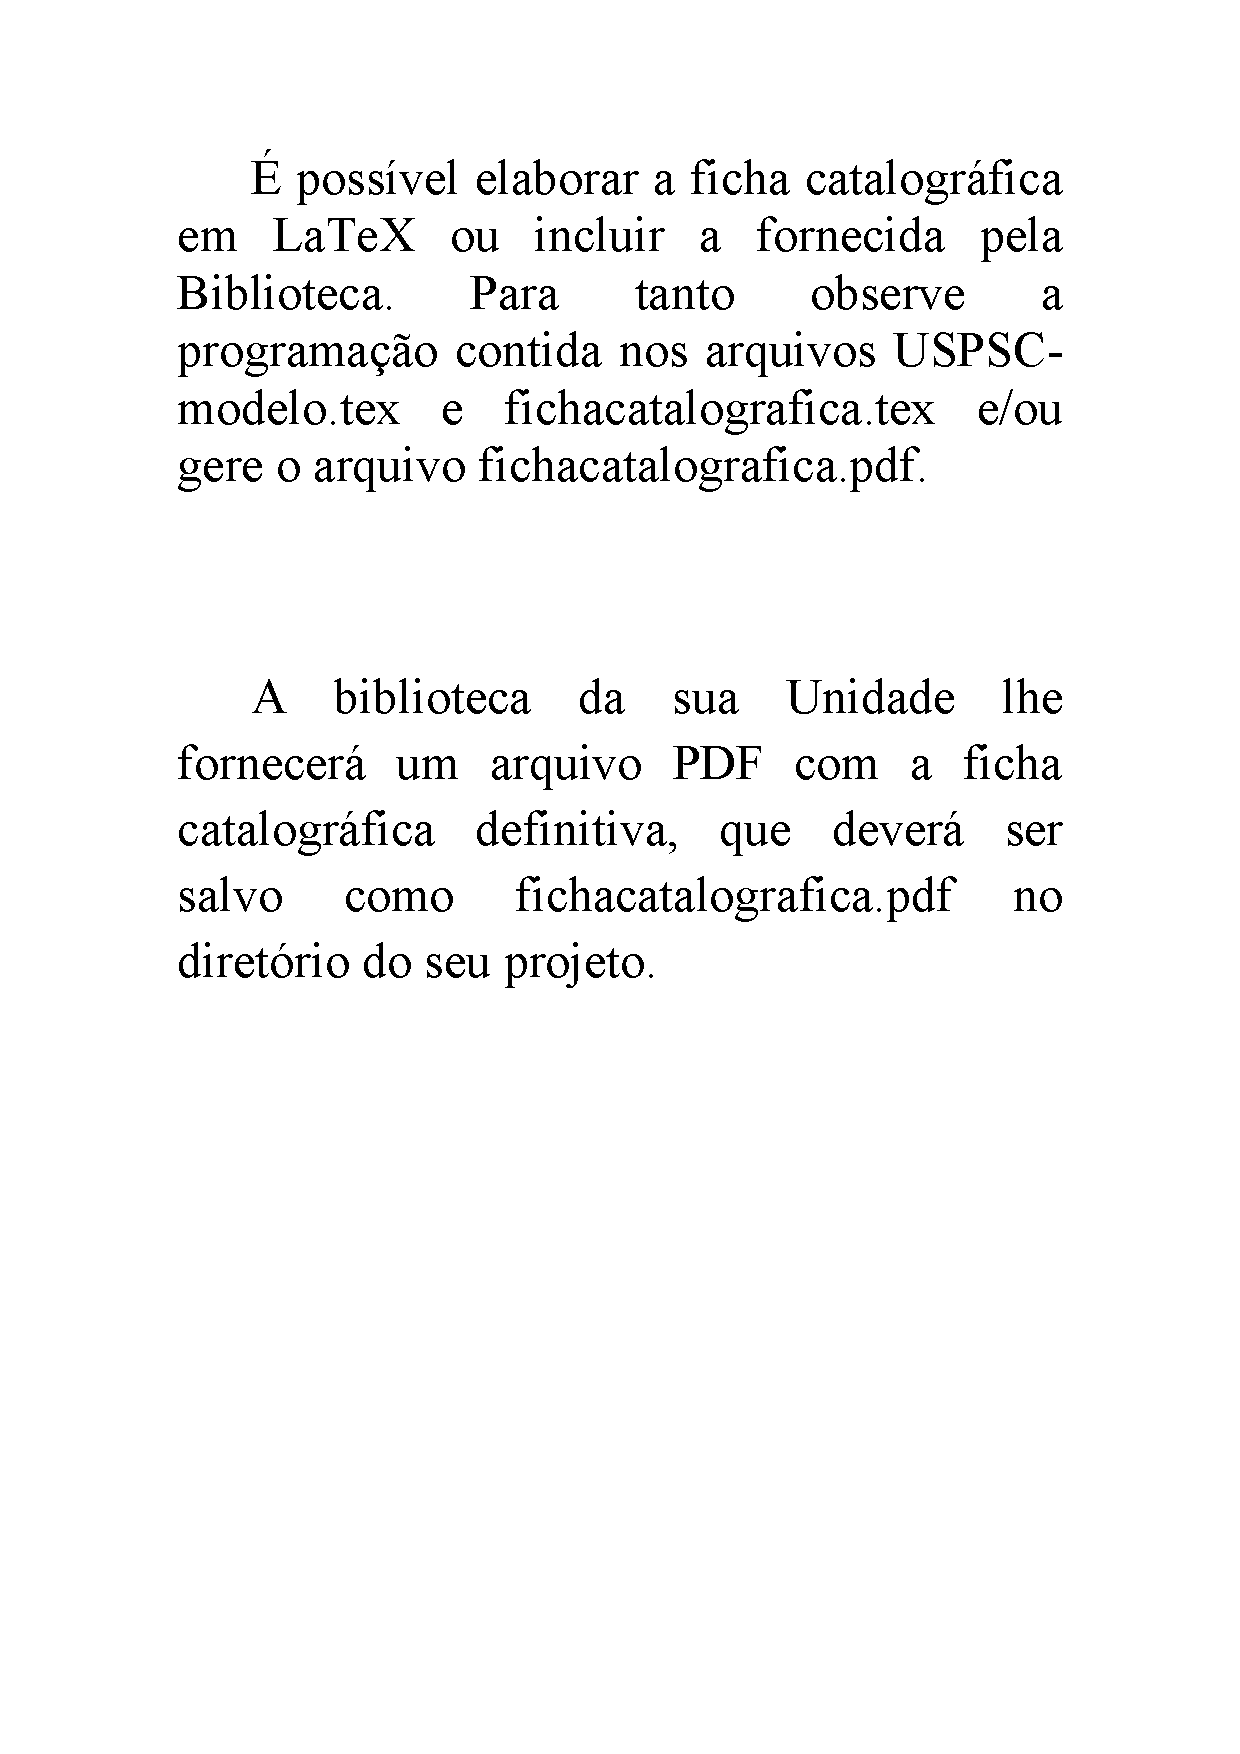
\includepdf{USPSC-TA-PreTextual/USPSC-fichacatalografica.pdf}

% Se voc\^e optar por elaborar a ficha catalogr\'afica, dever\'a 
% incluir uma % antes da linha % antes
% do comando %% USPSC-fichacatalografica.tex
% ---
% Inserir a ficha bibliografica
% ---
% Isto \'e um exemplo de Ficha Catalogr\'afica, ou ``Dados internacionais de
% cataloga\c{c}\~ao-na-publica\c{c}\~ao''. Voc\^e pode utilizar este modelo como refer\^encia. 
% Por\'em, provavelmente a biblioteca da sua universidade lhe fornecer\'a um PDF
% com a ficha catalogr\'afica definitiva ap\'os a defesa do trabalho. Quando estiver
% com o documento, salve-o como PDF no diret\'orio do seu projeto e substitua todo
% o conte\'udo de implementa\c{c}\~ao deste arquivo pelo comando abaixo:
%
\begin{fichacatalografica}
	\hspace{-1.4cm}
	\imprimirnotaautorizacao \\ \\
	%\sffamily
	\vspace*{\fill}					% Posi\c{c}\~ao vertical
\begin{center}					% Minipage Centralizado
  \imprimirnotabib \\
  \begin{table}[htb]
	\scriptsize
	\centering	
	\begin{tabular}{|p{0.9cm} p{8.7cm}|}
		\hline
	      & \\
		  &	  \imprimirautorficha     \\
		
		 \imprimircutter & 
							\hspace{0.4cm}\imprimirtitulo~  / ~\imprimirautor~ ;  ~\imprimirorientadorcorpoficha. -- 	\imprimirlocal, \imprimirdata.   \\
		
		  &  % Para incluir nota referente \`a vers\~ao corrigida no corpo da ficha,
			  % incluir % no in\'{\i}cio da linha acima e tirar a % do in\'{\i}cio da linha abaixo
			  %	\hspace{0.4cm} \imprimirtitulo~  / ~\imprimirautor~ ; ~\imprimirorientadorcorpoficha~- ~\imprimirnotafolharosto. -- \imprimirlocal, \imprimirdata.  \\
		
			\hspace{0.4cm}\pageref{LastPage} p. : il. (algumas color.) ; 30 cm.\\ 
		  & \\
		  & 
		    \hspace{0.4cm}\imprimirnotaficha ~--~ 
						  \imprimirunidademin, 
						  \imprimiruniversidademin, 
		                  \imprimirdata. \\ 
		  & \\                 
		   % Para incluir nota referente \`a vers\~ao corrigida em notas,
		    % incluir uma % no in\'{\i}cio da linha acima e	
		    % tirar a % do in\'{\i}cio da linha abaixo
		    % & \hspace{0.4cm}\imprimirnotafolharosto \\ 
		  & \\ 
		  & \hspace{0.4cm}1. LaTeX. 2. abnTeX. 3. Classe USPSC. 4. Editora\c{c}\~ao de texto. 5. Normaliza\c{c}\~ao da documenta\c{c}\~ao. 6. Tese. 7. Disserta\c{c}\~ao. 8. Documentos (elabora\c{c}\~ao). 9. Documentos eletr\^onicos. I. \imprimirorientadorficha. 
		   II. T\'{\i}tulo. \\
	
		     %Se houver co-orientador, inclua % antes da linha (antes de II. T\'{\i}tulo.) 
		     %          e tire a % antes do comando abaixo 
		     %III. T\'{\i}tulo. \\   
		  \hline
	\end{tabular}
  \end{table}
\end{center}
\end{fichacatalografica}
% ---

 
% e retirar o % do comando abaixo
%%% USPSC-fichacatalografica.tex
% ---
% Inserir a ficha bibliografica
% ---
% Isto \'e um exemplo de Ficha Catalogr\'afica, ou ``Dados internacionais de
% cataloga\c{c}\~ao-na-publica\c{c}\~ao''. Voc\^e pode utilizar este modelo como refer\^encia. 
% Por\'em, provavelmente a biblioteca da sua universidade lhe fornecer\'a um PDF
% com a ficha catalogr\'afica definitiva ap\'os a defesa do trabalho. Quando estiver
% com o documento, salve-o como PDF no diret\'orio do seu projeto e substitua todo
% o conte\'udo de implementa\c{c}\~ao deste arquivo pelo comando abaixo:
%
\begin{fichacatalografica}
	\hspace{-1.4cm}
	\imprimirnotaautorizacao \\ \\
	%\sffamily
	\vspace*{\fill}					% Posi\c{c}\~ao vertical
\begin{center}					% Minipage Centralizado
  \imprimirnotabib \\
  \begin{table}[htb]
	\scriptsize
	\centering	
	\begin{tabular}{|p{0.9cm} p{8.7cm}|}
		\hline
	      & \\
		  &	  \imprimirautorficha     \\
		
		 \imprimircutter & 
							\hspace{0.4cm}\imprimirtitulo~  / ~\imprimirautor~ ;  ~\imprimirorientadorcorpoficha. -- 	\imprimirlocal, \imprimirdata.   \\
		
		  &  % Para incluir nota referente \`a vers\~ao corrigida no corpo da ficha,
			  % incluir % no in\'{\i}cio da linha acima e tirar a % do in\'{\i}cio da linha abaixo
			  %	\hspace{0.4cm} \imprimirtitulo~  / ~\imprimirautor~ ; ~\imprimirorientadorcorpoficha~- ~\imprimirnotafolharosto. -- \imprimirlocal, \imprimirdata.  \\
		
			\hspace{0.4cm}\pageref{LastPage} p. : il. (algumas color.) ; 30 cm.\\ 
		  & \\
		  & 
		    \hspace{0.4cm}\imprimirnotaficha ~--~ 
						  \imprimirunidademin, 
						  \imprimiruniversidademin, 
		                  \imprimirdata. \\ 
		  & \\                 
		   % Para incluir nota referente \`a vers\~ao corrigida em notas,
		    % incluir uma % no in\'{\i}cio da linha acima e	
		    % tirar a % do in\'{\i}cio da linha abaixo
		    % & \hspace{0.4cm}\imprimirnotafolharosto \\ 
		  & \\ 
		  & \hspace{0.4cm}1. LaTeX. 2. abnTeX. 3. Classe USPSC. 4. Editora\c{c}\~ao de texto. 5. Normaliza\c{c}\~ao da documenta\c{c}\~ao. 6. Tese. 7. Disserta\c{c}\~ao. 8. Documentos (elabora\c{c}\~ao). 9. Documentos eletr\^onicos. I. \imprimirorientadorficha. 
		   II. T\'{\i}tulo. \\
	
		     %Se houver co-orientador, inclua % antes da linha (antes de II. T\'{\i}tulo.) 
		     %          e tire a % antes do comando abaixo 
		     %III. T\'{\i}tulo. \\   
		  \hline
	\end{tabular}
  \end{table}
\end{center}
\end{fichacatalografica}
% ---


% As informa\c{c}\~oes que comp\~oem a ficha catalogr\'afica est\~ao 
% definidas no arquivo USPSC-pre-textual-UUUU.tex
% ---

% ---
% Folha de rosto adicional
% Para imprimir a folha de rosto adicional, exigida por algumas Unidades, a exemplo do ICMC,
% retire a % antes do comando abaixo

\imprimirfolhaderostoadic*

% ---
% ---
% Inserir errata
% ---


% ---

% ---
% Inserir folha de aprova\c{c}\~ao
% ---

% A Folha de aprova\c{c}\~ao \'e um elemento obrigat\'orio da NBR 4724/2011 (se\c{c}\~ao 4.2.1.3). 
% Ap\'os a defesa/aprova\c{c}\~ao do trabalho, gere o arquivo folhadeaprovacao.pdf da p\'agina assinada pela banca 
% e iclua o arquivo utilizando o comando abaixo:
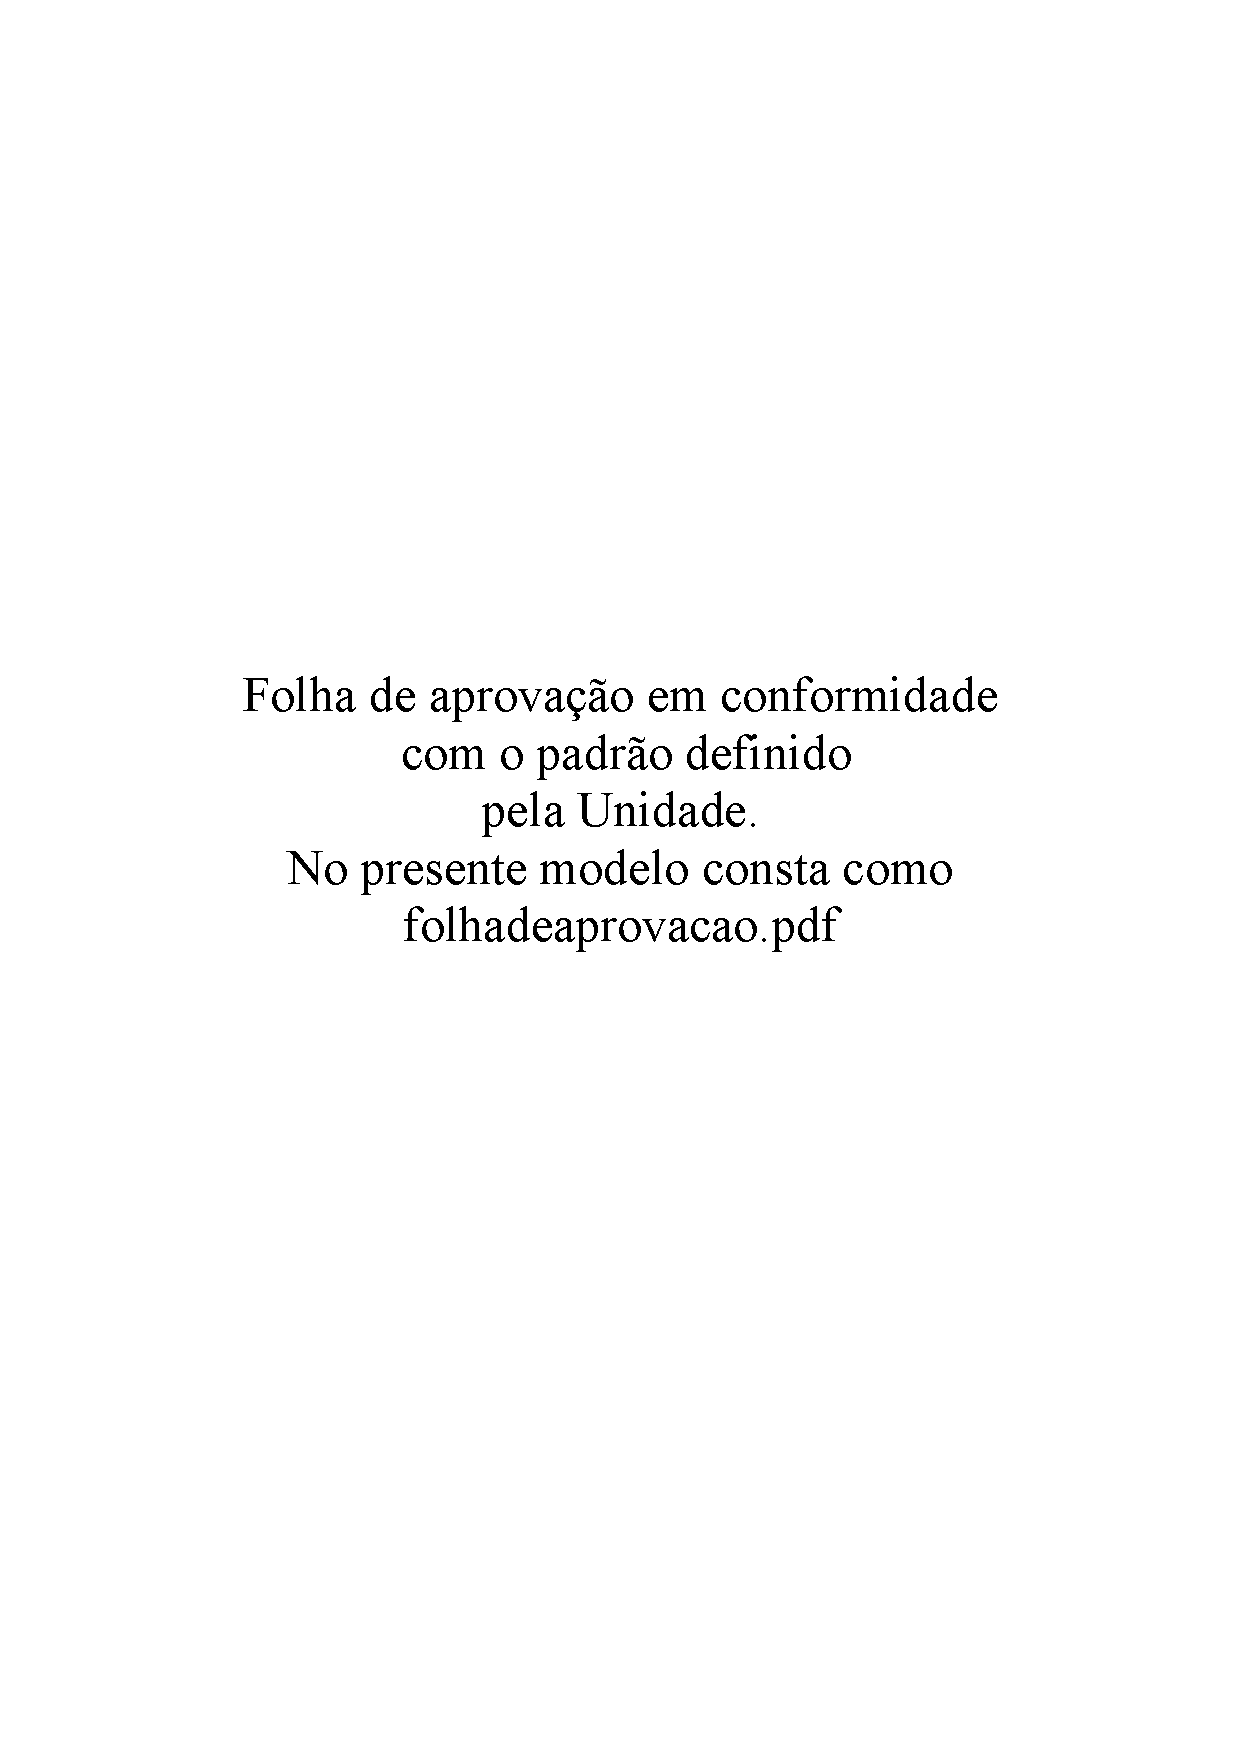
\includepdf{USPSC-TA-PreTextual/USPSC-folhadeaprovacao.pdf}
% Alternativa para a Folha de Aprova\c{c}\~ao:
% Se for a sua op\c{c}\~ao elaborar uma folha de aprova\c{c}\~ao, insira uma % antes do comando acima que inclui o arquivo folhadeaprovacao.pdf,
% tire o % do comando abaixo e altere o arquivo folhadeaprovacao.tex conforme suas necessidades
%\include{folhadeaprovacao}

\includepdf{USPSC-TA-PreTextual/USPSC-PaginaEmBranco.pdf}

% ---
% Dedicat\'oria
% ---
%% USPSC-Dedicatoria.tex
\begin{dedicatoria}
   \vspace*{\fill}
   \centering
   \noindent\textit{@[dedicatoria]@} \vspace*{\fill}
\end{dedicatoria}
% ---
% ---

% ---
% Agradecimentos
% ---
%% USPSC-Agradecimentos.tex
\begin{agradecimentos}
Quero expressar minha gratid\~ao \`as crian\c{c}as e aos jovens; que passaram pelo WASH; que est\~ao conosco e que ser\~ao o futuro do Programa.
Em especial, agrade\c{c}o a uma “crian\c{c}a sempre viva”, ativa, presente, curiosa e que outrora usou o LOGO, gostou de fazer seu jogo e trouxe essa experi\^encia para o seu mundo adulto de cientista, professor, pesquisador, gestor, amigo e companheiro de luta, h\'a mais de uma d\'ecada. Refiro-me ao Dr. Victor Pellegrini Mammana, que ao vivenciar esse prazeroso experimento, quis legar a outras crian\c{c}as o \^extase das descobertas e comprovou que \'e poss\'{\i}vel somar esfor\c{c}os da sociedade civil, das unidades de pesquisa e de educa\c{c}\~ao para contribuir com os processos de aprendizagens em ci\^encia e tecnologia.
Sou, tamb\'em, grata ao meu orientador, Prof. Dr Paulo S\'ergio de Camargo Filho pela companhia e orienta\c{c}\~ao, ao Grupo de Pesquisa STEM Education; e \`a banca de avalia\c{c}\~ao, Prof. Dra. Luciane Capelo e Profº. Dr Eduardo Damasceno.
N\~ao posso deixar de mencionar a generosidade e disposi\c{c}\~ao dos professores Drs. Ala\'{\i}de Pellegrini Mammana e Carlos Mammana, que me forneceram preciosas informa\c{c}\~oes para o trabalho.
Agrade\c{c}o, carinhosamente, \`a Professora Dra. Afira Viana Ripper, por sua contribui\c{c}\~ao para a educa\c{c}\~ao cientifica no ensino fundamental; e por participar do v\'{\i}deo, que resgata essa trajet\'oria e foi parte integrante da minha pesquisa.
Algumas pessoas, tamb\'em, precisam ser destacadas, pois foram imprescind\'{\i}veis para o Programa WASH, desde as suas origens, e marcaram essa hist\'oria (precisei colocar em ordem alfab\'etica): Adriane Pinheiro da Silva, Adriana Tito, Aldo Rabelo, Alex \^Angelo, Alexandre C\^andido Paulo, Alisson Alexandre de Ara\'ujo, Aloizio Mercadante, Am\'elia Naomi, Ant\^onio Carlos dos Santos (o Tot\'o), Ant\^onio Pestana, Alexandre Motta, Ana Paula Rodrigues, Andrea Saraiva, Andrea Dias Victor, Andrea Napolitano, Angel Luis, Antonio Bezerra de Albuquerque, Benedita Aparecida Rodrigues de Freitas, Carlinhos Almeida, C\'assia Oliveira, Cec\'{\i}lia Baranauskas, Celio Turino, Mirza Maria Pellicciotta, Celso Pansera, Celso Pan, Chico Sim\~oes, C\'{\i}ntia Cinquini, Claudio Romanelli, Cleide Santos, Mariana Moura, Clotilde Diogo, Ana Carolina de Deus Soares, Daniel Sp\'ozito, Everbal de Castro, Denise  Vieira Pereira, Dilma Rousseff,  Fabiana Kitagawa, F\'abio Couto, Delma  Medeiros, Fernanda Gon\c{c}alves, Gisele Fink, N\'adia Abiel, Gl\'aucia Veloso, Guida Calixto,  Ingridy Janaina Alves, Haissa Gabriela Silva, Irma Passoni, Isabela Maria Vieira Pereira Rodrigues, Jacqueline Baumgratrz, Jaciara Rodrigues dos Santos, Jandira Maria Rodrigues de Freitas, Jos\'e Leonardo de Oliveira, Juliana Moralles Louvison, Juliana Rabelo, Kevin Martins, Layla Xavier, Leila Bomfim, Let\'{\i}cia Mizael, Lucas Gabriel Batista da Silva, Lucas Titon, Luciano Rudinik, Fernando Accorsi, Magna Gon\c{c}alves, Malu Alencar, Marcela Moreira, Marcelo Aguirre, Maria Fernandes, Michel Morandi Alencar, Nelcina Tropardi. Pedro Tourinho, Paula Ropelo, Paulo B\'ufalo, Priya Patel, Rafael de Deus Soares, Rafael Gomes da Cruz, Rafael Proc\'opio, Renan Inqu\'erito, Renata Xavier, Roberta Santana,  Sandra Lanza, Saulo Monteiro, Sebastian Marques, Tayssa Santana,  S\'ergio Benassi, S\'{\i}lvio Ant\^onio Damasceno, S\'{\i}lvio Aparecido Spinella, TC ( Antonio Carlos), Thatiane Verni Lopes de Ara\'ujo, Toni Klaus, Valdirene Maria dos Santos, Vitor de Oliveira Pochmann, Wagner Rodrigo Silva, Wil Namen, dentre tantos outros.
A todas as gera\c{c}\~oes do WASH: as que passaram, as que compartilham conosco, nesse ano de 2023, os 10 anos do Programa: s\~ao colegas, bolsistas, educandos, educadores, cientistas, coordenadores, orientadores, Conselhos de classes, Sindicatos, gestores, pesquisadores, vereadores, comunidades, os entes federados, que acreditam na ci\^encia e no papel transformador da educa\c{c}\~ao.
Meus agradecimentos, tamb\'em. \`as institui\c{c}\~oes parceiras: Conselho Nacional de Desenvolvimento Cient\'{\i}fico e Tecnol\'ogico - CNPq , Funda\c{c}\~ao Arauc\'aria, WASH Paran\'a, Cia Bola de Meia, Legislativo Federal, por meio dos deputados: Ivan Valente, Alex e Luiza Canziani, Alexandre Padilha, Vicentinho, Carlos Zaratini, Orlando Silva e Alexandre Cury, que foram sens\'{\i}veis e valorizaram a educa\c{c}\~ao cientifica, atrav\'es do Programa WASH. Aos legislativos de Prado Ferreira e Dr. Camargo por fazerem o WASH leis municipais. N\~ao posso deixar de reconhecer a contribui\c{c}\~ao da AkiPosso , com o apoio dos colegas Kevin Martins, Adriana Tito, Priya Patel, Caroline Gardemann, Nelcina Tropardi e Daniela Napolitano. Por fim, agrade\c{c}o a minha fam\'{\i}lia, a minha filha, Agatha Abayomi Silva Sene, aos meus pais, Maria Imaculada de Oliveira e Silva e Joaquim Roberto da Silva, ao meu irm\~ao Eduardo Roberto da Silva in memoriam - presente! e ao Alessandro, que contribu\'{\i}ram para que as condi\c{c}\~oes necess\'arias para o desenvolvimento dessa pesquisa fossem as mais leves para a execu\c{c}\~ao do meu estudo.
Termino enfatizando os papeis especiais do Vereador Paulo Bufalo, que est\'a nesta caminhada conosco desde os prim\'ordios do programa, e da Dra. Andrea Dias Victor, servidora do CNPq que permanece aceitando, com compromisso p\'ublico, excel\^encia administrativa e acad\^emica, a carga de gest\~ao do programa WASH, representada por centenas de bolsistas semestrais.
% @[pontoinsercaoparagrafoagradecimento]@

\end{agradecimentos}
% ---
% ---

% ---
% Ep\'{\i}grafe
% ---
%% USPSC-Epigrafe.tex
\begin{epigrafe}
    \vspace*{\fill}
	\begin{flushright}\textit{. Brasil Meu Brasil ande pra frente. Venha com a gente pra Avenida desfilar . \'E chegada a hora da verdade. N\~ao \'e preciso mais voc\^e se disfar\c{c}ar. Levante os panos, mostra tua cara. E assuma essa cara que voc\^e tem. Brasil Terra dos Ianom\^amis. Essas matas s\~ao de Oxossi. Deixa na terra as riquezas de Oxum. Devolva pro povo o que \'e do povo. Bote os malditos pra fora. E vamos refazer essa na\c{c}\~ao. Pois,o pa\'{i}s que  \'e o olho d’\'agua do mundo n\~ao pode ver sofrer. N\~ao pode ver chorar um povo que trabalha, canta e \'e feliz. Chega de tanta injusti\c{c}a, chega de corrup\c{c}\~ao. Vamos arrumar a casa, vamos dividir o nosso ch\~ao. E chega de sofrer e chega de chorar. Oh p\'atria amada idolatrada. Salve-se Brasil! Antonio Carlos (TC) Santos Silva Alu\'{i}zio Jeremias (Samba Enredo, 1988)}
	\end{flushright}
\end{epigrafe}
% ---
% ---

% A T E N \c{C} \~A O
% Se o idioma do texto for em ingl\^es, o abstract deve preceder o resumo
% resumo em portugu\^es
%
% Resumo
% ---
%% USPSC-Resumo.tex
\setlength{\absparsep}{18pt} % ajusta o espa\c{c}amento dos par\'agrafos do resumo
\begin{resumo}
\begin{flushleft} 
\setlength{\absparsep}{0pt} % ajusta o espa\c{c}amento da refer\^encia
\SingleSpacing 
\imprimirautorabr~~\textbf{\imprimirtituloresumo}.\imprimirdata. \pageref{LastPage}p. 
%Substitua p. por f. quando utilizar oneside em \documentclass
%\pageref{LastPage}f.
\imprimirtipotrabalho~-~\imprimirinstituicao, \imprimirlocal, \imprimirdata. 
 \end{flushleft}
\OnehalfSpacing 
O  Programa Workshop de Aficcionados em Software e Hardware (WASH), de educa\c{c}\~ao em Ci\^encia, Tecnologia, Engenharia, Artes e Matem\'atica (STEAM) \'e executado desde 2013 em dezenas de munic\'{\i}pios brasileiros e com milhares de crian\c{c}as atendidas. Ap\'os anos de pr\'atica, as caracter\'{\i}sticas principais foram agrupadas no Documento de Refer\^encia publicado em 2018, anexado \`a Portaria CTI 178/2018. Esta pesquisa \'e dividida em 2 eixos: m\'etodo historiogr\'afico (eixo 1) e o emprego de consultas estruturadas a uma base de dados especialmente desenvolvida para produzir os indicadores (eixo 2). O trabalho buscou comparar, a partir das defini\c{c}\~oes do Documento de Refer\^encia, \textquotedbl\{\}o que o WASH gostaria de ter sido\textquotedbl\{\} com \textquotedbl\{\}o que o WASH conseguiu ser\textquotedbl\{\}, informa\c{c}\~ao decorrente dos Resultados e An\'alise desta disserta\c{c}\~ao. Para objetivar essa compara\c{c}\~ao, foram formuladas seis hip\'oteses, a partir do Documento de Refer\^encia, que ao final do trabalho foram submetidas a uma valida\c{c}\~ao.  A an\'alise dos sucessos e insucessos dessa valida\c{c}\~ao permitiu produzir uma revis\~ao do Documento de Refer\^encia, a qual \'e o principal produto educacional desta disserta\c{c}\~ao, quesito obrigat\'orio para a obten\c{c}\~ao do t\'{\i}tulo em Mestrado. Agrega-se a esse produto educacional a entrevista com a Profa. Afira Ripper, um dos elementos usados para a an\'alise no eixo 1 e, tamb\'em, um testemunho bastante raro sobre a vinda de Seymour Papert ao Brasil no final do s\'eculo passado.
% @[pontoinsercaoparagraforesumo]@
 

 \textbf{Palavras-chave}: Papert, STEAM, STEM, WASH
\end{resumo}
% ---

% Abstract
% ---
%% USPSC-Abstract.tex
%\autor{Silva, M. J.}
\begin{resumo}[Abstract]
 \begin{otherlanguage*}{english}
	\begin{flushleft} 
		\setlength{\absparsep}{0pt} % ajusta o espaçamento dos par\'agrafos do resumo		
 		\SingleSpacing  		\imprimirautorabr~~\textbf{\imprimirtitleabstract}.	\imprimirdata.  \pageref{LastPage}p. 
		%Substitua p. por f. quando utilizar oneside em \documentclass
		%\pageref{LastPage}f.
		\imprimirtipotrabalhoabs~-~\imprimirinstituicao, \imprimirlocal, 	\imprimirdata. 
 	\end{flushleft}
	\OnehalfSpacing 
   This is the english abstract.

   \vspace{\onelineskip}
 
   \noindent 
   \textbf{Keywords}: LaTeX. USPSC class. Thesis. Dissertation. Conclusion course paper. 
 \end{otherlanguage*}
\end{resumo}

% ---

% ---
% inserir lista de figurass
% ---
\pdfbookmark[0]{\listfigurename}{lof}
\listoffigures*
\cleardoublepage
% ---

% ---
% inserir lista de tabelas
% ---
\pdfbookmark[0]{\listtablename}{lot}
\listoftables*
\cleardoublepage
% ---

% ---
% inserir lista de quadros
% ---
\pdfbookmark[0]{\listofquadroname}{loq}
\listofquadro*
\cleardoublepage
% ---

% ---
% inserir lista de abreviaturas e siglas
% ---
% USPSC-AbreviaturasSiglas.tex
\begin{siglas}
    \item[ABNT] Associação Brasileira de Normas Técnicas
    \item[abnTeX] ABsurdas Normas para TeX
	\item[IBGE] Instituto Brasileiro de Geografia e Estatística
	\item[LaTeX] Lamport TeX
	\item[USP] Universidade de São Paulo
	\item[USPSC] Campus USP de São Carlos
\end{siglas}

% ---

% ---
% inserir lista de s\'{\i}mbolos
% ---
% USPSC-Simbolos.tex
\begin{simbolos}
  \item[$ \Gamma $] Letra grega Gama
  \item[$ \Lambda $] Lambda
  \item[$ \zeta $] Letra grega minúscula zeta
  \item[$ \in $] Pertence
\end{simbolos}
% ---
% ---
% inserir o sumario
% ---
\pdfbookmark[0]{\contentsname}{toc}
\tableofcontents*
\cleardoublepage
% ---
% ----------------------------------------------------------
% ELEMENTOS TEXTUAIS
% ----------------------------------------------------------
\textual
% Os cap\'{\i}tulos s\~ao inseridos como arquivos externos 

% Cap\'{\i}tulo 1 - Introdu\c{c}\~ao
% ---
\chapter[INTRODU\c{C}\~AO]{INTRODU\c{C}\~AO}\label{INTRODU\c{C}\~AO}
Aos olhos de jovens observadores contempor\^aneos, parece natural a relativa desenvoltura com que as pessoas utilizam  as tecnologias da informa\c{c}\~ao e comunica\c{c}\~ao em computadores e celulares nos dias de hoje. J\'a est\~ao bastante difundidos os servi\c{c}os de governo eletr\^onico, os sites de com\'ercio, os  aplicativos de entrega, as plataformas de ensino, de reuni\~oes, a busca por oportunidades profissionais, urna eletr\^onica, os servi\c{c}os financeiros e de caixa eletr\^onico, por exemplo.










Desta forma, \'e poss\'{\i}vel afirmar que as pessoas t\^em usado com frequ\^encia e com relativa facilidade as ferramentas digitais instaladas em computadores e em celulares, sejam aplicativos de mensagens, buscadores (browsers), correio eletr\^onico, redes sociais, entre outras. Este uso d\'a-se em v\'arios contextos: profissional, educacional, de sa\'ude,  de entretenimento e de intera\c{c}\~ao social.










As novas gera\c{c}\~oes precisam, no entanto, saber que n\~ao foi sempre assim. Muito embora a percep\c{c}\~ao corrente de que o uso de computadores e celulares \'e indispens\'avel para o conv\'{\i}vio na sociedade, a rigor seu uso \'e relativamente recente.










\'E poss\'{\i}vel identificar a evolu\c{c}\~ao das telecomunica\c{c}\~oes a partir do s\'eculo passado como origem das transforma\c{c}\~oes tecnol\'ogicas que disponibilizaram tecnologias digitais em larga escala. Esta evolu\c{c}\~ao foi identificada, por exemplo, por PIERRE LEVY, no texto \textquotedbl Cibercultura\textquotedbl  (LEVY, 2000):











\noindent\begin{center}\mbox{\centering\fbox{\centering\par\parbox{0.7\linewidth}{\small\textit{\textquotedbl Durante uma entrevista nos anos 50, Albert Einstein (1879-1955) declarou que tr\^es grandes bombas haviam  explodido durante o s\'eculo XX: a bomba demogr\'afica, a bomba at\^omica e a bomba das telecomunica\c{c}\~oes. Aquilo que Einstein chamou de bomba das telecomunica\c{c}\~oes foi chamado, por meu amigo Roy Ascott (um dos pioneiros e principais te\'oricos da arte em rede), de segundo dil\'uvio, o das informa\c{c}\~oes. As telecomunica\c{c}\~oes geram esse novo dil\'uvio por conta da natureza exponencial, explosiva e ca\'otica de seu crescimento. A quantidade bruta de dados dispon\'{\i}veis se multiplica e se acelera. A densidade dos links entre as informa\c{c}\~oes aumenta vertiginosamente nos bancos de dados, nos hipertextos  e nas redes.\textquotedbl }\normalsize}}}\end{center}


Ainda, segundo Pierre Levy,











\noindent\begin{center}\mbox{\centering\fbox{\centering\par\parbox{0.7\linewidth}{\small\textit{\textquotedbl O segundo dil\'uvio n\~ao ter\'a fim. N\~ao h\'a nenhum fundo s\'olido sob o oceano de informa\c{c}\~oes. Devemos aceit\'a-lo como nossa nova condi\c{c}\~ao. Temos que ensinar nossos filhos a nadar, a flutuar, talvez a navegar.\textquotedbl }\normalsize}}}\end{center}


Para a sociedade chegar nesse ponto, seus governos e iniciativa privada tiveram que, continuamente, investir no desenvolvimento de inova\c{c}\~oes cient\'{\i}ficas e tecnol\'ogicas,  provendo, com base nessas inova\c{c}\~oes, a infraestrutura de comunica\c{c}\~oes e de redes digitais, bem como os meios de acesso a essas redes.










Em outra ponta, tiveram que formular pol\'{\i}ticas p\'ublicas para preparar os cidad\~aos e cidad\~as para que pudessem se apropriar dessas tecnologias.










Inicialmente, a partir da segunda metade do s\'eculo XX, as redes digitais estavam fortemente vinculadas \`a academia, \`as institui\c{c}\~oes de pesquisa e \`a \'area de defesa  (ARPANET, 2022), principalmente num contexto de coordena\c{c}\~ao estatal.










Posteriormente, a partir do in\'{\i}cio da \'ultima d\'ecada do s\'eculo XX, essas inova\c{c}\~oes  foram avan\c{c}ando em dire\c{c}\~ao ao suprimento das necessidades de relacionamento do cidad\~ao com o governo. Mas, a partir da segunda metade dessa mesma d\'ecada, os servi\c{c}os baseados nestas inova\c{c}\~oes foram mais longe, e alcan\c{c}aram  as demais facetas dos indiv\'{\i}duos, inclusive na sua rela\c{c}\~ao com os prestadores de servi\c{c}os privados.










Essa expans\~ao deu-se como resultado de v\'arias a\c{c}\~oes, mas sua universaliza\c{c}\~ao foi resultado principalmente do surgimento de novas formas de relacionamento social viabilizadas pelas redes digitais, que tornaram mais acess\'{\i}veis novas ferramentas de apoio ao ensino em sala de aula, ao ensino \`a dist\^ancia, ao com\'ercio eletr\^onico, \`a elei\c{c}\~ao eletr\^onica, aos \textquotedbl market-places\textquotedbl , aos aplicativos de transporte e entrega, ao agendamento de eventos, reuni\~oes e consultas m\'edicas, dentre tantos outros exemplos.










Tais transforma\c{c}\~oes tiveram impactos econ\^omicos e sociais profundos, inclusive nas rela\c{c}\~oes de trabalho, tanto na cria\c{c}\~ao e extin\c{c}\~ao de postos de trabalho, como em suas formas de contrata\c{c}\~ao, jornada, remunera\c{c}\~ao, inclusive com a precariza\c{c}\~ao dos direitos trabalhistas. Elas est\~ao muito bem descritas  no relat\'orio da Unesco  de 2004 \textquotedbl Social Transformation in an Information Society: Rethinking Access to You and the World\textquotedbl  (DUTTON, 2004).










A amplitude destas transforma\c{c}\~oes foi sintetizada no conceito de \textquotedbl Sociedade da Informa\c{c}\~ao\textquotedbl , \`as vezes referido como \textquotedbl Era Digital\textquotedbl  ou \textquotedbl Era da Informa\c{c}\~ao\textquotedbl .










O efeito dessas transforma\c{c}\~oes no emprego vem exigindo dos governos, das empresas e dos cidad\~aos uma constante e r\'apida readapta\c{c}\~ao  das rela\c{c}\~oes de trabalho e da produ\c{c}\~ao de novos saberes e compet\^encias. Consequentemente, tamb\'em o sistema educacional vem sendo desafiado a se adaptar, uma vez que \'e dele que se espera o preparo dos cidad\~aos para a nova realidade. Aqueles cidad\~aos que n\~ao se prepararem correm o risco constante de ficar sem sustento.










Inicialmente tais transforma\c{c}\~oes eram associadas principalmente \`a substitui\c{c}\~ao do trabalho humano decorrente da automa\c{c}\~ao industrial. Mas a radicaliza\c{c}\~ao no uso de solu\c{c}\~oes digitais, inclusive de intelig\^encia artificial, associadas ao aumento da conectividade, v\^em substituindo capacidades \textquotedbl cognitivas que antes eram exclusivas de humanos\textquotedbl [4 XXX]. Uma das consequ\^encias mais radicais \'e o surgimento de novos meios de explora\c{c}\~ao humana, representados pela \textquotedbl Gigs Economy\textquotedbl   (Manyika, 2016), ou \textquotedbl Economia do Bico\textquotedbl , que precariza as rela\c{c}\~oes trabalhistas por meio de plataformas que as impessoaliza a ponto de camuflar a explora\c{c}\~ao. O termo \textquotedbl bico\textquotedbl  aqui est\'a sendo usado como tradu\c{c}\~ao livre de \textquotedbl gigs\textquotedbl , que nos Estados Unidos \'e uma g\'{\i}ria usada para trabalho tempor\'ario. A uberiza\c{c}\~ao \'e um exemplo de rela\c{c}\~ao de trabalho no contexto da Gigs Economy.










V\'arios pa\'{\i}ses t\^em buscado uma melhor prepara\c{c}\~ao para enfrentar essas transforma\c{c}\~oes, dotando o cidad\~ao de meios cognitivos, de conhecimento e cultura para se readaptar. Para isso, t\^em procurado remodelar seus sistemas educacionais, uma vez que “ficar para tr\'as em educa\c{c}\~ao”, em rela\c{c}\~ao aos demais pa\'{\i}ses, pode afetar a prosperidade (CONGRESS, 1998)  de suas popula\c{c}\~oes, sua autonomia e liberdade.










Mais do que simplesmente \textquotedbl treinar\textquotedbl  os cidad\~aos quanto ao uso  de servi\c{c}os digitais, a educa\c{c}\~ao tem um papel fundamental de prepar\'a-los para sua inser\c{c}\~ao aut\^onoma e digna na sociedade transformada pelas tecnologias de informa\c{c}\~ao e comunica\c{c}\~ao. Portanto, o desafio do Estado n\~ao se limita a estabelecer pol\'{\i}ticas p\'ublicas de provimento de infraestrutura para que o cidad\~ao possa ter acesso e se beneficiar dos recursos digitais e de comunica\c{c}\~ao, mas, principalmente, preparar estes cidad\~aos para que contribuam com a  constru\c{c}\~ao desses recursos, beneficiando-se da autonomia e prosperidade que  essa constru\c{c}\~ao gera.










O cidad\~ao tamb\'em precisa ser capaz de entender \textquotedbl o que est\'a por tr\'as\textquotedbl  desses sistemas digitais, para que possa reagir aos excessos da \textquotedbl algoritmiza\c{c}\~ao\textquotedbl  de suas rela\c{c}\~oes com outros indiv\'{\i}duos.










Assim, antecipando aqui uma das conclus\~oes desta disserta\c{c}\~ao, \'e no contexto do \textquotedbl segundo dil\'uvio\textquotedbl , considerando a bomba das telecomunica\c{c}\~oes e da inform\'atica, que se insere a necessidade de um projeto educacional como o WASH.










A percep\c{c}\~ao da import\^ancia da educa\c{c}\~ao para a prosperidade da sociedade n\~ao \'e uma not\'{\i}cia nova. No caso americano, por exemplo, remonta aos prim\'ordios de sua independ\^encia. Em termos globais \'e poss\'{\i}vel perceber o reconhecimento de sua import\^ancia desde a gr\'ecia e do Egito antigos.










No cap\'{\i}tulo \textquotedbl Fundamenta\c{c}\~ao Te\'orica\textquotedbl  revisaremos as origens do conceito de \textquotedbl Science, Technology, Engineering and Mathematics\textquotedbl  (STEM), mostrando que j\'a em 1790 o presidente George Washington, em seu primeiro discurso do \textquotedbl Estado da Uni\~ao\textquotedbl  enaltecia a ci\^encia e a literatura como  base da \textquotedbl felicidade p\'ublica\textquotedbl  [XXX]. Essa percep\c{c}\~ao de valor da ci\^encia e da cultura perdurou hist\'oria americana, at\'e os dias de hoje. Em muitos momentos foi estimulada, inclusive, como resposta \`as amea\c{c}as externas, como foi o caso da mobiliza\c{c}\~ao americana para fazer frente ao sucesso sovi\'etico no programa espacial, representado pelo pioneirismo do lan\c{c}amento do sat\'elite Sputnik no final da d\'ecada de 50. \'E naquele cen\'ario da Guerra Fria que a pol\'{\i}tica de educa\c{c}\~ao em STEM e alfabetiza\c{c}\~ao cient\'{\i}fica e tecnol\'ogica passou a ser vista mais claramente como um bem comum, mesmo muito antes do uso desse acr\^onimo de forma oficial. (Relat\'orio CRS para o Congresso, www.crs.gov, 2012)










N\~ao obstante esta permanente percep\c{c}\~ao p\'ublica da import\^ancia e do valor da ci\^encia, os Estados Unidos n\~ao conseguiram manter uma forma\c{c}\~ao de qualidade nas \'areas STEM.










Nos anos 90 os EUA identificaram fragilidades na educa\c{c}\~ao de STEM com preju\'{\i}zo ao \textquotedbl poderio b\'elico e tecnol\'ogico nacional\textquotedbl , \`a inser\c{c}\~ao de seus cidad\~aos no novo mundo do trabalho, de forma aut\^onoma, soberana  e pr\'ospera. Essas fragilidades foram evidenciadas pelo recorrente e relativamente baixo desempenho de adolescentes americanos no \textquotedbl Programme for International Student Assessment\textquotedbl  (PISA)  (CATTERALL, 2017). Com isso, o governo americano teve que propor a\c{c}\~oes para atualizar as compet\^encias curriculares, visando manter uma inser\c{c}\~ao hegem\^onica na economia do s\'eculo XXI.










Segundo Relat\'orio do \textquotedbl Congress Research Service\textquotedbl  (CRS - Servi\c{c}o de pesquisa do Congresso Americano), mais de 200 projetos de Lei contendo o termo \textquotedbl educa\c{c}\~ao cient\'{\i}fica\textquotedbl  foram apresentados entre 1987 e 2008. O mesmo relat\'orio aponta que 13 ag\^encias federais estavam envolvidas em programas ou atividades de educa\c{c}\~ao do tipo \textquotedbl STEM\textquotedbl . (Pag.2 do Relat\'orio).










Os atores governamentais e estudiosos daquele per\'{\i}odo identificaram que faltava aos EUA uma pol\'{\i}tica nacional uniforme e inclusiva de ensino de ci\^encias, pois era poss\'{\i}vel categorizar diferentes \^enfases sobre o assunto no vasto sistema educacional americano  (CATTERALL, 2017).










Mas existia tamb\'em o reconhecido pioneirismo da comunidade acad\^emica americana nos m\'etodos voltados para o aprendizado de temas relacionados ao STEM, ainda que n\~ao identificados sob esse acr\^onimo ou mesmo que n\~ao amplamente disseminados em seu sistema educacional, como viriam a reconhecer os relat\'orios do congresso americano  (CONGRESS, 1998).










Seymour Papert, matem\'atico sul-africano radicado nos EUA, do Laborat\'orio de Intelig\^encia Artificial do Massachusetts Institute of Technology (MIT), foi um  cientista e educador que acreditava  no  uso do computador como forma de revolucionar o sistema  educacional  desde os anos 60.










Ele foi um cientista vision\'ario ao pensar a aprendizagem de crian\c{c}as de forma diferente. Em 1968 escreveu o artigo \textquotedbl  Teaching Children Thinking \textquotedbl   em que abordava  o tema sobre crian\c{c}as, educa\c{c}\~ao e computadores. No cap\'{\i}tulo de Fundamenta\c{c}\~ao te\'orica sua contribui\c{c}\~ao ser\'a aprofundada, mas \'e necess\'ario antecipar aqui alguns elementos para que seja poss\'{\i}vel delimitar o escopo da presente pesquisa.










O carat\'er pioneiro do pensamento de Papert ficar\'a mais evidente na fundamenta\c{c}\~ao te\'orica. Entretanto, cabe reconhecer aqui, de forma resumida, que, quando formulou suas ideias, nos anos 70, os computadores  ainda n\~ao eram amplamente acess\'{\i}veis ou dispon\'{\i}veis para uso dom\'estico ou nas escolas.










Naquele tempo n\~ao existia o conceito de \textquotedbl micro-computadores\textquotedbl . Equipamentos com poder de processamento milhares de vezes inferior ao de um notebook de hoje, ocupavam centenas de metros quadrados  (CIPOLI, 2012) . Segundo  SOLOMON et al. (2020) , \textquotedbl em 1966 os computadores eram poucos, grandes e espalhados\textquotedbl , os custos eram muito altos e, portanto, o acesso era muito restrito.










Mas mesmo na forma de mainframes centralizados (computadores de grande porte) com as limita\c{c}\~oes indicadas acima, foi poss\'{\i}vel a Papert realizar incurs\~oes desbravadoras no campo da aprendizagem para crian\c{c}as utilizando computadores, ainda que sem uma ampla dissemina\c{c}\~ao no sistema educacional americano.










Uma gera\c{c}\~ao de educadores foi formada em torno das ideias de Papert, para quem a aprendizagem de linguagem de programa\c{c}\~ao de computadores, j\'a no ensino fundamental, poderia ter um papel importante no aprendizado de muitas outras disciplinas tradicionais, tais como matem\'atica, ci\^encias e linguagem. A proposta de Papert, at\'e por enfatizar o aprendizado de crian\c{c}as, n\~ao tinha qualquer ambi\c{c}\~ao de capacita\c{c}\~ao profissional e, por si s\'o, n\~ao visava diretamente fazer frente aos desafios do \textquotedbl mundo do trabalho\textquotedbl , que foram sendo introduzidos pelas transforma\c{c}\~oes inerentes \`a Sociedade da Informa\c{c}\~ao nas d\'ecadas subsequentes. Para Papert o computador poderia funcionar como o indutor da aprendizagem de muitas disciplinas.










Diferentemente de um simples treinamento para usar computadores, o m\'etodo de Papert representava uma mudan\c{c}a em paradigmas educacionais, focalizando a aprendizagem em detrimento do ensino  (NEGROPONTE, 2004) . A ideia era \textquotedbl aprender o que se precisa\textquotedbl  e n\~ao \textquotedbl aprender o que se deve\textquotedbl .










O car\'ater estritamente educacional e a peculiar abordagem das propostas de Papert s\~ao apontados em \textquotedbl Brazil Plan\textquotedbl   (NEGROPONTE, 2004) , embora muito a posteriori por seus colegas, como uma alternativa para a inser\c{c}\~ao do indiv\'{\i}duo na \textquotedbl era digital\textquotedbl  (digital age).










Assumindo que o conceito de \textquotedbl era digital\textquotedbl  se refere \`as transforma\c{c}\~oes tecnol\'ogicas que viabilizaram a  \textquotedbl Sociedade da Informa\c{c}\~ao\textquotedbl ,  \'e razo\'avel depreender, a partir do que est\'a presente em Brazil Plan  (NEGROPONTE, 2004), que seus sucessores no MIT, de forma independente, entendiam a proposta de Papert como um caminho natural para a melhor inser\c{c}\~ao dos indiv\'{\i}duos na Sociedade da Informa\c{c}\~ao.










O pioneirismo de Papert permite reconhecer nele uma inspira\c{c}\~ao para as demais iniciativas educacionais no estilo STEM que vieram depois. Estas iniciativas propunham uma educa\c{c}\~ao despojada de formalismos, voltada para a resolu\c{c}\~ao de problemas, ao inv\'es da hist\'orica obsess\~ao por conte\'udos. Esse tipo de abordagem inspirou boa parte dos conceitos subjacentes  \textquotedbl maker culture\textquotedbl , entre outros.










As preocupa\c{c}\~oes com o relativo baixo desempenho em STEM, que se aprofundavam nos EUA nos anos 90, alcan\c{c}aram o resto do mundo. Come\c{c}aram a surgir propostas para tentar promover a qualifica\c{c}\~ao da educa\c{c}\~ao em pa\'{\i}ses em desenvolvimento por meio do uso intensivo de computadores, nos moldes do que enxergara Papert em seus trabalhos seminais.










Dentre estas propostas destaca-se o \textquotedbl One Laptop per Child\textquotedbl , projeto elaborado por pesquisadores do MIT  (NEGROPONTE, 2004)  sucessores dos trabalhos seminais de Papert. Uma descri\c{c}\~ao detalhada sobre as caracter\'{\i}sticas e hist\'oria do OLPC pode ser encontrada no cap\'{\i}tulo de Resultados e An\'alises, bem como em outras refer\^encias  (ALVAREZ, 2015).










Neste ponto podemos sintetizar que o OLPC envolvia a distribui\c{c}\~ao massiva de laptops (notebooks) para crian\c{c}as e adolescentes do  ensino fundamental e m\'edio, com vistas a universalizar o acesso \`a internet no \^ambito da escola p\'ublica brasileira.










Esta universaliza\c{c}\~ao visava oportunizar v\'arias pr\'aticas pedag\'ogicas no \^ambito da Escola P\'ublica, dentre elas a programa\c{c}\~ao de computadores, consequ\^encia direta do pensamento de Papert. Para que pudesse ser implementada nos prazos e formato pretendidos pelo MIT, a proposta OLPC comprometeria boa parcela do or\c{c}amento do Minist\'erio da Educa\c{c}\~ao na compra de laptops (notebooks). Foi esse comprometimento, e o risco a ele associado, que estimulou o Governo Brasileiro a buscar formas de avaliar sua efetividade.










O Programa WASH nasceu  (MAMMANA e TOZZI, 2018)  como uma proposta alternativa ao OLPC, com custo inferior, que n\~ao exigia a aquisi\c{c}\~ao de milh\~oes de equipamentos, mas que se inspirava nos mesmos conceitos exitosos de Papert que fundamentaram a proposta do OLPC.










Assim, o Programa WASH buscou centrar-se na cria\c{c}\~ao de espa\c{c}os de intera\c{c}\~ao no contexto de valores do m\'etodo cient\'{\i}fico, buscando estabelecer meios para estimular, inicialmente, as disciplinas de STEM e, posteriormente, incluindo arte na lista, como tantos outros autores fizeram naquele per\'{\i}odo  (CATTERALL, 2017) (MAMMANA e TOZZI, 2018)  (YAKMAN, 2019). Desta forma, um novo acr\^onimo nasceu agregando Science, Technology Engineering, Arts and Mathematics, o STEAM  (YAKMAN, 2019).










A avalia\c{c}\~ao do Projeto OLPC proporcionou uma resignifica\c{c}\~ao para a proposta, permitindo compreender mais profundamente os desafios do uso intensivo de tecnologia da informa\c{c}\~ao no contexto da escola p\'ublica brasileira e, com isso, propor uma alternativa.










O WASH se constitui em atividades em grupo, realizadas no contraturno, desvinculadas do curr\'{\i}culo tradicional da escola formal, cujos valores principais se alicer\c{c}am no m\'etodo cient\'{\i}fico. O WASH n\~ao \'e um curso, mas se constitui em espa\c{c}os de intera\c{c}\~ao humana para experimenta\c{c}\~ao e conviv\^encia entre indiv\'{\i}duos, no contexto do desenvolvimento de projetos de v\'arios n\'{\i}veis de complexidade.










Pela forma como os pilotos do WASH acabaram sendo implementados no contexto do CTI Renato Archer, houve a consolida\c{c}\~ao da vis\~ao de que institui\c{c}\~oes de P










Hoje o Programa WASH tem seu m\'etodo descrito por meio de um documento de refer\^encia, a Portaria CTI 178/2018, que estabelece uma \textquotedbl liturgia\textquotedbl   (MAMMANA et al., 2020) de realiza\c{c}\~ao de oficinas, os papeis de cada participante e a forma de opera\c{c}\~ao. Mas \'e evidente que, por ser longevo, alcan\c{c}ando em 2023 a marca de 10 anos de realiza\c{c}\~ao, o WASH passou por muitas transforma\c{c}\~oes em rela\c{c}\~ao \`a sua proposta inicial, requerendo uma constante caracteriza\c{c}\~ao e revis\~ao, com base em indicadores e an\'alise de seus processos.










Neste trabalho ser\'a feita caracteriza\c{c}\~ao do projeto Workshop Aficionados em Software e Hardware (WASH), que declaradamente por seus criadores, foi inspirado pela proposta OLPC. Por curioso, n\~ao obstante tenham se inspirado nos conceitos pedag\'ogicos presentes na proposta americana, tamb\'em se posicionaram contra a aquisi\c{c}\~ao dos notebooks  (MAMMANA e TOZZI, 2018) pelo governo brasileiro, em raz\~ao de outros aspectos do projeto que mostravam-se invi\'aveis, principalmente no campo or\c{c}ament\'ario, industrial, ergon\^omico, inclusivo e de log\'{\i}stica  (MAMMANA, 2005a).










A abordagem adotada na presente disserta\c{c}\~ao se encaixa no m\'etodo de \textquotedbl Estudo de Caso\textquotedbl  e buscar\'a contar toda essa trajet\'oria que se inicia no que foi descrito aqui, bem como identificar o m\'etodo do Programa WASH e seus resultados. O documento fundamental a ser usado para permitir a caracteriza\c{c}\~ao do projeto \'e a Portaria CTI 178 e outros registros, tais como publica\c{c}\~oes, relat\'orios, planos de trabalho, produ\c{c}\~ao audiovisual, entre outras.










\section[WASH: projeto, programa, sistema, organiza\c{c}\~ao ou pol\'{\i}tica p\'ublica?]{WASH: projeto, programa, sistema, organiza\c{c}\~ao ou pol\'{\i}tica p\'ublica?}\label{WASH: projeto, programa, sistema, organiza\c{c}\~ao ou pol\'{\i}tica p\'ublica?}
Antes de prosseguir, \'e preciso escolher a nomenclatura que ser\'a usada ao longo de todo o texto para nos referirmos ao WASH.










O WASH \'e um projeto, um programa, um sistema, uma organiza\c{c}\~ao ou uma pol\'{\i}tica p\'ublica?










Historicamente, como pode ser verificado na vasta documenta\c{c}\~ao pregressa do WASH, temos nos referido a ele, displicentemente, como Projeto. Mas nesta disserta\c{c}\~ao precisamos ser mais rigorosos conceitualmente.










Para ser um projeto, precisaria ter um \'unico plano de trabalho:











\begin{alineas}
\item com introdu\c{c}\~ao, materiais e m\'etodos,
\item com objeto, objetivo e entreg\'aveis,
\item com a defini\c{c}\~ao de sua dura\c{c}\~ao,
\item com a identifica\c{c}\~ao de sua equipe,
\item com um cronograma
\item e com um or\c{c}amento.
\end{alineas}

Este \'unico plano de trabalho poderia ser complementado por aditivos ou emendas, mas sem ampliar o escopo de execu\c{c}\~ao.










Ocorre que desde sua cria\c{c}\~ao, o WASH j\'a teve pelo menos 12 Planos de Trabalho associados a diferentes fontes de financiamento (ver Plataforma Carlos Chagas CHAGAS (2022)), cada um estruturado de acordo com os itens elencados acima.










Estes planos de trabalho, embora com caracter\'{\i}sticas e escopos espec\'{\i}ficos, seguem uma linha mestra que d\'a as diretrizes para execu\c{c}\~ao de atividades, as quais t\^em em comum um modo de promover a aprendizagem, ou seja, um m\'etodo ou \textquotedbl caminho\textquotedbl .










Portanto, essa repeti\c{c}\~ao de projetos sequenciais, que reproduzem um mesmo m\'etodo al\'em da vig\^encia de cada um individualmente, indica que o WASH j\'a tem caracter\'{\i}sticas de Programa, como \'e poss\'{\i}vel verificar nas regras do  PMI (2008), citadas por  Weaver (2010):











\noindent\begin{center}\mbox{\centering\fbox{\centering\par\parbox{0.7\linewidth}{\small\textit{Programas focalizam a coordena\c{c}\~ao de um conjunto de projetos relacionados, bem como de outras atividades, ao longo do tempo, para entregar benef\'{\i}cios para a organiza\c{c}\~ao (Tradu\c{c}\~ao livre de apud. PMI, 2008).}\normalsize}}}\end{center}


Desta forma, \'e razo\'avel aceitar que aquilo que vem sendo chamado por n\'os de Projeto WASH j\'a tenha se transformado em um Programa, dado que \'e justamente um conjunto de Projetos, com atividades coordenadas e com m\'etodos que, emboram evoluam no tempo, seguem uma linha mestra.










Mas as coisas n\~ao s\~ao t\~ao simples assim. Como o coordenador do WASH \'e vinculado ao Governo Federal, h\'a que se observar as normas do executivo para a cria\c{c}\~ao de programas, a exemplo da edi\c{c}\~ao de atos de of\'{\i}cio espec\'{\i}ficos para tal. Como o m\'etodo WASH ainda est\'a em desenvolvimento, n\~ao h\'a que se falar na edi\c{c}\~ao desses instrumento. Desta forma, a coordena\c{c}\~ao do WASH tem tomado o cuidado de n\~ao se referir a ele como programa, para n\~ao criar uma falsa expectativa de certeza de longevidade em seus benefici\'arios. O WASH \'e renovado anualmente, projeto a projeto, constantemente avaliado e n\~ao existe garantia formal, do ponto de vista do Governo Federal, de sua continuidade por per\'{\i}odos plurianuais.










N\~ao obstante esse cuidado, \'e evidente que o Projeto WASH de hoje extrapola os limites de qualquer um dos planos de trabalho que o implementam. Por isso, h\'a que se falar tamb\'em na possibilidade do WASH ser considerado uma proto-pol\'{\i}tica p\'ublica, daquelas que s\~ao vivenciadas mas que ainda n\~ao est\~ao formalizadas.










Por outro lado, ficar\'a claro, ao longo desta disserta\c{c}\~ao, que tamb\'em \'e poss\'{\i}vel entender o WASH como um sistema, tanto se o considerarmos sob a \'otica de uma defini\c{c}\~ao mais gen\'erica, como segue...











\noindent\begin{center}\mbox{\centering\fbox{\centering\par\parbox{0.7\linewidth}{\small\textit{conjunto de elementos, concretos ou abstratos, intelectualmente organizados (fonte: Oxford Languages atrav\'es do Google)}\normalsize}}}\end{center}


...quanto se levarmos em conta a defini\c{c}\~ao de  BERTALANFFY (1968):











\noindent\begin{center}\mbox{\centering\fbox{\centering\par\parbox{0.7\linewidth}{\small\textit{\textquotedbl Sistema \'e um complexo de elementos interagentes que \'e aberto para o ambiente e interage com ele\textquotedbl  (Fonte:  BERTALANFFY (1968), tradu\c{c}\~ao livre)}\normalsize}}}\end{center}


Quanto a verificar se o WASH \'e uma organiza\c{c}\~ao, podemos usar a seguinte defini\c{c}\~ao  (MAXIMIANO, 1981):











\noindent\begin{center}\mbox{\centering\fbox{\centering\par\parbox{0.7\linewidth}{\small\textit{\textquotedbl As organiza\c{c}\~oes s\~ao grupos sociais deliberadamente orientados para a realiza\c{c}\~ao de objetivos ou finalidades (...)\textquotedbl  (Fonte:  MAXIMIANO (1981))}\normalsize}}}\end{center}


Usando palavras diferentes, o mesmo autor nos contempla com outra forma de defini\c{c}\~ao que \'e particularmente interessante para o caso do WASH:











\noindent\begin{center}\mbox{\centering\fbox{\centering\par\parbox{0.7\linewidth}{\small\textit{(...) uma organiza\c{c}\~ao \'e uma combina\c{c}\~ao de esfor\c{c}os individuais que tem por finalidade realizar prop\'ositos coletivos. Por meio da organiza\c{c}\~ao torna-se poss\'{\i}vel perseguir e alcan\c{c}ar objetivos que seriam inating\'{\i}veis para uma pessoa.\textquotedbl  (Fonte:  MAXIMIANO (1981))}\normalsize}}}\end{center}


As duas defini\c{c}\~oes permitem associar ao WASH o conceito de organiza\c{c}\~ao, como se ver\'a ao longo deste estudo.










Com essas delimita\c{c}\~oes conceituais em mente, decidimos adotar, ao longo de toda a disserta\c{c}\~ao, o termo \textquotedbl Programa\textquotedbl  para nos referirmos ao WASH, sabendo que subjacente a este programa existe um sistema, que como veremos, \'e o objeto de estudo deste trabalho.










\section[Objeto]{Objeto}\label{Objeto}
Este trabalho tem por objeto de estudo o Programa Workshop de Aficionados em Software e Hardware (WASH), considerando como recorte temporal o per\'{\i}odo de  novembro de 2013, m\^es de sua cria\c{c}\~ao, at\'e outubro de 2022.










\section[Objetivos]{Objetivos}\label{Objetivos}
O Objetivo Geral do presente trabalho \'e produzir caracteriza\c{c}\~oes e modelagens do Programa Workshop de Aficionados em Software e Hardware (WASH), as quais ser\~ao usadas como fundamentos para a revis\~ao do termo de refer\^encia do Programa, originalmente publicado como anexo \`a Portaria CTI 178/2018.










\subsection[Objetivos Espec\'{\i}ficos]{Objetivos Espec\'{\i}ficos}\label{Objetivos Espec\'{\i}ficos}
Os objetivos espec\'{\i}ficos est\~ao organizados em 3 eixos:











\begin{alineas}
\item Eixo 1: hist\'oria
\item Eixo 2: modelagem
\item Eixo 3: indicadores
\end{alineas}

As caracteriza\c{c}\~oes e modelagens subjacentes a estes 3 eixos servir\~ao para embasar uma proposta de melhoria nas pr\'aticas do Programa, por meio da revis\~ao do Documento de Refer\^encia constante no anexo da Portaria CTI 178/2018.










\section[Hip\'oteses]{Hip\'oteses}\label{Hip\'oteses}
Decidimos utilizar como uma parte das hip\'oteses deste trabalho os objetivos declarados pela Portaria 178/2018. Esta decis\~ao tem como base o entendimento que \'e papel desta pesquisa verificar se os objetivos declarados pelo Programa WASH foram alcan\c{c}ados.










Assim, ao final deste trabalho de disserta\c{c}\~ao, ser\~ao verificadas, uma a uma, as seguintes hip\'oteses:











\begin{alineas}
\item O WASH promove a\c{c}\~oes de dissemina\c{c}\~ao de conhecimentos em Ci\^encia e Tecnologia;
\item O WASH desenvolve habilidades relacionadas ao m\'etodo cient\'{\i}fico e de engenharia;
\item O WASH estimula aprendizagem por meio da orienta\c{c}\~ao a projetos para alunos do ensino m\'edio, t\'ecnico e de gradua\c{c}\~ao;
\item O WASH dissemina e populariza a ci\^encia e a tecnologia atendendo a Estrat\'egia Nacional de Ci\^encia, Tecnologia e Inova\c{c}\~ao (ENCTI);
\item O WASH desenvolve viv\^encias de curta dura\c{c}\~ao (oficinas) para alunos do ensino fundamental;
\end{alineas}

Complementarmente, considerando o conhecimento visceral que temos do projeto, apontamos as seguintes hip\'oteses adicionais para nossa pesquisa:











\begin{alineas}
\item O WASH \'e um projeto de est\'{\i}mulo \`a dissemina\c{c}\~ao da Cultura Digital e de consolida\c{c}\~ao do STEAM na escola p\'ublica brasileira;
\item O WASH teve como origem as experi\^encias do Projeto Governo Eletr\^onico de Servi\c{c}o de Atendimento ao Cidad\~ao (GESAC), da avalia\c{c}\~ao do OLPC (NEGROPONTE, 2004) e da Avalia\c{c}\~ao do PID (CGEE, 2009);
\item O WASH carrega elementos da filosofia de Seymour Papert (PAPERT, 1980),combinados com outros m\'etodos, tendo se inspirado, em parte, nas experi\^encias pioneiras de Afira Ripper de transposi\c{c}\~ao desses conceitos ao Brasil;
\item O WASH resultou, ao longo de seus 9 anos de exist\^encia, em uma vasta produ\c{c}\~ao de conhecimentos e aprendizados, concomitantemente ao atendimento de milhares de crian\c{c}as em dezenas de localidades brasileiras.
\item o WASH, que se iniciou como um projeto baseado em um \'unico plano de trabalho, evoluiu para a condi\c{c}\~ao de programa e hoje pode ser considerado como uma proto-pol\'{\i}tica p\'ublica.
\end{alineas}

\section[Problema]{Problema}\label{Problema}
O Programa WASH tem 9 anos de exist\^encia tendo atendido milhares de crian\c{c}as em dezenas de cidades brasileiras. Inicialmente desenhado a partir das conclus\~oes da avalia\c{c}\~ao dos Projetos OLPC (2006), PIDs (2010), recebeu influ\^encias das pr\'aticas do GESAC (2001) e do trabalho da Profa. Afira Ripper, da UNICAMP. Esses conhecimentos foram consolidados no anexo \`a Portaria CTI 178/2018, o qual estabelece formalmente seu m\'etodo de realiza\c{c}\~ao, explicitando o car\'ater presencial do programa.










Com a passagem dos anos, os desafios daquela \'epoca foram se transformando e novos desafios surgiram, o que exigiu uma revis\~ao das pr\'aticas do programa.










A pandemia de COVID-19 foi um eloquente exemplo das transforma\c{c}\~oes ocorridas. O Programa WASH teve que se adaptar a essa nova realidade, uma vez que foi originalmente desenhado para ocorrer exclusivamente no modo presencial. Com o isolamento social, por exemplo, as atividades remotas passaram a ser mais aceitas no contexto escolar.










Outros desafios contempor\^aneos podem ser citados, como a promulga\c{c}\~ao da Lei Geral de Prote\c{c}\~ao de Dados (LGPD), a mudan\c{c}a de pr\'aticas de registro de nomes sociais, as mudan\c{c}as na Base Nacional Comum Curricular (BNCC), as transforma\c{c}\~oes tecnol\'ogicas com novas ferramentas de programa\c{c}\~ao pedag\'ogica, entre outros.










Estes desafios requerem uma reavalia\c{c}\~ao do termo de refer\^encia anexo \`a Portaria CTI 178/2018.










\section[Justificativa]{Justificativa}\label{Justificativa}
A aceita\c{c}\~ao do m\'etodo do Programa WASH pelas institui\c{c}\~oes parceiras espalhadas pelos estados de S\~ao Paulo e Paran\'a, documentada por dezenas de instrumentos legais de ades\~ao (portarias, entre outros), permite vislumbrar a transforma\c{c}\~ao do projeto em pol\'{\i}tica p\'ublica. Acreditamos que h\'a um potencial de crescimento nas ades\~oes ao programa, como resultado de uma almejada melhoria em suas pr\'aticas. Portanto, o pr\'oximo passo para que o Programa atinja o est\'agio de pol\'{\i}tica p\'ublica consolidada, \'e realizar uma revis\~ao em seu termo de refer\^encia, contido no anexo \`a Portaria CTI 178/2018.










\chapter[FUNDAMENTA\c{C}\~AO TE\'ORICA ]{FUNDAMENTA\c{C}\~AO TE\'ORICA }\label{FUNDAMENTA\c{C}\~AO TE\'ORICA }
Como j\'a exposto na \textquotedbl Introdu\c{c}\~ao\textquotedbl , o presente trabalho se prop\~oe a:











\begin{alineas}
\item Eixo 1: hist\'oria
\item Eixo 2: modelagem
\item Eixo 3: indicadores
\end{alineas}

Esta an\'alise tem por objetivo criar as bases para propor melhorias no termo de refer\^encia do Programa WASH, que hoje est\'a presente como anexo \`a Portaria CTI 178/2018.










Neste cap\'{\i}tulo ser\~ao aprofundados aspectos levantados na Introdu\c{c}\~ao, embasando a vindoura escolha dos m\'etodos que ser\~ao empregados para alcan\c{c}ar os objetivos deste trabalho nos 3 eixos indicados.










Antes de prosseguir \'e necess\'ario entender o papel do m\'etodo em um trabalho cient\'{\i}fico. Esta compreens\~ao pode ser constru\'{\i}da pela an\'alise da origem etmol\'ogica da palavra.











\noindent\begin{center}\mbox{\centering\fbox{\centering\par\parbox{0.7\linewidth}{\small\textit{\textquotedbl O \'etimo latino “methodus” \'e um dos fundamentos para a significa\c{c}\~ao do termo “m\'etodo”. Com o sentido de caminho (“chemin”, “route”), do grego odos (Cl\'edat, 1914, 213), est\'a presente em v\'arios idiomas: “methode” (Al), “m\'ethode” (Fr), “m\'etodo” (Esp), “metodo” (It). Com o methodus e o seu significado mais abrangente, “caminho” (way, Weg, route, via e camino), designamos o nosso tipo ideal.\textquotedbl  (fonte: (FREITAS, 2019) )}\normalsize}}}\end{center}


Tendo em vista, ent\~ao, a necessidade de escolher um caminho para chegar at\'e os objetivos do trabalho, neste cap\'{\i}tulo ser\~ao descritos os fundamentos te\'oricos que ser\~ao considerados para essa escolha.










Mas antes de prosseguir, \'e preciso declarar que temos sensibilidade aos argumentos apresentados em  GODOI et al. (2006), dando conta da impossibilidade \textquotedbl do m\'etodo como corretor, ou rem\'edio, para as dificuldades\textquotedbl  inerentes a uma dita \textquotedbl inseguran\c{c}a epistemol\'ogica\textquotedbl . Entretanto, n\~ao haver\'a como nos debru\c{c}armos sobre isso com mais profundidade neste trabalho, havendo que prosseguir, mesmo que t\~ao somente para, em car\'ater preliminar, \textquotedbl adquirir conhecimento de maneira instrumental\textquotedbl  no \^ambito de uma busca por uma sempre question\'avel \textquotedbl objetividade cient\'{\i}fica\textquotedbl , com a esperan\c{c}a de plantar uma semente para que outras abordagens possam ser empregadas por  pesquisadores mais versados em abordagens antifundacionais  (GODOI et al., 2006).










Esse ponto de vista revela uma caracter\'{\i}stica da nossa pesquisa bibliogr\'afica: ela \'e de car\'ater instrumental e n\~ao \'e voltada para gerar novos conhecimentos sobre a literatura em si.










Nosso objetivo principal \'e o de melhorar o termo de refer\^encia do Programa WASH e, para isso, decidimos usufruir do trabalho de outros pesquisadores que j\'a se debru\c{c}aram sobre os cl\'assicos e que j\'a sintetizaram em procedimentos os m\'etodos de nosso interesse.










Assim, nossa escolha de autores visa aumentar nossa efici\^encia na busca pelos m\'etodos que nos interessam e isso nos leva a autores que sintetizam e consolidam conhecimentos complementares que est\~ao nos cl\'assicos. Mas fazemos isso sempre de forma cr\'{\i}tica, para que n\~ao nos suportemos em textos de baixa confiabilidade.










Essa forma dita \textquotedbl pragm\'atica\textquotedbl  de abordagem nos permite avan\c{c}ar no que realmente temos para contribuir, nos apoiando com seguran\c{c}a no trabalho de compila\c{c}\~ao e interpreta\c{c}\~ao que outros j\'a fizeram nas diversas \'areas onde temos interesse. Em alguns casos, buscamos os cl\'assicos, como forma de esclarecimento e verifica\c{c}\~ao dos resultados apresentados por refer\^encias mais recentes. Ali\'as, nossa abordagem instrumental exige a explora\c{c}\~ao de refer\^encias mais recentes, porque essas acabam por compilar conhecimentos de v\'arias \'areas, apresentando descri\c{c}\~oes de m\'etodos encapsuladas em formatos prontamente aplic\'aveis.










\section[Fundamenta\c{c}\~ao: hist\'oria (eixo 1)]{Fundamenta\c{c}\~ao: hist\'oria (eixo 1)}\label{Fundamenta\c{c}\~ao: hist\'oria (eixo 1)}
Para caracterizar e tra\c{c}ar a trajet\'oria (hist\'oria) do Programa WASH, em qual contexto ele surgiu, quais pol\'{\i}ticas, projetos, a\c{c}\~oes, enfim, as diversas experi\^encias de cultura digital que o antecederam, h\'a a necessidade de definir e aplicar um m\'etodo. Mas antes de defin\'{\i}-lo h\'a que se revisitar os conceitos pr\'e-existentes, trabalho que se desenvolver\'a nesta se\c{c}\~ao.










Assim, nesta se\c{c}\~ao ser\'a revisitada a base metodol\'ogica para construir as narrativas de pr\'aticas  que antecederam a exist\^encia do Programa WASH, a exemplo do GESAC, OLPC, Ci\^encia na Escola e o Pensamento de Papert, como forma de confirmar a hip\'otese de sua origem. Esse percurso se dar\'a no contorno conceitual da Cultura Digital.










Portanto, conhecer esta hist\'oria \'e importante para elucidar as origens do Programa WASH, no contexto do eixo 1 deste trabalho, que \'e complementado pelos demais eixos.










Ocorre que, pelo car\'ater recente de muitas das hist\'orias que contribu\'{\i}ram para exist\^encia do WASH, elas ainda est\~ao sendo contadas de forma superficial por diferentes perspectivas e atores. Por ter sido testemunha ocular de algumas delas, esta candidata tem a contribuir com sua pr\'opria narrativa, a qual n\~ao pode ficar restrita a uma simples cr\^onica ou descri\c{c}\~ao de linha do tempo. Ao contr\'ario, o eixo 1 foi desenvolvido de forma complementar aos outros dois eixos, estabelecendo uma abordagem plural, que culminou a proposta de mudan\c{c}as no termo de refer\^encia do WASH.










Esta nossa proximidade com os fatos que tentamos descrever e narrar nesta disserta\c{c}\~ao exige um cuidado especial, porque, como alerta  PIERANTI (2022):











\noindent\begin{center}\mbox{\centering\fbox{\centering\par\parbox{0.7\linewidth}{\small\textit{\textquotedbl (...) a perspectiva do autor est\'a intrinsicamente ligada ao seu modo de ver e expor a Hist\'oria, sendo determinante, em parte, do seu relato e das interpreta\c{c}\~oes da\'{\i} decorrentes. (...)\textquotedbl  (fonte:  (PIERANTI, 2022)}\normalsize}}}\end{center}


Esse risco n\~ao \'e novidade e pode-se dizer que foi abordado por Pierre Nora  (apud DOSSE (2012)), criador da ego-hist\'oria, nos anos 80, quando o historiador assumia publicamente sua subjetividade. Considerando que neste trabalho estamos fazendo um tipo de \textquotedbl hist\'oria do tempo presente\textquotedbl   (DOSSE, 2012), pelo car\'ater recente do per\'{\i}odo abordado, \textquotedbl esse desvio \'e indispens\'avel para a hist\'oria do tempo presente, ou seja, de conhecer o lugar de enuncia\c{c}\~ao do historiador, a institui\c{c}\~ao necess\'aria em fun\c{c}\~ao da qual ele conduz sua investiga\c{c}\~ao e o momento preciso durante o qual ele escreve a sua pr\'atica\textquotedbl   (DOSSE, 2012).










Se \'e imposs\'{\i}vel \textquotedbl negar a natureza humana do pesquisador e (...) seu conjunto de refer\^encias comuns ao tempo presente\textquotedbl  (PIERANTI, 2022), mesmo quando o pesquisador est\'a \textquotedbl distante da \'epoca e do local estudados\textquotedbl , o que dizer da posi\c{c}\~ao desta autora que \'e part\'{\i}cipe do programa em estudo?










Vem ao nosso socorro a compreens\~ao de que \textquotedbl deve prevalecer o reconhecimento das limita\c{c}\~oes da historiografia, implicando na aceita\c{c}\~ao dos resultados obtidos como um encaminhamento, dentre outros poss\'{\i}veis, da pesquisa proposta\textquotedbl  (PIERANTI, 2022).










 FAVERSANI (1998) corrobora com esse entendimento, quando traz:











\noindent\begin{center}\mbox{\centering\fbox{\centering\par\parbox{0.7\linewidth}{\small\textit{O discurso cient\'{\i}fico, assim, n\~ao exige que se elimine a subjetividade do pesquisador, mas imp\~oe que esta seja expl\'{\i}cita em seus tra\c{c}os fundamentais, pressupondo que o cientista tenha que ter, necessariamente, clareza de quais as convic\c{c}\~oes que o movem quando realiza seu trabalho, de quais id\'eias ele traz subjacente quando exerce seu of\'{\i}cio que tem por fun\c{c}\~ao, entre outras coisas, criar elementos para a forma\c{c}\~ao de opini\~oes em sua sociedade. (Fonte:  FAVERSANI (1998))}\normalsize}}}\end{center}


Tamb\'em nos conforta a vis\~ao da epistemologia social que aponta para dois aspectos complementares, in verbis  (GODOI et al., 2006) : \textquotedbl a quest\~ao da impossibilidade do distanciamento e da assepsia metodol\'ogica ao lan\c{c}armos olhares sobre o mundo; e o fato de que somos necessariamente parte daquilo que analisamos e, muitas vezes, tentamos modificar\textquotedbl .










Ademais, desafia a nossa ambi\c{c}\~ao de \textquotedbl encontrar um m\'etodo\textquotedbl  a compreens\~ao de que a \textquotedbl historiografia n\^ao produziu um \'unico m\'etodo, mas diferentes tradi\c{c}\~oes\textquotedbl   (Firat, 1987).  Esse desafio se aprofunda, quando consideramos, por exemplo, Costa e Silva (2019), que apontam que a \textquotedbl pesquisa hist\'orica ainda pode ser considerada marginal na maioria dos livros sobre metodologia de pesquisa em ci\^encias sociais, pois n\~ao desfruta do espa\c{c}o dado a outros m\'etodos de pesquisa\textquotedbl , in verbis. Lan\c{c}ando nossa ambi\c{c}\~ao num limbo,  Costa e Silva (2019) reconhecem \textquotedbl que um dos argumentos mais fortes acerca dessa aus\^encia (de descri\c{c}\~ao de m\'etodo) transfere uma certa responsabilidade para o historiador, que n\~ao teria, por pr\'atica de pesquisa, de justificar metodologicamente o seu trabalho\textquotedbl .










Para al\'em de nos desafiar, muitas vezes sint\'{\i}mo-nos arrefecidos em nosso intento de \textquotedbl encontrar um m\'etodo\textquotedbl , tendo em vista a nega\c{c}\~ao de Popper em rela\c{c}\~ao \`a cientificidade da hist\'oria antiga, por exemplo (FAVERSANI, 1998), ou mesmo de sua utilidade (Firat, 1987).










Os historiadores v\^em dando respostas a estes questionamentos, como no caso do exemplo citado por  Costa e Silva (2019), que relata a publica\c{c}\~ao, em 2013, pela revista \textquotedbl Management and Organizational History\textquotedbl , de uma edi\c{c}\~ao especial entitulada \textquotedbl Doing Research in Management and Organizational Studies\textquotedbl . Esta edi\c{c}\~ao especial \'e voltada para apresentar aplica\c{c}\~oes do m\'etodo hist\'orico, com orienta\c{c}\~oes pr\'aticas  (Costa e Silva, 2019). A mesma refer\^encia tr\'as outros exemplos de iniciativas recentes semelhantes.










Dessa forma, n\~ao podemos nos deixar abater por essas quest\~oes epistemol\'ogicas, pelo menos do ponto de vista do trabalho que precisa ser realizado nesta disserta\c{c}\~ao, cabendo adotar uma vis\~ao pragm\'atica para a quest\~ao, inspirada pelo entendimento de FAVERSANI (1998):











\noindent\begin{center}\mbox{\centering\fbox{\centering\par\parbox{0.7\linewidth}{\small\textit{Se assumimos uma postura cient\'{\i}fica, temos que o trabalho resultante sempre apresentar\'a a seu leitor quais os caminhos que foram trilhados para obter determinados resultados, quais as  fontes foram utilizadas para se realizar este trabalho e quais os conceitos que servem de par\^ametro para a leitura de fontes. Este rigor n\~ao \'e um mero capricho, mas uma rotina necess\'aria para que este trabalho possa ser \'util a outros pesquisadores que se dedicam a pesquisas semelhantes, \`a medida que estes poder\~ao, com estes elementos em m\~aos, extrair muito maior proveito para suas pr\'oprias reflex\~oes. (Fonte:  FAVERSANI (1998))}\normalsize}}}\end{center}


No transcorrer deste trabalho, mostraremos que o Programa WASH \'e uma pr\'atica de cultura digital que tem v\'{\i}nculo com a administra\c{c}\~ao p\'ublica federal, estabelece pontes com os demais entes federados, com os poderes executivo e legislativo, com as redes de ensino, com os \'org\~aos de fomento cient\'{\i}fico e com as organiza\c{c}\~oes sociais. Em termos organizacionais, \'e estruturado na forma de heterarquia; uma pr\'atica sem organograma e que, por ora, ocorre em rede, de forma distribu\'{\i}da, sem institucionalidade definida.










\'E esta complexidade que exige uma vis\~ao sist\^emica entre abordagens hist\'oricas (eixo 1), modelagem de sistemas (eixo 2) e levamentamento estat\'{\i}stico de dados (eixo 3). Esta men\c{c}\~ao a uma pluralidade de m\'etodos e, em particular, a men\c{c}\~ao ao uso da estat\'{\i}stica, nos motiva a olhar com mais cuidado para a segunda fase da Escola de Annales, quando se praticou a \textquotedbl Hist\'oria Quantitativa\textquotedbl . Fazemos isso com o devido cuidado de n\~ao suscitar expectativas nos leitores que, depois, n\~ao conseguiremos satisfazer. Esse olhar para a segunda fase da Escola de Annales ser\'a feito com a devida parcim\^onia e consci\^encia do papel limitado que podemos desempenhar em termos de historiografia.










Segundo PIERANTI (2022):











\noindent\begin{center}\mbox{\centering\fbox{\centering\par\parbox{0.7\linewidth}{\small\textit{\textquotedbl An\'alises descontextualizadas perdem sua relev\^ancia, na medida em que se tornam pouco fact\'{\i}veis ou possivelmente deslocadas da realidade\textquotedbl  (PIERANTI, 2022)}\normalsize}}}\end{center}


Com isso em mente, na dimens\~ao hist\'orica, tentaremos estabelecer um caminho pr\'oprio de historiografia, com inspira\c{c}\~ao na possibilidade de aplicar o m\'etodo historiogr\'afico como elemento de pesquisa em administra\c{c}\~ao p\'ublica contempor\^anea, seguindo as op\c{c}\~oes indicadas em   Costa e Silva (2019) e PIERANTI (2022), por exemplo. Esta iniciativa parte da aceita\c{c}\~ao da hist\'oria como determinante para explicar os acontecimentos e estruturas existentes em qualquer sociedade (PIERANTI, 2022). Mas tal aceita\c{c}\~ao n\~ao esteve sempre presente na disciplina de Estudos Organizacionais, a exemplo da \textquotedbl forte influ\^encia cientificista norte-americana que resultou em um afastamento da hist\'oria, conferindo um car\'ater a-hist\'orico \`as pesquisas\textquotedbl   (Costa e Silva, 2019).










 Kieser (1994)  analisa o motivo pelo qual a hist\'oria teria sido \textquotedbl expelida\textquotedbl  de pr\'aticas recentes da Teoria das Organiza\c{c}\~ao. Citando Max Weber como um dos pais dessa \'area, bem como da sociologia, Kieser indica que Weber estaria \textquotedbl convencido que para entender institui\c{c}\~oes contempor\^aneas seria necess\'ario conhecer como elas se desenvolveram na hist\'oria\textquotedbl   (Kieser, 1994, tradu\c{c}\~ao livre). Segundo ele, uma das raz\~oes para essa neglig\^encia com a hist\'oria, contrariando a prescri\c{c}\~ao de Weber, seria a recente profissionaliza\c{c}\~ao da sociologia, que na busca de uma identidade que a tornasse independente, desenvolveu a prefer\^encia por m\'etodos espec\'{\i}ficos tais como experimentos e entrevistas, que \textquotedbl em conjun\c{c}\~ao com a an\'alise estat\'{\i}stica, ofereciam um prospecto de metodologia precisa, an\'aloga \`a da ci\^encia\textquotedbl   (Kieser, 1994, tradu\c{c}\~ao livre).










Tendo em mente que caracterizar o WASH \'e uma forma de estudo organizacional, nos parece adequado dedicar uma parcela do esfor\c{c}o deste trabalho \`a hist\'oria, ainda que seja necess\'ario manter nossa ambi\c{c}\~ao encapsulada dentro de um senso de auto-limita\c{c}\~ao, porque tratamos de eventos muito recentes, sem um compromisso com a hist\'oria de longa dura\c{c}\~ao, como \'e o caso da contribui\c{c}\~ao dos grandes nomes da Escola de Annales, por exemplo.










Mesmo com a consci\^encia desse limite, entendemos que \'e poss\'{\i}vel contribuir com os registros que ser\~ao trazidos no cap\'{\i}tulo de resultados desta disserta\c{c}\~ao, para que outros pesquisadores possam se debru\c{c}ar com mais profundidade sobre os eventos que aqui descrevemos e narramos em car\'ater pioneiro.










\subsection[Revis\~ao: historiografia]{Revis\~ao: historiografia}\label{Revis\~ao: historiografia}
Para que o registro hist\'orico de interesse para este texto se d\^e no contexto da ci\^encia, no qual todas as afirma\c{c}\~oes aqui devem se inserir, \'e preciso que estas se baseiem em um m\'etodo.










Ao se basearem num m\'etodo, estas afirma\c{c}\~oes de cunho hist\'orico adquirem a propriedade de serem contest\'aveis (false\'aveis), uma vez que o caminho percorrido para sua constru\c{c}\~ao (pertinente ao m\'etodo) pode ser revisitado por outros que queiram verific\'a-las, n\~ao obstante o car\'ater tautol\'ogico que Popper tentou dar \`a cientificidade hist\'orica  (Firat, 1987). Adiante revisitaremos essa quest\~ao epistemol\'ogica.










Este caminho escolhido para a constru\c{c}\~ao da narrativa hist\'orica ser\'a descrito no cap\'{\i}tulo de \textquotedbl Materiais e M\'etodos\textquotedbl , deixando para o cap\'{\i}tulo de \textquotedbl Resultados\textquotedbl  a apresenta\c{c}\~ao do discurso hist\'orico propriamente dito.










Com base no m\'etodo descrito no cap\'{\i}tulo de \textquotedbl Materiais e M\'etodos\textquotedbl , qualquer outro poder\'a avaliar o escopo de validade das afirma\c{c}\~oes presentes no cap\'{\i}tulo de \textquotedbl Resultados\textquotedbl .










Mas a escolha do m\'etodo de caracteriza\c{c}\~ao hist\'orica do WASH a ser aqui empregado precisa ter suas ra\'{\i}zes em m\'etodos pregressos, para aproveitar o conhecimento j\'a existente na \'area de hist\'oria. Por esse motivo, neste cap\'{\i}tulo de \textquotedbl Fundamenta\c{c}\~ao Te\'orica\textquotedbl  ser\'a feita uma breve revis\~ao do m\'etodo historiogr\'afico.










Muito embora a humanidade venha \textquotedbl contando\textquotedbl  suas hist\'orias desde tempo imemoriais, um primeiro registro historiogr\'afico pode ser atribu\'{\i}do a Her\'odoto no s\'eculo V, assim como a estrutura\c{c}\~ao da \textquotedbl Hist\'oria\textquotedbl  como atividade profissional remonta ao in\'{\i}cio do s\'eculo XIX, com a contribui\c{c}\~ao da Escola Hist\'orica Prussiana.










Como nos ensina  Marczal (2016),  Her\'odoto e Tuc\'{\i}dides s\~ao muitas vezes reconhecidos como os primeiros a elaborar relatos historiogr\'aficos, pela obra que deixaram sobre os confrontos entre gregos e persas no s\'eculo V a.c. ou da Guerra do Peloponeso, respectivamente. Her\'odoto chegou a ser considerado por C\'{\i}cero como o \textquotedbl pai da hist\'oria\textquotedbl .










Confirmando, TEIXEIRA (2008)  tamb\'em ensina que surgiu com Her\'odoto e Tuc\'{\i}dides, no s\'eculo V, a hist\'oria \textquotedbl entendida como pr\'atica de inquiri\c{c}\~ao sobre as grandes e memor\'aveis obras dos homens(...), cujo prop\'osito central seria o de salvar os feitos humanos do esquecimento\textquotedbl   (TEIXEIRA, 2008).










Mas a origem da hist\'oria como atividade profissional, com o vi\'es de ci\^encia, \'e frequentemente atribu\'{\i}da ao historicismo alem\~ao do s\'eculo XIX, vinculado ao trabalho de Leopold Von Ranke, historiador alem\~ao nascido em 1795 e falecido em 1886 (Marczal, 2016). Ranke teve papel no surgimento da chamada Escola Hist\'orica Prussiana, liderando-a ao lado de Humboldt, Droysen e Gervinus  (BENTIVOGLIO, 2010) .












\captionsetup{format=plain}
\begin{figure}[max size={\textwidth}{\textheight}]

\centering


\begin{minipage}[b]{0.4\linewidth}
        \centering
                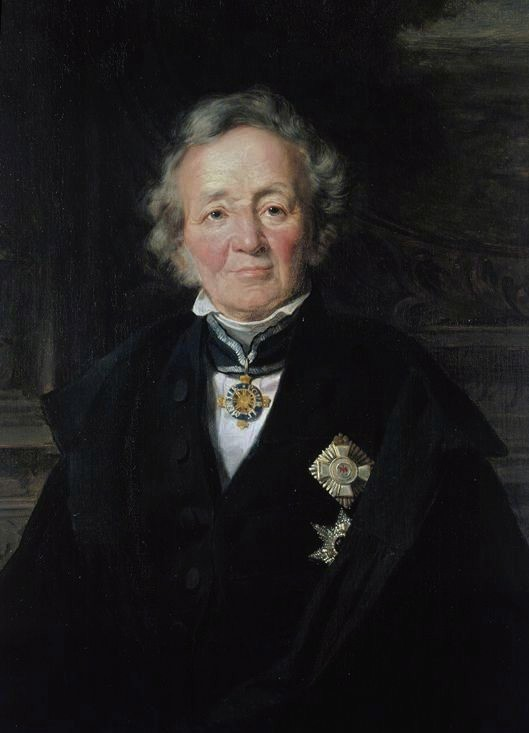
\includegraphics[width=1.0\linewidth]{../../imagens/ranke.jpg}
                \caption{Leopold Von Ranke (fonte: dom\'{i}nio p\'ublico)}
                \label{e978df58deaf86ca4da4073fca97b28afd4d3a3b}
\end{minipage}%
\hspace{0.5cm}
\end{figure}



Se o termo \textquotedbl historiador\textquotedbl  era bastante impreciso na Antiguidade (TEIXEIRA, 2008), o \textquotedbl jeito\textquotedbl  de fazer hist\'oria no s\'eculo XIX, cujo pioneirismo pode ser atribu\'{\i}do a Ranke, tem como caracter\'{\i}stica \textquotedbl o rigor metodol\'ogico do processo de investiga\c{c}\~ao\textquotedbl , assim como sua consolida\c{c}\~ao como disciplina acad\^emica (Marczal, 2016).










A ideia subjacente ao pensamento Rankeano \'e de que existe uma verdade objetiva no passado que precisa ser descoberta e descrita no presente como \textquotedbl conhecimento verdadeiro\textquotedbl , com base em vest\'{\i}gios aut\^enticos que servem para comprovar o que est\'a sendo narrado (Marczal, 2016).










Para a constru\c{c}\~ao do m\'etodo de registro hist\'orico que ser\'a utilizado neste trabalho, n\~ao negligenciaremos, mesmo sem ficar restritos a ele, o entendimento de Ranke, exposto no Pref\'acio \`a 1ª edi\c{c}\~ao de seu \textquotedbl Hist\'oria dos povos germ\^anicos e latinos\textquotedbl   (apud BENTIVOGLIO, 2010), que explicita:











\noindent\begin{center}\mbox{\centering\fbox{\centering\par\parbox{0.7\linewidth}{\small\textit{\textquotedbl [...] a origem da mat\'eria [hist\'orica] s\~ao mem\'orias, di\'arios, cartas, relatos de delega\c{c}\~oes e narra\c{c}\~oes originadas de testemunhas oculares; baseia-se em outros escritos somente quando estes foram diretamente derivados destes, ou quando pareciam terem sido tornados equivalentes a estes com base em algum conhecimento original\textquotedbl  (Fonte: Leopold von Ranke, no Pref\'acio da 1ª Edi\c{c}\~ao de \textquotedbl Hist\'oria dos povos germ\^anicos e latinos\textquotedbl , citado por  BENTIVOGLIO (2010))}\normalsize}}}\end{center}


Ranke, no mesmo texto, ainda segundo  BENTIVOGLIO (2010), exp\~oe qual seria o 2º passo da atividade de pesquisa hist\'orica: \textquotedbl (...)uma rigorosa exposi\c{c}\~ao de fatos seja esta t\~ao condicionada e desagrad\'avel quanto for \'e, sem d\'uvida, lei suprema\textquotedbl , refor\c{c}ando que \textquotedbl (...)n\~ao se pode fazer o mesmo desenvolvimento livre que, pelo menos, a teoria busca numa obra po\'etica(...)\textquotedbl .










Evidente que os m\'etodos da pesquisa em Hist\'oria evolu\'{\i}ram muito depois das contribui\c{c}\~oes de Ranke e seus colegas da Escola Hist\'orica Prussiana do s\'eculo XIX, sobretudo, pelo fato da ci\^encia  da hist\'oria se tornar o centro de oposi\c{c}\~ao ao idealismo, ensejando o surgimento de v\'arios outros movimentos historiogr\'aficos e Escolas.










Sem, contudo, adentrar ao detalhamento te\'orico-filos\'ofico-metodol\'ogico, citamos, dentre as principais correntes historiogr\'aficas, al\'em da Escola Prussiana: a Escola Met\'odica dita Positivista, o Materialismo Hist\'orico e a Escola dos Annales, que passamos a descrever.










Pode-se dizer que a Escola Met\'odica, dita Positivista, foi inspirada em Von Ranke, mas teve tamb\'em influ\^encia da corrente filos\'ofica positivista difundida pelo franc\^es Augusto Comte.










A Escola Met\'odica nasceu com a proposta de  lan\c{c}ar sobre as pesquisas em hist\'oria uma vis\~ao cient\'{\i}fica, tratando a hist\'oria como uma ci\^encia metodologicamente rigorosa, tendo como modelo as ci\^encias naturais, seguindo o m\'etodo das ci\^encias f\'{\i}sicas.










Atrav\'es da Revista Hist\'orica, seus principais representantes, Charles-Vitor Langlois e Charles Seignobos, difundiam seus pensamentos.











\noindent\begin{center}\mbox{\centering\fbox{\centering\par\parbox{0.7\linewidth}{\small\textit{\textquotedbl M\'etodo tornou-se a palavra-chave, e o que distinguia a hist\'oria da literatura. A hist\'oria se profissionalizou definitivamente numerosas cadeiras na universidade, sociedades cient\'{\i}ficas cole\c{c}\~oes de documentos, revistas, manuais, publica\c{c}\~ao de textos hist\'oricos, um p\'ublico culto comprador de livros hist\'oricos”  (REIS , 2006)}\normalsize}}}\end{center}


Assim, embora essa Escola tenha recebido justas cr\'{\i}ticas dos historiadores do s\'eculo XX, a Escola met\'odica francesa teve o m\'erito inconteste de atribuir confiabilidade ao m\'etodo hist\'orico










O Materialismo Hist\'orico e Dial\'etico, ou simplesmente Materialismo Hist\'orico, foi desenvolvido  por Karl Marx (1818-1883) e Friedrich Engels (1820-1895). Nasceu da oposi\c{c}\~ao ao idealismo e se diferencia por ser uma corrente filos\'ofica que utiliza o conceito de dial\'etica para entender a din\^amica e os processos sociais, cujo enfoque te\'orico, metodol\'ogico e anal\'{\i}tico \'e utilizado para compreender as grandes transforma\c{c}\~oes da hist\'oria e das sociedades humanas.










Para  Pires (2009), o m\'etodo materialista hist\'orico-dial\'etico “caracteriza-se pelo movimento do pensamento atrav\'es da materialidade hist\'orica da vida dos homens em sociedade, isto \'e, trata-se de descobrir (pelo movimento do pensamento) as leis fundamentais que definem a forma organizativa dos homens durante a hist\'oria da humanidade.”, sendo um paradigma que vem influenciando at\'e hoje a historiografia mundial.










Para Firat (1987), \textquotedbl a an\'alise marxista se situa entre os Annales e as tradi\c{c}\~oes hermen\^euticas\textquotedbl , alertando para o risco da interpreta\c{c}\~ao da realidade ser distorcida pelas \textquotedbl experi\^encias materiais dos seres humanos\textquotedbl .










Dando prosseguimento a esta breve e despretensiosa revis\~ao do m\'etodo historiogr\'afico, chegamos \`a Escola de Annales, cujo nome tem origem na sua forma de mobiliza\c{c}\~ao inicial, a Revista Annales: \'economies, societ\'es, civilisations, fundada em 1929, que representou uma ruptura com a vis\~ao hist\'orica tradicional (PIERANTI, 2022) .










A Escola de Annales trouxe uma nova abordagem, com in\'umeras consequ\^encias e influ\^encias at\'e nossos dias. Tem como principais mentores  Marc Bloch e Lucian Febvre.










Sobre a revista, Peter Burke (1991) afirma no Pref\'acio que esta:











\noindent\begin{center}\mbox{\centering\fbox{\centering\par\parbox{0.7\linewidth}{\small\textit{“foi fundada para promover uma nova esp\'ecie de hist\'oria e continua, ainda hoje, a encorajar inova\c{c}\~oes. As id\'eias diretrizes da revista, que criou e excitou entusiasmo em muitos leitores, na  Fran\c{c}a e no exterior, podem ser sumariadas brevemente. Em primeiro lugar, a substitui\c{c}\~ao da tradicional narrativa de acontecimentos por uma hist\'oria-problema. Em segundo lugar, a hist\'oria de todas as atividades humanas e n\~ao apenas hist\'oria pol\'{\i}tica. Em terceiro lugar, visando completar os dois primeiros objetivos, a colabora\c{c}\~ao com outras disciplinas, tais como a geografia, a sociologia, a psicologia, a economia, a lingu\'{\i}stica, a antropologia social, e tantas outras.\textquotedbl   (Burke, 1991)}\normalsize}}}\end{center}


N\~ao obstante a percep\c{c}\~ao de uma certa proximidade entre a Escola de Annales e o positivismo, quando comparada com outras tradi\c{c}\~oes na metodologia da hist\'oria, dado que ambas t\^em a abordagem pelo m\'etodo cient\'{\i}fico como dominante, sempre com \^enfase em fatos emp\'{\i}ricos (Firat, 1987), \'e evidente que na Escola de Annales a narrativa linear dos acontecimentos sai de cena (PIERANTI, 2022), dando espa\c{c}o a uma metodologia cr\'{\i}tica.










Em sua segunda fase, identificada com Fernand Braudel, a ideia fundamental era de que a hist\'oria \'e regida por fen\^omenos de longa dura\c{c}\~ao, como os que dominaram a Revolu\c{c}\~ao Francesa ou a Idade M\'edia, por exemplo. \'E justamente o estudo sobre a Revolu\c{c}\~ao Francesa, conduzido por Ernest Labrousse, que traz para dentro da Escola de Annales a dita \textquotedbl revolu\c{c}\~ao quantitativa\textquotedbl , entre os anos de 1950 e 1970  (Burke, 1991).










Este per\'{\i}odo, que \'e de maior interesse para o m\'etodo que aqui construiremos, se caracteriza pelo nascimento da Hist\'oria Quantitativa (Burke, 1991), no contexto dos estudos sobre pre\c{c}os na Fran\c{c}a do s\'eculo XVIII.










Tais estudos se caracterizavam pelos m\'etodos estat\'{\i}sticos trazidos para a Escola de Annales por Labrousse, que, por sua vez, era \textquotedbl incentivado pelos economistas Albert Aftalion e Fran\c{c}ois Simiand a empreender um rigoroso estudo quantitativo da economia francesa do s\'eculo XVIII\textquotedbl   (Burke, 1991). Esse estudo culminou em duas publica\c{c}\~oes:











\begin{alineas}
\item \textquotedbl Esquisse\textquotedbl  (1933), ou \textquotedbl Retrato Falado\textquotedbl  (em tradu\c{c}\~ao livre), sobre os movimentos de pre\c{c}os entre 1701 e 1817  (Burke, 1991)
\item La crise de l`economie fran\c{c}aise \`a la fin de l`Ancien R\'egime et au d\'ebut de la Revolution (1944), ou \textquotedbl A crise da economia francesa no final do Antigo Regime e in\'{\i}cio da Revolu\c{c}\~ao\textquotedbl  (em tradu\c{c}\~ao livre), sobre o fim do antigo regime  (Burke, 1991).

\end{alineas}

Segundo  Burke (1991), Braudel teria proclamado, em sua \'epoca, o segundo livro de Labrousse, dois anos mais velho, como \textquotedbl o maior livro de hist\'oria publicado na Fran\c{c}a nestes \'ultimos vinte e cinco anos\textquotedbl .










Ambos os livros de Labrousse se caracterizam por serem altamente t\'ecnicos, \textquotedbl saturados de gr\'aficos e tabelas\textquotedbl   (Burke, 1991), referindo-se a movimentos de longa dura\c{c}\~ao, mas com aten\c{c}\~ao a ciclos de curta dura\c{c}\~ao.










Burke (1991) refere-se a Labrousse como uma \textquotedbl emin\^encia parda dos Annales\textquotedbl , uma vez que \textquotedbl h\'a motivos para se suspeitar que houve influ\^encia de Labrousse na 2a. Edi\c{c}\~ao do cl\'assico Mediterrainn\'ee de Braudel\textquotedbl . Isso porque nessa 2a. Edi\c{c}\~ao, de 1966, surge uma maior \^enfase na dita Hist\'oria Quantitativa, com a inclus\~ao de tabelas e gr\'aficos inexistentes na primeira Edi\c{c}\~ao.










 Firat (1987) menciona a \^enfase da Escola de Annales em \textquotedbl desenvolver um conjunto de m\'etodos na coleta e an\'alise de dados hist\'oricos\textquotedbl , visando \textquotedbl trazer cientificidade e respeitabilidade para a hist\'oria\textquotedbl .










Esta auto-imagem de ci\^encia expressada pela Escola de Annales, contrasta com a vis\~ao de Popper, que tentou reduzir as tradi\c{c}\~oes historiogr\'aficas \`a tautologia, que, nesta condi\c{c}\~ao, n\~ao poderiam ser false\'aveis e, consequentemente, seriam pseudo-ci\^encia  (Firat, 1987).










Acreditamos que esse posicionamento de Popper vem sendo superados e, objetivamente, nos atrai a vis\~ao de  Kieser (1994), que traz quatro motivos principais para re-introduzir a hist\'oria nos estudos organizacionais:











\begin{alineas}
\item Estruturas e comportamentos no presente das organiza\c{c}\~oes refletem desenvolvimentos hist\'oricos que s\~ao culturalmente espec\'{\i}ficos  (Kieser, 1994, tradu\c{c}\~ao livre). Para exemplificar,  Kieser (1994) compara a forma como organiza\c{c}\~oes alem\~as e francesas se estruturam.
\item A identifica\c{c}\~ao de como as organiza\c{c}\~oes acham solu\c{c}\~oes para seus problemas ocorre, frequentemente, de forma n\~ao independente de ideologia  (Kieser, 1994, tradu\c{c}\~ao livre) . Como exemplo,  Kieser (1994) traz o papel  que tradi\c{c}\~oes de fraternidades medievais (medieval guilds) t\^em em estruturas como IBM e Hewlett Packard, mesmo considerando que s\~ao empresas que j\'a t\^em culturas organizacionais fort\'{\i}ssimas.
\item A an\'alise hist\'orica nos ensina a interpretar estruturas organizacionais existentes n\~ao como resultado de legisla\c{c}\~ao mas como resultado de decis\~oes tomadas no passado das escolhas dispon\'{\i}veis, algumas feitas de forma intencional e outras mais implicitamente  (Kieser, 1994, tradu\c{c}\~ao livre). Como exemplo,  Kieser (1994) traz que a decis\~ao por \textquotedbl terceiriza\c{c}\~ao\textquotedbl  (putting out) teve no sucesso de algumas organiza\c{c}\~oes.
\item A confronta\c{c}\~ao de teorias de mudan\c{c}a organizacional com o desenvolvimento hist\'orico submetes essas teorias a um teste mais radical do que o que teriam que passar se fossem apenas comparadas com dados de curto prazo (Kieser, 1994, tradu\c{c}\~ao livre). Como exemplo,  Kieser (1994) cita casos de ecologia das organiza\c{c}\~oes.
\end{alineas}

\subsection[Hierarquia versus heterarquia]{Hierarquia versus heterarquia}\label{Hierarquia versus heterarquia}
A hierarquia pode ser entendida como (CRUMLEY, 1995):











\noindent\begin{center}\mbox{\centering\fbox{\centering\par\parbox{0.7\linewidth}{\small\textit{\textquotedbl (...) elementos que na base de certos fatores est\~ao subordinados a outros e podem ser ordenados (ranked)\textquotedbl  (Fonte:  CRUMLEY (1995), tradu\c{c}\~ao livre)}\normalsize}}}\end{center}


Na taxonomia, o conceito de hierarquia est\'a relacionado \`a ordem das rela\c{c}\~oes do tipo \textquotedbl est\'a contido em\textquotedbl . Os subconjuntos que est\~ao contidos em outros subconjuntos t\^em hierarquia inferior. Essa no\c{c}\~ao pode ser ampliada para o conceito de \textquotedbl sistemas dentro de sistemas\textquotedbl , que estabelece uma hierarquia mais baixa para o sistema que est\'a contido em outro.










O termo heterarquia foi usado pela primeira vez, num contexto da ci\^encia moderna  (CRUMLEY, 1995), por  McCULLOCH (1945).  Nesse trabalho o autor conduziu um estudo de redes neurais disruptivo para a \'area de neuroci\^encias porque demonstrou que n\~ao existe hierarquia entre neur\^onios no c\'erebro humano, embora exista alguma forma de ordem  (CRUMLEY, 1995).










Desse trabalho original, o termo se espalhou para muitas outras \'areas, a exemplo das ci\^encias sociais, redes de computadores e teoria das organiza\c{c}\~oes  (PERLO et al., 2012). O emprego do termo em cada \'area espec\'{\i}fica tem nuances caracter\'{\i}sticas de cada \'area.










Heterarquia \'e definida por  CRUMLEY (1995) como:











\noindent\begin{center}\mbox{\centering\fbox{\centering\par\parbox{0.7\linewidth}{\small\textit{\textquotedbl (...) rela\c{c}\~ao entre elementos em que eles n\~ao est\~ao ordenados (ranked), ou quando eles t\^em o potencial de serem ordenados (ranked) em diferentes formas.\textquotedbl }\normalsize}}}\end{center}


A literatura cita, recorrentemente  (PERLO et al., 2012) (DA SILVA, 2017) , a exemplifica\c{c}\~ao de um sistema heter\'arquico a partir da experi\^encia da batalha de Midway (1942) no pac\'{\i}fico, quando a frota americana derrotou a japonesa.










Nesse epis\'odio, os americanos perderam sua nau capit\^ania (USS Yorktown) em pouco tempo de combate, obrigando uma reorganiza\c{c}\~ao do comando. Segundo Von Foerster (apud  PERLO et al. (2012)), como resposta a esta situa\c{c}\~ao, houve um movimento espont\^aneo dos v\'arios comandantes de navios americanos para que assumissem a frente das iniciativas b\'elicas, em fun\c{c}\~ao da percep\c{c}\~ao que tinham da posi\c{c}\~ao privilegiada de observa\c{c}\~ao do teatro naval, em cada momento. Como resultado dessa iniciativa de \textquotedbl quebrar a hierarquia\textquotedbl , os americanos conseguiram vencer a batalha.










N\~ao poder\'{\i}amos nos furtar de citar a defini\c{c}\~ao de heterarquia presente na Wikipedia, porque a pr\'opria forma de organiza\c{c}\~ao e produ\c{c}\~ao de conte\'udos daquela enciclop\'edia \'e considerada como um exemplo de heter\'arquia  (CASTILHO, 2008).










Segundo a Wikipedia, no verbete \textquotedbl heterarquia\textquotedbl  consta que:











\noindent\begin{center}\mbox{\centering\fbox{\centering\par\parbox{0.7\linewidth}{\small\textit{\textquotedbl Heterarquia (...), sistema onde n\~ao h\'a um controle centralizado vertical, mas predomina uma ordem consensual. \'E diferente da homoarquia, aus\^encia de centraliza\c{c}\~ao e coer\c{c}\~ao, e da hierarquia, ordem centralizada e verticalizada.\textquotedbl  (Fonte: Wikipedia)}\normalsize}}}\end{center}


 CASTILHO (2008) define a heterarquia como segue:











\noindent\begin{center}\mbox{\centering\fbox{\centering\par\parbox{0.7\linewidth}{\small\textit{\textquotedbl (a heterarquia) procura definir uma forma de trabalho coletivo onde n\~ao h\'a um superior e nem uma agenda ou m\'etodo imposto de cima para baixo, por meio de chefias hierarquizadas. No sistema heter\'arquico existe uma ordem, decidida pela maioria, ao contr\'ario da anarquia, onde n\~ao existe ordem alguma.\textquotedbl  (Fonte:  CASTILHO (2008))}\normalsize}}}\end{center}


\subsection[Governo Eletr\^onico]{Governo Eletr\^onico}\label{Governo Eletr\^onico}
Foi no s\'eculo XIX que os primeiros conceitos de programa\c{c}\~ao come\c{c}aram a ser desenvolvidos. O mec\^anico franc\^es Joseph-Marie Jacquard (1752-1854) inventou o primeiro tear automatizado, utilizando a inova\c{c}\~ao dos cart\~oes perfurados. Outros contribuintes foram Charles Baggage (1791-1871) e Ada Lovelace (1815-1852), com o desenvolvimento do conceito de m\'aquina anal\'{\i}tica, embora a m\'aquina, propriamente dita, n\~ao tenha sido efetivamente constru\'{\i}da. No entanto, mesmo assim, seus esfor\c{c}os s\~ao considerados basilares para o desenvolvimento dos primeiros computadores. Ada Lovelace foi considerada a primeira pessoa efetivamente a se valer do conceito de programa\c{c}\~ao na Hist\'oria.










O empres\'ario norte americano Herman Hollerith (1860-1929) desenvolveu um sistema capaz de computar dados. Seu desenvolvimento se deu no contexto de uma demanda de Governo. Desde 1880, o governo americano fazia o censo demogr\'afico e demorava 8 anos para contabilizar os dados. Hollerith criou uma m\'aquina capaz de computar as informa\c{c}\~oes coletadas durante o censo de 1890, tamb\'em a partir de cart\~oes perfurados, diminuindo assim o tempo de c\'alculo para apenas dois anos e meio. Esse exemplo talvez seja uma das primeiras formas de emprego de uma tecnologia digital primitiva numa atividade de governo. Mas n\~ao era uma tecnologia voltada para disponibilizar servi\c{c}os diretamente para o cidad\~ao, um conceito que veio a se concretizar muitas d\'ecadas depois.










A partir desta iniciativa, Hollerith vendeu suas m\'aquinas para governos e empresas, tendo sido, tamb\'em, um dos fundadores da IBM, hoje uma das maiores empresas de tecnologia da informa\c{c}\~ao do mundo. Dentre os \textquotedbl servi\c{c}os\textquotedbl  prestados pela IBM, lamentavelmente, est\'a o apoio ao Holocausto nazista contra judeus e outras minorias, durante o Terceiro Reich Alem\~ao  (BLACK, 2001).










Atualmente os computadores s\~ao ferramentas indispens\'aveis para o desenvolvimento do mundo e funcionamento das sociedades contempor\^aneas, bem como do conhecimento cient\'{\i}fico. Em suma, a hist\'oria da computa\c{c}\~ao e das m\'aquinas remonta a tempos antigos, que v\~ao desde as ferramentas de c\'alculo, passando pela revolu\c{c}\~ao industrial e suas tentativas de se criar computadores mec\^anicos, os computadores eletr\^onicos anal\'ogicos  (BRITANNICA, 2022), at\'e chegar \`a forma dos computadores eletr\^onicos digitais conhecidas hoje.










Como se v\^e pela hist\'oria, o uso de tecnologias da informa\c{c}\~ao e comunica\c{c}\~ao pelos governos \'e t\~ao antigo quanto a pr\'opria exist\^encia da computa\c{c}\~ao.










No Brasil, a utiliza\c{c}\~ao da tecnologia da informa\c{c}\~ao na administra\c{c}\~ao p\'ublica teve in\'{\i}cio na d\'ecada de 1960, principalmente pelas empresas estatais  (DANTAS, 1988). Uma frase bastante repetida naquela \'epoca \'e que os engenheiros brasileiros rec\'em formados tinham pouca oportunidade de fazer engenharia de fato, e suas perspectivas se restringiam a trabalhar no governo comprando equipamentos, ou trabalhar nas multinacionais, vendendo equipamentos para o Governo. Isto se dava porque o Brasil n\~ao tinha uma cultura de desenvolvimento no mundo digital e esse tipo de atividade era desestimulada pelas filiais de empresas estrangeiras. Um esfor\c{c}o muito grande foi institu\'{\i}do no pa\'{\i}s, principalmente a partir da d\'ecada de 60, para reverter essa situa\c{c}\~ao  (DANTAS, 1988). Essa iniciativa do governo permitiu a g\^enese de uma comunidade de profissionais, estabelecendo as bases para a constitui\c{c}\~ao de uma \textquotedbl cultura digital\textquotedbl  que veio a se expressar mais amplamente a partir da d\'ecada de 90.










As press\~oes internacionais por um estado \textquotedbl gerencial e empreendedor, intensificaram o movimento conhecido por reforma da gest\~ao p\'ublica (Bresser-Pereira, 2002) ou new public management (Ferlie etal., 1996). Este movimento teve como cerne a \textquotedbl busca da excel\^encia e a orienta\c{c}\~ao aos servi\c{c}os ao cidad\~ao.










Nos prim\'ordios do emprego de tecnologias digitais em atividades de governo, a men\c{c}\~ao a \textquotedbl IT in Government (\textquotedbl Tecnologia da Informa\c{c}\~ao no Governo, em tradu\c{c}\~ao livre) se referia exclusivamente ao uso da tecnologia no interior dos governos. Portanto n\~ao era uma tecnologia voltada para disponibilizar servi\c{c}os diretamente para o cidad\~ao .










A vis\~ao gerencial da d\'ecada de 90 inaugurou a ideia de um \textquotedbl governo eletr\^onico\textquotedbl  que buscava tratar o indiv\'{\i}duo como \textquotedbl cliente\textquotedbl  de servi\c{c}os de governo, ou, na melhor das hip\'oteses, como um cidad\~ao \textquotedbl pagador de impostos\textquotedbl  que recebia em troca servi\c{c}os. Esta vis\~ao, na sua g\^enese, ainda n\~ao pensava o cidad\~ao como um titular de um conjunto completo de direitos civis.










Em que pese esse in\'{\i}cio bastante vinculado \`as controversas ideologias da \'epoca, em particular \`a no\c{c}\~ao de \textquotedbl empreendedorismo de Estado\textquotedbl , h\'a que se reconhecer que tais iniciativas prepararam a sociedade para as transforma\c{c}\~oes tecnol\'ogicas vindouras, que alteraram a rela\c{c}\~ao do Estado com seus cidad\~aos.










A ideia de governo eletr\^onico difere-se de um simples uso de \textquotedbl IT in Government\textquotedbl , porque trata do acesso direto ao governo por meios digitais pelo pr\'oprio cidad\~ao, sem intermedi\'arios. Portanto, s\'o se tornou vi\'avel a partir da dissemina\c{c}\~ao em grande escala das tecnologias de informa\c{c}\~ao e comunica\c{c}\~ao.










\'E comum atribu\'{\i}rem ao advento do WebBrowser, ou seja, ao pr\'oprio advento da internet como se conhece hoje, o pioneirismo para a dissemina\c{c}\~ao das tecnologias digitais.










Mas, por justi\c{c}a hist\'orica, \'e preciso reconhecer que antes mesmo desse marco, j\'a existia na Fran\c{c}a uma tecnologia que oferecia servi\c{c}os de todo tipo para os cidad\~aos: o MINITEL  (BBC, 2012) , que no Brasil era conhecido como V\'{\i}deo Texto. Muito antes do HTML, em meados da d\'ecada de 80, o MINITEL e suas vers\~oes locais (Su\'ecia, Irlanda, \'Africa do Sul, Canad\'a, Brasil, etc) j\'a eram extensivamente usadas. Na cidade de S\~ao Paulo o v\'{\i}deo texto da Telesp chegou a ter dezenas de milhares de assinantes  (Longhi, 2009).












\captionsetup{format=plain}
\begin{figure}[max size={\textwidth}{\textheight}]

\centering


\begin{minipage}[b]{0.4\linewidth}
        \centering
                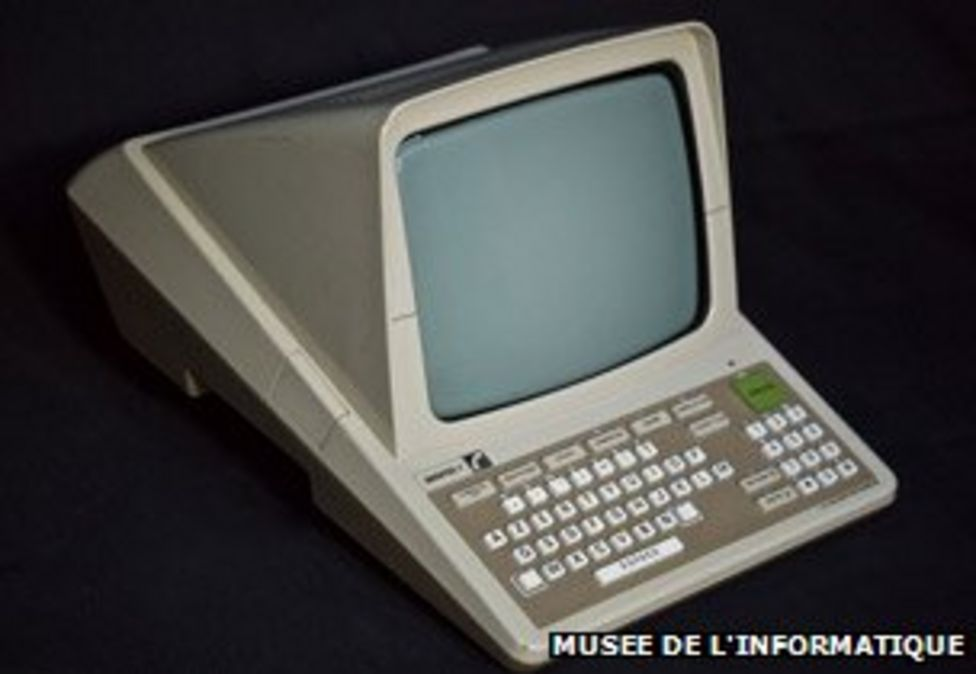
\includegraphics[width=1.0\linewidth]{../../imagens/minitel.jpg}
                \caption{Imagem de um terminal Minitel.}
                \label{5d9a2782548e094108d5241aeff768916b33be6c}
\end{minipage}%
\hspace{0.5cm}
\end{figure}



O Judici\'ario brasileiro inaugurou os servi\c{c}os digitais para atendimento ao cidad\~ao, j\'a no in\'{\i}cio da d\'ecada de noventa. Este pioneirismo se deu com o uso de c\'odigos de barra para identifica\c{c}\~ao de eleitores, por exemplo. Ali\'as, muito antes das a\c{c}\~oes do executivo, houve o desenvolvimento da Urna Eletr\^onica, uma iniciativa totalmente estatal, com a participa\c{c}\~ao de unidades de pesquisa federais  (MAMMANA et al., 1990)  (ANDRADE, 2022) . As a\c{c}\~oes do executivo brasileiro em dire\c{c}\~ao ao governo eletr\^onico remontam ao in\'{\i}cio da d\'ecada de 90, sempre com a participa\c{c}\~ao do SERPRO. Pode-se considerar que o programa de imposto de renda oferecido pela receita federal a partir de 1991 foi uma das primeiras a\c{c}\~oes em grande escala do executivo no sentido de oferta de servi\c{c}os digitais diretos para o cidad\~ao, mesmo considerando que o envio dos dados da declara\c{c}\~ao por internet s\'o foi viabilizado a partir de 1998. No in\'{\i}cio, era preciso enviar os disquetes da declara\c{c}\~ao juntamente com a documenta\c{c}\~ao em papel.










O movimento em dire\c{c}\~ao ao governo eletr\^onico ganhou mais institucionalidade a partir do final do governo FHC, principalmente com a atua\c{c}\~ao de Pedro Parente \`a frente da Casa Civil  (DINIZ, 2009).










O movimento do Brasil em dire\c{c}\~ao ao Governo Eletr\^onico se deu no contexto da j\'a mencionada tend\^encia mundial de promover Reformas Administrativas da d\'ecada de 90 e in\'{\i}cio dos anos 2000. [XXX] Ramon Garcia identificam a concomit\^ancia da a\c{c}\~ao de Brasil, M\'exico e Estados Unidos, que em 3 anos formalizaram seus programas de Governo Digital. Brasil e M\'exico focalizaram a infraestrutura da Internet, ao passo que os Estados Unidos trabalhavam para o uso da internet em servi\c{c}os e processos.










O Governo Digital no Brasil foi formalizado por Decreto Presidencial de 3 abril de 2000  (DINIZ, 2009), cuja implementa\c{c}\~ao se deu sob a coordena\c{c}\~ao pol\'{\i}tica da Presid\^encia da Rep\'ublica, com apoio t\'ecnico e gerencial da Secretaria de Log\'{\i}stica e Tecnologia da Informa\c{c}\~ao (SLTI), do Minist\'erio do Planejamento, Or\c{c}amento e Gest\~ao. Essa atua\c{c}\~ao foi sustentada por um comit\^e integrado pelos secret\'arios executivos (e cargos equivalentes) dos minist\'erios e \'org\~aos da Presid\^encia da Rep\'ublica, denominado Comit\^e Executivo de Governo Eletr\^onico (Cege).










Inicialmente o governo brasileiro concentrou esfor\c{c}os em tr\^es linhas de a\c{c}\~ao do Programa Sociedade da Informa\c{c}\~ao, institu\'{\i}do pelo Decreto no. 3.294, de 15 de dezembro de 1999 (e depois alterado por v\'arios instrumentos legais): universaliza\c{c}\~ao de servi\c{c}os, governo ao alcance de todos e infraestrutura avan\c{c}ada.










As iniciativas do Governo FHC eram principalmente acess\'{\i}veis a uma elite de cidad\~aos, uma vez que a maior parte da popula\c{c}\~ao n\~ao tinha acesso \`a internet, como se v\^e no estudo SIDRA do IBGE (apud Schmitz et al., 2021), e embora ainda n\~ao houvesse um apontamento de solu\c{c}\~oes sist\^emicas para sua universaliza\c{c}\~ao, essas iniciativas abriram o caminho institucional do Governo Eletr\^onico.












\captionsetup{format=plain}
\begin{figure}[htb]

	\begin{center}

		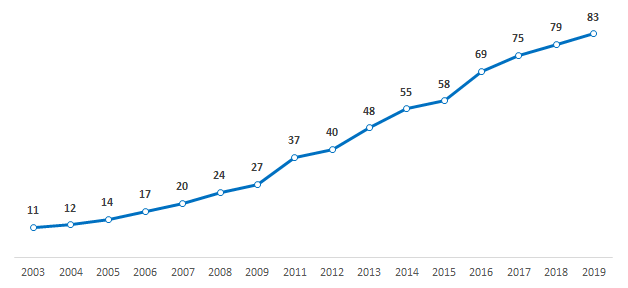
\includegraphics[max size={\textwidth}{\textheight}]{../../imagens/acesso-internet.png}

	\end{center}

	\caption{\label{dc69b8cf40fae2ba00158e43d2db2d294110957c}Evolu\c{c}\~ao do percentual de domic\'{i}lios com acesso para internet (Fonte: SIDRA 2016-2019  (apud [[Schmitz et al., 2021]]) )}

\end{figure}

\subsection[Pol\'{\i}ticas P\'ublicas de Inclus\~ao e Cultura Digital]{Pol\'{\i}ticas P\'ublicas de Inclus\~ao e Cultura Digital}\label{Pol\'{\i}ticas P\'ublicas de Inclus\~ao e Cultura Digital}
As transforma\c{c}\~oes pelas quais a sociedade passava no in\'{\i}cio dos anos 90 exigiam novos paradigmas sociais, culturais e educacionais, que envolvessem estrat\'egias de inclus\~ao dos  cidad\~aos na nova realidade.










Entretanto, esta diretriz n\~ao estava presente na fase pioneira de implanta\c{c}\~ao do governo eletr\^onico no Brasil, ainda no Governo FHC. Inicialmente, tratando os cidad\~aos como clientes, o foco era a redu\c{c}\~ao de custos unit\'arios, melhorias na gest\~ao e qualidade dos servi\c{c}os p\'ublicos, transpar\^encia governamental e simplifica\c{c}\~ao de procedimentos, formalizados como estrat\'egias, macro-objetivos e  as metas priorit\'arias  do governo brasileiro para o per\'{\i}odo de 2000 a 2003.










Paralelamente, ocorria a consolida\c{c}\~ao de uma cadeia produtiva mundial de eletro-eletr\^onicos completa e eficiente, que usufru\'{\i}a de m\~ao-de-obra barata na \'Asia. Esse fato contribuiu para a redu\c{c}\~ao de barreiras econ\^omicas para o acesso a dispositivos digitais, uma vez que houve ampla comoditiza\c{c}\~ao da produ\c{c}\~ao de eletroeletr\^onicos em geral e dos bens de computa\c{c}\~ao em particular. Esse fen\^omeno era uma decorr\^encia direta da Lei de Moore (CIPOLI, 2012), atrav\'es da qual o mundo passou a produzir mais transistores eletr\^onicos do que gr\~aos de soja, com ganhos de escala que tornaram essas tecnologias mais acess\'{\i}veis.










Apenas para registro, vale lembrar que a Lei de Moore foi observada empiricamente, pela primeira vez, por Gordon Earle Moore, presidente da fabricante de microprocessadores Intel, em 1965. Ele observou que a cada 18 meses a ind\'ustria de microchips eletr\^onicos conseguia dobrar a quantidade de transistores presentes numa pastilha de sil\'{\i}cio de \'area definida. Os transistores s\~ao os \textquotedbl tijolos\textquotedbl  da eletr\^onica e s\~ao usados para processar os sinais digitais.










Essa alta disponibilidade de equipamentos digitais, a relativo baixo custo, facilitou uma presen\c{c}a cada vez maior da internet na vida das pessoas, principalmente a partir da populariza\c{c}\~ao dos celulares do tipo \textquotedbl smart-phone\textquotedbl , situa\c{c}\~ao que se reproduziu no Brasil no in\'{\i}cio do s\'eculo XXI.










A transforma\c{c}\~ao digital estimulou os governos a enfrentarem as dificuldades  de falta de  capacita\c{c}\~ao dos cidad\~aos na apropria\c{c}\~ao tecnol\'ogica, de forma que pudessem usufruir melhor da abund\^ancia e acesso aos equipamentos digitais. Para isso, estabeleceram pol\'{\i}ticas p\'ublicas que os preparassem para usufru\'{\i}rem do direito humano \`a comunica\c{c}\~ao, como estabelecido no Art. 19 da Declara\c{c}\~ao Universal de Direitos Humanos. Ou seja, os governos passaram a se preocupar com a inser\c{c}\~ao efetiva de seus cidad\~aos na sociedade da informa\c{c}\~ao.










Essas iniciativas ficaram conhecidas, genericamente, como programas pertinentes a politicas de \textquotedbl inclus\~ao digital, ou  de \textquotedbl cultura digital\textquotedbl  ou mesmo de \textquotedbl alfabetiza\c{c}\~ao tecnol\'ogica\textquotedbl . Independentemente da abordagem escolhida, dentre as tr\^es indicadas, essas pol\'{\i}ticas sempre estiveram vinculadas \`as estruturas de educa\c{c}\~ao, seja a formal, ou a n\~ao-formal.










Diferentes iniciativas e perspectivas foram implementadas para uso das tecnologias da informa\c{c}\~ao e comunica\c{c}\~ao no Brasil na primeira d\'ecada deste s\'eculo, principalmente ao longo do primeiro e segundo mandato de Lula. Por meio de diferentes pol\'{\i}ticas p\'ublicas, foram disponibilizados, ou foi facilitado, acesso, equipamentos, aplicativos, softwares, hardwares, os quais visavam processar, armazenar, comunicar, prover apropria\c{c}\~ao tecnol\'ogica e acesso a  informa\c{c}\~ao, bem como ao conhecimento.










Dentre as pol\'{\i}ticas de inclus\~ao digital do per\'{\i}odo, destaca-se o ProInfo, pol\'{\i}tica de implanta\c{c}\~ao de \textquotedbl laborat\'orios de microcomputadores\textquotedbl  em escolas p\'ublicas, iniciada no Governo FHC e substancialmente ampliada no Governo Lula.










Tamb\'em destacam-se as pol\'{\i}ticas com vi\'es industrial voltadas para a redu\c{c}\~ao de pre\c{c}o dos computadores para consumidores finais, concomitantemente com a ado\c{c}\~ao de Software Livre, a exemplo do PC Conectado e o Computador para Todos.










A dissemina\c{c}\~ao de Telecentros tamb\'em teve um papel importante, criando pontos de acesso coletivo, que usufru\'{\i}am do GESAC, quando necess\'ario.










Para garantir a objetividade da an\'alise no contexto desta disserta\c{c}\~ao, h\'a que se concentrar nos aspectos pertinentes ao objeto de estudo, i.e. o Programa WASH. Esta restri\c{c}\~ao exige focalizar a rela\c{c}\~ao entre as tecnologias digitais e a educa\c{c}\~ao formal e n\~ao-formal, abordagens adotadas pelo projeto Workshop Aficionados por Software e Hardware-WASH, como se ver\'a mais adiante.










Assim, no esp\'{\i}rito de manter a objetividade, e por sua rela\c{c}\~ao direta na g\^enese do Programa WASH, optou-se por focalizar, neste estudo:











\begin{alineas}
\item a pol\'{\i}tica p\'ublica \textquotedbl Governo Eletr\^onico de Servi\c{c}os de Atendimento ao Cidad\~ao-GESAC\textquotedbl , programa do Minist\'erio das Comunica\c{c}\~oes, cujo o formato de interesse para este trabalho \'e o que se consolidou a partir de 2003.
\item o Programa de Inclus\~ao Digital da Secretaria de Inclus\~ao Digital do Minist\'erio de Ci\^encia e Tecnologia
\item o Projeto Um Computador por Aluno, resultado da tropicaliza\c{c}\~ao da proposta americana \textquotedbl One Laptop per Child\textquotedbl 
\end{alineas}

Tivemos um papel na constru\c{c}\~ao e execu\c{c}\~ao de pol\'{\i}ticas p\'ublicas com as caracter\'{\i}sticas acima, inicialmente no \^ambito do Governo Eletr\^onico, passando pelas \'areas de comunica\c{c}\~ao, sa\'ude, cultura, e culminando na \'area de ci\^encia e tecnologia.










Estas labora\c{c}\~oes  se deram em v\'arios momentos de nossa carreira, ao longo de quase 3 d\'ecadas. Isso nos transformou em testemunhas oculares dos fatos a elas relacionados, inicialmente no  munic\'{\i}pio de Campinas, na d\'ecada de 90, e, em seguida, no \^ambito do Governo Federal, nas primeiras duas d\'ecadas do presente s\'eculo.










Nessa trajet\'oria nos foi poss\'{\i}vel aprender sobre as vantagens e desvantagens de cada uma das abordagens adotadas ao longo dessas 3 d\'ecadas, bem como sobre a forma de combinar capacita\c{c}\~ao e estabelecimento de infraestrutura para o acesso do cidad\~ao ao mundo digital.










A partir de uma pr\'atica regular e frequente de oficinas de forma\c{c}\~ao para  crian\c{c}as e adolescentes, que se iniciou em setembro de 2013 no Centro de Tecnologia da Informa\c{c}\~ao CTI - Renato Archer em Campinas, esse aprendizado se consolidou em um m\'etodo do qual a candidata \'e co-autora, conhecido como WASH (Workshop de Aficionados em Software e Hardware).










Ap\'os um longo per\'{\i}odo de matura\c{c}\~ao, ajustes e repeti\c{c}\~ao, esse m\'etodo veio a ser formalizado em 2018 por meio de portaria de uma unidade de pesquisa do Minist\'erio da Ci\^encia, Tecnologia e Inova\c{c}\~oes (Portaria 178/2018 SEI/CTI).










A descri\c{c}\~ao detalhada do m\'etodo consta como anexo da referida portaria, a qual sintetiza os aprendizados conquistados ao longo dos anos, pelos v\'arios participantes do programa. De 2018 para c\'a, mais aprendizados ocorreram, havendo uma necessidade de aprimoramento de sua caracteriza\c{c}\~ao.










\'E justamente uma an\'alise sobre esse m\'etodo que a presente disserta\c{c}\~ao intenciona oferecer, complementada por uma proposta de melhoria, na forma de produto tecnol\'ogico, como parte dos requisitos para obten\c{c}\~ao do t\'{\i}tulo de mestre no \^ambito do mestrado profissional em ensino de ci\^encias humanas, sociais e da natureza da Universidade  Tecnol\'ogico  Federal do Paran\'a - UTFPR- Campus Londrina/PR.










\subsection[O pensamento de Papert]{O pensamento de Papert}\label{O pensamento de Papert}
Pela import\^ancia do pensamento de Papert para o Projeto One Laptop per Child (OLPC) e, portanto, para a g\^enese do WASH, cabe uma revis\~ao r\'apida de sua obra e contribui\c{c}\~oes, permitindo uma melhor compreens\~ao da inser\c{c}\~ao do WASH no universo conceitual das correntes pedag\'ogicas. Essa rela\c{c}\~ao entre a g\^enese do WASH e a proposta do OLPC ficar\'a mais clara no cap\'{\i}tulo de Resultados e An\'alise, quando hist\'oria do WASH ser\'a apresentada. Por ora, \'e oportuno restringirmo-nos \`a revisita\c{c}\~ao das contribui\c{c}\~oes de Papert.










Para conhecer  o pensamento, um pouco da hist\'oria de Papert e  a filosofia do LOGO, \'e preciso fazer uma viagem no tempo, retornando a meados da d\'ecada de 60, quando o matem\'atico e educador sul-africano, radicado nos EUA, Seymour Papert, em colabora\c{c}\~ao com outros pesquisadores, desenvolveu a linguagem  de programa\c{c}\~ao LOGO.  Foi um dos fundadores do Media Lab e diretor do grupo de Epistemologia e Aprendizado do Massachusetts Institute of Technology-MIT.










Vale ressaltar para os nativos digitais, pessoas que nasceram a partir dos anos 80 e que cresceram com essas tecnologias, que no in\'{\i}cio da era da computa\c{c}\~ao, nos anos 60, os computadores existentes eram gigantes e ocupavam andares de pr\'edios. Eram usados, apenas, por grandes empresas e governos e n\~ao se cogitava aplic\'a-los para o uso pessoal e dom\'estico. Poucas pessoas, com treinamento, conseguiam usar um computador. O mouse, por exemplo, nem existia ainda. Para entrar com informa\c{c}\~oes nos computadores, era preciso usar cart\~oes perfurados inspirados nos que foram criados pelo mec\^anico franc\^es Joseph-Marie Jacquard (1752-1854), que tamb\'em inventou o primeiro tear automatizado, cujos padr\~oes eram definidos nos cart\~oes perfurados.










Papert foi um pensador vision\'ario. Percebeu o potencial do uso da tecnologia na educa\c{c}\~ao; fil\'osofo e pioneiro no pensar o processo de aprendizagem de crian\c{c}as, de forma diferente. Em 1968, escreveu o artigo \textquotedbl Teaching Children Thinking\textquotedbl , no qual abordou a tem\'atica crian\c{c}as, educa\c{c}\~ao e computadores:











\noindent\begin{center}\mbox{\centering\fbox{\centering\par\parbox{0.7\linewidth}{\small\textit{\textquotedbl T\'{\i}nhamos a certeza de que, quando os computadores se Tornassem t\~ao comuns quanto o l\'apis, a educa\c{c}\~ao mudaria t\~ao r\'apida e profundamente quanto as transforma\c{c}\~oes pelas quais viv\'{\i}amos nos direitos civis e nas rela\c{c}\~oes sociais e sexuais\textquotedbl . [XXX colocar a cita\c{c}\~ao aqui]}\normalsize}}}\end{center}


Ele formulou esse pensamento quando os computadores dos anos 70 eram inacess\'{\i}veis tamb\'em para o sistema educacional. Naquele tempo, n\~ao existia o conceito de \textquotedbl microcomputadores\textquotedbl  e os computadores existentes eram poucos, grandes, espalhados  (SOLOMON et al., 2020) e desajeitados, com poder de processamento e armazenagem entre milhares e milh\~oes de vezes inferiores ao de um notebook de hoje. Mesmo com esse baixo desempenho, os custos eram muito altos e, portanto, o acesso era muito restrito. Entretanto, valendo-se de mainframes centralizados (computadores de grande porte) com as limita\c{c}\~oes indicadas, foi poss\'{\i}vel a Papert realizar incurs\~oes pioneiras no campo da aprendizagem para crian\c{c}as, utilizando os computadores que estavam dispon\'{\i}veis, ainda que esse uso estivesse restrito a uma elite, sem, a possibilidade de uma grande dissemina\c{c}\~ao no sistema educacional.










Toda uma gera\c{c}\~ao de educadores foi formada em torno das ideias de Papert, que defendia que a aprendizagem de linguagem de programa\c{c}\~ao de computadores, j\'a no ensino fundamental, poderia ter um papel importante no aprendizado de muitas outras disciplinas tradicionais, principalmente a matem\'atica, mas tamb\'em gram\'atica (SOLOMON et al., 2020), entre outras.










Entendemos que a proposta de Papert, at\'e por enfatizar o aprendizado de crian\c{c}as, n\~ao tinha qualquer ambi\c{c}\~ao de capacita\c{c}\~ao profissional e, por si s\'o, n\~ao visava diretamente fazer frente aos desafios do \textquotedbl mundo do trabalho\textquotedbl , que foram sendo introduzidos pelas transforma\c{c}\~oes inerentes \`a Sociedade da Informa\c{c}\~ao, nas d\'ecadas subsequentes.










Em sua obra \textquotedbl A M\'aquina das Crian\c{c}as\textquotedbl  (1994), Papert discorre sobre a import\^ancia da tecnologia e sua inser\c{c}\~ao na educa\c{c}\~ao, a fim de melhorar a qualidade do ambiente de aprendizagem.











\noindent\begin{center}\mbox{\centering\fbox{\centering\par\parbox{0.7\linewidth}{\small\textit{N\'os podemos dar um poder sem precedentes para as crian\c{c}as inventarem e desenvolverem projetos excitantes, provendo o acesso a computadores, com uma linguagem de programa\c{c}\~ao adequada, intelig\'{\i}vel e clara, bem como com perif\'ericos capazes de produzir uma a\c{c}\~ao on-line/real-time\textquotedbl   (SOLOMON et al., 2020)}\normalsize}}}\end{center}


Segundo o autor, \textquotedbl ao redor do mundo inteiro, as crian\c{c}as entraram em um apaixonante e duradouro caso de amor com os computadores\textquotedbl  (1994, p.07).










Essa filosofia e maneira de colocar em pr\'atica a crian\c{c}a epistem\'ologa vieram do seu aprendizado na rela\c{c}\~ao de trabalho e conviv\^encia com Piaget.










Papert ficou impressionado de ver as crian\c{c}as, construtoras de suas pr\'oprias estruturas intelectuais [Logo, computadores e educa\c{c}\~ao, p\'ag 35]:











\noindent\begin{center}\mbox{\centering\fbox{\centering\par\parbox{0.7\linewidth}{\small\textit{A linguagem LOGO faz com que o computador deixe de ser apenas um meio de transferir informa\c{c}\~ao e passe a ser a ferramenta, com a qual a crian\c{c}a pode formalizar os seus conhecimentos intuitivos. (XXX)}\normalsize}}}\end{center}


Essa nova rela\c{c}\~ao com a computa\c{c}\~ao, proposta por Papert, permitiu uma transforma\c{c}\~ao na educa\c{c}\~ao e no processo de ensino e aprendizagem, colocando o computador como relevante para o ensino fundamental, mas sempre entendendo a crian\c{c}a como programadora e n\~ao apenas como usu\'aria.










Papert examinou as crian\c{c}as que tinham aprendido a programar computadores e identificou que elas podiam usar os modelos concretos para \textquotedbl pensar sobre o pensar\textquotedbl  e \textquotedbl aprender sobre o aprender\textquotedbl  [XXX], estimulando-as  a aumentarem seus poderes de epistem\'ologos. Sobre isso, ele discorreu no artigo publicado, em 1970, intitulado Teaching Children Thinking.










Segundo Jos\'e Armando Valente, um dos respons\'aveis, em conjunto com a Professora Afira Vianna Ripper, pela tradu\c{c}\~ao do livro LOGO: computadores e educa\c{c}\~ao: \textquotedbl Papert acreditava que o computador era a ferramenta que propiciava \`as crian\c{c}as as condi\c{c}\~oes de entrar em contato com algumas das mais profundas ideias em ci\^encia, matem\'atica, e a cria\c{c}\~ao de modelos\textquotedbl .










Programar, na filosofia LOGO, significa \textquotedbl comunicar-se com o computador, numa linguagem que tanto ele, quanto o homem,  podem entender\textquotedbl . Toda crian\c{c}a aprende a falar. Por que, ent\~ao, n\~ao deveria aprender a \textquotedbl falar\textquotedbl  com um computador?\textquotedbl  Indagava Papert [XXX].










A proposta de Papert envolvia, tamb\'em, a ideia de que o computador pudesse ser um interlocutor  de matem\'atica ou um interlocutor de l\'{\i}nguas. Nessa concep\c{c}\~ao, o LOGO, ao ser um interlocutor da matem\'atica, contribui, de uma maneira l\'udica, para superar as barreiras matof\'obicas (fobia por matem\'atica e fobia pelo aprendizado [XXX]), transformando a matem\'atica, que passa a ser uma l\'{\i}ngua viva [XXX].










Papert abordou sobre a \textquotedbl matofobia: o medo de aprender\textquotedbl , com duas associa\c{c}\~oes: o conhecido medo da matem\'atica, que tem a intensidade de uma verdadeira fobia; e o  significado do radical mathe, que, em grego, significa aprender.











\noindent\begin{center}\mbox{\centering\fbox{\centering\par\parbox{0.7\linewidth}{\small\textit{\textquotedbl A matofobia pode cultural e materialmente limitar a vida das pessoas. Muitas outras pessoas ainda n\~ao desistiram completamente de aprender, mas sentem-se impedidas por opini\~oes negativas, arraigadas sobre suas capacidades. A defici\^encia torna-se uma identidade, \textquotedbl n\~ao consigo aprender franc\^es, n\~ao tenho ouvido para l\'{\i}nguas, nunca poderia ser um homem de neg\'ocios, n\~ao tenho cabe\c{c}a para contas. Essas cren\c{c}as s\~ao supersti\c{c}\~oes e est\~ao presentes em nosso cotidiano, elas criam tabus para a aprendizagem. Se as pessoas acreditam que n\~ao podem entender matem\'atica, conseguiram abster-se de tentar executar qualquer coisa que reconhe\c{c}am a matem\'atica, gerando como consequ\^encia uma auto-sabotagem\textquotedbl   [LOGO: Computadores e educa\c{c}\~ao, PAPERT, S. pg.62, 63]}\normalsize}}}\end{center}


Papert chamou aten\c{c}\~ao quanto \`a separa\c{c}\~ao, imposta por nossa cultura, entre o verbal e o matem\'atico. Tornou-se muito comum falar como se houvesse diferentes c\'erebros ou mesmo \'org\~aos separados no c\'erebro, para matem\'atica e linguagem.










Em suas viv\^encias com as crian\c{c}as, Papert materializava o pensamento abstrato da matem\'atica. Ao constru\'{\i}rem os seus jogos, primeiro, as crian\c{c}as faziam o movimento com o seu corpo, para, depois, usar os comandos do LOGO. A ilustra\c{c}\~ao deste processo pode ser vista no v\'{\i}deo  da entrevista, realizada com a Professora Afira Ripper,  um dos produtos desta disserta\c{c}\~ao (ver no cap\'{\i}tulo de Produtos Tecnol\'ogicos).










As crian\c{c}as s\~ao permeadas por ideias de que h\'a pessoas boas em matem\'atica e outras que n\~ao podem entender matem\'atica; mas, Papert acreditava que a presen\c{c}a do computador poderia neutralizar a matofobia [XXX].










Papert criticou os modos como os computadores estavam sendo usados na educa\c{c}\~ao americana [XXX], ou seja, como m\'aquinas, para fornecer informa\c{c}\~oes ou instrumentos de instru\c{c}\~ao assistida por computador (CAI – Computed Aid instruction)  (PAPERT, 2005a).










Segunda a percep\c{c}\~ao do autor, o tipo de abordagem existente materializava a ideia do computador programando a crian\c{c}a [XXX]. O LOGO, enquanto linguagem de programa\c{c}\~ao pensada para as crian\c{c}as, tinha como proposta inverter essa rela\c{c}\~ao.










Papert p\^ode conferir, com as crian\c{c}as em idade pr\'e-escolar, que \'e poss\'{\i}vel ela controlar a m\'aquina e ser protagonista na programa\c{c}\~ao do seu computador. Com isso, ao ensinar o computador a pensar, ela explora a sua pr\'opria forma de pensar.










Teaching Children Thinking, artigo escrito por Papert, foi a primeira publica\c{c}\~ao que sugeria que a crian\c{c}a poderia ficar no comando da m\'aquina e n\~ao a m\'aquina no comando da crian\c{c}a.  Esse artigo  foi publicado em 1970; e,  apresentou um novo processo para a educa\c{c}\~ao, em que os computadores pudessem serem usados para a criatividade.










Papert apresentou uma nova ideia: de que \textquotedbl ensinar o pensamento\textquotedbl   \'e apropriado para a escola prim\'aria, mas essa n\~ao era a corrente principal da educa\c{c}\~ao americana, naquele contexto.










O LOGO segundo Papert,  proporcionou a milhares de professores do ensino b\'asico a sua primeira oportunidade para apropriar-se do computador, de maneira que ampliaram seus estilos pessoais de ensinar. ( Papert, S, \textquotedbl A maquina das crian\c{c}as, repensando a escola da era da inform\'atica\textquotedbl  , pg57).










Em seu percurso de pesquisa, na apresenta\c{c}\~ao do LOGO, na experimenta\c{c}\~ao, seja com as crian\c{c}as ou com os professores, Papert encontrou o que ele chamava de \textquotedbl professores conservadores e  inovadores\textquotedbl  [XXX].










Outro aspecto importante na obra e viv\^encia de Papert \'e quanto aos modos hier\'arquicos de pensar sobre o conhecimento.  Ele adotou o termo  \textquotedbl heterarquia\textquotedbl  para descrever a forma de aprendizagem pretendida, um conceito presente em  \textquotedbl A m\'aquina das Crian\c{c}as\textquotedbl . Trata-se de  um termo oposto \`a hierarquia, comum na forma de trabalho da escola tradicional. Como vimos na se\c{c}\~ao XXX, na heterarquia, cada elemento \'e igualmente governado por todos os outros.










Mais adiante ser\'a poss\'{\i}vel mostrar que o WASH se estruturou numa forma de heterarquia, assunto que ser\'a tratado nos resultados.










A proposta de Papert para o Governo Federal, em 2005, n\~ao foi a primeira oportunidade de intera\c{c}\~ao com o poder p\'ublico brasileiro.










Em 1989, quando a prefeita eleita Luiza Erundina de Souza assumiu a Prefeitura de S\~ao Paulo, convidou o Prof. Paulo Freire para assumir a pasta de educa\c{c}\~ao. Um novo projeto pol\'{\i}tico-educacional foi elaborado a partir de uma reavalia\c{c}\~ao dos existentes. A partir dessa iniciativa, foi recriado o projeto de Educa\c{c}\~ao e Inform\'atica da Secretaria Municipal de Educa\c{c}\~ao de S\~ao Paulo, fundamentando-se na tese de que:











\noindent\begin{center}\mbox{\centering\fbox{\centering\par\parbox{0.7\linewidth}{\small\textit{[…] uma sociedade informatizada est\'a passando a exigir homens com potencial de assimilar a \textquotedbl novidade\textquotedbl  e criar o novo, o homem aberto para o mundo, no sentido que lhe confere a teoria piagetiana quando se refere \`as assimila\c{c}\~oes mentais majorantes; da mesma forma, exige a presen\c{c}a do cidad\~ao cr\'{\i}tico e comunit\'ario, onde os artefatos tecnol\'ogicos, especificamente o computador, possam ser ferramentas auxiliares para a constru\c{c}\~ao de uma sociedade mais igualit\'aria e justa. (S\~AO PAULO, 1992 , p. 7).Em 1995 Paulo Freire}\normalsize}}}\end{center}


Ao longo da consolida\c{c}\~ao dos conceitos descritos at\'e aqui, Papert estabeleceu uma vertente do construcionismo com grandes resultados pr\'aticos, tendo inaugurado a base para uma cultura de aprendizagem baseada no \textquotedbl fazer\textquotedbl , sustentada em ideias como:











\begin{alineas}
\item A crian\c{c}a deve estar no centro do processo de aprendizagem, conduzindo-o sempre que poss\'{\i}vel
\item N\~ao existe idade ideal para aprender as coisas: cada crian\c{c}a tem o seu pr\'oprio tempo e momento de interesse
\item Das pr\'oprias palavras de Papert: \textquotedbl a meta \'e ensinar de forma a produzir a maior aprendizagem a partir do m\'{\i}nimo de ensino\textquotedbl   (PAPERT, 1994)
\end{alineas}

Com estes conceitos, Papert indica a necessidade de estimular as crian\c{c}as a fazerem suas pr\'oprias pescarias  (PAPERT, 1994) com vistas a obter o conhecimento.










Complementam essas ideias, os conceitos de  (PAPERT, 1999):











\begin{alineas}
\item Learn by doing, ou aprender fazendo: a ideia, em parte senso comum em parte originada por Dewey, \'e aprender ao longo do processo de fazer coisas que realmente nos causa interesse
\item Technology as a building material, ou \textquotedbl tecnologia como um material de constru\c{c}\~ao\textquotedbl : a tecnologia nos permite fazer muito mais \`a medida que aprendemos, porque ela nos empodera, com seus recursos, para alcan\c{c}ar caracter\'{\i}sticas em nossas produ\c{c}\~oes, seja um jogo, prot\'otipo ou pe\c{c}a de comunica\c{c}\~ao, por exemplo, que n\~ao conseguir\'{\i}amos sem ela.
\item Hard fun, ou \textquotedbl divers\~ao desafiadora\textquotedbl : existe um entendimento de que aprende-se melhor quando nos divertimos, mas a divers\~ao n\~ao requer que a atividade seja f\'acil. \'E preciso garantir que a aprendizagem, mesmo sendo divertida, tenha um car\'ater de desafio que instigue o educando.
\item Learn to learn, ou \textquotedbl aprenda a aprender\textquotedbl : o conceito subjacente \'e o de protagonismo do educando na aprendizagem, implicando que a ideia de ensinar \'e muito menos importante do que a ideia de aprender.
\item Taking time, ou \textquotedbl assumindo o controle do seu pr\'oprio tempo\textquotedbl : os estudantes devem, ao assumir o protagonismo de sua aprendizagem, gerenciar o pr\'oprio tempo e suas pr\'oprias atividades, sem a necessidade de algu\'em lhes dizendo o que fazer
\item You can't get it right without getting it wrong, ou \textquotedbl voc\^e n\~ao consegue acertar se n\~ao errar primeiro\textquotedbl : \'e o conceito de que para aprender \'e precisa existir a liberdade para errar. As coisas importantes nunca funcionam da primeira vez, e ao tentar corrig\'{\i}-las \'e que o processo de aprendizagem ocorre
\item Do unto ourselves what we do unto our students, ou \textquotedbl fa\c{c}amos conosco o que fazemos com nossos estudantes\textquotedbl : este conceito \'e direcionado aos educadores, que precisam adotar para si a ideia de que tamb\'em v\~ao aprender fazendo e tamb\'em v\~ao aprender errando. A melhor li\c{c}\~ao para nossos estudantes \'e deix\'a-los nos assistir \textquotedbl sofrendo\textquotedbl  durante o nosso pr\'oprio aprendizado
\item We are entering a digital world, ou \textquotedbl n\'os estamos entrando em um mundo digital\textquotedbl : conhecer e saber atuar dentro do mundo digital \'e t\~ao importante quando ler ou escrever.
\end{alineas}

Mitchel Resnick, do Grupo Lifelong Kindergarten, MIT, baseado nas ideias construcionistas de Seymour Papert, apresenta, em 2007, o Scratch, como uma ferramenta para a aprendizagem criativa, considerando os 4 Ps da aprendizagem criativa: projetos, paix\~ao, pares e pensar brincando (play). A iniciativa de Resnick se consolidou. \'E por isso que, hoje, voc\^e pode encontrar no Scratch um aliado no processo de aprendizagem. O Scratch re\'une uma comunidade ativa, da qual fazem parte quase 50 milh\~oes de crian\c{c}as, jovens e adultos do mundo inteiro. O Coordenador do Programa WASH teve a oportunidade de conhecer uma das primeiras vers\~oes do Scratch, descrita pessoalmente pelo Prof. Resnick, naquela \'epoca.










O Programa WASH, seguindo nossa hip\'otese de que tem g\^enese nas propostas do OLPC, se inspirou na metodologia subjacente ao Scratch e, desde os prim\'ordios, tem como base o uso desse instrumento nas atividades de educa\c{c}\~ao. O WASH estimula a cultura digital no turno e contraturno escolares e oferece oficinas, que n\~ao podem ser classificadas como aulas tradicionais, porque abdicam de roteiros, apostilas e conte\'udos fixos, uma caracter\'{\i}stica muito presente nos m\'etodos criados pelos pensadores do MIT, disc\'{\i}pulos de Papert. Nessa concep\c{c}\~ao, o educando aprende, fazendo e errando, com objetivos determinados e oportunidade para tentar de novo. Assim, embora haja uma abertura muito grande para a experimenta\c{c}\~ao de propostas variadas, o Programa WASH oferece, como linha b\'asica de a\c{c}\~ao, a programa\c{c}\~ao de jogos usando a linguagem Scratch, e isto ser\'a visto adiante.










Ao usar o Scratch, nas oficinas do Programa WASH, estamos oportunizando e estimulando \textquotedbl as crian\c{c}as e jovens a serem criativas, produzirem seus jogos, suas narrativas, suas anima\c{c}\~oes, o racioc\'{\i}nio l\'ogico, contribuindo com o letramento digital, colaborando com a alfabetiza\c{c}\~ao cient\'{\i}fica, e para n\~ao serem somente consumidores de jogos, games, mas produtores, tamb\'em\textquotedbl .










Os resultados do emprego do Scratch no Programa WASH ser\~ao discutidos em Resultados e An\'alise, mas pode-se antecipar que envolveram milhares de crian\c{c}as e jovens produzindo jogos, com os bolsistas de inicia\c{c}\~ao cient\'{\i}fica aprendendo com o ensinar, multiplicando e compartilhando o conhecimento das ferramentas digitais  com a comunidade, tanto por meio das oficinas do WASH, quanto pela participa\c{c}\~ao em feiras, eventos e congressos.










Em nossa viv\^encia, a tartaruga, de Seymour Papert; e o gato, de Mitchel Resnick,  representam as bases da  programa\c{c}\~ao e com eles aprendemos a  programar,  brincando.










\subsection[O LOGO e o SCRATCH]{O LOGO e o SCRATCH}\label{O LOGO e o SCRATCH}
O LOGO \'e uma linguagem de programa\c{c}\~ao desenvolvida em 1966 por Seymour Papert, Wallace Feurzeig, Daniel Bobrow e Cynthia Solomon, no \^ambito dos laborat\'orios Bolt, Beranek and Newman, Inc (BBN) and MIT Artificial Intelligence Lab (SOLOMON et al., 2020). O LOGO foi muito difundido no contexto educacional a partir daquela d\'ecada, tendo ajudado gera\c{c}\~oes de crian\c{c}as a aprender v\'arias disciplinas, mas principalmente matem\'atica  (SOLOMON et al., 2020) .












\captionsetup{format=plain}
\begin{figure}[max size={\textwidth}{\textheight}]

\centering


\begin{minipage}[b]{0.4\linewidth}
        \centering
                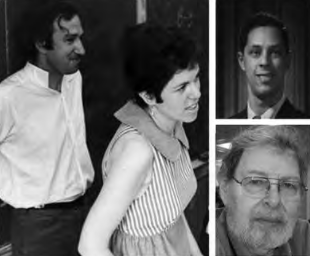
\includegraphics[width=1.0\linewidth]{../../imagens/criadores-logo.png}
                \caption{Criadores do Logo em 1966: Seymour Papert, Cynthia Solomon, Danny Bobrow e Wally Feurzeig (fonte:  [[SOLOMON et al. (2020)]])}
                \label{c40acbbf355efda753f44d02f297bbce67f5e4b8}
\end{minipage}%
\hspace{0.5cm}
\begin{minipage}[b]{0.4\linewidth}
        \centering
                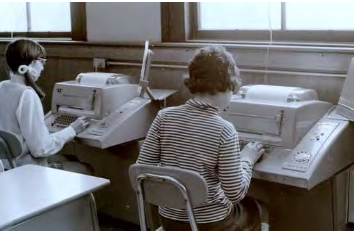
\includegraphics[width=1.0\linewidth]{../../imagens/criancas-1968.png}
                \caption{Crian\c{c}as de 12 anos da Muzzey Junior High School usando LOGO em terminais teletipo (Fonte:  [[SOLOMON et al. (2020)]], circa 1968).}
                \label{1a5368da06f895c87008b3fc1675ccfbb494f1f9}
\end{minipage}
\hspace{0.5cm}
\begin{minipage}[b]{0.4\linewidth}
        \centering
                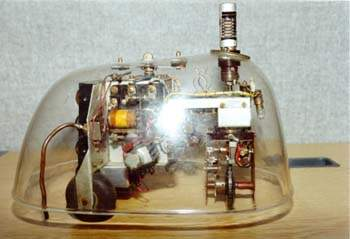
\includegraphics[width=1.0\linewidth]{../../imagens/Elmer-Elsie4.jpg}
                \caption{Elmer e Elsie eram dois rob\^os com rodas, chamados de c\'agados (tortoise), que podiam se deslocar pelo ch\~ao. Foram desenvolvidos pelo Ingl\^es Grey Walter.}
                \label{fdc1f0b8e99c3e3a345c88c79ff4e953d65b3424}
\end{minipage}%
\hspace{0.5cm}
\begin{minipage}[b]{0.4\linewidth}
        \centering
                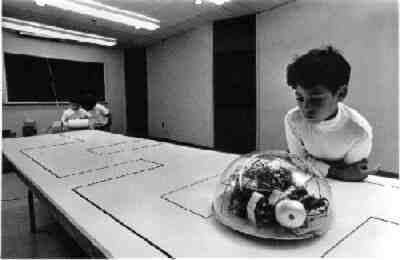
\includegraphics[width=1.0\linewidth]{../../imagens/historia-logo-turtle-01.jpg}
                \caption{Em foto de 1969, uma crian\c{c}a observa o primeiro rob\^o tartaruga criado no MIT (Fonte:  [[CIBERNECTZOO (2010)]]).}
                \label{c2ca828982a83621e08977a23628db7b32a934d9}
\end{minipage}
\hspace{0.5cm}
\begin{minipage}[b]{0.4\linewidth}
        \centering
                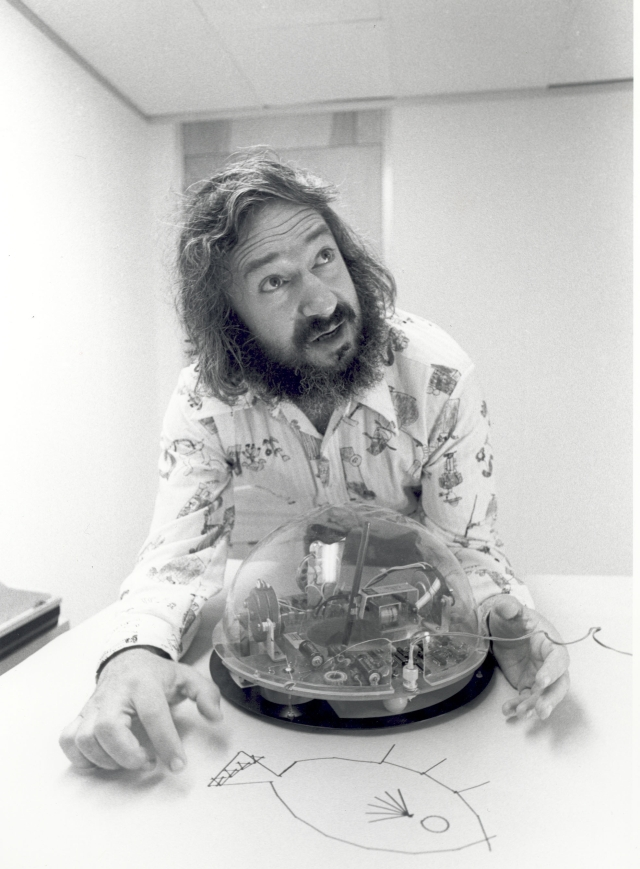
\includegraphics[width=1.0\linewidth]{../../imagens/Papert-x640.jpg}
                \caption{Papert com uma de suas tartarugas rob\^os. (Fonte:  [[CIBERNECTZOO (2010)]])}
                \label{16372e5cf76e6860245131e51a3bf17c58dd1e46}
\end{minipage}%
\hspace{0.5cm}
\begin{minipage}[b]{0.4\linewidth}
        \centering
                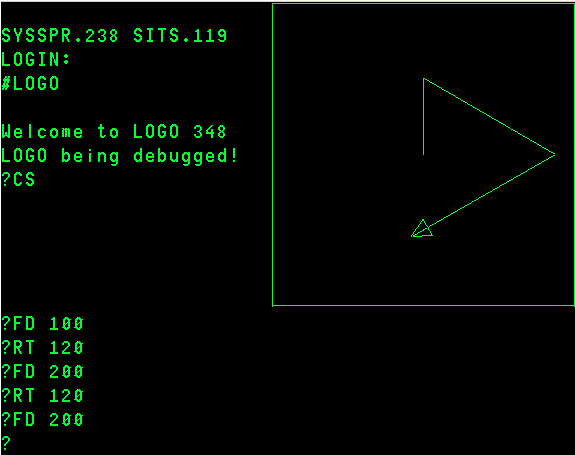
\includegraphics[width=1.0\linewidth]{../../imagens/logo-PDP11.png}
                \caption{Imagem de uma tela do LOGO num terminal gr\'afico da d\'ecada de 70, provavelmente rodando em um PDP11. O tri\^angulo pequeno \'e a tartaruga (Fonte: gunkies.org).}
                \label{ca83b217b58f57e503ff496c6c6f47bee5dc77cd}
\end{minipage}
\hspace{0.5cm}
\end{figure}



No LOGO, a constru\c{c}\~ao se d\'a pela cria\c{c}\~ao, jun\c{c}\~ao e reaproveitamento de algoritmos de computador, como num jogo de encaixe.










O LOGO possibilita a defini\c{c}\~ao de novos comandos e fun\c{c}\~oes, numa configura\c{c}\~ao interativa, que permite visualizar e vivenciar os resultados, \`a medida que os programas s\~ao constru\'{\i}dos. Considerando que o Logo foi criado na d\'ecada de 60, j\'a se tratava de uma inova\c{c}\~ao num per\'{\i}odo em que a interface de muitos computadores ainda era baseada em cart\~ao perfurado.










Desta forma, pode-se dizer que o LOGO nunca foi um mero brinquedo, mas, ao contr\'ario, se constitui em uma poderosa linguagem de computa\c{c}\~ao, planejada para fornecer acesso \`a programa\c{c}\~ao para principiantes, visando estimular a aprendizagem.










O LOGO \'e frequentemente associado \`a imagem de seu cursor, uma tartaruga que percorre a tela deixando um rastro que forma as figuras geom\'etricas desejadas. Entretanto, poucas pessoas sabem que em seu in\'{\i}cio, a linguagem \textquotedbl focava em brincar com palavras e senten\c{c}as\textquotedbl  (SOLOMON et al., 2020), sendo que sua tartaruga \textquotedbl ic\^onica\textquotedbl  apareceu depois.  SOLOMON et al. (2020) menciona que o aprendizado sem a tartaruga podia ocorrer no campo da gram\'atica, por exemplo, quando as crian\c{c}as, independentemente de recursos visuais, demonstravam uma aprecia\c{c}\~ao por sistemas formais.










A fig. XXX mostra a experi\^encia de utiliza\c{c}\~ao do LOGO com alunos do s\'etimo ano na Escola Muzzey Junior High School, na cidade de Lexington, em Massachussetts. Naquela experi\^encia os estudantes desenvolveram o jogo Pig Latin, Vinte Quest\~oes, Nim, SENGEN (gerador de senten\c{c}as), ensino de matem\'atica e contador de hist\'orias  (SOLOMON et al., 2020). Nessa experi\^encia eram usados terminais teletipos sem tela e ainda n\~ao existia o conceito de tartaruga.










A ideia do \'{\i}cone da tartaruga surgiu quando a experi\^encia da Escola Muzzey estava chegando ao fim, j\'a em 1969. As crian\c{c}as tiveram uma boa experi\^encia com a diversidade de projetos de programa\c{c}\~ao que focavam em palavras e senten\c{c}as, ainda sem as tartarugas, mas Papert queria expandir os dom\'{\i}nios de explora\c{c}\~ao pelas crian\c{c}as  (SOLOMON et al., 2020). Para isso, foi pensado que era necess\'ario criar um objeto concreto para se brincar, algo que pudesse ser controlado diretamente pelas crian\c{c}as. Papert se inspirou nos \textquotedbl c\'agados\textquotedbl   (tortoise) rob\^os de William Grey Walter. \textquotedbl Elmer and Elsie\textquotedbl  (ver fig. XXX) tinham rodas, motores e sensores e podiam se deslocar pelo ch\~ao da sala, ou sobre uma mesa, sendo concectados ao computador por um cabo (tether) num primeiro momento. Logo em seguida foram substitu\'{\i}dos pela imagem de tartarugas numa tela de computador (SOLOMON et al., 2020).










Com o avan\c{c}o da tecnologia e a disponibiliza\c{c}\~ao de interfaces humano-computador cada vez mais avan\c{c}adas (displays melhores, mouse, tablets, etc.), o longevo LOGO come\c{c}ou a sentir o peso da idade.










Em SOLOMON et al. (2020) \'e mencionado o valor de uma alternativa ao LOGO que pudesse tirar proveito das virtudes das chamadas \textquotedbl linguagens de programa\c{c}\~ao visual\textquotedbl , uma vez que reconheciam:











\noindent\begin{center}\mbox{\centering\fbox{\centering\par\parbox{0.7\linewidth}{\small\textit{\textquotedbl Os jovens iniciantes em LOGO dedicavam muito tempo ca\c{c}ando letras no teclado\textquotedbl  (SOLOMON et al., 2020)}\normalsize}}}\end{center}


A alternativa veio na forma de linguagem Scratch, criada por Mitchel Resnick e seus estudantes. Mitchel, em 1989, j\'a tinha se dedicado ao desenvolvimento de uma vers\~ao do LOGO com m\'ultiplas tartarugas (StarLogo). As discuss\~oes sobre a necessidade de um LOGO visual come\c{c}aram logo depois, em 1990, mesmo com vis\~ao de Papert que uso de uma interface visual significaria apenas uma mudan\c{c}a de representa\c{c}\~ao, o que n\~ao faria muita diferen\c{c}a   (SOLOMON et al., 2020). Mitchel Resnick, segundo  SOLOMON et al. (2020), \textquotedbl n\~ao compartilhava desse pessimismo\textquotedbl  e pressionou para que uma linguagem em blocos simples fosse criada e testada. Sobre o teste,  SOLOMON et al. (2020) se manifesta como segue:











\noindent\begin{center}\mbox{\centering\fbox{\centering\par\parbox{0.7\linewidth}{\small\textit{\textquotedbl Para a minha surpresa, mas n\~ao para a surpresa de Mitchel, o teste funcionou realmente bem. O que Seymour e eu n\~ao t\'{\i}nhamos antecipado \'e que o fato da linguagem parecer simples aumentava a vontade das pessoas se engajarem nos est\'agios iniciais da experi\^encia de programa\c{c}\~ao, comparativamente com a forma n\~ao visual. Em certo sentido n\~ao era mais simples, mas o que importa \'e que parecia mais simples.  (SOLOMON et al., 2020, tradu\c{c}\~ao livre)}\normalsize}}}\end{center}


Assim, depois de uma s\'erie de desdobramentos e desenvolvimentos, Mitchel Resnick apresenta em 2007 o Scratch, como uma ferramenta para a aprendizagem criativa. A iniciativa de Resnick se consolidou, criando as condi\c{c}\~oes para que fosse disponilizada uma ferramenta poderosa de programa\c{c}\~ao, encapsulada num formato l\'udico e atraente para crian\c{c}as, que funciona como um aliado no processo de aprendizagem. A fig. XXX mostra um trecho de c\'odigo em Scratch, organizado na forma de blocos.












\captionsetup{format=plain}
\begin{figure}[max size={\textwidth}{\textheight}]

\centering


\begin{minipage}[b]{0.4\linewidth}
        \centering
                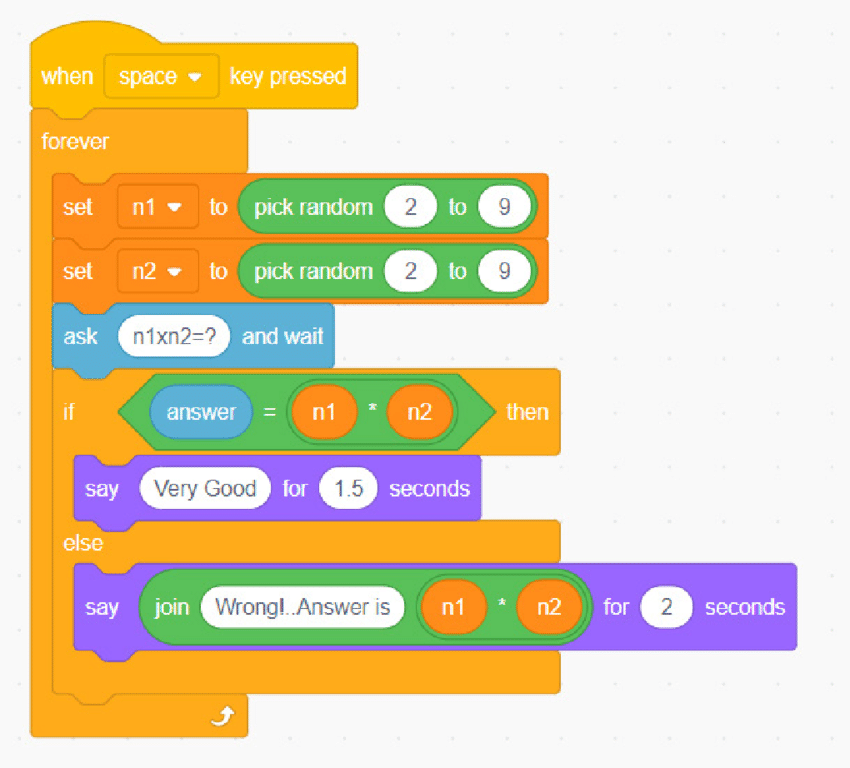
\includegraphics[width=1.0\linewidth]{../../imagens/Scratch-Block.png}
                \caption{Trecho de um c\'odigo em Scratch, em que se v\^e a organiza\c{c}\~ao por blocos, que podem ser montados como num jogo de encaixe. (Fonte: u [[SUNG (2019)]])}
                \label{5cac9c9edeb34a88b5571069bb494cda1ce1bd9c}
\end{minipage}%
\hspace{0.5cm}
\end{figure}



O Scratch re\'une uma comunidade ativa, da qual fazem parte quase 50 milh\~oes de crian\c{c}as, jovens e adultos do mundo inteiro. O Coordenador do Programa WASH teve a oportunidade de conhecer uma das primeiras vers\~oes do Scratch, descrita pessoalmente pelo Prof. Resnick, na \'epoca de seu desenvolvimento.










Ainda h\'a questionamentos sobre a acessibilidade do Scratch, por seu car\'ater visual, cabendo que pesquisadores do mundo todo se debrucem sobre a quest\~ao do design universal, para que pessoas cegas, principalmente, possam usufruir dos mesmos benef\'{\i}cios da ferramenta, que hoje est\~ao restritos aos videntes.










\subsection[O que \'e STEM/STEAM?]{O que \'e STEM/STEAM?}\label{O que \'e STEM/STEAM?}
V\'arios autores  (CATTERALL, 2017)  [XXX Heather Gonzalez e  Tahlea Jankoski, Rodger Bybee] indicam a d\'ecada de 90 do s\'eculo passado como o in\'{\i}cio do uso estruturado do conceito de Science, Technology, Engineering and Mathematics em curr\'{\i}culos escolares, mas o acr\^onimo para represent\'a-lo teve altera\c{c}\~oes ao longo dos anos. Segundo post de Tahlea Jankoski em [XXX https://blog.stemscopes.com/stem-a-rebranded-idea-of-the-past], inicialmente o conceito era representado pela sigla SMET, mas a similaridade de pron\'uncia com a palavra \textquotedbl smut (que significa obscenidade, em ingl\^es) sugeriu a mudan\c{c}a da sigla para METS e depois para STEM, em 2001 [XXX Tahlea Jankoski e Enciclopedia Brittanica].










Autores mencionam a confus\~ao que este termo gera, uma vez que em ingl\^es pode se referir a c\'elulas tronco, com tronco de \'arvore ou com o pedestal de um copo de vinho [XXX Rodger Bybee, ]. Para evitar esse tipo de confus\~ao, \'e poss\'{\i}vel identificar uma recorr\^encia da forma \textquotedbl STEM Education nas publica\c{c}\~oes. Neste trabalho ser\'a usada a forma STEM, em mai\'usculas, para se fazer refer\^encia ao movimento de revis\~ao curricular associado \`as disciplinas de \textquotedbl Science, Technology, Engineering and Mathematics.  










Os Estados Unidos sempre deram import\^ancia para a educa\c{c}\~ao de ci\^encias como pol\'{\i}tica p\'ublica. Uma evid\^encia disso pode ser encontrada nas atas da Conven\c{c}\~ao Constitucional de 1787, a exemplo do que se extrai da \textquotedbl Notes of Debates in the Federal Convention of 1787 [XXX apud Heather Gonzalez]:











\noindent\begin{center}\mbox{\centering\fbox{\centering\par\parbox{0.7\linewidth}{\small\textit{\textquotedbl to establish seminaries for the promotion of literature and the arts and the sciences.}\normalsize}}}\end{center}


Outra evid\^encia pode ser extra\'{\i}da do primeiro discurso do Estado da Uni\~ao do Presidente George Washington [XXX achar data]:











\noindent\begin{center}\mbox{\centering\fbox{\centering\par\parbox{0.7\linewidth}{\small\textit{\textquotedbl Nor am I less persuaded that you will agree with me in opinion that there is nothing which can better deserve your patronage than the promotion of science and literature. Knowledge is in every country the surest basis of public happiness. In one in which the measures of government receive their impressions so immediately from the sense of the community as in ours it is proportionably [sic] essential. 2 (First State of Union Address - President George Washington)}\normalsize}}}\end{center}


Da mesma forma, observadores [XXX Heather Gonzales] tra\c{c}am o lan\c{c}amento do sat\'elite Sputnik, em 1950, como um divisor de \'aguas para o ensino de STEM nos Estados Unidos [XXX Heather Gonzalez].










O movimento pelo STEM, nos Estados Unidos, tem evidente motiva\c{c}\~ao econ\^omica, estrat\'egica e de manuten\c{c}\~ao da hegemonia americana. Uma evid\^encia disso \'e a cita\c{c}\~ao \`a fala do Presidente da Lockheed Martin, Norm Augustine, em outubro de 2012, presente em [XXX James Catterall]:











\noindent\begin{center}\mbox{\centering\fbox{\centering\par\parbox{0.7\linewidth}{\small\textit{\textquotedbl ... industry and government to promote more STEM education in the U.S. ‘Failure to do so... will undermine the U.S. economy, security and place as a world leader.’ Competing with knowledge-based resources will be one way that the U.S. can recover and retain primacy in the global marketplace (Twittweb, 2012).}\normalsize}}}\end{center}


Mas em termos recentes, foi em meados da d\'ecada de 90 que o baixo desempenho comparativo em STEM dos estudantes americanos ganhou notoriedade na imprensa, pela constata\c{c}\~ao de uma sequ\^encia de notas med\'{\i}ocres no Programme for International Student Assessment (PISA)  (CATTERALL, 2017). O PISA \'e um exame internacional promovido pela Organiza\c{c}\~ao para a Coopera\c{c}\~ao e Desenvolvimento Econ\^omico (OCDE), que busca estabelecer um padr\~ao global de avalia\c{c}\~ao, que permita comparar o desempenho de estudantes de diferentes pa\'{\i}ses. Nos dias de hoje, estudantes de cerca de 65 pa\'{\i}ses participam do exame, que \'e considerado um instrumento importante para planejar melhorias nos sistemas educacionais ao redor do mundo.










Em 1998, por meio de um relat\'orio apresentado ao Congresso Americano pelo Committee on Equal Opportunities in Science and Engineering da National Science Foundation, este importante organismo, que seria o equivalente ao nosso CNPq, alerta para a import\^ancia do ensino de STEM nas escolas fundamentais americanas para que os EUA mantenham sua lideran\c{c}a global  (CONGRESS, 1998):











\noindent\begin{center}\mbox{\centering\fbox{\centering\par\parbox{0.7\linewidth}{\small\textit{\textquotedbl In order to maintain its global leadership, America must ensure our citizens can meet the demands of a more scientifically- and technologically-centered world. The National Science Foundation (NSF) has a key role in creating and maintaining the science, mathematics, engineering, and technology (SMET) capacity in this nation. The Committee on Equal Opportunities in Science and Engineering (CEOSE) has been charged by Congress with advising NSF in assuring that all individuals are empowered and enabled to participate fully in the science, mathematics, engineering, and technology (SMET) enterprise.}\normalsize}}}\end{center}


Nesse relat\'orio o NSF usa ainda o acr\^onimo SMET, que em 2001, segundo a enciclop\'edia Brit\^anica teria sido alterado para STEM  (BRITANNICA, 2022a).










As \'areas em que os estudantes americanos n\~ao conseguiam se sobressair, em rela\c{c}\~ao aos demais pa\'{\i}ses desenvolvidos, eram as de ci\^encias, tecnologia e matem\'atica  (CATTERALL, 2017). Essa situa\c{c}\~ao passou a representar inc\^omodo para os gestores educacionais do pa\'{\i}s, dado que n\~ao refletia a sua imagem pr\'opria de pot\^encia internacional  (CATTERALL, 2017), principalmente no campo da ci\^encia e tecnologia. Foi nesse momento que as iniciativas educacionais em \textquotedbl science, technology, engineering and mathematics se destacaram e o acr\^onimo SMET surgiu, posteriormente substitu\'{\i}do por STEM  (CATTERALL, 2017).










Segundo a interpreta\c{c}\~ao da \'epoca, o baixo desempenho americano em STEM tinha rela\c{c}\~ao com a falta de equidade no acesso ao STEM, dentro da realidade das escolas americanas  (CATTERALL, 2017).










Dentre as respostas do governo americano se destacaram o programa \textquotedbl Nenhuma Crian\c{c}a Deixada para Tr\'as, em tradu\c{c}\~ao livre de \textquotedbl No Child Left Behind Act, uma iniciativa de 2002, e o \textquotedbl Todo Estudante ter\'a Sucesso, em tradu\c{c}\~ao livre de \textquotedbl Every Student Succeeds, de 2015  (CATTERALL, 2017).










Mas as respostas americanas n\~ao ficaram restritas \`as esferas de governo, havendo tamb\'em as que foram conduzidas por organiza\c{c}\~oes n\~ao-governamentais, universidades, think-tanks, entre outras.










Em termos epistemol\'ogicos, podemos dizer que o STEAM \'e o sincretismo de diferentes vis\~oes do m\'etodo cient\'{\i}fico, cabendo uma an\'alise individual de cada um, identificado pela primeira letra do acr\^onimo STEAM.










Em  MAMMANA et al. (2020) fizemos uma discuss\~ao sobre a epistemologia subjacente a cada um dos elementos. Sentimo-nos confort\'aveis com a reprodu\c{c}\~ao das ideias aqui, recompiladas, uma vez que somos co-autores do referido relat\'orio. Como exemplos do que descrevemos aqui, nos concentramos na ind\'ustria de semicondutores, \'area de dom\'{\i}nio do co-orientador desta disserta\c{c}\~ao, bem como no campo dos instrumentos de percuss\~ao, \'area na qual esta candidata investiu tempo, atrav\'es de sua participa\c{c}\~ao no grupo cultural \textquotedbl Caixeirosas\textquotedbl . A escolha dos semicondutores (ou chips) como exemplo \'e oportuna, tamb\'em, porque s\~ao esses dispositivos os viabilizadores das tecnologias digitais, fundamentais para a exist\^encia, nos dias de hoje, de uma \textquotedbl cultura digital\textquotedbl . Os chips s\~ao imprescind\'{\i}veis para todos os dispositivos digitais, n\~ao havendo tecnologia substituta.










Um dos pontos altos da discuss\~ao a seguir \'e trazer a interdepend\^encia dos 5 elementos do STEAM.










\'E razo\'avel considerar o m\'etodo de engenharia (E) como sendo derivado do m\'etodo cient\'{\i}fico (S), havendo uma grande interdepend\^encia entre os resultados de um no outro, muito embora seus objetivos sejam diferentes. O desenvolvimento tecnol\'ogico (T) tem na engenharia (E) sua aliada e pode ser considerado, em alguma situa\c{c}\~oes, como decorrente dela, principalmente quando se faz refer\^encia ao termo \textquotedbl alta tecnologia\textquotedbl . Mas n\~ao basta um produto ser baseado em algum conhecimento cient\'{\i}fico para que seja alta tecnologia. De forma gen\'erica, \'e poss\'{\i}vel dizer que \textquotedbl alta tecnologia\textquotedbl  \'e uma alus\~ao a processos de manufatura complexos, com muitas etapas de alto grau de risco de sucesso cada uma, o qual pode ser mitigado atrav\'es do emprego de alguma forma de conhecimento cient\'{\i}fico.










Um exemplo de alta tecnologia \'e a manufatura de circuitos integrados, ou chips. Os chips s\~ao circuitos eletr\^onicos ultra-miniaturizados cuja produ\c{c}\~ao requer entre dezenas e centenas de etapas de processo. A exist\^encia de uma \textquotedbl Cultura Digital\textquotedbl  \'e diretamente relacionada ao sucesso da ind\'ustria de Chips, que, al\'em de desenvolver os dispositivos em si, que sustentam as redes digitais contempor\^aneas, conseguiu desenvolver os conhecimentos necess\'arios para contornar o alto risco de suas etapas de produ\c{c}\~ao, conduzindo para um processo que hoje tem alta produtividade. Nesse exemplo dos chips, a engenharia teve papel preponderante e muitos outros exemplos da contribui\c{c}\~ao da engenharia para a tecnologia podem ser citados.










Por sua rela\c{c}\~ao com a engenharia, \'e natural considerar que a tecnologia tamb\'em pode estar relacionada ao m\'etodo cient\'{\i}fico, muito embora n\~ao devesse ser condundida com a ci\^encia em si. As pessoas tendem a confundir os conceitos de tecnologia e ci\^encia, assumindo que a primeira (T) \'e decorrente da segunda (C). Entretanto, defendemos que n\~ao existe depend\^encia intr\'{\i}nseca entre tecnologia e ci\^encia. Os processos que levam ao estabelecimento de (T) podem ter contextos cognitivos, sensoriais e culturais n\~ao formais, independentes de (C). Ent\~ao vale a pena refletir sobre situa\c{c}\~oes em que a tecnologia pode se desenvolver por outros meios, que n\~ao os cient\'{\i}ficos.










Continuamente aproveitando os resultados de nossa reflex\~ao registrada em  MAMMANA et al. (2020), vamos nos debru\c{c}ar de forma um pouco mais estendida sobre essa quest\~ao, criando uma hip\'otese sobre o desenvolvimento de instrumentos musicais.










O ser humano tem a necessidade constante de expressar seus sentimentos e emo\c{c}\~oes, e faz isso atrav\'es do est\'{\i}mulo \`as percep\c{c}\~oes e sensa\c{c}\~oes em si e nos outros. Reduzida a um contexto instrumental, a arte (A) pode ser considerada como uma concretiza\c{c}\~ao da comunica\c{c}\~ao destas percep\c{c}\~oes e sensa\c{c}\~oes entre os indiv\'{\i}duos, tendo um car\'ater muito mais amplo do que a pr\'opria ci\^encia, a tecnologia ou a engenharia. Por outro lado, o est\'{\i}mulo m\'utuo sempre requer alguma forma de intera\c{c}\~ao por meio dos sentidos, a qual, por sua vez, exige o emprego de meios materiais, diretos ou indiretos. Por exemplo, a arte pode depender de instrumentos musicais, de tintas coloridas ou de ferramentas de corte para esculpir, por exemplo. Todos estes meios t\^em um certo grau de depend\^encia dos conhecimentos da ci\^encia, da engenharia e da tecnologia.










Em oposi\c{c}\~ao, podemos imaginar situa\c{c}\~oes em que as artes pl\'asticas s\~ao desempenhadas por artes\~aos, ou outros profissionais artistas sem reconhecimento acad\^emico formal, mas que dominam gestos e t\'ecnicas complexos. Quando o homem esticou a primeira pele de animal para produzir um tambor primitivo, talvez (apenas por hip\'otese) tenha sido motivado pela necessidade org\^anica de reproduzir sons peri\'odicos, tais como seus pr\'oprios batimentos card\'{\i}acos. Eles sutilmente acompanham os seres humanos por toda a vida e t\^em um papel na no\c{c}\~ao de ritmo. \'E imposs\'{\i}vel ter certeza, mas podemos imaginar, como apoio ret\'orico, de que forma o conhecimento necess\'ario para esticar a pele do tambor surgiu. \'E plaus\'{\i}vel que os processos que levaram ao gesto de esticar a pele para gerar o tambor, bem como o gesto de \textquotedbl bater\textquotedbl  na pele com as m\~aos, podem n\~ao ter se originado num modelo formal, mas simplesmente num acidente sensorial-cognitivo. Este \'e um poss\'{\i}vel exemplo no qual a tecnologia (de fazer um tambor) se desenvolve independentemente de um conhecimento formal, o qual, por seu lado seria t\'{\i}pico da esfera da ci\^encia e da engenharia.










Do ponto de vista da motiva\c{c}\~ao para a produ\c{c}\~ao do som, pertinente \`a esfera da arte (A), o que se deu foi a necessidade de fazer o outro receber est\'{\i}mulos diversos. A partir deles, o receptor teve a oportunidade de alterar seu estado cognitivo e sensorial, com a produ\c{c}\~ao de emo\c{c}\~oes que s\~ao re-interpreta\c{c}\~oes das que motivaram a express\~ao percursiva original.










A percuss\~ao, talvez a primeira forma de m\'usica, tem base fisiol\'ogica e se estabelece a partir de seu elemento percursor: o ritmo. Entretanto, n\~ao necessariamente tem origem num formaliza\c{c}\~ao de algum conhecimento. N\~ao obstante essa independ\^encia, tamb\'em incentiva o desenvolvimento de instrumentos, o que, ironicamente, pode requerera formaliza\c{c}\~ao de conhecimentos, dependendo da complexidade do instrumento.










Independentemente de como foi a g\^enese dos conhecimentos que levaram \`a produ\c{c}\~ao do tambor, h\'a muito tempo existem t\'ecnicas espec\'{\i}ficas para esticar a pele do tambor, para achar o local dos furos da flauta ou para construir um violino. Muitas s\~ao totalmente sensoriais, envolvendo tamb\'em o dom\'{\i}nio de gestos (e.g. entalhe do pesco\c{c}o do viol\~ao), outras s\~ao formais, requerendo muitas etapas de processamento f\'{\i}sico-qu\'{\i}mico (e.g. recobrimento met\'alico do saxofone). Isso, por si s\'o, mostra que a arte, em sua busca pela express\~ao de sentimentos e emo\c{c}\~oes, tamb\'em \'e um motor da tecnologia. O mesmo racioc\'{\i}nio \'e v\'alido para as artes pl\'asticas, a arquitetura, a produ\c{c}\~ao \'audio-visual, etc. Todas estimularam a cria\c{c}\~ao e se beneficiaram de novas tecnologias.










A matem\'atica (M) \'e o quinto elemento presente no STEAM. O debate sobre se a matem\'atica teria sido descoberta ou inventada \'e intermin\'avel. Conquanto esta incerteza, o fato \'e que em muitos momentos as teorias matem\'aticas abstratas precederam a percep\c{c}\~ao e entendimento dos fen\^omenos naturais, \`as quais foi preciso recorrer para sua compreens\~ao. Nas viv\^encias envolvendo STEAM, a matem\'atica \'e um dos elementos centrais, que alimenta todos os demais, seja no momento de modelar geometricamente o comportamento de um dispositivo de caracteriza\c{c}\~ao meteorol\'ogica (e.g. pluvi\^ometro de b\'ascula baseado em sucata), seja na hora de construir um algoritmo de programa de computador (e.g. plano cartesiano).










Como dissemos, as reflex\~oes que expusemos aqui buscam justamente mostrar a inter-depend\^encia dos cinco conceitos que formam o STEAM, sem a preval\^encia de um sobre o outro, num fluxo harm\^onico e complementar de troca de informa\c{c}\~oes, motiva\c{c}\~oes e resultados.











\noindent\begin{center}\mbox{\centering\fbox{\centering\par\parbox{0.7\linewidth}{\small\textit{\'E essa mistura dos cinco elementos que traz a for\c{c}a do STEAM como instrumento de aprendizagem. Nada mais oportuno do que deixar que as crian\c{c}as fa\c{c}am suas \textquotedbl pescarias\textquotedbl , usufruindo do imbricamento que estes 5 mundos conectados t\^em. Do ponto de vista do educando, o conjunto representado pelo STEAM oferece um universo ilimitado de aprendizados, todos muito relevantes para seu futuro, seja professional, social ou pessoal. Dominar conhecimentos pertinentes ao STEAM \'e cada vez mais determinante para a capacidade do ser humano de se inserir em sua pr\'opria cultura de forma aut\^onoma. (Fonte:  MAMMANA et al. (2020))}\normalsize}}}\end{center}


Acreditamos que as novas diretrizes para o ensino m\'edio, com o estabelecimento da Base Nacional Comum Curricular (BNCC) permitam aprofundar o emprego da abordagem STEAM na escola p\'ublica brasileira, como mais um elemento a contribuir com a redu\c{c}\~ao da evas\~ao escolar e das vulnerabilidades sociais  (MAMMANA et al., 2020b).










\section[Fundamenta\c{c}\~ao: modelagem (eixo 2)]{Fundamenta\c{c}\~ao: modelagem (eixo 2)}\label{Fundamenta\c{c}\~ao: modelagem (eixo 2)}
Vimos que o objeto desta pesquisa \'e caracteriza\c{c}\~ao do Programa WASH, no recorte de novembro de 2013 at\'e outubro de 2022, abordando 3 eixos que se complementam.










Como o objetivo deste trabalho \'e propor uma melhoria no Programa WASH, atrav\'es da revis\~ao de seu termo de refer\^encia, e, considerando que o WASH tamb\'em pode ser considerado como uma organiza\c{c}\~ao (como j\'a visto), n\~ao seria surpresa se algu\'em propusesse o emprego de m\'etodos de administra\c{c}\~ao pertinentes \`a disciplina de \textquotedbl Organiza\c{c}\~ao, Sistemas de M\'etodos\textquotedbl  (OSM), por exemplo.











\noindent\begin{center}\mbox{\centering\fbox{\centering\par\parbox{0.7\linewidth}{\small\textit{Organiza\c{c}\~ao, Sistemas e M\'etodos \'e uma \'area da administra\c{c}\~ao que lida com um conjunto de t\'ecnicas que t\^em como objetivo principal aperfei\c{c}oar o funcionamento das organiza\c{c}\~oes. (Fonte:  CARDOSO (2014) )}\normalsize}}}\end{center}


No entanto, o WASH n\~ao pode ser considerada uma institui\c{c}\~ao  dentro do Servi\c{c}o P\'ublico Federal e, por isso, carece de equipe est\'avel, documento formal de institucionaliza\c{c}\~ao. O WASH n\~ao tem organograma e, portanto, näo est\'a formalizada uma hierarquia, t\~ao cara \`as corpora\c{c}\~oes. Dentro da classifica\c{c}\~ao de organiza\c{c}\~oes oferecida por  MAXIMIANO (1981), o WASH n\~ao se encaixa integralmente em \textquotedbl Grupos Sociais Secund\'arios\textquotedbl , que \'e justamente o grupo que tem caracter\'{\i}sticas de institucionaliza\c{c}\~ao adequadas para o emprego da OSM.










Por esse motivo, decidimos concentrar nossos esfor\c{c}os  em m\'etodos de modelagem n\~ao restritos ao universo de corpora\c{c}òes, que permitam complementar o m\'etodo historiogr\'afico, sem excluir integralmente a possibilidade de emprego de t\'ecnicas praticadas no contexto do OSM, a exemplo do Business Process Modeling Notation (BPMN).










No campo da engenharia existe toda uma \'area conhecida como Unified Modeling Language (UML), que permite trabalhar com requisitos do sistema, casos de uso, descri\c{c}\~ao de atividades, entre outros meios descritivos. Mas n\~ao seguiremos esse caminho, como se ver\'a nos Materiais e M\'etodos, permanecendo na zona proximal de nossa forma\c{c}\~ao acad\^emica, que \'e na \'area de humanas. Mostraremos que nossa abordagem \'e capaz de gerar uma modelagem pass\'{\i}vel de ser complementada pela \'area de Engenharia posteriormente.










A nossa modelagem, principalmente a de dados, busca enfrentar o desafio do \textquotedbl aumento das fontes imag\'eticas, dos recursos relativos \`a inform\'atica e a infla\c{c}\~ao arquiv\'{\i}stica que produz um excesso de documentos\textquotedbl   (DOSSE, 2012) para serem tratados pela historiografia.










Sem um aprisionamento aos conceitos do mundo corporativo ou da engenharia, usaremos formas de modelar o sistema WASH que permitam trazer informa\c{c}\~oes sobre seus m\'etodos e resultados, complementando o trabalho historiogr\'afico, como segue:











\begin{alineas}
\item na descri\c{c}\~ao de suas entidades e relacionamentos (Setzer e Silva, 2017)
\item na descri\c{c}\~ao de seus processos (e.g. por meio de um diagrama tipo Business Process Modeling and Notation - BPMN)
\end{alineas}

A profundidade da modelagem depende do n\'{\i}vel de abstra\c{c}\~ao a que se quer chegar na an\'alise do sistema do WASH.










Setzer e Silva (2017) ensinam que h\'a 4 n\'{\i}veis de abstra\c{c}\~ao para analisar um sistema do mundo real:














\begin{table}[htb]
\tiny
\caption{\label{98b39a827ce08562e7aeba26851f8d86d1af7179}N\'{i}veis de abstra\c{c}\~oes}

\centering
\begin{tabular}{|c|c|}
\hline
Modelo Descritivo  &  modelo do n\'{\i}vel de abstra\c{c}\~ao descritivo \\
\hline
Modelo Conceitual  &  modelo do n\'{\i}vel de abstra\c{c}\~ao conceitual \\
\hline
Modelo Computacional  &  linguagens de computa\c{c}\~ao de alto n\'{\i}vel \\
\hline
Modelo Interno  &  linguagem de programa\c{c}\~ao \\
\hline
\end{tabular}
\end{table}


Considerando os objetivos da caracteriza\c{c}\~ao aqui almejados, neste trabalho a an\'alise do Sistema do WASH ficar\'a concentrada no modelo do n\'{\i}vel de abstra\c{c}\~ao descritivo (ou simplesmente Modelo Descritivo), que se diferencia por usar uma linguagem informal. Este n\'{\i}vel de abstra\c{c}\~ao ser\'a usado para a identifica\c{c}\~ao das entidades envolvidas, bem como suas associa\c{c}\~oes  (Setzer e Silva, 2017). A abordagem do Modelo Descritivo ser\'a complementada com \textquotedbl pinceladas\textquotedbl  do modelo do n\'{\i}vel de abstra\c{c}\~ao conceitual (ou simplesmente Modelo Conceitual), que ser\'a usado para a representa\c{c}\~ao dos relacionamentos entre entidades.










A figura XXX mostra um diagrama da abordagem adotada neste trabalho, que pode ser identificada como \textquotedbl Modelo H\'{\i}brido\textquotedbl , por combinar os n\'{\i}veis de abstra\c{c}\~ao descritivo e conceitual.










Na figura vemos v\'arios acr\^onimos que ser\~ao muito importantes para n\'os daqui para frente e dedicaremos alguns par\'agrafos para descrev\^e-los.










O primeiro acr\^onimo de grande import\^ancia \'e MER, que significa Modelo Entidade Relacionamento. Este tipo de modelo \'e descrito em detalhes por Setzer e Silva (2017), e busca identificar as entidades que precisam ser representadas pelos dados, bem como suas associa\c{c}\~oes (ou relacionamentos). O MER pode ser constru\'{\i}do tanto no n\'{\i}vel descritivo quanto no n\'{\i}vel conceitual. Um outro acr\^onimo que aparece na figura derivado do MER \'e o ER, que significa simplesmente \textquotedbl Entidade Relacionamento\textquotedbl . Na figura o acr\^onimo ER est\'a sendo usado para designar o tipo de diagrama que \'e empregado no n\'{\i}vel conceitual.










O acr\^onimo MDR se refere a Modelo de Dados Relacionais, que \'e uma abstra\c{c}\~ao mais profunda do Modelo Entidade Relacionamento. O MDR j\'a traz elementos de implementa\c{c}\~ao dos dados no sistema computacional e pode ser descrito na linguagem Structured Query Language, cujo acr\^onimo \'e SQL.










O acr\^onimo PHP indica uma linguagem de programa\c{c}\~ao usada no servidor web. Este acr\^onimo, do tipo recursivo, representa Hypertext Preprocessor. O termo Javascript \'e uma linguagem que, diferentemente do PHP, \'e usada no cliente.












\captionsetup{format=plain}
\begin{figure}[htb]

	\begin{center}

		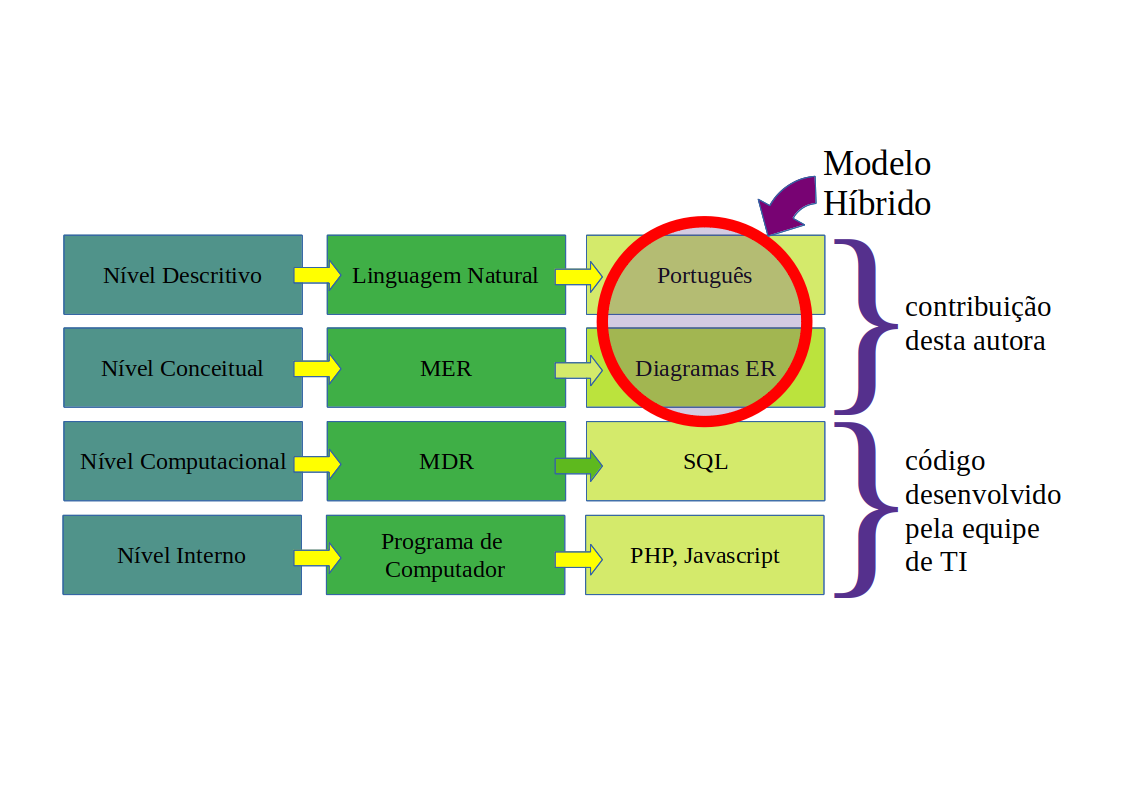
\includegraphics[max size={\textwidth}{\textheight}]{../../imagens/niveis-abstracao.png}

	\end{center}

	\caption{\label{057551752fd94508086a839f982c9c3e7ef2688d}Diagrama que mostra os quatro n\'{i}veis de abstra\c{c}\~ao para a an\'alise de um sistema. Neste trabalho ser\'a usado um m\'etodo h\'{i}brido.}

\end{figure}

Al\'em da modelagem indicada, pertinente \`a identifica\c{c}\~ao de entidades e relacionamento, nos dedicaremos \`a modelagem de processos, atrav\'es do desenvolvimento de um diagrama BPMN. Este diagrama foi desenvolvido pelo colega Saulo Monteiro, a pedido da coordena\c{c}\~ao do WASH. O modelo BPMN em quest\~ao foi baseado em informa\c{c}\~oes sobre os procedimentos de implanta\c{c}\~ao do WASH desenvolvidos pela candidata, raz\~ao pela qual sua apresenta\c{c}\~ao neste disserta\c{c}\~ao \'e adequada.










Mas antes de partir para a descri\c{c}\~ao da modelagem de sistemas, faremos uma breve revis\~ao do conceito de Taxonomia, dado que ser\'a importante para associa\c{c}\~oes de classifica\c{c}\~ao do Modelo MER.










\subsection[Taxonomia]{Taxonomia}\label{Taxonomia}
A taxonomia originou-se no contexto da biologia, como forma de classifica\c{c}\~ao cient\'{\i}fica dos seres vivos, \'area cujo pioneiro foi Carolus Linnaeus, bot\^anico, zo\'ologo e m\'edico Sueco nascido em 1707.










Sin\^onimo de \textquotedbl classifica\c{c}\~ao\textquotedbl   (MARTINEZ et al., 2004), passou a ser usada como forma de organiza\c{c}\~ao do conhecimento em muitos outros campos.










Para come\c{c}ar a conceitu\'a-la, vamos adotar uma vis\~ao simplificada da taxonomia, em que apenas um n\'{\i}vel hier\'arquico \'e considerado, para depois ampliar nosso entendimento para mais n\'{\i}veis.










No contexto no qual aqui temos que trabalhar, podemos considerar a Taxonomia como uma aplica\c{c}\~ao da teoria de conjuntos origin\'aria da matem\'atica. Por meio dela buscam-se formas de organizar o conhecimento em \textquotedbl conjuntos disjuntos dois a dois\textquotedbl , ou seja, conjuntos que n\~ao t\^em elementos em comum.










Considere os conjuntos de letras da tabela XXX.














\begin{table}[htb]
\tiny
\caption{\label{44490fe2b906078abd65fafd043ad29728406f42}Exemplo de 3 conjuntos disjuntos dois a dois.}

\centering
\begin{tabular}{|c|c|}
\hline
Nome do Conjunto  &  Conte\'udo do Conjunto \\
\hline
Conjunto 1  &  A, H, M, N, S \\
Conjunto 2  &  B, O \\
Conjunto 3  &  C, Y, J \\
\hline
\end{tabular}
\end{table}


Os conjuntos 1, 2 e 3 definidos acima s\~ao \textquotedbl disjuntos dois-a-dois\textquotedbl , porque n\~ao t\^em elementos repetidos.










Agora vamos analisar uma situ\c{c}\~ao em que os conjuntos n\~ao s\~ao disjuntos dois a dois. Considere a tabela XXX.














\begin{table}[htb]
\tiny
\caption{\label{9ff362cd60f20203c10ee684d58cf4dec084efbb}Exemplo de 3 conjuntos que n\~ao s\~ao disjuntos dois a dois.}

\centering
\begin{tabular}{|c|c|}
\hline
Nome do Conjunto  &  Conte\'udo do Conjunto \\
Conjunto 4  &  A, H, M, N, S \\
Conjunto 5  &  B, T, O, M \\
Conjunto 6  &  C, Y, J \\
\hline
\end{tabular}
\end{table}


Os tr\^es conjuntos acima n\~ao s\~ao disjuntos dois a dois, porque o Conjunto 4 e o Conjunto 5 cont\'em a letra M e, portanto, a intersec\c{c}\~ao dos dois n\~ao \'e nula. Evidente que os Conjuntos 4 e 6, quando considerados sem o Conjunto 5, s\~ao \textquotedbl disjuntos dois a dois\textquotedbl , mas essa afirma\c{c}\~ao deixa de ser v\'alida quando o Conjunto 5 passa a ser considerado tamb\'em.










Agora que sabemos que uma taxonomia \'e uma forma de organizar o conhecimento em conjuntos disjuntos dois a dois, vamos ver na pr\'atica como isso funciona.










Imaginemos um jeito de organizar ve\'{\i}culos automotores em conjuntos. Vamos dividir os ve\'{\i}culos entre \textquotedbl carros\textquotedbl  e \textquotedbl motocicletas\textquotedbl . Essa \'e um taxonomia funcional, porque carros t\^em exatamente 4 rodas e motos t\^em exatamente 2 rodas, portanto \'e imposs\'{\i}vel que um elemento do conjunto carros apare\c{c}a no conjunto motos, porque um dado ve\'{\i}culo n\~ao tem como ter exatamente 4 rodas e exatamente 2 rodas ao mesmo tempo. O termo \textquotedbl exatamente\textquotedbl  est\'a sendo usado aqui no sentido de \textquotedbl nem mais nem menos do que um determinado valor\textquotedbl . \'E muito importante usar o termo \textquotedbl exatamente\textquotedbl  neste caso porque, de outra forma, carros poderiam estar tamb\'em no conjunto de motos, porque carros t\^em 4 rodas, mas tamb\'em t\^em duas. Claro que para alguns isso pode parecer um preciosismo, mas \'e sempre importante tentar buscar o uso preciso da linguagem.










Agora vamos pensar em uma outra forma de agrupar ve\'{\i}culos automotores: conjuntos de \textquotedbl carros\textquotedbl , conjunto de \textquotedbl motocicletas\textquotedbl  e conjuntos de \textquotedbl ve\'{\i}culos azuis\textquotedbl . Essa n\~ao \'e uma taxonomia funcional, porque permite ter a repeti\c{c}\~ao do elemento \textquotedbl carro azul\textquotedbl  tanto no grupo \textquotedbl carros\textquotedbl  (porque \textquotedbl carro azul\textquotedbl  tem exatamente 4 rodas) quanto no grupo \textquotedbl ve\'{\i}culos azuis\textquotedbl  (porque \textquotedbl carro azul\textquotedbl  \'e um \textquotedbl ve\'{\i}culo azul\textquotedbl ). Assim, a informa\c{c}\~ao dividida nos tr\^es grupos indicados n\~ao forma conjuntos disjuntos dois a dois, dado que pelo menos 1 elemento aparece em dois conjuntos diferentes.










Uma outra forma de pensarmos essa \textquotedbl taxonomia de conjuntos disjuntos\textquotedbl  \'e considerar a \'arvore de diret\'orios de um sistema operacional, como Linux ou Windows, na sua forma mais b\'asica (sem links l\'ogicos).










Numa \'arvore de diret\'orios b\'asica, cada arquivo s\'o consegue estar em um diret\'orio de cada vez (desconsidere c\'opias de arquivos).










Assim, pelo que descrevemos at\'e agora, a taxonomia \'e uma forma de organizar a informa\c{c}\~ao hierarquicamente, classificando-a em categorias ou tipos. Mas como funciona essa hierarquia?










Segundo  VITAL e CAF\'E (2011), \textquotedbl a taxonomia organiza a informa\c{c}\~ao da mais gen\'erica a mais espec\'{\i}fica, utilizando uma rela\c{c}\~ao hier\'arquica ou rela\c{c}\~ao de g\^enero-esp\'ecie entre os termos\textquotedbl .










 VITAL e CAF\'E (2011), citando Dalberg, definem essa rela\c{c}\~ao hier\'arquica como a que aparece \textquotedbl (...) entre dois conceitos que t\^em id\^enticas caracter\'{\i}sticas, sendo por\'em, que uma em rela\c{c}\~ao \`a outra, apresenta uma caracter\'{\i}stica adicional, de modo que surge entre eles uma hierarquia\textquotedbl .










Como exemplo dessa forma hierarquizada de representa\c{c}\~ao, podemos pensar na classifica\c{c}\~ao dos documentos do Programa WASH por tipos de documentos, como indicado na Fig. XXX.












\captionsetup{format=plain}
\begin{figure}[htb]

	\begin{center}

		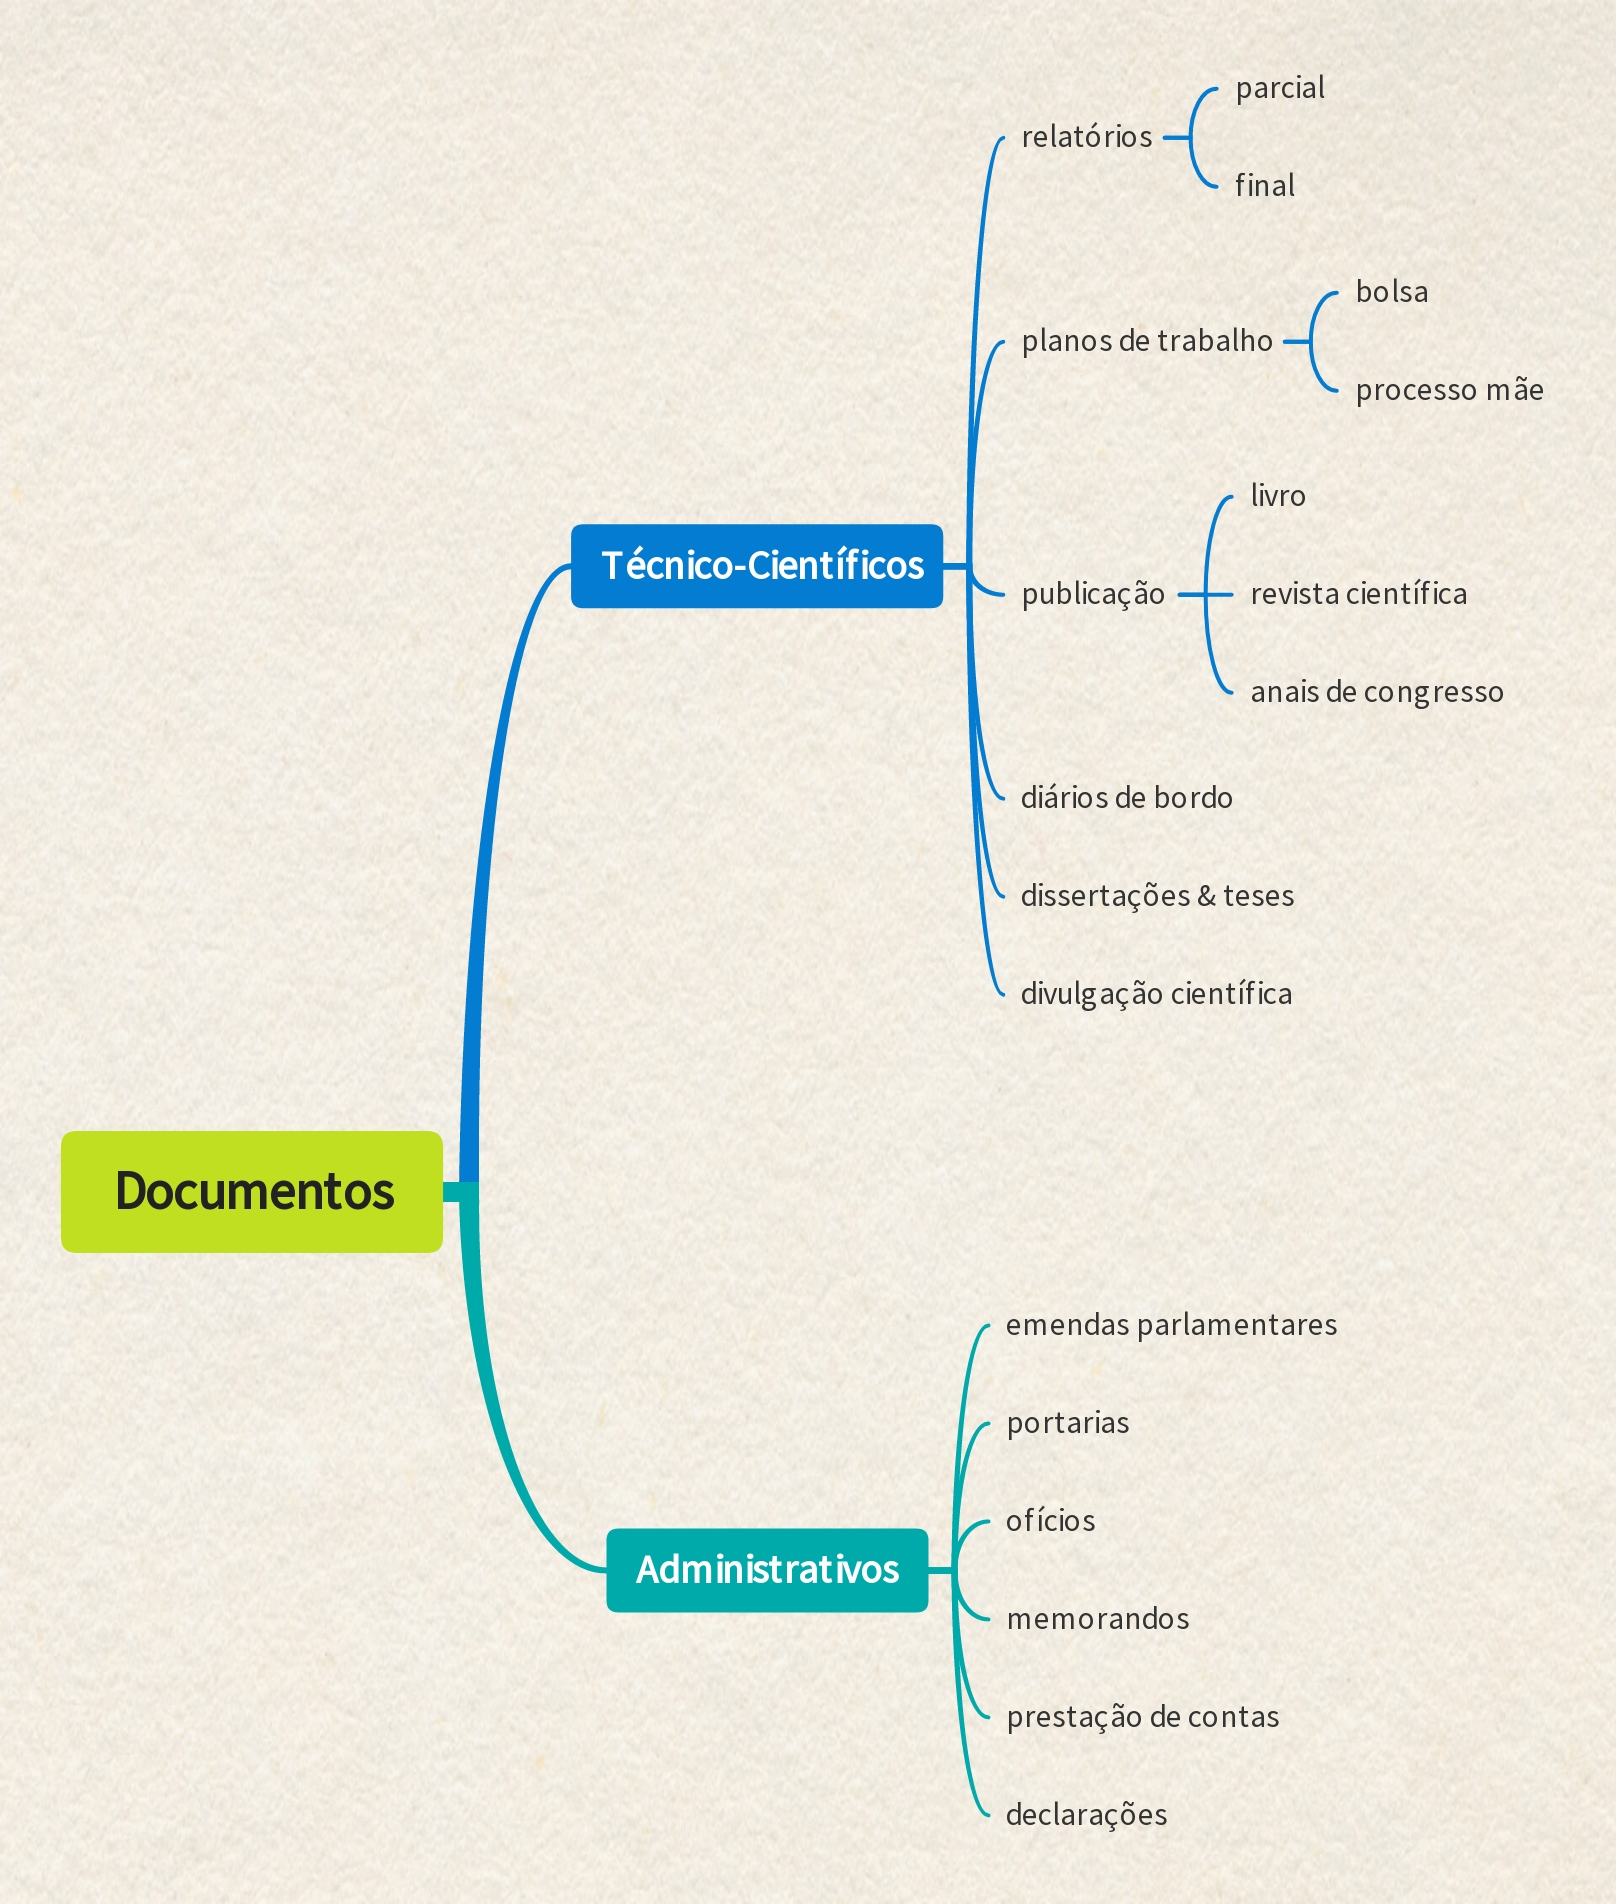
\includegraphics[max size={\textwidth}{\textheight}]{../../imagens/exemplo-de-taxonomia.jpg}

	\end{center}

	\caption{\label{1d3efc4f11ba26e8cf5155309b9993914a803998}Exemplo de taxonomia de documentos.}

\end{figure}

Vemos que quando o documento est\'a classificado na caixinha de \textquotedbl relat\'orios parciais\textquotedbl , n\~ao tem como ser classificado na caixinha de \textquotedbl relat\'orios finais\textquotedbl , porque um relat\'orio n\~ao pode ser classificado como parcial e final ao mesmo tempo: ou ele \'e um relat\'orio parcial, ou \'e um relat\'orio final.










A mesma situa\c{c}\~ao ocorre quando um documento \'e classificado como \textquotedbl plano de trabalho de processo m\~ae\textquotedbl : \'e imposs\'{\i}vel esse documento ser classificado, ao mesmo tempo, como \textquotedbl plano de trabalho de bolsa\textquotedbl , simplesmente porque s\~ao tipos de documentos diferentes.










Por outro lado, um documento do tipo \textquotedbl relat\'orio parcial\textquotedbl  tamb\'em \'e um documento do tipo \textquotedbl relat\'orio\textquotedbl , mas com uma caracter\'{\i}stica adicional: sua parcialidade no tempo. O \textquotedbl relat\'orio\textquotedbl  por sua vez, tamb\'em \'e um documento do tipo \textquotedbl T\'ecnico-Cient\'{\i}fico\textquotedbl , mas com uma caracter\'{\i}stica adicional: o fato de ser um relato sobre resultados obtidos na execu\c{c}\~ao de um plano de trabalho, por exemplo. \'E a essas \textquotedbl caracter\'{\i}sticas adicionais\textquotedbl  que se referia Dahlberg  (apud, VITAL e CAF\'E, 2011).










Um dos grandes desafios do Programa WASH \'e encontrar classifica\c{c}\~oes hier\'arquicas para:











\begin{alineas}
\item \textquotedbl tipos de documentos\textquotedbl ,
\item \textquotedbl \'areas de conhecimento dos projetos de inicia\c{c}\~ao cient\'{\i}fica\textquotedbl ,
\item \textquotedbl temas de oficinas\textquotedbl 
\item \textquotedbl tipos de institui\c{c}\~oes\textquotedbl ,
\item e \textquotedbl atividades de eventos\textquotedbl 
\end{alineas}

que produzam conjuntos disjuntos dois a dois, ou seja, taxonomias vi\'aveis.










Em alguns casos, por simplifica\c{c}\~ao, renunciamos, por enquanto, da busca por hierarquiza\c{c}\~ao no caso de \textquotedbl temas de oficinas\textquotedbl  e \textquotedbl tipos de atividades\textquotedbl , mantendo essa ambi\c{c}\~ao para \textquotedbl tipos de documentos\textquotedbl , \textquotedbl \'areas de conhecimento\textquotedbl  e \textquotedbl tipos de institui\c{c}\~oes\textquotedbl .










Antes de encerrar esse tema, \'e importante registrar as limita\c{c}\~oes da aplica\c{c}\~ao de taxonomias no campo das organiza\c{c}\~oes, como bem apontado por Woods  (apud, VITAL e CAF\'E, 2011): \textquotedbl uma taxonomia cl\'assica sup\~oe que cada elemento s\'o pode pertencer a um ramo da \'arvore hier\'arquica. No entanto, em um ambiente corporativo isso n\~ao \'e poss\'{\i}vel nem desej\'avel\textquotedbl .










\subsection[Modelo Descritivo]{Modelo Descritivo}\label{Modelo Descritivo}
Segundo Setzer e Silva (2017), o modelo descritivo \'e baseado em \textquotedbl descri\c{c}\~oes informais feitas em uma linguagem natural\textquotedbl  tanto escrita quanto falada, ou seja, no presente caso, o modelo descritivo pode ser feito em Portugu\^es.










O n\'{\i}vel do Modelo Descritivo n\~ao requer descri\c{c}\~oes formais:











\noindent\begin{center}\mbox{\centering\fbox{\centering\par\parbox{0.7\linewidth}{\small\textit{(no n\'{\i}vel descritivo) as abstra\c{c}\~oes podem abranger uma gama muito ampla, desde asser\c{c}\~oes logicamente perfeitas at\'e frases amb\'{\i}guas ou mesmo po\'eticas, contendo um simbolismo que transcende a experi\^encia sensorial direta. O importante \'e que haja uma descri\c{c}\~ao por meio de frases (ou outros meios como figuras e fotos), preferivelmente sem o uso de conceitos matematicamente formais, ou pelo menos com um m\'{\i}nimo deles (Setzer e Silva, 2017)}\normalsize}}}\end{center}


O n\'{\i}vel conceitual est\'a \textquotedbl um degrau mais profundo\textquotedbl  na modelagem do sistema, em que \textquotedbl o modelo desenvolvido deve ser estritamente formal\textquotedbl  (Setzer e Silva, 2017).










Considerando esta classifica\c{c}\~ao de n\'{\i}veis de abstra\c{c}\~ao de Setzer e buscando um grau de objetividade adequado, decidimos construir uma modelagem intermedi\'aria entre os n\'{\i}veis descritivo e conceitual, com base no M\'etodo de Entidade e Relacionamento (MER), criando uma forma h\'{\i}brida. Para isso, substitu\'{\i}mos o conceito de \textquotedbl relacionamento\textquotedbl  entre entes pelo de \textquotedbl associa\c{c}\~ao\textquotedbl , uma dica trazida por  Setzer e Silva (2017) na p\'ag. 33 de seu livro.










Assim, no n\'{\i}vel conceitual, os diagramas formais de Entidade Relacionamento ser\~ao usados numa forma simplificada, sendo complementados, no n\'{\i}vel descritivo, por frases que explicam o papel das entidades e de suas associa\c{c}\~oes.










Destarte, para que essa forma de modelar possa ser conduzida com um m\'{\i}nimo de objetividade, ser\'a preciso rever os conceitos b\'asicos do MER.










\subsection[Modelo Entidade Relacionamento (MER)]{Modelo Entidade Relacionamento (MER)}\label{Modelo Entidade Relacionamento (MER)}
A Modelagem tipo Entidade Relacionamento (MER) foi introduzida por Peter Chen em 1976. Setzer e Silva (2017) alertam para a confus\~ao que normalmente \'e feita entre o conceito de Entidade e as tabelas dos Modelos de Dados Relacionais (MDR), os quais ser\~ao mais aprofundados em pr\'oximas se\c{c}\~oes.










A principal diferen\c{c}a entre a MER e os MDR \'e que a primeira \'e totalmente conceitual, n\~ao havendo, necessariamente, identidade direta com a implementa\c{c}\~ao do MDR feita em um computador  (Setzer e Silva, 2017).










Entretanto, as duas representa\c{c}\~oes t\^em paralelos, dado que em muitos casos \'e poss\'{\i}vel correlacionar uma entidade do Modelo MER com uma tabela no MDR. Dito isso, permanece o alerta de  Setzer e Silva (2017) para que n\~ao se confundam entidades com tabelas.










Portanto, o MDR \'e um modelo computacional que visa a sua implementa\c{c}\~ao em um programa de computador, ao passo que o MER visa promover a compreens\~ao do sistema em an\'alise, sem o compromisso de que haver\'a uma implementa\c{c}\~ao em um equipamento inform\'atico.










\'E boa pr\'atica que o MER seja constru\'{\i}do antes do MDR, mas para acelerar resultados, muitos desenvolvedores acabam desenvolvendo o MDR sem uma modelagem MER. Este \'e o caso da plataforma Platu\'osh, cujo MDR foi implementado sem a exist\^encia de um MER. Uma de nossas contribui\c{c}\~oes neste trabalho \'e criar o primeiro MER para o WASH, que permitir\'a avaliar o MDR implementado na forma da Platu\'osh, identificando suas fragilidades e propondo melhorias.










Pode-se dizer que o principal trabalho na modelagem MER \'e identificar as entidades presentes no sistema em an\'alise, no caso o Sistema WASH. Em seguida, um trabalho importante \'e identificar seus relacionamentos.










Entidades s\~ao abstra\c{c}\~oes mentais de um ente que existe no mundo real  (Setzer e Silva, 2017).










Ent\~ao, podem ser consideradas como entidades as representa\c{c}\~oes abstratas de um ser, de uma coisa, de um organismo social, de um sentimento, etc.










Aprofundando um pouco na oferta de exemplos, podem ser modeladas como entidades: uma empresa, seus funcion\'arios, os seus ve\'{\i}culos, os livros da sua biblioteca, seus contratos com clientes ou com trabalhadores, seus processos de neg\'ocios, suas contas banc\'arias, entre tantas outras formas de exist\^encia conceitual.










O sistema de modelagem MER \'e muito formal e define at\'e como as entidades devem ser representadas em diagramas. Por exemplo, uma entidade, na modelagem MER, precisa ter um nome no plural, com a primeira letra mai\'uscula e precisa ser representada num ret\^angulo.










Mas estas regras de representa\c{c}\~ao s\~ao v\'alidas no n\'{\i}vel de abstra\c{c}\~ao conceitual e, como j\'a dissemos, neste trabalho permaneceremos no n\'{\i}vel de abstra\c{c}\~ao descritivo com \textquotedbl leves pinceladas\textquotedbl  do n\'{\i}vel conceitual, removendo a necessidade de formaliza\c{c}\~ao e permitindo que seja baseado em linguagem natural (portugu\^es).










No MER as entidades podem ser consideradas como conjuntos de entes. Assim \'e poss\'{\i}vel pensar na entidade entitulada \textquotedbl Pessoas\textquotedbl  como um conjunto de pessoas, por exemplo.










Sem a pretens\~ao de iniciar a modelagem propriamente dita do WASH neste ponto do texto, tarefa que ficar\'a para Materiais e M\'etodos, vamos tomar o Programa WASH como exemplo para aprender a identificar entidades. Usaremos documentos formais do Projeto, a exemplo da portaria CTI (2018), como base para o trabalho de identifica\c{c}\~ao de entidades e associa\c{c}\~oes.










Antes de prosseguir, vale dizer que n\'os poder\'{\i}amos utilizar a lista de tabelas do MDR da Platu\'osh como ponto de partida para identificar as entidades do projeto, mas poder\'{\i}amos recair em v\'{\i}cios da modelagem inicial, lembrando que nosso objetivo, ao final do trabalho no eixo 2, \'e verificar se o MDR da Platu\'osh \'e um bom modelo. Se part\'{\i}ssemos dele, nossa an\'alise j\'a estaria comprometida de in\'{\i}cio. Esta \'e a raz\~ao de termos escolhido a Portaria 178/2018 como ponto de partida.










Para come\c{c}ar com um exemplo, vamos pensar nas \textquotedbl pessoas que participam do WASH\textquotedbl .










Estas pessoas s\~ao entes do projeto que podem ser agrupadas na entidade \textquotedbl Pessoas\textquotedbl . Note que na primeira vez a palavra pessoas foi grafada com a primeira letra min\'uscula, de forma a indicar o ente que faz parte da entidade \textquotedbl Pessoas\textquotedbl , agora grafada com a primeira letra mai\'uscula.










Ent\~ao, no \^ambito do WASH, a entidade \textquotedbl Pessoas\textquotedbl  representa o conjunto que cont\'em qualquer pessoa que participa do projeto, seja ela um estudante do ensino fundamental, do ensino m\'edio, da gradua\c{c}\~ao, da p\'os-gradua\c{c}\~ao, um multiplicador, um pesquisador, um professor ou um coordenador.










Outra entidade presente no Programa WASH \'e a entitulada \textquotedbl Institui\c{c}\~oes\textquotedbl , que representa o conjunto de \textquotedbl institui\c{c}\~oes\textquotedbl  que tem algum tipo de associa\c{c}\~ao com o projeto.










S\~ao exemplos de entes da entidade \textquotedbl Institui\c{c}\~oes\textquotedbl : escolas, centros de pesquisa, bibliotecas, igrejas, sindicatos, centros de inclus\~ao social, organiza\c{c}\~oes sociais e assim por diante.










Uma outra entidade importante no WASH \'e a \textquotedbl Eventos\textquotedbl , que cont\'em todos os \textquotedbl eventos\textquotedbl  do projeto. Estes \textquotedbl eventos\textquotedbl  podem ser, por exemplo \textquotedbl oficinas\textquotedbl , \textquotedbl reuni\~oes\textquotedbl , \textquotedbl palestras\textquotedbl , etc.










Note uma caracter\'{\i}stica muito importante das entidades: o seu nome \'e sempre um substantivo e se uma entidade tiver um verbo ou um adjetivo como nome, provavelmente a modelagem n\~ao est\'a correta.











\noindent\begin{center}\mbox{\centering\fbox{\centering\par\parbox{0.7\linewidth}{\small\textit{Os nomes dos conjuntos de entidades devem ser sempre substantivos, pois aplicam-se (...) a entes com exist\^encia pr\'opria  (Setzer e Silva, 2017)}\normalsize}}}\end{center}


Agora que j\'a identificamos, em car\'ater de exemplo, algumas entidades do Programa WASH, vamos conhecer um outro elemento da modelagem MER: os atributos.










Os atributos s\~ao caracter\'{\i}sticas que podem ser atribu\'{\i}das, uma a uma, aos entes das entidades. No caso da entidade \textquotedbl Pessoas\textquotedbl  o primeiro atributo que vem \`a mente \'e o \textquotedbl nome\textquotedbl  da pessoa. Outro atributo comumente modelado \'e a \textquotedbl data de nascimento\textquotedbl  da pessoa, assim como \'e comum atribuir CPF, RG e g\^enero aos entes da Entidade \textquotedbl Pessoas\textquotedbl . A escolha dos atributos que ser\~ao modelados depende dos objetivos da modelagem. Por exemplo, eu n\~ao vou colocar o atributo \textquotedbl signo astrol\'ogico\textquotedbl  no modelo, caso essa informa\c{c}\~ao n\~ao seja relevante para os objetivos da modelagem.










A entidade \textquotedbl institui\c{c}\~oes\textquotedbl  tem outros atributos poss\'{\i}veis, tais como \textquotedbl nome da institui\c{c}\~ao\textquotedbl , \textquotedbl endere\c{c}o da institui\c{c}\~ao\textquotedbl , \textquotedbl regimento da institui\c{c}\~ao\textquotedbl  e assim por diante.










A entidade \textquotedbl Eventos\textquotedbl  tem como atributo, por exemplo, a data de realiza\c{c}\~ao do evento.










A modelagem MER classifica os atributos em v\'arios tipos (Setzer e Silva, 2017): atributos compostos, atributos multivalorados e atributos determinantes.










N\~ao temos interesse, nesta disserta\c{c}\~ao, em entrar nesse n\'{\i}vel de detalhes da modelagem MER. Talvez seja de interesse conhecer apenas o conceito de \textquotedbl atributos determinates\textquotedbl , porque ser\~ao utilizados em alguns exemplos daqui por diante.










Atributos determinantes s\~ao aqueles que n\~ao podem ter valores repetidos dentro de uma entidade. No caso da entidade \textquotedbl Pessoas\textquotedbl  o CPF poderia ser considerado um atributo determinante, dado que n\~ao \'e conveniente que duas pessoas diferentes tenham o mesmo CPF.










Para finalizar a descri\c{c}\~ao de conceitos importantes para a modelagem MER, vamos falar da rela\c{c}\~ao entre entidades.










Dissemos que as pessoas tem como atributo o seu nome, ao passo que os eventos t\^em como atributo a data em que foram realizados. Mas como poder\'{\i}amos usar a modelagem MER para representar uma pessoa participando de um evento?










Setzer e Silva (2017) mostram que n\~ao \'e poss\'{\i}vel incluir a participa\c{c}\~ao em um evento como atributo da entidade \textquotedbl Pessoas\textquotedbl , porque isso misturaria os conceitos de \textquotedbl Pessoas\textquotedbl  e \textquotedbl Eventos\textquotedbl  numa mesma entidade. Pelo mesmo motivo, n\~ao poder\'{\i}amos incluir como atributo da entidade \textquotedbl Eventos\textquotedbl  as  pessoas que participam de \textquotedbl Eventos\textquotedbl . Para manter a necess\'aria segrega\c{c}\~ao entre os conceitos de \textquotedbl Pessoas\textquotedbl  e \textquotedbl Eventos\textquotedbl , pertinente \`a modelagem MER, h\'a a necessidade de uma forma de representa\c{c}\~ao adicional. No caso do Modelo Conceitual MER, essa forma adicional ser\'a chamada de \textquotedbl relacionamento\textquotedbl . No Modelo Descritivo \'e chamada de \textquotedbl associa\c{c}\~ao\textquotedbl .










Assim, podemos estabelecer o relacionamento \textquotedbl Participa\c{c}\~ao\textquotedbl , que nos permite representar a seguinte situa\c{c}\~ao:











\noindent\begin{center}\mbox{\centering\fbox{\centering\par\parbox{0.7\linewidth}{\small\textit{Pessoas participam de Eventos}\normalsize}}}\end{center}


De forma equivalente, mas no sentido contr\'ario, podemos pensar no  relacionamento \textquotedbl Participa\c{c}\~ao\textquotedbl  para representar a situa\c{c}\~ao inversa:











\noindent\begin{center}\mbox{\centering\fbox{\centering\par\parbox{0.7\linewidth}{\small\textit{Eventos recebem pessoas}\normalsize}}}\end{center}


Notamos que a rela\c{c}\~ao entre entidades num MER \'e uma a\c{c}\~ao (e.g. participar - receber) e portanto \'e sempre representada por verbos, que se complementam com rela\c{c}\~ao \`a dire\c{c}\~ao em que a a\c{c}\~ao \'e considerada. Para nomear essa rela\c{c}\~ao (ou associa\c{c}\~ao), os verbos s\~ao substantivados e isso ficar\'a claro a seguir.










Se no relacionamento \textquotedbl Participa\c{c}\~ao\textquotedbl  colocamos a entidade \textquotedbl Pessoas\textquotedbl  primeiro, o verbo \'e participar. Se colocamos a entidade \textquotedbl Eventos\textquotedbl  primeiro, o verbo \'e receber. Para usar uma palavra \'unica que representa a rela\c{c}\~ao podemos substituir os dois verbos por uma substantiva\c{c}\~ao da a\c{c}\~ao. \'E por isso que escolhemos o nome \textquotedbl Participa\c{c}\~ao\textquotedbl  para representar o relacionamento entre as entidades \textquotedbl Pessoas\textquotedbl  e \textquotedbl Eventos\textquotedbl . No modelo MER, \'e comum usar um ret\^angulo para representar as entidades e um los\^angulo para representar as rela\c{c}\~oes, como mostrado na Fig. XXX.












\captionsetup{format=plain}
\begin{figure}[htb]

	\begin{center}

		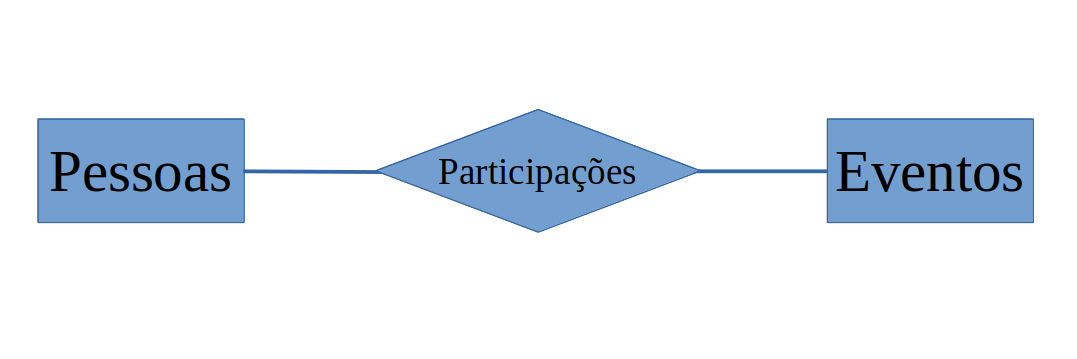
\includegraphics[max size={\textwidth}{\textheight}]{../../imagens/MER-crop.png}

	\end{center}

	\caption{\label{4ad8e04d43602c7274b5a26b3a07d2b00c68d1d7}Diagrama MER do relacionamento Participacoes entre as entidades Pessoas e Eventos. No modelo descritivo o termo relacionamento \'e substitu\'{i}do por associa\c{c}\~ao.}

\end{figure}

Existem relacionamentos (ou associa\c{c}\~oes) que envolvem mais de duas entidades. Daremos um exemplo, aqui, de relacionamento tern\'ario, em que 3 entidades se relacionam por meio de um \'unico relacionamento (associa\c{c}\~ao). Veja na figura XXX como uma rela\c{c}\~ao tern\'aria \'e representada no modelo de abstra\c{c}\~ao conceitual.












\captionsetup{format=plain}
\begin{figure}[htb]

	\begin{center}

		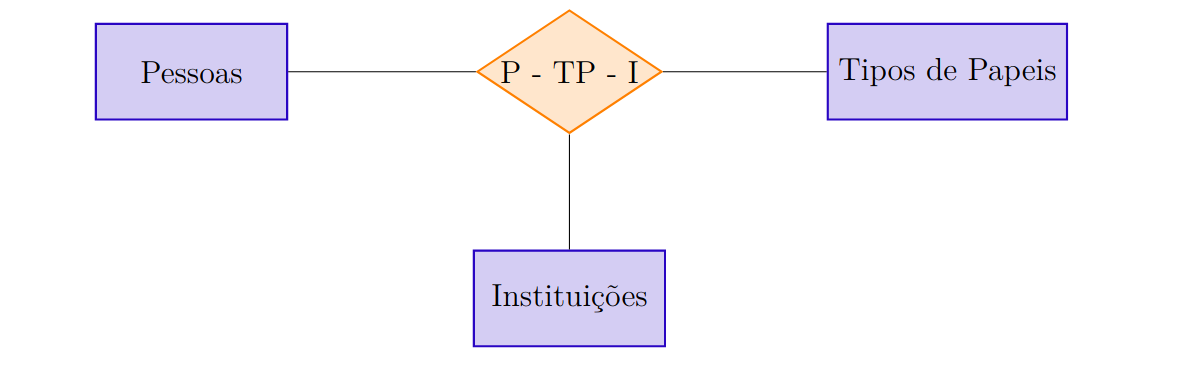
\includegraphics[max size={\textwidth}{\textheight}]{../../imagens/P-TP-I.png}

	\end{center}

	\caption{\label{31147f5e0086cc99f13aad0dd6601e9e784d5117}Representa\c{c}\~ao de uma rela\c{c}\~ao tern\'aria atrav\'es de um diagrama Entidade Relacionamento.}

\end{figure}

Para criar o exemplo da Fig. XXX, em que se v\^e uma rela\c{c}\~ao tern\'aria, consideramos 3 entidades do WASH: \textquotedbl Pessoas\textquotedbl , \textquotedbl Institui\c{c}\~oes\textquotedbl  e \textquotedbl Tipos de Papeis\textquotedbl . \`As vezes \'e dif\'{\i}cil achar um nome curto que represente o relacionamento (ou associa\c{c}\~ao) tern\'ario. Assim, \'e pr\'atica comum usar como nome a sigla constitu\'{\i}da pelas primeiras letras dos nomes das entidades que por meio dele se relacionam. No caso da figura o nome escolhido foi \textquotedbl P-TP-I\textquotedbl .










A entidade \textquotedbl Tipos de Papeis\textquotedbl  representa todos os \textquotedbl tipos de papeis\textquotedbl  que uma pessoa pode desempenhar no Programa WASH. Por exemplo: uma pessoa pode atuar como estudante, como bolsista, como professor ou como orientador, dentre muitas outras possibilidades.










A entidade \textquotedbl Institui\c{c}\~oes\textquotedbl  representa todas as institui\c{c}\~oes que est\~ao envolvidas com atividades do WASH. Por exemplo, podem ser elementos da entidade \textquotedbl Institui\c{c}\~oes\textquotedbl : o Centro de Tecnologia da Informa\c{c}\~ao Renato Archer (CTI), o Instituto Federal de Educa\c{c}\~ao, Ci\^encia e Tecnologia de S\~ao Paulo (IFSP), a Escola Estadual Vitor Meirelles ou o pr\'oprio CNPq.










Uma vez identificadas as 3 entidades da Fig. XXX, podemos entender o relacionamento (ou associa\c{c}\~ao) \textquotedbl P-TP-I\textquotedbl , atrav\'es das seguintes frases em linguagem natural:














\begin{table}[htb]
\tiny
\caption{\label{2dacfd9b77c6bfbbc0b13327966df6d6a3c655fb}Uso de exemplos em linguagem natural para representar a associa\c{c}\~ao P-TP-I.}

\centering
\begin{tabular}{|c|}
\hline
Jo\~ao atua como aluno vinculado ao IFSP \\
Jo\~ao atua como bolsista vinculado ao CNPq \\
Maria atua como orientadora vinculada \`a UNIFESP \\
Maria atua como professora vinculada \`a UNIFESP \\
Pedro atua como coordenador de projeto junto ao CNPq \\
Pedro atua como servidor junto ao CEMADEN \\
\hline
\end{tabular}
\end{table}


\subsection[Business Process Modeling Notation (BPMN)]{Business Process Modeling Notation (BPMN)}\label{Business Process Modeling Notation (BPMN)}
Em elabora\c{c}\~ao.










\section[Fundamenta\c{c}\~ao: caracteriza\c{c}\~ao dos resultados (eixo 3)]{Fundamenta\c{c}\~ao: caracteriza\c{c}\~ao dos resultados (eixo 3)}\label{Fundamenta\c{c}\~ao: caracteriza\c{c}\~ao dos resultados (eixo 3)}
Nesta se\c{c}\~ao ser\'a descrito o embasamento para o trabalho de levantamento de resultados.










\subsection[Indicadores]{Indicadores}\label{Indicadores}
Segundo  Rodrigues (2010)  existe uma \textquotedbl estreita e indissoci\'avel\textquotedbl  rela\c{c}\~ao entre as palavras: medir, informar e \textquotedbl indicador\textquotedbl .










Esta percep\c{c}\~ao de sinon\'{\i}mia fundamenta-se em [apud: [MEADOWS (2006), que aponta a equival\^encia entre os conceitos: sinal, sintoma, press\'agio, aviso, dica, pista, situa\c{c}\~ao, categoria, dados, ponteiro, mostrador, luz de advert\^encia, instrumento e medida.










O termo \textquotedbl indicador\textquotedbl  pode ter um sentido muito mais espec\'{\i}fico quando pensado no contexto gerencial-corporativo (PARMENTER, 2007) ou no contexto de planejamento estrat\'egico, situa\c{c}\~oes que n\~ao est\~ao dentro do escopo desta disserta\c{c}\~ao.










Para esta disserta\c{c}\~ao n\~ao ser\'a explorado o vi\'es corporativo do termo, mas, diferentemente, o sentido de \textquotedbl estat\'{\i}sticas que fornecem algum tipo de medida de um fen\^omeno particular de preocupa\c{c}\~ao\textquotedbl  (apud: WONG, 2006).










Portanto, no contexto deste trabalho, indicadores s\~ao informa\c{c}\~oes quantitativas, que permitem caracterizar os resultados do projeto, tais como:











\begin{alineas}
\item n\'umero de crian\c{c}as atendidas
\item n\'umero de bolsistas
\item n\'umero de relat\'orios
\item distribui\c{c}\~ao de temas abordados em relat\'orios
\item n\'umero de oficinas realizadas
\item distribui\c{c}\~ao et\'aria dos participantes em oficinas
\item temas abordados nas oficinas
\item distribui\c{c}\~ao de temas nas oficinas
\item tipos de atividades realizadas
\item distribui\c{c}\~ao das atividades nas oficinas
\item quantidade de cidades atendidas
\item quantidade de escolas envolvidas
\item quantidade de institui\c{c}\~oes envolvidas
\item quantidade de parlamentares envolvidos
\item participantes mais ass\'{\i}duos
\end{alineas}

Para que os indicadores acima possam ser alcan\c{c}ados \'e preciso uma boa escolha da estrutura\c{c}\~ao de dados, assunto que ser\'a tratado adiante.










\subsection[Informa\c{c}\~ao, dados e conhecimento]{Informa\c{c}\~ao, dados e conhecimento}\label{Informa\c{c}\~ao, dados e conhecimento}
 Setzer e Silva (2017)  nos ensinam a diferen\c{c}a entre:











\begin{alineas}
\item dados
\item informa\c{c}\~oes
\item conhecimento
\end{alineas}

Segundo ele, os \textquotedbl dados\textquotedbl  s\~ao \textquotedbl representa\c{c}\~oes simb\'olicas quantific\'aveis\textquotedbl   (Setzer e Silva, 2017). Como exemplo de dados ele cita as letras do alfabeto. Sempre \'e poss\'{\i}vel atribuir um n\'umero a cada letra. Por exemplo, podemos atribuir o n\'umero 1 \`a letra A, o n\'umero 2 \`a letra B, o n\'umero 3 \`a letra C e assim por diante. Desta forma, um texto pode ser entendido como uma sequ\^encia de n\'umeros e, portanto, no sentido indicado, o texto \'e um dado porque tamb\'em pode ser representado por uma sequ\^encia de n\'umero (a sequ\^encia de n\'umeros que representa a sequ\^encia de letras).










A temperatura de um ambiente tamb\'em \'e um dado: podemos atribuir um n\'umero que indica o valor da temperatura numa determinada escala. Por exemplo, podemos dizer que a sala \textquotedbl est\'a a 35 graus c\'elsius\textquotedbl .










Podemos atribuir um n\'umero para a quantidade de brasileiros e brasileiras, portanto o n\'umero de habitantes do nosso pa\'{\i}s tamb\'em \'e um dado.










Segundo Setzer e Silva (2017) o dado se transforma em \textquotedbl informa\c{c}\~ao\textquotedbl  quando algu\'em \'e capaz de associar um conceito ao dado, estabelecendo uma compreens\~ao humana sobre o que aquele s\'{\i}mbolo quantific\'avel representa.










Desta forma, o dado \textquotedbl temperatura\textquotedbl  s\'o se transforma em informa\c{c}\~ao quando o conceito de \textquotedbl quente\textquotedbl  e \textquotedbl frio\textquotedbl  pode ser associado a ele, numa perspectiva humana.










Ainda segundo Setzer e Silva (2017), as informa\c{c}\~oes se transformam em conhecimento quando os indiv\'{\i}duos s\~ao capazes de estabelecer rela\c{c}\~oes e associa\c{c}\~oes entre as informa\c{c}\~oes.  Setzer e Silva (2017) mencionam a import\^ancia das informa\c{c}\~oes serem adquiridas por uma viv\^encia pessoal para que se tornem conhecimento, caracterizando-o como um atributo subjetivo.










Esta singela defini\c{c}\~ao oferecida por Setzer nos basta para este trabalho, e renunciamos ao tratamento matem\'atico da Teoria da Informa\c{c}\~ao como apresentado por Shannon (Barrios, 2015), por exemplo, uma vez que escapa ao escopo deste estudo.










A defini\c{c}\~ao de Setzer e Silva (2017) \'e corroborada pelo trabalho de MAMMANA (1999), que traz uma interpreta\c{c}\~ao filogen\'etica para o processamento das informa\c{c}\~oes. Esta vis\~ao prop\~oe que \textquotedbl n\~ao existe informa\c{c}\~ao fora da biosfera\textquotedbl  e que a informa\c{c}\~ao seria uma primitiva epistemol\'ogica da biologia. Em outras palavras, os dados representados por s\'{\i}mbolos s\'o adquirem um car\'ater de informa\c{c}\~ao quando passam a influenciar a probabilidade de sobreviv\^encia do patrim\^onio gen\'etico de um indiv\'{\i}duo. Esta vis\~ao fica expl\'{\i}cita na seguinte cita\c{c}\~ao:











\noindent\begin{center}\mbox{\centering\fbox{\centering\par\parbox{0.7\linewidth}{\small\textit{\textquotedbl (...) informa\c{c}\~ao \'e representada pelo aumento de v\'{\i}nculos casuais que constituem os indiv\'{\i}duos (...). Estes v\'{\i}nculos foram constru\'{\i}dos pela evolu\c{c}\~ao e sele\c{c}\~ao natural para melhorar o preparo do indiv\'{\i}duo no enfrentamento dos perigos ambientais e possibilidades, de forma a aumentar a probabilidade de sobreviv\^encia de seus genes.\textquotedbl  (tradu\c{c}\~ao livre de  MAMMANA (1999))}\normalsize}}}\end{center}


Segundo essa vis\~ao de  MAMMANA (1999), que suplementa a vis\~ao de Shannon baseada na entropia, uma cadeia de processos de de-somatiza\c{c}\~ao de habilidades humanas evolui para extens\~ao do papel evolutivo da informa\c{c}\~ao para o contexto antropol\'ogico e cultural.










Uma vis\~ao alternativa sobre como fazer uma distin\c{c}\~ao entre informa\c{c}\~ao e conhecimento \'e apresentada por  VITAL e CAF\'E (2011), citando Fogl (1979). Nesta vis\~ao, o conhecimento \'e um dos elementos da informa\c{c}\~ao, que conteria (VITAL e CAF\'E, 2011):











\begin{alineas}
\item Conhecimento (conte\'udo da informa\c{c}\~ao)
\item linguagem (um instrumento de express\~ao de itens de informa\c{c}\~ao) e
\item suporte (objetos, materiais e energia)
\end{alineas}

Desta forma, segundo Fogl  (Apud, VITAL e CAF\'E, 2011) , \textquotedbl o conhecimento materializa-se na informa\c{c}\~ao, atrav\'es de seu conte\'udo\textquotedbl . Essa vis\~ao traz o conhecimento como resultado da cogni\c{c}\~ao, sendo \textquotedbl o conte\'udo ideal da consci\^encia humana\textquotedbl , ao passo que e informa\c{c}\~ao \'e uma forma material da exist\^encia do conhecimento. Assim, a informa\c{c}\~ao seria o conhecimento expresso por algum \textquotedbl sistema de signos percebidos pelos \'org\~aos e sentidos\textquotedbl , a exemplo da linguagem natural  (VITAL e CAF\'E, 2011).










No contexto do Programa WASH \'e preciso identificar quais dados e suas combina\c{c}\~oes, na forma de informa\c{c}\~oes, t\^em relev\^ancia para a exist\^encia e reprodu\c{c}\~ao do projeto ao longo dos anos. Portanto \'e a identifica\c{c}\~ao desta relev\^ancia que definir\'a quais s\~ao as informa\c{c}\~oes que dele precisam ser extra\'{\i}das, com vistas \`a sua caracteriza\c{c}\~ao.










O Programa WASH \'e prof\'{\i}cuo na produ\c{c}\~ao de dados, uma vez que atende uma quantidade muito grande de crian\c{c}as, adolescentes e adultos. Estes dados est\~ao distribu\'{\i}dos em v\'arias localidades e se referem \`as atividades realizadas em institui\c{c}\~oes de variados tipos, cujas estruturas s\~ao muito diferentes uma das outras. Os tipos de atividades s\~ao muito variados, dependendo das caracter\'{\i}sticas locais, bem como os temas que s\~ao abordados.










Como se ver\'a adiante, o WASH ocorre  em escolas fundamentais, m\'edias, t\'ecnicas, organiza\c{c}\~oes sociais, sindicatos, igrejas, centros de inclus\~ao social p\'ublicos, centros de pesquisa, universidades, em feiras e exposi\c{c}\~oes, dentre tantas outras modalidades.










O formato do WASH \'e variado, podendo ocorrer no contexto escolar, no contra-turno, presencialmente ou remotamente.










Muito embora seja um requisito a promo\c{c}\~ao dos valores do m\'etodo cient\'{\i}fico, o WASH tamb\'em \'e plural no que se refere \`a suas tem\'aticas e o tipos de atividades que s\~ao realizadas.










A diversidade de institui\c{c}\~oes envolvidas, de formatos de realiza\c{c}\~ao, de tem\'aticas, de localidades e de tipos de atividades imp\~oe um desafio sobre como os dados devem ser estruturados, para que representem a ess\^encia do projeto, convers\'{\i}vel em informa\c{c}\~oes \'uteis para a gest\~ao, reprodu\c{c}\~ao e longevidade do mesmo.










Esta forma de estrutura\c{c}\~ao dos dados define como ser\~ao gerados os indicadores de interesse para a caracteriza\c{c}\~ao do projeto, estabelecendo o n\'{\i}vel de confian\c{c}a na sua capacidade de representar essas caracter\'{\i}sticas.










\subsection[Registro de dados na escola p\'ublica]{Registro de dados na escola p\'ublica}\label{Registro de dados na escola p\'ublica}
Visando compreender as alternativas para determinar a quantidade de participantes, bem como outros indicadores no \^ambito do Programa WASH, h\'a que se olhar brevemente para como a escola p\'ublica regula sua pr\'opria armazenagem de dados. Al\'em disso, \'e preciso compreender preliminarmente a forma como o WASH funciona, tema que ser\'a muito mais detalhado na parte de resultados.










A primeira caracter\'{\i}stica do Programa WASH que determina a forma como a coleta de dados precisar\'a ser feita, e que podemos antecipar neste ponto do texto, \'e sua diferen\c{c}a em rela\c{c}\~ao a outros programas de bolsas de inicia\c{c}\~ao cient\'{\i}fica.










Diferentemente de programas que ocorrem no \^ambito acad\^emico de pesquisa, o Programa WASH tem uma \^enfase maior em extens\~ao, que deve ser concretizada pela oferta de oficinas em STEAM para o ensino fundamental. Na pr\'atica, isso significa que os bolsistas participantes do WASH precisam realizar oficinas nas escolas p\'ublicas e outros tipos de entidade, em temas variados, promovendo atividades diversas, com cronogramas que s\~ao articulados caso a caso, uma vez que precisam se adaptar nas necessidades da escola. Estas caracter\'{\i}sticas geram uma complexidade maior do modelo de representa\c{c}\~ao de dados do que aquele que seria necess\'ario para uma escola regular.










Com esta complexidade em mente, \'e preciso criar meios de coletar dados sobre, principalmente:











\begin{alineas}
\item o n\'umero de crian\c{c}as atendidas,
\item n\'umero de oficinas ofertadas
\item n\'umero de institui\c{c}\~oes participantes
\item n\'umero de horas de atividade por estudante
\item cidades atendidas
\item frequ\^encia dos bolsistas multiplicadores
\item distribui\c{c}\~ao et\'aria dos participantes
\end{alineas}

dentre tantos.










A forma plural como o Programa WASH busca atender seus benefici\'arios ficar\'a mais clara adiante, mas neste ponto podemos dizer que o WASH tamb\'em \'e bastante diferente de uma escola do ensino formal, na qual est\~ao bem estabelecidas as normas de participa\c{c}\~ao de estudantes, bem como as regras para o registro da frequ\^encia dos participantes.










Por ser um programa sem uma legisla\c{c}\~ao espec\'{\i}fica para o estabelecimento de obriga\c{c}\~oes entre os part\'{\i}cipes, o WASH tem que ocorrer no \^ambito de organiza\c{c}\~oes (escolas, associa\c{c}\~oes, igrejas, sindicatos) que j\'a seguem normas voltadas para garantir a prote\c{c}\~ao dos menores de idade.










Portanto, outra caracter\'{\i}stica do sistema de registro de participa\c{c}\~oes de estudantes do WASH \'e ser flex\'{\i}vel o bastante para garantir a representa\c{c}\~ao desse ambiente diverso institucionalmente, adaptando-se \`a realidade de cada institui\c{c}\~ao parceira.










Podemos exemplificar o n\'{\i}vel de normatiza\c{c}\~ao da escola p\'ublica regular usando o caso do Estado de S\~ao Paulo, que, como em outros estados, tem legisla\c{c}\~ao espec\'{\i}fica detalhada sobre como registrar a presen\c{c}a de seus alunos.










Escolhemos a vers\~ao de 2010 da \textquotedbl LEGISLA\c{C}\~AO DE ENSINO FUNDAMENTAL E M\'EDIO ESTADUAL\textquotedbl  do Estado de S\~ao Paulo como exemplo, para mostrar que o controle de frequ\^encia de alunos \'e normatizado por meio do Art. 6o da RESOLU\c{C}\~AO SE No 20, DE 17 DE FEVEREIRO DE 2010, in verbis:











\noindent\begin{center}\mbox{\centering\fbox{\centering\par\parbox{0.7\linewidth}{\small\textit{Artigo 6º – Cabe aos professores manter atualizados os dados de frequ\^encia e avalia\c{c}\~ao dos alunos nos respectivos di\'arios de classe, a fim de subsidiar o seu registro e atualiza\c{c}\~ao, no Sistema.}\normalsize}}}\end{center}


Em outros pontos essa legisla\c{c}\~ao traz mais detalhes sobre como esse registro deve ser feito.










Como se v\^e, pela import\^ancia que tem na medi\c{c}\~ao da efici\^encia e efic\'acia da presta\c{c}\~ao do servi\c{c}o de educa\c{c}\~ao, o controle de presen\c{c}a \'e instrumento regulamentado e com atribui\c{c}\~ao de responsabilidades espec\'{\i}ficas no \^ambito da Secretaria Estadual de Educa\c{c}\~ao de S\~ao Paulo, assim como ocorre em outros estados.










Al\'em de servir de indicador de efici\^encia e efic\'acia, o controle de frequ\^encia tamb\'em funciona como auxiliar das tarefas log\'{\i}sticas e de planejamento da escola. Com o controle de presen\c{c}a \'e poss\'{\i}vel saber quais escolas devem receber mais recursos, por exemplo, e uma falha na gera\c{c}\~ao destes dados pode comprometer a qualidade de todo o servi\c{c}o.










O WASH, por ser uma atividade de educa\c{c}\~ao complementar \`a da escola regular, n\~ao tem uma normatiza\c{c}\~ao equivalente. Mesmo assim n\~ao pode abrir m\~ao de produzir seus pr\'oprios indicadores de efici\^encia e efic\'acia, raz\~ao pela qual  precisou desenvolver um m\'etodo pr\'oprio.










Essa necessidade de um sistema pr\'oprio de registro decorre da impossibilidade de compartilhamento ostensivo de dados por parte das institui\c{c}\~oes respons\'aveis pelos alunos. Em algumas situa\c{c}\~oes, como \'e o caso de atividades realizadas em associa\c{c}\~oes e igrejas, por exemplo, a institui\c{c}\~ao parceira sequer tem um sistema otimizado de controle de presen\c{c}a, fato que refor\c{c}a a necessidade do WASH criar seus pr\'oprios m\'etodos de gera\c{c}\~ao de indicadores.










Esta necessidade de registro foi reconhecida nos prim\'ordios do Projeto e uma descri\c{c}\~ao da evolu\c{c}\~ao dos m\'etodos de coleta de dados \'e feita no Resultados e An\'alise desta disserta\c{c}\~ao.










\subsection[Investimento por educando: escola p\'ublica vs. privada]{Investimento por educando: escola p\'ublica vs. privada}\label{Investimento por educando: escola p\'ublica vs. privada}
MAMMANA et al. (2020)  apresentam, atrav\'es da tabela XXX, um c\'alculo do investimento por estudante, por hora, com base em dados do Fundeb, comparando-o com o que \'e investido em alunos das escolas privadas. Na tabela usamos os seguintes c\'odigos: EF (ensino fundamental), PS (primeiras s\'eries) e TN (todos os n\'{\i}veis).














\begin{table}[htb]
\tiny
\caption{\label{02a61f21bf9049ea550d07c2199237e202a09ecd}Compara\c{c}\~ao do investimento por hora por aluno nas escolas privadas e p\'ublicas. Os dados t\^em origem em v\'arias fontes regionais: Fundeb, DOU e Plataforma Campineira Melhor Escola. (Fonte:  [[MAMMANA et al. (2020)]])}

\centering
\begin{tabular}{|c|c|c|c|c|c|}
\hline
Tipo  &  Fonte  &  N\'{\i}vel  &  \'Area  &  Reais por aluno por ano  &  Reais por hora por aluno \\
\hline
P\'ublica  &  Fundeb 2006  &  EF/PS  &  Urbana  &  3,3 mil  &  4,12 \\
P\'ublica  &  Fundeb 2006  &  EF/PS  &  Rural  &  3,8 mil  &  4,75 \\
P\'ublica  &  DOU 2006  &  TN  &  Nordeste  &  2,7 mil  &  3,37 \\
Priv. Alto Padr\~ao  &  Estimativa  &  TN  &  Urbana  &  48 mil  &  60,00 \\
Priv. M\'edio Padr\~ao  &  Plat. Melhor Escola  &  TN  &  Urbana  &  13,3 mil  &  16,70 \\
\hline
\end{tabular}
\end{table}


Para o c\'alculo de investimento por hora, por aluno,  MAMMANA et al. (2020) consideraram que um ano letivo tem 200 dias e que a crian\c{c}a \'e exposta a 4 horas di\'arias de atividades escolares.










Os dados mostram que o setor p\'ublico tem investido menos de 1 d\'olar por hora, por aluno. Esse n\'umero \'e cerca de 4 a 5 vezes menor do que \'e investido pelas fam\'{\i}lias numa crian\c{c}a que frequenta escola privada de classe m\'edia no interior de S\~ao Paulo e cerca de 10 vezes menor do que o investido por fam\'{\i}lias de alta renda  (MAMMANA et al., 2020).











\noindent\begin{center}\mbox{\centering\fbox{\centering\par\parbox{0.7\linewidth}{\small\textit{\textquotedbl Estes dados mostram uma situa\c{c}\~ao de apartheid que pode aprofundar ainda mais o desequil\'{\i}brio de oportunidades entre estudantes mais e menos abastados, principalmente quando se considera que todos experimentar\~ao, em desigualdade de condi\c{c}\~oes, os processos seletivos nacionais uniformizados para ingresso no ensino superior\textquotedbl  (Fonte:  MAMMANA et al. (2020))}\normalsize}}}\end{center}


\subsection[Planilhas eletr\^onicas para registro de dados]{Planilhas eletr\^onicas para registro de dados}\label{Planilhas eletr\^onicas para registro de dados}
As planilhas eletr\^onicas s\~ao softwares que permitem guardar  dados e realizar opera\c{c}\~oes com eles num formato de tabela, com o objetivo de lhes extrair informa\c{c}\~oes.










A planilha eletr\^onica \'e um dos m\'etodos mais populares para armazenagem e an\'alise de dados porque tem uma curva de aprendizado relativamente favor\'avel. Em outras palavras, com pouca capacita\c{c}\~ao \'e poss\'{\i}vel obter resultados rapidamente.










O Programa WASH iniciou sua armazenagem de dados empregando planilhas eletr\^onicas justamente por conta desta facilidade, mas t\~ao r\'apido quanto os primeiros resultados come\c{c}aram a aparecer, tamb\'em come\c{c}aram a ficar evidentes as limita\c{c}\~oes deste m\'etodo, embora ainda existam no projeto muitos dados que permanecem sendo armazenados em planilhas. Ali\'as, utilizamo-nos de planilhas para verifica\c{c}\~ao de dados que j\'a est\~ao estruturados em Bancos de Dados Relacionais, como se ver\'a nos Resultados e An\'alise. Por ora este assunto n\~ao ser\'a tratado aqui.










Com base nesta observa\c{c}\~ao de dificuldades, o foco aqui ser\'a embasar, por compara\c{c}\~ao, a decis\~ao de empregar a modelagem relacional, em detrimento de outros m\'etodos menos estruturados, como \'e o caso das planilhas eletr\^onicas. A modelagem relacional ser\'a tratada na pr\'oxima se\c{c}\~ao como solu\c{c}\~ao para algumas das dificuldades que ser\~ao tratadas na presente se\c{c}\~ao.










De forma bem suscinta, podemos recapitular que a coleta de dados de presen\c{c}a no \^ambito do Programa WASH se deu, inicialmente, por meio que podemos chamar de anal\'ogico: o registro em papel do nome das crian\c{c}as presentes, com a marca\c{c}\~ao da data e caracter\'{\i}sticas dos eventos no topo da folha.










Com o crescimento r\'apido do projeto, este m\'etodo come\c{c}ou a ficar invi\'avel e foi tentada a utiliza\c{c}\~ao de formul\'arios on-line tipo \textquotedbl Google Forms\textquotedbl , os quais eram transferidos para planilhas eletr\^onicas visando armazenagem.










O emprego de planilhas eletr\^onicas tamb\'em se mostrou insatisfat\'orio e \'e neste ponto que come\c{c}amos a revis\~ao da literatura sobre o assunto.










FULLER (2011), em seu artigo \textquotedbl Vantagens e perigos de usar o Microsoft Excel para organizar e apresentar dados de qualidade de \'agua\textquotedbl  (tradu\c{c}\~ao livre do t\'{\i}tulo) nos presenteia com algumas importantes reflex\~oes:











\noindent\begin{center}\mbox{\centering\fbox{\centering\par\parbox{0.7\linewidth}{\small\textit{Usar o Excel para organizar os dados \'e uma tremenda vantagem, mas tamb\'em cria oportunidade para introduzir erros insidiosos no conjunto de dados, erros que podem entrar nos dados de forma sutil, com impacto pervasivo mas muito dif\'{\i}cies de descobrir(...) (tradu\c{c}\~ao livre de FULLER (2011))}\normalsize}}}\end{center}


O n\'{\i}vel de confian\c{c}a nesta afirma\c{c}\~ao de  FULLER (2011) \'e bastante alto, uma vez que o trabalho de coleta de dados por ele realizado envolveu a entrada de uma m\'edia de 4.752 dados anuais por mais de 10 anos, o que certamente permitiu que ele avaliasse a confiabilidade do Excel como ferramenta. A escolha do Excel como ferramenta em sua pesquisa fora aprovada pela Ag\^encia de Fomento  (FULLER, 2011), uma transi\c{c}\~ao do m\'etodo anterior de coleta, que segundo ele era baseado em planilhas em papel com c\'alculos feitos em calculadora.










Apenas para registro, no sentido de prover uma melhor figura sobre o que esta refer\^encia pode nos trazer, cabe mencionar que os dados envolviam data de coleta, hor\'ario, condi\c{c}\~oes meteorol\'ogicas, temperatura do ar, pH, condutividade, condut\^ancia espec\'{\i}fica e oxig\^enio dissolvido.










Com base nesta vasta experi\^encia,  FULLER (2011) identificou as seguintes fontes de erros na entrada de dados:











\begin{alineas}
\item Erros de digita\c{c}\~ao: normalmente envolviam apertar inadvertidamente n\'umeros adjacentes no teclado, ou simplesmente ler os dados de laborat\'orio de forma errada. Esse tipo de erro pode alterar dramaticamente as m\'edias e passar despercebido nos gr\'aficos de espalhamento de dados.
\item Deslocamento de colunas e repeti\c{c}\~ao inadvertida de dados: algumas vezes uma coluna pode ser repetida sem que a pessoa respons\'avel por entrar os dados perceba, por exemplo.
\item Perda de n\'umeros ou multiplicidade indevida de entrada de dados: isto pode gerar uma coluna de dados com menos ou mais dados do que o n\'umero original, causando um deslocamento nos dados.
\end{alineas}

Estes tipos de erro, por mais pros\'aicos que possam parecer, tinham paralelo na experi\^encia de registro do WASH por n\'os vivenciada. No in\'{\i}cio do projeto observaramos uma falta de qualidade dos dados de presen\c{c}a de crian\c{c}as do ensino fundamental no WASH, uma situa\c{c}\~ao que requeria medidas por parte da equipe de gest\~ao do projeto.










 Brudner (2022) complementa essa vis\~ao, mas com uma abordagem mais de neg\'ocios, trazendo as vantagens e desvantagens na utiliza\c{c}\~ao de planilhas eletr\^onicas.










Dentre as vantagens podemos citar (Brudner, 2022) e comentar, como segue:











\begin{alineas}
\item as planilhas eletr\^onicas podem ser obtidas gratuitamente, a exemplo do LibreOffice e do Google Docs. Mesmo empresas como a Microsoft oferecem acesso gratuito a algumas de suas vers\~oes.
\item as planilhas eletr\^onicas requerem pouco treinamento para seu uso b\'asico
\item planilhas eletr\^onicas s\~ao \textquotedbl customiz\'aveis\textquotedbl , ou seja, permitem ser configuradas facilmente para atender aquela necessidade espec\'{\i}fica do usu\'ario
\item as planilhas eletr\^onicas permite o trabalho colaborativo, quando muitos usu\'arios editam a planilha ao mesmo tempo. Essa possibilidade tamb\'em pode ser um problema, dado que pode resultar em re-trabalho quando um usu\'ario modifica os dados j\'a verificados por outro, por exemplo
\item as planilhas eletr\^onicas permitem uma manipula\c{c}\~ao e an\'alise de dados relativamente f\'acil, o que tamb\'em pode ser um problema, dado que \'e f\'acil remover parte dos dados, tornando-os n\~ao confi\'aveis
\item as planilhas s\~ao facilmente integr\'aveis com outras  ferramentas, mesmo com banco de dados especializados
\item as planilhas s\~ao facilmente integr\'aveis ao fluxo de trabalho de sua equipe, n\~ao requerendo custosas adapta\c{c}\~oes, como \'e o caso de sistemas menos flex\'{\i}veis
\item as planilhas geram facilmente documentos de grande apelo visual, principalmente no ambiente de neg\'ocios. H\'a uma grande quantidade de \textquotedbl templates\textquotedbl  que d\~ao bastante flexibilidade para a apresenta\c{c}\~ao dos resultados.
\end{alineas}

 Brudner (2022) tamb\'em aponta as desvantagens das planilhas eletr\^onicas, as quais s\~ao comentadas abaixo:











\begin{alineas}
\item embora f\'aceis de usar, as planilhas s\~ao desajeitadas, principalmente quando \'e preciso manipular grandes quantidades de dados. O usu\'ario se ver\'a percorrendo (scrolling) e inspecionando centenas ou at\'e milhares de c\'elulas para poder encontrar seus dados, mesmo quando tem ferramentas de busca e filtros dispon\'{\i}veis.
\item as planilhas eletr\^onicas n\~ao s\~ao seguras, dado que n\~ao t\^em sistemas de autentica\c{c}\~ao (login). Uma vez distribu\'{\i}das, colocam em risco a privacidade das pessoas ali registradas (no caso de registros de presen\c{c}a), uma fragilidade frente aos requisitos da Lei Geral de Prote\c{c}\~ao de Dados, por exemplo.
\item a facilidade com que as planilhas eletr\^onicas podem ser utilizadas de forma colaborativa cria um outro problema: \'e dif\'{\i}cil dizer quem editou os dados pela \'ultima vez. Isso prejudica a rastreabilidade dos erros, dificultando sua corre\c{c}\~ao. Quando muitas pessoas entram dados, como \'e o caso do WASH, \'e comum um usu\'ario inadvertidamente introduzir erros em cima do trabalho de outro, os quais depois ser\~ao muito dif\'{\i}ceis de encontrar.
\item as planilhas eletr\^onicas criam v\'arias vers\~oes da mesma \textquotedbl verdade\textquotedbl   (Brudner, 2022), mesmo que todos os usu\'arios de dados partam da mesma fonte de dados inicial. Isso ocorre porque \'e comum os usu\'arios salvarem suas pr\'oprias vers\~oes da planilha, criando um problema de concorr\^encia de atualiza\c{c}\~oes.
\item da mesma forma como  FULLER (2011),  Brudner (2022) tamb\'em aponta a inevitabilidade de erros introduzidos pelos v\'arios usu\'arios.
\item muito embora as planilhas permitam obter relat\'orios rapidamente para estruturas simples, \`a medida que as estruturas v\~ao ficando mais complexas, torna-se cada vez mais dif\'{\i}cil gerar novos relat\'orios
\item o fato das planilhas serem \textquotedbl customiz\'aveis\textquotedbl  e independentes de uma equipe de suporte tamb\'em significa que o pr\'oprio usu\'ario tem que gerar seus gr\'aficos, o que consume bastante tempo e pode ser bastante frustrante quando n\~ao se consegue obter a vis\~ao desejada
\item al\'em da falta de seguran\c{c}a em termos de expor a privacidade das pessoas registradas, as planilhas s\~ao particularmente propensas a perder dados, seja por erros de opera\c{c}\~ao ou por problemas com os sistemas de armazenamento, uma vez que as planilhas n\~ao tem sistemas robustos de \textquotedbl back-up\textquotedbl 
\item \`a medida que o seu \textquotedbl neg\'ocio\textquotedbl  se amplia e os requisitos de tratamento de dados v\~ao se tornando mais complexos, \'e natural que sistemas especializados sejam necess\'arios, situa\c{c}\~ao que nem sempre permite a integra\c{c}\~ao dos dados antigos, presentes na planilha eletr\^onica
\item as planilhas eletr\^onicas n\~ao podem ser integradas a aplicativos mobile, dificultando a ubiquicidade
\end{alineas}

N\~ao obstante as vantagens, o fato \'e que todas estas desvantagens mostraram-se determinantes no caso do Programa WASH, requerendo uma a\c{c}\~ao no sentido de buscar formas mais robustas de armazenagem.










Mostraremos, agora, algumas situa\c{c}\~oes que ocorrem em planilhas eletr\^onicas que acabam prejudicando a confiabilidade nos dados.










Vamos considerar uma representa\c{c}\~ao de uma planilha eletr\^onica na forma de uma tabela de cadastro de estudantes.










Na representa\c{c}\~ao, cada linha \'e o cadastro de uma estudante e seus dados est\~ao dispostos em colunas, como segue:














\begin{table}[htb]
\tiny
\caption{\label{ddd7a335bbc10f88eaaf4abda266d151f0ba0e6f}Exemplo de cadastro de estudantes armazenado em planilha eletr\^onica.}

\centering
\begin{tabular}{|c|c|c|c|c|}
\hline
  &  A  &  B  &  C  &  D  \\
\hline
0 & Nome  &  Cidade  &  Data de Nascimento  &  Escola \\
1 & Jos\'e  &  Campinas  &  10/10/2010  &  Bento \\
2 & Maria  &  Cmpinas  &  03/04/2012  &  Bento \\
3 & Jo\~ao  &  S\~ao Paulo  &  11/12/2004  &  Bento \\
4 & M\'ario  &  S. Paulo  &  30/01/2009  &  Bento \\
5 & Pedro  &  Sao Paulo  &  13/02/2013  &  Bento \\
\hline
\end{tabular}
\end{table}


Na tabela que representa a planilha vemos um tipo de erro de prenchimento muito comum, que \'e a falta de uniformiza\c{c}\~ao da representa\c{c}\~ao dos dados.










Veja, por exemplo, o nome da cidade na c\'elula B2, que est\'a grafada errado (Cmpinas, quando deveria ser Campinas). Esse \'e um erro t\'{\i}pico de digita\c{c}\~ao, quando a pessoa respons\'avel por entrar o dado esquece uma letra.










Tamb\'em na linha da falta de uniformiza\c{c}\~ao, vemos a situa\c{c}\~ao das c\'elulas B3, B4 e B5. Ali a cidade \textquotedbl S\~ao Paulo\textquotedbl  est\'a grafada de 3 formas diferentes: S\~ao Paulo, S. Paulo e Sao Paulo. N\~ao \'e um erro de digita\c{c}\~ao, mas simplesmente a falta de um acordo pr\'evio sobre como a palavra S\~ao Paulo deve ser grafada. Podemos imaginar uma situa\c{c}\~ao em que v\'arias pessoas preencheram informa\c{c}\~oes na planilha, cada uma com uma pr\'atica de grafia diferente da palavra S\~ao Paulo.










Esta falta de uniformiza\c{c}\~ao, seja por um erro ou por diferentes pr\'aticas de representa\c{c}\~ao dos dados, causa muitos problemas para a obten\c{c}\~ao de informa\c{c}\~oes a partir dos dados. No exemplo, pode ser interpretado que o Projeto tem apenas 1 pessoa da cidade de S\~ao Paulo, caso a busca por paulistanos se d\^e a partir da grafia \textquotedbl S\~ao Paulo\textquotedbl . Da mesma forma, pode ser interpretado que h\'a apenas uma pessoa da cidade de Campinas, caso a busca se d\^e pela grafia \textquotedbl Campinas\textquotedbl . Numa planilha pequena, com poucas linhas, \'e evidente que este tipo de erro \'e f\'acil de perceber. Mas em planilhas com grande quantidade de dados esse erro pode ser muito dif\'{\i}cil de detectar.










As planilhas eletr\^onicas t\^em meios de diminuir a chance desse problema ocorrer. Uma das formas \'e o auto-preenchimento, uma facilidade que usa a informa\c{c}\~ao das c\'elulas anteriores daquela coluna para sugerir um preenchimento para o usu\'ario. Mas esta facilidade n\~ao \'e auto-consistente e o usu\'ario pode n\~ao aceitar a sugest\~ao, criando o erro.










O exemplo de planilha eletr\^onica abaixo mostra outro tipo de problema de preenchimento comum a esta ferramenta:














\begin{table}[htb]
\tiny
\caption{\label{f6feaa39313aa0691b7fdadc84175a203e68bf77}Deslocamento para esquerda de um conjunto de c\'elulas de uma planilha eletr\^onica}

\centering
\begin{tabular}{|c|c|c|c|c|}
\hline
  &  A  &  B  &  C  &  D  \\
0 & Nome  &  Cidade  &  Data de Nascimento  &  Escola \\
1 & Jos\'e  &  10/10/2010  &  Bento  &   \\
2 & Maria  &  Cmpinas  &  03/04/2012  &  Bento \\
3 & Jo\~ao  &  S\~ao Paulo  &  11/12/2004  &  Bento \\
4 & M\'ario  &  S. Paulo  &  30/01/2009  &  Bento \\
5 & Pedro  &  Sao Paulo  &  13/02/2013  &  Bento \\
\hline
\end{tabular}
\end{table}


No segundo exemplo de planilha eletr\^onica vemos uma situa\c{c}\~ao de erro de preenchimento bastante comum: deslocar os dados de uma linha para a esquerda, apagando indevidamente uma c\'elula. Este tipo de erro ocorre na planilha porque ela n\~ao verifica o tipo de dado que est\'a sendo colocado numa dada c\'elula. Por exemplo, com o deslocamento para a esquerda, a c\'elula que cont\'em o nome da escola D1 acaba por preencher a c\'elula C1, que deveria ser do tipo data, mas que agora cont\'em uma sequ\^encia de letras \textquotedbl Bento\textquotedbl . Novamente, \'e um erro f\'acil de perceber em planilhas pequenas, mas que pode causar muito estrago e ser dif\'{\i}cil de perceber quando temos milhares de linhas numa planilha.










Neste ponto podemos nos perguntar: ser\'a que existe alguma tecnologia que garanta a consist\^encia dos dados a qualquer momento, evitando que o usu\'ario consiga entrar dados de forma a prejudicar a integridade da base de dados?










Esta tecnologia se chama \textquotedbl Banco de Dados Relacional\textquotedbl , que ser\'a descrita na pr\'oxima se\c{c}\~ao.










\subsection[Bancos de Dados Relacionais]{Bancos de Dados Relacionais}\label{Bancos de Dados Relacionais}
A teoria por tr\'as de Bancos de Dados Relacionais \'e bastante sofisticada envolvendo uma \'Algebra que escapa aos objetivos desta disserta\c{c}\~ao. Entretanto alguns elementos s\~ao f\'aceis de compreender e podem ser expostos aqui de uma forma simples o suficiente para atender ao objetivo de justificar as escolhas feitas ao longo deste trabalho. Isto pode ser feito sem preju\'{\i}zo para o rigor e erudi\c{c}\~ao cient\'{\i}ficos.










O pioneiro na cria\c{c}\~ao dos conceitos de Bancos de Dados Relacionais foi Edgard Codd, um pesquisador da IBM que revolucionou a forma como o mundo passou a armazenar dados. Seu paper seminal foi  \textquotedbl A Relational Model of Data for Large Shared Data Banks\textquotedbl  de 1970, um marco na \'area (CODD, 1970). Ao longo de sua vida, Codd lutou contra uma resist\^encia para implanta\c{c}\~ao de suas ideias dentro da pr\'opria IBM, a qual tinham origem em interesses comerciais, uma vez que a IBM j\'a tinha sistemas implantados baseados em outras formas de representa\c{c}\~ao de dados, e n\~ao tinha interesse em uma nova solu\c{c}\~ao concorrente. O modelo de Codd, muito superior, passou a ser considerado pela IBM por conta da press\~ao de concorrentes e de seus clientes, que passaram a exigir uma solu\c{c}\~ao baseada nas ideias de Codd.










A for\c{c}a das ideias de Codd pode ser percebida na seguinte transcri\c{c}\~ao de seu artigo seminal (CODD, 1970):











\noindent\begin{center}\mbox{\centering\fbox{\centering\par\parbox{0.7\linewidth}{\small\textit{A vis\~ao ou modelo relacional de dados descrita na se\c{c}\~ao 1 parece ser superior, em v\'arios aspectos, quando comparada com os modelos de grafo e de rede [3,4] presentemente em voga para sistemas n\~ao inferenciais. Ela prov\^e meios para descrever dados com estrutura puramente natural, ou seja, sem a super imposi\c{c}\~ao de uma estrutura adicional para a representa\c{c}\~ao dos dados na m\'aquina. Assim, obt\'em-se as bases para uma linguagem de dados de alto n\'{\i}vel, que prov\^e a m\'axima independ\^encia entre programas de um lado e a representa\c{c}\~ao e organiza\c{c}\~ao dos dados de outro. (Tradu\c{c}\~ao Livre de  CODD (1970))}\normalsize}}}\end{center}


A frase acima indica uma busca por uma representa\c{c}\~ao dos dados que fosse independente da representa\c{c}\~ao espec\'{\i}fica numa m\'aquina em particular. Ou seja, Codd buscou uma forma de abstrair a representa\c{c}\~ao dos dados, sem ter que se preocupar como a m\'aquina os guardava, criando a possibilidade de independ\^encia do tipo de computador, sistema operacional ou at\'e do tipo de software de gest\~ao de dados. Isto tornou a armazenagem de dados muito mais flex\'{\i}vel, robusta e auto-consistente. Por auto-consistente podemos entender dados que dificilmente poder\~ao sofrer corrup\c{c}\~oes, porque o pr\'oprio sistema \'e preparado para evitar dados n\~ao consistentes.










Para garantir a funcionalidade de seu esquema de armazenagem, Codd pensou em \textquotedbl regras\textquotedbl  ou normas.










Frequentemente s\~ao referidas 12 normas para caracterizar a formaliza\c{c}\~ao de Codd, mas identificamos muitas varia\c{c}\~oes na forma de apresentar essas regras, a exemplo do que oferece Setzer e Silva (2017).










Assim, buscamos criar a nossa pr\'opria compreens\~ao das regras de Codd, integrando conhecimentos presentes no artigo de  CODD (1970) e  Setzer e Silva (2017), conhecimentos presentes em Wikipedia\_Codd (2022),  TutorialsPoint (2022) e  RelDB (2019). Portanto estamos combinando fontes can\^onicas, a exemplo de  CODD (1970) e Setzer e Silva (2017), com outras mais heterod\'oxicas, o que \'e perfeitamente plaus\'{\i}vel no caso, uma vez que n\~ao se trata de especialidade da autora, mas instrumental para justificar algumas decis\~oes tomadas ao longo deste trabalho.










Para come\c{c}ar a compreender os Bancos de Dados relacionais, vamos aceitar uma regra fundamental desse esquema que \'e:











\noindent\begin{center}\mbox{\centering\fbox{\centering\par\parbox{0.7\linewidth}{\small\textit{Toda informa\c{c}\~ao num Banco de Dados Relacional \'e representada exclusivamente por meio de tabelas, com linhas e colunas (adaptado de RelDB (2019))}\normalsize}}}\end{center}


Num primeiro momento, analisada isoladamente, esta regra pode confundir as pessoas, levando-as a pensar que, como as planilhas eletr\^onicas s\~ao tabelas, elas tamb\'em s\~ao bancos de dados relacionais, mas isto n\~ao \'e verdade, como ficar\'a claro pelas demais regras.










Posto isto, vamos ver o que \'e uma tabela dentro do conceito de Bancos de Dados relacionais:














\begin{table}[htb]
\tiny
\caption{\label{f66c1ac239a347d2b455611f794c18300b1974b6}Exemplo de tabela de um banco de dados relacional: cadastro de pessoas.}

\centering
\begin{tabular}{|c|c|c|c|}
\hline
Nome  &  Cidade  &  Data de Nascimento  &  Escola \\
Jos\'e  &  Campinas  &  10/10/2010  &  Bento \\
Maria  &  Campinas  &  03/04/2012  &  Bento \\
Jo\~ao  &  Campinas  &  11/12/2004  &  Bento \\
M\'ario  &  Campinas  &  30/01/2009  &  Bento \\
Pedro  &  Campinas  &  13/02/2013  &  Bento \\
\hline
\end{tabular}
\end{table}


Como se v\^e, uma tabela no sentido de banco de dados relacionais \'e exatamente o que vem \`a mente quando uma pessoa sem forma\c{c}\~ao na \'area imagina: um conjunto de linhas e colunas que se cruzam nos dados que ser\~ao armazenados. A linha representa todos os atributos de uma \'unica pessoa, e a coluna representa uma caracter\'{\i}stica que pode ser atribu\'{\i}da a todas as pessoas. Assim, a tabela indica que o  Jos\'e da primeira linha nasceu em Campinas, em 10 de outubro de 2010 e estuda na escola Bento.










Sabemos, ao observar a tabela, que todas as pessoas registradas precisam ter um nome representado por um conjunto de letras (e.g. Jos\'e), podem ter uma cidade de nascimento (e.g. Campinas), que tamb\'em \'e representada por um conjunto de letras, podem ter uma dada de nascimento (e.g. 10/10/2010), que \'e representado por um conjunto de n\'umeros separados por barras e podem estar estudando numa escola (e.g. Bento), que tamb\'em \'e representado por um conjunto de letras.










Um banco de dados relacional, normalmente, tem muitas tabelas como a que apresentamos ao mesmo tempo, cada uma representando um tipo de informa\c{c}\~ao. Para que possam ser consideradas tabelas de um modelo relacional, elas precisam seguir algumas regras.










A lista abaixo de regras \'e bastante calcada no que nos ensina  Setzer e Silva (2017), com algumas complementa\c{c}\~oes:











\begin{alineas}
\item cada tabela segue um esquema que define suas caracter\'{\i}sticas e recebe um nome pr\'oprio, distinto do nome de qualquer outra tabela do banco de dados (adaptado de Setzer e Silva, 2017)
\item cada tabela tem pelo menos uma coluna que precisa ter um nome ( adaptado de Setzer e Silva, 2017). Aqui j\'a vemos uma diferen\c{c}a entre as planilhas eletr\^onicas e os bancos de dados relacionais, uma vez que nas planilhas as colunas s\~ao identificadas por letras, ao passo que no banco de dados relacional \'e usado um nome que pode ser constitu\'{\i}do por muitas letras
\item duas colunas distintas de uma mesma tabela devem ter nomes diferentes (adaptado de Setzer e Silva (2017)). Esta regra \'e importante porque permite identificar cada coluna de forma \'unica, sem confus\~ao. Note que tabelas diferentes podem ter colunas com o mesmo nome, mas uma mesma tabela precisa ter todas as suas colunas com nomes diferentes
\item usando-se os nomes para fazer refer\^encia \`as colunas, a ordem dessas colunas \'e irrelevante  (Setzer e Silva, 2017). Este \'e um ponto que tamb\'em diferencia os bancos de dados relacionais das planilhas eletr\^onicas, porque nas planilhas existe uma ordem fixa nas colunas, ou seja, a coluna A vem antes da coluna B que, por sua vez, vem antes da coluna C, e assim por diante. Nos bancos de dados relacionais essa ordem n\~ao \'e necess\'aria e \'e essa caracter\'{\i}stica que d\'a a robustez para o esse tipo de estrutura
\item os valores de uma coluna de uma tabela s\~ao elementos de um s\'o conjunto, denominado de dom\'{\i}nio da coluna  (Setzer e Silva, 2017). Aqui entra o conceito de tipo de dado: uma coluna s\'o pode ter um tipo de dado. Por exemplo: uma coluna de nome de estudantes pode ter uma sequ\^encia de letras como tipo de dados. Uma coluna de data de nascimento, por sua vez, n\~ao pode ter letras como tipo de dado, mas apenas n\'umeros (de 0 a 9) e separadores (por exemplo a barra ou o dois pontos). Se o usu\'ario tenta entrar uma letra numa coluna que \'e do tipo data, o sistema de gerenciamento de banco de dados relacional n\~ao vai permitir, o que promove a auto-consist\^encia dos dados. Na planilha eletr\^onica essa verifica\c{c}\~ao n\~ao existe e \'e um dos motivos para ser mais f\'acil ocorrer erros nelas
\item duas ou mais colunas distintas de uma mesma tabela podem ser definidas como parte de um mesmo dom\'{\i}nio  (Setzer e Silva, 2017). Um ponto importante \'e que duas colunas diferentes de uma mesma tabela, num sistema de bancos de dados relacional, podem ter o mesmo tipo de dado, ou seja, para uma mesma tabela podemos ter duas colunas de data, desde que tenham nomes diferentes. Um exemplo \'e colocar na tabela de estudantes uma coluna de data de nascimento e uma coluna de data de registro, por exemplo. As duas colunas t\^em o mesmo tipo de dado (data), mas t\^em nomes diferentes e portanto seguem as regras de Codd para bancos de dados relacionais
\item N\~ao h\'a linhas iguais, mesmo que elas tenham exatamente os mesmos valores  (adaptado de Setzer e Silva, 2017). Este ponto significa o seguinte: mesmo que uma tabela tenha linhas id\^enticas, ou seja, com todas as c\'elulas iguais, estas linhas id\^enticas ser\~ao consideradas como distintas no sentido de que guardam a mesma informa\c{c}\~ao sobre entidades distintas
\item a ordem com que o computador armazena as linhas na tabela \'e irrelevante para o usu\'ario  (adaptado de Setzer e Silva (2017)). Esta regra \'e equivalente \`a regra que diz que a ordem das colunas \'e irrelevante, diferenciando o banco de dados relacional das planilhas eletr\^onicas. Na planilha existe uma ordem nas linhas: a linha 1 vem antes da linha 2 que, por sua vez, vem antes da linha 3 e assim por diante. Para o banco de dados relacional esta ordem \'e irrelevante e \'e isso que garante a sua robustez e flexibilidade
\item cada c\'elula de uma tabela pode ser vazia ou, ao contr\'ario, conter no m\'aximo um \'unico valor elementar (isto \'e, uma c\'elula n\~ao pode conter um conjunto de valores e nem um valor composto)  S (Setzer e Silva, 2017)
\end{alineas}

Importante ressaltar que a interpreta\c{c}\~ao dada para cada norma foi discutida com especialistas da \'area e foge um pouco da forma\c{c}\~ao desta candidata. A compreens\~ao das consequ\^encias de cada regra n\~ao \'e imediata e n\~ao existe aqui a pretens\~ao de passar a imagem de que a candidata domina todas estas consequ\^encias. Mas como se ver\'a adiante, alguma delas podem ser inferidas a partir de exemplos simples.










Nos dias de hoje o rigor das normas propostas por Codd tem sido revisto e \'e aceito que bancos de dados podem ter diferentes n\'{\i}veis de formaliza\c{c}\~ao, seguindo integralmente ou em parte normas bastante espec\'{\i}ficas (Setzer e Silva, 2017), dependendo das caracter\'{\i}sticas e necessidades do sistema que se quer modelar.










Ent\~ao vamos ver como os bancos de dados relacionais podem evitar os problemas que identificamos nas planilhas eletr\^onicas. Para isso vamos pegar aquela situa\c{c}\~ao em que o campo de data foi preenchido com o nome da escola na tabela XXX, ou seja, a c\'elula C1 daquela tabela foi preenchida com a palavra \textquotedbl Bento\textquotedbl , que \'e o nome da escola. Num banco de dados relacional esse erro nunca ocorreria, porque a coluna C, referente a data, n\~ao poderia receber letras.










Agora vamos pegar o outro caso, presente na tabela XXX, onde a coluna B, que cont\'em dados de cidades n\~ao est\'a uniformizada. No caso mostrado, a cidade de S\~ao Paulo est\'a grafada de 3 formas diferentes: S\~ao Paulo, S. Paulo e Sao Paulo. Esta multiplicidade de grafias n\~ao \'e um erro de digita\c{c}\~ao, mas revela uma situa\c{c}\~ao muito comum quando os dados s\~ao preenchidos por pessoas diferentes: cada um pode ter uma pr\'atica diferente grafar o nome da cidade.










Nos bancos de dados relacionais essa situa\c{c}\~ao \'e resolvida atrav\'es do uso de duas tabelas, uma para guardar as pessoas e outra para guardar os nomes da cidades. Vamos ver como isso \'e feito abaixo:














\begin{table}[htb]
\tiny
\caption{\label{e4d91173469576e32f3571663aaeb94e34415b3e}Tabela de cidades num banco de dados relacional.}

\centering
\begin{tabular}{|c|c|}
\hline
Identificador  &  Cidade \\
1  &  Campinas \\
2  &  S\~ao Paulo \\
3  &  Taubat\'e \\
\hline
\end{tabular}
\end{table}






\begin{table}[htb]
\tiny
\caption{\label{559b867b37e81cc1a5e7621bf9c9ed9b847f27fc}Tabela para a representa\c{c}\~ao de pessoas num banco de dados relacional}

\centering
\begin{tabular}{|c|c|c|}
\hline
Nome  &  Data de Nascimento  &  Identificador da Cidade \\
Jos\'e  &  10/10/2010  &  1 \\
Maria  & 03/04/2012  &  1 \\
Jo\~ao  &  11/12/2004  &  2 \\
M\'ario  & 30/01/2009  &  3 \\
Pedro  & 13/02/2013  &  3 \\
\hline
\end{tabular}
\end{table}


O sistema de duas tabelas indicado \'e a forma para evitar a falta de uniformiza\c{c}\~ao no preenchimento do nome da cidade. Isso foi conseguindo separando as informa\c{c}\~oes das cidades das informa\c{c}\~oes das pessoas em duas tabelas diferentes. Essa separa\c{c}\~ao, al\'em de organizar melhor os dados, permite que o sistema de gerenciamento de banco de dados verifique se o registro da cidade de um novo cadastro j\'a est\'a presente na tabela de cidades.










Essa prote\c{c}\~ao normalmente ocorre discriminando quais usu\'arios podem colocar nomes de novas cidades na tabela de cidades. Assim, uma organiza\c{c}\~ao pode capacitar funcion\'arios especificamente para entrar dados sobre cidades, melhorando a qualidade dos dados para os demais usu\'arios usufru\'{\i}rem.










Al\'em disso, essa prote\c{c}\~ao ocorre quando um novo cadastro \'e preenchido: o sistema apresenta para o usu\'ario que est\'a fazendo o preenchimento quais s\~ao as cidades dispon\'{\i}veis na tabela de cidades para ele atribuir para o novo cadastrado. Desta forma, fica imposs\'{\i}vel n\~ao haver a uniformiza\c{c}\~ao dos dados.










Claro que a pessoa que est\'a entrando o dado pode errar a cidade e marcar, por exemplo, Campinas para uma pessoa que \'e de S\~ao Paulo. Este tipo de erro o sistema de banco de dados relacional n\~ao consegue perceber. Mas fica imposs\'{\i}vel uma pessoa escrever o nome da cidade de S\~ao Paulo de formas diferentes, por exemplo, porque normalmente o acesso \`a tabela de cidades \'e dado apenas para funcion\'arios capacitados, como j\'a citado.










A ideia de separar os tipos de informa\c{c}\~ao em tabelas diferentes \'e a ess\^encia da modelagem de bancos de dados relacionais. No exemplo, vimos que \'e importante separar as informa\c{c}\~oes sobre as pessoas das informa\c{c}\~oes sobre as cidades. Mas esse racioc\'{\i}nio pode ser estendido de forma repetida para todos os demais tipos de informa\c{c}\~ao.










Assim, o WASH teve que tomar o cuidado de modelar seus dados de forma a separar as seguintes informa\c{c}\~oes em tabelas diferentes:











\begin{alineas}
\item pessoas
\item cidades
\item entidades participantes
\item eventos
\item documentos
\item tipos de atividades
\item temas
\end{alineas}

\subsection[Linguagem SQL]{Linguagem SQL}\label{Linguagem SQL}
Embora a presente candidata n\~ao tenha forma\c{c}\~ao em programa\c{c}\~ao de computadores, cabe neste ponto fazer um singelo registro sobre a linguagem principal utilizada para o tratamento de dados apresentado no cap\'{\i}tulo de \textquotedbl Resultados e An\'alise\textquotedbl .










Este registro \'e necess\'ario porque a maior parte dos dados quantitativos apresentados neste trabalho foram obtidos por meio de consultas implementadas por meio da Structured Query Language, ou simplesmente SQL.










A hist\'oria da linguagem SQL se inicia com o surgimento dos bancos de dados relacionais na d\'ecada de 70, tendo sido inicialmente especificada por Donald Chamberlin e Raymond Boyce naquela d\'ecada, pesquisadores da IBM. Tornou-se a linguagem padr\~ao para lidar com dados em Bancos de Dados Relacionais, fato que \'e curiosamente lamentado por  Setzer e Silva (2017). N\~ao temos suficientemente erudi\c{c}\~ao no assunto para compreender as cr\'{\i}ticas feitas por Setzer com o seu jeito muito peculiar. Feito esse registro, \'e preciso prosseguir com a descri\c{c}\~ao de aspectos da linguagem pertinentes a este trabalho.










Pela j\'a mencionada falta de forma\c{c}\~ao em programa\c{c}\~ao de computadores, aqui ser\'a feita uma breve descri\c{c}\~ao de um dos comandos mais utilizados para gerar os dados aqui apresentados: o SELECT.










Cabe registrar tamb\'em, que para conseguir extrair os dados que est\~ao apresentados nos resultados e an\'alise deste projeto, esta candidata contou com a prestimosa colabora\c{c}\~ao da equipe de TI do Programa WASH, principalmente de Michel Morandi e Victor Mammana, que a partir das especifica\c{c}\~oes de consultas por n\'os elaboradas, constru\'{\i}am as formas mais sofisticadas de emprego do comando SELECT, com vistas a gerar os dados.










Esta breve descri\c{c}\~ao da linguagem partir\'a da tradu\c{c}\~ao das principais palavras reservadas utilizadas nos comandos SELECT, como segue:














\begin{table}[htb]
\tiny
\caption{\label{4b66144149fcef1c5bff55ce7a2ed8760dc3fe3a}Tradu\c{c}\~ao livre das palavras chave SQL associadas ao comando SELECT.}

\centering
\begin{tabular}{|c|c|}
\hline
PALAVRA RESERVADA DO SQL  &  TRADU\c{C}\~AO \\
\hline
SELECT  &  SELECIONE \\
FROM  &  DE (PREPOSI\c{C}\~AO) \\
WHERE  &  ONDE (NO SENTIDO DE ESCOLHA) \\
LIKE  &  SEMELHANTE \\
\hline
\end{tabular}
\end{table}


Assim, com essas palavras chave, podemos, por exemplo, consultar na tabela \textquotedbl participantes2\textquotedbl  da base de dados do WASH todas os participantes que t\^em \textquotedbl Paulo\textquotedbl  como primeiro nome, utilizando o comando a seguir:











\noindent\begin{center}\mbox{\centering\fbox{\centering\par\parbox{0.7\linewidth}{\small\textit{SELECT nome\_participante FROM participantes2 WHERE nome\_participante LIKE \textquotedbl Paulo\%\textquotedbl ;}\normalsize}}}\end{center}


Em portugu\^es esse comando pode ser interpretado como:











\noindent\begin{center}\mbox{\centering\fbox{\centering\par\parbox{0.7\linewidth}{\small\textit{SELECIONE o campo \textquotedbl nome\_participante\textquotedbl  DA tabela \textquotedbl participante2\textquotedbl  ONDE o campo \textquotedbl nome\_participante\textquotedbl  FOR SEMELHANTE A \textquotedbl Paulo\%\textquotedbl ;}\normalsize}}}\end{center}


O s\'{\i}mbolo de porcento presente ap\'os a palavra \textquotedbl Paulo\textquotedbl  indica que o sistema selecionar\'a o registros que come\c{c}am com \textquotedbl Paulo\textquotedbl , independentemente do sobrenome.










A aplica\c{c}\~ao do comando SQL indicado acima produz a seguinte resposta pelo sistema de gerenciamento de banco de dados MySQL:














\begin{table}[htb]
\tiny
\caption{\label{fe3cd6334e1b9072eda70730e1734e26869d9c57}Lista de resultados (nomes fict\'{i}cios) para a consulta SQL de todos os participantes cujo primeiro nome \'e Paulo.}

\centering
\begin{tabular}{|c|}
\hline
nome\_participante        \\
Paulo Silva              \\
Paulo Moraes \\
Paulo Sousa \\
Paulo Matos \\
Paulo Guerra \\
Paulo Melo \\
Paulo Oto \\
Paulo Trindade \\
Paulo Tefuncio \\
Paulo Panalo \\
Paulo Portela \\
Paulo Perto \\
Paulo Berto \\
\hline
\end{tabular}
\end{table}


Pelo que pudemos apurar na literatura, este assunto poderia ser aprofundado tanto quanto desejado, mas para os objetivos e escopo desta disserta\c{c}\~ao consideramos que a presente revis\~ao \'e suficiente.










\chapter[MATERIAIS E M\'ETODOS]{MATERIAIS E M\'ETODOS}\label{MATERIAIS E M\'ETODOS}
Como j\'a descrito na fundamenta\c{c}\~ao te\'orica, o termo \textquotedbl m\'etodo\textquotedbl  vem do \'etimo latino \textquotedbl methodus\textquotedbl   (FREITAS, 2019), que significa \textquotedbl caminho\textquotedbl .










Em outras palavras: o m\'etodo aplicado na presente pesquisa pode ser entendido como o caminho percorrido para chegar aos resultados.










Na ci\^encia \'e muito importante que o caminho percorrido para chegar num resultado seja bem delineado, para que outros possam tentar percorr\^e-lo tamb\'em, verificando a reprodutibilidade dos resultados obtidos pelos que por ali j\'a passaram.










\'E neste cap\'{\i}tulo de \textquotedbl Materiais e M\'etodos\textquotedbl  que ser\~ao descritos os v\'arios caminhos trilhados at\'e os resultados.










Dizemos que s\~ao \textquotedbl v\'arios caminhos\textquotedbl  porque o presente trabalho, por envolver 3 eixos principais, requereu o desenvolvimento de m\'etodos em variadas \'areas do conhecimento, desde modelagem de dados at\'e a historiografia, por exemplo.










Na \textquotedbl Fundamenta\c{c}\~ao Te\'orica\textquotedbl  buscamos preparar terreno para a presente discuss\~ao. L\'a descrevemos uma parcela mais ampla do universo de m\'etodos dispon\'{\i}veis para o trabalho, dentre os quais foram escolhidos os que passamos a descrever a partir de agora.










\section[Caminho para constru\c{c}\~ao da narrativa hist\'orica (eixo 1)]{Caminho para constru\c{c}\~ao da narrativa hist\'orica (eixo 1)}\label{Caminho para constru\c{c}\~ao da narrativa hist\'orica (eixo 1)}
Na Fundamenta\c{c}\~ao Te\'orica fizemos uma revis\~ao da evolu\c{c}\~ao dos m\'etodos historiogr\'aficos desde a Escola Prussiana at\'e os dias de hoje.










Por mais despretenciosa que seja, tal revis\~ao serve para que no presente cap\'{\i}tulo seja poss\'{\i}vel encontrar o locus do m\'etodo efetivamente empregado neste trabalho para a constru\c{c}\~ao da narrativa hist\'orica do Programa WASH.










Seria exagero dizer que a presente pesquisa seguiu a tradi\c{c}\~ao de Annales quando definiu seu caminho.  Os grandes autores da Escola de Annales se debru\c{c}aram sobre longos per\'{\i}odos da hist\'oria, identificando as estruturas, conjunturas e fatos da \textquotedbl hist\'oria de longa dura\c{c}\~ao\textquotedbl , ao passo que aqui nosso recorte temporal \'e restrito.










Em nossa pesquisa concentramo-nos em um per\'{\i}odo bastante curto e recente, que se inicia na d\'ecada de 60 do s\'eculo passado, quando a pesquisa em sistemas digitais adentraram a academia brasileira, e culmina com os programas de dissemina\c{c}\~ao de cultura digital, j\'a no s\'eculo XXI.










Apesar do reconhecimento dos limites de nossa pesquisa, em compara\c{c}\~ao com a grandeza dos trabalhos historiogr\'aficos da Escola de Annales e outros, pensamos que \'e poss\'{\i}vel tra\c{c}ar um paralelo do nosso trabalho com aquele tipo de abordagem, principalmente quando constatamos a possibilidade de complementar a abordagem hist\'orica com a modelagem do eixo 2 e an\'alise quantitativa de nosso eixo 3. Guardadas as devidas propor\c{c}\~oes, a combina\c{c}\~ao dos 3 eixos d\'a os contornos de uma pesquisa Hist\'orica Quantitativa, como descrita por  Burke (1991) ao se referir \`a contribui\c{c}\~ao de Labrousse.










Al\'em diso, no presente trabalho abidicamos de uma vis\~ao personalista dos atores que levaram \`a cria\c{c}\~ao do Programa WASH, tentando compreender as rela\c{c}\~oes de causa e efeito que levaram ao movimento que hoje est\'a em curso.










Assim, ao conduzir a pesquisa em 3 eixos, nos distanciamos da mera cr\^onica de fatos hist\'oricos isolados em uma linha de tempo, buscando aumentar a confiabilidade de nossas afirma\c{c}\~oes pela condu\c{c}\~ao de uma an\'alise que \textquotedbl bebe\textquotedbl  na fonte de m\'etodos formais e quantitativos, no caso, daqueles pertinentes ao eixo 2 e 3.










No que se refere \`a parte exclusivamente hist\'orica, o que fizemos se aproxima do que \'e descrito por   Costa e Silva (2019), PIERANTI (2022) e  Kieser (1994). Na Fundamenta\c{c}\~ao Te\'orica j\'a hav\'{\i}amos comentado que o WASH pode ser entendido como uma organiza\c{c}\~ao heter\'arquica, n\~ao institucionalizada e, portanto, sem organograma definido. Entretanto, por sua longevidade e repeti\c{c}\~ao, pode ser considerado um programa com caracter\'{\i}sticas de proto-pol\'{\i}tica p\'ublica. Assim, esta pesquisa deve atender \`as especificidades de uma caracteriza\c{c}\~ao de organiza\c{c}\~ao no \^ambito da administra\c{c}\~ao p\'ublica, similar ao que \'e descrito nas literaturas citadas.










Embora tenhamos iniciado o trabalho de levantamento hist\'orico anteriormente ao conhecimento das refer\^encias  Costa e Silva (2019) e  PIERANTI (2022), elas permitiram nos reconfortar, no sentido de refor\c{c}ar nossa confian\c{c}a no m\'etodo empregado.










Similar \`a linha de  Kieser (1994),  PIERANTI (2022) refor\c{c}a a import\^ancia de buscar em eventos ocorridos no passado as explica\c{c}\~oes dos fen\^omenos de administra\c{c}\~ao p\'ublica vivenciados no presente. Assim, ele defende que \textquotedbl a metodologia historiogr\'afica pode ser aplicada \`a pesquisa em Administra\c{c}\~ao\textquotedbl , observados princ\'{\i}pios que proporcionem o rigor cient\'{\i}fico necess\'ario. Segundo sua vis\~ao, adotando  Firat (1987) como refer\^encia, a hist\'oria seria \textquotedbl central para o entendimento da humanidade\textquotedbl .










N\~ao obstante j\'a vi\'essemos conduzindo um trabalho metodologicamente plural para caracterizar o WASH enquanto organiza\c{c}\~ao heter\'arquica, nos fortalecemos conceitualmente ao identificar em trabalhos como os de  Kieser (1994),  Burke (1991), Costa e Silva (2019) e PIERANTI (2022) elementos que nos ajudassem a justificar nossas decis\~oes metodol\'ogicas. Essa afinidade se d\'a porque o WASH, como proto-pol\'{\i}tica, j\'a tem legisla\c{c}\~oes, portarias e termos de ades\~ao exarados por autoridades p\'ublicas, pr\'aticas que facilitam o emprego dos m\'etodos de pesquisa historiogr\'afica em administra\c{c}\~ao.










 PIERANTI (2022) tamb\'em enfatiza a oportunidade aberta pelo m\'etodo historiogr\'afico  no campo de identificar trajet\'orias e concatena\c{c}\~ao de diferentes acontecimentos. Segundo sua vis\~ao, \textquotedbl isso evita, por exemplo que se analisem pol\'{\i}ticas de forma isolada, sem que haja interliga\c{c}\~ao entre elas e outras \'areas\textquotedbl . Esta vis\~ao \'e particularmente atrativa para n\'os, uma vez que uma de nossas hip\'oteses identifica um conjunto de pol\'{\i}ticas pregressas como inspiradoras do WASH.










Tamb\'em nos interessa a preocupa\c{c}\~ao de  PIERANTI (2022) em evitar a Hist\'oria Tradicional, na qual o trabalho centra-se exclusivamente em documentos oficiais, cuja an\'alise fica aprisionada no \^ambito pol\'{\i}tico da a\c{c}\~ao de \textquotedbl personagens de destaque\textquotedbl , no contexto de \textquotedbl acontecimentos reconhecidos como importantes\textquotedbl .










Buscamos uma abordagem menos grandiloquente do que a historiografia tradicional exigiria. Queremos valorizar personagens ativos e decisivos da hist\'oria, mas que, por n\~ao terem tido protagonismo gerencial no momento de sua atua\c{c}\~ao, ainda n\~ao puderam ver sua contribui\c{c}\~ao nominalmente reconhecida. Desta forma exploramos o m\'etodo da entrevista, que \'e v\'alido no contexto das refer\^encias em tela.










Como bem pontua  PIERANTI (2022), \textquotedbl \'e o indiv\'{\i}duo que est\'a no cerne das estruturas: \'e ele quem det\'em as informa\c{c}\~oes (...) e as disponibiliza; \'e ele quem, entrevistado, reconta a hist\'oria, de acordo com sua perspectiva\textquotedbl . Investido dessa sensibilidade,  PIERANTI (2022) n\~ao descarta o uso de documentos oficiais e impessoais, a exemplo das leis, porque mesmo eles \textquotedbl guardam uma carga de individualidade\textquotedbl .










Como complementa\c{c}\~ao \`a descri\c{c}\~ao do que nos atr\'ai na abordagem de  PIERANTI (2022) \'e o reconhecimento, citando Curado [XXX], da import\^ancia da pesquisa em Administra\c{c}\~ao, focalizando \textquotedbl documentos administrativos, (...) livros atas, (...) di\'arios, (...) fichas de funcion\'arios\textquotedbl . Citando Martins [XXX], destaca outras naturezas de fontes, tais como manuscritos e \'albuns de fotografias.










Por nosso lado, em quase 10 anos de conviv\^encia com o Programa WASH, e outros 5 anos no projeto GESAC, nos dedicamos a colecionar materiais semelhantes ou equivalentes aos descritos por PIERANTI (2022). Portanto, o encontro com refer\^encias que tamb\'em lhes d\'a import\^ancia permitiu que permanec\^essemos confiantes em nosso plano original. Nossa abordagem, a bem da verdade, suplantou a lista de acervos v\'alidos citada por  PIERANTI (2022), porque nos dedicamos, durante anos, para a constru\c{c}\~ao de um sistema de banco de dados relacional, plataformizado, que permitisse criar uma fonte confi\'avel e normatizada de dados, cuja a an\'alise, como se ver\'a, nos revelou muitos aspectos que o simples exame de documentos n\~ao nos esclareceria.










Mas antes de prosseguir, \'e preciso refor\c{c}ar o reconhecimento da singeleza de nosso trabalho, que se dedica a um per\'{\i}odo relativamente curto e muito recente, relativizando a aplicabilidade do m\'etodo historiogr\'afico. Mesmo  PIERANTI (2022) explora per\'{\i}odos um pouco mais long\'{\i}ncuos, a exemplo do estudo da comunidade de Canudos ou do per\'{\i}odo de implanta\c{c}\~ao da radio difus\~ao no Brasil. Nosso estudo remonta n\~ao antes de meados da d\'ecada de 60, culminando no presente ano.










Apesar da riqueza de transforma\c{c}\~oes do per\'{\i}odo em que a cria\c{c}\~ao do WASH se insere, \'e claro que este trabalho n\~ao tem a pretens\~ao de produzir uma narrativa hist\'orica completa do per\'{\i}odo em que o Brasil transformou a inclus\~ao digital numa pol\'{\i}tica de Estado. Outros autores podem oferecer textos bastante completos sobre isso, a exemplo de [XXX].










Este trabalho tem uma abordagem mais modesta, concentrando-se numa revisita\c{c}\~ao dos fatos que levaram \`a concep\c{c}\~ao do WASH, buscando v\'arias linhas de investiga\c{c}\~ao:











\begin{alineas}
\item a Avalia\c{c}\~ao do Projeto OLPC como motivadora da cria\c{c}\~ao do Programa WASH
\item o Projeto de Avalia\c{c}\~ao do PIDS do MCTI como inspira\c{c}\~ao para as solu\c{c}\~oes espec\'{\i}ficas que fizeram o WASH se diferenciar do OLPC
\item A influ\^encia do GESAC, a partir de 2014, na transforma\c{c}\~ao do WASH j\'a existente
\item o contexto hist\'orico mais amplo, que influenciou todos os acontecimentos,
\item os resultados alcan\c{c}ados, analisados de uma perspectiva quantitativa,
\item modelagem do sistema subjacente ao WASH utilizando m\'etodos da Tecnologia da Informa\c{c}\~ao (e.g. MER, BPMN, etc.),
\end{alineas}

\subsection[Fases da Pesquisa Hist\'orica]{Fases da Pesquisa Hist\'orica}\label{Fases da Pesquisa Hist\'orica}
 Costa e Silva (2019) identificam 3 fases para a pesquisa hist\'orica: (i) a identifica\c{c}\~ao do tema e do problema da pesquisa, (ii) a coleta de dados: fontes e documentos hist\'oricos, (iii) a opera\c{c}\~ao hist\'orica: cr\'{\i}tica e an\'alise de dados. Este \textquotedbl roteiro\textquotedbl  de fases apresentado por  Costa e Silva (2019) nos parece bastante confort\'avel para a organiza\c{c}\~ao de nosso m\'etodo, raz\~ao pela qual passamos a us\'a-lo.










No que tange \`a fase (i), temos nosso tema bem delimitado, como foi explicitado na Introdu\c{c}\~ao deste texto. Nos propusemos a caracterizar o Programa WASH, com vistas a \textquotedbl compreend\^e-lo\textquotedbl  e, a partir desta compreens\~ao, propor uma revis\~ao de seu Termo de Refer\^encia, originalmente materializado na forma da Portaria CTI 178/2018. Se \textquotedbl identificar uma inquieta\c{c}\~ao\textquotedbl  \'e importante, a nossa \'e produzir melhorias na forma de execu\c{c}\~ao do Programa e, para isso, h\'a que se conhecer, da melhor forma poss\'{\i}vel, no que ele se transformou. Esta situa\c{c}\~ao de \textquotedbl interesse\textquotedbl  se coaduna com uma caracter\'{\i}stica da Escola de Annales  (Costa e Silva, 2019): \textquotedbl a inevitabilidade da falta de isen\c{c}\~ao do pesquisador ao olhar sobre o passado para uma hist\'oria dominada pelo presente\textquotedbl .










Costa e Silva (2019) menciona que na fase (i) \'e necess\'ario delimitar o \textquotedbl corte temporal\textquotedbl  e o \textquotedbl espa\c{c}o geogr\'afico\textquotedbl  da pesquisa.  Quanto a isso, j\'a na Introdu\c{c}\~ao mencionamos que o recorte temporal \'e coincidente com per\'{\i}odo de exist\^encia do Programa WASH, que foi iniciado no final de 2013, perdurando at\'e os dias de hoje. Quanto ao espa\c{c}o geogr\'afico, o Programa WASH se concentra em cidades dos Estados de S\~ao Paulo e Paran\'a.










No que se refere \`a fase (ii), vimos nos ocupando de coletar e preservar um acervo de documentos e fontes hist\'oricas h\'a pelo menos 15 anos. Esta candidata tem a pr\'atica recorrente de registrar sua vida profissional em cadernos-di\'arios, com marca\c{c}\~oes de eventos e pessoas participantes, incluindo as tem\'aticas e atividades realizadas em cada data. Em alguns casos, h\'a registro das impress\~oes da candidata. Esses singelos documentos foram de grande valia, tanto para a contabiliza\c{c}\~ao dos eventos, como para sua qualifica\c{c}\~ao, de uma forma rastre\'avel, ou seja, que pode ser verificada.










Outro cuidado foi o promover o registro fotogr\'afico e em v\'{\i}deo das atividades realizadas, tanto no \^ambito do WASH quanto no \^ambito do GESAC. O acervo tem cerca de XXX fotos e XXX v\'{\i}deos.










Fazem parte do acervo de pesquisa os documentos oficiais, tais como Portarias, Planos de Trabalho de Projetos junto ao CNPq, Relat\'orios do CNPq, Curr\'{\i}culos Lattes, termos de ades\~ao institucional ao WASH, entre outros.










No contexto da organiza\c{c}\~ao interna do WASH, o acervo inclui: listas de presen\c{c}a dos participantes nas oficinas, folhas de cadastros de participantes, autoriza\c{c}\~oes diversas (uso de imagem, participa\c{c}\~ao, etc.), convites p\'ublicos  para participa\c{c}\~ao em eventos, etc.










Em termos da produ\c{c}\~ao, o acervo inclui publica\c{c}\~oes cient\'{\i}ficas, produ\c{c}\~oes audivisuais registradas em redes sociais (e.g. link do YouTube), produ\c{c}\~oes de jogos (e.g. link dos jogos na plataforma do Scratch), entre outras.










Ainda no que concerne \`a fase (ii), nosso projeto n\~ao ficou restrito \`a armazenagem do acervo, mas desenvolveu uma base de dados estruturada, no modelo relacional, para organizar todo esse acervo, que passou a funcionar como testemunho rastre\'avel das informa\c{c}\~oes extra\'{\i}das da base de dados. Esse assunto \'e tratado com bastante cuidado nos eixos 2 e 3, n\~ao cabendo repetir essa descri\c{c}\~ao aqui.










Um elemento important\'{\i}ssimo de nossa pesquisa foi a realiza\c{c}\~ao de entrevistas com testemunhas dos fatos em caracteriza\c{c}\~ao. Foram feitos v\'arios formatos: por meio audiovisual (e.g. Profa. Afira Ripper), por escrito (e.g. implmentadores do GESAC) ou presencial (e.g. coordenador do Programa WASH).










No que se refere \`a fase (iii), descrita por  Costa e Silva (2019), praticamos seguidamente a busca pelo discernimento entre fontes hist\'oricas de simples artefatos e documentos. Assim, o documento \textquotedbl Brazil Plan\textquotedbl , de  NEGROPONTE (2004), por exemplo, foi identificado como um elemento central para identificar as origens do WASH, ao passo que as autoriza\c{c}\~oes de uso de imagens t\^em um valor limitado para nossos objetivos.  Por outro lado, essas autoriza\c{c}\~oes funcionam, por exemplo, como evid\^encia de participa\c{c}\~ao de pessoas no projeto, um item importante para a parte quantitativa da an\'alise (eixo 3).










Costa e Silva (2019) enfatiza a import\^ancia de verificar a autenticidade e confiabilidade das fontes. Consideramos que o contemporaneidade do nosso estudo facilikta a verifica\c{c}\~ao da autenticidade dos documentos: as portarias, leis e termos de ades\~ao s\~ao atos de of\'{\i}cio de autoridades p\'ublicas que, por serem recentes, podem ter sua autenticidade facilmente verificada. Os planos de trabalho, relat\'orios e termos de outorga de bolsas s\~ao documentos registrados em plataformas do CNPq e, portanto, de f\'acil verifica\c{c}\~ao. A produ\c{c}\~ao cient\'{\i}fica e nas redes sociais tamb\'em \'e de f\'acil acesso e verifica\c{c}\~ao.










Entretanto, no que tange \`a confiabilidade, alguns cuidados tiveram que ser tomados. Por exemplo: uma das quest\~oes centrais da an\'alise quantitativa \'e estimar o n\'umero de eventos realizados e o n\'umero de crian\c{c}as participantes nas v\'arias inst\^ancias locais do projeto, bem como o perfil et\'ario dos benefici\'arios. Para isso, atrav\'es de um modelo semelhante ao descrito no eixo 2, estabelecemos uma estrutura de dados capaz de registrar o testemunho de participa\c{c}\~oes, bem como as evid\^encias de que os eventos foram efetivamente realizados.










Em muitos casos, recebemos documentos de parceiros locais do projeto dando conta n\'umero de participa\c{c}\~oes que n\~ao s\~ao rastre\'aveis. Nesses casos, tais n\'umeros n\~ao foram contabilizados.










Situa\c{c}\~ao semelhante se d\'a em rela\c{c}\~ao \`as visualiza\c{c}\~oes de produ\c{c}\~oes audiovisuais do projeto em redes sociais. Observamos n\~ao conformidades com esses registros, como por exemplo a redu\c{c}\~ao, sem explica\c{c}\~ao, do n\'umero de visualiza\c{c}\~oes, o a discrep\^ancia entre o n\'umero de dispositivos sabidamente ligados simultaneamente em um canal e o n\'umero apresentado pela plataforma.










O que relatamos aqui indica que temos tido cuidado em selecionar nossas fontes, no sentido indicado na fase (iii).










\subsection[Acervos]{Acervos}\label{Acervos}
Para a realiza\c{c}\~ao do trabalho historiogr\'afico nos valemos dos seguintes acervos:











\begin{alineas}
\item documentos normativos, a exemplo de portarias e leis, com destaque para a Portaria CTI 178/2018
\item termos de ades\~ao, com destaque para os que foram publicados por Institutos Federais
\item fotografias e v\'{\i}deos, a exemplo dos gerados no \^ambito do GESAC e do WASH
\item relat\'orios de Projetos CNPq que estruturaram o Programa WASH ao longo de 10 anos
\item planos de trabalho e relat\'orios de Bolsas CNPq, em v\'arios n\'{\i}veis, que beneficiaram centenas de bolsistas vinculados ao WASH
\item avalia\c{c}\~oes de outros programas, a exemplo da avalia\c{c}\~ao do OLPC e do PIDS
\end{alineas}

\section[Caminho para a modelagem (eixo 2)]{Caminho para a modelagem (eixo 2)}\label{Caminho para a modelagem (eixo 2)}
Foram usados dois caminhos principais de modelagem:











\begin{alineas}
\item Modelagem de Entidade e Relacionamento (MER), adaptada pela combina\c{c}\~ao de meios de an\'alise oriundos dos n\'{\i}veis de abstra\c{c}\~ao descritivo e conceitual (Setzer e Silva, 2017)
\item Modelagem de Processos, no formato de Business Process Model Notation (BPMN)
\end{alineas}

O caminho (a) foi por n\'os desenvolvido como uma adapta\c{c}\~ao dos ensinamentos de  Setzer e Silva (2017), buscando simplificar a representa\c{c}\~ao do modelo MER, trazendo-a mais para dentro de nossa zona proximal de forma\c{c}\~ao.










Esta simplifica\c{c}\~ao foi conseguida pela substancial ado\c{c}\~ao de linguagem natural (portugu\^es), que \'e permitida no n\'{\i}vel de abstra\c{c}\~ao descritivo (Setzer e Silva, 2017).










Entretanto, a descri\c{c}\~ao baseada exclusivamente neste n\'{\i}vel de abstra\c{c}\~ao n\~ao foi suficiente para garantir a clareza que desej\'avamos. Por esta raz\~ao, decidimos complement\'a-la com Diagramas Entidade-Relacionamento simples, a exemplo dos que s\~ao mostrados nas Figs. XXX e XXX.










Os Diagramas Entidade-Relacionamento s\~ao pertinentes ao n\'{\i}vel de abstra\c{c}\~ao conceitual, que \'e mais formal do que o n\'{\i}vel descritivo (Setzer e Silva, 2017).










Portanto a nossa modelagem MER acabou por se mostrar h\'{\i}brida, intermedi\'aria entre o n\'{\i}vel descritivo e o conceitual. A Fig. XXX, de Fundamenta\c{c}\~ao Te\'orica, mostra os quatro n\'{\i}veis de abstra\c{c}\~ao previstos por  Setzer e Silva (2017). Na figura \'e poss\'{\i}vel identificar onde se situa o Modelo H\'{\i}brido por n\'os proposto.










Nossa modelagem MER usou a Portaria CTI 178/2018 e o seu anexo como base de investiga\c{c}\~ao, que \'e o documento mais representativo de descri\c{c}\~ao do m\'etodo at\'e 2018.










Considerando que a elabora\c{c}\~ao desta disserta\c{c}\~ao iniciou-se no final de 2020, o documento de refer\^encia citado, de 2018, pode ser considerado um documento suficientemente cristalizado para ser o ponto de partida da modelagem MER que aqui desejamos fazer.










Entretanto, por termos participado da concep\c{c}\~ao, elabora\c{c}\~ao, planejamento, coordena\c{c}\~ao e execu\c{c}\~ao do Programa WASH durante toda a sua exist\^encia, sabemos que seu documento de refer\^encia traz apenas um vis\~ao parcial do m\'etodo efetivamente aplicado.










Al\'em disso, considerando-se o tempo transcorrido desde a publica\c{c}\~ao do documento de refer\^encia at\'e a data desta disserta\c{c}\~ao, \'e razo\'avel esperar que o WASH praticado nos dias de hoje tenha incorporado caracter\'{\i}sticas que n\~ao estavam previstas no documento de refer\^encia de 2018. Isso \'e particularmente verdade quando consideramos que houve uma pandemia no interregno.










Assim, o dinamismo da evolu\c{c}\~ao metodol\'ogica do WASH requer um acompanhamento do que de fato tem sido o projeto, para al\'em do documento de refer\^encia anexo \`a Portaria 178/2018.










Isso significa que usaremos o documento de refer\^encia como ponto de partida, mas que n\~ao desconsideraremos outras fontes para dar conta dessa din\^amica de evolu\c{c}\~ao do m\'etodo.










Optamos por n\~ao usar o MDR da Plataforma Platu\'osh como fonte de informa\c{c}\~ao para a identifica\c{c}\~ao das entidades e relacionamentos do MER. Essa op\c{c}\~ao se justifica porque as boas pr\'aticas indicam que o MER deve ser feito antes do MDR, mas esse cuidado n\~ao foi seguido pela equipe de TI do WASH.










A falta de um MER na hora de elabora\c{c}\~ao do MDR \'e uma fragilidade da Plataforma Platu\'osh, que pode ter trazido v\'{\i}cios de representa\c{c}\~ao de dados. Assim, optamos por desenvolver o Modelo MER independentemente e, apenas depois de pronto, compar\'a-lo com o MDR da Plataforma Platu\'osh. O fato de termos participado da elabora\c{c}\~ao da Platu\'osh exigiu que nos distanci\'assemos daquela solu\c{c}\~ao durante a elabora\c{c}\~ao do nosso pr\'oprio MER.










O caminho (b) foi aplicado pelo colaborador do WASH, Saulo Monteiro, sobre as informa\c{c}\~oes fornecidas pela equipe do WASH, com grande protagonismo nosso na defini\c{c}\~ao das atividades e a\c{c}\~oes que foram modeladas.










Com rela\c{c}\~ao ao BPMN, adiantamos que em seguida \`a descri\c{c}\~ao da Modelagem MER, realizaremos uma breve revis\~ao do m\'etodo empregado pelo colega Saulo Monteiro com base nas informa\c{c}\~oes por ele compartilhadas.










Antes de prosseguir \'e preciso relembrar a discuss\~ao que fizemos na Introdu\c{c}\~ao sobre se o WASH \'e um projeto, programa, sistema, organismo ou pol\'{\i}tica p\'ublica. Vimos que o WASH tem elementos dos 5 conceitos. Para o trabalho de modelagem, consideraremos o WASH como um sistema.










\subsection[Como identificar Entidades e Associa\c{c}\~oes]{Como identificar Entidades e Associa\c{c}\~oes}\label{Como identificar Entidades e Associa\c{c}\~oes}
Para respeitar a nomenclatura pertinente ao n\'{\i}vel de abstra\c{c}\~ao descritivo, conforme  Setzer e Silva (2017), usaremos o termo \textquotedbl associa\c{c}\~ao\textquotedbl  quando nos referirmos ao conceito de \textquotedbl relacionamento\textquotedbl , mas permaneceremos denominando o m\'etodo como \textquotedbl Modelagem Entidade-Relacionamento\textquotedbl . Este cuidado \'e importante porque as nomenclaturas mudam, de acordo com o n\'{\i}vel de abstra\c{c}\~ao, o que est\'a explicitado na tabela XXX.














\begin{table}[htb]
\tiny
\caption{\label{89529551198bad4d68f6da15b612c6b28f6bdd01}Compara\c{c}\~ao das nomenclaturas usadas nos n\'{i}veis de abstra\c{c}\~ao descritivo e conceitual.}

\centering
\begin{tabular}{|c|c|}
\hline
N\'{\i}vel de Abstra\c{c}\~ao  &  Nomenclatura \\
\hline
Descritivo  &  Entidade - Associa\c{c}\~ao \\
Conceitual  &  Entidade - Relacionamento \\
\hline
\end{tabular}
\end{table}


O caminho de caracteriza\c{c}\~ao do m\'etodo do WASH por meio de Modelagem Entidade Relacionamento partir\'a da an\'alise e classifica\c{c}\~ao da lista de substantivos constantes no gloss\'ario da Portaria 178/2018.










Esta lista ser\'a enriquecida por outros substantivos coletados no texto do Anexo \`a Portaria. Estes substantivos ser\~ao analisados e agrupados em conjuntos que permitir\~ao inferir quais entidades est\~ao presentes no sistema, para depois serem identificadas as associa\c{c}\~oes entre elas.










A classifica\c{c}\~ao dos substantivos, buscando identificar uma estrutura de entidades e associa\c{c}\~oes, ser\'a referida como \textquotedbl M\'etodo de Infer\^encia\textquotedbl , que passa a ser descrito daqui para frente.










Na tabela XXX \'e apresentada uma lista de substantivos presentes no gloss\'ario da portaria (por ordem alfab\'etica).














\begin{table}[htb]
\tiny
\caption{\label{443c6ee28b2545c8669e0d3532f6995e639d3416}Lista de substantivos presentes no gloss\'ario da Portaria 178 (em ordem alfab\'etica).}

\centering
\begin{tabular}{|c|c|c|}
\hline
Conte\'udo  &  Coordenador(a)  &  Coordenador(a) Local \\
\hline
Educando(a)  &  Entidade Promotora  &  Entidade Respons\'avel \\
\hline
Facilitadores(as)  &  Mediadores(as)  &  Monitor(a)/Bolsista \\
\hline
Oficina  &  \'Org\~ao Co-Executor  &  \'Org\~ao Executor \\
\hline
Orientador (a)  &  Pedagogia Orientada a Projeto  & Programa de bolsas \\
\hline
Scratch  &  WASH  &  \\
\hline
\end{tabular}
\end{table}


Na tabela XXX \'e apresentada uma lista de substantivos selecionados a partir do texto Anexo \`a Portaria (por ordem de ocorr\^encia no Anexo):














\begin{table}[htb]
\tiny
\caption{\label{4323829d8b7f5162f6cfb58db4d222366e959840}Substantivos extra\'{i}dos do texto do anexo da portaria 178 para a modelagem MER. Trata-se de de subconjunto selecionado, dado que alguns substantivos que n\~ao s\~ao pertinentes foram descartados.}

\centering
\begin{tabular}{|c|c|c|}
\hline
Documento de Refer\^encia  &  Institui\c{c}\~oes  &  localidades \\
CTI  &  oficinas  &  matem\'atica  \\
contra-turno  &  alunos  &  ensino fundamental \\
ensino m\'edio  &  ensino t\'ecnico  &  gradua\c{c}\~ao \\
curr\'{\i}culo  &  inicia\c{c}\~ao cient\'{\i}fica  &  aprendizado \\
aprendizado tecnol\'ogico  &  valores do m\'etodo cient\'{\i}fico  &  STEM \\
bolsas  &  multiplicadores  &  estudantes \\
ensino  &  infraestrutura  &  investimento \\
pessoas  &  equipamentos  &  curso \\
oportunidades  &  viv\^encia  &  cultura digital \\
experimenta\c{c}\~ao  &  cidadania  &  espa\c{c}os \\
intera\c{c}\~ao humana  &  conviv\^encia  &  indiv\'{\i}duos  \\
projetos de pesquisa  &  normativos  &  procedimentos \\
contrata\c{c}\~ao  &  recrutamento  &  profissionais \\
prestadores de servi\c{c}o  &  legisla\c{c}\~ao  &  servidores \\
volunt\'arios  &  IFSP  &  OLPC \\
MIT  &  proposta  &  modelo de neg\'ocios \\
sustentabilidade  &  redes  &  pol\'{\i}tica industrial \\
software  &  ergonomia  &  or\c{c}amento \\
MEC  &  metodologia  &  cientistas  \\
conceitos  &  avalia\c{c}\~ao  &  Inclus\~ao Digital \\
dissemina\c{c}\~ao  &  conhecimentos  &  Ci\^encia e Tecnologia \\
m\'etodo cient\'{\i}fico  &  engenharia  &  crian\c{c}as \\
adolescentes  &  adultos  &  idade \\
escolaridade  &  aprendizagem  &  ENCTI \\
aptid\~oes  &  tem\'aticas  &  necessidades \\
interesses  &  comunidades  &  linguagem de computador \\
Scratch  &  projetos  &  sociedade \\
contrapartida  &  benef\'{\i}cio  &  log\'{\i}stica \\
equipes  &  colaboradores  &  monitores \\
bolsistas  &  extens\~ao  &  EXP \\
ATP  &  CNPq  &  termos \\
resolu\c{c}\~oes normativas  &  laborat\'orios de inform\'atica  &  sala de micros  \\
computador  &  sistema de proje\c{c}\~ao  &  internet \\
softwares  &  programa\c{c}\~ao de computadores  &  lanche \\
meio de locomo\c{c}\~ao  &  benefici\'aria  &  responsabilidade \\
finais de semana  &  coordenadores locais  &  temas \\
apostilas  &  fontes bibliogr\'aficas  &  caderno de laborat\'orio \\
escolas p\'ublicas  &  escolas privadas  &  fontes \\
recursos financeiros  &  emendas parlamentares  &  alfabetiza\c{c}\~ao \\
equipe  &  bolsistas ensino m\'edio  &  bolsistas ensino superior \\
docente  &  compromisso  &  diretrizes \\
regras  &  recinto  &  respons\'aveis legais \\
comunidade  &  escalas  &  autoriza\c{c}\~oes \\
menores  &  psic\'ologos  &  assistentes sociais \\
agentes p\'ublicos  &  educadores sociais  &  vig\^encia \\
planejamento  &  estagi\'arios  &  professores \\
institui\c{c}\~ao de ensino  &  est\'agios  &  TCC \\
coopera\c{c}\~ao  &  esfor\c{c}o  &  grupo social \\
rodas de conversa  &  discuss\~ao  &  convidados \\
palestrantes  &  laborat\'orios de inform\'atica  &  Registro de Presen\c{c}a \\
refeit\'orio  &  metas  &  fun\c{c}\~oes \\
audiovisual  &  recursos did\'aticos  &  mensura\c{c}\~ao de resultados \\
indicadores  &  n\'umero de bolsistas  &  \'{\i}ndice de desempenho \\
n\'umero de educandos  &  n\'umero de projetos  &  papers \\
avalia\c{c}\~ao de projetos  &  premia\c{c}\~oes  &  presen\c{c}a  \\
presta\c{c}\~ao de contas  &  avalia\c{c}\~ao de impacto  &  calend\'ario \\
Plano de trabalho  &  capacita\c{c}\~ao  &  monitoria \\
repeti\c{c}\~ao  &  vincula\c{c}\~ao  &  projeto \\
relat\'orio de atividades  &  atividades  &  pesquisa \\
di\'arios de bordo  &  relat\'orios parciais  &  relat\'orios finais \\
orienta\c{c}\~ao  &  dedica\c{c}\~ao semanal  &  docentes \\
cadastro  &  autoriza\c{c}\~ao  &  participantes \\
sala  &  atendidos  &  interesse \\
dedica\c{c}\~ao  &  respeito  &  compromisso \\
assiduidade  &  vagas  &  deputados \\
of\'{\i}cio  &  emenda  &  Ementa \\
Justificativa  &  CNPq  &  ITI A \\
ITI B  &  TED  &  legisla\c{c}\~ao \\
\hline
\end{tabular}
\end{table}


Foram selecionados cerca de 220 do total de substantivos presentes no documento de refer\^encia anexo \`a Portaria 178/2018.










Agora, por inspe\c{c}\~ao dos substantivos, vamos tentar identificar as entidades mais evidentes. Esta \textquotedbl inspe\c{c}\~ao\textquotedbl  envolve, em alguns casos, verificar o contexto em que o substantivo aparece na Portaria CTI 178/2018.










Abaixo apresentamos o subconjunto de substantivos selecionados a partir da tabela XXX, que nos permite inferir a exist\^encia de uma entidade do tipo \textquotedbl Pessoas\textquotedbl  no contexo do Programa WASH:











\noindent\begin{center}\mbox{\centering\fbox{\centering\par\parbox{0.7\linewidth}{\small\textit{alunos, multiplicadores, estudantes, pessoas, indiv\'{\i}duos, profissionais, prestadores de servi\c{c}o, servidores, volunt\'arios, cientistas, crian\c{c}as, adolescentes, adultos, colaboradores, monitores, equipes, bolsistas, coordenadores locais, bolsistas ensino m\'edio, bolsistas ensino superior, docente, respons\'aveis legais, menores, psic\'ologos, assistentes sociais, agentes p\'ublicos, educadores sociais, estagi\'arios, professores, convidados, palestrantes, participantes, atendidos, deputados}\normalsize}}}\end{center}


O subconjunto acima, al\'em de nos permitir inferir a exist\^encia da entidade \textquotedbl Pessoas\textquotedbl , indica que h\'a outras entidades ali para serem identificadas.










Por isso, precisamos encontrar mais subconjuntos de substantivos que nos permitam inferir a exist\^encia  das demais entidades pertinentes ao Programa WASH.










Novamente, por inspe\c{c}\~ao, idenficamos a entidade \textquotedbl Tipos de Papeis\textquotedbl , como indicado pelo subconjunto de substantivos abaixo:











\noindent\begin{center}\mbox{\centering\fbox{\centering\par\parbox{0.7\linewidth}{\small\textit{alunos, multiplicadores, estudantes, servidores, volunt\'arios, cientistas, colaboradores, monitores, bolsistas, coordenadores locais, bolsistas ensino m\'edio, bolsistas ensino superior, docente, respons\'aveis legais, menores, psic\'ologos, assistentes sociais, agentes p\'ublicos, educadores sociais, estagi\'arios, professores, palestrantes,  atendidos, deputados}\normalsize}}}\end{center}


Chama a aten\c{c}\~ao que muitos substantivos que est\~ao presentes no subconjunto relativo \`a entidade \textquotedbl Pessoas\textquotedbl  tamb\'em est\~ao presentes no subconjunto relativo \`a entidade \textquotedbl Tipos de Papeis\textquotedbl . Isto ocorre porque algumas palavras podem remeter a duas ou mais abstra\c{c}\~oes. Por exemplo: \textquotedbl alunos\textquotedbl  traz em si o conceito de \textquotedbl pessoa\textquotedbl , mas tamb\'em traz a no\c{c}\`ao de \textquotedbl v\'{\i}nculo\textquotedbl  ou \textquotedbl papel desempenhado\textquotedbl  no contexto de uma institui\c{c}\~ao de ensino.










Por este motivo, subconjuntos diferentes de substantivos, mesmo que tenham muitas intersec\c{c}\~oes de palavras, podem nos remeter a abstra\c{c}\~oes diferentes de entidades.










Agora que temos duas entidades, \textquotedbl Pessoas\textquotedbl  e \textquotedbl Tipos de Papeis\textquotedbl , podemos definir a sua associa\c{c}\~ao (relacionamento) que, no caso, denominamos \textquotedbl Desempenho\textquotedbl , representando-a com um diagrama entidade-relacionamento \textquotedbl emprestado\textquotedbl  do n\'{\i}vel de abstra\c{c}\~ao conceitual, como segue:











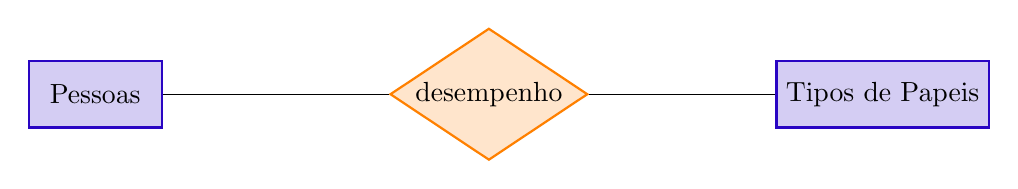
\begin{tikzpicture}
  [every entity/.style={fill=blue!20,draw=blue,thick},
   every relationship/.style={fill=orange!20,draw=orange,thick,aspect=1.5}]
  \node[entity] (Pessoas)  at (0,0)   {Pessoas};
  \node[entity] (TiposdePapeis) at (10,0)   {Tipos de Papeis};
  \node[relationship]    at (5,0) {desempenho}
    edge (Pessoas)
    edge (TiposdePapeis);
\end{tikzpicture}

Seguindo novamente  Setzer e Silva (2017), podemos interpretar a associa\c{c}\~ao \textquotedbl Desempenho\textquotedbl  da seguinte maneira: da esquerda para a direita a associa\c{c}\~ao significa que \textquotedbl Pessoas\textquotedbl  desempenham \textquotedbl Tipos de Papeis\textquotedbl  e, da direita para a esquerda, significa que \textquotedbl Tipos de Papeis\textquotedbl  s\~ao desempenhados por \textquotedbl Pessoas\textquotedbl .










Um problema desta forma de representa\c{c}\~ao da associa\c{c}\~ao desempenho, utilizando apenas duas entidades, \'e que n\~ao conseguimos identificar em que institui\c{c}\~ao o papel \'e desempenhado.










Vamos supor que a pessoa \textquotedbl Pedro\textquotedbl , enquanto era aluno do ensino m\'edio, desempenhou o papel de aluno da Escola Estadual Vitor Meirelles. Depois, quando entrou para o ensino superior, passou a desempenhar o papel de aluno junto \`a Universidade Estadual de Campinas. Essa situa\c{c}\~ao mostra que a associa\c{c}\~ao \textquotedbl Desempenho\textquotedbl  tem que ser tern\'aria, ou seja, tem que envolver as entidades \textquotedbl Pessoas\textquotedbl , \textquotedbl Tipos de Papeis\textquotedbl  e \textquotedbl Institui\c{c}\~oes\textquotedbl . Vimos na fundamenta\c{c}\~ao te\'orica como esse tipo de associa\c{c}\~ao \'e representada pela Fig. XXX.










Desta forma, h\'a que se usar uma representa\c{c}\~ao tern\'aria para representar \textquotedbl a que institui\c{c}\~ao a pessoa estava vinculada, quando desempenhou um determinado papel\textquotedbl , como segue. Na associa\c{c}\~ao tern\'aria, \'e comum usar a sigla formada pela primeira letra de cada entidade como nome da Associa\c{c}\~ao:











\begin{tikzpicture}
  [every entity/.style={fill=blue!20,draw=blue,thick},
   every relationship/.style={fill=orange!20,draw=orange,thick,aspect=1.5}]
  \node[entity] (Pessoas)  at (0,0)   {Pessoas};
  \node[entity] (TiposdePapeis) at (10,0)   {Tipos de Papeis};
  \node[entity] (Institui\c{c}\~oes) at (5,-3)   {Institui\c{c}\~oes};
  \node[relationship]    at (5,0) {P - TP - I}
    edge (Pessoas)
    edge (TiposdePapeis)
    edge (Institui\c{c}\~oes)
	;
\end{tikzpicture}

Feita a ressalva de que a associa\c{c}\~ao \textquotedbl P - TP - I\textquotedbl  tem que ser do tipo tern\'aria, ou seja, tem que relacionar 3 entidades, vamos dar um passo atr\'as na complexidade dessa representa\c{c}\~ao. Isso ser\'a feito para que possamos explicar a l\'ogica da representa\c{c}\~ao de uma associa\c{c}\~ao no conceito de teoria de conjuntos.










Portanto, apenas para efeito de exemplo, vamos considerar, temporariamente, que a rela\c{c}\~ao \textquotedbl Desempenho\textquotedbl  envolve apenas \textquotedbl Pessoas\textquotedbl  e \textquotedbl Tipos de Papeis\textquotedbl , desconsiderando que o desempenho do tipo de papel tem que estar vinculado a alguma institui\c{c}\~ao.










Com essa simplifica\c{c}\~ao, vamos dar alguns exemplos elucidativos.










Na tabela XXX apresentamos nomes de pessoas que fazem parte da entidade \textquotedbl Pessoas\textquotedbl .














\begin{table}[htb]
\tiny
\caption{\label{c8ffe3a57eead8658d31a50847a2f585edf5f62a}Exemplo de lista de pessoas pertencentes `a entidade Pessoas}

\centering
\begin{tabular}{|c|}
\hline
Entidade \textquotedbl Pessoas\textquotedbl  \\
Pedro \\
Jo\~ao \\
Maria \\
Roberta \\
M\'ario \\
\hline
\end{tabular}
\end{table}


Na tabela XXX apresentamos uma lista de papeis relativos \`a entidade \textquotedbl Tipos de Papeis\textquotedbl .














\begin{table}[htb]
\tiny
\caption{\label{8458b44ade0ed84477994a1c38837b638e3627b8}Exemplo de lista de tipos de papeis pertencentes `a entidade Tipos de Papeis}

\centering
\begin{tabular}{|c|}
\hline
Entidade \textquotedbl Tipos de Papeis\textquotedbl  \\
\hline
alunos \\
multiplicadores \\
servidores \\
cientistas \\
bolsistas \\
coordenadores \\
volunt\'arios \\
palestrantes \\
educando \\
\hline
\end{tabular}
\end{table}


Vamos tentar entender como \textquotedbl funciona\textquotedbl  a associa\c{c}\~ao \textquotedbl Desempenho\textquotedbl , no contexto do WASH, selecionando um dos elementos da entidade \textquotedbl Pessoas\textquotedbl  como exemplo.










Vamos escolher Pedro como exemplo e imaginar que ele, neste momento, \'e um aluno do ensino fundamental.










Considerando \textquotedbl Pedro\textquotedbl  como um elemento da entidade \textquotedbl Pessoas\textquotedbl  e \textquotedbl aluno do fundamental\textquotedbl  como um elemento da entidade \textquotedbl Tipos de Papeis\textquotedbl  (ver Fig. XXX), podemos ler a associa\c{c}\~ao \textquotedbl Desempenho\textquotedbl  da seguinte forma:











\noindent\begin{center}\mbox{\centering\fbox{\centering\par\parbox{0.7\linewidth}{\small\textit{\textquotedbl Pedro\textquotedbl  desempenha papel de \textquotedbl aluno do fundamental\textquotedbl }\normalsize}}}\end{center}


No sentido inverso a associa\c{c}\~ao \textquotedbl Desempenho\textquotedbl  nos remete a:











\noindent\begin{center}\mbox{\centering\fbox{\centering\par\parbox{0.7\linewidth}{\small\textit{\textquotedbl aluno do fundamental\textquotedbl  \'e papel desempenhado por \textquotedbl Pedro\textquotedbl }\normalsize}}}\end{center}




\captionsetup{format=plain}
\begin{figure}[htb]

	\begin{center}

		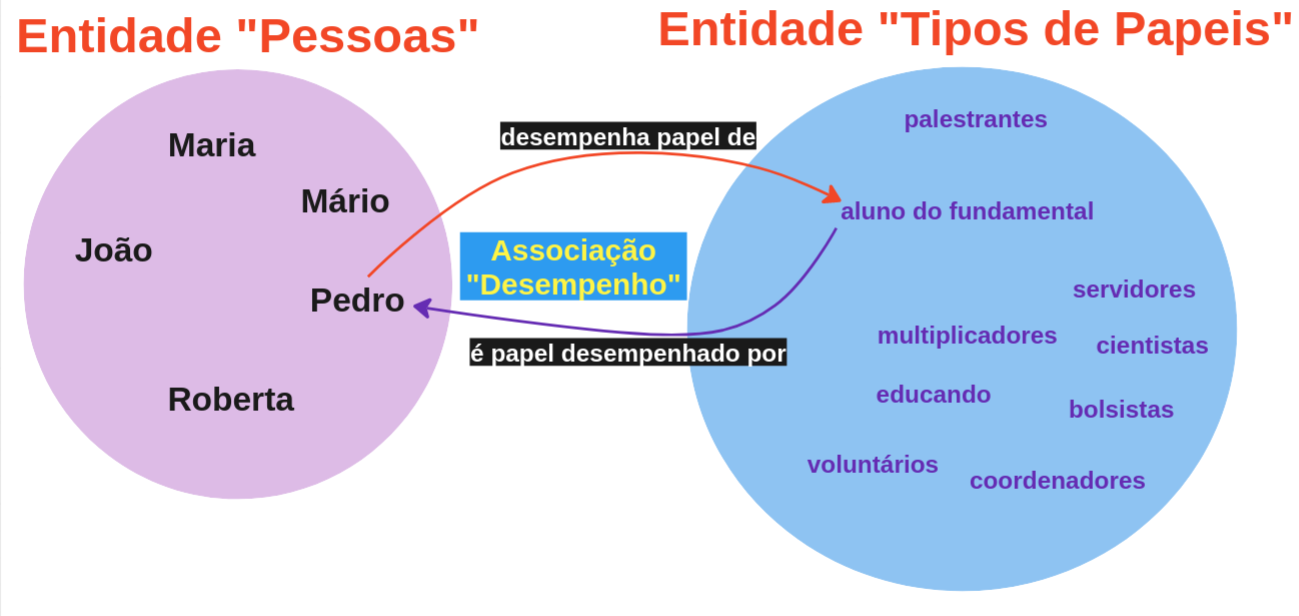
\includegraphics[max size={\textwidth}{\textheight}]{../../imagens/DiagramaVenn.png}

	\end{center}

	\caption{\label{7e3f7eeaec97530625b5f966674efc609d307ae6}Diagrama de Venn representando duas entidades (Pessoas e Tipos de Papeis) e uma associa\c{c}\~ao (Desempenho).}

\end{figure}

Mas a associa\c{c}\~ao \textquotedbl desempenho\textquotedbl  deve permitir que Pedro assuma nenhum, um ou mais de um papel, concomitantes, simult\^aneos ou parcialmente sobrepostos. Para que a temporalidade dos papeis desempenhados possa ser representada, \'e preciso indicar a data de in\'{\i}cio e de fim para aquele papel.










Vamos criar uma situa\c{c}\~ao hip\'otetica de pap\'eis simult\^aneos para Pedro. Para o exemplo ficar mais claro, acompanhe na figura XXX, que busca representar a associa\c{c}\~ao \textquotedbl Desempenho\textquotedbl  na forma de uma linha de tempo.










A figura XXX mostra um elemento da entidade \textquotedbl Pessoas\textquotedbl , no caso \textquotedbl Pedro\textquotedbl , representado pela seta azul. A figura tamb\'em mostra seis elementos da Entidade \textquotedbl Tipos de Papeis\textquotedbl , representados pelas setas vermelhas.










A seta (1) da Fig XXX indica que Pedro desempenhou o papel de \textquotedbl aluno do fundamental\textquotedbl  por um certo per\'{\i}odo. A seta (2) indica que, um pouco depois de iniciar suas atividades como \textquotedbl aluno do fundamental\textquotedbl , ele passou a frequentar as oficinas do WASH, desempenhando o papel de \textquotedbl Participante do WASH\textquotedbl . Vemos que o papel indicado pela seta (1) chegou ao fim, substitu\'{\i}do pelo papel indicado pela seta (3), que \'e o de \textquotedbl aluno do ensino m\'edio\textquotedbl . Simultaneamente ao papel de \textquotedbl aluno do ensino m\'edio\textquotedbl , Pedro foi convidado pela equipe do WASH para assumir o papel de \textquotedbl multiplicador\textquotedbl  do WASH, como indica a seta (4). Como Pedro n\~ao tinha bolsa na fase inicial do papel \textquotedbl multiplicador\textquotedbl , naquele per\'{\i}odo ele estava desempenhando o papel de \textquotedbl volunt\'ario\textquotedbl , como indicado pela seta (5). A partir do in\'{\i}cio da seta (6), quando a equipe ofereceu uma bolsa, ele passou a ser \textquotedbl bolsista\textquotedbl  e a seta (5) teve que ser finalizada.












\captionsetup{format=plain}
\begin{figure}[htb]

	\begin{center}

		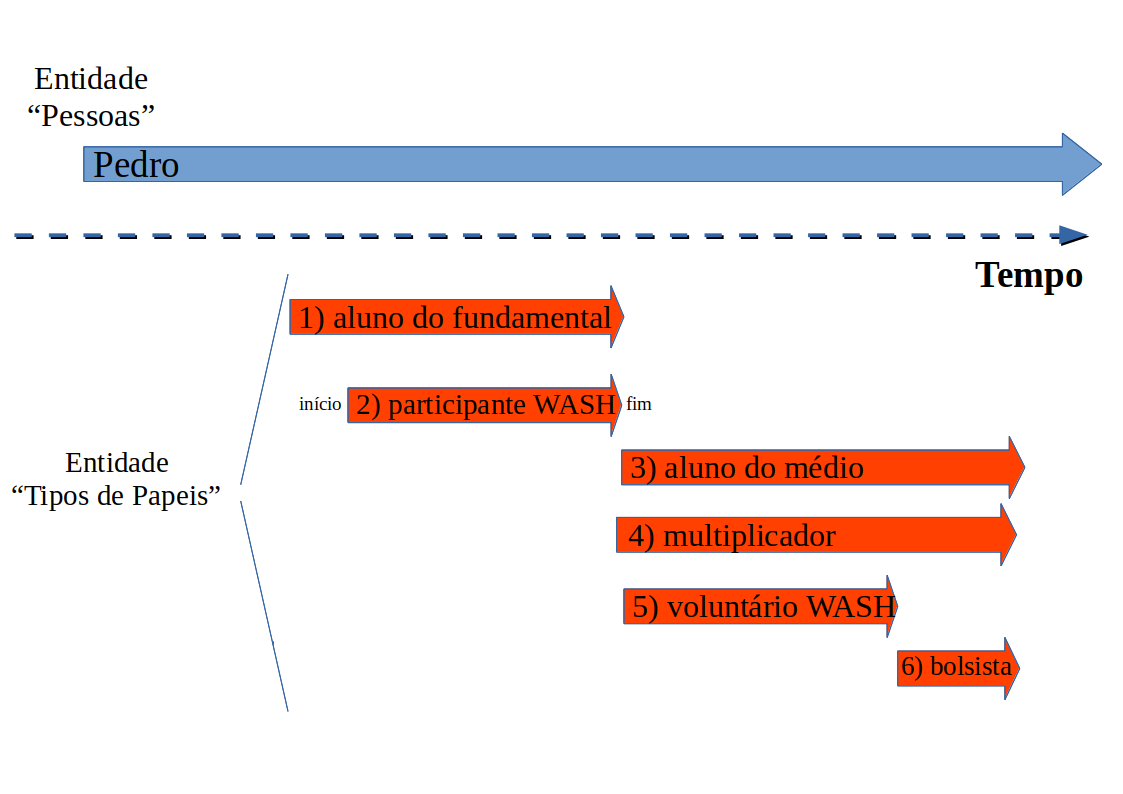
\includegraphics[max size={\textwidth}{\textheight}]{../../imagens/digrama-associacoes4.png}

	\end{center}

	\caption{\label{14807bc5605d321570600aeb32f379a2d4eba9f9}A associa\c{c}\~ao Desempenho representada como linha do tempo.}

\end{figure}

 Portanto, a associa\c{c}\~ao \textquotedbl desempenho\textquotedbl  deve contemplar a possibilidade de Pedro ter um ou mais papeis, com a possibilidade de sobreposi\c{c}\~ao temporal, seja integral ou parcial.










Considerando a associa\c{c}\~ao \textquotedbl desempenho\textquotedbl  no sentido oposto, esta deve contemplar a possibilidade de um determinado tipo de papel ser desempenhado por mais de uma pessoa. Por exemplo, o tipo de papel \textquotedbl participante\textquotedbl  deve ser pass\'{\i}vel de ser desempenhado por milhares de participantes do WASH. O papel \textquotedbl coordenador\textquotedbl  deve ser pass\'{\i}vel de ser desempenhado por muitos participantes do WASH, dado que existem coordena\c{c}\~oes locais no programa.










Esta forma bi-direcional de analisar a associa\c{c}\~ao \textquotedbl desempenho\textquotedbl  ajuda, posteriormente, a equipe de TI definir a \textquotedbl cardinalidade\textquotedbl  (ou multiplicidade) das rela\c{c}\~oes no Modelo Conceitual de Entidade-Relacionamento.










Como estamos no n\'{\i}vel de abstra\c{c}\~ao descritivo, n\~ao aprofundaremos na quest\~ao da cardinalidade dos relacionamentos, permanecendo numa descri\c{c}\~ao por meio de linguagem natural das associa\c{c}\~oes encontradas no WASH. Esta descri\c{c}\~ao da cardinalidade, usando linguagem natural, estar\'a presente no cap\'{\i}tulo de Resultados e An\'alise.










O m\'etodo de infer\^encia aqui descrito foi aplicado repetidamente, visando identificar as entidades e associa\c{c}\~oes mais relevantes para a modelagem do Programa WASH.










A lista completa de entidades e associa\c{c}\~oes encontradas para o Programa WASH pela aplica\c{c}\~ao deste m\'etodo est\'a no cap\'{\i}tulo de Resultados e An\'alise.










\subsection[Como modelar os processos de neg\'ocio (BPMN)]{Como modelar os processos de neg\'ocio (BPMN)}\label{Como modelar os processos de neg\'ocio (BPMN)}
primeiro










\section[Caminho para a obten\c{c}\~ao dos indicadores (eixo 3)]{Caminho para a obten\c{c}\~ao dos indicadores (eixo 3)}\label{Caminho para a obten\c{c}\~ao dos indicadores (eixo 3)}
\subsection[M\'etodo de Estrutura\c{c}\~ao e an\'alise dos dados]{M\'etodo de Estrutura\c{c}\~ao e an\'alise dos dados}\label{M\'etodo de Estrutura\c{c}\~ao e an\'alise dos dados}
Vimos no cap\'{\i}tulo de Fundamenta\c{c}\~ao Te\'orica que os Bancos de Dados Relacionais oferecem uma melhor forma de representar dados complexos como os do WASH em rela\c{c}\~ao ao uso de planilhas eletr\^onicas ou outras formas menos estruturadas.










A compara\c{c}\~ao que fizemos com planilhas eletr\^onicas mostrou que estas ferramentas, ao contr\'ario do modelo relacional, s\~ao mais propensas aos erros de digita\c{c}\~ao, falta de uniformiza\c{c}\~ao no preenchimento de dados, falta de seguran\c{c}a e prote\c{c}\~ao da informa\c{c}\~ao, dentre outras desvantagens.










A escolha do modelo relacional para representar os dados do WASH, em substitui\c{c}\~ao \`as planilhas eletr\^onicas, foi proposta pelo coordenador do Projeto, Victor Pellegrini Mammana, que passou a promover di\'alogos para identificar a melhor forma de representar os dados.










Para implementar o modelo em um software-aplicativo, foi escolhida uma plataforma baseada nos seguintes softwares:











\begin{alineas}
\item Sistema Operacional do servidor: LINUX
\item Servidor de p\'aginas WEB: Apache
\item Servidor de Banco de Dados: MySQL
\item Linguagens de Programa\c{c}\~ao: PHP, Javascript e SQL
\end{alineas}

Os detalhes de implementa\c{c}\~ao dessas plataformas fogem ao escopo de forma\c{c}\~ao desta candidata, raz\~ao pela qual nesta parte do trabalho nos concentraremos apenas na caracteriza\c{c}\~ao do modelo de banco de dados relacional que foi implementado no servidor MySQL.










Este software-aplicativo foi denominado \textquotedbl Platu\'osh\textquotedbl  e contou com a participa\c{c}\~ao da presente candidata em sua concep\c{c}\~ao  (MAMMANA et al., 2022).










A contribui\c{c}\~ao para a concep\c{c}\~ao do software concentrou-se nos primeiros exerc\'{\i}cios de registro de presen\c{c}a e de realiza\c{c}\~ao de oficinas, realizado por n\'os utilizando meios f\'{\i}sicos. Propusemos um sistema de testemunhos documentais para comprovar a realiza\c{c}\~ao das oficinas, colecionando notas em Di\'arios de Bordo, fotografias, listas de presen\c{c}a e material de divulga\c{c}\~ao das oficinas.












\captionsetup{format=plain}
\begin{figure}[max size={\textwidth}{\textheight}]

\centering


\begin{minipage}[b]{0.4\linewidth}
        \centering
                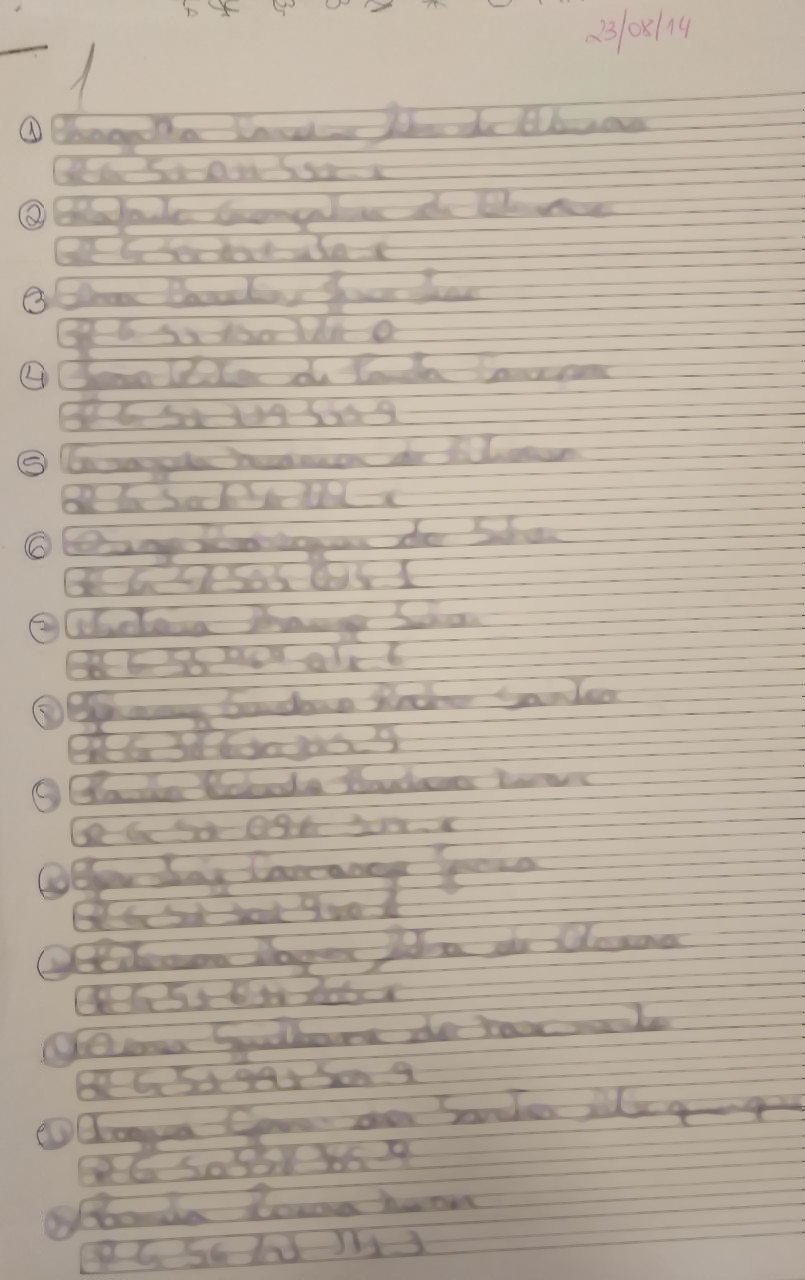
\includegraphics[width=1.0\linewidth]{../../imagens/blurred-Presenca-Oficina-2014-08-23.jpeg}
                \caption{Testemunhos de presen\c{c}a de estudantes do fundamental em eventos do Programa WASH coletados pela candidata. O exemplo \'e de uma oficina em 23 de agosto de 2014. Nos prim\'ordios do projeto eram usados registros na forma de listas de presen\c{c}a em folhas de papel. A imagem foi desfocalizada para proteger a privacidade dos participantes.}
                \label{dec219c809788f521312f8d75d2f5591f069f132}
\end{minipage}%
\hspace{0.5cm}
\begin{minipage}[b]{0.4\linewidth}
        \centering
                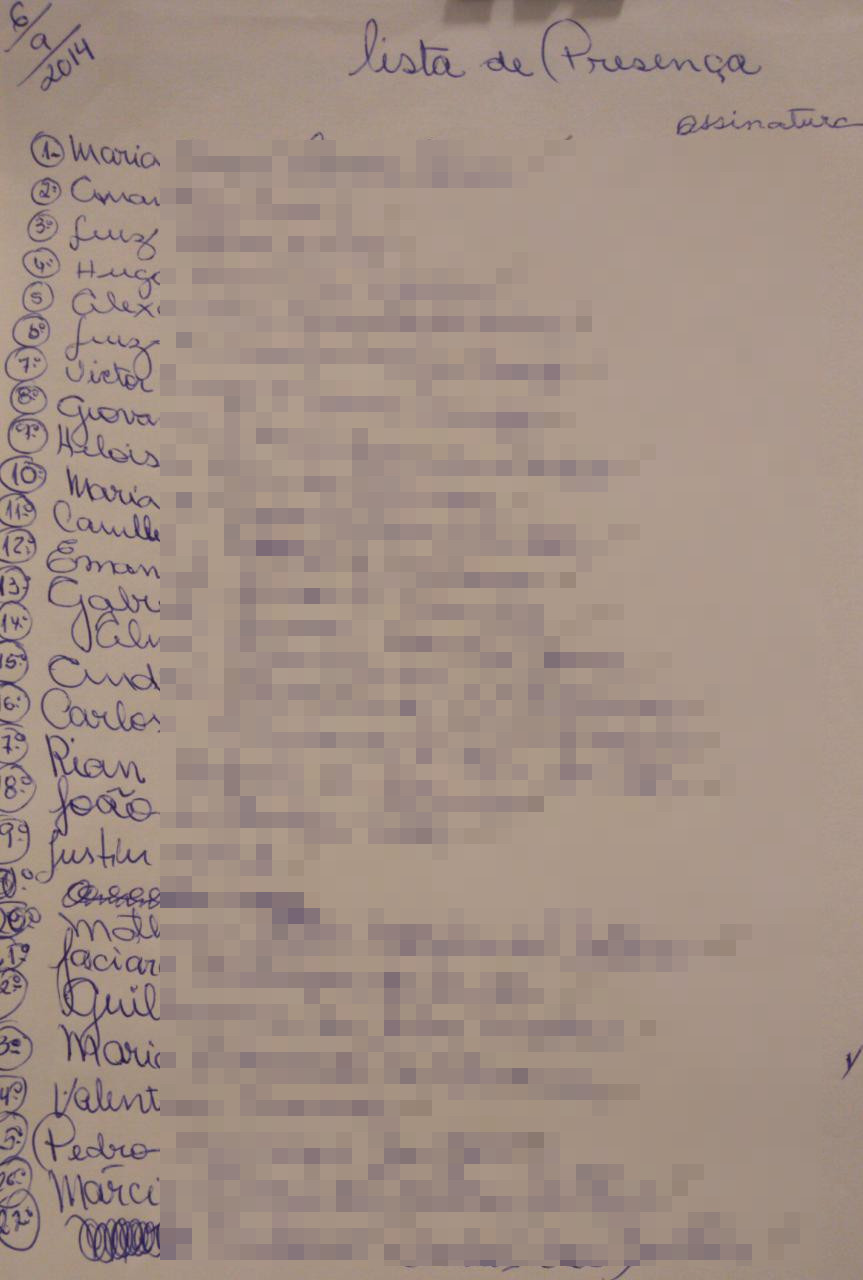
\includegraphics[width=1.0\linewidth]{../../imagens/blurred-Presenca-Oficina-2014-09-06.jpeg}
                \caption{Exemplo de lista de presen\c{c}a em papel, da oficina realizada em 6 de setembro de 2014. A imagem foi desfocalizada para proteger a privacidade dos participantes. Estes testemunhos eram coletados pela candidata para permitir a posterior presta\c{c}\~ao de contas aos \'org\~aos de fomento.}
                \label{9a8c04c719fc4f9811165547ded35a00eb4fbeed}
\end{minipage}
\hspace{0.5cm}
\begin{minipage}[b]{0.4\linewidth}
        \centering
                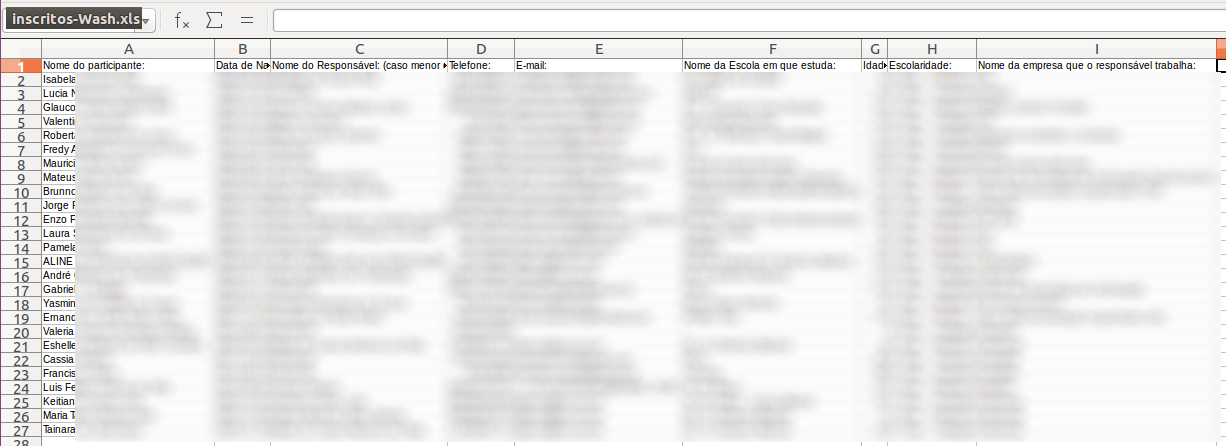
\includegraphics[width=1.0\linewidth]{../../imagens/blurred-planilha2.png}
                \caption{Planilhas eletr\^onicas tamb\'em foram empregadas para armazenar os registros de participa\c{c}\~oes, criando um proto-cadastro de participantes. A imagem foi desfocalizada intencionalmente para proteger a privacidade dos participantes.}
                \label{b43907f0fa6b6fb935e7384ab03b508859ff0609}
\end{minipage}%
\hspace{0.5cm}
\end{figure}



Logo ficou evidente que o crescimento do Programa WASH exigiria um m\'etodo mais eficiente de armazenagem dos testemunhos de participa\c{c}\~ao, que permitisse tamb\'em individualizar a identidade dos participantes.










A import\^ancia de individualizar as presen\c{c}as come\c{c}ou a ficar evidente quando se percebeu que o WASH tinha uma alta rotatividade de participantes, mas que tamb\'em mantinha uma parcela fiel de \textquotedbl p\'ublico\textquotedbl . Portanto era preciso saber quando um participante voltava e isso s\'o era poss\'{\i}vel individualizando seu registro. Inicialmente foi usado o nome do participante, o nome do respons\'avel e a data de nascimento, como forma de identificar univocamente um participante.










Esse cuidado em individualizar os participantes permitia, por exemplo, ter uma melhor no\c{c}\~ao do perfil et\'ario do p\'ublico atendido, bem como do interesse em participar novamente das atividades, entre tantos outros indicadores que ficar\~ao mais claros no cap\'{\i}tulo de Resultados e An\'alise. Outro aspecto favor\'avel da individualiza\c{c}\~ao era uma melhor organiza\c{c}\~ao dos documentos do projeto, tais como autoriza\c{c}\~oes para a participa\c{c}\~ao de menores, consentimento de uso de imagem, identifica\c{c}\~ao de respons\'aveis para casos de emerg\^encia, entre outros.










A partir deste esfor\c{c}o inicial de coleta e organiza\c{c}\~ao de testemunhos de oficinas realizado pela candidata, foi elaborada uma primeira vers\~ao do Platu\'osh, que permitia registrar as oficinas realizadas, os participantes nominalmente e os testemunhos de realiza\c{c}\~ao. Essa primeira vers\~ao do software, que ficou pronta no in\'{\i}cio de 2019, passou a ser usada para gerar os indicadores do projeto, de forma rastre\'avel, provendo meios confi\'aveis de prestar contas aos \'org\~aos de fomento e de controle.










A Platu\'osh foi sendo evolu\'{\i}da paulatinamente a partir do teste constante de suas funcionalidades, atividade da qual participamos intensamente, juntamente com outros membros do projeto. A cada teste eram identificados os problemas, com a subsequente propostas de alternativas, que eram implementadas pela equipe respons\'avel pela codifica\c{c}\~ao do programa.










Uma atividade fundamental conduzida pela equipe de codifica\c{c}\~ao foi a modelagem de dados, visando estabelecer quais tabelas seriam necess\'arias para representar os dados do WASH. Esta modelagem tinha como base as informa\c{c}\~oes fornecidas pelos participantes do WASH envolvidos com sua opera\c{c}\~ao na ponta, equipe que era coordenada por n\'os.










A Platu\'osh foi desenvolvida diretamente a partir do Modelo de Dados Relacional (MDR), sem passar pela etapa intermedi\'aria da Modelagem Entidade Relacionamento. Isso gerou uma s\'erie de defici\^encias no MDR da Platu\'osh, que ser\~ao discutidas posteriormente. Essas defici\^encias ficar\~ao mais evidentes quando o MDR da Platu\'osh for comparada com o Modelo H\'{\i}brido desenvolvido no \^ambito desta disserta\c{c}\~ao.










Para identificar o n\'umero de tabelas que seria necess\'ario foram feitas v\'arias considera\c{c}\~oes, a partir da contribui\c{c}\~ao de v\'arios membros do projeto. Infelizmente, a equipe de TI do WASH optou por n\~ao realizar um modelo MER anteriormente \`a modelagem MDR. Alguns defici\^encias decorrentes dessa escolha podem ser identificadas no modelo de dados do Programa.










Como j\'a dito, uma das quest\~oes centrais no registro de dados do Programa WASH \'e saber quem s\~ao os seus participantes. No come\c{c}o da modelagem dos dados, havia uma d\'uvida sobre se dever\'{\i}amos criar uma tabela para alunos benefici\'arios (principalmente ensino fundamental), outra para os membros da equipe do WASH e mais outra para os bolsistas multiplicadores. Uma outra op\c{c}\~ao seria criar tabela \'unica para todos os participantes, independentemente de seu papel no projeto. No caso de se optar pela cria\c{c}\~ao de uma tabela \'unica, seria necess\'ario uma tabela auxiliar, que contivesse os \textquotedbl tipos de papeis\textquotedbl  pass\'{\i}veis de serem desempenhados por um participante.










A segunda op\c{c}\~ao foi a escolhida porque j\'a se antecipava que o WASH seria um projeto de longo prazo. Quando o sistema de registro come\c{c}ou a ser elaborado, o WASH j\'a tinha 6 anos e o crescimento anual indicava que haveria f\^olego para muitos anos mais de execu\c{c}\~ao. Assim, n\~ao fazia sentido separar os participantes em diversas tabelas, porque era razo\'avel esperar a mudan\c{c}a de papeis dos participantes, situa\c{c}\~ao que j\'a era observada em alguns casos.










De fato, observava-se que alunos do ensino fundamental, ao adentrar no ensino m\'edio, passavam a receber bolsas de inicia\c{c}\~ao cient\'{\i}fica, tornando-se bolsistas multiplicadores. Bolsistas multplicadores do ensino superior, ao se formarem em seus cursos, passavam a ser membros da equipe do WASH. Muitos casos de transi\c{c}\~ao de papeis puderam ser constatados e a ideia de ter m\'ultiplas tabelas para participantes implicaria em um complicado sistema de transi\c{c}\~ao do registro de uma tabela para outra, quando o participante mudasse de papel. Outro motivo para usar a tabela \'unica \'e que j\'a se observavam casos de papeis simult\^aneos, a exemplo de multiplicadores que tamb\'em eram servidores p\'ublicos.










Assim, decidiu-se por criar uma tabela \'unica de participantes que foi denominada \textquotedbl participantes2\textquotedbl , que est\'a em uso at\'e os dias de hoje. Esta tabela \'e complementada por duas outras: \textquotedbl cargos\textquotedbl , que cont\'em os tipos de vincula\c{c}\~ao com o WASH e \textquotedbl institui\c{c}\~oes\textquotedbl , que cont\'em as institui\c{c}\~oes a que um participante pode estar vinculado. Para ligar o participante a um cargo e a uma institui\c{c}\~ao, foi criada a tabela \textquotedbl afiliacoes\textquotedbl , que cont\'em o data de in\'{\i}cio e a data do fim daquela afialia\c{c}\~ao.










Este conjunto de tabelas exemplifica a l\'ogica da modelagem que foi constru\'{\i}da para representar os dados do WASH e come\c{c}aremos mostrando o conte\'udo (parcial) da tabela de \textquotedbl cargos\textquotedbl :














\begin{table}[htb]
\tiny
\caption{\label{8da11be906e8c6597b09624b6ea24ac1ac2e1607}Vis\~ao parcial da tabela cargos da base de dados do WASH. A tabela completa tem 42 linhas com registros de cargos.}

\centering
\begin{tabular}{|c|c|}
\hline
id\_chave\_cargo  &  nome\_cargo            \\
             9  &  Coordenador           \\
            10  &  Bolsista EXP A        \\
            11  &  Educando              \\
            13  &  Professor             \\
            15  &  Presidente            \\
            16  &  Diretor               \\
            17  &  Servidor              \\
            18  &  Coordenador Local     \\
            19  &  Coordenador Nacional  \\
            21  &  Deputado              \\
            22  &  Presidente            \\
            23  &  Multiplicador         \\
            25  &  Bolsista PCI   \\
            26  &  Bolsista ITI A \\
            27  &  Bolsista ITI B \\
            28  &  Reitor \\
            31  &  Secretaria \\
            38  &  Prefeito              \\
            39  &  Pesquisador           \\
            40  &  Secretaria Executiva  \\
            41  &  Voluntario            \\
            42  &  Estudante    \\
            43  &  Estagiario \\
            48  &  Bolsista EXP B \\
            49  &  Bolsista EXP C \\
            50  &  Bolsista ATP B \\
            51  &  Educando \\
            52  &  Voluntario \\
            54  &  Orientador            \\
            55  &  Bolsista DTI A \\
\hline
\end{tabular}
\end{table}


Na sequ\^encia mostramos uma vis\~ao parcial da tabela \textquotedbl Instituicoes\textquotedbl , que cont\'em todas as institui\c{c}\~oes atendidas pelo WASH. A tabela completa tem 150 linhas de registros de institui\c{c}\~oes, mas estamos mostrando apenas 38 por motivos de espa\c{c}o.














\begin{table}[htb]
\tiny
\caption{\label{c00aa31debbd8e46e29d5e4041d1141591dbe97d}Vis\~ao parcial da tabela instituicoes da base de dados do WASH. A tabela completa tem 150 linhas com registros de institui\c{c}\~oes. Na presente reprodu\c{c}\~ao foram selecionados registros que mostram a pluralidade do atendimento do WASH, tendo sido retirados as repeti\c{c}\~oes de tipos de institui\c{c}\~oes por motivos de espa\c{c}o.}

\centering
\begin{tabular}{|c|c|}
\hline
id\_chave\_instituicao  &  nome\_instituicao \\
                  164  &  APAE  \\
                   68  &  Associa\c{c}\~ao Cultural Bola de Meia \\
                   74  &  Biblioteca Cidad\~a Paulo Freire  \\
                   52  &  Camara Federal \\
                   32  &  C\^amara Municipal de Campinas                                                      \\
                   25  &  Casa de Cultura Taina                                                             \\
                  168  &  CEI Vov\'o Maria                                                                    \\
                   23  &  Cemaden                                                                           \\
                  150  &  Centro de Forma\c{c}\~ao Popular Frei Betto                                             \\
                   19  &  Centro Paula Souza                                                                \\
                   22  &  Ci\^encia em Show                                                                   \\
                   57  &  CNPq                                                                              \\
                   91  &  Col\'egio Estadual Rio Branco                                                       \\
                   56  &  CPqD                                                                              \\
                    1  &  CTI Renato Archer                                                                 \\
                   70  &  E.E. Vitor Meireles                                                               \\
                   80  &  E.E. Expedito Camargo Freire                                                      \\
                  130  &  EMEF D\'ecio Moreira \\
                    5  &  Escola Dona Lindu \\
                  128  &  Escola Estadual MAJOR MIGUEL NAKED \\
                  111  &  ETEC Carapicu\'{\i}ba \\
                   47  &  Ex\'ercito Brasileiro \\
                  156  &  Faculdade Zumbi dos Palmares \\
                   53  &  FAPESP \\
                  119  &  Funda\c{c}\~ao Arauc\'aria \\
                   35  &  Governo do Estado de S\~ao Paulo \\
                  127  &  IFPR - Campus Pitanga \\
                   62  &  PUC de Campinas \\
                   21  &  Prefeitura de S\~ao Paulo           \\
                   48  &  Secreataria de Cultura de Londrina \\
                   49  &  Secretaria de Cultura de Londrina \\
                   85  &  Secretaria de Educa\c{c}\~ao de Jacare\'{\i}/SP \\
                  169  &  SENAC Minas  \\
                   38  &  Sindicato dos Metal\'urgicos do ABC \\
                   16  &  Unicamp \\
                   75  &  UNIFESP  \\
                    9  &  USP \\
                  181  &  UTFPR \\
\hline
\end{tabular}
\end{table}


Para dar prosseguimento \`a exemplifica\c{c}\~ao, agora selecionaremos um participante do projeto para extrair seu registro da tabela \textquotedbl participantes2\textquotedbl . Note que esta tabela tem 3312 registros mas decidimos usar como exemplo um \'unico participante, isolando a linha da tabela que se refere a este participante. Retiramos, tamb\'em, todos os dados pessoais do participante, para proteger sua privacidade, substituindo seu nome por \textquotedbl Nome de Participante omitido\textquotedbl :














\begin{table}[htb]
\tiny
\caption{\label{2c8d9dda4031f0ea459292d025586b4d3e57ed84}Exemplo de linha da tabela participantes2, selecionada para que se possa entender como o registro dos papeis desempenhados por cada participante \'e feito no \^ambito do WASH. A tabela participantes2 tem 3312 registros de participantes.}

\centering
\begin{tabular}{|c|c|c|}
\hline
id\_chave\_participante  &  nome\_participante             &  data\_nascimento  \\
                     2  &  Nome de Participante omitido  &  1994-06-15 \\
\hline
\end{tabular}
\end{table}


\'E importante notar que, por escolha da \'area de TI do projeto, todas as datas no \^ambito dos registros do Programa WASH s\~ao invertidas, sempre come\c{c}ando pelo ano, passando pelo m\^es e terminando no dia. Isto \'e feito assim para garantir que a ordena\c{c}\~ao dos registros por data seja facilitada.










Agora vamos extrair da tabela \textquotedbl afiliacoes\textquotedbl  todos os registros cujo identificador de participante seja \textquotedbl 2\textquotedbl , como consta na tabela participantes2:














\begin{table}[htb]
\tiny
\caption{\label{e6120545268b93238330297571c4756e7c97df1a}Subconjunto de registro da tabela afiliacoes, onde foram selecionados apenas os dados do participante que tem identificador 2 na tabela participantes2.}

\centering
\begin{tabular}{|c|c|c|c|c|c|}
\hline
id\_participante  &  id\_instituicao  &  id\_cargo  &  nome\_documento  &  inicio      &  fim \\
              2  &              62  &        42  &  RA12345679      &  2012-02-01  &  2015-01-31  \\
              2  &              57  &        48  &  111111/2018-9   &  2018-08-01  &  2019-07-31  \\
              2  &              57  &        48  &  222222/2019-6   &  2019-08-01  &  2019-12-31  \\
              2  &              57  &        48  &  333333/2019-2   &  2020-08-01  &  2021-12-31  \\
              2  &              57  &        26  &  444444/2016-1   &  2016-08-02  &  2017-07-31  \\
              2  &              62  &        52  &  n\~ao consta      &  2015-08-01  &  2016-08-01 \\
\hline
\end{tabular}
\end{table}


O excerto da tabela \textquotedbl afiliacoes\textquotedbl  mostrado indica que o participante identificado pelo n\'umero 2 teve 2 afilia\c{c}\~oes durante o per\'{\i}odo em que esteve vinculado ao WASH: \`a universidade PUC de Campinas, que \'e identificada pelo n\'umero 62 e ao CNPq, que \'e identificado pelo n\'umero 57.










Al\'em disso, esse mesmo participante identificado pelo n\'umero 2 desempenhou 4 papeis no \^ambito do WASH: estudante, identificado pelo n\'umero 42, Bolsista EXP B, identificado pelo n\'umero 48 e Bolsista ITI A, identificado pelo n\'umero 26.










A tabela \textquotedbl afiliacoes\textquotedbl  tamb\'em permite conhecer o documento que formaliza a vincula\c{c}\~ao com o Programa WASH, pelo campo nome\_documento. Os campos \textquotedbl inicio\textquotedbl  e \textquotedbl fim\textquotedbl  permitem conhecer o per\'{\i}odo em que uma determinada afilia\c{c}\~ao estava v\'alida.










O exemplo mostrado at\'e agora permite compreender como funcionam os bancos de dados relacionais de uma forma pr\'atica, usando o caso do WASH como exemplo.










O sistema de armazenamento de dados do WASH \'e integralmente baseado nessa l\'ogica de m\'ultiplas tabelas que se relacionam por meio de identificadores n\'umericos. Esse m\'etodo \'e bastante robusto e reduz sobremaneira a ocorr\^encia de dados esp\'urios, muito embora ainda exista a possibilidade de algum erro estar presente, porque a integridade da base de dado \'e dependente da qualidade do preenchimento de dados. Isso quer dizer que, para garantir a qualidade de dados, \'e preciso uma capacita\c{c}\~ao constante dos colaboradores.










A maior robustez do m\'etodo relacional vem justamente do fato de que a informa\c{c}\~ao est\'a segregada, de forma que em cada tabela exista apenas um registro para cada fato representado. Em outras palavras: note que na tabela \textquotedbl participantes2\textquotedbl  existir\'a apenas 1 registro para o participante que \'e identificado pelo n\'umero 2, ao passo que na tabela \textquotedbl cargos\textquotedbl  haver\'a apenas um registro identificado pelo n\'umero 48 (Bolsista EXP B), da mesma forma que na tabela \textquotedbl instituicoes\textquotedbl  haver\'a apenas um registro identificado pela n\'umero 57 (CNPq) e isso \'e verdade n\~ao importa quantas bolsas diferentes o participante identificado pelo n\'umero 2 tiver.










Vimos que o participante identificado pelo n\'umero \textquotedbl 2\textquotedbl  teve  pelo menos 6 diferentes tipos de v\'{\i}nculos com o WASH, em momentos diferentes de sua atua\c{c}\~ao, mas n\~ao foi preciso criar 6 registros na tabela \textquotedbl participantes2\textquotedbl . Se o WASH usasse planilhas eletr\^onicas para guardar seus dados seria necess\'ario repetir 6 vezes todas as informa\c{c}\~oes sobre o partipante, criando a oportunidade para falta de uniformiza\c{c}\~ao de dados e, portanto, perda de confiabilidade nos mesmos.










Para representar todos os seus dados de forma flex\'{\i}vel e adapt\'avel \`as suas diversas parcerias, o sistema de armazenamento de dados do WASH precisou criar 54 tabelas, que s\~ao mostradas a seguir:














\begin{table}[htb]
\tiny
\caption{\label{5b2e4ba8f3836249e7dd88b37344da7bfa3669c5}O bando de dados relacional subjacente `a Plataforma de Gest\~ao do WASH \'e constitu\'{i}do por 54 tabelas (P.S.: uma revis\~ao recente do modelo levou a 65 tabelas).}

\centering
\begin{tabular}{|c|c|}
\hline
afiliacoes                     &   local\_eventos \\
 atividades                     &   local\_part \\
 atividades\_eventos             &   modelo\_atividades\_eventos \\
 atividades\_fotos               &   modelo\_documentos\_eventos \\
 avaliacao\_bolsista             &   modelo\_eventos \\
 bolsa\_cnpq                     &   modelo\_tematicas\_eventos \\
 cargos                         &   parametros \\
 comentario\_evento              &   part\_eventos \\
 compartilhados                 &   participantes2 \\
 documentos                     &   processo\_cnpq \\
 documentos\_equipes             &   processo\_ivan\_valente \\
 documentos\_eventos             &   processo\_wash\_ABC \\
 documentos\_instituicoes        &   processo\_wash\_cury \\
 documentos\_participantes       &   processo\_wash\_regioes \\
 estimativa                     &   relacao\_grupo\_modelo \\
 eventos                        &   responsaveis\_eventos \\
 fontes                         &   status \\
 fontes\_eventos                 &   status\_doc \\
 formacao                       &   tematicas \\
 fotos                          &   tematicas\_eventos \\
 grupo\_evento                   &   tipo\_documento \\
 grupo\_modelo                   &   tipos\_encerramento \\
 grupo\_participante             &   trash \\
 grupos                         &   trash\_fontes \\
 inst\_eventos                   &   trash\_fotos \\
 instituicoes                   &   vincula\_instituicao\_instituicao \\
 locais                         &   vincula\_local\_instituicao \\
\hline
\end{tabular}
\end{table}


N\~ao aprofundaremos mais na descri\c{c}\~ao da modelagem de dados do Platu\'osh por raz\~oes de espa\c{c}o, mas acreditamos que as informa\c{c}\~oes at\'e agora compartilhadas permitem ao leitor compreender o m\'etodo de registro de dados utilizado.










\subsection[M\'etodo de determina\c{c}\~ao do sexo dos participantes]{M\'etodo de determina\c{c}\~ao do sexo dos participantes}\label{M\'etodo de determina\c{c}\~ao do sexo dos participantes}
A quest\~ao de armazenagem de dados de g\^enero no WASH ainda n\~ao est\'a devidamente equacionada e esta situa\c{c}\~ao tem a ver com a forma como os dados eram armazenados no in\'{\i}cio do projeto, assunto que passa a ser tratado a seguir.










\'E poss\'{\i}vel identificar v\'arios momentos na forma como o WASH armazenou seus dados ao longo de 9 anos. Como j\'a comentando na se\c{c}\~ao anterior, logo no in\'{\i}cio do projeto, os dados de participantes eram coletados por meio de listas de presen\c{c}a em papel, nas quais constavam inicialmente apenas o nome dos participantes e a data do evento. Posteriormente novos dados foram sendo coletados, como o ano do nascimento da crian\c{c}a, seu Registro Geral (RG) ou do respons\'avel.










Esse \textquotedbl crescendo\textquotedbl  na quantidade de dados coletados revela, por parte da coordena\c{c}\~ao do WASH, uma vis\~ao inicial minimalista no sentido dos dados que deveriam ser coletados. Essa forma de coletar dados pode ser atribu\'{\i}da ao fato do projeto ocorrer no contexto do servi\c{c}o p\'ublico, sem um mandato espec\'{\i}fico para registro de dados cadastrais mais detalhados.










Assim, \'e poss\'{\i}vel compreender porque a coleta de dados sempre foi mantida no limite dos prop\'ositos do projeto, a saber: contabilizar o n\'umero de participantes, evitar a contagem duplicada de participantes, identificar os respons\'aveis, registrar autoriza\c{c}\~oes de uso de imagens, etc., prop\'ositos estes j\'a bastante mencionados at\'e este ponto.










Consequentemente, por falta de prop\'osito, desde o in\'{\i}cio do projeto n\~ao havia a armazenagem do sexo de seus participantes.










Com o crescimento do projeto, come\c{c}ou a existir uma preocupa\c{c}\~ao sobre se o projeto era inclusivo, em termos de atendimento equ\^anime dos v\'arios perfis de g\^enero. Mas no momento em que essa defici\^encia de registro foi diagnosticada, o projeto j\'a contava com milhares de participa\c{c}\~oes. Isso exigiu a ado\c{c}\~ao de algum m\'etodo para tentar verificar se o atendimento era suficientemente equ\^anime, mesmo sem existirem registros cadastrais que indicassem o g\^enero dos participantes.










Criou-se um m\'etodo em que os indicadores de g\^enero do WASH s\~ao constru\'{\i}dos a partir de uma avalia\c{c}\~ao a posteriori dos primeiros nomes dos participantes, que s\~ao comparados com listas de nomes masculinos e de nomes femininos. Evidente que esta abordagem \'e imperfeita pela pr\'opria imprecis\~ao do conceito de \textquotedbl nomes masculinos\textquotedbl  e \textquotedbl nomes femininos\textquotedbl .










Avaliar a posteriore era necess\'ario porque para muitos registros, principalmente para os anteriores a 2019, n\~ao era poss\'{\i}vel levar em conta a autodeclara\c{c}\~ao de g\^enero dos indiv\'{\i}duos participantes, simplesmente porque esta auto-declara\c{c}\~ao n\~ao havia sido solicitada.










A rigor, do ponto de vista do WASH, n\~ao h\'a interesse em rotular peremptoriamente as pessoas como desse ou daquele g\^enero. Como o nome dos participantes \'e auto-declarat\'orio e n\~ao s\~ao solicitados documentos de registro civil (RG ou certid\~ao de nascimento) para a participa\c{c}\~ao em oficinas, tudo o que se sabe sobre um participante, no que se refere a g\^enero, \'e o que o seu primeiro nome indica, exceto para os registros obtidos depois de 2019.










Esta vis\~ao minimalista no coleta de dados \'e, indiretamente, uma forma de respeitar a imagem que o participante faz de si mesmo, porque sua declara\c{c}\~ao de nome nunca \'e questionada e nunca \'e verificada com rela\c{c}\~ao a algum documento civil. Assim, se um participante optar por se identificar com um nome social ao inv\'es de um nome civil, isso ser\'a respeitado.










Dito isso, o fato \'e que o primeiro nome do participante n\~ao permite avaliar todas as identidades de g\^enero. Assim, a postura minimalista de coleta de dados gerou uma reconhecida defici\^encia de registro associada \`a falta de coleta de dados auto-declarat\'orios de g\^enero antes de 2019.










Mesmo reconhecida esta defici\^encia decidiu-se por n\~ao renunciar \`a tentativa de avaliar a equidade de atendimento entre homens e mulheres.










Sabe-se que a presen\c{c}a masculina em atividades STEAM \'e mundialmente mais oportunizada  (Kijima et al., 2021),  desprivilegiando a presen\c{c}a feminina. Portanto, cabe ao WASH verificar, da melhor forma poss\'{\i}vel, se essa situa\c{c}\~ao est\'a sendo reproduzida dentro do programa.










Foi a partir dessa necessidade, que o problema foi resolvido parcialmente, pela op\c{c}\~ao de usar o primeiro nome, comparado com listas dos ditos nomes masculinos/femininos, para determinar o g\^enero dos participantes. Essa compara\c{c}\~ao tamb\'em empregou o m\'etodo de banco de dados relacional, por meio de consultas codificadas em PHP e SQL.










Como se ver\'a no cap\'{\i}tulo de Resultados e An\'alise, os dados analisados segundo o m\'etodo de identifica\c{c}\~ao de primeiros nomes, pelo menos ao que se refere a masculino e feminino, mostram que estes v\'{\i}cios e tend\^encias n\~ao est\~ao presentes no Programa WASH, havendo um relativo equil\'{\i}brio entre o atendimento a homens e mulheres. Infelizmente, o m\'etodo utilizado n\~ao permite identificar a qualidade do atendimento do projeto junto \`a comunidade LGBTQI , porque, como j\'a dito, esses dados n\~ao foram coletados ao longo de sua hist\'oria.










\chapter[RESULTADOS E DISCUSS\~OES]{RESULTADOS E DISCUSS\~OES}\label{RESULTADOS E DISCUSS\~OES}
\'E neste ponto do texto que alcan\c{c}amos o final dos caminhos percorridos (m\'etodos) descritos no cap\'{\i}tulo anterior, criando as condi\c{c}\~oes para que os resultados obtidos sejam apresentados.










Portanto, \'e neste ponto que os resultados obtidos ser\~ao descritos e, concomitantemente, analisados para, posteriormente, serem discutidos.










Os resultados est\~ao organizados, inicialmente, em tr\^es se\c{c}\~oes separadas, relacionadas aos tr\^es eixos do Programa WASH em an\'alise neste texto:











\begin{alineas}
\item hist\'oria (eixo 1)
\item modelagem (eixo 2)
\item indicadores (eixo 3)
\end{alineas}

Uma quarta se\c{c}\~ao apresentar\'a uma s\'{\i}ntese que integrar\'a os achados das 3 dimens\~oes.










\section[Narrativas contru\'{\i}das a partir do m\'etodo historiogr\'afico (eixo 1)]{Narrativas contru\'{\i}das a partir do m\'etodo historiogr\'afico (eixo 1)}\label{Narrativas contru\'{\i}das a partir do m\'etodo historiogr\'afico (eixo 1)}
Aqui s\~ao apresentadas as narrativas constru\'{\i}das a partir da aplica\c{c}\~ao do m\'etodo historiogr\'afico.










\subsection[O GESAC e sua contribui\c{c}\~ao para  a cultura  digital  no pa\'{\i}s]{O GESAC e sua contribui\c{c}\~ao para  a cultura  digital  no pa\'{\i}s}\label{O GESAC e sua contribui\c{c}\~ao para  a cultura  digital  no pa\'{\i}s}
Os benef\'{\i}cios e conforto desse admir\'avel mundo novo digital que vivemos hoje s\~ao resultados de a\c{c}\~oes e iniciativas que foram iniciadas l\'a nos anos 50, impulsionadas ao longo das d\'ecadas seguintes, mas cuja populariza\c{c}\~ao e dissemina\c{c}\~ao se intensificaram nos anos 90.










Os anos 90 s\~ao considerados como os anos dourados para que cheg\'assemos \`a atual configura\c{c}\~ao de planeta tecnol\'ogico e informatizado que vivencia a Sociedade da Informa\c{c}\~ao em suas v\'arias dimens\~oes. Dentre os  in\'umeros feitos dessa \'epoca, basta lembrarmos o surgimento da Internet, a populariza\c{c}\~ao do computador pessoal e a chegada dos dispositivos m\'oveis (celulares).










Na esfera governamental o Brasil assistiu, neste per\'{\i}odo, \`a implanta\c{c}\~ao do Governo Eletr\^onico e Servi\c{c}o de Atendimento ao Cidad\~ao-  GESAC, que foi institu\'{\i}do pelo Minist\'erio das Comunica\c{c}\~oes, por meio  da Portaria nº. 256, de 13 de mar\c{c}o de 2002 (BRASIL, 2004b), com o objetivo de disseminar meios que permitissem a universaliza\c{c}\~ao do acesso \`as informa\c{c}\~oes e servi\c{c}os do governo, por meio eletr\^onico no territ\'orio nacional, a toda popula\c{c}\~ao brasileira (BRASIL, 2002).










A  implanta\c{c}\~ao do GESAC iniciou no Governo FHC com uma licita\c{c}\~ao  de empresa provedora de comunica\c{c}\~ao por sat\'elite, em 2002.  Entretanto, foi o Governo Lula  que come\c{c}ou  a colocar em pr\'atica o GESAC, fazendo as adequa\c{c}\~oes administrativas e t\'ecnicas necess\'arias para um amplo processo de inclus\~ao digital.










O projeto GESAC nasceu com recursos da ordem de R$ 86 milh\~oes (equivalente a R$ 257 milh\~oes em 09/202, com corre\c{c}\~ao pelo IPC-Brasil),  para serem executados em 18 meses. O novo Governo, que recebeu o GESAC de FHC, buscou fazer mudan\c{c}as conceituais no projeto e apresentou um novo aditivo no contrato, que alterou a filosofia do projeto, colocando os usu\'arios como protagonistas no processo de inclus\~ao digital.










O GESAC foi uma das a\c{c}\~oes pioneiras de inclus\~ao digital no Brasil, num momento em que o uso da internet ainda n\~ao tinha sido disponibilizado para a sociedade, n\~ao havia banda larga para todos, mas apenas a Rede Nacional de Pesquisa (RNP), lan\c{c}ada em 1990, que era de uso exclusivo de professores, estudantes, funcion\'arios de universidades e institui\c{c}\~oes de pesquisa.










Em 2003, o Programa GESAC foi efetivamente implantado com os Pontos de Presen\c{c}a (PPs), espa\c{c}o com  computadores conectados \`a internet, via sat\'elite. \`A \'epoca, cada PP deveria ter no m\'{\i}nimo cinco computadores, sendo aberto ao  uso do p\'ublico gratuitamente, com possibilidade de oficinas oferecidas pelos implementadores sociais.










Com a readequa\c{c}\~ao do Programa GESAC, aprovada pelo Comit\^e de Inclus\~ao Digital -CID, do Governo Federal,  foi criado o Departamento de Inclus\~ao Digital - DESID, no Minist\'erio das Comunica\c{c}\~oes, sendo nomeado como diretor Ant\^onio Bezerra de Albuquerque, 1 conduziu a implanta\c{c}\~ao e gest\~ao do GESAC. Posteriormente esse executivo veio a contribuir tamb\'em com o Programa WASH.










O primeiro Ponto de Presen\c{c}a - PP foi  instalado na  Escola Estadual Belmiro Soares, na cidade de Paranaguaiara, em  Goi\'as.










A nova filosofia  de inser\c{c}\~ao social do GESAC, a partir de 2003, previa:











\begin{alineas}
\item oferecer servi\c{c}os de e-gov, para diminuir as filas nas reparti\c{c}\~oes p\'ublicas;
\item acesso \`a internet deveria ser irrestrito;
\item oferecer conex\~ao de banda larga, via sat\'elite, para atender \`as comunidades sem infraestrutura,  em localidades distantes, que n\~ao poderiam ter acesso a esse servi\c{c}o;
\item implantar uso e gest\~ao comunit\'arias dos equipamentos, possibilitando a apropria\c{c}\~ao coletiva  da tecnologia,  desenvolvimento local, apoio \`a produ\c{c}\~ao econ\^omica e cultural da comunidade, por meio do com\'ercio eletr\^onico;
\item agregar \`a conectividade uma cesta de servi\c{c}os on-line de apoio ao usu\'ario para o processo de inclus\~ao digital, disponibilizando correio eletr\^onico (e-mail),  jornal mural (Teia), sistema de compartilhamento de informa\c{c}\~oes ( RAU-TU) e hospedagem de s\'{\i}tios eletr\^onicos produzidos pela comunidade (Pousada). Todos os servi\c{c}os  foram oferecidos em software livre, conforme as diretrizes do governo da \'epoca;
\item criar  os portais IDBRASIL.GOV.BR para estabelecer um canal de comunica\c{c}\~ao entre o MC e as comunidades, disponibilizando os documentos oficiais do programa e sua presta\c{c}\~ao de co1ntas e o IDBRASIL.GOV.BR; acesso aos servi\c{c}os do programa e compartilhamento  de informa\c{c}\~oes  entre as comunidades usu\'arias;
\item promover a apropria\c{c}\~ao das TICS  para as comunidades usu\'arias, por meio de  capacita\c{c}\~oes e oficinas de forma\c{c}\~ao de multiplicadores.
\end{alineas}

A partir das altera\c{c}\~oes implantadas pelo Governo Lula, o GESAC disponibilizava, al\'em do acesso \`a Internet, uma plataforma de multisservi\c{c}os:  voz ip,  conex\~ao satelital,  servi\c{c}o 0800, ambiente dimensionado para 700 mil contas de e-mails gratuitos aos usu\'arios; \'area reservada para a comunidade produzir suas “homepages”, canal de TV, oficinas de cultura digital, encontros de forma\c{c}\~ao e outros; “Tudo para as comunidades distantes reduzirem dist\^ancias, se comunicarem, produzirem e terem acesso \`a informa\c{c}\~ao, \`a educa\c{c}\~ao, ao conhecimento, ao lazer, cultura e sa\'ude, reduzindo a exclus\~ao nos quatro cantos do Brasil” (ALBUQUERQUE, 2004).












\captionsetup{format=plain}
\begin{figure}[htb]

	\begin{center}

		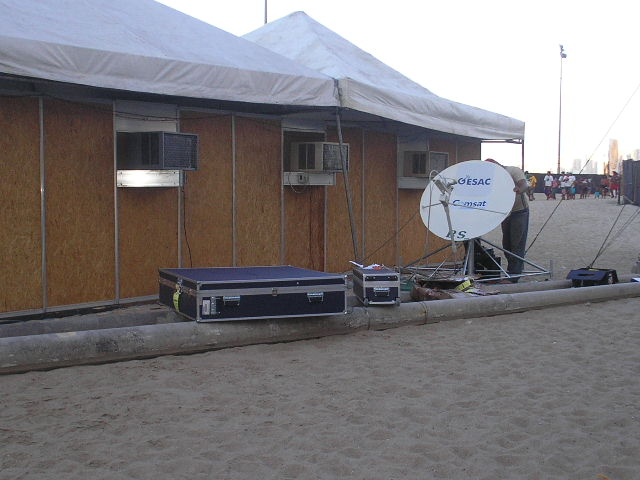
\includegraphics[max size={\textwidth}{\textheight}]{../../imagens/antenagesac.jpg}

	\end{center}

	\caption{\label{a3225c07ca3bc896130a8519e74f575fb919fefd}Antena Gesac, instalada nos jogos ind\'{i}genas.}

\end{figure}

Mas n\~ao bastava somente disponibilizar equipamentos tecnol\'ogicos, era imprescind\'{\i}vel que o programa contribu\'{\i}sse com a forma\c{c}\~ao dos usu\'arios no uso das TICS. Em 2004, entram em cena os  multiplicadores, conhecidos como implementadores sociais,  pessoas com habilidades t\'ecnicas,  que realizavam um trabalho de forma\c{c}\~ao  e apropria\c{c}\~ao das TICS juntos \`as comunidades atendidas pelo projeto.










O grupo de implementadores(as) sociais  passou por um processo de sele\c{c}\~ao e forma\c{c}\~ao sobre o programa. A escolha buscava identificar habilidades t\'ecnicas e sociais, com vistas \`a atua\c{c}\~ao em diversas comunidades, e par garantir pluralidade eram oriundos de todas as regi\~oes do Brasil. Eram preparados(as) para serem multiplicadores, passando por uma forma\c{c}\~ao que os permitisse aprender, dominar e compartilhar e disseminar o uso de software livre. Essas pessoas visitavam as comunidades de Norte a Sul do pa\'{\i}s, preparando e realizando oficinas. Entre as atividades que deveriam realizar estavam:











\begin{alineas}
\item instala\c{c}\~ao de laborat\'orios (as atividades inclu\'{\i}am, por exemplo, a implanta\c{c}\~ao do cabeamento da rede, migra\c{c}\~ao do software propriet\'ario para software livre, dentre outras atividades t\'ecnicas)
\item promo\c{c}\~ao de encontros locais e estaduais do programa,
\item colabora\c{c}\~ao para que os telecentros organizassem seu  comit\^e de gestor,
\item resolu\c{c}\~ao ou encaminhamento dos problemas  t\'ecnicos.
\end{alineas}

Os(as) implementadores(as) eram equipados com GPS, celular, notebook, projetor  e, al\'em do sal\'ario, tinham uma ajuda de custo para chegar aos rinc\~oes do Brasil. O papel das pessoas que atuavam na condi\c{c}\~ao de implementadores(as) era oferecer as oficinas de cultura digital, bem como colaborar para que a as pessoas, inseridas em suas comunidades, tivessem acesso e pudessem se apropriar das tecnologias da informa\c{c}\~ao e comunica\c{c}\~ao que estavam sendo disponibilizadas.










A  primeira gera\c{c}\~ao de implementadores  sociais foi composta por:











\begin{alineas}
\item Rafael Gomes da Cruz (Banto Palmarino)
\item Victor Reis,
\item Angel Lu\'{\i}s,
\item Tatiane Wells,
\item Isabela Toya,
\item Sergio Melo
\item Renata Louren\c{c}o,
\item Eduardo Aguiar,
\item Vincenzo Tozzi
\end{alineas}

Esses jovens percorreram as comunidades urbanas, rurais, quilombolas, ind\'{\i}genas e sem-terra ensinando e aprendendo com os atores envolvidos.










O primeiro v\'{\i}deo  (BAOBAXIA, 2003)  mostrando as oficinas do Gesac e do Programa Cultura Digital, que foram realizadas em Teresina/PI, Jo\~ao Pessoa, Brazlandia, Natal e Fortaleza, foi produzido por n\'os. O v\'{\i}deo mostra como se dava a atua\c{c}\~ao dos implementadores e o processo de forma\c{c}\~ao junto \`as comunidades envolvidas.










Com a viv\^encia obtida com a crescente implementa\c{c}\~ao do programa, listamos  algumas atribui\c{c}\~oes que os implementadores sociais deveriam ter em sua atua\c{c}\~ao junto aos Pontos de Presen\c{c}a. Estas atribui\c{c}\~oes foram definidas como a\c{c}\~oes b\'asicas, desej\'aveis e necess\'arias. Essas atribui\c{c}\~oes constam da disserta\c{c}\~ao da Profa. Ana Val\'eria Machado Mendon\c{c}a  (MENDON\c{C}A, 2015) e s\~ao reproduzidas abaixo:











\begin{alineas}
\item Conectar e dialogar com os administradores estaduais e regionais dos Pontos de Presen\c{c}a, visando estabelecer estrat\'egias para aperfei\c{c}oar o trabalho;
\item intermediar e propor parcerias, em co-responsabilidade com a equipe do MC; e Relacionamento com as Comunidades;
\item forma\c{c}\~ao e capacita\c{c}\~ao no uso das ferramentas GESAC;
\item apontar a  necessidade de remanejamento de antena para o MC;
\item criar condi\c{c}\~oes de manuten\c{c}\~ao t\'ecnica;
\item realizar migra\c{c}\~ao de software propriet\'ario para software livre;
\item metareciclagem: aproveitamento de m\'aquinas velhas colocadas em rede;
\item verificar a qualidade da conex\~ao (ping, teste de taxa de download, FTP...);
\item verificar a funcionalidade da rede local LAN;
\item identificar problemas de cabeamento, sugerir poss\'{\i}veis solu\c{c}\~oes e implement\'a-las;
\item incentivar a forma\c{c}\~ao de um Conselho Gestor no Ponto de Presen\c{c}a;
\end{alineas}

Os implementadores planejavam seus trabalhos e as visitas usando uma ferramenta wiki, bem como, apresentando mensalmente seus relat\'orios de atividades.










A coordena\c{c}\~ao de Relacionamento com as Comunidades – REL- era respons\'avel por coordenar os trabalhos dos(as) implementadores. Essa fun\c{c}\~ao era ocupada por essa candidata ao mestrado,  juntamente com os colegas, Toni Klaus Bochat, Alcione  Gabriel da Silva, Ana Val\'eria Machado Mendon\c{c}a e \'Alvaro Malagute.










O GESAC conectou os Pontos de Presen\c{c}as em diversas comunidades, institui\c{c}\~oes governamentais, da sociedade civil, de movimentos sociais e outras iniciativas de inclus\~ao digital. Para  atender a diversidade de parcerias  e de outros programas em curso, como, por exemplo, do Programa Cultura Viva e levar as  capacita\c{c}\~oes no uso das tecnologias da informa\c{c}\~ao e comunica\c{c}\~ao, organizamos encontros estaduais de forma\c{c}\~ao, conhecidos como Encontros de Conhecimentos Livres, realizados em todos os estados do Brasil. Ocorreram, ainda, as  oficinas de inclus\~ao digital com as redes de ensino e organiza\c{c}\~oes sociais.










O primeiro encontro estadual de forma\c{c}\~ao ocorreu em  Teresina, Piau\'{\i}, junto com o Programa Cultura Viva. A partir deste, os demais estados passaram a organizar seus encontros, sempre com a participa\c{c}\~ao da equipe do GESAC.










Al\'em das oficinas estaduais e dos locais de forma\c{c}\~ao, o GESAC tamb\'em organizava encontros com os gestores estaduais para planejar as a\c{c}\~oes nos estados. Assim, foram organizados encontros com as redes de ensino e  representantes da sociedade civil, pois cada ponto  tinha seu Comit\^e de Gestor.










Elaboramos, a partir destas viv\^encias, o Manual do Usu\'ario do Programa GESAC, editado pelo Minist\'erio das Comunica\c{c}\~oes (MC, 2008).










O Manual do GESAC visava a orientar as atividades pedag\'ogicas das oficinas realizadas nos Pontos de Presen\c{c}a, bem como as  atividades rotineiras de funcionamento dos equipamentos e aplicativos.










O conte\'udo do manual inclu\'{\i}a informa\c{c}\~oes:











\begin{alineas}
\item sobre o pr\'oprio GESAC, sua estrutura e organiza\c{c}\~ao,
\item sobre o funcionamento da conex\~ao via sat\'elite VSAT, a banda larga usada pelo programa,
\item sobre a cestas de servi\c{c}os dispon\'{\i}veis no Portal IDBRASIL, destacando as regras de uso dos servi\c{c}os,
\item sobre os canais de comunica\c{c}\~ao para atendimento das comunidades, dado que o programa provia um \textquotedbl Fale conosco\textquotedbl .
\item sobre o correio eletr\^onico disponibilizado,
\item sobre a TEIA, blogs, listas de discuss\~ao, editor de HTML, NVU, RAU-TU, WIKI, VOIP, MULTICAST, com respectivo gloss\'ario.
\end{alineas}

O primeiro ponto instalado do Governo Eletr\^onico foi no Piau\'{\i}, em 2003, portanto, seis meses ap\'os a posse do novo governo. A primeira vers\~ao do GESAC previa 3,2 mil pontos, e cada local de instala\c{c}\~ao recebia de 15 a 20 computadores. O GESAC chegou a ter mais de 30 mil m\'aquinas conectadas em rede. N\~ao existia nenhum programa dessa ordem de grandeza no Brasil. A previs\~ao de 3,2 mil m\'aquinas foi amplamente superada e chegou-se a mais de 30 mil m\'aquinas.










Segundo Ant\^onio Albuquerque, entrevistado por n\'os,











\noindent\begin{center}\mbox{\centering\fbox{\centering\par\parbox{0.7\linewidth}{\small\textit{\textquotedbl Tudo era muito diif\'{\i}cil no in\'{\i}cio do projeto, pela sua magnitude, num pa\'{\i}s continental, para fazer e executar esse projeto. A solu\c{c}\~ao foi tornar o GESAC um programa de programas, que aproximasse pequenas iniciativas de inclus\~ao digital.\textquotedbl  (trecho de entrevista concedida para esta autora por Ant\^onio Albuquerque)}\normalsize}}}\end{center}


Este entendimento do gestor do GESAC criou as condi\c{c}\~oes para a articula\c{c}\~ao de v\'arias iniciativas, principalmente com programas locais que n\~ao tinham acesso \`a internet, mas que j\'a estavam trabalhando com computadores.










Foi a partir desse entendimento que o GESAC passou a fazer parcerias com os minist\'erios da Defesa, com o MEC, com o MCDIC,  Minist\'erio da Sa\'ude e diversas ONGS, dentre as quais destacam-se a \textquotedbl Sa\'ude e Alegria\textquotedbl   no Amazonas e a \textquotedbl Casa de Cultura Tain\~a\textquotedbl , com \^enfase nas comunidades quilombolas, por meio da Rede Mocambos, bem como muitas outras no semi-\'arido.










No Minist\'erio da Cultura, que estava sendo estruturado pelo m\'usico Gilberto Gil, com apoio de C\'elio Turino, o Programa GESAC buscou integrar-se aos programas \textquotedbl Cultura Viva\textquotedbl  e \textquotedbl Pontos de Cultura\textquotedbl .











\noindent\begin{center}\mbox{\centering\fbox{\centering\par\parbox{0.7\linewidth}{\small\textit{“Esse foi um programa muito importante, com o qual tivemos uma importante aproxima\c{c}\~ao. E n\'os levamos o GESAC para in\'umeros pontos de cultura, em todo o Brasil. Com os Pontos de Cultura, t\'{\i}nhamos um elemento digital muito importante. Cada ponto recebia uma m\'aquina fotogr\'afica, filmadoras e internet para subir os conte\'udos produzidos. Estamos falando de tempos  em que n\~ao existia a produ\c{c}\~ao audiovisual disseminada como \'e hoje. Essa somat\'oria de programas e complementariedades foi muito grande. Fizemos parcerias, ainda, com o Minist\'erio do Planejamento, com a Rede Mocambos, n\'os colocamos o projeto em mais de 90 comunidades quilombolas. Onde n\~ao existia conex\~ao de internet, n\'os chegamos com conex\~ao, via sat\'elite. A rede Mocambos se institucionalizou no campo da comunica\c{c}\~ao gra\c{c}as ao GESAC. Comunidades ind\'{\i}genas, tamb\'em. N\'os fizemos um trabalho muito importante com a Eletronorte para colocar pontos em comunidades ind\'{\i}genas, onde n\~ao havia energia el\'etrica para fazer a internet funcionar. A Eletronorte chegou com placas de energia solar, que alimentavam o sat\'elite e os computadores. O GESAC levou a internet em palho\c{c}as de taipa, que passaram a contar com o que n\~ao era nem sonhado.” (ALBUQUERQUE, depoimento, coletado  em setembro de 2022).}\normalsize}}}\end{center}


O GESAC ganhou premia\c{c}\~oes e reconhecimento pelo trabalho. Recebeu o Pr\^emio de Melhores Experi\^encias de Gest\~ao P\'ublica e venceu o pr\^emio entre as cinco melhores experi\^encias da ENAP (Escola Nacional de Administra\c{c}\~ao P\'ublica), vinculada ao Minist\'erio da Economia.










O GESAC, no governo federal, foi a primeira experi\^encia de fazer um programa de inclus\~ao digital numa escala continental, n\~ao s\'o pensando no acesso, mas na gera\c{c}\~ao de conte\'udo. Para isso, teve que desenvolver um m\'etodo de educa\c{c}\~ao. Ele teceu uma grande rede de institui\c{c}\~oes e atores, que  implementaram  a cultura digital, envolvendo os entes federados, as redes de ensino  e a sociedade civil,  contribuindo, assim, com a sociedade da informa\c{c}\~ao.










Como se ver\'a na discuss\~ao final, esse modelo implantado pelo GESAC teve forte influ\^encia na concep\c{c}\~ao do WASH, dado que aquele programa, posterior, tamb\'em buscou se valer do conceito de multiplicadores e de uma estrutura de funcionamento heter\'arquica. No WASH e no GESAC, o trabalho \'e mobilizar atores locais, fornecendo o m\'etodo de trabalho e os multiplicadores, que permitir\~ao disseminar esse m\'etodo. Diferentemente do WASH, o GESAC tinha uma \^enfase maior em disponibiliza\c{c}\~ao de infraestrutura de equipamentos e redes, situa\c{c}\~ao que o WASH n\~ao teve que enfrentar, justamente pelo trabalho pr\'e-existente, que dotou muitos equipamentos p\'ublicos com internet.










Um importante diferen\c{c}a entre o WASH e o GESAC \'e o p\'ublico alvo dos dois programas. Enquanto o GESAC n\~ao define um alvo em termos de faixa et\'aria, o WASH \'e voltado para estudantes do ensino fundamental e m\'edio. As semelhan\c{c}as e diferen\c{c}as entre os dois programas ser\~ao elencadas ao final deste cap\'{\i}tulo, como base para a busca de elementos comuns entre os dois programas.












\captionsetup{format=plain}
\begin{figure}[max size={\textwidth}{\textheight}]

\centering


\begin{minipage}[b]{0.4\linewidth}
        \centering
                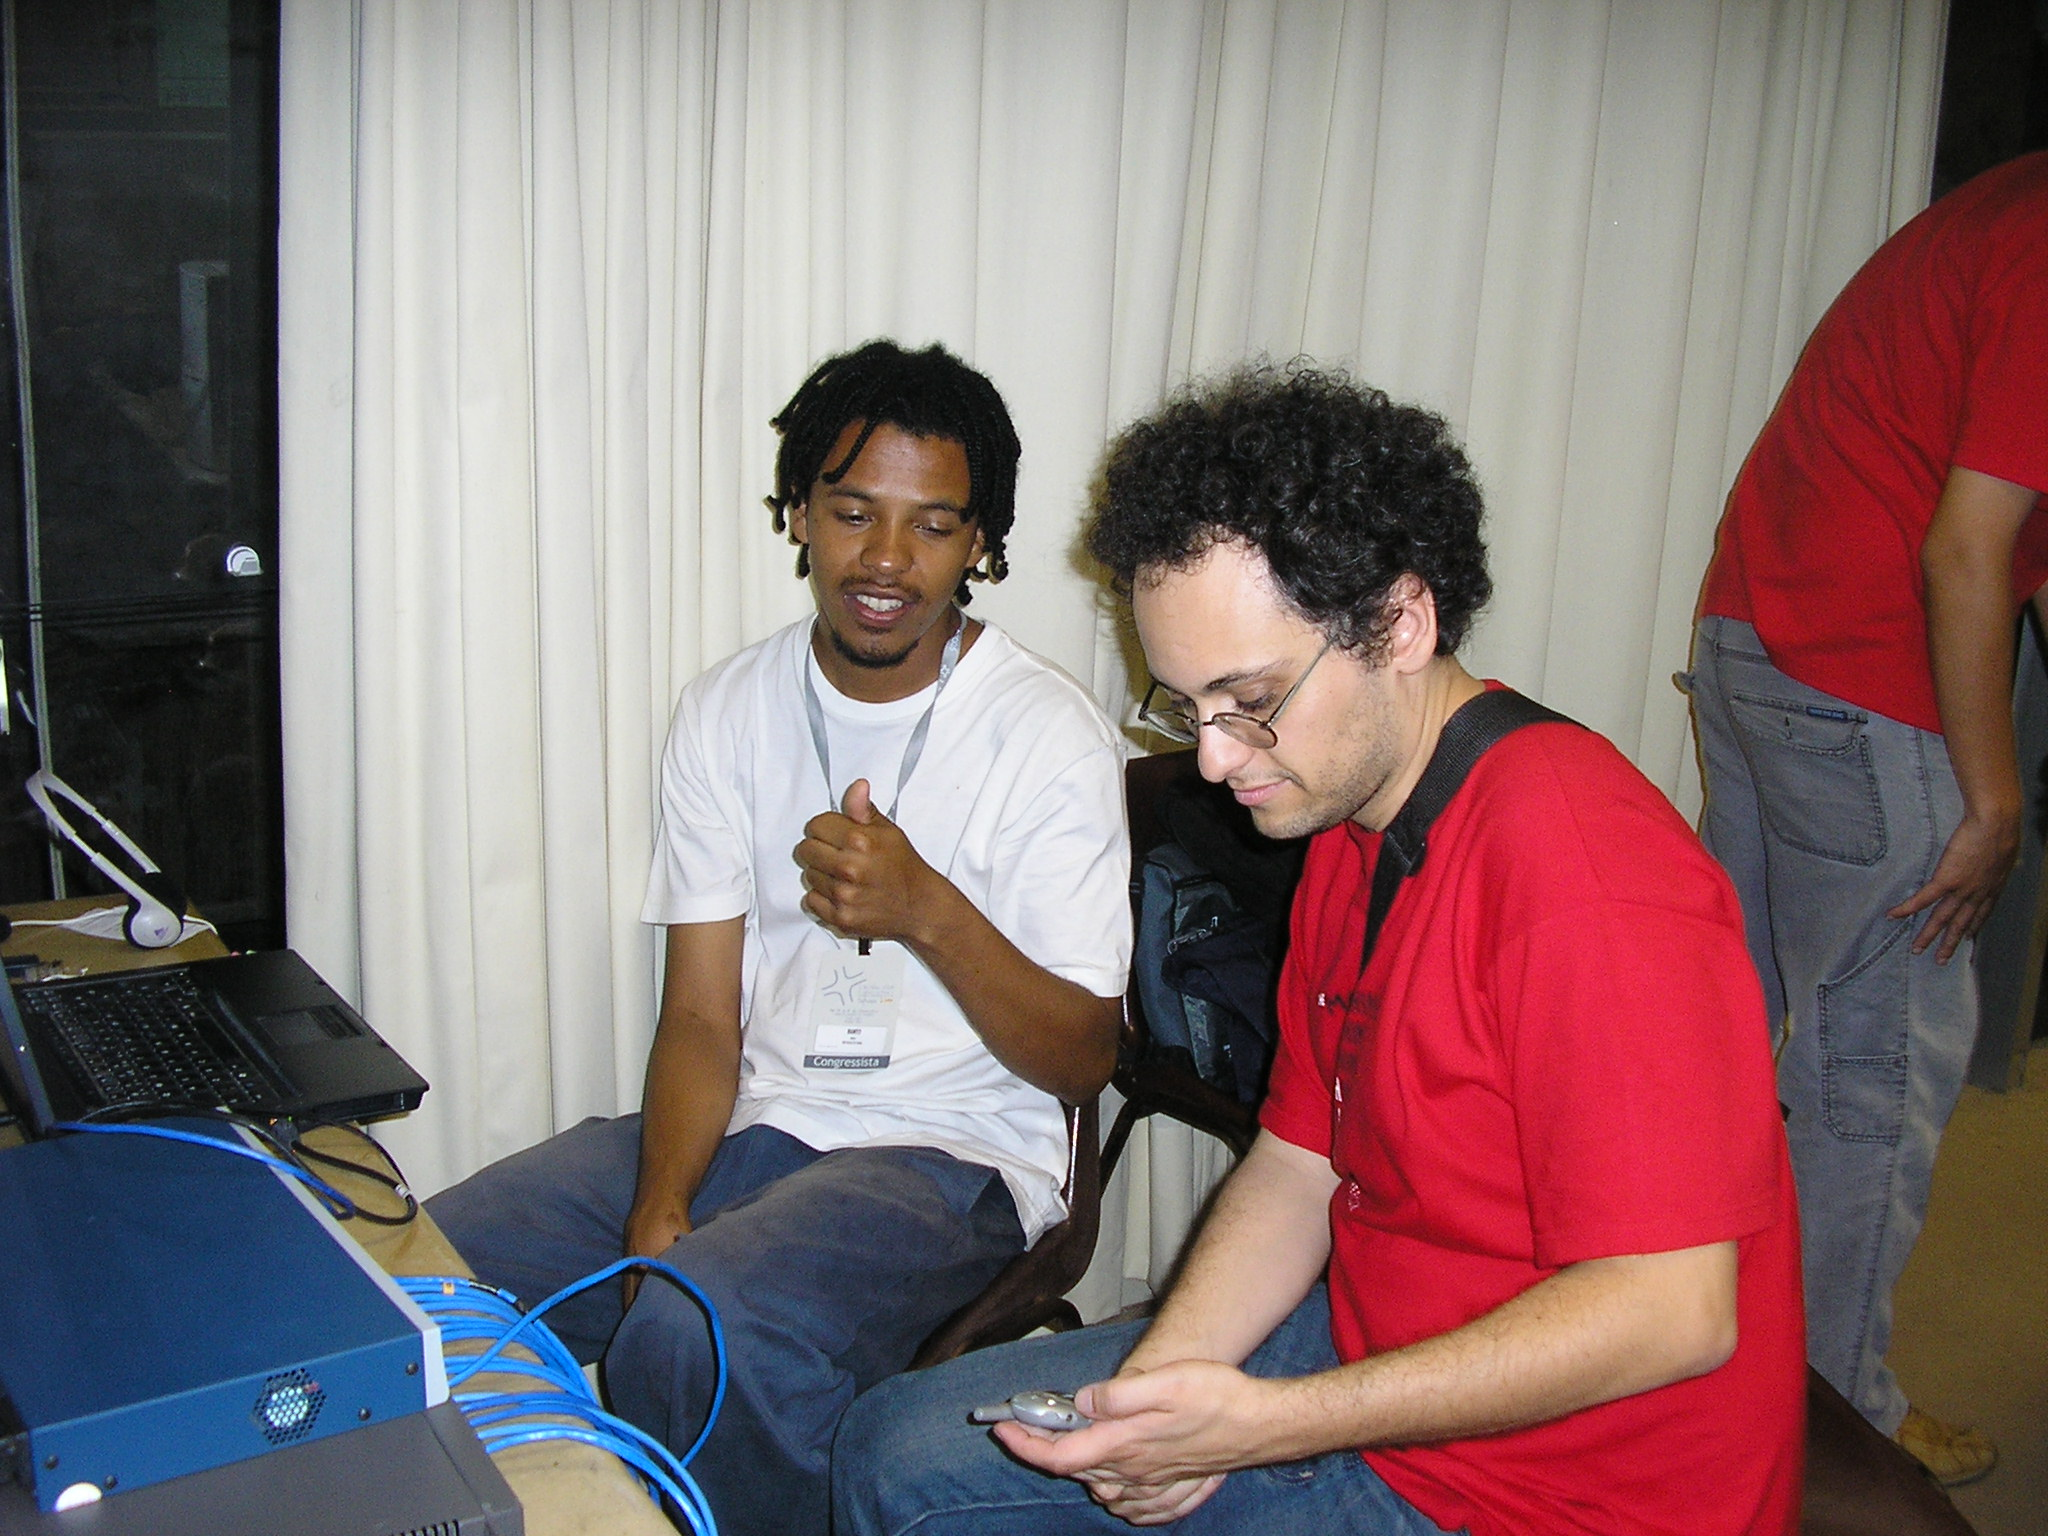
\includegraphics[width=1.0\linewidth]{../../imagens/bantorafa.JPG}
                \caption{Oficina de forma\c{c}\~ao de implementadores(as). Na foto v\^e-se Rafael Gomes da Cruz (i.e. Banto Palmarino) e XXX. Banto foi posteriormente integrado `a equipe do WASH, trazendo para o novo programa a experi\^encia de multiplica\c{c}\~ao do GESAC.}
                \label{d2d74ac61c1b95a746858e8420d24348e1b48f51}
\end{minipage}%
\hspace{0.5cm}
\begin{minipage}[b]{0.4\linewidth}
        \centering
                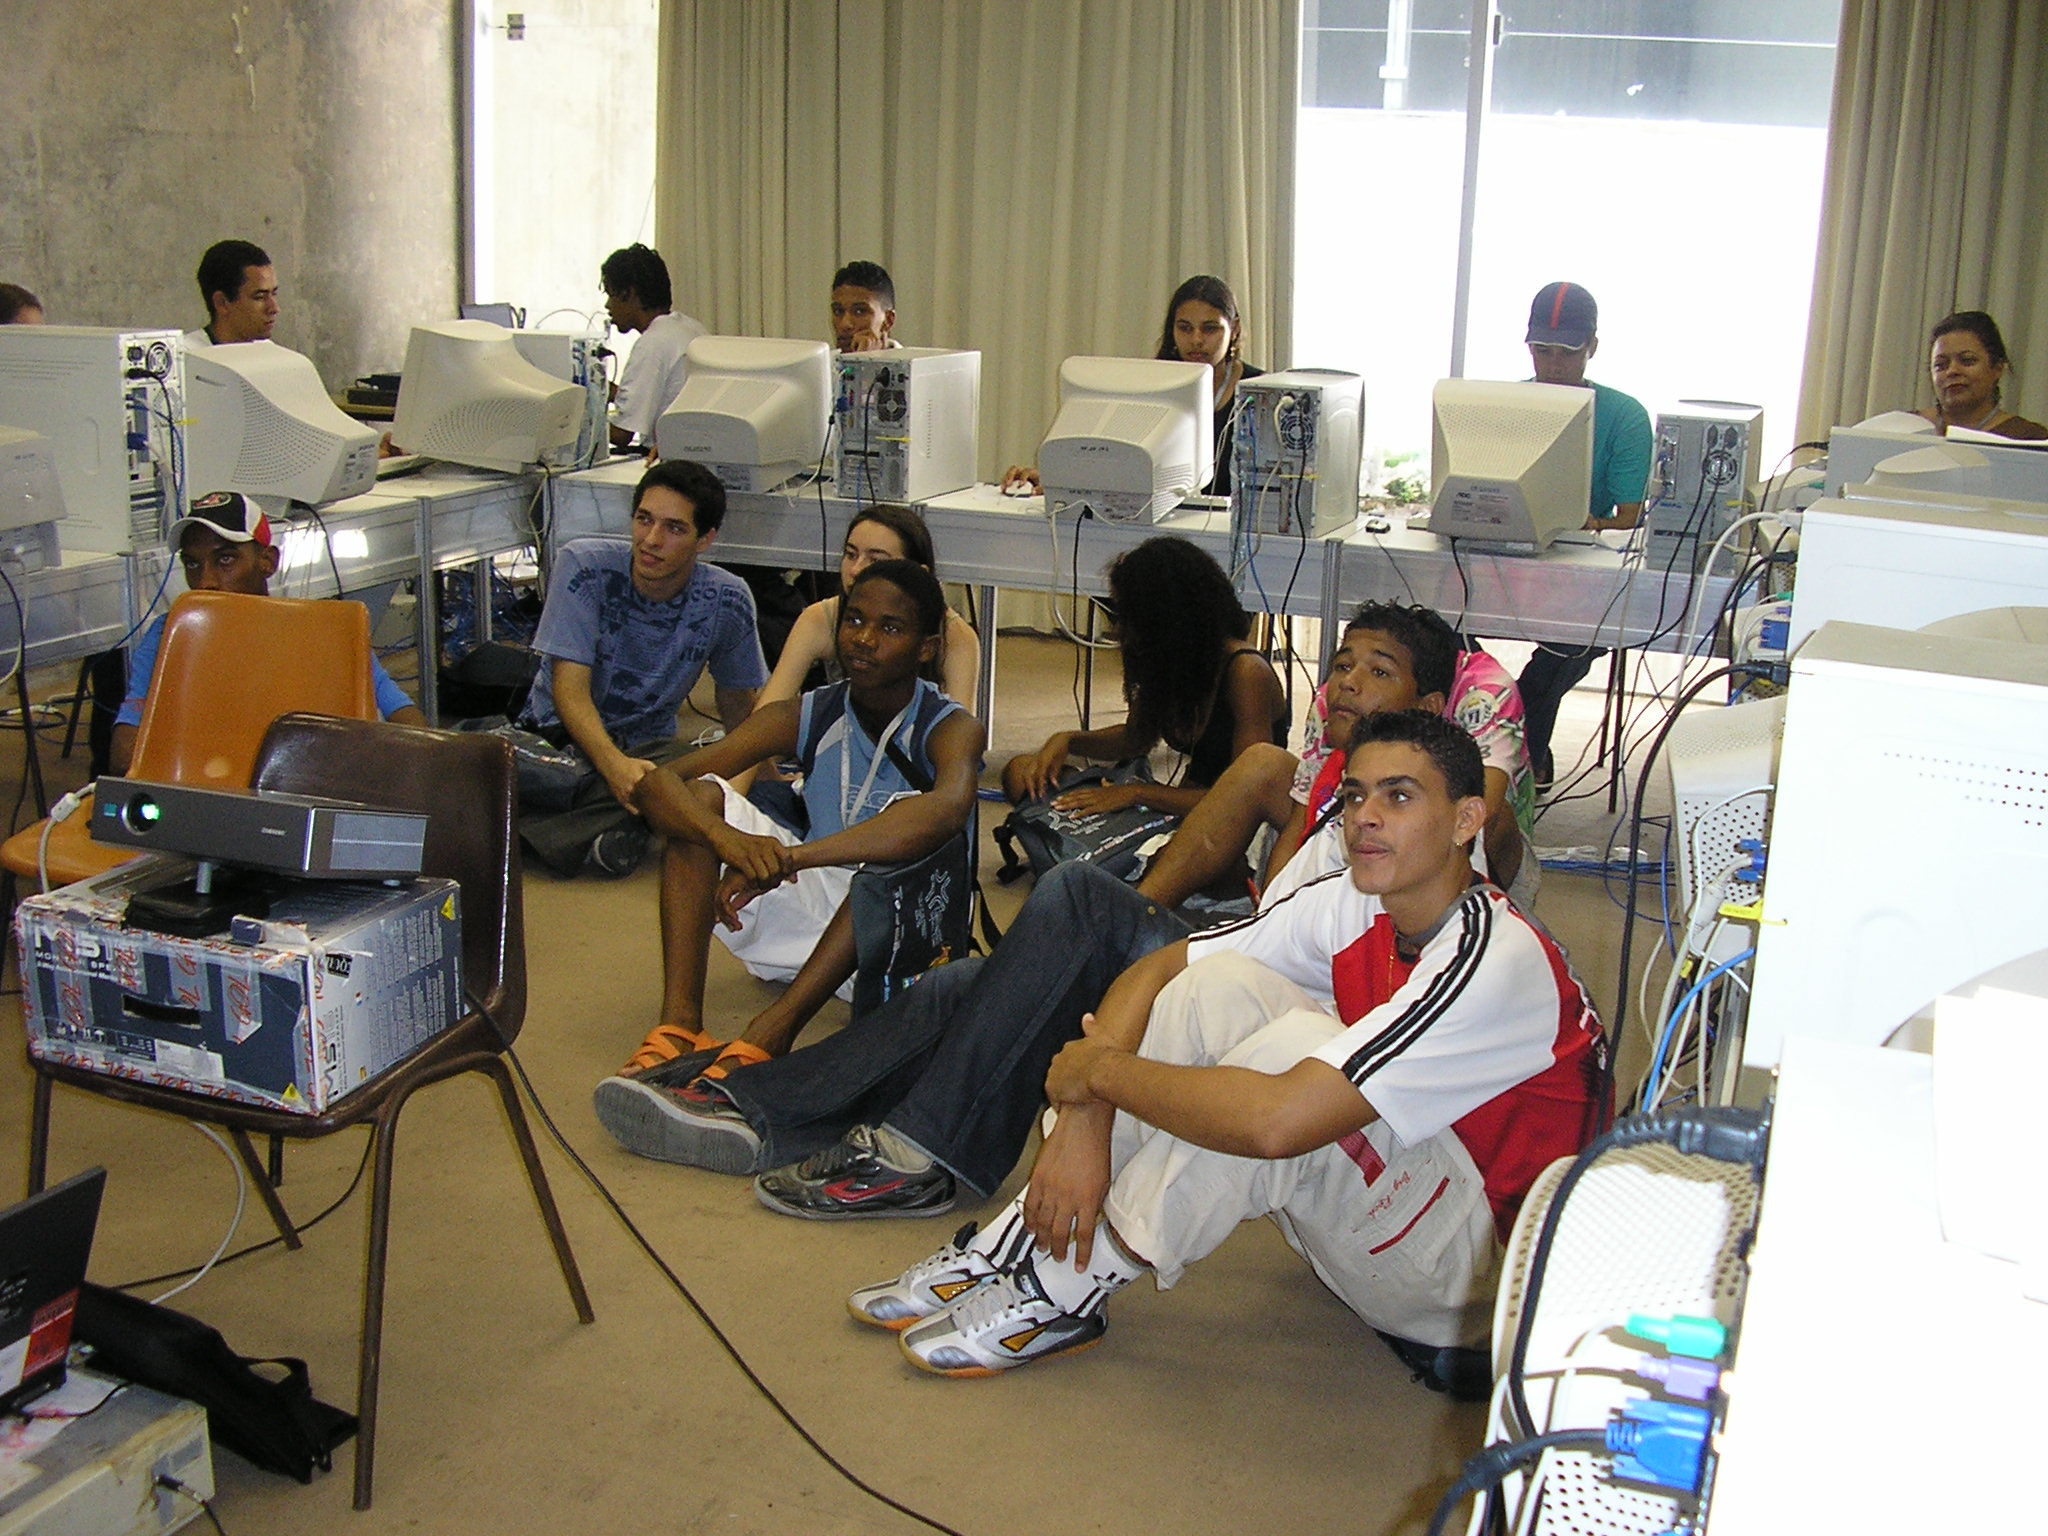
\includegraphics[width=1.0\linewidth]{../../imagens/oficinalac.JPG}
                \caption{Oficina LacFree do GESAC, baseada sempre em conhecimentos livres.}
                \label{350ae75fda8eb19905317e70b64079af869125d8}
\end{minipage}
\hspace{0.5cm}
\begin{minipage}[b]{0.4\linewidth}
        \centering
                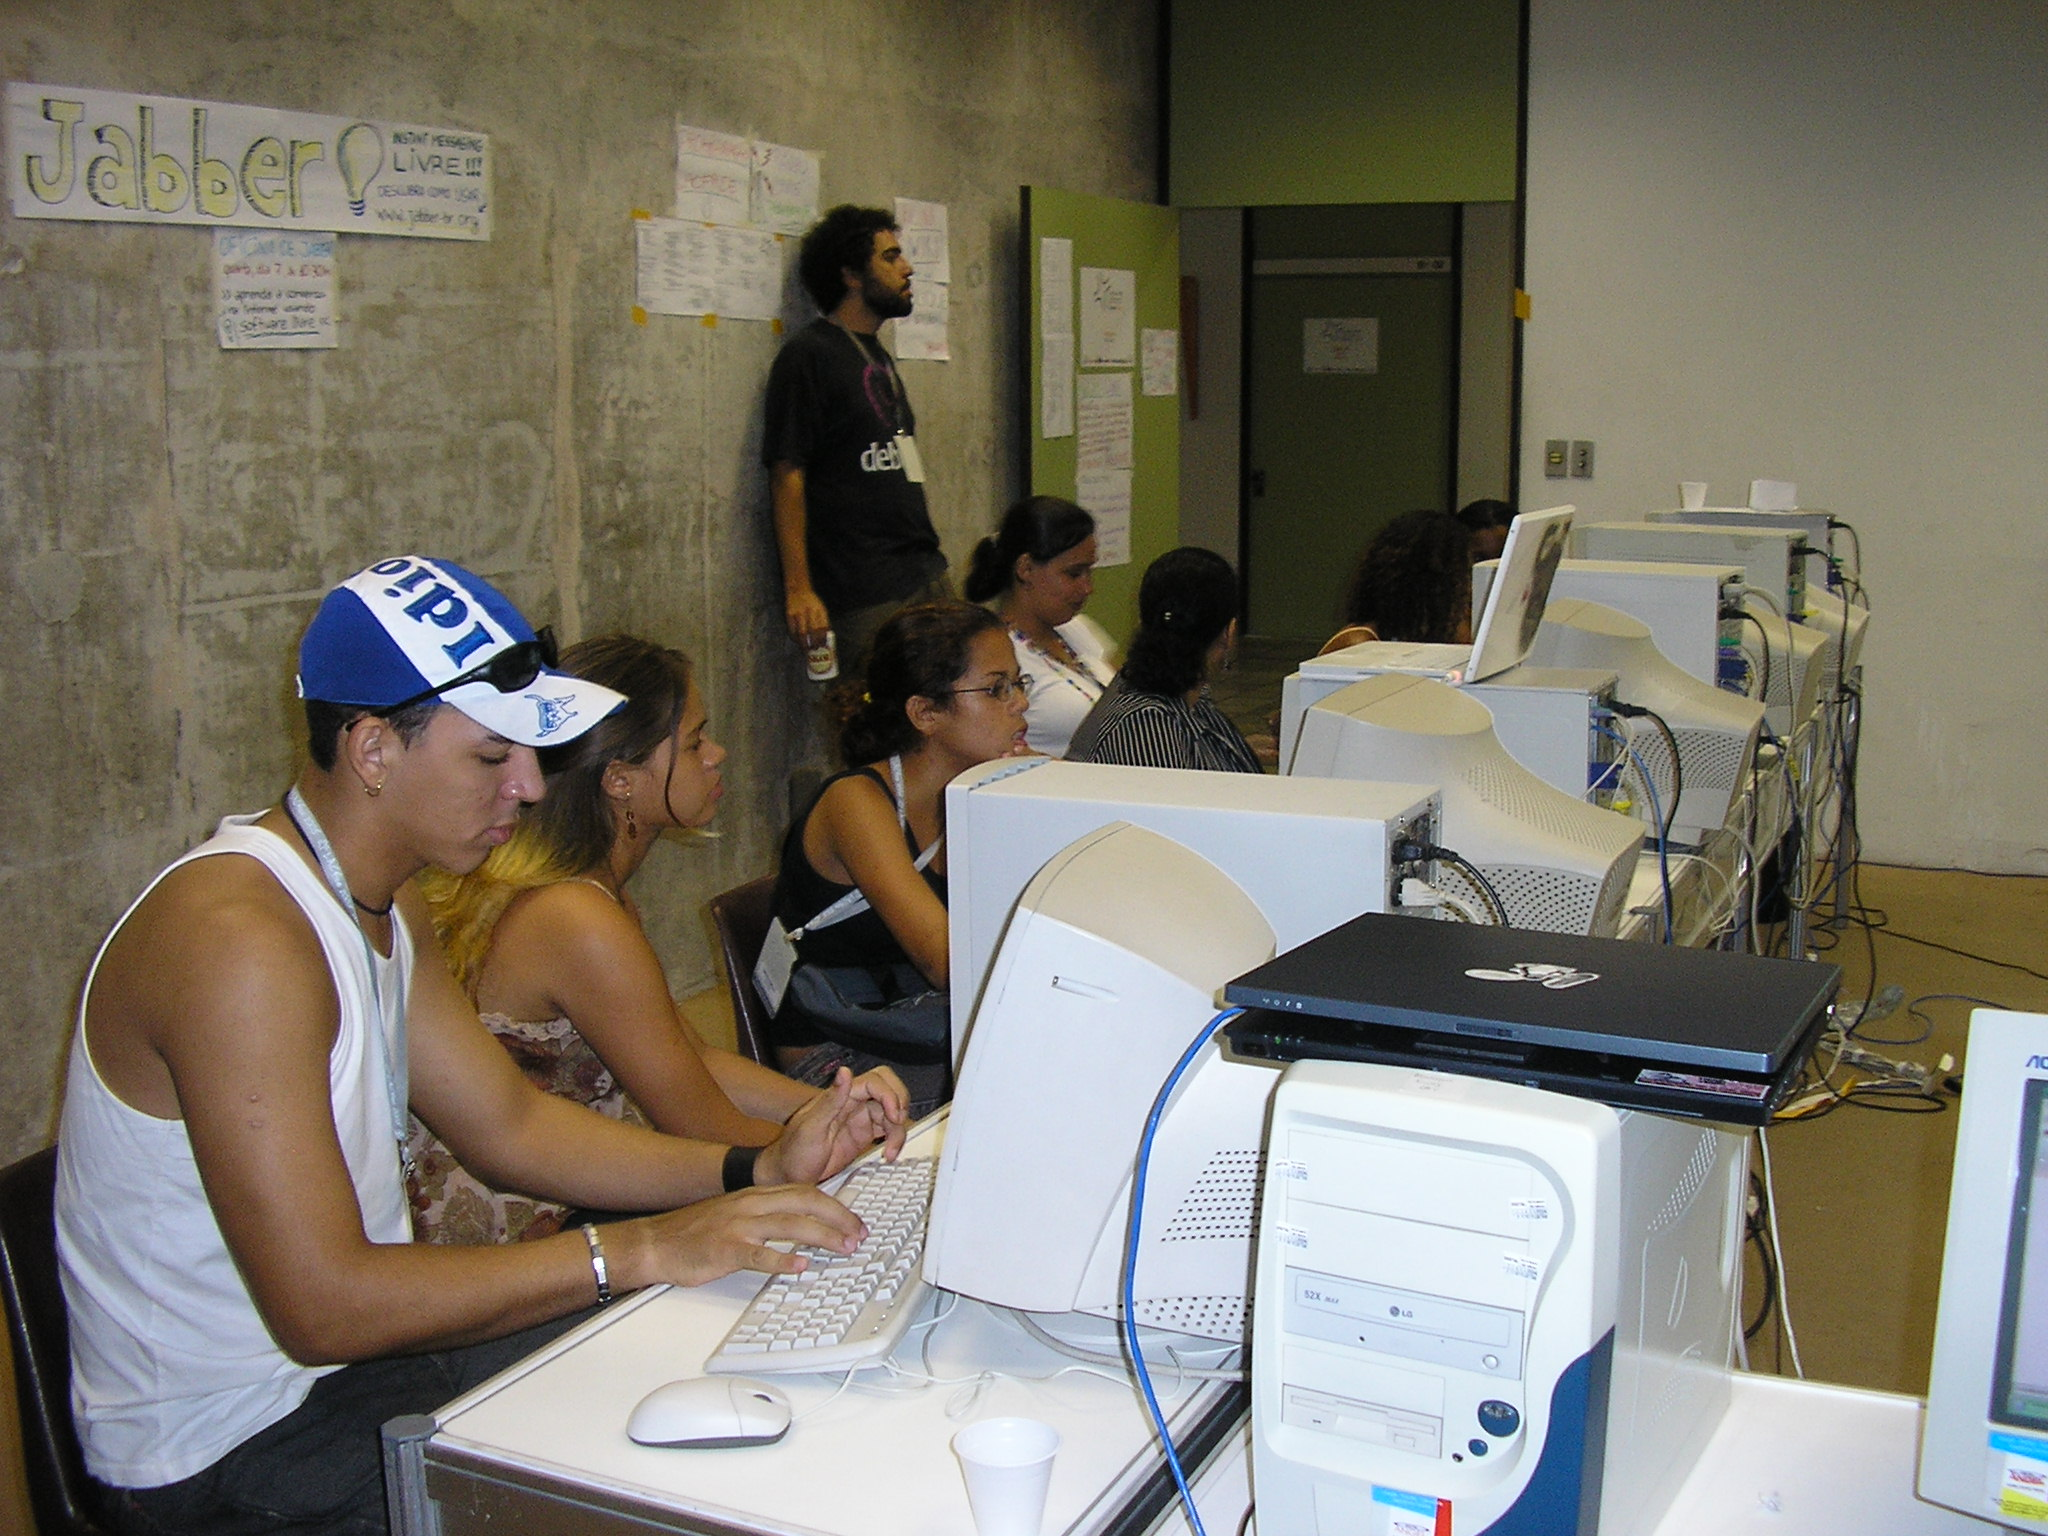
\includegraphics[width=1.0\linewidth]{../../imagens/jabber.JPG}
                \caption{Oficina de Jabber com gestores.}
                \label{e29d9c3f5a4aa82fa420bc60ed161880a24bc2b6}
\end{minipage}%
\hspace{0.5cm}
\begin{minipage}[b]{0.4\linewidth}
        \centering
                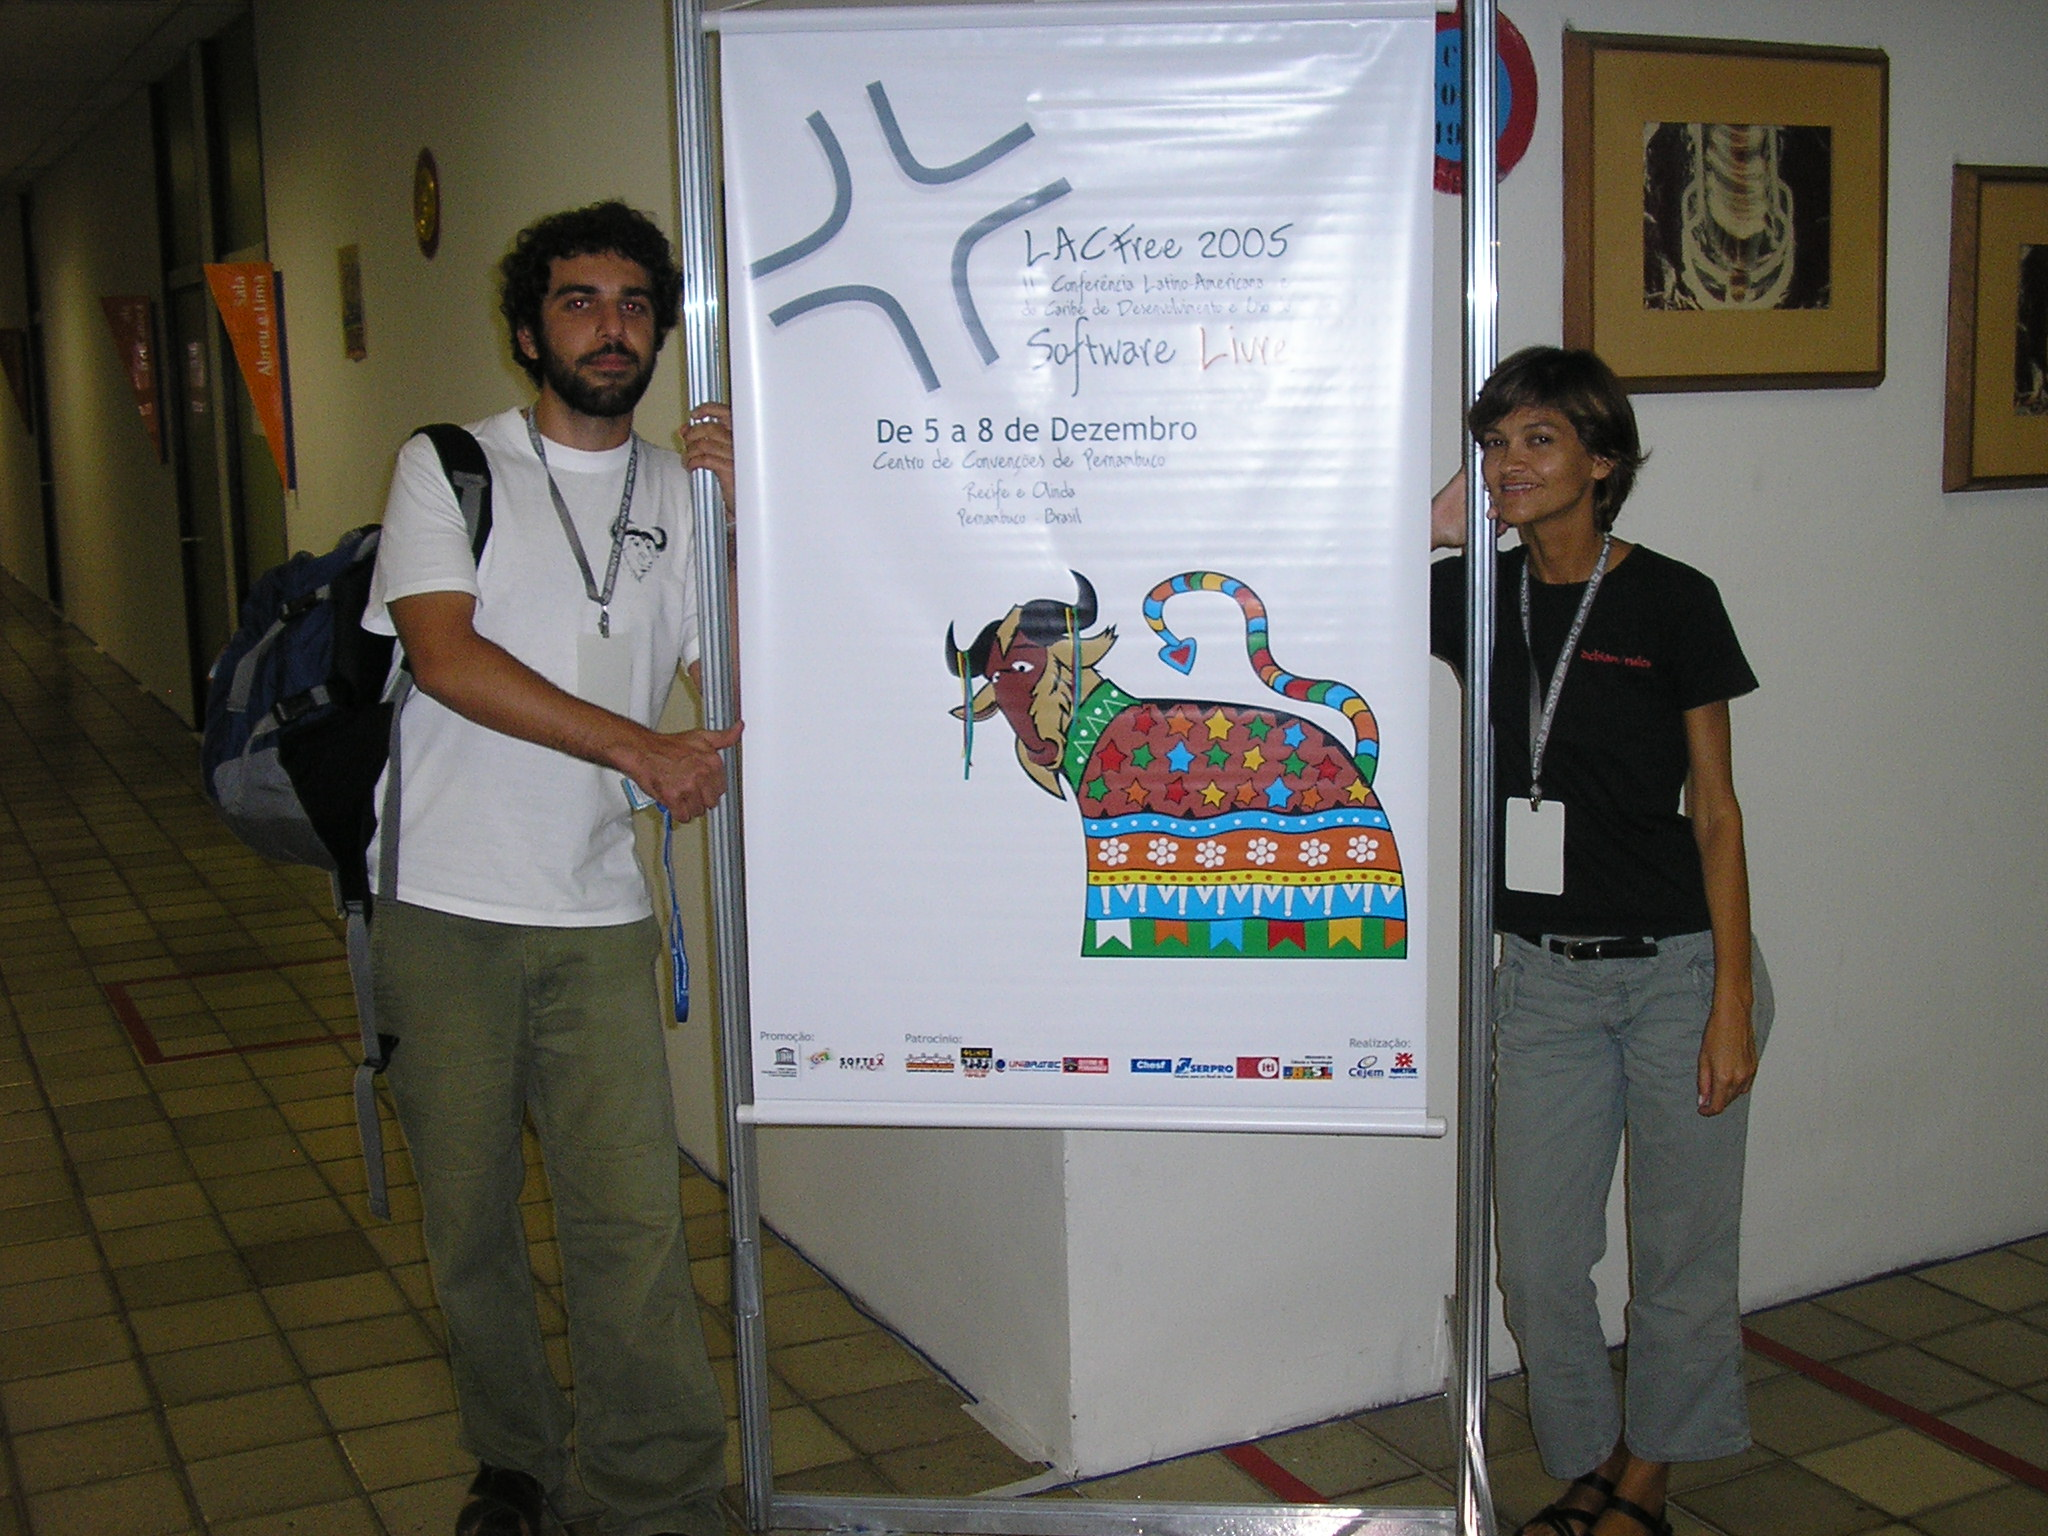
\includegraphics[width=1.0\linewidth]{../../imagens/lacelavince.JPG}
                \caption{A presente candidata, ao lado de Vincenzo Tozzi, implementador que tamb\'em veio a contribuir com o WASH.}
                \label{4459669909728990ef00df4bdb6a369f3449704e}
\end{minipage}
\hspace{0.5cm}
\begin{minipage}[b]{0.4\linewidth}
        \centering
                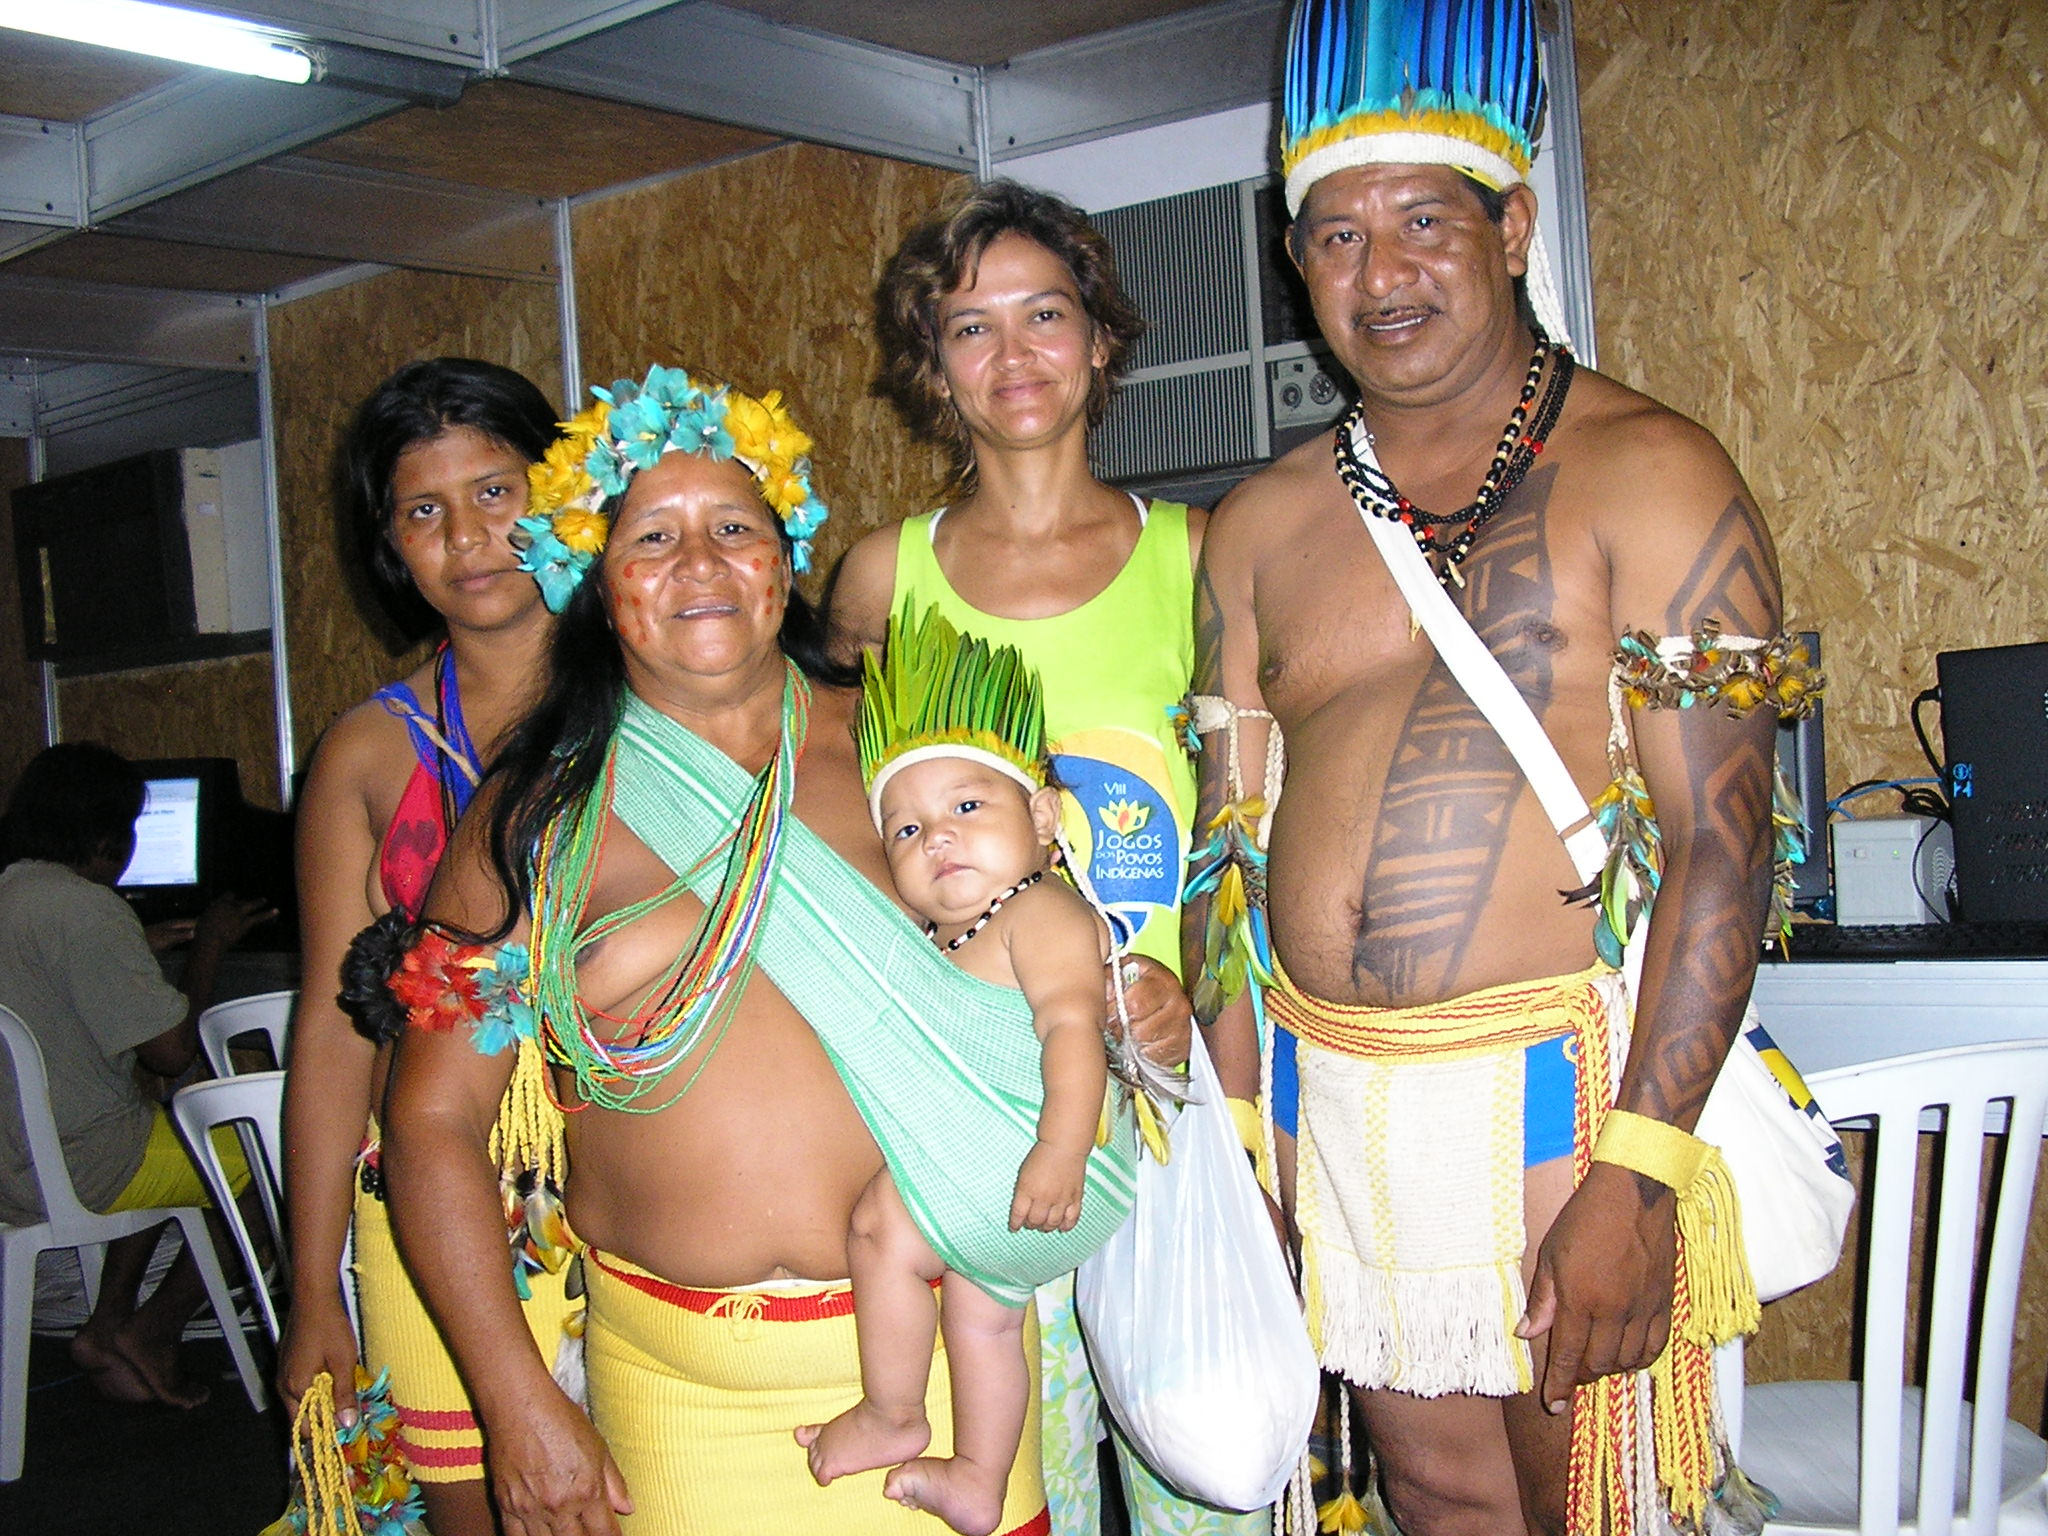
\includegraphics[width=1.0\linewidth]{../../imagens/povo.JPG}
                \caption{Oficinas em comunidades ind\'{i}genas eram muito comuns no GESAC.}
                \label{50c13a4f82feece9e41db915d8e5bc4c5d5094dd}
\end{minipage}%
\hspace{0.5cm}
\end{figure}



\subsection[Avalia\c{c}\~ao do OLPC e PID como g\^enese do WASH]{Avalia\c{c}\~ao do OLPC e PID como g\^enese do WASH}\label{Avalia\c{c}\~ao do OLPC e PID como g\^enese do WASH}
Nesta se\c{c}\~ao fazemos uma interpreta\c{c}\~ao sobre a g\^enese do Programa WASH, a partir do acervo de documentos por n\'os levantado. Nesta parte utilizaremos, principalmente (mas n\~ao exclusivamente), os documentos referentes a duas avalia\c{c}\~oes conduzidas pelo Coordenador do Projeto WASH na primeira d\'ecada deste s\'eculo:











\begin{alineas}
\item Avalia\c{c}\~ao do Projeto \textquotedbl One Laptop per Child\textquotedbl  (OLPC), e sua vers\~ao brasileira, \textquotedbl Projeto Um Computador por Aluno\textquotedbl  (UCA)  (MAMMANA, 2006)
\item Avalia\c{c}\~ao do Programa de Inclus\~ao Digital (PID) da Secretaria de Inclus\~ao Social do Minist\'erio da Ci\^encia e Tecnologia  (CGEE, 2010a)
\end{alineas}

O Projeto \textquotedbl One Laptop Per Child\textquotedbl  (NEGROPONTE, 2004) foi uma das iniciativas mais completas e robustas no sentido de ampliar a escala de aplica\c{c}\~ao das ideias de Papert. Ao mesmo tempo, era bastante pol\^emica (ALVAREZ, 2015) por suas caracter\'{\i}sticas disruptivas, alcance e ambi\c{c}\~ao de crescimento (MAMMANA e TOZZI, 2018).










Embora o Projeto OLPC estivesse no \^ambito de uma Organiza\c{c}\~ao n\~ao-Governamental independente,  foi concebido por pesquisadores do Massachusetts Institute of Technology (MIT), apoiados nas ideias e experi\^encias de Seymour Papert  (ALVAREZ, 2015). Especificamente, o Projeto OLPC \'e resultado das ideias debatidas por muitos anos no \^ambito do Media Lab, laborat\'orio do MIT, do qual Papert foi Presidente do Conselho e Co-Fundador  (ALVAREZ, 2015).










Os proponentes do OLPC tinham a ambi\c{c}\~ao de que suas ideias fossem adotadas por pa\'{\i}ses em desenvolvimento e, para isso, estabeleceram planos para regi\~oes espec\'{\i}ficas do mundo, a exemplo do Brasil.










Em 2005, Nicholas Negroponte, idealizador do Projeto OLPC, apresentou sua ideia em Davos (MARKOFF, 2005). Naquela oportunidade, encontrou-se com representantes do Governo Brasileiro (ALVAREZ, 2015) que organizaram um encontro com o Presidente Lula, o qual foi realizado em junho daquele ano (ALVAREZ, 2015) (CRISTINA, 2005).










Como resultado dessas tratativas iniciais, o documento entitulado \textquotedbl Brazil Plan\textquotedbl   (NEGROPONTE, 2004), fonte prim\'aria para a constru\c{c}\~ao da presente narrativa, foi direcionado \`a \textquotedbl Brazilian Task Force\textquotedbl , tendo sido compartilhado com governo brasileiro em 2005.










O OLPC era explicitamente apoiado por Papert, quando ainda estava vivo, tendo contado com sua presen\c{c}a ativa e eloquente nas reuni\~oes de apresenta\c{c}\~ao do OLPC para o Governo Brasileiro, inclusive numa visita ao presidente Lula (ver fig. XXX).












\captionsetup{format=plain}
\begin{figure}[max size={\textwidth}{\textheight}]

\centering


\begin{minipage}[b]{0.4\linewidth}
        \centering
                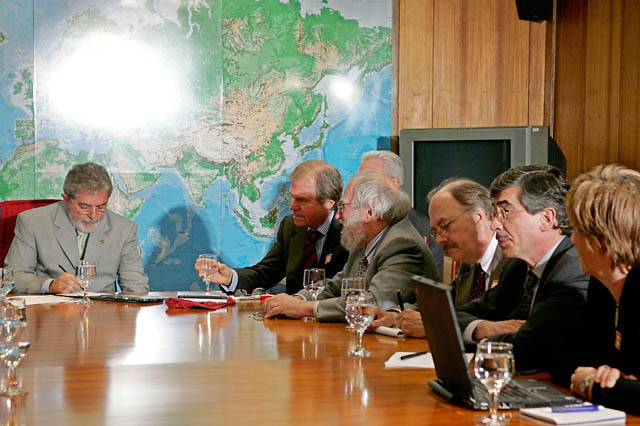
\includegraphics[width=1.0\linewidth]{../../imagens/lula-papert.jpg}
                \caption{Presidente Lula, Negroponte, Papert, Rodrigo Mesquita e Mary Lou Kepsen (fonte: flicker de Rodrigo Mesquita).}
                \label{7c0febad22b3e599a6886b31cdcbd3be3ce60df2}
\end{minipage}%
\hspace{0.5cm}
\begin{minipage}[b]{0.4\linewidth}
        \centering
                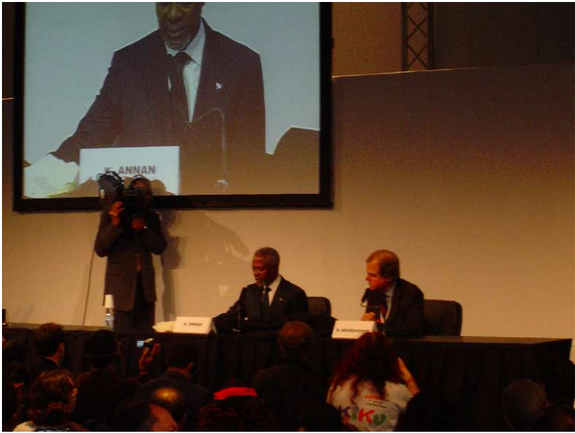
\includegraphics[width=1.0\linewidth]{../../imagens/Kofi-negroponte.png}
                \caption{Nicholas Negroponte apresentando o prot\'otipo do OLPC para o Secret\'ario Geral da ONU, Kofi Anan (cr\'edito: Victor Mammana, 2005).}
                \label{31f6206a8e4662597d5a134974d64a4696f4129c}
\end{minipage}
\hspace{0.5cm}
\begin{minipage}[b]{0.4\linewidth}
        \centering
                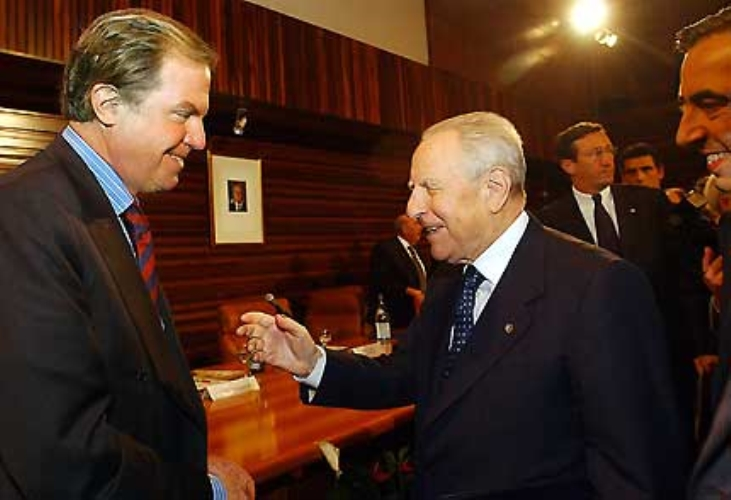
\includegraphics[width=1.0\linewidth]{../../imagens/presidente-italia.jpg}
                \caption{Nicholas Negroponte com o presidente da It\'alia, em 2003.}
                \label{f15f5d2fa7b78d2e6dec6ac4a7be76d564c9bf71}
\end{minipage}%
\hspace{0.5cm}
\end{figure}



Nicholas Negroponte, o l\'{\i}der da iniciativa do OLPC, era um destacado \textquotedbl gur\'u\textquotedbl  tecnol\'ogico, professor do MIT, co-fundador da revista Wired e tinha acesso a chefes de estado, a exemplo do presidente Miterrand da Fran\c{c}a, que na d\'ecada de 80 foi apoiador da cria\c{c}\~ao do \textquotedbl Centre mondial informatique et ressource humaine\textquotedbl , onde Negroponte atuou como dirigente. Coincidentemente, era irm\~ao de John Negroponte, ent\~ao Secret\'ario de Estado do Governo Bush, diplomata americano influente nos meios pol\'{\i}ticos, na comunidade de informa\c{c}\~ao e em outras \'areas estrat\'egicas e de defesa daquele pa\'{\i}s.










Nicholas transitava com razo\'avel desenvoltura entre l\'{\i}deres mundiais, a exemplo de Kofi Anan, Lula, Mitterrand ou o presidente da It\'alia (ver fig. XXX). Essa presen\c{c}a junto a governos criou a oportunidade para que, em 2006, pa\'{\i}ses como Argentina, Nig\'eria, China, \'India, Egito e Costa Rica participassem das tratativas do OLPC  (p\'ag. 84 de ALVAREZ, 2015).










A proposta era ousada e atraente no que tange \`a transforma\c{c}\~ao dos m\'etodos pedag\'ogicos. Por outro lado, era tamb\'em exigente em termos de recursos, uma vez que preconizava a aquisi\c{c}\~ao de milh\~oes de notebooks como forma de empoderamento dos estudantes pela possibilidade de conex\~ao \`a internet  (NEGROPONTE, 2004). Em termos or\c{c}ament\'arios, a ades\~ao \`a proposta de Negroponte representava um valor significativo do or\c{c}amento do Minist\'erio da Educa\c{c}\~ao (cerca de 4 bilh\~oes de d\'olares) e havia o entendimento do governo brasileiro de que, para que fosse viabilizado no pa\'{\i}s, o OLPC precisaria passar por um escrut\'{\i}nio da sociedade brasileira.










Ciente do risco que representava uma ades\~ao voluntariosa a um programa t\~ao disruptivo, a Presid\^encia da Rep\'ublica da \'epoca decidiu estabelecer um grupo de avalia\c{c}\~ao  daquela proposta, o  qual foi constitu\'{\i}do por universidades e centros de pesquisa. Foram chamados o Centro de Tecnologia da Informa\c{c}\~ao Renato Archer (CTI), a Escola Polit\'ecnica da USP e a Funda\c{c}\~ao CERTI (ALVAREZ, 2015).










Coordenavam as atividades de avalia\c{c}\~ao o Assessor Especial da Presid\^encia da Rep\'ublica, Dr. C\'esar Santos Alvarez, e o Secret\'ario de Pol\'{\i}tica de Inform\'atica, Dr. Marcelo Lopes.










O grupo de 3 entidades de pesquisa tinha como intuito:











\noindent\begin{center}\mbox{\centering\fbox{\centering\par\parbox{0.7\linewidth}{\small\textit{\textquotedbl verificar sua adequa\c{c}\~ao (OLPC) \`a realidade nacional dentro das expectativas do governo de investir em processos de melhoria da qualidade da educa\c{c}\~ao brasileira\textquotedbl   (MEC, 2006 apud ALVAREZ, 2015)}\normalsize}}}\end{center}


As institui\c{c}\~oes mencionadas avaliaram o projeto em v\'arios aspectos  (MAMMANA, 2005a):











\begin{alineas}
\item proposta pedag\'ogica,
\item modelo de neg\'ocios,
\item cadeia de fornecimento,
\item sistema de qualidade,
\item produ\c{c}\~ao,
\item software,
\item ergonomia,
\item certifica\c{c}\~ao e normas t\'ecnicas,
\item displays
\item mock-ups,
\item usabilidade,
\item arquitetura de refer\^encia,
\item avalia\c{c}\~ao experimental,
\item rede.
\end{alineas}

A proposta previa a aquisi\c{c}\~ao de um \textquotedbl laptop\textquotedbl  por estudante brasileiro, ou seja, perto de 30 a 40 milh\~oes de unidades.










Segundo a vis\~ao trazida pelo OLPC  (NEGROPONTE, 2004) ao governo brasileiro, a disponibiliza\c{c}\~ao em larga escala de acesso \`a internet alteraria a rela\c{c}\~ao aluno-professor, promovendo formas de aprendizagem alternativas ao conteudismo tradicional, reformulando tamb\'em o formato lousa-giz inerente ao sistema educacional brasileiro.










Um dos aspectos principais do projeto apresentado ao governo, do ponto de vista de software, era a disponibiliza\c{c}\~ao de uma ferramenta de programa\c{c}\~ao mais intuitiva e l\'udica do que o pr\'oprio LOGO.










Das 3 institui\c{c}\~oes envolvidas na avalia\c{c}\~ao do OLPC, tivemos acesso \`a avalia\c{c}\~ao do CTI  (MAMMANA e TOZZI, 2018), que ficou encarregado da:











\begin{alineas}
\item avalia\c{c}\~ao de caracter\'{\i}sticas de ergonomia postural, por meio da captura de movimento;
\item avalia\c{c}\~ao de caracter\'{\i}sticas de ergonomia sensorial, por meio de t\'ecnicas relacionadas \`a \'area de mostradores de informa\c{c}\~ao;
\item avalia\c{c}\~ao da funcionalidade dos \textquotedbl laptops, principalmente em termos de redes, processamento, mem\'oria e baterias;
\item avalia\c{c}\~ao do emprego dos dispositivos no \^ambito da escola p\'ublica;
\item avalia\c{c}\~ao da percep\c{c}\~ao dos professores sobre o projeto;
\item an\'alise da infraestrutura das escolas, visando verificar a viabilidade de implanta\c{c}\~ao do projeto;
\item acompanhamento de pilotos de avalia\c{c}\~ao em escolas p\'ublicas brasileiras.
\item visitas a pilotos nos Estados Unidos.
\end{alineas}

Do ponto de vista da aquisi\c{c}\~ao de \textquotedbl laptops\textquotedbl  em larga escala, o CTI identificou uma s\'erie de dificuldades nas seguintes \'areas: apropria\c{c}\~ao pela escola brasileira, produ\c{c}\~ao dos laptops, restri\c{c}\~oes or\c{c}ament\'arias, falta de vis\~ao clara sobre o controle dos conte\'udos, falta de uma vis\~ao sobre capacita\c{c}\~ao dos profissionais da educa\c{c}\~ao, problemas ergon\^omicos e, principalmente, obsolesc\^encia dos equipamentos  (MAMMANA e TOZZI, 2018). Estes aspectos demonstraram que a ideia de aquisi\c{c}\~ao de milh\~oes de laptops representava um risco muito grande para o sistema educacional brasileiro.










O estudo apontava, tamb\'em, que o sistema educacional poderia se beneficiar de alguns aspectos da proposta, mas que qualquer iniciativa disruptiva no sistema educacional brasileiro requereria mais investimentos em capacita\c{c}\~ao de recursos humanos do que em hardware ou software, ao contr\'ario do que propunha o Projeto OLPC, que focalizava a aquisi\c{c}\~ao dos computadores.










Esta percep\c{c}\~ao de que o Projeto OLPC, como proposto por Negroponte, tinha um equ\'{\i}voco em seu foco foi expressa principalmente pela equipe do CTI, que se destacou dos demais participantes da avalia\c{c}\~ao, que estavam mais propensos a apoiar o projeto como originalmente proposto. A posi\c{c}\~ao do CTI se sustentava na pr\'opria defini\c{c}\~ao de educa\c{c}\~ao empregada na an\'alise da proposta OLPC: \textquotedbl Educa\c{c}\~ao \'e a inser\c{c}\~ao do indiv\'{\i}duo em sua pr\'opria cultura atrav\'es da intera\c{c}\~ao com outros indiv\'{\i}duos\textquotedbl .










Esta defini\c{c}\~ao colocava a intera\c{c}\~ao entre indiv\'{\i}duos no centro do processo e, portanto, qualquer esfor\c{c}o de qualifica\c{c}\~ao da escola brasileira precisaria passar por uma \^enfase no investimento em \textquotedbl pessoas, mais do que em software ou hardware\textquotedbl .










A proposta do MIT envolvia abordagens pedag\'ogicas que buscavam combinar elementos de um amplo espectro de correntes distintas, que partiam de Piaget, passando por Vygotsky, Dewey e chegando em Paulo Freire  (NEGROPONTE, 2004).










N\~ao obstante essa pluralidade conceitual, o documento do OLPC n\~ao escondia a preval\^encia do pensamento de Papert (que na \'epoca ainda era vivo) na concep\c{c}\~ao da proposta apresentada ao Governo Brasileiro.











\noindent\begin{center}\mbox{\centering\fbox{\centering\par\parbox{0.7\linewidth}{\small\textit{(...) um dos aspectos mais atraentes da proposta \'e a \^enfase em “estrat\'egias para aprender o que n\~ao se sabe” ao inv\'es de focalizar “em ensinar o que os outros devem saber”. Esta mudan\c{c}a de foco no processo educacional, segundo os argumentos apresentados, seria poss\'{\i}vel atrav\'es do emprego de dispositivos digitais port\'ateis conectados \`a internet, que devem superar os problemas oriundos de t\'ecnicas tradicionais de ensino. O programa, segundo o MIT, oferece uma solu\c{c}\~ao para os problemas que “foram formulados (mas talvez nunca resolvidos) por Jean Piaget, Paulo Freire, John Dewey e Lev Vygotsky”. (Fonte: tradu\c{c}\~ao livre de NEGROPONTE (2004))}\normalsize}}}\end{center}


Um outro aspecto do programa era o foco na \textquotedbl propriedade de um bem de inform\'atica em detrimento do compartilhamento destes recursos em um laborat\'orio de computadores\textquotedbl . A vis\~ao da \'epoca considerava que a doa\c{c}\~ao de um laptop com acesso irrestrito \`a internet deveria ser a base de um novo processo educacional  (MAMMANA, 2006). Este enfoque buscava enfrentar uma defici\^encia de programas anteriores como o Pr\'o-Info do MEC, que por ser desprovido de uma vis\~ao pedag\'ogica estruturada sobre o uso de computadores, deixando o controle de acesso aos laborat\'orios para profissionais sem uma capacita\c{c}\~ao espec\'{\i}fica, resultou em uma profus\~ao de relatos de \textquotedbl labor\'at\'orios de micros trancados\textquotedbl   (MAMMANA et al., 2020b). No OLPC n\~ao existiria restri\c{c}\~ao de acesso aos computadores, porque os donos dos equipamentos eram os pr\'oprios estudantes. Mas esta \textquotedbl vantagem\textquotedbl  n\~ao trazia luz sobre  uma quest\~ao que surgiria imediatamente ap\'os a doa\c{c}\~ao do laptop para crian\c{c}a: v\~ao fazer o que com isso?












\captionsetup{format=plain}
\begin{figure}[htb]

	\begin{center}

		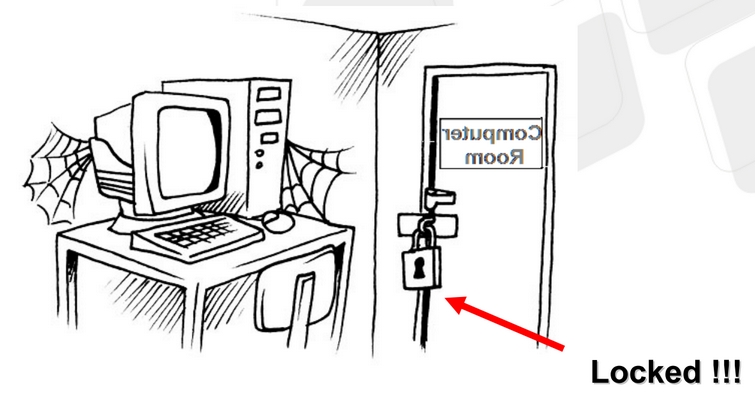
\includegraphics[max size={\textwidth}{\textheight}]{../../imagens/computer-room.png}

	\end{center}

	\caption{\label{5817b264c8a300b4b46214039b2e579aba5d70a7}Arte produzida sob encomenda para a avalia\c{c}\~ao do OLPC, expondo a situa\c{c}\~ao dos laborat\'orios de micro-computadores de muitas escolas brasileiras no final de s\'eculo XX, in\'{i}cio do XXI. (Fonte: acervo pessoal de Victor Mammana)}

\end{figure}

A avalia\c{c}\~ao do Governo Brasileiro j\'a percebia que o OLPC exagerava o papel que uma simples ferramenta digital (laptop) poderia desempenhar no processo educacional, mas reconhecia que o uso desta ferramenta na escola poderia \textquotedbl permitir uma melhor prepara\c{c}\~ao para a sobreviv\^encia do educando na sociedade de informa\c{c}\~ao, criando oportunidades para sua inclus\~ao como membro ativo desta sociedade\textquotedbl .










Mas o programa tamb\'em criava muita inseguran\c{c}a nas autoridades brasileiras e a partir de agora citamos algumas, com base nos achados descritos por MAMMANA (2006) em seu relat\'orio final de avalia\c{c}\~ao, concentrando-nos em quest\~oes de cunho estrat\'egico e geopol\'{\i}tico:











\begin{alineas}
\item \textquotedbl Em \'ultima an\'alise, o OLPC \'e um projeto de poder, com m\'eritos e agendas alternativas \`as dos Estados Nacionais, que atua na \'area mais sens\'{\i}vel de qualquer sociedade: sua reprodu\c{c}\~ao e reinven\c{c}\~ao, ou seja, a educa\c{c}\~ao.\textquotedbl 
\item \textquotedbl A ades\~ao ao OLPC coloca a internet no centro do processo de aprendizagem, promovendo a converg\^encia final entre educa\c{c}\~ao e m\'{\i}dia.\textquotedbl 
\item \textquotedbl A despeito de qualquer paran\'oia, a previs\~ao de qual \'e a dire\c{c}\~ao e evolu\c{c}\~ao do controle da internet \'e objeto de muita controv\'ersia em todos os meios, mas deve ser tema de reflex\~ao por parte das autoridades que decidir\~ao pela ades\~ao ao OLPC, pela relev\^ancia que a mesma assume no contexto do programa.\textquotedbl 
\item \textquotedbl O que deve ser evitado pelo governo brasileiro \'e a ades\~ao extempor\^anea a um programa cuja a agenda \'e controlada por grupos que n\~ao est\~ao sob a esfera de influ\^encia do poder democr\'atico institu\'{\i}do em nosso pa\'{\i}s\textquotedbl 
\item \textquotedbl Mais do que a converg\^encia de tecnologias de informa\c{c}\~ao e comunica\c{c}\~ao (TICs), a proposta OLPC tr\'as em si a converg\^encia da m\'{\i}dia com a educa\c{c}\~ao, quando esta \'ultima passa a ser, definitivamente (e pela aus\^encia de uma vis\~ao de cidadania associada), dominada por agentes econ\^omicos globais que custodiam e controlam os conte\'udos que at\'e agora t\^em sido oferecidos democraticamente pela sociedade aos seus reposit\'orios.\textquotedbl 
\item \textquotedbl Atrav\'es de uma intensa atividade de persuas\~ao nas estruturas de poder de v\'arios pa\'{\i}ses, os representantes da Organiza\c{c}\~ao OLPC, que em parte s\~ao oriundos do Media Lab, v\^em buscando a ades\~ao de diversos governos do mundo para um programa de ado\c{c}\~ao de laptops de baixo custo nas atividades curriculares de suas redes de ensino fundamental e m\'edio. Simultaneamente a esta atividade com os governos, \'e razo\'avel acreditar que a Organiza\c{c}\~ao OLPC est\'a, tamb\'em, estabelecendo contratos e acordos que n\~ao t\^em sido divulgados ao p\'ublico e a estes governos. Uma das justificativas para esta n\~ao divulga\c{c}\~ao pode ser a preocupa\c{c}\~ao com for\c{c}as antag\^onicas da ind\'ustria, as quais, por terem seu mercado amea\c{c}ado, podem se utilizar destas informa\c{c}\~oes estrat\'egicas para reagir \`a implementa\c{c}\~ao do OLPC.\textquotedbl 
\item \textquotedbl A proposta OLPC \'e parcialmente financiada por agentes que a imprensa frequentemente associa ao universo de think tanks conservadores e ONGs com interesse geopol\'{\i}tico [1], al\'em de empresas de M\'{\i}dia com poss\'{\i}vel interesse no acesso a novos mercados, como \'e o caso da Google.\textquotedbl 
\item \textquotedbl Subjacente a vis\~ao do OLPC est\'a a viabiliza\c{c}\~ao do acesso irrestrito a informa\c{c}\~oes que, se por um lado hoje t\^em diversidade impressionante e acredita-se, est\~ao dispon\'{\i}veis de forma democr\'atica na internet, por outro lado est\~ao sob cust\'odia e escrut\'{\i}nio de estruturas de dissemina\c{c}\~ao de informa\c{c}\~ao dominadas por empresas privadas globais, num modelo de governan\c{c}a da internet que atribui a um \'unico Estado Hegem\^onico o poder discricion\'ario sobre toda a rede (ICANN).\textquotedbl 
\end{alineas}

Os pontos levantados pela avalia\c{c}\~ao do OLPC por parte de pesquisadores brasileiros levaram a um alerta seguido de uma recomenda\c{c}\~ao:











\noindent\begin{center}\mbox{\centering\fbox{\centering\par\parbox{0.7\linewidth}{\small\textit{\textquotedbl (...) Neste contexto, deve ser evitada a ades\~ao extempor\^anea a um programa cuja a agenda \'e controlada por grupos que n\~ao est\~ao sob a esfera de influ\^encia do poder democr\'atico institu\'{\i}do em nosso pa\'{\i}s. (...) A impossibilidade de prever o que pode acontecer e a certeza de que existem consequ\^encias para o modelo de democracia brasileiro, devem ser o pano de fundo para a tomada de decis\~ao sobre o que fazer com o OLPC. Embora nenhuma a\c{c}\~ao nesta dire\c{c}\~ao tenha sido tomada, sabe-se que h\'a como enquadrar o OLPC naquilo que a sociedade considerar mais conveniente para a cidadania do brasileiro.\textquotedbl  (Fonte:  MAMMANA (2006))}\normalsize}}}\end{center}


Percebe-se, no posicionamento acima, uma preocupa\c{c}\~ao com a possibilidade de forma\c{c}\~ao de estruturas de dissemina\c{c}\~ao de informa\c{c}\~ao em que os valores da cidadania poderiam deixar de ser preponderantes. Em parte, pode-se dizer que as redes sociais de hoje est\~ao se prestando a esse servi\c{c}o, transformando-se me meios para a dissemina\c{c}\~ao de informa\c{c}\~oes falsas, crimes, entre outros. Interpretando a posteriori, e por meio de comunica\c{c}\~ao privada recente do autor da avalia\c{c}\~ao, parece-nos que o posicionamento do CTI se insurgia contra a subordina\c{c}\~ao da escola brasileira, ber\c{c}o de nossa cidadania, a esse poder monumental.










Dentre as atividades atribu\'{\i}das a Victor Mammana no per\'{\i}odo de avalia\c{c}\~ao do OLPC, estava o acompanhamento do desenvolvimento do laptop em si, aproveitando a experi\^encia do mesmo com pol\'{\i}tica industrial na \'area de mostradores de informa\c{c}\~oes (displays) para avaliar a viabilidade tecnol\'ogica das solu\c{c}\~oes propostas. A figura XXX mostra uma foto emblem\'atica da situa\c{c}\~ao do desenvolvimento do OLPC, que gerava muita inseguran\c{c}a no Governo Brasileiro. Na foto, tirada por Victor Mammana, \'e poss\'{\i}vel ver que o \textquotedbl prot\'otipo\textquotedbl  apresentado a Kofi Anan n\~ao tinha \textquotedbl placa m\~ae\textquotedbl  e n\~ao era um produto real. A placa m\~ae estava embaixo da mesa. Um extenso relat\'orio foi apresentado ao Coordenador da For\c{c}a Tarefa Brasileira de avalia\c{c}\~ao do OLPC, Dr. C\'esar Alvarez, gerando questionamentos \`a equipe do OLPC sobre o real est\'agio de desenvolvimento do prot\'otipo do dito \textquotedbl laptop de 100 d\'olares\textquotedbl   (MAMMANA, 2005).












\captionsetup{format=plain}
\begin{figure}[htb]

	\begin{center}

		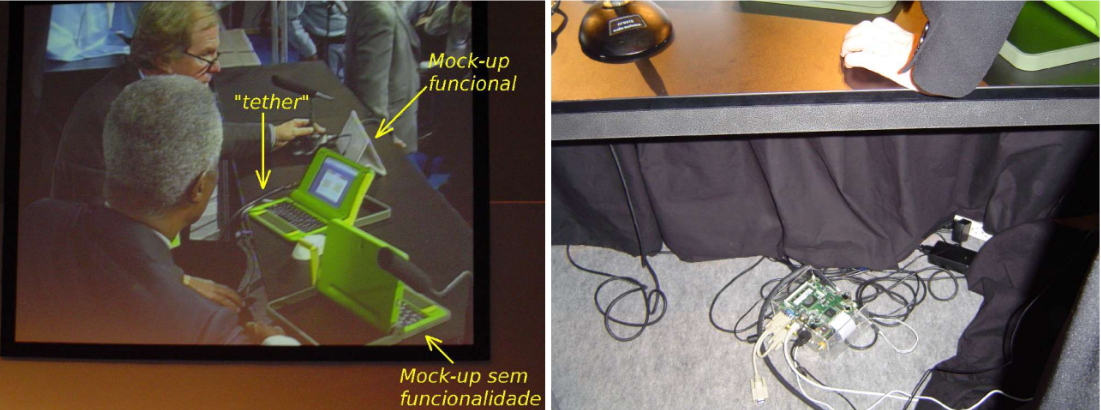
\includegraphics[max size={\textwidth}{\textheight}]{../../imagens/embaixo-mesa.png}

	\end{center}

	\caption{\label{009ca00e74581d7c5448a43112358cb91a959b69}Foto tirada por Victor Mammana mostrando que o OLPC ainda n\~ao tinha um prot\'otipo completo, mesmo com as negocia\c{c}\~oes avan\c{c}adas com o Governo Brasileiro. Essa situa\c{c}\~ao gerou muita inseguran\c{c}a na Presid\^encia da Rep\'ublica. (cr\'editos: Victor Mammana)}

\end{figure}

Sobre essa situa\c{c}\~ao,  MAMMANA (2006) alerta:











\noindent\begin{center}\mbox{\centering\fbox{\centering\par\parbox{0.7\linewidth}{\small\textit{\textquotedbl Do ponto de vista t\'ecnico \'e preciso estar atento \`as cr\'{\i}ticas referentes \`a maneira desestruturada com que v\^em sendo proposto, gerando preocupa\c{c}\~oes sobre sua viabilidade pedag\'ogica, industrial, financeira e social, no longo prazo.\textquotedbl  (Fonte:  MAMMANA (2006))}\normalsize}}}\end{center}


Outro aspecto analisado foi a ergonomia, tendo sido constatado que laptops s\~ao intrinsecamente n\~ao ergon\^omicos, por vincular a tela ao teclado numa mesma \textquotedbl caixa\textquotedbl . Quando a tela est\'a numa posi\c{c}\~ao adequada para os olhos, o teclado fica em posi\c{c}\~ao inadequada, e vice-versa  (HIRAGA et al., 2006).










Sobre isso,  HIRAGA et al. (2006) constata:











\noindent\begin{center}\mbox{\centering\fbox{\centering\par\parbox{0.7\linewidth}{\small\textit{\textquotedbl Ficou evidente que o programa OLPC n\~ao leva em conta aspectos importantes de ergonomia quanto ao uso saud\'avel do laptop, como por exemplo, a postura corporal do usu\'ario, o tempo de uso, o mobili\'ario a ser utilizado, entre outros.\textquotedbl  (Fonte:  HIRAGA et al. (2006))}\normalsize}}}\end{center}


Ao longo das an\'alises presentes nas dezenas de relat\'orios de avalia\c{c}\~ao gerados, muitas outras quest\~oes geraram questionamentos cuja resposta n\~ao parecia satisfat\'oria, a exemplo de:











\begin{alineas}
\item obsolesc\^encia dos equipamentos e descarte seguro de lixo-eletr\^onico
\item custo de aquisi\c{c}\~ao para o governo brasileiro
\item manuten\c{c}\~ao dos equipamentos
\item garantia de acesso \`a internet no prazo necess\'ario
\item seguran\c{c}a das crian\c{c}as em v\'arios aspectos (e.g. conte\'udos impr\'oprios, exposi\c{c}\~ao a situa\c{c}\~oes de risco nas redes sociais)
\item capacita\c{c}\~ao dos profissionais de educa\c{c}\~ao para promover a melhor utiliza\c{c}\~ao dos equipamentos
\item custo da infraestrutura perif\'erica (adequa\c{c}\~ao do mobili\'ario, sistemas de carregamento de baterias, entre outros)
\end{alineas}

Em suma, o que se constatou \'e que, pelas dimens\~oes do Brasil e os prazos ex\'{\i}guos de ades\~ao exigidos pelo OLPC, havia muitos riscos para o sistema educacional brasileiro. Por outro lado, para pa\'{\i}ses menores, a ades\~ao poderia fazer mais sentido, dado que essas quest\~oes poderiam ser tratadas com mais detalhe e controle.










N\~ao obstante todas estas d\'uvidas, o valor da proposta OLPC foi reconhecido. \'E poss\'{\i}vel identificar na documenta\c{c}\~ao existente a \^ansia dos pesquisadores envolvidos em encontrar uma alternativa que fosse mais adequada \`a realidade brasileira, mas que, ao mesmo tempo, permanecesse usufruindo das virtudes pedag\'ogicas da proposta de Papert, sem os desafios or\c{c}ament\'arios, industriais e log\'{\i}sticos da forma de implanta\c{c}\~ao decorrente da proposta de Negroponte.










Um outro elemento importante para a concep\c{c}\~ao do WASH foi a avalia\c{c}\~ao do Programa de Inclus\~ao Digital (PID) do Minist\'erio da Ci\^encia e Tecnologia (MCT), que era conduzido pela Secretaria de Inclus\~ao Social nos anos de 2005 a 2009.










O PID do Minist\'erio da Ci\^encia e Tecnologia (MCT) na primeira d\'ecada do s\'eculo era fundamentado na disponibiliza\c{c}\~ao de infraestrutura, na forma de telecentros, carecendo de uma vis\~ao mais estruturada e sem previs\~ao de investimento nos verdadeiros atores do processo: as pessoas (CGEE, 2010). A maior parte do investimento era voltada para constru\c{c}\~ao de edifica\c{c}\~oes e aquisi\c{c}\~ao de equipamentos.










A avalia\c{c}\~ao do PID tamb\'em ficou a cargo do Dr. Victor Mammana, atrav\'es de um contrato com o Centro de Gest\~ao e Estudos Estrat\'egicos do MCT. Pudemos constatar que esse trabalho de avalia\c{c}\~ao foi o grande marco para a concep\c{c}\~ao do WASH, de onde surgem alguns elementos que hoje est\~ao presentes na Portaria CTI 178/2018 aparecem pela primeira vez.










O PID era um programa baseado em recursos oriundos de emendas parlamentares, direcionadas para disseminar telecentros por todo o pa\'{\i}s. Os recursos eram repassados para a SECIS, que gerenciava a cria\c{c}\~ao dos telecentros nas cidades interessadas, com apoio t\'ecnico da Caixa Econ\^omica. Cerca de 150 milh\~oes de reais foram empregados em 5 anos, em projetos de inclus\~ao social e digital (CGEE, 2010), colocando a iniciativa em patamar equivalente ao do Pro-Info para o mesmo per\'{\i}odo. O formato era particularmente atraente para os parlamentares, que podiam destinar o investimento para suas bases eleitorais. Isso inaugurou um inusitado interesse dos parlamentares pelo MCT.










Os telecentros, no contexto do PID, eram estruturas f\'{\i}sicas (pr\'edios) equipados com computadores e conectividade (muitas vezes viabilizada pelo GESAC), com vistas a oferecer acesso \`a internet para os cidad\~aos da regi\~ao. Sobre isso, CGEE (2010) sintetiza o tipo de equipamento p\'ublico que se pretendia construir no contexto do PID, antes de 2008:











\noindent\begin{center}\mbox{\centering\fbox{\centering\par\parbox{0.7\linewidth}{\small\textit{\textquotedbl (...) edifica\c{c}\~ao sob mando de uma institui\c{c}\~ao local, edifica\c{c}\~ao esta que, oficialmente: pode sofrer reformas, receber computadores conectados \`a internet, devendo estar aberta ao p\'ublico e oferecer acessibilidade f\'{\i}sica. A edifica\c{c}\~ao pode conter corpo de apoio, que por sua vez pode receber uma \'unica rodada de capacita\c{c}\~ao\textquotedbl  (Fonte: CGEE (2010))}\normalsize}}}\end{center}


Esta descri\c{c}\~ao, por si s\'o, mostra muitas fragilidades do Programa PID na sua concep\c{c}\~ao original, porque:











\noindent\begin{center}\mbox{\centering\fbox{\centering\par\parbox{0.7\linewidth}{\small\textit{\textquotedbl o resultado pretendido se omite quando n\~ao orienta o gestor local sobre op\c{c}\~oes de arranjo institucional para o centro/unidade, quando n\~ao prepara o sistema para a avalia\c{c}\~ao continuada, quando tangencia a quest\~ao educacional e se satisfaz com uma rela\c{c}\~ao com a municipalidade limitada ao tempo de implanta\c{c}\~ao do projeto, sem criar mecanismos para perpetuar esta intera\c{c}\~ao\textquotedbl  (Fonte: CGEE (2010))}\normalsize}}}\end{center}


Foi da an\'alise das defici\^encias do OLPC e do PID, com influ\^encias do trabalho de Afira Ripper, que o Programa WASH nasceu, com ideias cujo amadurecimento se consolidou em 2009-2010, quando o relat\'orio final de avalia\c{c}\~ao do PID foi entregue  (CGEE, 2010). Naquele relat\'orio apresentado ao CGEE surge, na forma de recomenda\c{c}\~ao para a revis\~ao do PID, os elementos que depois seriam a base do WASH, registrados tamb\'em na Portaria CTI 178/2018. Textualmente, consta o seguinte em  CGEE (2010):











\noindent\begin{center}\mbox{\centering\fbox{\centering\par\parbox{0.7\linewidth}{\small\textit{\textquotedbl A SECIS poderia, em conjunto com o CNPq, criar bolsas semelhantes \`as existentes para promo\c{c}\~ao da excel\^encia da doc\^encia (e.g. PQ e DT), mas no caso voltadas para motivar a participa\c{c}\~ao \`a dist\^ancia de membros da academia nos projetos do PIDS. Esta participa\c{c}\~ao poderia se dar de diversas formas, como por exemplo pela orienta\c{c}\~ao de alunos de inicia\c{c}\~ao cient\'{\i}fica atuantes dentro dos centros/unidades, ou mesmo pela verifica\c{c}\~ao dos procedimentos pedag\'ogicos, proposi\c{c}\~ao de melhorias, elabora\c{c}\~ao de relat\'orios, verifica\c{c}\~ao de resultados, etc. Este membro da academia, com caracter\'{\i}sticas de um “tutor”, se transformaria num agente da SECIS e elo entre ela e a “ponta”. A atua\c{c}\~ao deste agente poderia se dar no contexto de suas atividades acad\^emicas, dentro da universidade em que estivesse sediado.\textquotedbl  (Fonte:  CGEE (2010))}\normalsize}}}\end{center}


O texto acima foi produzido 4 anos antes do primeiro evento do WASH (2013), antecipando parcialmente as caracter\'{\i}sticas que posteriormente estariam presentes na Portaria CTI 178/2018, quase uma d\'ecada depois. Este registro mostra que a proposta do WASH tem base num aprendizado muito longo sobre pol\'{\i}ticas p\'ublicas de educa\c{c}\~ao (OLPC), de inclus\~ao (PID) e de governo eletr\^onico (GESAC), embasando-se em fontes seguras e robustas.










\subsection[Papert no Brasil pela \'otica de Afira Ripper]{Papert no Brasil pela \'otica de Afira Ripper}\label{Papert no Brasil pela \'otica de Afira Ripper}
Nesta se\c{c}\~ao trazemos uma vis\~ao sobre como Papert se aproximou do Brasil na d\'ecada de 70, a qual nem sempre est\'a presente na literatura sobre o assunto. Para isso, usamos como fonte a entrevista da Profa. Dra. Afira Vianna Ripper, que foi testemunha ocular do que aconteceu naquele per\'{\i}odo. Sua entrevista \'e um dos produtos de nossa disserta\c{c}\~ao, uma vez que, com a contribui\c{c}\~ao de Angel Lu\'{\i}s e Will Namen, um esmerado trabalho de edi\c{c}\~ao foi realizado para garantir uma boa qualidade e longevidade do material. Esta entrevista consta na se\c{c}\~ao de Produtos Tecnol\'ogicos desta disserta\c{c}\~ao, uma vez que foi empenhado um esfor\c{c}o tecnol\'ogico para garantir sua acessibilidade.










Professora da Pedagogia da Unicamp desde a d\'ecada de 70, atualmente aposentada, Afira \'e uma figura que esteve presente em v\'arios momentos impactantes para a hist\'oria que se registra aqui. Sobressai o papel pioneiro que  desempenhou na cidade de Campinas na d\'ecada de 90, quando levou, em car\'ater piloto, pr\'aticas de Papert para escolas p\'ublicas municipais. Ela inaugurou o emprego de Bolsas da FAPESP (Funda\c{c}\~ao Paulista equivalente ao CNPq) direcionadas a professores do fundamental participantes do projeto, uma abordagem que guarda certa similitude com o que foi implementado no WASH, no caso de Bolsas de Extens\~ao do CNPq. O Coordenador do WASH, em comunica\c{c}\~ao privada feita diretamente para esta candidata, reconhece a influ\^encia desse projeto na concep\c{c}\~ao do WASH.










Outro momento em que as hist\'orias se cruzaram foi a participa\c{c}\~ao de Afira Ripper na avalia\c{c}\~ao do OLPC em 2006, convidada pelo atual coordenador do WASH, que na \'epoca coordenava a avalia\c{c}\~ao por parte do CTI. Naquele epis\'odio, segundo relato do coordenador do WASH, reencontrou muitos daqueles que interagira no MIT, a exemplo de David Cavallo, entre outros. Ali\'as, seu esposo esteve presente em atividades do Centre Mondial Informatique et Ressource Humaine, na d\'ecada de 80, onde Negroponte atuou como Diretor.










Como se v\^e, Afira foi uma observadora brasileira privilegiada no que se refere \`as contribui\c{c}\~oes de Papert, e n\~ao \'e exagero dizer que a chegada precoce da \textquotedbl filosofia\textquotedbl  LOGO no Brasil teve grande contribui\c{c}\~ao dela.










Afira havia se transferido para os Estados Unidos no come\c{c}o da d\'ecada de 60 para acompanhar seu esposo, o Prof. Jos\'e Ellis Ripper Filho, em seu doutorado no MIT.










Inquieta e comprometida com sua carreira, n\~ao era seu perfil permanecer apenas como acompanhante do esposo e buscou uma atividade no seu campo de forma\c{c}\~ao. Foi assim que se engajou como aluna ouvinte no MIT, tendo sido estudante e depois convivido profissionalmente com Papert, em 1973. A experi\^encia foi bastante marcante para ela, tendo impacto tamb\'em na sua vida pessoal, dado que seu filho foi a primeira crian\c{c}a brasileira a experimentar o LOGO, quando estava sendo instalado o Media Lab no MIT.










A Professora Afira retornou ao Brasil e foi trabalhar num projeto de matem\'atica junto com o Professor Ubiratan D’ambr\'osio, Diretor do Instituto de matem\'atica da Unicamp, IMEC. A experi\^encia de Afira no grupo de Papert motivou um convite para que Seymour Papert, da \'area de educa\c{c}\~ao, e Marvin Minsky, da \'area de intelig\^encia artificial, viessem ao Brasil.










Antes de prosseguir, \'e preciso abrir um par\^enteses sobre como a Profa. Afira Ripper optou pela Unicamp, em seu retorno ao Brasil.  MAMMANA (2018), ap\'os entrevista com Prof. Jos\'e Ellis Ripper Filho, esposo da Profa. Afira, traz um relato interessante sobre a decis\~ao dos pesquisadores brasileiros, expatriados nos Estados Unidos na d\'ecada de 60, de retornarem ao Brasil em plena ditadura. Em resumo, a escolha de Campinas foi decorrente da invas\~ao da UNB pelo Ex\'ercito em 1968. Bras\'{\i}lia era o destino preferido dos pesquisadores Brasileiros, por conta da proposta arrojada de Darcy Ribeiro para a UNB, mas ponderaram o risco de estarem pr\'oximos demais da \textquotedbl toca do le\~ao\textquotedbl   (MAMMANA, 2018), optando pela Unicamp. Essa decis\~ao dos pesquisadores foi determinante para a consolida\c{c}\~ao da UNICAMP e, consequentemente, para a voca\c{c}\~ao de Campinas em ci\^encia e tecnologia que se observou nas d\'ecadas subsequentes.










Cabe registrar que o papel de Ubiratan D Ambr\'osio \'e relatado tamb\'em por ALVAREZ (2015), mas a nuance do papel da Profa. Afira Ripper n\~ao \'e relatada.










Ali\'as, h\'a ainda que se uniformizar as fontes hist\'oricas para identificar o papel de cada institui\c{c}\~ao brasileira nesse per\'{\i}odo. Por exemplo,  ALVAREZ (2015) menciona o pioneirismo da Universidade Federal do Rio de Janeiro, 1966, no uso de computador em atividades acad\^emicas. Por outro lado, o ITA reinvindica a constru\c{c}\~ao do primeiro computador em 1963, constru\'{\i}do no contexto de um curso de gradua\c{c}\~ao, com a participa\c{c}\~ao do ent\~ao estudante Jos\'e Ripper Ellis Ripper.










Naquele tempo, d\'ecada de 70, a intelig\^encia artificial era uma disciplina extremamente nova. Os pesquisadores do MIT vieram para passar um m\^es dando palestras no IMEC da UNICAMP sobre o programa de intelig\^encia artificial e o programa do LOGO, que ainda estava numa fase inicial mesmo nos Estados Unidos. Afira relata que a primeira medida tomada pelos professores da Unicamp foi traduzir o livro do Papert sobre a linguagem LOGO.










Os professores brasileiros j\'a estavam contaminados pela ideia de que o trabalho com o computador poderia empoderar as crian\c{c}as em rela\c{c}\~ao ao exerc\'{\i}cio dos racioc\'{\i}nios matem\'atico e l\'ogico. \textquotedbl Refiro-me ao computador do pr\'e mouse, um computador em que voc\^e digitava os comandos e tinha que apertar o enter\textquotedbl , diz Afira Ripper sobre a interface de computador existente naquele tempo.










Muitos desenvolvimentos se seguiram depois, at\'e o ponto em que a Profa. Afira Ripper percebeu-se em condi\c{c}\~oes de estabelecer um projeto semelhante ao do MIT no Brasil.










Afira formulou o Projeto Eureka, que pretendia introduzir o computador na escola como ferramenta pedag\'ogica para o trabalho do professor. O Projeto foi apresentado para a Secretaria Municipal de Educa\c{c}\~ao de Campinas, tendo sido aceito como projeto pedag\'ogico no \^ambito da secretaria.










Ainda segundo o relato da Profa. Afira Ripper, posteriormente uma diretora de pr\'e-escola (p\'ublica) de Campinas abarcou o projeto de pesquisa e inicia\c{c}\~ao cient\'{\i}fica, formando as professoras que passariam a trabalhar com os alunos, dentro da filosofia de Montessori. Na interpreta\c{c}\~ao da Profa. Afira, esta abordagem criava uma responsabilidade redobrada para os alunos que, motivados pelo LOGO, fazia com que eles tivessem um interesse enorme pelo computador, mesmo com barreiras iniciais, como a digita\c{c}\~ao, por exemplo.










Em sua entrevista, a Afira reporta um impressionante interesse pelo que eles pr\'oprios conseguiam fazer no computador. Ainda, segundo sua descri\c{c}\~ao, as crian\c{c}as digitavam os c\'odigos e as professoras pediam para que fizessem os gestos dos comandos do LOGO: \textquotedbl em p\'e\textquotedbl , \textquotedbl vire \`a direita\textquotedbl , \textquotedbl vire \`a esquerda\textquotedbl , \textquotedbl d\^e passos para frente\textquotedbl , \textquotedbl para tr\'as\textquotedbl . Tanto para as crian\c{c}as quanto para os adultos, era um in\'{\i}cio da computa\c{c}\~ao em suas vidas.










Assim, foi poss\'{\i}vel trazer o LOGO como um elemento a mais para levar ao exerc\'{\i}cio natural de conceitos da l\'ogica, da \'algebra, das fun\c{c}\~oes e da teoria de conjuntos, criando um passo-a-passo menos traum\'atico para se chegar a uma experi\^encia mais org\^anica em torno da matem\'atica. Ao mesmo tempo, o LOGO n\~ao se restringe \`a superf\'{\i}cie dos conceitos, permitindo que o pensamento humano experimente ideias bem mais complexas e abstratas, como por exemplo a ideia da recurs\~ao, em que algoritmos invocam a si mesmos at\'e os limites da mem\'oria do computador.










Outra pesquisadora do LOGO, no Brasil, foi a professora Maria Cec\'{\i}lia Baranauskas (Unicamp), que investigou como a intera\c{c}\~ao de crian\c{c}as com o computador se dava, utilizando a Linguagem LOGO em um terminal gr\'afico (GT40), ligado a um mainframe (PDP10), do Centro de Computa\c{c}\~ao da UNICAMP. A sua disserta\c{c}\~ao de Mestrado foi sobre os \textquotedbl Conceitos Geom\'etricos, atrav\'es da Linguagem LOGO\textquotedbl . O Programa WASH publicou entrevista com a professora Maria Cec\'{\i}lia Baranauskas [XXX], na qual ela conta a sua experi\^encia com a Linguagem LOGO e rememora o seu contato com Papert e sua teoria. A entrevista est\'a dispon\'{\i}vel neste link: \textquotedbl Barreiras entre o homem e o computador e oficinas digitais s\~ao temas com membro da Unesco, Programa Wash\textquotedbl .










\subsection[Os valores e conceitos do Programa WASH]{Os valores e conceitos do Programa WASH}\label{Os valores e conceitos do Programa WASH}
Nesta se\c{c}\~ao fazemos uma interpreta\c{c}\~ao do acervo de documentos do Programa WASH, principalmente os relat\'orios apresentados ao CNPq durante os anos de execu\c{c}\~ao de seus projetos intermedi\'arios, visando identificar os valores e conceitos gerais do Programa WASH. Veja que n\~ao trataremos nesta se\c{c}\~ao de descrever o funcionamento do Projeto WASH, em termos de seus processos, assunto que ser\'a tratado no \^ambito do eixo 2 desta disserta\c{c}\~ao.










Segundo MAMMANA et al. (2020), o Programa WASH foi iniciado em 28 de setembro de 2013 com um \textquotedbl \'unico e pontual evento de hackers\textquotedbl . O foco em \textquotedbl hackers\textquotedbl  indica que o p\'ublico alvo, inicial, era constitu\'{\i}do de jovens em adultos.










Esse fato por si s\'o indica que, a rigor, a organiza\c{c}\~ao do primeiro evento n\~ao vislumbrava a incorpora\c{c}\~ao das ideias preconizadas na avalia\c{c}\~ao do PID  (CGEE, 2010).










O caminho em dire\c{c}\~ao a um programa educacional como o anteciopado pela avalia\c{c}\~ao do PID foi sendo moldado ao longo de suas re-edi\c{c}\~oes, que gradualmente passaram a atrair um p\'ublico cada vez mais jovem, culminando no encontro definitivo de sua voca\c{c}\~ao, j\'a em 2014:











\noindent\begin{center}\mbox{\centering\fbox{\centering\par\parbox{0.7\linewidth}{\small\textit{\textquotedbl educa\c{c}\~ao cient\'{\i}fica e tecnol\'ogica para o ensino fundamental, mediante protagonismo de jovens do ensino m\'edio e superior\textquotedbl  (Fonte:  MAMMANA et al. (2020))}\normalsize}}}\end{center}


Ambicionando aplicar o que fora aprendido com avalia\c{c}\~ao pedag\'ogica do OLPC, inclusive com a influ\^encia e colabora\c{c}\~ao de Afira Ripper, o WASH sempre buscou se vincular aos conceitos subjacentes ao pensamento de Papert.










Rapidamente, acompanhando a tend\^encia mundial, o programa se identificou com o STEM (Science, Technology, Engineering and Mathematics), adotando tamb\'em as artes como um elemento fundamental de suas oficinas  (MAMMANA et al., 2020). Posteriormente, mas independentemente dos conceitos constru\'{\i}dos por outros (e.g.  YAKMAN (2019)), esta candidata prop\^os a introdu\c{c}\~ao das artes nas oficinas do WASH, aproximando-a das abordagens STEAM.










Essa mudan\c{c}a de \textquotedbl evento de hackers\textquotedbl  para \textquotedbl evento STEAM\textquotedbl  exigiu um compromisso maior com o conceito de m\'etodo cient\'{\i}fico, requerendo do programa a ado\c{c}\~ao de um \textquotedbl crit\'erio de demarca\c{c}\~ao\textquotedbl  da ci\^encia.










 CHIBENI (2006) alerta para o fato de que \textquotedbl n\~ao h\'a um m\'etodo cient\'{\i}fico no sentido de uma receita universal para se fazer ci\^encia\textquotedbl , mas \'e poss\'{\i}vel identificar na ci\^encia algumas especificidades em rela\c{c}\~ao a outras formas de adquirir saber.










Os criadores do WASH, em v\'arios pontos da documenta\c{c}\~ao existente, mencionam inicialmente o crit\'erio da falseabilidade de Popper como forma de verificar se uma proposi\c{c}\~ao \'e cient\'{\i}fica ou n\~ao e, portanto, pass\'{\i}vel de fazer parte das atividades do programa. Para isso, apresentam a seguinte defini\c{c}\~ao como sendo uma \textquotedbl forma simplificada de expressar o pensamento de Popper\textquotedbl   (MAMMANA et al., 2020):











\noindent\begin{center}\mbox{\centering\fbox{\centering\par\parbox{0.7\linewidth}{\small\textit{Falseabilidade - Todo conhecimento cient\'{\i}fico pode ser questionado e contestado, quando pode ser requerida a revis\~ao de suas bases experimentais e te\'oricas. O conhecimento que n\~ao pode ser contestado, a exemplo da f\'e religiosa ou do ocultismo, n\~ao \'e um conhecimento cient\'{\i}fico.}\normalsize}}}\end{center}


\'E poss\'{\i}vel identificar na documenta\c{c}\~ao do WASH o reconhecimento de que o crit\'erio da falseabilidade foi considerado como um \textquotedbl ponto de partida\textquotedbl  para o trabalho de \textquotedbl demarca\c{c}\~ao de ci\^encia e n\~ao-ci\^encia\textquotedbl , mas que para \textquotedbl os primeiros anos escolares \'e preciso resistir \`a tenta\c{c}\~ao de ir muito al\'em disso na busca por uma defini\c{c}\~ao \'unica e generalizada do m\'etodo cient\'{\i}fico\textquotedbl   (MAMMANA et al., 2020).










O que se identifica nas pr\'aticas do WASH, seja pela inspe\c{c}\~ao da documenta\c{c}\~ao formal (relat\'orios), quanto pela busca dos temas de oficinas na plataforma \textquotedbl Platu\'oxe\textquotedbl , \'e que n\~ao h\'a uma preocupa\c{c}\~ao em definir o m\'etodo cient\'{\i}fico para as crian\c{c}as, adotando como \textquotedbl divisa\textquotedbl  a ideia simples de que \textquotedbl se voc\^e pode questionar, \'e ci\^encia\textquotedbl   (MAMMANA et al., 2020). Esta simplifica\c{c}\~ao est\'a de bom tamanho para os anos escolares iniciais, mas \'e claro que precisa se ampliar, com o amadurecimento.










A intera\c{c}\~ao com o coordenador do Programa WASH, bem como a an\'alise da documenta\c{c}\~ao existente  (MAMMANA et al., 2020)  (MAMMANA et al., 2020a)  (MAMMANA et al., 2022a) , mostra que existe uma predile\c{c}\~ao por uma defini\c{c}\~ao bastante simples e direta de ci\^encia, que \'e de f\'acil assimila\c{c}\~ao por todos os colaboradores:











\noindent\begin{center}\mbox{\centering\fbox{\centering\par\parbox{0.7\linewidth}{\small\textit{\textquotedbl Ci\^encia \'e a compreens\~ao que o outro constr\'oi sobre o conhecimento de algu\'em\textquotedbl  (Fonte:  CGEE (2010), p\'ag. 48)}\normalsize}}}\end{center}


A frase acima foi primeiramente apresentada em  CGEE (2010) pelo coordenador do projeto, tendo car\'ater original. O conceito subjacente \'e de que \textquotedbl n\~ao h\'a ci\^encia se n\~ao houver a compreens\~ao por algu\'em dos conhecimentos gerados por outrem, mostrando que a ci\^encia tem car\'ater social, sendo parte integrante da cultura de uma comunidade\textquotedbl   (MAMMANA et al., 2020).










A forma como esse conceito \'e aproveitado no contexto da escola fundamental fica evidente na transcri\c{c}\~ao de MAMMANA et al. (2020) apresentada abaixo:











\noindent\begin{center}\mbox{\centering\fbox{\centering\par\parbox{0.7\linewidth}{\small\textit{\textquotedbl Na atua\c{c}\~ao do WASH junto aos primeiros anos escolares, h\'a uma preocupa\c{c}\~ao de estimular uma boa comunica\c{c}\~ao, seja atrav\'es da prepara\c{c}\~ao dos bolsistas para a multiplica\c{c}\~ao (oficinas), registro de resultados ou prepara\c{c}\~ao de audio-visuais, por exemplo. Em outras palavras, \'e a preocupa\c{c}\~ao com a capacidade de produzir narrativas calcadas num m\'etodo.\textquotedbl  (Fonte:  MAMMANA et al. (2020))}\normalsize}}}\end{center}


Este est\'{\i}mulo \`a produ\c{c}\~ao de narrativas que facilitem a compreens\~ao de algum conhecimento \'e, em \'ultima an\'alise, o m\'etodo cient\'{\i}fico do WASH. Atrav\'es dele, a crian\c{c}a ou jovem \'e convidado a organizar o conhecimento adquirido para que, atrav\'es da convers\~ao em um discurso, outro possa assimil\'a-lo e question\'a-lo. Esta abordagem fica bem clara em  WASHCNPq (2022):











\noindent\begin{center}\mbox{\centering\fbox{\centering\par\parbox{0.7\linewidth}{\small\textit{\textquotedbl (...) Outra atividade oferecida pelo WASH \'e a constru\c{c}\~ao de discursos pelos participantes, muitas vezes na dire\c{c}\~ao de uma produ\c{c}\~ao audiovisual como ferramenta para o exerc\'{\i}cio de comunica\c{c}\~ao de suas descobertas e aprendizados. Nesse processo, s\~ao estimulados o planejamento, o debate de ideias, o trabalho em coopera\c{c}\~ao, a organiza\c{c}\~ao e algumas t\'ecnicas de produ\c{c}\~ao audiovisual, embora este \'ultimo aspecto seja mais instrumental. Tudo isso \'e feito de forma l\'udica e dentro da zona proximal da crian\c{c}a.\textquotedbl  (Fonte: W WASHCNPq (2022))}\normalsize}}}\end{center}


Al\'em da quest\~ao de dissemina\c{c}\~ao do m\'etodo cient\'{\i}fico para a escola p\'ublica, \'e poss\'{\i}vel identificar outras preocupa\c{c}\~oes que levaram \`a formula\c{c}\~ao do WASH.










Na Fundamenta\c{c}\~ao Te\'orica mostramos a discrep\^ancia entre o investimento por hora, por aluno, no \^ambito da escola p\'ublica em rela\c{c}\~ao \`a escola privada (ver tabela XXX). Este investimento mostra-se de 4 a 5 vezes maior para crian\c{c}as matriculadas em escolas privadas de m\'edio padr\~ao em rela\c{c}\~ao \`a escola p\'ublica, podendo chegar a 10 vezes maior para escolas privadas de alto padr\~ao.










A situa\c{c}\~ao fica mais cr\'{\i}tica quando se consideram as oportunidades criadas pelas atividades de contraturno  (MAMMANA et al., 2020b):











\noindent\begin{center}\mbox{\centering\fbox{\centering\par\parbox{0.7\linewidth}{\small\textit{\textquotedbl Alunos de escolas privadas tradicionais da cidade de S\~ao Paulo, por exemplo, chegam a ter v\'arias dezenas de op\c{c}\~oes de atividades de contraturno que permitem enriquecer sua forma\c{c}\~ao em \'areas variadas, tais como: l\'{\i}nguas estrangeiras, programa\c{c}\~ao de computadores, Cultura Maker, STEAM, programa\c{c}\~ao de jogos de computador, artes pl\'asticas, modalidades esportivas, dan\c{c}a, express\~ao corporal, entre outros. Esta disparidade afeta principalmente os alunos de escolas p\'ublicas em regi\~oes perif\'ericas, que t\^em menos op\c{c}\~oes ainda para complementar sua forma\c{c}\~ao.\textquotedbl  (Fonte:  MAMMANA et al. (2020b))}\normalsize}}}\end{center}


Na re-leitura da documenta\c{c}\~ao subjacente ao WASH, da qual esta candidata \'e co-autora, observamos que a preocupa\c{c}\~ao em enfrentar essa disparidade sempre esteve presente no Programa WASH. Em  MAMMANA et al. (2020b) \'e identificada, por exemplo, a preocupa\c{c}\~ao com o in\'{\i}cio prematuro da vida profissional dos estudantes da escola p\'ublica, que acabam por interromper seus estudos, aprofundando o fosso em rela\c{c}\~ao \`as oportunidades das crian\c{c}as de fam\'{\i}lias abastadas. Na mesma refer\^encia \'e enfatizada a trag\'edia do in\'{\i}cio antecipado, em rela\c{c}\~ao aos meninos, da jornada de trabalhos dom\'esticos das meninas, bem como dos cuidados com irm\~aos e irm\~as menores, dificultando ainda mais o acesso a oportunidades minimamente equipar\'aveis aos dos estudantes do sexo masculino na mesma condi\c{c}\~ao social.










Portanto, fica evidente a preocupa\c{c}\~ao dos criadores do WASH com a \textquotedbl injusta diferen\c{c}a\textquotedbl  existente entre estudantes de escolas p\'ublicas e privadas, que \textquotedbl pode ter consequ\^encias duradouras para a inser\c{c}\~ao daquele indiv\'{\i}duo em sua pr\'opria cultura, prejudicando seu desempenho como cidad\~ao ativo e pr\'ospero da sociedade\textquotedbl   (MAMMANA et al., 2020b).











\noindent\begin{center}\mbox{\centering\fbox{\centering\par\parbox{0.7\linewidth}{\small\textit{\textquotedbl A principal contribui\c{c}\~ao que o Programa WASH busca dar \'e a constru\c{c}\~ao de uma forma escal\'avel para levar o STEAM \`a escola p\'ublica brasileira, respeitando suas peculiaridades, suas miss\~oes pedag\'ogicas e seus valores culturais.\textquotedbl  (Fonte:  MAMMANA et al. (2020))}\normalsize}}}\end{center}


O estudo das caracter\'{\i}sticas do Programa WASH por meio da documenta\c{c}\~ao existente mostra, tamb\'em, a preocupa\c{c}\~ao de seus formuladores em conceb\^e-lo de forma sustent\'avel economicamente, visando valores por hora por aluno compat\'{\i}veis com a capacidade de investimento do setor p\'ublico  (MAMMANA et al., 2020b). Em v\'arias ocasi\~oes o coordenador do WASH revelou, em comunica\c{c}\~ao privada, que a cria\c{c}\~ao da Plataforma Platu\'oxe teve como motiva\c{c}\~ao principal a caracteriza\c{c}\~ao do custo por hora e por aluno.










Em termos pr\'aticos  (MAMMANA et al., 2020), o WASH vem buscando as seguinte caracter\'{\i}sticas para viabilizar a sua dissemina\c{c}\~ao no sistema educacional brasileiro, sem a necessidade de vultuosos investimentos:











\begin{alineas}
\item \textquotedbl foco no investimento em pessoas e n\~ao em equipamentos, buscando aproveitar a infraestrutura existente\textquotedbl 
\item \textquotedbl busca por capilaridade, aproveitando a rede federal de ensino como elemento de regionaliza\c{c}\~ao do programa\textquotedbl 
\item \textquotedbl envolvimento de jovens estudantes como elementos de multiplica\c{c}\~ao, desenvolvendo o conceito do ensinar como pretexto para aprender\textquotedbl 
\item \textquotedbl uso de meios institucionais j\'a existentes para a viabiliza\c{c}\~ao do financiamento do programa, a exemplo do programa de bolsas do CNPq, diminuindo custos de gest\~ao pela equipe\textquotedbl 
\item \textquotedbl uso de meios institucionais j\'a existentes para a viabiliza\c{c}\~ao do financiamento do programa, a exemplo do programa de bolsas do CNPq, diminuindo custos de gest\~ao pela equipe\textquotedbl 
\item \textquotedbl cria\c{c}\~ao de uma \textquotedbl liturgia\textquotedbl  pedag\'ogica simples de viv\^encia, que permita sua f\'acil reprodu\c{c}\~ao nas v\'arias localidades. Esta liturgia deve ser suficientemente flex\'{\i}vel para permitir sua adapta\c{c}\~ao \`as diferentes pr\'aticas j\'a existentes em cada regi\~ao\textquotedbl 
\item \textquotedbl ren\'uncia ao conceito de curso\textquotedbl 
\item \textquotedbl ren\'uncia ao conteudismo, mas com a oferta de pelo menos 3 etapas de atividades motivacionais que podem ou n\~ao serem adotadas localmente\textquotedbl 
\item \textquotedbl uso de um m\'etodo de \textquotedbl demonstra\c{c}\~ao de oficinas\textquotedbl  como meio de capacita\c{c}\~ao dos multiplicadores, sempre com foco na
simplicidade de reprodu\c{c}\~ao\textquotedbl 
\item \textquotedbl defini\c{c}\~ao clara dos objetivos de cada viv\^encia, sem exig\^encia de pr\'e-requisitos para a participa\c{c}\~ao nas mesmas\textquotedbl 
\item \textquotedbl est\'{\i}mulo para que as viv\^encias encapsulem todo o conhecimento necess\'ario para o atingimento de seus objetivos, sempre que poss\'{\i}vel, de forma que o programa possa acolher todas as crian\c{c}as, mesmo aquelas que n\~ao tiveram oportunidade de participar das experi\^encias anteriores\textquotedbl 
\end{alineas}

\section[Modelagem do WASH (eixo 2)]{Modelagem do WASH (eixo 2)}\label{Modelagem do WASH (eixo 2)}
No cap\'{\i}tulo de Materiais e M\'etodos apresentamos o caminho utilizado para identificar, no n\'{\i}vel de abstra\c{c}\~ao descritivo, as entidades e associa\c{c}\~oes relevantes para a Modelagem Entidade-Relacionamento do Programa WASH.










Explicamos, tamb\'em, que optamos por uma Modelagem Entidade-Relacionamento h\'{\i}brida, no sentido que ela se valeu da combina\c{c}\~ao de elementos dos n\'{\i}veis de abstra\c{c}\~ao descritivo e conceitual. Esta combina\c{c}\~ao permitiu simplificar a representa\c{c}\~ao do modelo, utilizando a linguagem natural (portugu\^es) complementada por alguns diagramas simples do n\'{\i}vel conceitual.










As se\c{c}\~oes a seguir identificam todas as entidades e associa\c{c}\~oes encontradas pela aplica\c{c}\~ao do m\'etodo de infer\^encia descrito em Materiais e M\'etodos.










As subse\c{c}\~oes a seguir (relativas \`as entidades) t\^em como elemento principal a identifica\c{c}\~ao dos substantivos da Portaria CTI 178/2018 que permitiram inferir a exist\^encia de uma dada entidade. Estes substantivos s\~ao apresentados como elementos de subconjuntos. As subse\c{c}\~oes relativas a entidades identificam, tamb\'em, os atributos de cada entidade.










Note que os subconjuntos de substantivos apresentados para cada entidade podem ter intersec\c{c}\~oes. Por exemplo, o substantivo \textquotedbl experimenta\c{c}\~ao\textquotedbl  aparece no subconjunto relativo \`a entidade \textquotedbl Temas\textquotedbl , porque pode ser um tema de uma palestra sobre m\'etodo cient\'{\i}fico, por exemplo, em que \textquotedbl palestra\textquotedbl  \'e o exemplo de atividade.










Em oposi\c{c}\~ao, o substantivo \textquotedbl experimenta\c{c}\~ao\textquotedbl  aparece no subconjunto relativo \`a entidade \textquotedbl Tipos de Atividades\textquotedbl , porque pode ser a atividade que est\'a sendo realizada numa oficina, a exemplo de uma experimento de qu\'{\i}mica. Esta situa\c{c}\~ao de conceitos diferentes para o mesmo substantivo, dependendo do contexto, j\'a foi exposta no cap\'{\i}tulo de Materiais e M\'etodos. Assim, \'e a leitura do contexto em que o substantivo aparece na Portaria CTI 178/2018 que permite decidir em que subconjunto ele deve aparecer, mesmo que ocorra de forma repetida em subconjuntos diferentes.










Seguindo a pr\'atica descrita em  Setzer e Silva (2017), as entidades receber\~ao um nome constitu\'{\i}do de um ou mais substantivos no plural, com a primeira letra de cada palavra em mai\'uscula. Alguns nomes de entidades podem conter preposi\c{c}\~oes, a exemplo de \textquotedbl Tipos de Papeis\textquotedbl .










Para nomear as associa\c{c}\~oes usaremos o que \'e recomendado por Setzer e Silva (2017) para o caso de associa\c{c}\~oes bin\'arias (com duas entidades) e uma variante para o caso de associa\c{c}\~oes tern\'arias ou quatern\'arias.










 Setzer e Silva (2017) explicam que, para nomear uma associa\c{c}\~ao bin\'aria, \'e preciso identificar o verbo subjacente, usando sua substantiva\c{c}\~ao como r\'otulo. Por exemplo, quando a associa\c{c}\~ao \'e \textquotedbl tipos de documentos classificam documentos\textquotedbl , devemos usar a substantiva\c{c}\~ao do verbo \textquotedbl classificar\textquotedbl , no caso \textquotedbl classifica\c{c}\~ao\textquotedbl , como r\'otulo da associa\c{c}\~ao. Explicam tamb\'em que, para associa\c{c}\~oes tern\'arias, esse m\'etodo de nomear a associa\c{c}\~ao deve ser substitu\'{\i}do pela justaposi\c{c}\~ao da primeira letra do r\'otulo de cada entidade. Assim, para uma associa\c{c}\~ao tern\'aria que envolve as entidades \textquotedbl Pessoas\textquotedbl , \textquotedbl Tipos de Papeis\textquotedbl  e \textquotedbl Institui\c{c}\~oes\textquotedbl , eles recomendam que a associa\c{c}\~ao seja nomeada como \textquotedbl P-TP-I\textquotedbl .










Como estamos no campo da abstra\c{c}\~ao descritiva e n\~ao no campo da abstra\c{c}\~ao conceitual, permitiremo-nos descolar dessa regra, buscando nomes de associa\c{c}\~oes mais significativos, que ajudem pessoas leigas no tema da Modelagem MER a compreenderem melhor os conceitos.










Assim, nos permitiremos adotar uma rotula\c{c}\~ao de associa\c{c}\~oes h\'{\i}brida, que combine uma substantiva\c{c}\~ao com a primeira letra das entidades associadas.










Escolheremos as seguintes substantiva\c{c}\~oes:











\begin{alineas}
\item Classifica\c{c}\~ao, quando a associa\c{c}\~ao envolver alguma forma de taxonomia. Essa escolha se sustenta no fato de que \textquotedbl classifica\c{c}\~ao\textquotedbl  \'e um sin\^onimo de \textquotedbl taxonomia\textquotedbl   (MARTINEZ et al., 2004) e, ao mesmo tempo, \'e uma substantiva\c{c}\~ao do verbo classificar.
\item Indexa\c{c}\~ao, quando a associa\c{c}\~ao envolver a no\c{c}\~ao de palavras-chave, seguindo a defini\c{c}\~ao de \textquotedbl Indexa\c{c}\~ao\textquotedbl  da NBR 12676/1992, como segue: \textquotedbl ato de identificar e descrever o conte\'udo de um documento com termos representativos dos seus assuntos e que constituem uma linguagem de indexa\c{c}\~ao\textquotedbl 
\item Organiza\c{c}\~ao, quando existe a necessidade de organizar os elementos de uma entidade por meio de uma associa\c{c}\~ao, mas sem o compromisso de criar uma taxonomia ou uma indexa\c{c}\~ao
\item Desempenho, quando um elemento de uma entidade deve desempenhar um papel descrito por outra entidade
\end{alineas}

\subsection[Entidade: Pessoas (Pe)]{Entidade: Pessoas (Pe)}\label{Entidade: Pessoas (Pe)}
A identifica\c{c}\~ao da exist\^encia da entidade \textquotedbl Pessoas\textquotedbl  (Pe) no MER do WASH foi detalhadamente descrita como exemplo no cap\'{\i}tulo de Materiais e M\'etodos, cabendo aqui apenas resumir os achados.










A entidade \textquotedbl Pessoas\textquotedbl  representa qualquer pessoa que tenha sido registrada no WASH, independentemente de ter participado de oficinas ou n\~ao.










Como atributos, a entidade \textquotedbl Pessoas\textquotedbl  tem:











\begin{alineas}
\item nome da pessoa (e.g. Ant\^onia, Pedro, Maria, Jos\'e)
\item data de nascimento (e.g. 10/11/2011)
\item data do registro no WASH (e.g. 04/03/2015)
\item nome do respons\'avel (e.g. Agnes, Orlando e M\'ario)
\item sexo (feminino, masculino)
\end{alineas}

Considerando que as pessoas que participam do WASH desempenham \textquotedbl papeis\textquotedbl , seria natural sentirmo-nos tentados a incluir o atributo \textquotedbl tipo de papel\textquotedbl  como atributo da entidade \textquotedbl Pessoas\textquotedbl . Afinal, com este atributo poder\'{\i}amos dizer se a pessoa \'e um aluno, um professor ou um volunt\'ario, por exemplo.










Mas, como vimos em Materiais e M\'etodos, uma pessoa pode ter v\'arios pap\'eis durante sua participa\c{c}\~ao no projeto. Estes papeis podem ser ass\'{\i}ncronos, concomitantes ou parcialmente sobrepostos. Essa multiplicidade de possibilidades torna mais oportuno que  o papel da pessoa, no \^ambito do projeto, seja representado por uma associa\c{c}\~ao, como se ver\'a adiante.










A \textquotedbl tenta\c{c}\~ao\textquotedbl  de acrescentar uma entidade como atributos de outra \'e muito recorrente, mas deve ser evitada. Uma outra situa\c{c}\~ao semelhante no caso da entidade \textquotedbl Pessoas\textquotedbl , \'e propor a inclus\~ao do \textquotedbl Plano de Trabalho\textquotedbl  como um atributo da pessoa. Mas uma pessoa pode ter mais de um plano de trabalho, ent\~ao \'e mais oportuno representar isso por meio de uma associa\c{c}\~ao entre a entidade \textquotedbl Pessoas\textquotedbl  e a entidade \textquotedbl Documentos\textquotedbl . Veremos isso mais adiante.










\subsection[Entidade: Tipos de Papeis (TP)]{Entidade: Tipos de Papeis (TP)}\label{Entidade: Tipos de Papeis (TP)}
A entidade \textquotedbl Tipos de Papeis\textquotedbl  (TP) foi bastante discutida no cap\'{\i}tulo de Materiais e M\'etodos, como exemplo quando fizemos a descri\c{c}\~ao do m\'etodo de identifica\c{c}\~ao de entidades (\textquotedbl M\'etodo de Infer\^encia\textquotedbl ). Por esta raz\~ao n\~ao reproduziremos aqui o subconjunto de substantivos que permitiu inferir a sua exist\^encia.










Em resumo, podemos recapitular que a entidade \textquotedbl Tipos de Papeis\textquotedbl  (TP) representa os papeis que uma pessoa da entidade \textquotedbl Pessoas\textquotedbl  (Pe) pode desempenhar (no contexto do WASH). Por exemplo, uma pessoa pode desempenhar o papel de aluno, de multiplicador, de professor, de coordenador, etc.










Os atributos da entidade \textquotedbl Tipos de Papeis\textquotedbl  s\~ao:











\begin{alineas}
\item nome do tipo de papel (e.g. aluno, orientador, professor, coordenador, multiplicador, etc.)
\item descri\c{c}\~ao do tipo de papel (e.g. \textquotedbl o tipo de papel orientador \'e usado para representar o papel desempenhado por um professor capacitado para orientar bolsas de inicia\c{c}\~oes cient\'{\i}ficas\textquotedbl )
\end{alineas}

\subsection[Entidade: Documentos (Do)]{Entidade: Documentos (Do)}\label{Entidade: Documentos (Do)}
A inspe\c{c}\~ao do conjunto de substantivos da Tabela XXX, que traz uma sele\c{c}\~ao de substantivos da Portaria CTI 178/2018, indica os seguintes elementos relacionados ao conceito de \textquotedbl documento\textquotedbl , que permitem inferir a exist\^encia de uma entidade \textquotedbl Documentos\textquotedbl  (Do) no modelo do WASH:











\noindent\begin{center}\mbox{\centering\fbox{\centering\par\parbox{0.7\linewidth}{\small\textit{Documento de Refer\^encia, curr\'{\i}culo, projetos de pesquisa, resolu\c{c}\~oes normativas, apostilas, regras, planejamento, avalia\c{c}\~ao de projeto, presta\c{c}\~ao de contas, Plano de Trabalho, relat\'orio de atividades, di\'arios de bordo, cadastro, of\'{\i}cio, normativos, legisla\c{c}\~ao, proposta, avalia\c{c}\~ao, projetos, fontes bibliogr\'aficas, emendas parlamentares, avalia\c{c}\~ao de impacto, relat\'orios parciais, autoriza\c{c}\~ao, emenda, procedimentos, modelo de neg\'ocios, or\c{c}amento, termos, fontes, diretrizes, autoriza\c{c}\~oes, Registro de Presen\c{c}a, papers, calend\'ario, projeto, relat\'orios finais}\normalsize}}}\end{center}


Desta maneira, podemos considerar a entidade \textquotedbl Documentos\textquotedbl  como representativa de qualquer tipo de documento, independentemente dele ter um car\'ater educacional ou administrativo, ter sido criado no \^ambito do WASH, ou ser pr\'e-existente, dentre outras possibilidades.










Os atributos da entidade \textquotedbl Documentos\textquotedbl  s\~ao:











\begin{alineas}
\item t\'{\i}tulo do documento (e.g. \textquotedbl Portaria CTI 178/2018\textquotedbl , \textquotedbl Of\'{\i}cio n° 138\textquotedbl , \textquotedbl Relat\'orio T\'ecnico sobre Rob\'otica\textquotedbl )
\item data do documento (e.g. 09/12/2017)
\end{alineas}

Para apoiar a conceitua\c{c}\~ao de documento, no contexto da entidade \textquotedbl Documentos\textquotedbl , podemos buscar a defini\c{c}\~ao de documento da NBR 12676/1992, que indica:











\noindent\begin{center}\mbox{\centering\fbox{\centering\par\parbox{0.7\linewidth}{\small\textit{Qualquer unidade, impressa ou n\~ao, que seja pass\'{\i}vel de cataloga\c{c}\~ao ou indexa\c{c}\~ao. (fonte: NBR 12676)}\normalsize}}}\end{center}


\subsection[Entidade: Tipos de Documentos (TD)]{Entidade: Tipos de Documentos (TD)}\label{Entidade: Tipos de Documentos (TD)}
A inspe\c{c}\~ao do conjunto de elementos da Tabela XXX, que traz uma sele\c{c}\~ao de substantivos da Portaria CTI 178/2018, indica os seguintes elementos relacionados ao conceito de \textquotedbl tipo de documento\textquotedbl , que permitem inferir a exist\^encia de uma entidade \textquotedbl Tipos de Documentos\textquotedbl  (TD) no modelo do WASH:











\noindent\begin{center}\mbox{\centering\fbox{\centering\par\parbox{0.7\linewidth}{\small\textit{Documento de Refer\^encia, curr\'{\i}culo, projetos de pesquisa, resolu\c{c}\~oes normativas, apostilas, regras, planejamento, avalia\c{c}\~ao de projeto, presta\c{c}\~ao de contas, Plano de Trabalho, relat\'orio de atividades, di\'arios de bordo, cadastro, of\'{\i}cio, normativos, legisla\c{c}\~ao, proposta, avalia\c{c}\~ao, projetos, fontes bibliogr\'aficas, emendas parlamentares, avalia\c{c}\~ao de impacto, relat\'orios parciais, autoriza\c{c}\~ao, emenda, procedimentos, modelo de neg\'ocios, or\c{c}amento, termos, fontes, diretrizes, autoriza\c{c}\~oes, Registro de Presen\c{c}a, papers, calend\'ario, projeto, relat\'orios finais}\normalsize}}}\end{center}


Aqui repetimos a lista de substantivos presente na subse\c{c}\~ao da entidade \textquotedbl Documentos\textquotedbl , porque se naquela subse\c{c}\~ao os substantivos permitiram inferir a exist\^encia de uma entidade \textquotedbl Documentos\textquotedbl , aqui os mesmos substantivos nos remetem \`a necessidade de estabelecer uma taxonomia de documentos, ou seja, uma classifica\c{c}\~ao dos documentos. Taxonomias s\~ao estruturas hier\'arquicas de conjuntos disjuntos dois a dois, como j\'a vimos no cap\'{\i}tulo de Fundamenta\c{c}\~ao Te\'orica.










Os atributos da entidade \textquotedbl Tipos de Documentos\textquotedbl  s\~ao:











\begin{alineas}
\item nome do tipo de documento (e.g. Portaria, Of\'{\i}cio, Relat\'orio, Plano de Trabalho)
\item descri\c{c}\~ao do tipo de documento (e.g. \textquotedbl Relat\'orio t\'ecnico \'e um tipo de documento voltado para descrever os m\'etodos e resultados de um trabalho de inicia\c{c}\~ao cient\'{\i}fica\textquotedbl )
\end{alineas}

Ainda no campo das \textquotedbl tenta\c{c}\~oes\textquotedbl , n\~ao seria de surpreender se algu\'em decidisse colocar o \textquotedbl tipo de documento\textquotedbl  como um atributo da entidade \textquotedbl Documentos\textquotedbl , mas vamos lembrar que, considerando a taxonomia de tipos de documentos exemplificada na Fundamenta\c{c}\~ao Te\'orica, um certo documento pode ser simultaneamente do tipo \textquotedbl relat\'orio\textquotedbl  e do tipo \textquotedbl relat\'orio parcial\textquotedbl , ao passo que outro documento pode ser simultaneamente do tipo \textquotedbl relat\'orio\textquotedbl  e do tipo \textquotedbl relat\'orio final\textquotedbl , situa\c{c}\~ao que indica que um documento pode ser de v\'arios tipos, dentro de uma taxonomia. Em outras palavras, \'e mais oportuno representar o \textquotedbl tipo de um certo documento\textquotedbl  como uma associa\c{c}\~ao entre a entidade \textquotedbl Documentos\textquotedbl  e a entidade \textquotedbl Tipos de Documentos\textquotedbl , conforme ser\'a detalhado adiante.










\subsection[Entidade: Temas (Te)]{Entidade: Temas (Te)}\label{Entidade: Temas (Te)}
A inspe\c{c}\~ao do conjunto de elementos da Tabela XXX, que traz uma sele\c{c}\~ao de substantivos da Portaria CTI 178/2018, indica os seguintes elementos relacionados ao conceito de \textquotedbl temas\textquotedbl , que permitem inferir a exist\^encia de uma entidade \textquotedbl Temas\textquotedbl  no modelo do WASH:











\noindent\begin{center}\mbox{\centering\fbox{\centering\par\parbox{0.7\linewidth}{\small\textit{aprendizado tecnol\'ogico, experimenta\c{c}\~ao, sustentabilidade, software. conceitos, m\'etodo cient\'{\i}fico, aptid\~oes, tem\'aticas, scratch, audiovisual, valores do m\'etodo cient\'{\i}fico, cidadania, projetos de pesquisa, engenharia, aprendizagem, projetos, extens\~ao, programa\c{c}\~ao de computadores, capacita\c{c}\~ao, respeito, compromisso, ci\^encia, tecnologia, matem\'atica, cultura digital, inclus\~ao digital, ENCTI, alfabetiza\c{c}\~ao}\normalsize}}}\end{center}


A entidade \textquotedbl Temas\textquotedbl  remete \`a ideia de assunto tratado, possivelmente, em uma Oficina do WASH. Note que o tema tratado na oficina n\~ao indica a forma como o tema foi tratado, conceito mais relacionado \`a entidade \textquotedbl Tipos de Atividades\textquotedbl , que ser\'a descrita a seguir.










A Entidade \textquotedbl Temas\textquotedbl  tem como atributos:











\begin{alineas}
\item nome do tema (e.g. matem\'atica, engenharia, rob\'otica, programa\c{c}\~ao de computadores)
\item descri\c{c}\~ao do tema (e.g. \textquotedbl programa\c{c}\~ao de computadores envolve o desenvolvimento de algoritmos e sua codifica\c{c}\~ao numa linguagem de programa\c{c}\~ao\textquotedbl )
\end{alineas}

Uma quest\~ao que nos surgiu foi se a entidade \textquotedbl Temas\textquotedbl  deveria ser hierarquizada em uma taxonomia. Por exemplo, vamos supor que temos os temas \textquotedbl Esportes\textquotedbl , \textquotedbl Nado Sincronizado\textquotedbl  e \textquotedbl Piscina Ol\'{\i}mpica\textquotedbl . Ser\'a que dever\'{\i}amos criar uma estrutura interna \`a entidade \textquotedbl Temas\textquotedbl  que permitisse identificar que o tema \textquotedbl Piscina\textquotedbl  est\'a relacionado com \textquotedbl Nado Sincronizado\textquotedbl  que, por sua vez est\'a relacionado com \textquotedbl Esportes\textquotedbl ?










A import\^ancia de uma estrutura interna dessas \'e facilitar a busca por temas: sem essa estrutura uma busca por \textquotedbl Nado Sincronizado\textquotedbl  pode deixar de fora um elemento que esteja classicado como \textquotedbl Piscina Ol\'{\i}mpica\textquotedbl , muito embora os assuntos estejam relacionados. Por outro lado, a cria\c{c}\~ao dessa estrutura interna \'e custosa, raz\~ao pela qual, na presente representa\c{c}\~ao da entidade \textquotedbl Temas\textquotedbl , n\~ao consideraremos a possibilidade de estrutur\'a-la como uma taxonomia.










Assim, a entidade \textquotedbl Temas\textquotedbl  funcionar\'a como um reposit\'orio de palavras-chave.










\subsection[Entidade: Tipos de Atividades (TA)]{Entidade: Tipos de Atividades (TA)}\label{Entidade: Tipos de Atividades (TA)}
A inspe\c{c}\~ao do conjunto de elementos da Tabela XXX, que traz uma sele\c{c}\~ao de substantivos da Portaria CTI 178/2018, indica os seguintes elementos relacionados ao conceito de \textquotedbl tipo de atividade\textquotedbl , que permitem inferir a exist\^encia de uma entidade \textquotedbl Tipos de Atividades\textquotedbl  no modelo do WASH:











\noindent\begin{center}\mbox{\centering\fbox{\centering\par\parbox{0.7\linewidth}{\small\textit{intera\c{c}\~ao humana, dissemina\c{c}\~ao, experimenta\c{c}\~ao, scratch, planejamento, rodas de conversa, audiovisual, avalia\c{c}\~ao de projetos, presta\c{c}\~ao de contas, orienta\c{c}\~ao, cadastro, oficinas, inicia\c{c}\~ao cient\'{\i}fica, viv\^encia, conviv\^encia, aprendizagem, extens\~ao, programa\c{c}\~ao de computadores, est\'agios, discuss\~ao, premia\c{c}\~oes, avalia\c{c}\~ao de impacto, capacita\c{c}\~ao, atividades, aprendizado, lanche, alfabetiza\c{c}\~ao, monitoria, curso}\normalsize}}}\end{center}


A entidade \textquotedbl Tipos de Atividade\textquotedbl  remete \`a ideia de como um certo evento do WASH foi realizado, independentemente do assunto (tema) que foi tratado naquele evento.










Destarte, um evento sobre experimenta\c{c}\~ao em qu\'{\i}mica (tema) pode ocorrer de v\'arias maneiras:











\begin{alineas}
\item via evento de demonstra\c{c}\~ao em que algu\'em apresenta para os demais um experimento qu\'{\i}mico,
\item ou via pr\'aticas de laborat\'orio, em que cada participante de uma oficina realiza os experimentos qu\'{\i}micos
\item ou via palestra te\'orica sobre o assunto.
\end{alineas}

Os atributos da entidade \textquotedbl Tipos de Atividades\textquotedbl  est\~ao listados abaixo:











\begin{alineas}
\item nome do tipo de atividade (e.g. oficina, palestra, comemora\c{c}\~ao, premia\c{c}\~ao, etc.)
\item descri\c{c}\~ao do tipo de atividade (e.g. \textquotedbl uma oficina \'e um viv\^encia entre participantes que se organizam para realizar atividades pr\'aticas\textquotedbl )
\end{alineas}

Da mesma forma como fizemos com a entidade \textquotedbl Temas\textquotedbl  (Te), n\~ao tentaremos criar uma taxonomia de \textquotedbl Tipos de Atividades\textquotedbl .










Assim, \textquotedbl Tipos de Atividades\textquotedbl  ter\'a um car\'ater de reposit\'orio de palavras-chave.










\subsection[Entidade: Institui\c{c}\~oes (In)]{Entidade: Institui\c{c}\~oes (In)}\label{Entidade: Institui\c{c}\~oes (In)}
A inspe\c{c}\~ao do conjunto de elementos da Tabela XXX, que traz uma sele\c{c}\~ao de substantivos da Portaria CTI 178/2018, indica os seguintes elementos relacionados ao conceito de \textquotedbl institui\c{c}\~ao\textquotedbl , que permitem inferir a exist\^encia de uma entidade \textquotedbl Institui\c{c}\~oes\textquotedbl  (In) no modelo do WASH:











\noindent\begin{center}\mbox{\centering\fbox{\centering\par\parbox{0.7\linewidth}{\small\textit{CTI, MIT, MEC, escolas p\'ublicas, institui\c{c}\~ao de ensino, Institui\c{c}\~oes, IFSP, CNPq, escolas privadas, OLPC, org\~ao co-executor, \'org\~ao executor, Entidade Respons\'avel, Entidade Promotora}\normalsize}}}\end{center}


A entidade \textquotedbl Institui\c{c}\~oes\textquotedbl , portanto, representa organiza\c{c}\~oes que t\^em algum papel a desempenhar no \^ambito do WASH, seja uma escola, um centro de pesquisa, uma universidade, uma igreja ou um sindicato.










Podemos identificar os seguintes atributos da entidade \textquotedbl Institui\c{c}\~oes\textquotedbl :











\begin{alineas}
\item nome da institui\c{c}\~ao (e.g. IFSP, MEC, MIT, CTI, CEMADEN)
\item CNPJ da institui\c{c}\~ao (e.g.  01.263.896/0026-12)
\item descri\c{c}\~ao da institui\c{c}\~ao (e.g. \textquotedbl O Cemaden \'e uma institui\c{c}\~ao voltada para o monitoramento e alerta de desastres naturais\textquotedbl )
\end{alineas}

Note que \'e natural se sentir tentado a incluir a \textquotedbl cidade\textquotedbl  da institui\c{c}\~ao como atributo, mas veremos que isso n\~ao \'e oportuno, porque uma institui\c{c}\~ao pode estar localizada em v\'arias cidades, a exemplo do Instituto Federal de S\~ao Paulo ou da Secretaria de Educa\c{c}\~ao do Estado de S\~ao Paulo. Al\'em disso, vimos na Fundamenta\c{c}\~ao Te\'orica o risco de grafar de formas diferentes o nome de uma cidade, quando ela \'e tratada como atributo.










Portanto representaremos essa situa\c{c}\~ao utilizando uma associa\c{c}\~ao (relacionamento) com a entidade \textquotedbl Cidades\textquotedbl . Veremos adiante como isso \'e feito.










\'E preciso avaliar se a entidade \textquotedbl Institui\c{c}\~oes\textquotedbl  precisa ser estruturada na forma de taxonomia, uma vez que as institui\c{c}\~oes promotoras e respons\'aveis est\~ao vinculadas a hierarquias.










Vejamos o caso do Instituto Federal S\~ao Paulo. V\'arios Institutos Federais participam do Programa WASH, a exemplo do IFSP Campinas, IFSP Jacare\'{\i} ou IFSP S\~ao Jos\'e dos Campos. Mas todos est\~ao vinculados ao Instituto Federal S\~ao Paulo. Como garantir que o sistema \'e capaz de representar essa hierarquiza\c{c}\~ao? O registro dessa hierarquiza\c{c}\~ao n\~ao \'e mera formalidade, porque existem situa\c{c}\~oes em que \'e preciso saber todos os eventos apoiados pelo IFSP, independentemente da localiza\c{c}\~ao (e.g. Campinas, Salto, Jacare\'{\i}, etc.).










Outro exemplo significativo \'e a hierarquiza\c{c}\~ao inerente \`as escolas municipais. O WASH trabalha com diversas escolas de Campos de Jord\~ao, mas tamb\'em tem atividades com a Secretaria de Educa\c{c}\~ao da cidade. A representa\c{c}\~ao desta hierarquiza\c{c}\~ao interna \`a entidade \textquotedbl Institui\c{c}\~oes\textquotedbl  poderia ser uma forma oportuna de obter resultados de buscas mais relevantes.










N\~ao obstante essa conveni\^encia de representar a hierarquia institucional, neste momento n\~ao nos ocuparemos de model\'a-la.










\subsection[Entidade: Tipos de Institui\c{c}\~oes (TI)]{Entidade: Tipos de Institui\c{c}\~oes (TI)}\label{Entidade: Tipos de Institui\c{c}\~oes (TI)}
A inspe\c{c}\~ao do conjunto de elementos da Tabela XXX, que traz uma sele\c{c}\~ao de substantivos da Portaria CTI 178/2018, indica os seguintes elementos relacionados ao conceito de \textquotedbl tipo de institui\c{c}\~ao\textquotedbl , que permitem inferir a exist\^encia de uma entidade \textquotedbl Tipos de Institui\c{c}\~oes\textquotedbl  (TI) no modelo do WASH:











\noindent\begin{center}\mbox{\centering\fbox{\centering\par\parbox{0.7\linewidth}{\small\textit{escola p\'ublicas, institui\c{c}\~ao de ensino, escolas privadas}\normalsize}}}\end{center}


Como \'e comum para entidades que se referem a \textquotedbl Tipos\textquotedbl , tamb\'em a entidade \textquotedbl Tipos de Institui\c{c}\~oes\textquotedbl  pode ser compreendida como uma taxonomia, ou seja, uma classifica\c{c}\~ao hier\'arquica. Isso porque uma institui\c{c}\~ao do tipo \textquotedbl escola privada\textquotedbl  tamb\'em \'e, simultaneamente, do tipo \textquotedbl escola\textquotedbl , assim como do tipo \textquotedbl institui\c{c}\~ao de ensino\textquotedbl . Por este motivo \textquotedbl tipo de institui\c{c}\~ao\textquotedbl  n\~ao deveria ser um simples atributo da entidade \textquotedbl Institui\c{c}\~oes\textquotedbl , mas uma entidade per se, como identificada aqui.










Para esta entidade, podemos listar os seguintes atributos:











\begin{alineas}
\item nome do tipo de institui\c{c}\~ao (e.g. escola, escola p\'ublica, universidade, centro de pesquisa, etc.)
\item descri\c{c}\~ao do tipo de institui\c{c}\~ao (e.g. \textquotedbl uma Escola P\'ublica Estadual \'e uma institui\c{c}\~ao de ensino gratuita, subordinada \`a Secretaria de Educa\c{c}\~ao Estadual\textquotedbl )
\end{alineas}

\subsection[Entidade: Eventos (Ev)]{Entidade: Eventos (Ev)}\label{Entidade: Eventos (Ev)}
A inspe\c{c}\~ao do conjunto de elementos da Tabela XXX, que traz uma sele\c{c}\~ao de substantivos da Portaria CTI 178/2018, indica os seguintes elementos relacionados ao conceito de \textquotedbl evento\textquotedbl , que permitem inferir a exist\^encia de uma entidade \textquotedbl Eventos\textquotedbl  no modelo do WASH:











\noindent\begin{center}\mbox{\centering\fbox{\centering\par\parbox{0.7\linewidth}{\small\textit{oficina, rodas de conversa, viv\^encia, conviv\^encia, premia\c{c}\~oes, atividades. curso, lanche, registro de presen\c{c}a, presen\c{c}a, calend\'ario}\normalsize}}}\end{center}


A entidade \textquotedbl Eventos\textquotedbl  remete \`a ideia de um acontecimento em que h\'a a intera\c{c}\~ao entre v\'arias pessoas, que se encontram num local determinado, num per\'{\i}odo de tempo espec\'{\i}fico, para a realiza\c{c}\~ao de uma atividade conjunta.










Com a pandemia, a no\c{c}\~ao de evento teve que ser expandida, tirando o requisito de intera\c{c}\~ao presencial em local determinado. Isso significa que \textquotedbl a institui\c{c}\~ao em que o evento ocorre\textquotedbl  deixa de ser relevante no caso remoto, conceito que tem que ser substitu\'{\i}do por \textquotedbl a institui\c{c}\~ao que promove o evento\textquotedbl .










Podemos considerar os seguintes atributos para a entidade \textquotedbl Eventos\textquotedbl :











\begin{alineas}
\item nome do evento (e.g. \textquotedbl Semana Nacional de Ci\^encia e Tecnologia\textquotedbl , \textquotedbl Dia das Crian\c{c}as 2014\textquotedbl )
\item data do evento (e.g. \textquotedbl 23/02/2019\textquotedbl )
\item hor\'ario de in\'{\i}cio (e.g. \textquotedbl 9h30min\textquotedbl )
\item hor\'ario de finaliza\c{c}\~ao (e.g. \textquotedbl 17h20min\textquotedbl )
\end{alineas}

\'E natural pensar em \textquotedbl institui\c{c}\~ao\textquotedbl  como um atributo de eventos, pensando na institui\c{c}\~ao que teria promovido o evento, mas n\~ao \'e oportuno fazer dessa forma.










Um evento pode estar sendo realizado numa dada escola, mas pode ser promovido por um centro de pesquisa, por exemplo. Os conceitos de \textquotedbl local de realiza\c{c}\~ao\textquotedbl  e \textquotedbl entidade que promove o evento\textquotedbl  est\~ao presentes na Portaria CTI 178/2018. Essa previs\~ao da portaria antecipa que a entidade \textquotedbl Eventos\textquotedbl  se relaciona com mais de um elemento da entidade \textquotedbl Institui\c{c}\~oes\textquotedbl . Inclusive, podemos ter situa\c{c}\~oes em que um dado evento tem mais de uma entidade promotora, por exemplo.










Estas situa\c{c}\~oes indicam que \'e mais apropriado utilizar associa\c{c}\~oes para representar qual \'e a institui\c{c}\~ao que promove um evento, como se ver\'a adiante.










\subsection[Entidade: Papeis das Institui\c{c}\~oes (PI)]{Entidade: Papeis das Institui\c{c}\~oes (PI)}\label{Entidade: Papeis das Institui\c{c}\~oes (PI)}
A inspe\c{c}\~ao do conjunto de elementos da Tabela XXX, que traz uma sele\c{c}\~ao de substantivos da Portaria CTI 178/2018, indica os seguintes elementos relacionados ao conceito de \textquotedbl papel da institui\c{c}\~ao\textquotedbl , que permitem inferir a exist\^encia de uma entidade \textquotedbl Papeis das Institui\c{c}\~oes\textquotedbl  no modelo do WASH:











\noindent\begin{center}\mbox{\centering\fbox{\centering\par\parbox{0.7\linewidth}{\small\textit{institui\c{c}\~ao de ensino, org\~ao co-executor, \'org\~ao executor, Entidade Respons\'avel, Entidade Promotora}\normalsize}}}\end{center}


A Portaria CTI 178/2018 \'e bastante espec\'{\i}fica na defini\c{c}\~ao dos papeis que as institui\c{c}\~oes devem desempenhar no contexto dos eventos do WASH. Esse cuidado se deve ao fato de que o p\'ublico alvo \'e de menores de idade. Portanto, h\'a que existir um respons\'avel pelas crian\c{c}as em todos os eventos.










O \textquotedbl papel desempenhado pela institui\c{c}\~ao\textquotedbl  pode ser independente do \textquotedbl tipo de institui\c{c}\~ao\textquotedbl . Por exemplo, uma escola pode desempenhar o papel de \textquotedbl entidade respons\'avel\textquotedbl  num determinado evento e de \textquotedbl entidade promotora\textquotedbl  em outro. Essa multiplicidade de papeis, que podem ocorrer ass\'{\i}ncronamente, concomitantemente ou parcialmente sobrepostos, exige que a defini\c{c}\~ao desta entidade \textquotedbl Papeis das Institui\c{c}\~oes\textquotedbl , independentemente das entidades \textquotedbl Institui\c{c}\~oes\textquotedbl  e \textquotedbl Tipos de Institui\c{c}\~oes\textquotedbl .










\subsection[Entidade: Tipos de Bolsas (TB)]{Entidade: Tipos de Bolsas (TB)}\label{Entidade: Tipos de Bolsas (TB)}
A inspe\c{c}\~ao do conjunto de elementos da Tabela XXX, que traz uma sele\c{c}\~ao de substantivos da Portaria CTI 178/2018, indica os seguintes elementos relacionados ao conceito de \textquotedbl tipo de bolsa\textquotedbl , que permitem inferir a exist\^encia de uma entidade \textquotedbl Tipos de Bolsas\textquotedbl  no modelo do WASH:











\noindent\begin{center}\mbox{\centering\fbox{\centering\par\parbox{0.7\linewidth}{\small\textit{inicia\c{c}\~ao cient\'{\i}fica, bolsas, ATP, ITI B, ITI A, EXP, extens\~ao, CNPq, programa de bolsas, orientador}\normalsize}}}\end{center}


Assim, a entidade \textquotedbl Tipos de Bolsas\textquotedbl  remete ao conceito de caracter\'{\i}sticas das bolsas que est\~ao dispon\'{\i}veis para concess\~ao para pessoas da entidade \textquotedbl Pessoas\textquotedbl . Estas caracter\'{\i}sticas podem envolver valor, normativo que define o tipo de bolsa, prazos m\'aximos, entre outros atributos. Listamos abaixo os mais relevantes:











\begin{alineas}
\item nome da bolsa (e.g. \textquotedbl Extencionismo A\textquotedbl , \textquotedbl Extencionismo B\textquotedbl , \textquotedbl Programa Institucional de Bolsas de Inicia\c{c}\~ao em Desenvolvimento Tecnol\'ogico e Inova\c{c}\~ao\textquotedbl )
\item sigla (e.g. EXP A, EXP B, ITI A, ITI B)
\item dura\c{c}\~ao m\'axima (e.g. \textquotedbl 36 meses\textquotedbl , \textquotedbl 12 meses\textquotedbl , etc.)
\end{alineas}

Como nos demais t\'opicos, tamb\'em neste identificamos que poderia haver uma percep\c{c}\~ao de que \textquotedbl tipo de bolsa\textquotedbl  deveria ser um atributo da entidade \textquotedbl Pessoas\textquotedbl , afinal, uma pessoa, em geral, pode ter apenas uma bolsa de cada vez.










Ocorre que \'e de interesse do projeto conhecer todas as bolsas que a pessoa teve, independentemente da bolsa estar vigente. Neste caso, n\~ao podemos colocar \textquotedbl tipos de bolsas\textquotedbl  como um atributo da entidade \textquotedbl Pessoas\textquotedbl , porque n\~ao ter\'{\i}amos como atribuir mais de uma bolsa a uma \'unica pessoa. A solu\c{c}\~ao \'e usar uma associa\c{c}\~ao.










Outro detalhe importante \'e que n\~ao colocamos a institui\c{c}\~ao \`a qual a bolsa est\'a vincula nem a institui\c{c}\~ao que fornece a Bolsa, porque j\'a temos a entidade \textquotedbl Institui\c{c}\~oes\textquotedbl  e devemos usar uma associa\c{c}\~ao para vincular as bolsas \`as institui\c{c}\~oes de fomento.










\subsection[Entidade: Cidades (Ci)]{Entidade: Cidades (Ci)}\label{Entidade: Cidades (Ci)}
Identificamos a necessidade de registrar a entidade \textquotedbl Cidades\textquotedbl , que representa as cidades onde as \textquotedbl Institui\c{c}\~oes\textquotedbl  est\~ao localizadas e onde os \textquotedbl Eventos\textquotedbl  s\~ao realizados. Note que n\~ao h\'a uma lista de substantivos na Portaria 178/2018 para motivar a cria\c{c}\~ao desta entidade. No entanto, sua exist\^encia \'e impl\'{\i}cita ao conceito de \textquotedbl Institui\c{c}\~oes\textquotedbl  e \textquotedbl Eventos\textquotedbl .










\subsection[Entidade: Tipos de Processos (Tr)]{Entidade: Tipos de Processos (Tr)}\label{Entidade: Tipos de Processos (Tr)}
O WASH ocorre, preponderantemente, no ambiente p\'ublico e isso significa que os documentos administrativos est\~ao organizados em Processos Administrativos, que \'e um campo do direito administrativo. No caso federal, por exemplo, existe at\'e uma lei que trata do Processo Administrativo (Lei Federal no. 9784). Leis equivalentes existem nas demais esferas da federa\c{c}\~ao.










Isso significa que \'e pertinente ao WASH organizar os documentos em Processos Administrativos, muito embora n\~ao esteja presente na Portaria CTI 178/2018 uma refer\^encia direta a esse conceito.










Pela relev\^ancia de organizar documentos em processos administrativos, abriremos uma exce\c{c}\~ao no \textquotedbl m\'etodo de infer\^encia\textquotedbl  usado at\'e aqui, aceitando a defini\c{c}\~ao \textquotedbl ad hoc\textquotedbl  de uma entidade para representar os Tipos de Processos Administrativos do WASH. Esta entidade ser\'a denominada \textquotedbl Tipos de Processos\textquotedbl  e servir\'a para identificar o tipo de processo, uma caracter\'{\i}stica que est\'a relacionada \`a institui\c{c}\~ao em que o processo foi autuado.










S\~ao exemplos de tipos de processos:











\begin{alineas}
\item Processo M\~ae do CNPq, que agrupa os processos de bolsas
\item Processos de bolsas do CNPq
\item Processos administrativos referentes \`a nomea\c{c}\~ao de servidores
\end{alineas}

\subsection[Entidade: Processos (Pr)]{Entidade: Processos (Pr)}\label{Entidade: Processos (Pr)}
Vimos que o WASH precisa representar processos administrativos, porque o projeto ocorre em entidades p\'ublicas, que t\^em regras espec\'{\i}ficas sobre como agrupar documentos.










Vimos que foi preciso criar uma entidade \textquotedbl Tipos de Processos\textquotedbl  para organizar os processos, que, por sua vez, s\~ao representados pela entidade \textquotedbl Processos\textquotedbl .










\subsection[Associa\c{c}\~ao: Desempenho de Papeis (Pe-TP-In-Do)]{Associa\c{c}\~ao: Desempenho de Papeis (Pe-TP-In-Do)}\label{Associa\c{c}\~ao: Desempenho de Papeis (Pe-TP-In-Do)}
Vimos em materias e m\'etodos que um participante do WASH pode desempenhar uma mir\'{\i}ade de papeis, de forma ass\'{\i}ncrona, concomitante, ou parcialmente sobreposta.










Vimos no exemplo de Materiais e M\'etodos que esses papeis podem se dar em institui\c{c}\~oes diferentes. A necessidade de representar a qual institui\c{c}\~ao (In) uma pessoa (Pe) estava vinculada quando desempenhava um certo papel (TP) exigiu considerar uma associa\c{c}\~ao do tipo tern\'aria, ou seja, envolvendo 3 entidades (Pe-TP-In).










Adotamos, j\'a em Materias e M\'etodos, a pr\'atica do MER de chamar a associa\c{c}\~ao tern\'aria pela sigla constitu\'{\i}da pela primeira letra de cada entidade. Entretando, em nome da clareza, aqui decidimos manter no nome da associa\c{c}\~ao a palavra \textquotedbl Desempenho\textquotedbl , para indicar que ela se refere a \textquotedbl pessoas desempenharem um papel no \^ambito do WASH\textquotedbl . Dedimos usar duas letras para representar cada entidade, uma forma de melhorar o car\'ater mnem\^onico do nome da associa\c{c}\~ao.










Mas uma quest\~ao que n\~ao abordamos no exemplo de Materiais e M\'etodos foi a necessidade de registrar uma comprova\c{c}\~ao documental de que aquela pessoa esteve vinculada \`a institui\c{c}\~ao em que desempenhou o papel indicado.










Esta associa\c{c}\~ao tem atributos que s\~ao usados para registrar quando o papel come\c{c}ou a ser desempenhado (in\'{\i}cio) e quando foi encerrado:











\begin{alineas}
\item in\'{\i}cio (e.g. 22/11/2016)
\item fim (e.g. 13/01/2020)
\end{alineas}

Por exemplo: podemos registrar que o \textquotedbl Jos\'e\textquotedbl  desempenha o papel de Diretor do Instituto Federal, indicando o in\'{\i}cio e o fim desse papel desempenhado. Mas precisamos registrar o documento que al\c{c}ou aquela pessoa ao cargo de Diretor, como forma de garantir a qualidade da informa\c{c}\~ao e sua rastreabilidade. Assim sendo, \'e oportuno indicar o instrumento legal que sustenta o papel desempenhado. No caso, \'e preciso registrar o n\'umero da portaria que teria sustentado a nomea\c{c}\~ao para o cargo em quest\~ao.










Um outro exemplo \'e o desempenho da pessoa como bolsista do WASH. Esse papel pode ser desempenhado no contexto de v\'arios \'org\~aos de fomento. Atualmente, sabe-se que h\'a dois \'org\~aos de fomento fornecendo bolsas no contexto do WASH: o CNPq e a Funda\c{c}\~ao Arauc\'aria. Assim, quando o desempenho do papel de um bolsista \'e registrado na plataforma, \'e preciso indicar qual o \'org\~ao de fomento e qual o processo atrav\'es do qual a bolsa foi concedida. Normalmente este processo \'e um termo de outorga, que \'e pertinente \`a entidade \textquotedbl Documentos\textquotedbl .










Como j\'a existe uma entidade \textquotedbl Documentos\textquotedbl , seria um equ\'{\i}voco pensar no termo de outorga da bolsa como um atributo a associa\c{c}\~ao \textquotedbl Desempenho P-TP-I\textquotedbl . Neste caso, \'e preciso usar uma associa\c{c}\~ao quatern\'aria, ou seja, em que 4 entidades est\~ao relacionadas, como segue:











\begin{tikzpicture}
  [every entity/.style={fill=blue!20,draw=blue,thick},
   every relationship/.style={fill=orange!20,draw=orange,thick,aspect=1.5}]
  \node[entity] (Pessoas)  at (0,0)   {Pessoas};
  \node[entity] (Institui\c{c}\~oes) at (10,0)   {Institui\c{c}\~oes};
  \node[entity] (Documentos) at (5,-3)   {Documentos};
  \node[entity] (TiposdePapeis) at (5,3)   {Tipos de Papeis};
  \node[relationship]    at (5,0) {Desempenho Pe-TP-In-Do}
    edge (Pessoas)
    edge (Institui\c{c}\~oes)
    edge (Documentos)
    edge (TiposdePapeis)
	;
\end{tikzpicture}

Dessa forma, descartamos o diagrama tern\'ario, que \'e incapaz de representar todos os aspectos da associa\c{c}\~ao de desempenho de papel por uma pessoa, substituindo-o pela representa\c{c}\~ao quatern\'aria indicada acima.










Em linguagem natural, podemos interpretar o diagrama ER acima no sentido hor\'ario, partindo da entidade \textquotedbl Pessoas\textquotedbl , como segue: uma pessoa (e.g. Jos\'e) desempenha um tipo de papel (e.g. diretor) vinculado a uma institui\c{c}\~ao (e.g. IFSP) como comprovado por um documento (e.g. portaria de nomea\c{c}\~ao).










Para ficar mais claro, vamos exercitar a produ\c{c}\~ao de mais uma frase em linguagem natural, agora partindo da entidade \textquotedbl Tipos de Papeis\textquotedbl , no sentido anti-hor\'ario: um tipo de papel (e.g. Diretor) vinculado a uma institui\c{c}\~ao (e.g. IFSP) \'e desempenhado por uma pessoa (e.g. Jos\'e), como comprovado por um documento (e.g. portaria de nomea\c{c}\~ao).










No caso da presente associa\c{c}\~ao, vamos avaliar a multiplicidade de rela\c{c}\~oes (cardinalidade), fazendo uso de linguagem natural.










Sabemos que uma pessoa pode estar vinculada a v\'arias insitui\c{c}\~oes. Por exemplo, a bolsa EXP pode ser concedida a uma pessoa que j\'a tenha outro v\'{\i}nculo empregat\'{\i}cio. Assim, podemos ter uma situa\c{c}\~ao em que uma mesma pessoa esteja associada a uma prefeitura, como educador, mas tamb\'em esteja vinculado ao CNPq, por meio de uma bolsa. De forma semelhante, podemos ter uma pessoa se relacionando com v\'arios tipos de papeis, porque uma pessoa pode ser bolsista do CNPq e Coordenador do Projeto vinculado ao CNPq. Uma pessoa pode estar vinculada a um tipo de papel, por meio de v\'arios documentos. Um exemplo \'e quando uma pessoa tem uma bolsa do CNPq, como registrado no termo de outorga, tem um plano de trabalho junto ao CNPq e j\'a entregou o relat\'orio daquela bolsa.










\subsection[Associa\c{c}\~ao: Classifica\c{c}\~ao de Documentos (TD-Do)]{Associa\c{c}\~ao: Classifica\c{c}\~ao de Documentos (TD-Do)}\label{Associa\c{c}\~ao: Classifica\c{c}\~ao de Documentos (TD-Do)}
Sabemos que documentos podem ser classificados em uma taxonomia, que costuma ser estruturada de forma hier\'arquica. Neste trabalho as associa\c{c}\~oes que se referirem ao verbo \textquotedbl classificar\textquotedbl  em uma taxonomia ser\~ao denominadas \textquotedbl Classifica\c{c}\~ao\textquotedbl .










N\~ao entraremos no m\'erito da estrutura\c{c}\~ao hier\'arquica e vamos, por simplicidade, considerar apenas um aspecto dessa estrutura: um documento pode estar associado a v\'arios \textquotedbl Tipos de Documentos\textquotedbl  simultaneamente.











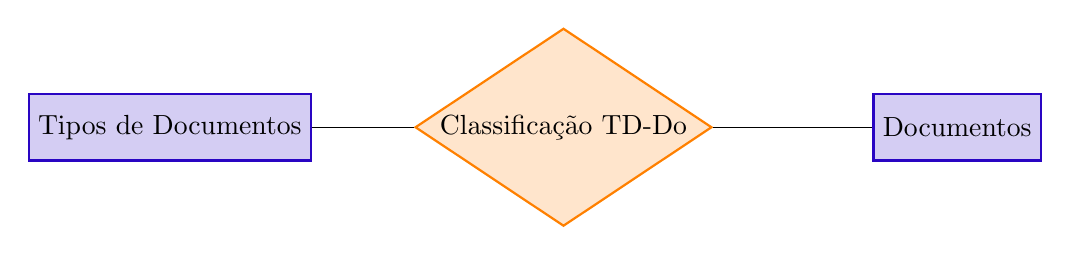
\begin{tikzpicture}
  [every entity/.style={fill=blue!20,draw=blue,thick},
   every relationship/.style={fill=orange!20,draw=orange,thick,aspect=1.5}]
  \node[entity] (TiposdeDocumentos)  at (0,0)   {Tipos de Documentos};
  \node[entity] (Documentos) at (10,0)   {Documentos};
  \node[relationship]    at (5,0) {Classifica\c{c}\~ao TD-Do}
    edge (TiposdeDocumentos)
    edge (Documentos);
\end{tikzpicture}

O Diagrama MER acima pode ser lido, da esquerda para direita como \textquotedbl Tipos de Documentos classificam Documentos\textquotedbl  e, no sentido inverso, \textquotedbl Documentos s\~ao classificados segundo Tipos de Documentos\textquotedbl .










\subsection[Associa\c{c}\~ao: Indexa\c{c}\~ao de Eventos (TA-Ev)]{Associa\c{c}\~ao: Indexa\c{c}\~ao de Eventos (TA-Ev)}\label{Associa\c{c}\~ao: Indexa\c{c}\~ao de Eventos (TA-Ev)}
J\'a foi comentado que os eventos do WASH (Ev) podem ser classificados pelo tipo de atividade (TA). Por exemplo: podemos ter um evento do tipo oficina, outro do tipo palestra, e assim por diante. Para essa indexa\c{c}\~ao ser\~ao utilizadas palavras-chave.










Esta situa\c{c}\~ao indica uma associa\c{c}\~ao entre a entidade \textquotedbl Eventos\textquotedbl  e \textquotedbl Tipos de Atividades\textquotedbl , como segue:











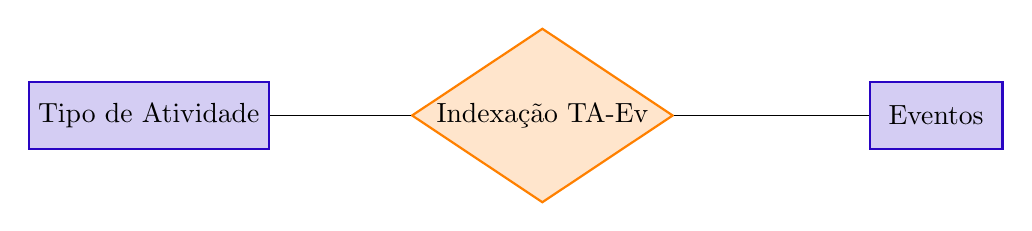
\begin{tikzpicture}
  [every entity/.style={fill=blue!20,draw=blue,thick},
   every relationship/.style={fill=orange!20,draw=orange,thick,aspect=1.5}]
  \node[entity] (TipodeAtividade)  at (0,0)   {Tipo de Atividade};
  \node[entity] (Eventos) at (10,0)   {Eventos};
  \node[relationship]    at (5,0) {Indexa\c{c}\~ao TA-Ev}
    edge (TipodeAtividade)
    edge (Eventos);
\end{tikzpicture}

A associa\c{c}\~ao acima pode ser lida, da esquerda para a direita, como: \textquotedbl Tipos de Atividades indexam Eventos\textquotedbl . Da direta para a esquerda, podemos ler como: \textquotedbl Eventos s\~ao indexados segundo Tipos de Atividades\textquotedbl .










N\~ao podemos desconsiderar a hip\'otese de que um mesmo evento pode estar associado a mais de uma atividade. Podemos ter um evento que, inicialmente, transcorreu na forma de Oficina e, depois, na forma de palestra. Podemos ter um evento que ocorre em duas salas diferentes. Na primeira podemos ter o formato de oficina e na segunda podemos ter o formato de Roda de Conversa. Por esse motivo, esta associa\c{c}\~ao deve prever essa possibilidade.










Esta pluralidade de atividades num mesmo evento nos motiva a n\~ao adotar o conceito de taxonomia para organizar os tipos de atividades, pelo menos por ora.










\subsection[Associa\c{c}\~ao: Indexa\c{c}\~ao de Eventos (Te-Ev)]{Associa\c{c}\~ao: Indexa\c{c}\~ao de Eventos (Te-Ev)}\label{Associa\c{c}\~ao: Indexa\c{c}\~ao de Eventos (Te-Ev)}
Os eventos do WASH tamb\'em podem ser indexados pelo tema abordado usando palavras chave, lembrando que um mesmo evento pode abordar mais de um tema.










A associa\c{c}\~ao pertinente pode ser representada como segue:











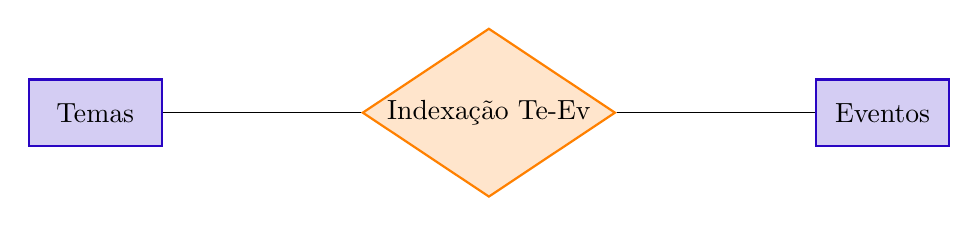
\begin{tikzpicture}
  [every entity/.style={fill=blue!20,draw=blue,thick},
   every relationship/.style={fill=orange!20,draw=orange,thick,aspect=1.5}]
  \node[entity] (Temas)  at (0,0)   {Temas};
  \node[entity] (Eventos) at (10,0)   {Eventos};
  \node[relationship]    at (5,0) {Indexa\c{c}\~ao Te-Ev}
    edge (Temas)
    edge (Eventos);
\end{tikzpicture}

A associa\c{c}\~ao indicada pode ser lida, da esquerda para direita, como segue: \textquotedbl Temas indexam Eventos\textquotedbl , ao passo que direita para  esquerda pode ser lida como \textquotedbl Eventos s\~ao indexados por Temas\textquotedbl .










Como vimos na defini\c{c}\~ao da entidade \textquotedbl Temas\textquotedbl  (Te), n\~ao adotaremos uma estrutura taxon\^omica para classific\'a-los, pelo menos por ora.










\subsection[Associa\c{c}\~ao: Classifica\c{c}\~ao das Institui\c{c}\~oes (TI-In)]{Associa\c{c}\~ao: Classifica\c{c}\~ao das Institui\c{c}\~oes (TI-In)}\label{Associa\c{c}\~ao: Classifica\c{c}\~ao das Institui\c{c}\~oes (TI-In)}
Assim como ocorre com rela\c{c}\~ao \`a entidade \textquotedbl Documentos\textquotedbl , tamb\'em existe uma taxonomia de \textquotedbl Institui\c{c}\~oes\textquotedbl . Isto significa que uma institui\c{c}\~ao pode ser associada a mais de um tipo de institui\c{c}\~ao, desde que estes tipos estejam dentro de um mesmo ramo da taxonomia. Esta situa\c{c}\~ao indica a exist\^encia de uma associa\c{c}\~ao como segue:











\begin{tikzpicture}
  [every entity/.style={fill=blue!20,draw=blue,thick},
   every relationship/.style={fill=orange!20,draw=orange,thick,aspect=1.5}]
  \node[entity] (TiposdeInstititui\c{c}\~oes)  at (0,0)   {Tipos de Instititui\c{c}\~oes};
  \node[entity] (Institui\c{c}\~oes) at (10,0)   {Institui\c{c}\~oes};
  \node[relationship]    at (5,0) {Classifica\c{c}\~ao TI-In}
    edge (TiposdeInstititui\c{c}\~oes)
    edge (Institui\c{c}\~oes);
\end{tikzpicture}

Da mesma forma como nos demais casos, da esquerda para a direita podemos ler \textquotedbl Tipos de Institui\c{c}\~oes classificam Institui\c{c}\~oes\textquotedbl  e, no sentido inverso, \textquotedbl Institui\c{c}\~oes s\~ao classificadas pelo Tipo de Institui\c{c}\~oes\textquotedbl .










\subsection[Associa\c{c}\~ao: Desempenho de Papel (In-PI-Ev)]{Associa\c{c}\~ao: Desempenho de Papel (In-PI-Ev)}\label{Associa\c{c}\~ao: Desempenho de Papel (In-PI-Ev)}
De forma semelhante ao que acontece na associa\c{c}\~ao \textquotedbl Desempenho P-TP-I\textquotedbl , que indica o desempenho de \textquotedbl Tipos de Papeis\textquotedbl  por \textquotedbl Pessoas\textquotedbl  vinculadas a \textquotedbl Institui\c{c}\~oes\textquotedbl , podemos ter os \textquotedbl Papeis das Institui\c{c}\~oes\textquotedbl  desempenhados por \textquotedbl Institui\c{c}\~oes\textquotedbl  no \^ambito de \textquotedbl Eventos\textquotedbl .










Vimos que a Portaria CTI 178/2018 prev\^e alguns papeis especiais para as institui\c{c}\~oes, no \^ambito do WASH, tais como:











\begin{alineas}
\item Institui\c{c}\~oes Promotoras
\item Institui\c{c}\~oes Executoras
\item Institui\c{c}\~oes Respons\'aveis
\end{alineas}

Vimos que uma institui\c{c}\~ao pode assumir um ou mais papeis durante um evento, e diferentes papeis para eventos diferentes.










(Nota: o termo \textquotedbl entidade\textquotedbl  \'e usado no sentido de \textquotedbl institui\c{c}\~ao\textquotedbl  na Portaria 178/2018. Para evitar confus\~ao com o conceito de \textquotedbl entidades\textquotedbl  do Modelo MER, aqui ser\'a substitu\'{\i}do por \textquotedbl institui\c{c}\~ao\textquotedbl .)










Por exemplo: o CTI j\'a foi, simultaneamente, \textquotedbl Institui\c{c}\~ao Promotora\textquotedbl  e \textquotedbl Institui\c{c}\~ao Respons\'avel\textquotedbl  em alguns eventos, ao passo que em outros o CTI atuou apenas como \textquotedbl Institui\c{c}\~ao Promotora\textquotedbl . O IFSP j\'a foi apenas \textquotedbl Institui\c{c}\~ao Respons\'avel\textquotedbl  para alguns eventos, sendo \textquotedbl Institui\c{c}\~ao Promotora\textquotedbl  para outros. Essa variedade de papeis requer uma associa\c{c}\~ao do tipo tern\'aria, como segue:











\begin{tikzpicture}
  [every entity/.style={fill=blue!20,draw=blue,thick},
   every relationship/.style={fill=orange!20,draw=orange,thick,aspect=1.5}]
  \node[entity] (Institui\c{c}\~ao)  at (0,0)   {Institui\c{c}\~ao};
  \node[entity] (PapeisdasInstitui\c{c}\~oes) at (10,0)   {Papeis das Institui\c{c}\~oes};
  \node[entity] (Eventos) at (5,-3)   {Eventos};
  \node[relationship]    at (5,0) {Desempenho In-PI-Ev}
    edge (Institui\c{c}\~ao)
    edge (PapeisdasInstitui\c{c}\~oes)
    edge (Eventos)
	;
\end{tikzpicture}

Denominados a asssocia\c{c}\~ao como \textquotedbl Desempenho In-PI-Ev\textquotedbl , com \textquotedbl In\textquotedbl  para Institui\c{c}\~oes, \textquotedbl PI\textquotedbl  para \textquotedbl Papeis das Institui\c{c}\~oes\textquotedbl  e \textquotedbl Ev\textquotedbl  para \textquotedbl Eventos\textquotedbl .










Esta associa\c{c}\~ao pode ser lida, da esquerda para direita como segue: \textquotedbl As Institui\c{c}\~oes desempenham Papeis nos Eventos\textquotedbl . Da direita para a esquerda, a associa\c{c}\~ao pode ser lida como segue: \textquotedbl Papeis s\~ao desempenhados por Institui\c{c}\~oes nos Eventos\textquotedbl .










\subsection[Associa\c{c}\~ao: Organiza\c{c}\~ao de Tipos de Processos (In-Tr)]{Associa\c{c}\~ao: Organiza\c{c}\~ao de Tipos de Processos (In-Tr)}\label{Associa\c{c}\~ao: Organiza\c{c}\~ao de Tipos de Processos (In-Tr)}
A associa\c{c}\~ao \textquotedbl In-Tr\textquotedbl  relaciona a entidade \textquotedbl Tipos de Processos\textquotedbl  (Tr) com as Institui\c{c}\~oes (In). Propusemos essa associa\c{c}\~ao considerando que cada institui\c{c}\~ao tem seus tipos de processos, que, um a um, definem as caracter\'{\i}sticas dos documentos que s\~ao vinculados a um elemento da entidade \textquotedbl Processos\textquotedbl . O uso verbo \textquotedbl ter\textquotedbl  (veja acima \textquotedbl institui\c{c}\~ao tem\textquotedbl ), indica uma associa\c{c}\~ao de pertencimento, raz\~ao do nome da associa\c{c}\~ao.










Por exemplo: o CNPq tem dois tipos processos principais, pertinentes ao WASH:











\begin{alineas}
\item Processos-M\~ae, que s\~ao relacionados a uma emenda parlamentar e agrupam os processos das bolsas
\item Processos das bolsas, propriamente ditos, que s\~ao agrupados em Processos-M\~ae
\end{alineas}

O Governo Federal tem, por exemplo, processos administrativos referentes \`as nomea\c{c}\~oes de servidores a cargos comissionados, que definem os ocupantes de cargos de diretor em unidades dos Institutos Federais ou em Unidades de Pesquisa do Minist\'erio de Ci\^encia, Tecnologia e Inova\c{c}\~oes.











\begin{tikzpicture}
  [every entity/.style={fill=blue!20,draw=blue,thick},
   every relationship/.style={fill=orange!20,draw=orange,thick,aspect=1.5}]
  \node[entity] (Insititui\c{c}\~oes)  at (0,0)   {Insititui\c{c}\~oes};
  \node[entity] (TiposdeProcessos) at (10,0)   {Tipos de Processos};
  \node[relationship]    at (5,0) {Organiza\c{c}\~ao In-Tr}
    edge (Insititui\c{c}\~oes)
    edge (TiposdeProcessos);
\end{tikzpicture}

A associa\c{c}\~ao acima, em linguagem natural, pode ser lida, da esquerda para direita, como: Institui\c{c}\~oes possuem tipos de processos administrativos.










Da direita para a esquerda a associa\c{c}\~ao acima pode ser lida como: Os \textquotedbl Tipos de Processos\textquotedbl  s\~ao caracter\'{\i}sticos das \textquotedbl Institui\c{c}\~oes\textquotedbl .










\subsection[Associa\c{c}\~ao: Classifica\c{c}\~ao de Processos (Tr-Pr)]{Associa\c{c}\~ao: Classifica\c{c}\~ao de Processos (Tr-Pr)}\label{Associa\c{c}\~ao: Classifica\c{c}\~ao de Processos (Tr-Pr)}
Os processos da entidade \textquotedbl Processos\textquotedbl  precisam ser organizados em \textquotedbl Tipos de Processos\textquotedbl , raz\~ao pela qual existe a associa\c{c}\~ao \textquotedbl Tipifica\c{c}\~ao Tr-Pr\textquotedbl , como segue:











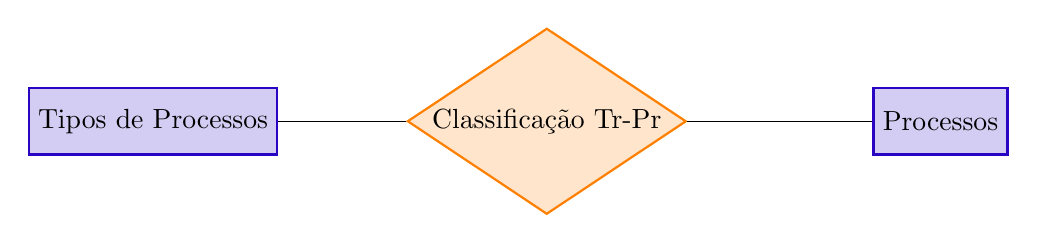
\begin{tikzpicture}
  [every entity/.style={fill=blue!20,draw=blue,thick},
   every relationship/.style={fill=orange!20,draw=orange,thick,aspect=1.5}]
  \node[entity] (TiposdeProcessos)  at (0,0)   {Tipos de Processos};
  \node[entity] (Processos) at (10,0)   {Processos};
  \node[relationship]    at (5,0) {Classifica\c{c}\~ao Tr-Pr}
    edge (TiposdeProcessos)
    edge (Processos);
\end{tikzpicture}

A associa\c{c}\~ao indicada acima pode ser lida, da esquerda para a direita, como segue: \textquotedbl Tipos de Processos\textquotedbl  classificam os \textquotedbl Processos\textquotedbl . Da direita para a esquerda, podemos ler: os \textquotedbl Processos\textquotedbl  s\~ao classificados segundo \textquotedbl Tipos de Processos\textquotedbl .










Note que esta associa\c{c}\~ao \textquotedbl trabalha\textquotedbl  em conjunto com a associa\c{c}\~ao \textquotedbl In-Tr\textquotedbl  para associar um dado processo com uma dada institui\c{c}\~ao.










\subsection[Associa\c{c}\~ao: Organiza\c{c}\~ao de Documentos (Pr-Do)]{Associa\c{c}\~ao: Organiza\c{c}\~ao de Documentos (Pr-Do)}\label{Associa\c{c}\~ao: Organiza\c{c}\~ao de Documentos (Pr-Do)}
Como j\'a dito, o WASH \'e realizado no \^ambito p\'ublico, em que os documentos s\~ao organizados em Processos Administrativos.










Desta forma, propomos que seja estabelecida uma associa\c{c}\~ao entre os documentos e processos administrativos, permitindo agrupar os documentos:











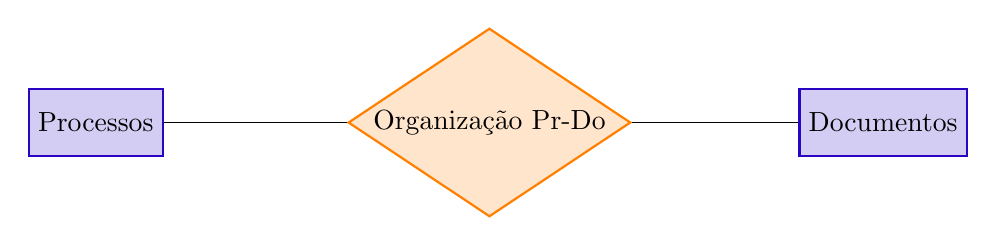
\begin{tikzpicture}
  [every entity/.style={fill=blue!20,draw=blue,thick},
   every relationship/.style={fill=orange!20,draw=orange,thick,aspect=1.5}]
  \node[entity] (Processos)  at (0,0)   {Processos};
  \node[entity] (Documentos) at (10,0)   {Documentos};
  \node[relationship]    at (5,0) {Organiza\c{c}\~ao Pr-Do}
    edge (Processos)
    edge (Documentos);
\end{tikzpicture}

A associa\c{c}\~ao acima pode ser lida, em linguagem natural, da esquerda para a direita, como: \textquotedbl Processos\textquotedbl  organizam \textquotedbl Documentos\textquotedbl .










Da direita para a esquerda a associa\c{c}\~ao pode ser lida como: \textquotedbl Documentos\textquotedbl  podem ser organizados em \textquotedbl Processos\textquotedbl .










\'E importante notar que existem dois caminhos para relacionar documentos com institui\c{c}\~oes:











\begin{alineas}
\item associa\c{c}\~ao \textquotedbl Desempenho Pe-TP-In-Do\textquotedbl , que relaciona uma pessoa (Pe) com um tipo de papel (TP) que \'e desempenhado no \^ambito de um v\'{\i}nculo com uma institui\c{c}\~ao (In), conforme documentado 
(Do).
\item o encadeamento das associa\c{c}\~oes \textquotedbl Organiza\c{c}\~ao In-Tr\textquotedbl , \textquotedbl Classifica\c{c}\~ao Tr-Pr\textquotedbl  e \textquotedbl Organiza\c{c}\~ao Pr-Do\textquotedbl , que indica a qual processo (Pr) o Documento (Do) est\'a vinculado, permitindo relacionar o processo (Pr) com o tipo de processo (Tr) que, por sua vez, est\'a vinculado a uma institui\c{c}\~ao (In).
\end{alineas}

Note que estes dois \textquotedbl caminhos\textquotedbl  representam informa\c{c}\~oes diferentes. O caminho (a) indica o documento (Do) que al\c{c}a a pessoa (Pe) a um certo papel (TP) dentro do WASH no contexto de um v\'{\i}nculo com uma determinada institui\c{c}ao (In), mas este documento n\~ao \'e necessariamente emitido pela institui\c{c}\~ao \`a qual aquele v\'{\i}nculo se refere.










Por exemplo: o coordenador do WASH (Pe), servidor p\'ublico de uma unidade de pesquisa (In, e.g. Cemaden), pode emitir declara\c{c}\~ao (Do) de que um determinado bolsista (Pe) tem bolsa do CNPq (TP), num determinado processo (Pr). O documento foi emitido por servidor da unidade de pesquisa (Pe) para declarar que o bolsista (Pe) est\'a vinculado ao WASH por meio de bolsa do CNPq (TP). Isso significa que um documento (Do) emitido por representante da institui\c{c}\~ao A (In) pode ser usado para comprovar o v\'{\i}nculo de um participante com a institui\c{c}\~ao B (In). Portanto, esse caminho \'e usado, principalmente, para registrar a que institui\c{c}\~ao (In) uma pessoa (Pe) est\'a vinculada.










O caminho (b) permite relacionar um documento (Do) a uma pessoa (Pe) no contexto de um processo (Pr). Esse caminho \'e utilizado para guardar planos de trabalho, relat\'orios, publica\c{c}\~oes, etc.










Finalmente, no que se refere a esta associa\c{c}\~ao de \textquotedbl Organiza\c{c}\~ao\textquotedbl , cabe ressaltar que um documento (Do) pode estar associado apenas a um processo (Pr). Em outras palavras, dois processos (Pr) diferentes n\~ao podem conter um mesmo documento.










\subsection[Associa\c{c}\~ao: Organiza\c{c}\~ao de Localiza\c{c}\~ao (In-Ci)]{Associa\c{c}\~ao: Organiza\c{c}\~ao de Localiza\c{c}\~ao (In-Ci)}\label{Associa\c{c}\~ao: Organiza\c{c}\~ao de Localiza\c{c}\~ao (In-Ci)}
\'E preciso saber a localiza\c{c}\~ao das atividades e isso \'e feito atrav\'es de uma associa\c{c}\~ao entre Institui\c{c}\~oes (In) e Cidades (Ci), como segue:











\begin{tikzpicture}
  [every entity/.style={fill=blue!20,draw=blue,thick},
   every relationship/.style={fill=orange!20,draw=orange,thick,aspect=1.5}]
  \node[entity] (Institui\c{c}\~oes)  at (0,0)   {Institui\c{c}\~oes};
  \node[entity] (Cidades) at (10,0)   {Cidades};
  \node[relationship]    at (5,0) {Organiza\c{c}\~ao In-Ci}
    edge (Institui\c{c}\~oes)
    edge (Cidades);
\end{tikzpicture}

Esta associa\c{c}\~ao pode ser lida, da esquerda para a direita, como: \textquotedbl Institui\c{c}\~oes est\~ao localizadas em cidades\textquotedbl . Da direita para a esquerda pode ser lida como: \textquotedbl Cidades abrigam institui\c{c}\~oes\textquotedbl . A substantiva\c{c}\~ao mais adequada para esses dois verbos \'e \textquotedbl localiza\c{c}\~ao\textquotedbl , mas utilizaremos a palavra \textquotedbl organiza\c{c}\~ao\textquotedbl  para seguir a nomenclatura at\'e aqui utilizada, enfatizando que n\~ao se trata de taxonomia nem de indexa\c{c}\~ao.










\subsection[Modelagem BPMN]{Modelagem BPMN}\label{Modelagem BPMN}
Por indica\c{c}\~ao do coordenador do Projeto WASH, foi desenvolvida uma modelagem BPMN nos processos do WASH. O trabalho foi conduzido por Saulo Monteiro, que baseado nos fluxos de processo desenvolvidos pela equipe do WASH, produziu o modelo apresentado na fig. XXX.












\captionsetup{format=plain}
\begin{figure}[htb]

	\begin{center}

		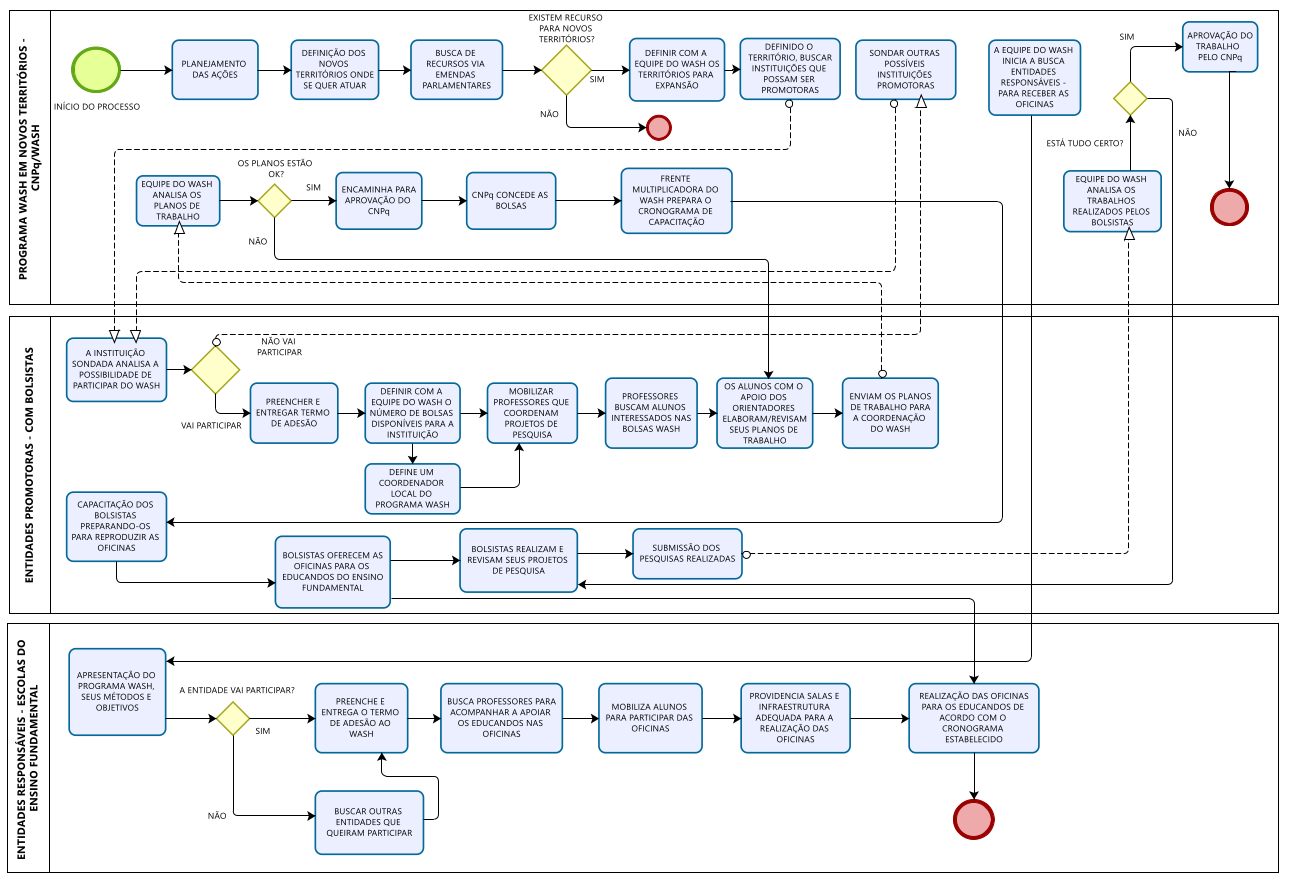
\includegraphics[max size={\textwidth}{\textheight}]{../../imagens/bizagi.png}

	\end{center}

	\caption{\label{17b9e2dc78c8926a87c5d8e8c0c9568cb175db59}Modelagem BPMN dos processos do WASH (cr\'editos: Saulo Monteiro).}

\end{figure}

\subsection[S\'{\i}ntese: o funcionamento do Programa WASH]{S\'{\i}ntese: o funcionamento do Programa WASH}\label{S\'{\i}ntese: o funcionamento do Programa WASH}
Com base em toda a modelagem conduzida at\'e aqui, \'e poss\'{\i}vel validar o entendimento existente sobre o funcionamento do Programa WASH. Para isso, nos baseamos num dos relat\'orios apresentados ao CNPq, referente \`a emenda parlamentar executada no Estado do Paran\'a, entre 2020 e 2021  (WASHCNPq, 2022).










A escolha desse relat\'orio em particular, dentre v\'arios apresentados ao CNPq ao longo destes 10 anos, se deve ao fato de ser um dos mais recentes, o qual reflete a maturidade do entendimento do que de fato \'e o WASH. A presente candidata \'e co-autora do referido documento. As informa\c{c}\~oes sobre o funcionamento do WASH presentes no relat\'orio foram balizadas e confrontadas com o que a modelagem nos trouxe, bem como com os dados presentes na Platu\'oxe. Outros documentos do acervo tamb\'em foram usados como refer\^encia, sendo citados oportunamente ao longo do texto.










Iniciamos nossa an\'alise identificando um dos elementos mais importantes presentes em WASHCNPq (2022): o conceito de multiplica\c{c}\~ao. Segundo a refer\^encia:











\noindent\begin{center}\mbox{\centering\fbox{\centering\par\parbox{0.7\linewidth}{\small\textit{\textquotedbl (...) Um dos aspectos fundamentais do projeto \'e a forma\c{c}\~ao de multiplicadores, porque a multiplica\c{c}\~ao ocorre a partir de estudantes do ensino m\'edio, t\'ecnico e superior, que, com a forma\c{c}\~ao e acompanhamento oferecidos pela equipe da Frente Multiplicadora, promovem oficinas e exercem o papel de monitores para educandos do ensino fundamental, sempre com conhecimento e consentimento do respons\'avel legal.\textquotedbl  (Fonte:  WASHCNPq (2022))}\normalsize}}}\end{center}


Esta afirma\c{c}\~ao pode ser constatada atrav\'es da inspe\c{c}\~ao dos dados de eventos registrados na plataforma Platu\'oxe, onde se verifica a realiza\c{c}\~ao de forma\c{c}\~oes de multiplicadores, por meio de reuni\~oes da Frente Multiplicadora. Esses jovens, depois, aparecem em oficinas no \^ambito das escolas de ensino fundamental. Em termos de modelagem, observa-se a possibilidade de um participante (representado na entidade \textquotedbl Pessoas\textquotedbl ) assumir v\'arios papeis, tais como o de bolsista, multiplicador, educando, etc.










\'E poss\'{\i}vel identificar no WASH uma preocupa\c{c}\~ao com o respeito ao papel que cada participante pode desempenhar, em fun\c{c}\~ao da peculiaridade de cada um. Com rela\c{c}\~ao a isso WASHCNPq (2022) revela que o entendimento de que o multiplicador n\~ao deve assumir para si a fun\c{c}\~ao de um docente, em rela\c{c}\~ao \`as crian\c{c}as benefici\'arias. Esse papel \'e exclusivo dos profissionais habilitados e reconhecidos para tal. Assim,  as oficinas devem transcorrer na presen\c{c}a de adultos capacitados e legalmente respons\'aveis pelas crian\c{c}as.










Sobre a restri\c{c}\~ao exposta acima, vemos que o anexo \`a Portaria CTI 178/2018 antecipa a necessidade de uma entidade respons\'avel na opera\c{c}\~ao do WASH, normalmente a escola onde as crian\c{c}as est\~ao matriculadas. Esse entidade deve designar o profissional habilitado que deve estar presente no momento da oficina, juntamente com o multiplicador.










O multiplicador, em geral, \'e tamb\'em um bolsista de inicia\c{c}\~ao cient\'{\i}fica. Vem sendo reconhecido no \^ambito da academia, embora n\~ao seja normatizada, a previs\~ao aproximada de dedica\c{c}\~ao de um bolsista de inicia\c{c}\~ao cient\'{\i}fica ao seu projeto.










\section[Caracteriza\c{c}\~ao dos Indicadores do WASH (eixo 3)]{Caracteriza\c{c}\~ao dos Indicadores do WASH (eixo 3)}\label{Caracteriza\c{c}\~ao dos Indicadores do WASH (eixo 3)}
Como visto na se\c{c}\~ao da Fundamenta\c{c}\~ao Te\'orica e em Materiais e M\'etodos, o objetivo da coleta de dados \'e produzir indicadores que, analisados e interpretados, tragam informa\c{c}\~oes sobre o projeto, complementando as demais dimens\~oes deste estudo de forma quantitativa, contribuindo para a caracteriza\c{c}\~ao do Programa WASH.










S\~ao exemplos de indicadores a serem apresentados nesta se\c{c}\~ao:











\begin{alineas}
\item n\'umero de pessoas atendidas
\item evolu\c{c}\~ao temporal do n\'umero de pessoas atendidas
\item n\'umero de bolsistas
\item n\'umero de relat\'orios
\item distribui\c{c}\~ao de temas abordados em relat\'orios
\item n\'umero de oficinas realizadas
\item distribui\c{c}\~ao et\'aria dos participantes em oficina
\item distribui\c{c}\~ao de temas nas oficinas
\item distribui\c{c}\~ao das atividades nas oficinas
\item quantidade de cidades atendidas
\item participantes mais ass\'{\i}duos
\item muitos outros.
\end{alineas}

Importante registrar que os dados a seguir foram obtidos a partir da contribui\c{c}\~ao de v\'arios colaboradores do WASH, com nossa participa\c{c}\~ao ativa na especifica\c{c}\~ao dos sistemas de coleta de dados, a exemplo da Plataforma Platu\'osh, da qual a presente candidata \'e co-autora  (MAMMANA et al., 2022).










Tr\^es fontes principais de dados foram utilizadas para gerar os indicadores:











\begin{alineas}
\item Plataforma Platu\'osh: voltada inicialmente para o registro da quantidade de eventos realizados e n\'umero de participantes em cada evento, bem como dos testemunhos documentais e fotogr\'aficos dessa realiza\c{c}\~ao e participa\c{c}\~ao. Posteriormente a Platu\'osh foi sendo adaptada para incluir dados gerenciais (vincula\c{c}\~oes e afilia\c{c}\~oes institucionais), bem como registro de acervo (documentos gerados ao longo do projeto). Como esta plataforma est\'a em plena opera\c{c}\~ao, com dados sendo adicionados diariamente, foi preciso escolher um recorte temporal para a presente an\'alise. Desta forma, os dados aqui presentes referem-se ao per\'{\i}odo de setembro de 2013 a 26 de agosto de 2022.
\item Plataforma de Planejamento Financeiro do Programa WASH: plataforma de acompanhamento das concess\~oes de bolsas, suas validades, documentos de outorgas, planos de trabalho. Trata-se de uma ferramenta de compliance e presta\c{c}\~ao de contas do projeto, mas que tamb\'em pode ser usada para a caracteriza\c{c}\~ao do mesmo, pela abrang\^encia dos dados nela contida.
\item Planilhas digitais de dados constru\'{\i}das pela candidata manualmente (sem uso do sistema de entrada de dados automatizado): instrumento criado separadamente pela candidata para viabilizar a verifica\c{c}\~ao dos dados das demais plataformas, uma vez que foram identificadas algumas fragilidades nas demais fontes de informa\c{c}\~oes.
\end{alineas}

\subsection[Amostragem do p\'ublico atendido]{Amostragem do p\'ublico atendido}\label{Amostragem do p\'ublico atendido}
Antes de prosseguir \'e preciso explicitar que uma parte dos indicadores utilizados neste projeto, principalmente aqueles referentes \`a Platu\'osh, foram obtidos por amostragem, uma vez que o Programa WASH tem limita\c{c}\~oes na coleta de dados cadastrais de participantes.










Estas limita\c{c}\~oes foram discutidas no cap\'{\i}tulo de Materiais e M\'etodos e est\~ao relacionadas \`a falta de atribui\c{c}\~ao legal para que o projeto colete dados cadastrais de seus participantes, tornando facultativo o compartilhamento destas informa\c{c}\~oes pelas entidades parceiras (executoras, promotoras e respons\'aveis).










Portanto, tem ocorrido recorrentemente a falta de registro, nos arquivos do WASH, dos participantes que est\~ao sob cust\'odia da Entidade Respons\'avel. Esta situa\c{c}\~ao se intensificou a partir da edi\c{c}\~ao da Lei Geral de Prote\c{c}\~ao de Dados. Tudo indica que as responsabilidades impostas aos gestores escolares por essa lei t\^em aumentado a  resist\^encia, por parte dos parceiros, em compartilhar informa\c{c}\~oes de participa\c{c}\~ao dos estudantes, o que \'e perfeitamente compreens\'{\i}vel.










Assim, no que tange \`a caracteriza\c{c}\~ao do p\'ublico participante, \'e preciso usar o m\'etodo de amostragem.










Antecipadamente, para evitar que o leitor tenha uma vis\~ao inicial equivocada sobre a representatividade estat\'{\i}stica dos dados aqui apresentados, \'e preciso fazer uma ressalva, \`a qual retornaremos in\'umeras vezes neste texto.










Ocorre que a redu\c{c}\~ao recente do fornecimento de dados por parte dos parceiros resultou em uma mudan\c{c}a no perfil de amostragem, dificultando a compara\c{c}\~ao dos indicadores anuais do projeto. Esta quest\~ao ser\'a tratada mais adiante.










Reconhecer a ocorr\^encia dessa mudan\c{c}a de perfil da coleta de dados ao longo dos anos de exist\^encia do projeto \'e importante para que se tenha a real no\c{c}\~ao da validade dos valores globais e das m\'edias apresentadas deste ponto em diante.










No que se refere \`a distribui\c{c}\~ao de participantes por sexo, foi aplicado um m\'etodo de amostragem especial, principalmente para os casos em que o cadastro era incompleto e n\~ao havia informa\c{c}\~ao individualizada sobre sexo. O Cap\'{\i}tulo de Materias e M\'etodos detalha como esta identifica\c{c}\~ao \`a posteriore do sexo dos participantes foi feita mas, sumariamente, podemos dizer que ela se deu por meio da identifica\c{c}\~ao do g\^enero do primeiro nome de cada particip1ante, por meio da compara\c{c}\~ao desse primeiro nome com listas de nomes extensivas, dividos por g\^enero.










Em termos de recorte temporal, os dados aqui apresentados referem-se ao per\'{\i}odo de 2013 (quando o WASH foi criado) at\'e o dia 26 de agosto de 2022, quando foi feita uma c\'opia da base de dados visando a an\'alise.










Para conhecer o n\'umero de cadastros na base de dados \'e preciso fazer uma consulta sobre a tabela \textquotedbl participantes2\textquotedbl , por meio da linguagem SQL.










O uso da linguagem SQL escapa ao escopo de conhecimento desta candidata. No entanto, como as consultas foram baseadas em nossas solicita\c{c}\~oes \`a equipe de TI, pudemos propor que tais consultas fossem \textquotedbl traduzidas\textquotedbl  para o portugu\^es.










Para saber o n\'umero de cadastrados na tabela participantes2, que traz todos os cadastrados na plataforma Platu\'osh, utilizamos o equivalente \`a seguinte consulta:











\noindent\begin{center}\mbox{\centering\fbox{\centering\par\parbox{0.7\linewidth}{\small\textit{selecione a contagem de nome\_de\_participantes da tabela participantes2;}\normalsize}}}\end{center}













Esta consulta, segundo os colaboradores de TI, \'e feita por meio do comando SQL a seguir:











\noindent\begin{center}\mbox{\centering\fbox{\centering\par\parbox{0.7\linewidth}{\small\textit{select count(nome\_participante) from participantes2;}\normalsize}}}\end{center}













O resultado obtido com esta consulta, para os dados congelados em 26 de agosto de 2022, foi de 3.312 (tr\^es mil,trezentos e doze) participantes.










Mas, por inspe\c{c}\~ao da lista de participantes, ainda segundo os colaboradores da TI, \'e poss\'{\i}vel identificar que h\'a cadastros repetidos, resultantes, provavelmente, de erros de digita\c{c}\~ao.










Felizmente, a linguagem SQL permite excluir os cadastros repetidos, tarefa que foi delegada \`a prestimosa equipe de TI do WASH. Para isso, foi constru\'{\i}da uma nova consulta, que pode ser traduzida para o portugu\^es como segue:











\noindent\begin{center}\mbox{\centering\fbox{\centering\par\parbox{0.7\linewidth}{\small\textit{selecione a contagem de nomes\_de\_participantes distintos, da tabela participantes2;}\normalsize}}}\end{center}













Esta consulta, no SQL original \'e feita pelo comando a seguir:











\noindent\begin{center}\mbox{\centering\fbox{\centering\par\parbox{0.7\linewidth}{\small\textit{select count(distinct nome\_participante) from participantes2;}\normalsize}}}\end{center}













Assim, pelo emprego da consulta acima, foi poss\'{\i}vel identificar um n\'umero de participantes com nomes distintos, com um total de 3265 (tr\^es mil duzentos e sessenta e cinco) pessoas.










O conjunto de 47 pessoas, que \'e a diferen\c{c}a entre o n\'umero com nomes incluindo as repeti\c{c}\~oes (3312 participantes) e o n\'umero sem nomes repetidos (3265 participantes) pode conter duas situa\c{c}\~oes:











\begin{alineas}
\item cadastros repetidos referentes \`a mesma pessoa
\item hom\^onimos
\end{alineas}

Mas os bancos relacionais nos permitem conhecer um pouco melhor o motivo pelo qual aparecem nomes repetidos. Para isso, \'e poss\'{\i}vel utilizar o ano de nascimento, que tamb\'em \'e registrado no cadastro.










A probabilidade de dois participantes terem exatamente o mesmo nome e terem nascido no mesmo ano \'e substancialmente menor do que a simples ocorr\^encia de hom\^onimos. Assim, foi solicitado \`a TI que fossem considerados como cadastros repetidos aqueles que t\^em nomes repetidos e anos repetidos. A consulta \`a base de dados, em portugu\^es, ficou assim:











\noindent\begin{center}\mbox{\centering\fbox{\centering\par\parbox{0.7\linewidth}{\small\textit{selecione a contagem de participantes agrupados por nome\_do\_participante e ano\_do\_nascimento;}\normalsize}}}\end{center}


Este comando, na linguagem SQL, novamente segundo os colaboradores da TI, pode ser expresso como segue:











\noindent\begin{center}\mbox{\centering\fbox{\centering\par\parbox{0.7\linewidth}{\small\textit{select count(*) as conta from participantes2 group by nome\_participante, ano\_nascimento;}\normalsize}}}\end{center}


O resultado desta consulta indica a exist\^encia de 3306 (tr\^es mil e trezentos e seis) participantes com nome e ano de nascimento simultaneamente diferentes. No entanto, uma an\'alise mais cuidadosa, conduzida pela equipe de TI a pedido desta candidata, indica que n\~ao h\'a a ocorr\^encia de hom\^onimos entre os 3312 (tr\^es mil, trezentos e doze) registros existentes na tabela  participantes2 pelos motivos que ser\~ao expressos a seguir.










A afirma\c{c}\~ao de que os 47 cadastros com nomes repetidos n\~ao se referem a hom\^onimos se sustenta nas seguintes evid\^encias:











\begin{alineas}
\item as repeti\c{c}\~oes de nomes identificadas na base s\~ao bastante incomuns, incluindo formas estrangeiras de nomes pr\'oprios combinadas, o que afasta a hip\'otese de hom\^onimos. Este fato, por si s\'o seria um indicativo de que provavelmente estas repeti\c{c}\~oes se referem \`a mesma pessoa, havendo um indevido cadastramento duplicado para 47 pessoas.
\item Quando o nome repetido \'e confrontado com o ano de nascimento, percebe-se que os dois registros com mesmo nome se diferem pela aus\^encia do dado do ano de nascimento para um dos registros com nome repetido, ou mesmo para os dois, situa\c{c}\~ao que inviabiliza o crit\'erio de agrupamento de nome e ano de nascimento, como forma de identificar hom\^onimos.
\end{alineas}

Desta forma, \'e poss\'{\i}vel afirmar que o n\'umero de registros v\'alidos no WASH \'e de 3265 (tr\^es mil duzentos e sessenta e cinco) participantes e h\'a um erro de cerca de 1,4\% nos registros totais (47 repeti\c{c}\~oes em 94 registros). Este n\'umero de erros \'e relativamente pequeno para o universo de participantes.










Um outro aspecto que precisa ser bastante enfatizado \'e que o n\'umero efetivo de participantes no WASH \'e provavelmente substancialmente maior do que 3265 (tr\^es mil, duzentos e sessenta e cinco) registrados, superando o que est\'a efetivamente registrado na plataforma.










Para sustentar esta afirma\c{c}\~ao, \'e poss\'{\i}vel considerar que muitas oficinas do projeto foram realizadas em recintos sem controle de entrada, impedindo que um cadastro individualizado fosse feito.










Mas esta afirma\c{c}\~ao n\~ao teria validade se n\~ao fosse poss\'{\i}vel apresentar evid\^encias de eventos com essas caracter\'{\i}sticas, mostrando que o n\'umero de participantes, nos casos exemplificados, foi maior do que o de efetivamente cadastrados.










Desta forma, passamos a apresentar exemplos de eventos em que tal situa\c{c}\~ao ocorreu, adicionando evid\^encias fotogr\'aficas de que o n\'umero de registrados na plataforma n\~ao reflete o alcance real do projeto. Por uma raz\~ao de espa\c{c}o, limitamos essa exposi\c{c}\~ao a 7 casos, como segue:











\begin{alineas}
\item evento de grande porte realizado no CTI Renato Archer, ocorrido em 11 de abril de 2015, quando centenas de crian\c{c}as participaram do Ci\^encia em Show, trupe de artistas formados em f\'{\i}sica. Os registros oficiais indicam a presen\c{c}a de 5 pessoas, o que n\~ao se coaduna com os registro fotogr\'aficos, que indicam um p\'ublico de 20 a 40 vezes maior.
\item comemora\c{c}\~ao do dia das crian\c{c}as realizada em 3 de outubro de 2015, com atividades musicais e culturais. Os registros da plataforma, neste dia, apontam para a participa\c{c}\~ao de 9 participantes, mas os registros fotogr\'aficos do evento apontam para uma presen\c{c}a muito superior.
\item Evento de confraterniza\c{c}\~ao de Natal realizado no CTI Renato Archer, com palestras e outras atividades l\'udicas, realizado em 19 de dezembro de 2015, com registro de 8 participantes, mas os registros fotogr\'aficos indicam a participa\c{c}\~ao de substancialmente maior de crian\c{c}as.
\item Evento Greenk, patrocinado pelo MCTI, que aconteceu no Expo Center Anhembi em S\~ao Paulo, na semana de 27 de maio de 2018. O porte do evento e n\'umero de dias de realiza\c{c}\~ao indicam uma quantidade substancialmente maior do que registrado: 13 pessoas. Essa discrep\^ancia se deu porque o tipo de evento n\~ao permitia o cadastro de p\'ublico, ficando os registros restritos aos bolsistas multiplicadores, bem com aos demais respons\'aveis.
\item Em 23 de junho de 2018 o Programa WASH promoveu uma visita ao Museu Aberto de Astronomia- MAAS, em Campinas. Os registros oficiais n\~ao trazem o n\'umero de participantes, mas os registros fotogr\'aficos indicam a presen\c{c}a de v\'arias dezenas de crian\c{c}as.
\item evento em pra\c{c}a p\'ublica realizado na cidade de Prado Ferreira (PR), em 31 de maio de 2019. No evento em quest\~ao foi poss\'{\i}vel estimar uma presen\c{c}a de v\'arias centenas de pessoas, com a pra\c{c}a tomada pelo p\'ublico. O evento envolveu o lan\c{c}amento do Programa WASH na cidade, no \^ambito do Programa Profiss\~ao 4.0, criado em lei municipal, cuja elabora\c{c}\~ao da Lei teve orienta\c{c}\~ao e colabora\c{c}\~ao ativa desta candidata [XXX].
\item Evento Dia da Fam\'{\i}lia na Escola, realizado na EMEF Milton Pereira Costa, em Guarulhos, no dia 27 de novembro de 2021, com a presen\c{c}a de um dos membros do Ci\^encia em Show. O p\'ublico estimado est\'a em cerca de 2 centenas, mas n\~ao houve registro individualizado pelo aspecto amplo do evento.
\end{alineas}



\captionsetup{format=plain}
\begin{figure}[max size={\textwidth}{\textheight}]

\centering


\begin{minipage}[b]{0.4\linewidth}
        \centering
                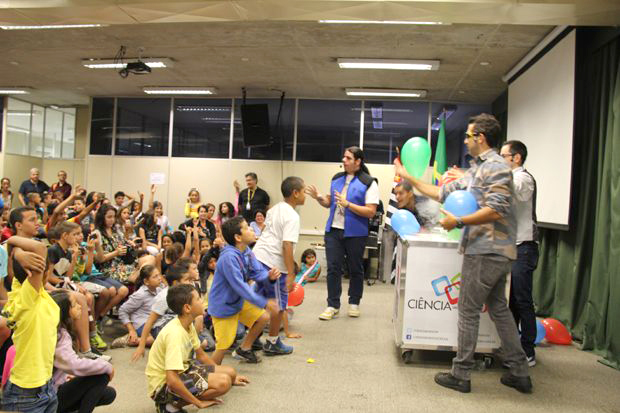
\includegraphics[width=1.0\linewidth]{../../imagens/Evento-Ciencia-Em-Show.jpg}
                \caption{Evento de demonstra\c{c}\~oes cient\'{i}ficas realizado no \^ambito do WASH em 11 de abril de 2015, com a participa\c{c}\~ao do Ci\^encia em Show, trupe de artistas formados em f\'{i}sica que promoviam a ci\^encia na televis\~ao. O car\'ater amplo do evento n\~ao permitiu controlar a presen\c{c}a de participantes que pode ser estimada em perto de duas centenas de crian\c{c}as.}
                \label{5340059e38852932c32c5ce8624858fef8a1f3f0}
\end{minipage}%
\hspace{0.5cm}
\begin{minipage}[b]{0.4\linewidth}
        \centering
                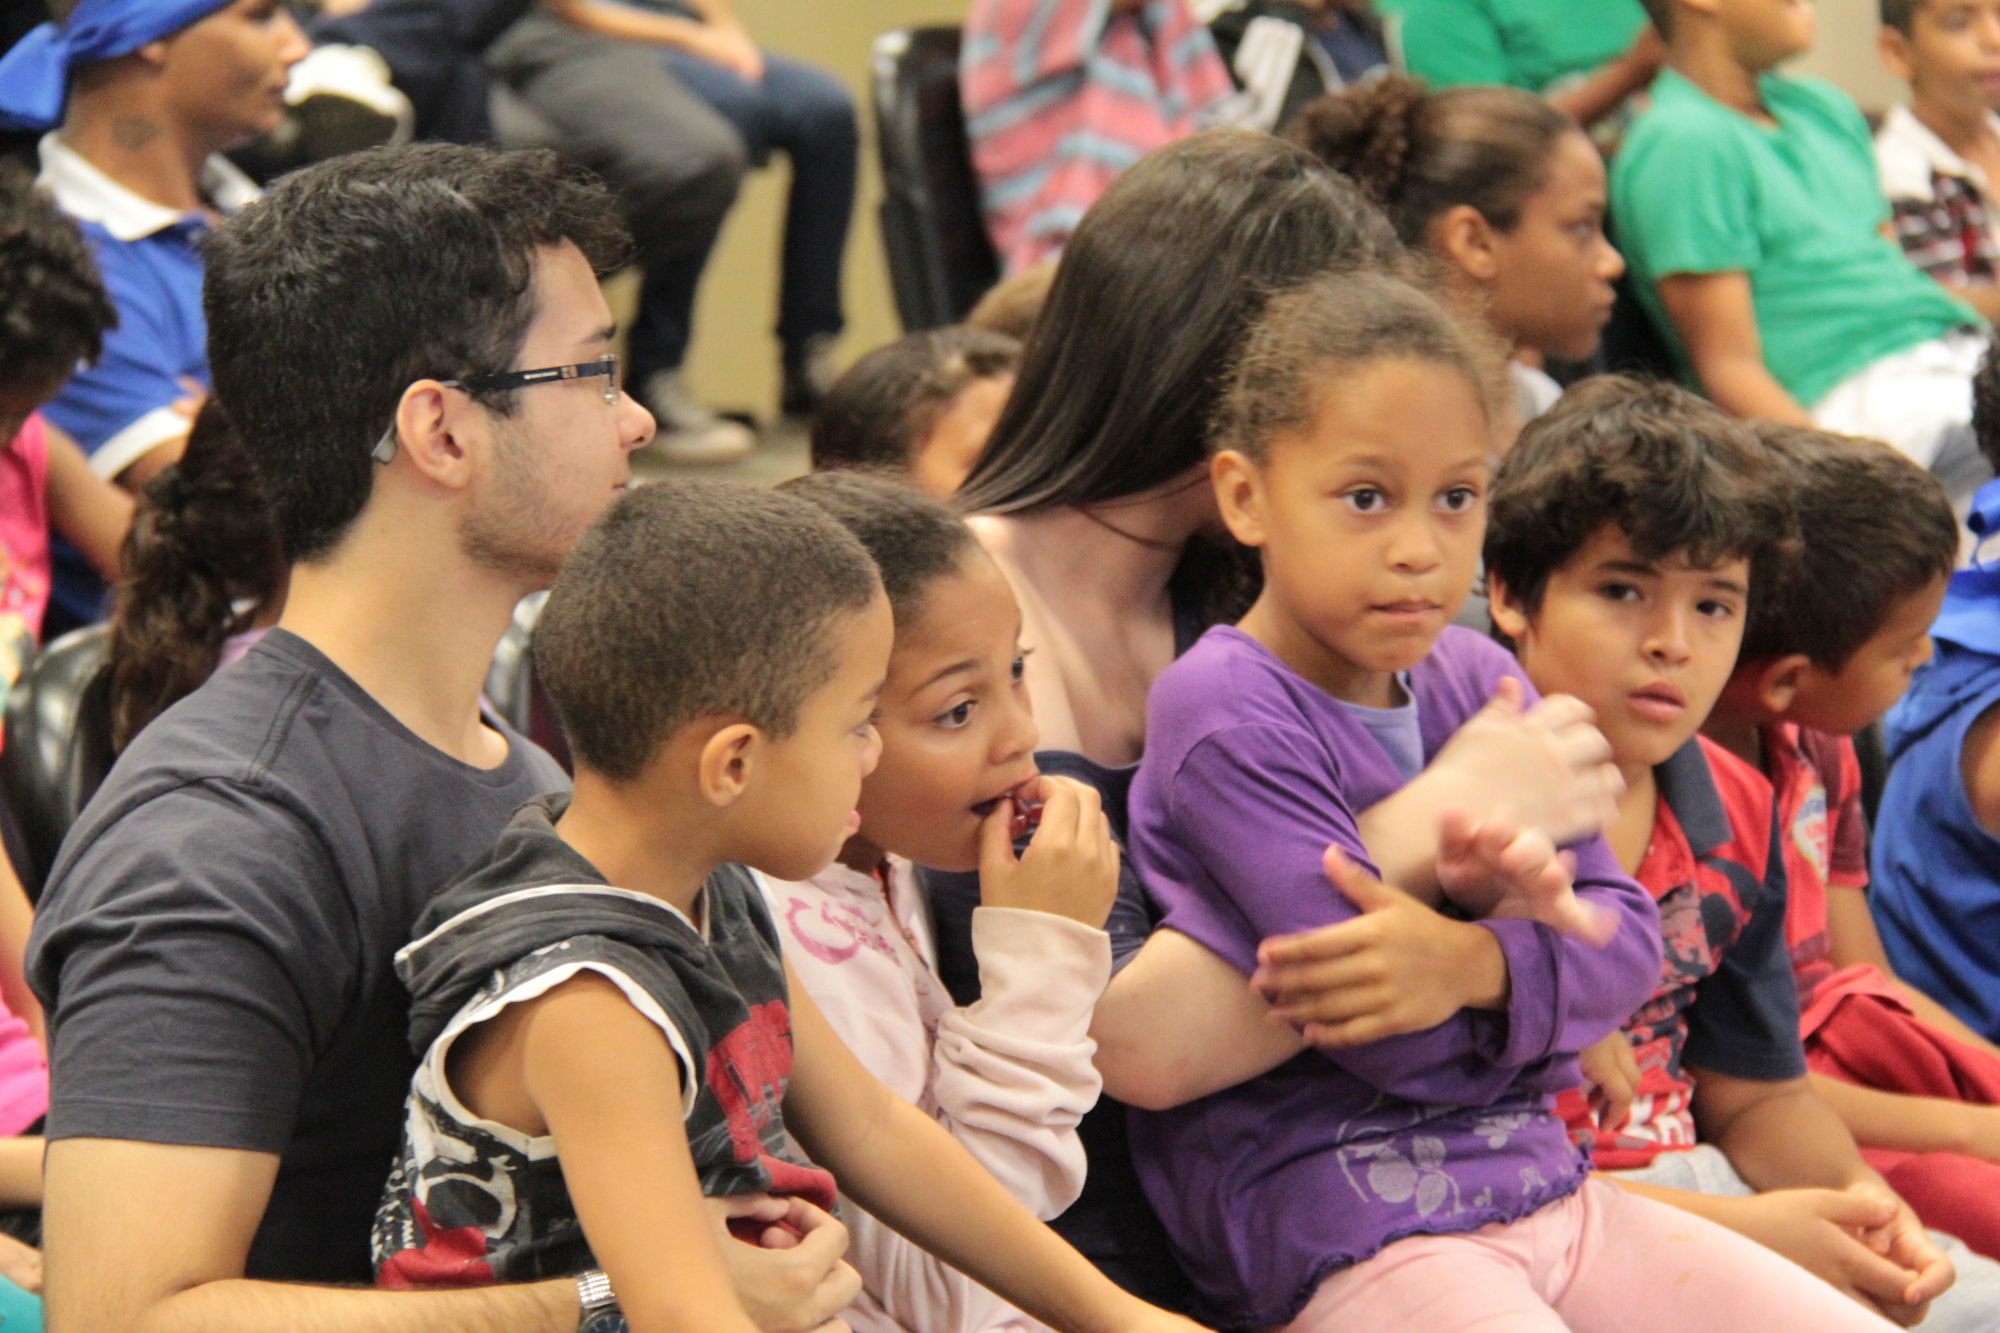
\includegraphics[width=1.0\linewidth]{../../imagens/dia-das-criancas-2022-10-03-menor.JPG}
                \caption{Evento de comemora\c{c}\~ao do dia das crian\c{c}as, com atividades musicais e culturais. Os registros da plataforma apontam para 9 participantes, mas os registros fotogr\'aficos indicam uma presen\c{c}a muito maior.}
                \label{31e991b69f3aba382518bb571a4e69a720fa8ccb}
\end{minipage}
\hspace{0.5cm}
\begin{minipage}[b]{0.4\linewidth}
        \centering
                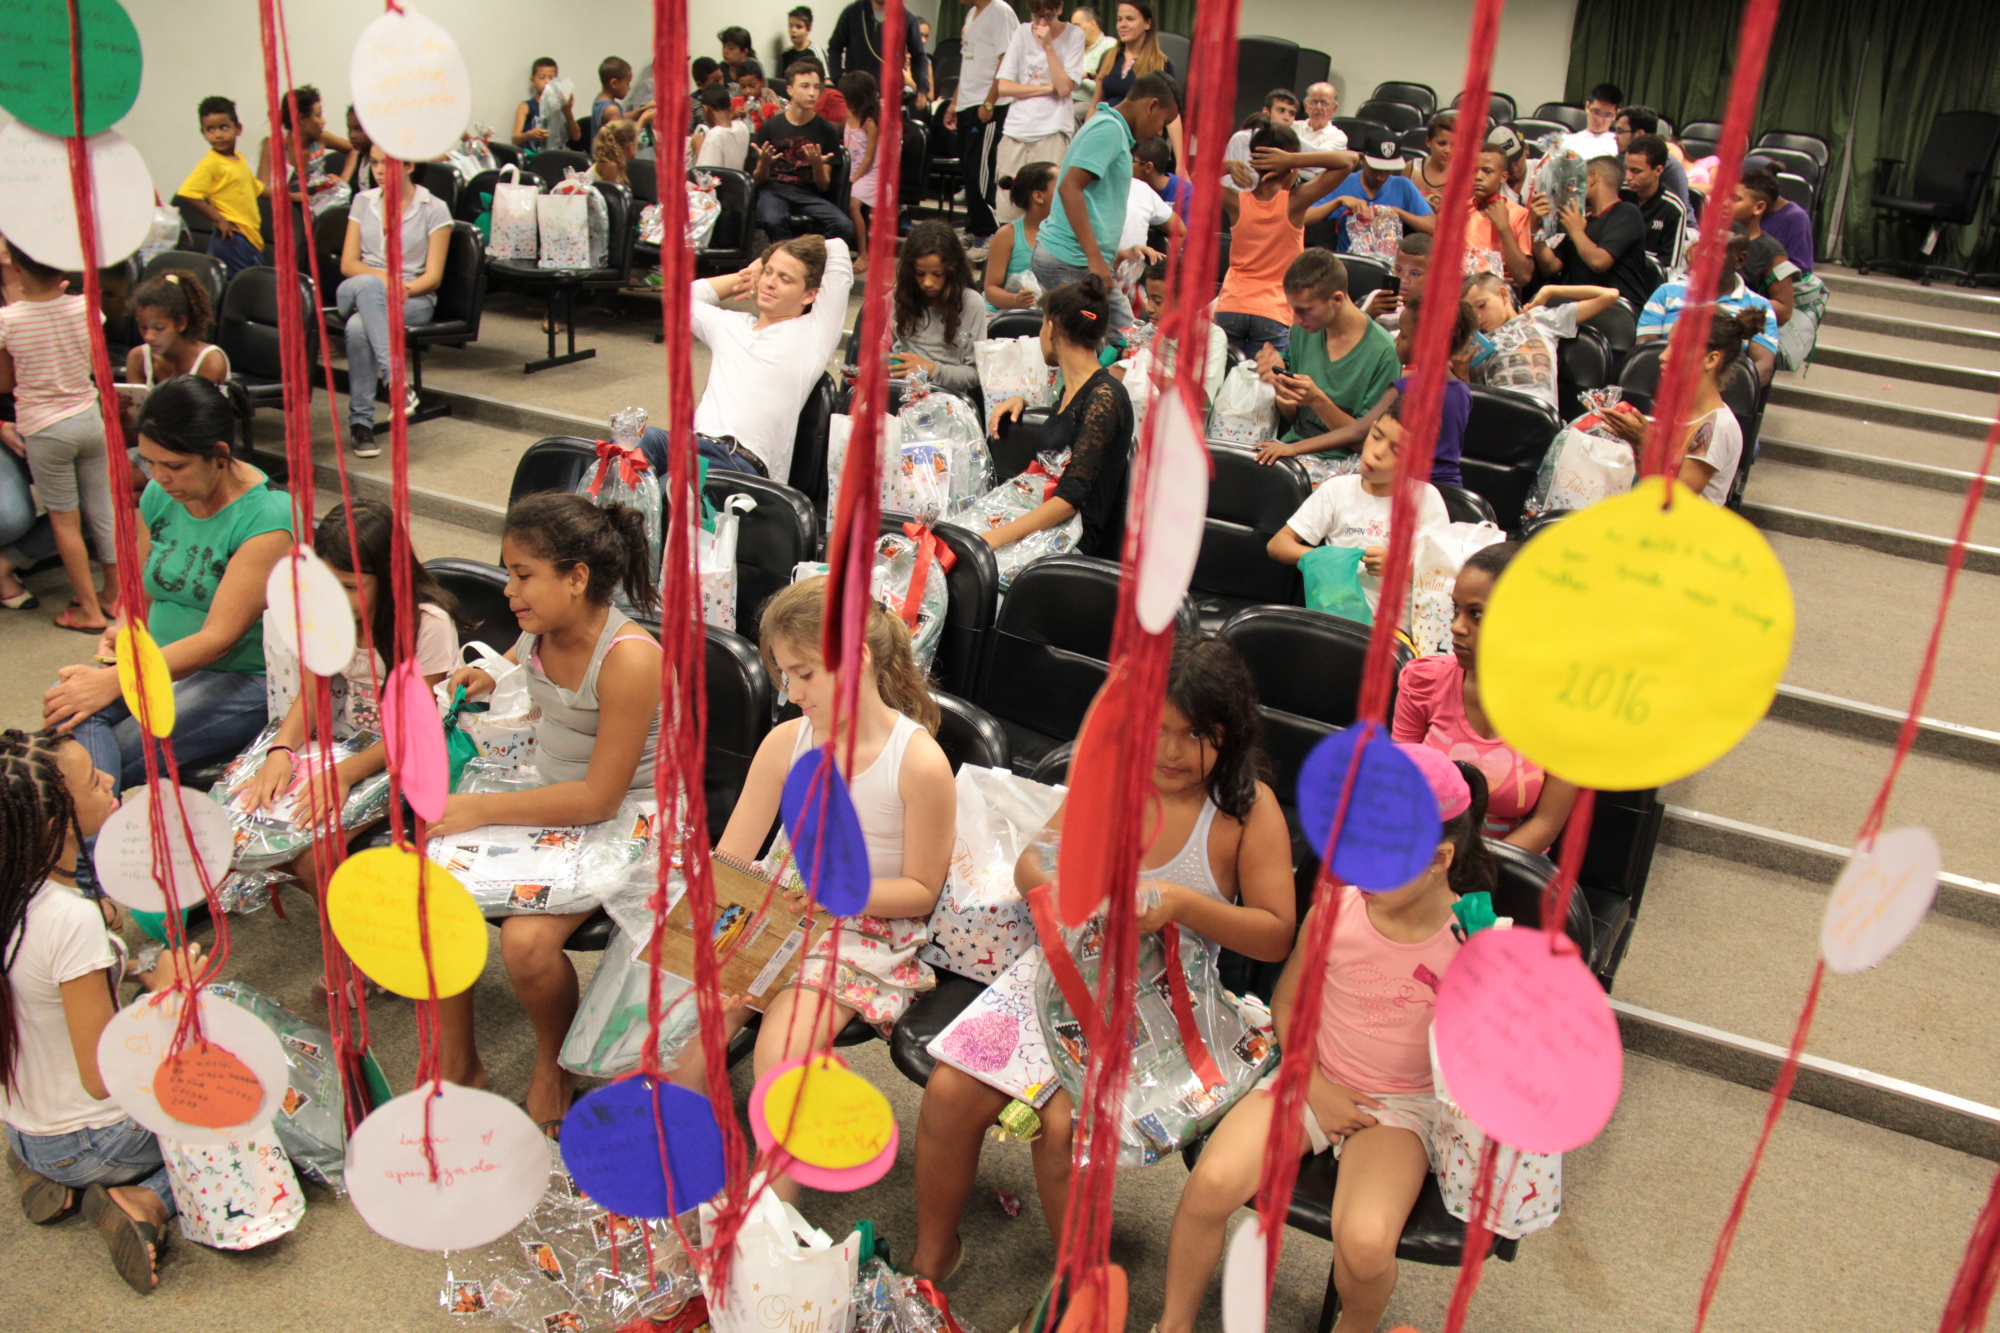
\includegraphics[width=1.0\linewidth]{../../imagens/confraternizacao-de-natal-menor.jpeg}
                \caption{Evento de Natal realizado no CTI Renato Archer em 19 de dezembro de 2015. O evento incluiu uma variada gama de atividades l\'udicas e educacionais. Muito embora o registro oficial indique a participa\c{c}\~ao de 8 pessoas, as fotos mostram que a quantidade foi muito superior.}
                \label{afa1b2acd7f4c590f25d9821e48e82568bd28cf2}
\end{minipage}%
\hspace{0.5cm}
\begin{minipage}[b]{0.4\linewidth}
        \centering
                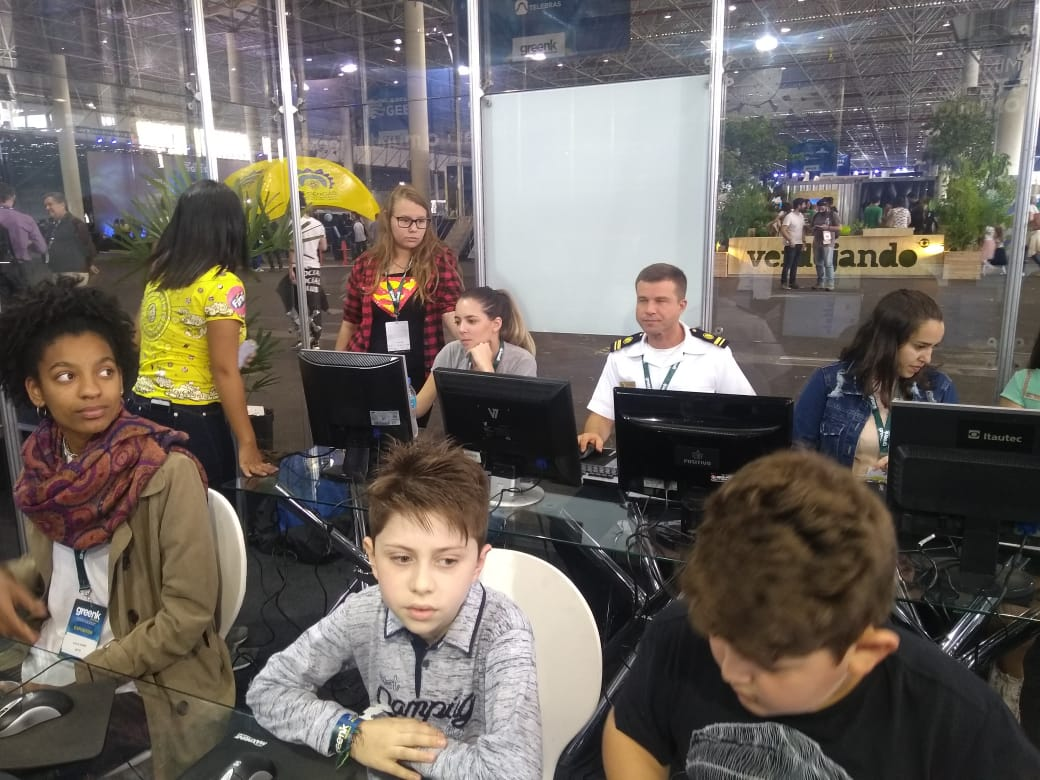
\includegraphics[width=1.0\linewidth]{../../imagens/Evento-Greenk-2018-05-27.jpg}
                \caption{Evento Greenk, patrocinado pelo MCTI no Expo Center Anhembi em 27 de maio de 2018, que contou com oficinas do WASH. Neste tipo de evento \'e dif\'{i}cil realizar o cadastro nominal de participantes pela amplitude do mesmo. O p\'ublico beneficiado pode ser estimado em algumas centenas de crian\c{c}as.}
                \label{04766cbd557212dbb84969d429be542b364bf87a}
\end{minipage}
\hspace{0.5cm}
\begin{minipage}[b]{0.4\linewidth}
        \centering
                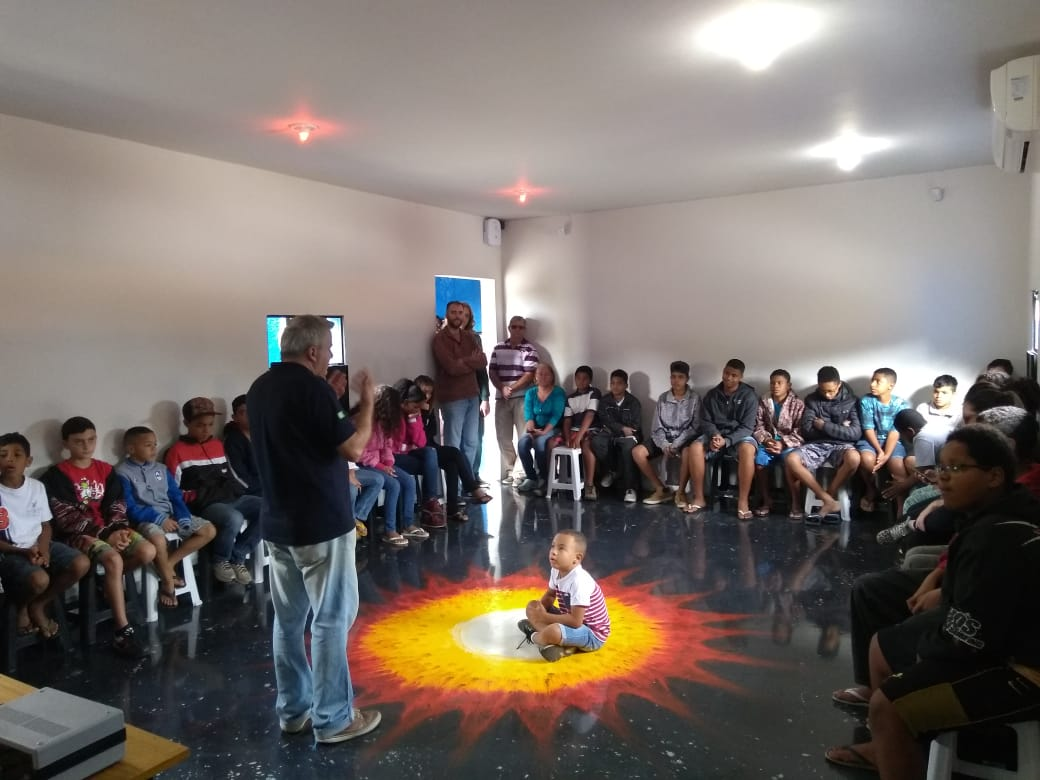
\includegraphics[width=1.0\linewidth]{../../imagens/MAAS.jpg}
                \caption{Evento no Museu Aberto de Astronomia, promovido pelo WASH. Os registros oficiais n\~ao indicam o n\'umero de participantes, mas os registros fotogr\'aficos mostram a participa\c{c}\~ao de dezenas de crian\c{c}as.}
                \label{b5542509570e0bcdbabe4949f7fef484141b805e}
\end{minipage}%
\hspace{0.5cm}
\begin{minipage}[b]{0.4\linewidth}
        \centering
                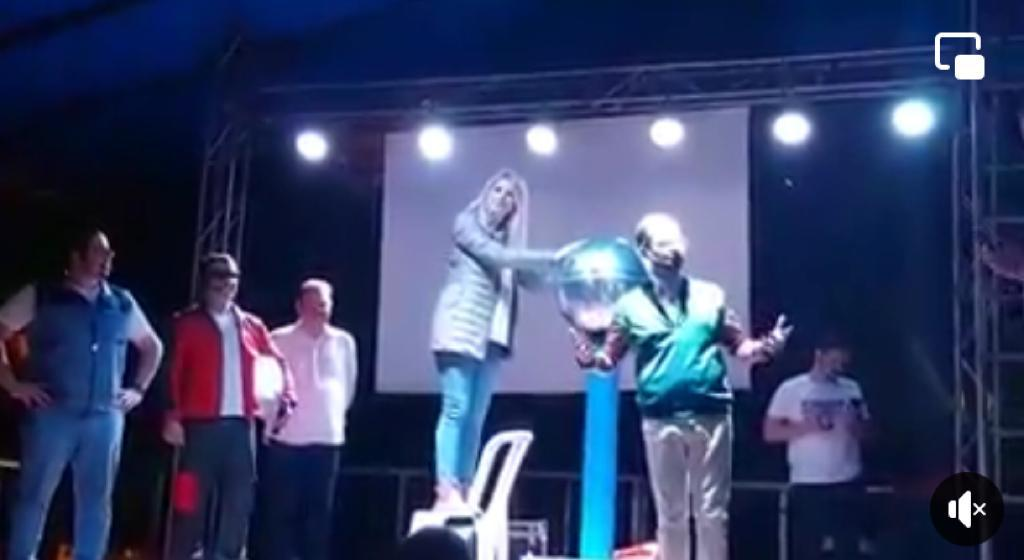
\includegraphics[width=1.0\linewidth]{../../imagens/Ciencia-em-Show-prado.jpeg}
                \caption{Evento de demonstra\c{c}\~oes cient\'{i}ficas na pra\c{c}a de Prado Ferreira, ocorrido em 31 de maio de 2019, cidade onde o WASH realizou dezenas de oficinas naquele per\'{i}odo. O evento foi promovido pelo WASH no lan\c{c}amento do Programa Profiss\~ao 4.0 na cidade e contou com a participa\c{c}\~ao do Ci\^encia em Show, trupe de artistas formados em f\'{i}sica com grande presen\c{c}a na m\'{i}dia televisiva.}
                \label{d76eb1e41d3d1e1394e18aafa3beb2bc3ad09471}
\end{minipage}
\hspace{0.5cm}
\end{figure}
















\captionsetup{format=plain}
\begin{figure}[max size={\textwidth}{\textheight}]

\centering


\begin{minipage}[b]{0.4\linewidth}
        \centering
                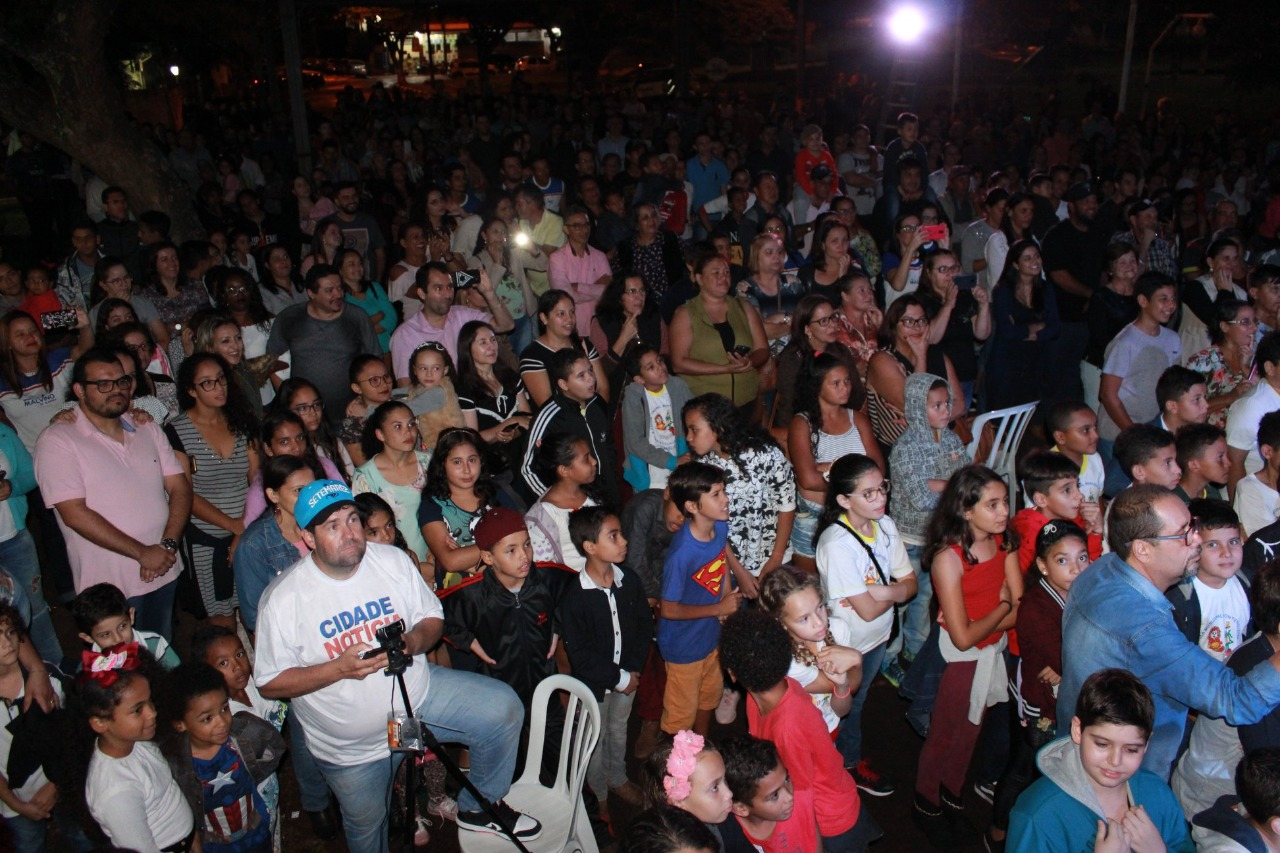
\includegraphics[width=1.0\linewidth]{../../imagens/Ciencia-Prado-publico.jpeg}
                \caption{P\'ublico no evento do Ci\^encia em Show}
                \label{7b56c85cc265fcbf261a3bc788ae1e4619b70725}
\end{minipage}%
\hspace{0.5cm}
\end{figure}



Com os registros at\'e aqui apresentados, n\~ao exaustivos, uma vez que foram selecionados apenas 7 exemplos num universo de milhares de eventos, buscamos sustentar a afirma\c{c}\~ao de que os 3265 cadastros de participantes representa uma amostra modesta de todos os benefici\'arios do Programa WASH.










N\~ao obstante esse car\'ater amostral, ou seja, incompleto em termos de registros individuais dos participantes, sustentamos que esses dados amostrais s\~ao imprescind\'{\i}veis para extrair importantes informa\c{c}\~oes sobre o projeto. Entre elas est\'a o seu crescimento org\^anico e o impacto da pandemia, por exemplo, o que pode ser verificado no gr\'afico a seguir.










\subsection[Evolu\c{c}\~ao temporal do n\'umero de participa\c{c}\~oes]{Evolu\c{c}\~ao temporal do n\'umero de participa\c{c}\~oes}\label{Evolu\c{c}\~ao temporal do n\'umero de participa\c{c}\~oes}
Na se\c{c}\~ao anterior foi mostrado que os dados de participantes presentes na Platu\'osh s\~ao uma amostra do total de participantes, uma vez que h\'a eventos em que n\~ao foi poss\'{\i}vel cadastrar todos participantes, a exemplo dos eventos que ocorrem em ambientes abertos (pra\c{c}as p\'ublicas, exposi\c{c}\~oes, etc.).










Foi comentado, tamb\'em, que em muitos casos os parceiros preferem n\~ao compartilhar dados cadastrais e de participa\c{c}\~ao de estudantes por raz\~oes de seguran\c{c}a de dados, tendo sido observado um crescimento nessa tend\^encia ao longo dos anos do projeto, principalmente a partir da edi\c{c}\~ao da Lei Geral de Prote\c{c}\~ao de Dados. Tal evolu\c{c}\~ao tem mudado o perfil de coleta de dados amostrais por parte do WASH.










Mesmo com essas dificuldades, os dados amostrais s\~ao importante para identificar tend\^encias do projeto, a exemplo da evolu\c{c}\~ao anual no n\'umero de participa\c{c}\~oes, mostrada abaixo:












\captionsetup{format=plain}
\begin{figure}[max size={\textwidth}{\textheight}]

\centering


\begin{minipage}[b]{0.4\linewidth}
        \centering
                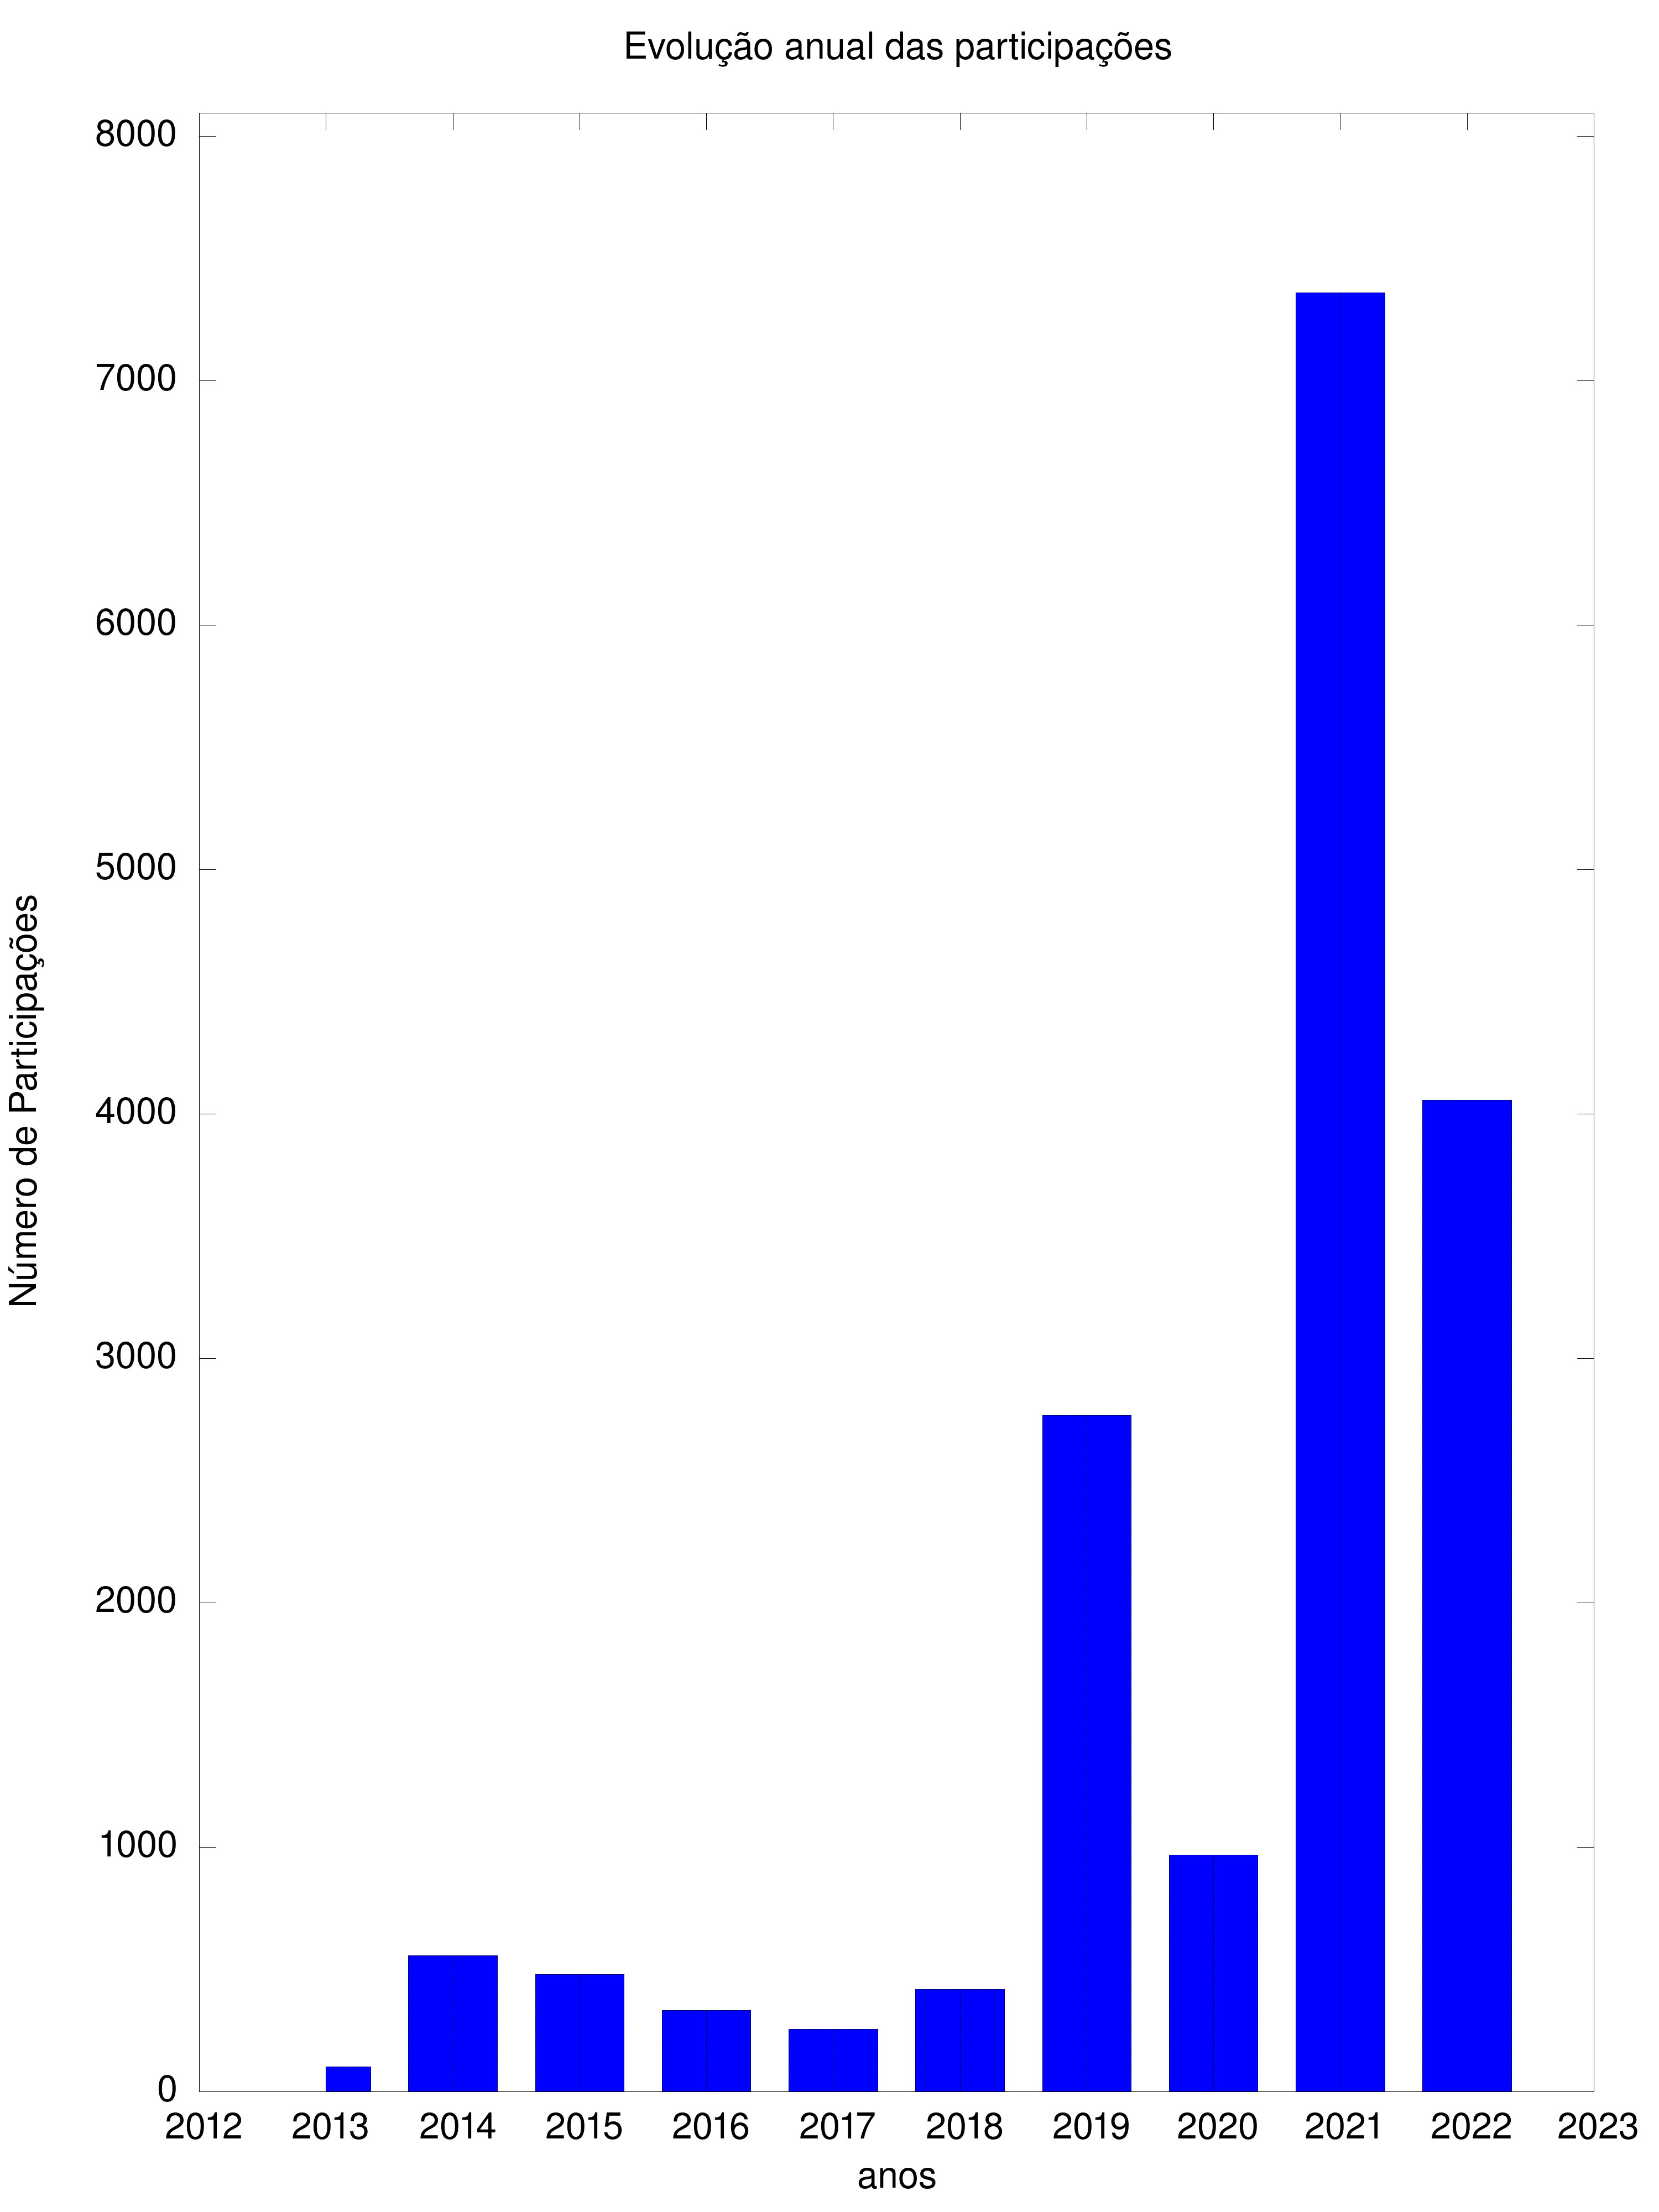
\includegraphics[width=1.0\linewidth]{../../imagens/output-participantes.jpeg}
                \caption{Evolu\c{c}\~ao temporal do n\'umero de participa\c{c}\~oes ao longo dos 10 anos de exist\^encia do Programa WASH.}
                \label{19699bcc5ab8317274249d6743d62534dbfb95fa}
\end{minipage}%
\hspace{0.5cm}
\begin{minipage}[b]{0.4\linewidth}
        \centering
                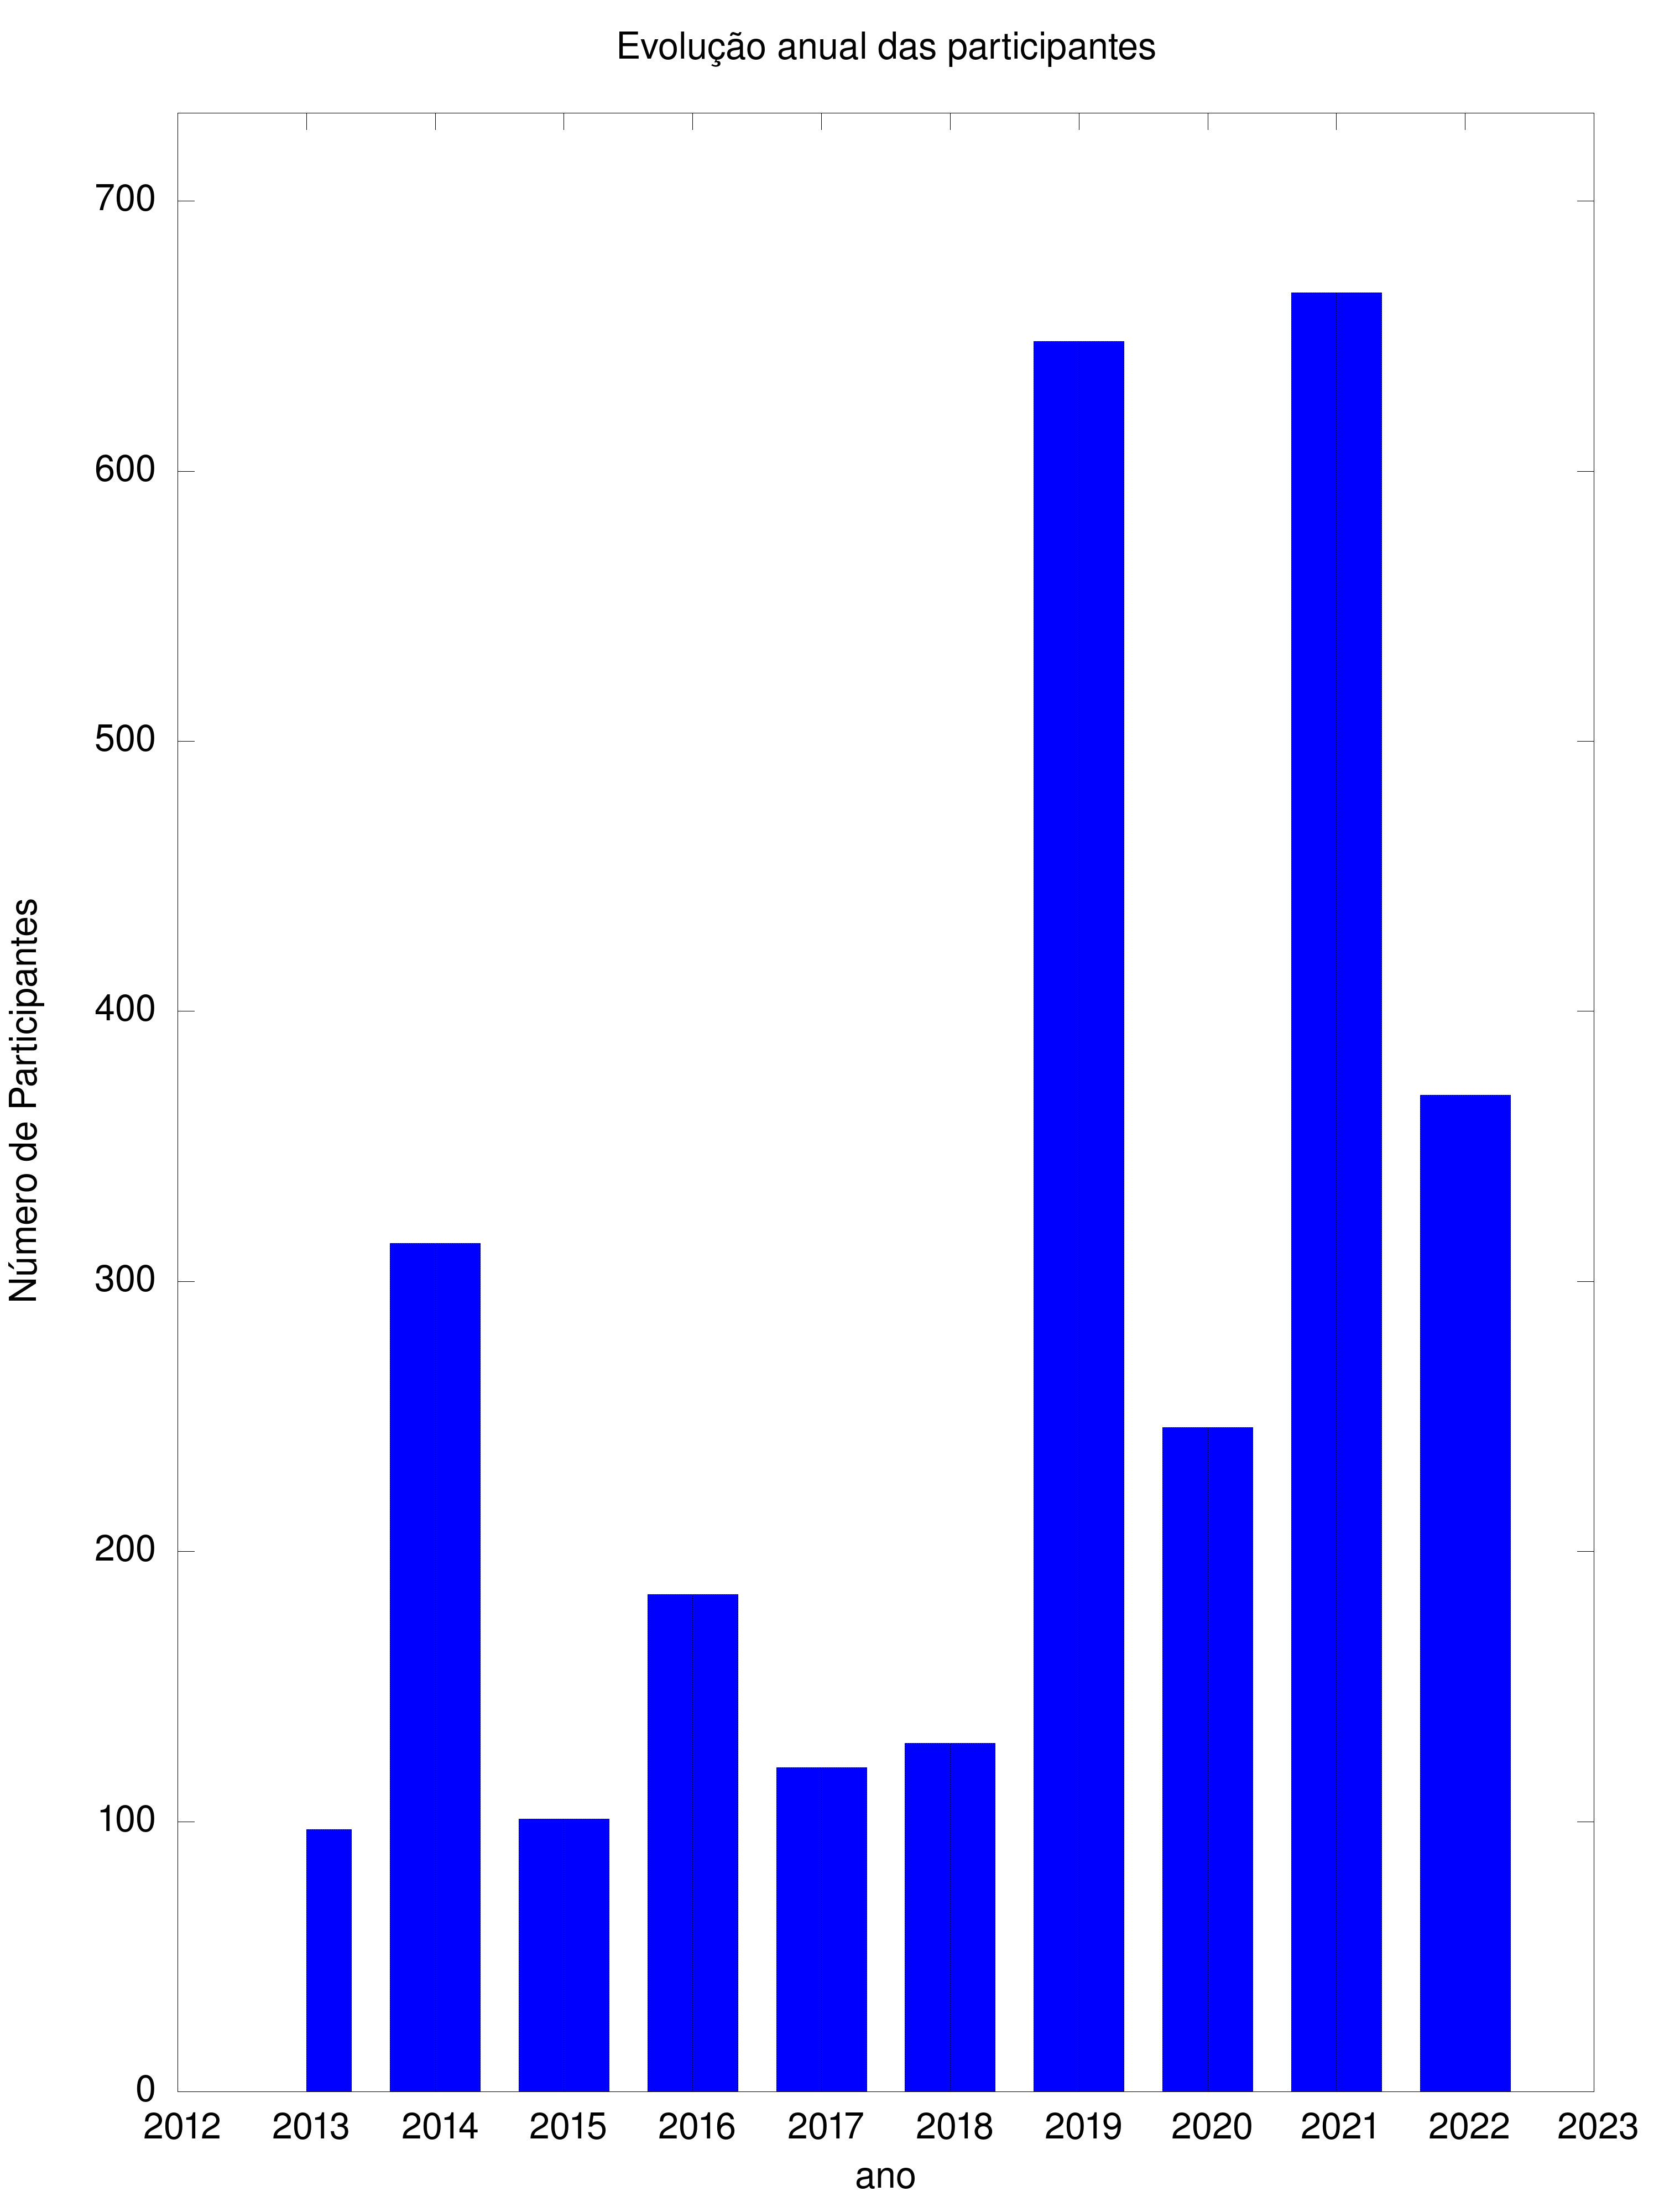
\includegraphics[width=1.0\linewidth]{../../imagens/output-participantes2.jpeg}
                \caption{Evolu\c{c}\~ao anual do n\'umero de participantes individuais.}
                \label{e01eb26f443a577db4a1d382417f8c1bb57ee435}
\end{minipage}
\hspace{0.5cm}
\begin{minipage}[b]{0.4\linewidth}
        \centering
                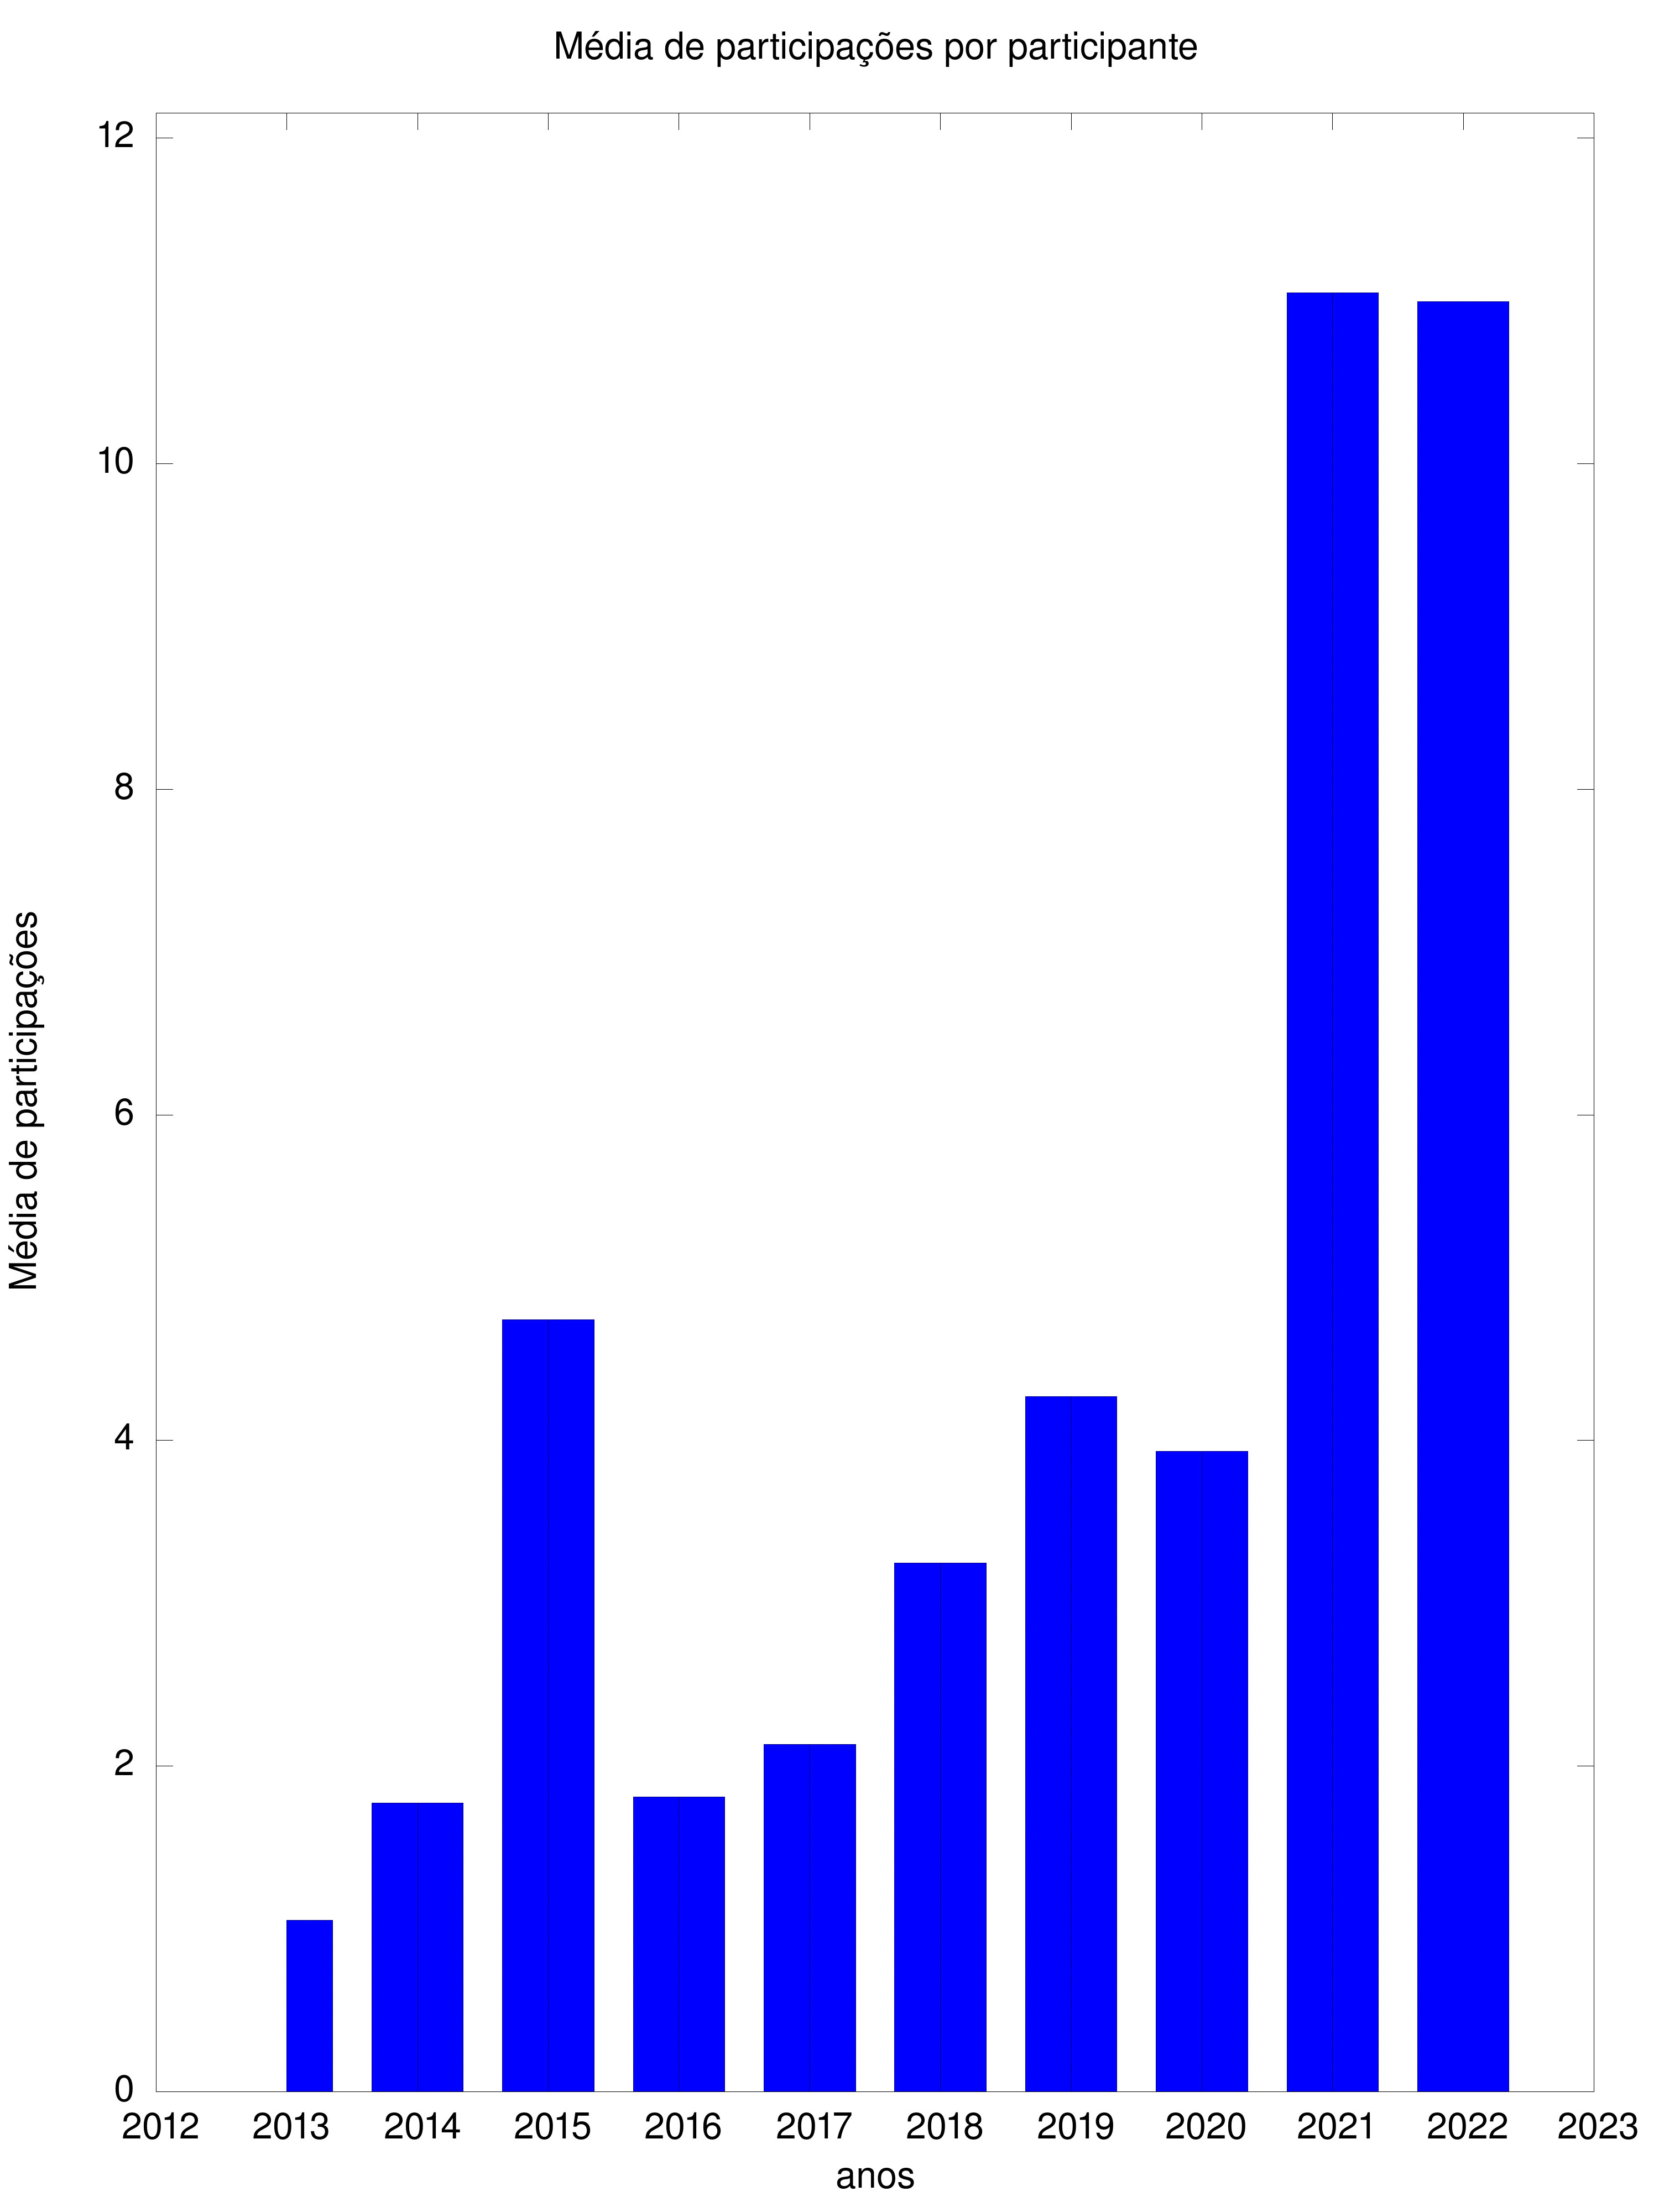
\includegraphics[width=1.0\linewidth]{../../imagens/output-media-participacoes.jpeg}
                \caption{Evolu\c{c}\~ao anual da m\'edia de participa\c{c}\~oes por participante.}
                \label{a8f2d72073b88290f9b8731b144383d2f7c4dc4b}
\end{minipage}%
\hspace{0.5cm}
\end{figure}



\'E importante atentar para uma sutileza: a diferen\c{c}a entre \textquotedbl n\'umero de participantes\textquotedbl  e \textquotedbl n\'umero de participa\c{c}\~oes\textquotedbl .










N\'umero de participantes significa o n\'umero de indiv\'{\i}duos que partiparam de eventos naquele ano, contabilizados uma vez s\'o, mesmo que tenham participado em mais de um evento no mesmo ano.










N\'umero de participa\c{c}\~oes significa o n\'umero de vezes que participantes frequentaram eventos do WASH naquele ano, mesmo que seja contabilizada a mesma pessoa duas ou mais vezes.










Observada essa diferen\c{c}a, o gr\'afico abaixo traz o n\'umero de participantes por ano.










Agora podemos calcular a m\'edia de participa\c{c}\~oes por participante, dividindo, um a um, os dados da evolu\c{c}\~ao anual das participa\c{c}\~oes pela evolu\c{c}\~ao anual dos participantes, como segue.










\subsection[Distribui\c{c}\~ao de partipantes por sexo]{Distribui\c{c}\~ao de partipantes por sexo}\label{Distribui\c{c}\~ao de partipantes por sexo}
Sabe-se que as pessoas do sexo feminino s\~ao particularmente desprivilegiadas quando o tema \'e igualdade de acesso \`as disciplinas de Science, Technology, Engineering 










Por esta raz\~ao, \'e de particular interesse para este trabalho analisar o equil\'{\i}brio no atendimento a participantes do sexo masculino e do sexo feminino.










Mas esta an\'alise, como antecipado no cap\'{\i}tulo de Materiais e M\'etodos, n\~ao foi planejada no in\'{\i}cio do projeto, uma vez que n\~ao havia, h\'a 10 anos atr\'as, a ambi\c{c}\~ao de crescimento que se alcan\c{c}ou.










Esta situa\c{c}\~ao impactou tamb\'em a capacidade do projeto de fazer uma an\'alise mais inclusiva no sentido da identifica\c{c}\~ao de g\^enero dos participantes.










Portanto, na aus\^encia de informa\c{c}\~oes cadastrais mais detalhadas no que se refere \`a auto-declara\c{c}\~ao de g\^enero dos participantes nos primeiros 5 anos do projeto, bem como em face \`a recente resist\^encia de parceiros em fornecer dados, decorrente da LGPD, foi preciso desenvolver um m\'etodo de \textquotedbl estimativa\textquotedbl  do sexo dos participantes com base no primeiro nome dos mesmos.










Este m\'etodo n\~ao tem a finalidade de atribuir um g\^enero aos participantes. O m\'etodo \'e anonimizado de forma que a contabiliza\c{c}\~ao de um participante do sexo feminino e masculino se d\'a num contexto n\~ao personalizado.










De forma sum\'aria pode-se descrever o m\'etodo como uma verifica\c{c}\~ao se o primeiro nome do participante est\'a numa lista extensiva de nomes \textquotedbl considerados masculinos\textquotedbl , situa\c{c}\~ao em que, de forma anonimizada, um contador de participantes masculinos \'e incrementado. Caso o primeiro nome do participante esteja numa lista de nomes \textquotedbl considerados femininos\textquotedbl , o contador de participantes femininos \'e incrementado. Quando o nome n\~ao est\'a em nenhuma das listas, ou quando \'e um nome indefinido, o contador de \textquotedbl sexo desconhecido \'e incrementado\textquotedbl .










Como recentemente, a partir de 2019, foi inclu\'{\i}da na plataforma Platu\'osh a pergunta sobre sexo do participante de forma autodeclarat\'oria, uma parte dos dados \'e fornecida pelos pr\'oprios participantes.










O gr\'afico abaixo mostra a distribui\c{c}\~ao de g\^eneros masculinos, femininos, desconhecidos e outros no universo de participantes do WASH. Nota-se um equil\'{\i}brio entre os participantes, com 49.4\% de mulheres e 48.3\% de homens, havendo ainda 2.1\% de g\^eneros desconhecidos. Apenas 5 cadastros apontam g\^eneros que n\~ao se encaixam nas demais concep\c{c}\~oes.










A afirma\c{c}\~ao de que existe um equil\'{\i}brio \'e de car\'ater amostral e n\~ao absoluto, podendo haver situa\c{c}\~oes em que para determinada faixa et\'aria, um g\^enero prevale\c{c}a sobre o outro.












\captionsetup{format=plain}
\begin{figure}[max size={\textwidth}{\textheight}]

\centering


\begin{minipage}[b]{0.4\linewidth}
        \centering
                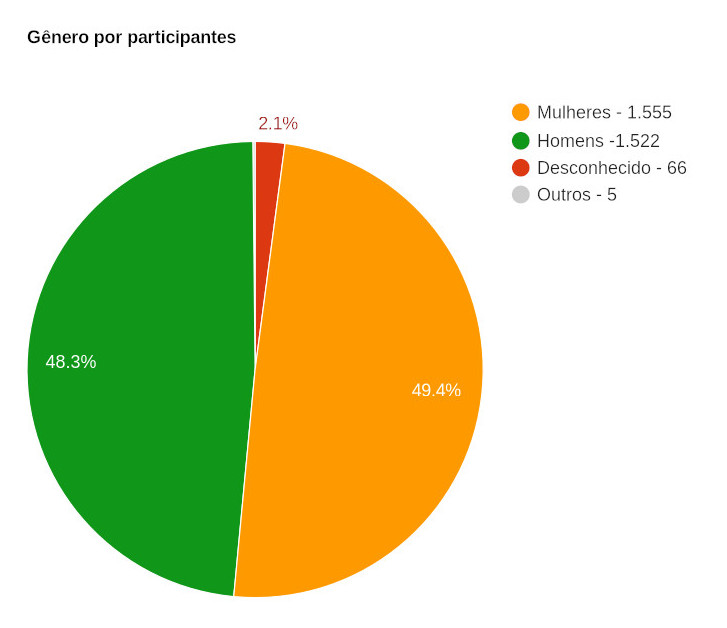
\includegraphics[width=1.0\linewidth]{../../imagens/genero-todos-crop.jpeg}
                \caption{Distribui\c{c}\~ao dos participantes por g\^enero. Esses dados foram obtidos por meio de infer\^encia, a posteriori, utilizando o primeiro nome dos participantes como forma de estimar o percentual de participantes de ambos os g\^eneros.}
                \label{ef11d820efb73d78fb64eb6bdd03853471a8e89f}
\end{minipage}%
\hspace{0.5cm}
\end{figure}



\subsection[N\'umero de Bolsistas]{N\'umero de Bolsistas}\label{N\'umero de Bolsistas}
O m\'etodo do WASH, descrito na Portaria CTI 178/2018, pressup\~oe a atua\c{c}\~ao de bolsistas de inicia\c{c}\~ao cient\'{\i}fica (Bolsas de Fomento do CNPq modalidades ITIA e ITIB) como multiplicadores do projeto. Al\'em disso, o Projeto conta com Bolsistas Extensionistas (Bolsa CNPq EXP), Bolsistas de Apoio T\'ecnico (Bolsa CNPq ATP).1










Desta forma, o n\'umero de bolsistas atuantes no projeto \'e um importante elemento de caracteriza\c{c}\~ao do mesmo para que se conhe\c{c}a:











\begin{alineas}
\item o balan\c{c}o entre o n\'umero de crian\c{c}as e adolescentes atendidos e n\'umero de  bolsistas atuantes no projeto.
\item a produ\c{c}\~ao de resultados cient\'{\i}ficos e de inova\c{c}\~ao, concretizado na forma dos relat\'orios  e entreg\'aveis produzidos pelos bolsistas
\item a relev\^ancia do apoio \`a pesquisa e extens\~ao das entidades promotoras parceiras (Universidades e Centros de Pesquisa)
\end{alineas}

A an\'alise dos dados existentes na base de dados Platu\'osh indica a exist\^encia de 164 bolsistas no Programa WASH. Para obter este n\'umero foi preciso desconsiderar repeti\c{c}\~oes dos registros de afilia\c{c}\~oes (tabela \textquotedbl afiliacoes\textquotedbl  da base de dados).










Mas a experi\^encia desta candidata no apoio \`a implementa\c{c}\~ao de bolsas no \^ambito do Programa WASH indicava a percep\c{c}\~ao de um n\'umero muito maior de bolsistas.










Esta intui\c{c}\~ao de que o n\'umero de bolsistas deveria ser muito maior do que o fornecido pela afilia\c{c}\~ao dos participantes registrada na Platu\'osh acendeu um sinal vermelho.










Estava claro que o registro de afilia\c{c}\~oes da Platu\'osh n\~ao era a forma mais adequada de saber quantos bolsistas passaram pelo projeto.





















Uma pondera\c{c}\~ao sobre os motivos desta inadequa\c{c}\~ao levaram ao seguinte conjunto de reflex\~oes:











\begin{alineas}
\item a plataforma Platu\'osh \'e uma ferramenta dispon\'{\i}vel apenas a partir de 2018, raz\~ao pela qual n\~ao cobre todo o per\'{\i}odo de exist\^encia do projeto.
\item a plataforma Platu\'osh foi originalmente concebida para registro de presen\c{c}a e testemunho de realiza\c{c}\~ao de eventos, para fins de presta\c{c}\~ao de contas aos \'org\~aos de fomento, n\~ao havendo, inicialmente, a inten\c{c}\~ao de registrar os bolsistas
\item assim que a plataforma Platu\'osh foi adaptada para o registro de bolsistas, houve um esfor\c{c}o de recupera\c{c}\~ao de dados pregressos, mas este trabalho ficou naturalmente incompleto, pelo r\'apido crescimento do projeto, havendo um persistente back-log de dados de bolsistas (ac\'umulo de trabalho atrasado).
\item recentemente o preenchimento dos cadastros ficou a cargo dos pr\'oprios bolsistas, que ganharam \textquotedbl contas\textquotedbl  na plataforma. Este procedimento \'e naturalmente impreciso, porque muitos bolsistas n\~ao tem pr\'atica em seu preenchimento, apesar dos esfor\c{c}os de capacita\c{c}\~ao da Frente Multiplicadora do WASH
\item existe uma complac\^encia por parte dos bolsistas, que n\~ao preenchem a plataforma como solicitado
\end{alineas}

Consultando a equipe de TI sobre estes problemas com o registro de bolsistas na Platu\'osh, fomos informados que uma tabela auxiliar de registro de bolsistas tinha sido integrada \`a base de dados original. Esta tabela foi denominada \textquotedbl bolsa-cnpq\textquotedbl .










Uma consulta \`a base, utilizando o m\'etodo SQL, levou a um total de 235 registros na tabela \textquotedbl bolsa-cnpq\textquotedbl . Mas uma inspe\c{c}\~ao mais cuidadosa indicou que esta tabela continha todas as concess\~oes de bolsas, com a possibilidade de um bolsista ser contemplado por duas concess\~oes consecutivas, decorrentes da renova\c{c}\~ao de bolsas. Portanto, o n\'umero de 235 bolsistas estava claramente superestimado.










O pr\'oximo passo foi excluir as repeti\c{c}\~oes, agrupando os resultados por bolsista. Com esse m\'etodo chegou-se ao n\'umero de 206 bolsistas.










Esta variabilidade nos dados gerou-nos uma inseguran\c{c}a em rela\c{c}\~ao \`a plataforma Platu\'osh no que tange exclusivamente aos dados de bolsistas.










Assim, sentimo-nos motivados a buscar uma solu\c{c}\~ao independente para o levantamento de dados de bolsas, uma vez que o v\'{\i}nculo dos bolsistas com o CNPq \'e formal e ocorre mediante Termo de Outorga, havendo meios de obter dados absolutos e n\~ao-amostrais.










Contando com o apoio do Coordenador do Programa WASH, foi poss\'{\i}vel levantar a quantidade de bolsistas e a distribui\c{c}\~ao por tipo de bolsas usando a Plataforma Carlos Chagas. Os dados foram obtidos de forma anonimizada pelo coordenador.










Para esse levantamento n\~ao foi utilizada a modelagem de banco de dados relacional, mas simplesmente a tabula\c{c}\~ao em planilhas eletr\^onicas, tecnologia mais acess\'{\i}vel a esta candidata. Desta forma o trabalho pode ser conduzido independentemente do apoio da equipe de TI, podendo, posteriormente, ser utilizado como balizador para melhoria dos processos de coleta de dados de bolsistas no \^ambito do Programa WASH.










\subsection[Caracteriza\c{c}\~ao dos Planos de Trabalhos e Relat\'orios]{Caracteriza\c{c}\~ao dos Planos de Trabalhos e Relat\'orios}\label{Caracteriza\c{c}\~ao dos Planos de Trabalhos e Relat\'orios}
Ao receber o termo de outorga de uma bolsa pelo CNPq, o (a) bolsista assume o compromisso de realizar um projeto de pesquisa, al\'em das atividades de extens\~ao. Estas \'ultimas envolvem a participa\c{c}\~ao como multiplicadores nas oficinas em escolas de ensino fundamental.










As atividades e as entregas referentes ao projeto de pesquisa s\~ao especificadas por meio de um plano de trabalho. Dentre as entregas definidas nesse Plano de Trabalho, \'e obrigat\'orio constar o Relat\'orio, que \'e uma forma de documenta\c{c}\~ao cient\'{\i}fica que segue a mesma estrutura definida no primeiro cap\'{\i}tulo desta disserta\c{c}\~ao.











Assim, uma aspecto importante da caracteriza\c{c}\~ao do Programa WASH \'e contabiliza\c{c}\~ao e classifica\c{c}\~ao dos Planos de Trabalho e Relat\'orios produzidos pelos bolsistas do projeto.










Para a contabiliza\c{c}\~ao dos Planos de Trabalho e dos Relat\'orios produzidos pelos bolsistas foram empregados neste trabalho os seguintes instrumentos:











\begin{alineas}
\item plataforma Platu\'osh, que tem um car\'ater amostral e n\~ao exaustivo em termos de coleta de dados
\item o planejamento e caracteriza\c{c}\~ao financeira do projeto, que \'e um instrumento de compliance do projeto, mas que tamb\'em pode ser utilizado para suprir informa\c{c}\~oes sobre a documenta\c{c}\~ao presente no projeto
\item e o levantamento espec\'{\i}fico conduzido por esta candidata, com base em dados objetivos da Plataforma Carlos Chagas do CNPq, a fonte mais confi\'avel de dados para esse tipo de caracteriza\c{c}\~ao.
\end{alineas}

\subsection[Distribui\c{c}\~ao de temas em relat\'orios]{Distribui\c{c}\~ao de temas em relat\'orios}\label{Distribui\c{c}\~ao de temas em relat\'orios}
participantes










\subsection[N\'umero de oficinas realizadas]{N\'umero de oficinas realizadas}\label{N\'umero de oficinas realizadas}
A evolu\c{c}\~ao do n\'umero de eventos realizados ao longo dos dez anos de exist\^encia do projeto pode ser verificada no gr\'afico abaixo.












\captionsetup{format=plain}
\begin{figure}[htb]

	\begin{center}

		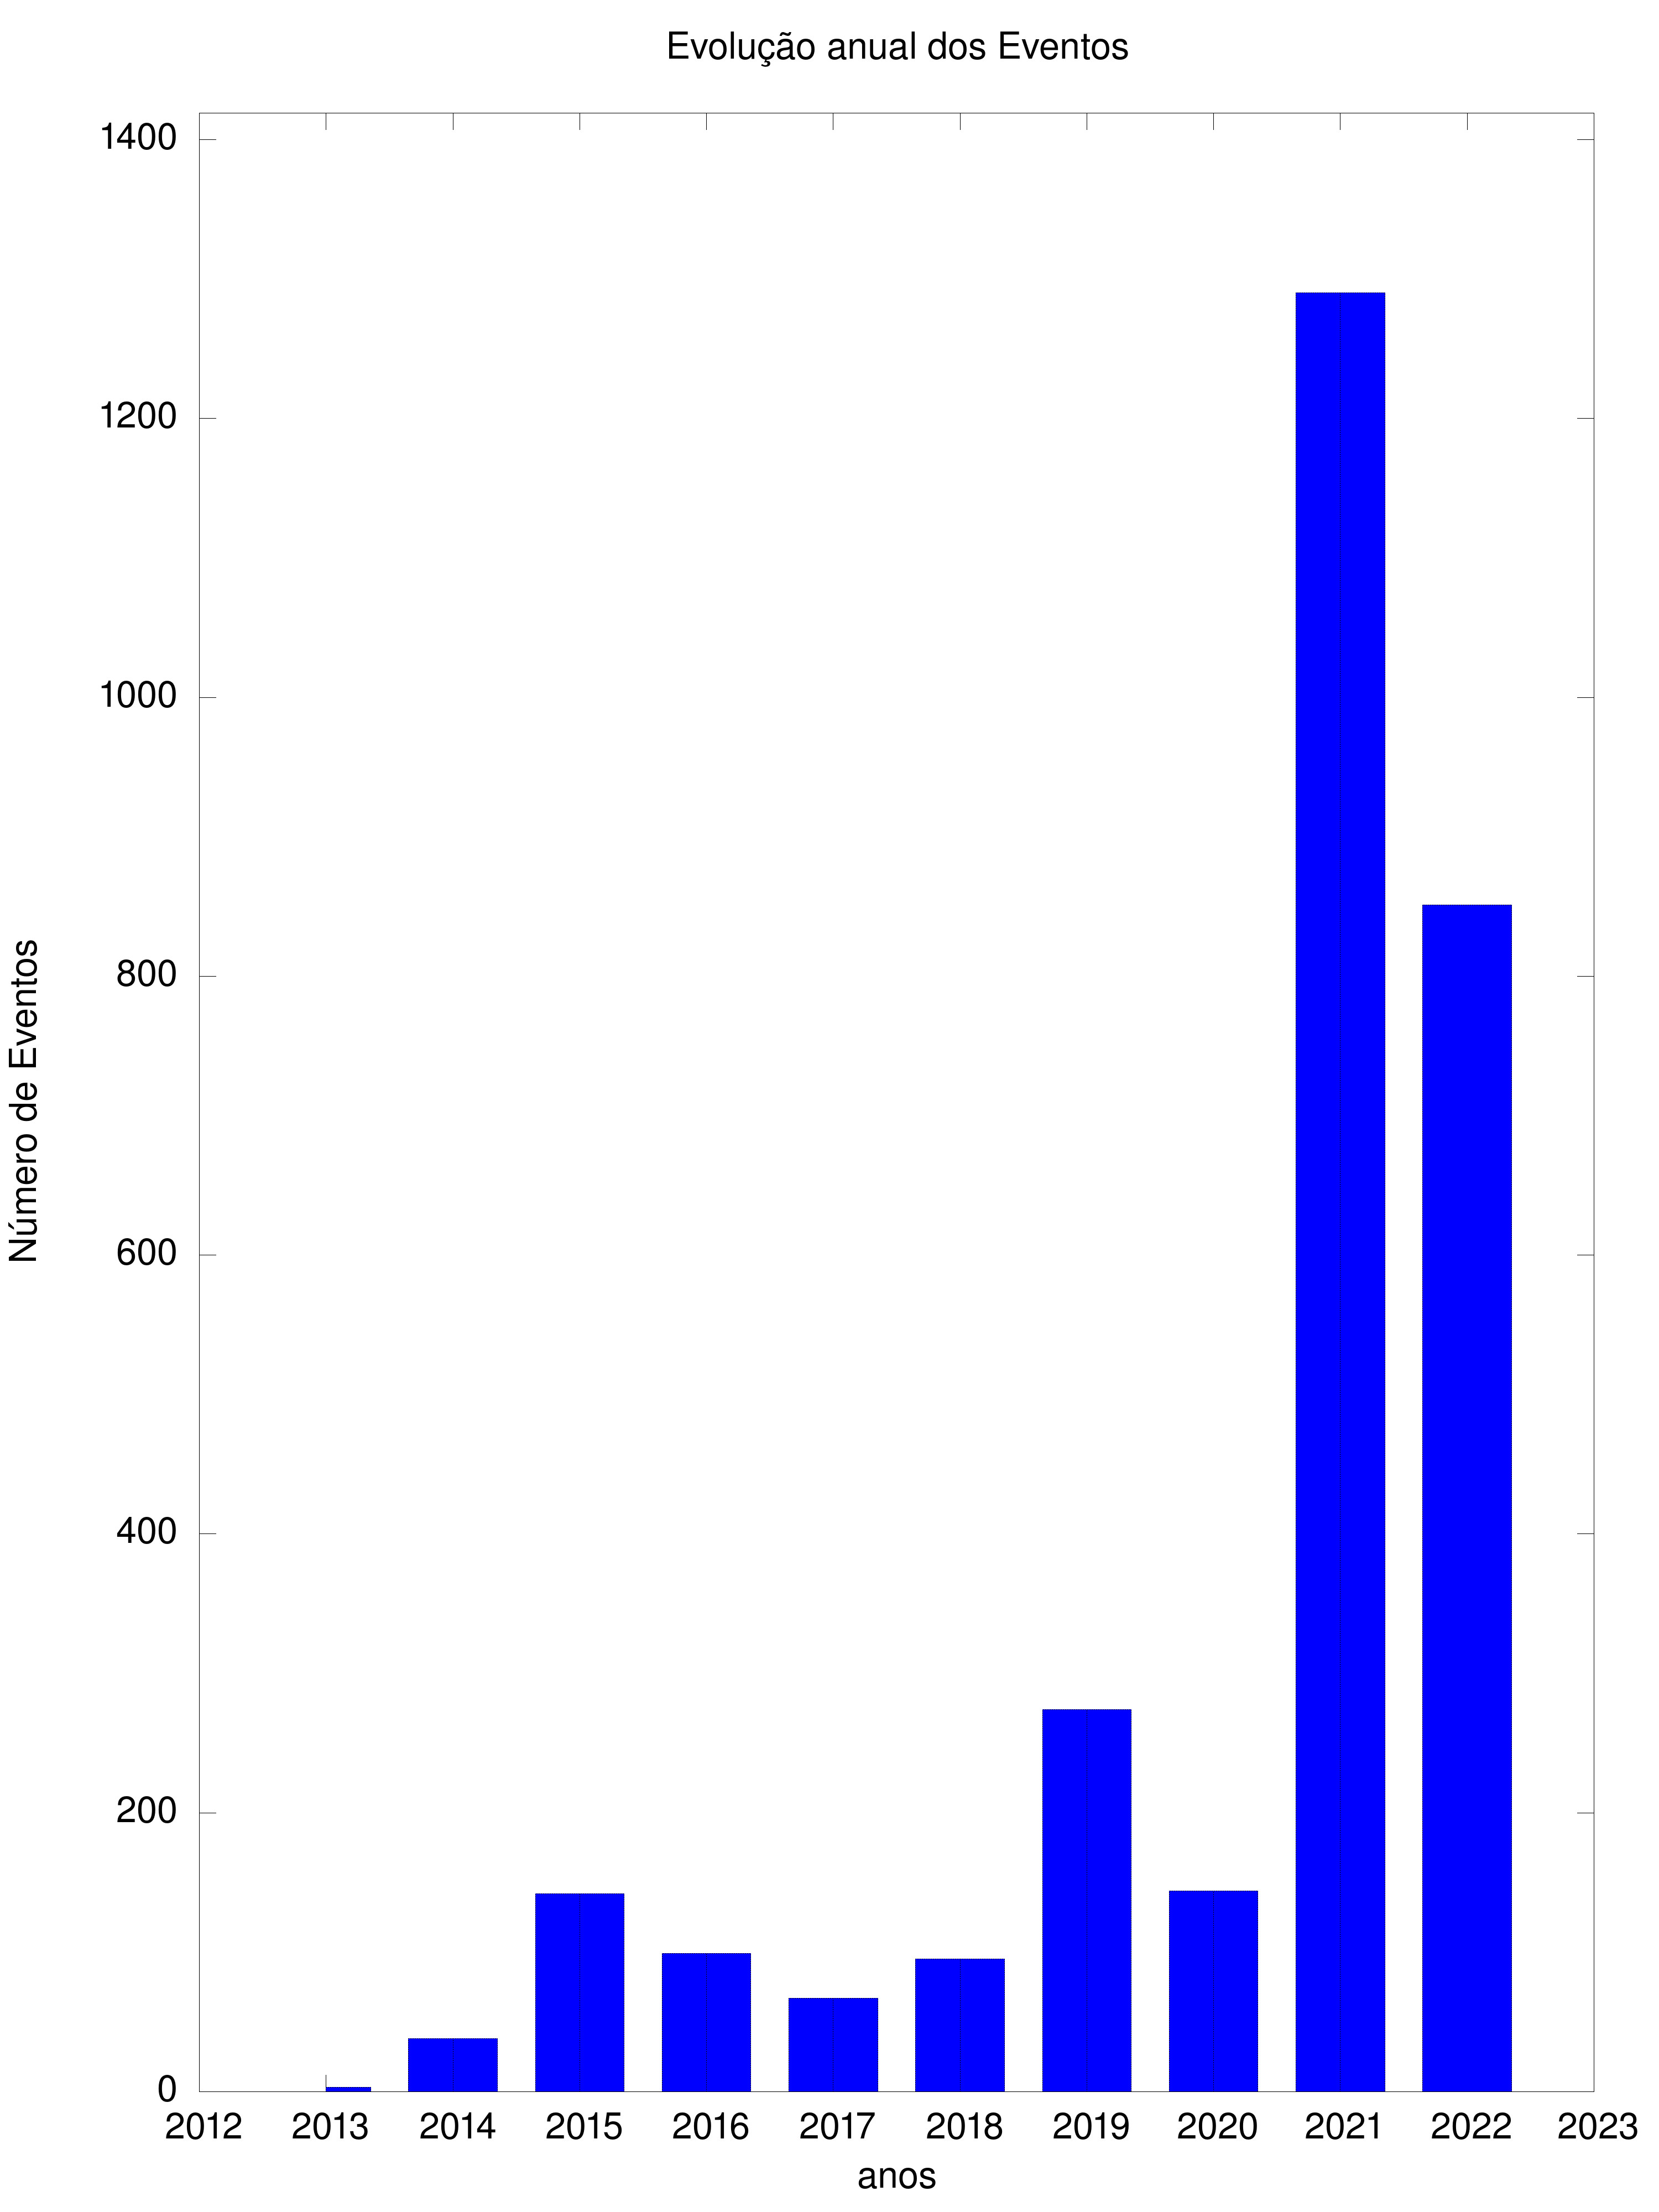
\includegraphics[max size={\textwidth}{\textheight}]{../../imagens/output-eventos.jpeg}

	\end{center}

	\caption{\label{8af5236ba8f91623157f8f95ae10366b416d6049}Evolu\c{c}\~ao anual do n\'umero de oficinas realizadas.}

\end{figure}

\subsection[Distribui\c{c}\~ao et\'aria nas oficinas]{Distribui\c{c}\~ao et\'aria nas oficinas}\label{Distribui\c{c}\~ao et\'aria nas oficinas}
participantes












\captionsetup{format=plain}
\begin{figure}[htb]

	\begin{center}

		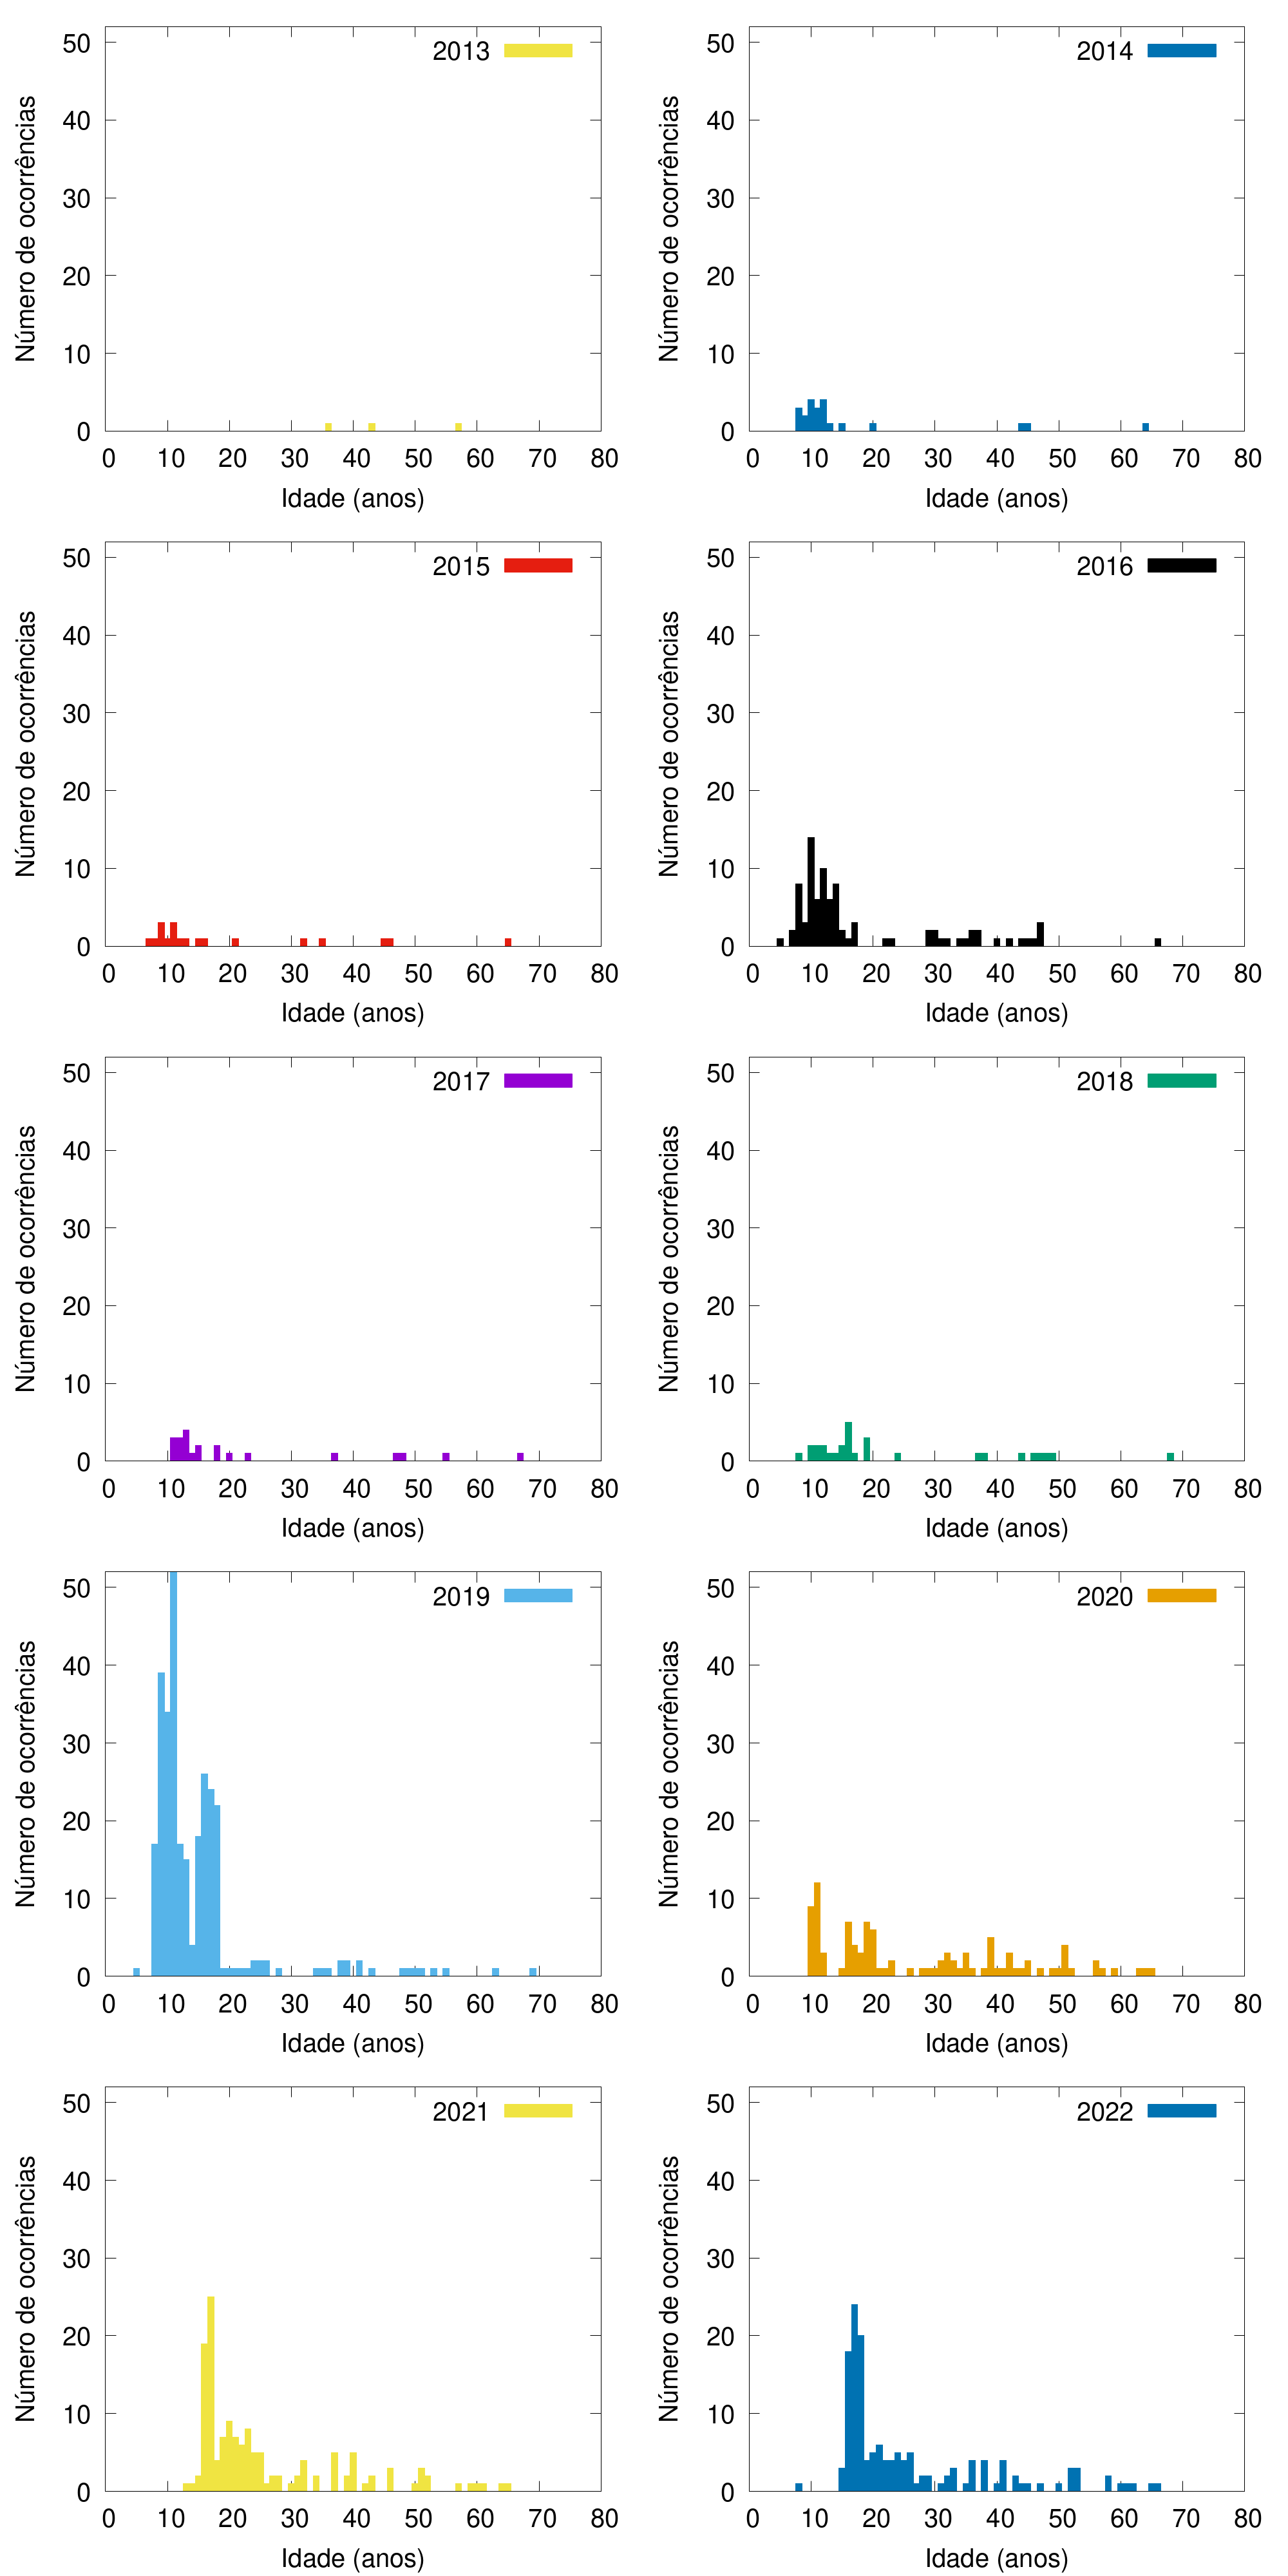
\includegraphics[max size={\textwidth}{\textheight}]{../../imagens/histograma-de-idades-no-ano-do-evento.png}

	\end{center}

	\caption{\label{978341992d3d49498d48c41acc77f05f08f49ead}Distribui\c{c}\~ao et\'aria dos participantes, ano a ano.}

\end{figure}

\subsection[Distribui\c{c}\~ao de temas nas oficinas]{Distribui\c{c}\~ao de temas nas oficinas}\label{Distribui\c{c}\~ao de temas nas oficinas}
participantes










\subsection[Tipos de Atividades realizadas nas oficinas]{Tipos de Atividades realizadas nas oficinas}\label{Tipos de Atividades realizadas nas oficinas}
Primeiro par\'agrafo.










Primeiro par\'agrafo.










Primeiro par\'agrafo.










Primeiro par\'agrafo.










Primeiro par\'agrafo.










Primeiro par\'agrafo.










Primeiro par\'agrafo.










Primeiro par\'agrafo.










\subsection[Cidades Atendidas]{Cidades Atendidas}\label{Cidades Atendidas}
teste










\subsection[Participantes mais ass\'{\i}duos]{Participantes mais ass\'{\i}duos}\label{Participantes mais ass\'{\i}duos}
primeiro par\'agrafo










\section[S\'{\i}ntese anal\'{\i}tica dos 3 eixos]{S\'{\i}ntese anal\'{\i}tica dos 3 eixos}\label{S\'{\i}ntese anal\'{\i}tica dos 3 eixos}
Aqui ser\'a feita a s\'{\i}ntese das 3 dimens\~oes.










\chapter[CONCLUS\~OES]{CONCLUS\~OES}\label{CONCLUS\~OES}
Foi poss\'{\i}vel realizar a caracteriza\c{c}\~ao e a modelagem nos 3 eixos indicados, o que permitiu verificar as hip\'oteses levantadas, como segue:










\chapter[PRODUTOS TECNOL\'OGICOS]{PRODUTOS TECNOL\'OGICOS}\label{PRODUTOS TECNOL\'OGICOS}
Este trabalho gerou v\'arios produtos tecnol\'ogicos que s\~ao descritos a seguir.










\section[V\'{\i}deo/Entrevista: Papert e Afira Ripper]{V\'{\i}deo/Entrevista: Papert e Afira Ripper}\label{V\'{\i}deo/Entrevista: Papert e Afira Ripper}
A entrevista com a Profa. Afira Ripper foi transformada em \'audio-visual, estando dispon\'{\i}vel para o p\'ublico por meio dos links:











\begin{alineas}
\item Parte 1: https://www.youtube.com/watch?v=fMsy7eW8vxU
\item Parte 2: https://www.youtube.com/watch?v=inxixL5iK4I
\end{alineas}

\section[Revis\~ao do documento de refer\^encia do Programa WASH]{Revis\~ao do documento de refer\^encia do Programa WASH}\label{Revis\~ao do documento de refer\^encia do Programa WASH}
Este produto educacional tem por objetivo apresentar, ap\'os anos de pr\'atica e de valida\c{c}\~ao do m\'etodo WASH, uma vers\~ao atualizada do Documento de Refer\^encia constante na Portaria nº 178/2018/SEI-CTI, de 12 de novembro de 2018.










Esta revis\~ao teve, como finalidade:











\begin{alineas}
\item melhorar as condi\c{c}\~oes de dissemina\c{c}\~ao da pr\'atica do WASH, ampliando sua ado\c{c}\~ao por escolas p\'ublicas
\item contribuir com a dissemina\c{c}\~ao do m\'etodo cient\'{\i}fico, facilitando o acesso a atividades de turno e contra-turno voltadas para STEAM
\item adaptar o Programa WASH a situa\c{c}\~oes de isolamento social, prevendo atividades remotas
\end{alineas}

Identificamos esta necessidade de revis\~ao porque, ao longo dos 09 de execu\c{c}\~ao do WASH, observamos um crescente interesse, por parte de outras institui\c{c}\~oes, pela reprodu\c{c}\~ao do Programa WASH.










\chapter[REFER\^ENCIAS]{REFER\^ENCIAS}\label{REFER\^ENCIAS}
\begin{flushleft}
\begin{flushleft}
\begin{flushleft}
\begin{flushleft}
\begin{flushleft}
\begin{flushleft}
\begin{flushleft}
\begin{flushleft}
\begin{flushleft}
\begin{flushleft}
[MEO, 2018] Meo, S.A. Anatomy and physiology of a scientific paper, Saudi Journal of Biological Sciences, V.25, I.7, November 2018, Pg. 1278-1283
\end{flushleft}


\end{flushleft}


\end{flushleft}


\end{flushleft}


\end{flushleft}


\end{flushleft}


\end{flushleft}


\end{flushleft}


\end{flushleft}


\end{flushleft}


\begin{flushleft}
\begin{flushleft}
\begin{flushleft}
\begin{flushleft}
\begin{flushleft}
\begin{flushleft}
\begin{flushleft}
\begin{flushleft}
\begin{flushleft}
\begin{flushleft}
[LEVY, 2000] LEVY, P. Cibercultura. 2 ed. Editora 34,  Rio de Janeiro:, 2000.p. 14 e 15.
\end{flushleft}


\end{flushleft}


\end{flushleft}


\end{flushleft}


\end{flushleft}


\end{flushleft}


\end{flushleft}


\end{flushleft}


\end{flushleft}


\end{flushleft}


\begin{flushleft}
\begin{flushleft}
\begin{flushleft}
\begin{flushleft}
\begin{flushleft}
\begin{flushleft}
\begin{flushleft}
\begin{flushleft}
\begin{flushleft}
\begin{flushleft}
[DANTAS, 1988] DANTAS, V. Guerrilha Tecnol\'ogica, Livros T\'ecnicos e Cient\'{\i}ficos, janeiro de 1988
\end{flushleft}


\end{flushleft}


\end{flushleft}


\end{flushleft}


\end{flushleft}


\end{flushleft}


\end{flushleft}


\end{flushleft}


\end{flushleft}


\end{flushleft}


\begin{flushleft}
\begin{flushleft}
\begin{flushleft}
\begin{flushleft}
\begin{flushleft}
\begin{flushleft}
\begin{flushleft}
\begin{flushleft}
\begin{flushleft}
\begin{flushleft}
[DUTTON, 2004] DUTTON, W. Social Transformation in an Information Society: Rethinking Access to You and the World, UNESCO 2004, Society: Rethinking Access to You and the World, 
\end{flushleft}


\end{flushleft}


\end{flushleft}


\end{flushleft}


\end{flushleft}


\end{flushleft}


\end{flushleft}


\end{flushleft}


\end{flushleft}


\end{flushleft}


\begin{flushleft}
\begin{flushleft}
\begin{flushleft}
\begin{flushleft}
\begin{flushleft}
\begin{flushleft}
\begin{flushleft}
\begin{flushleft}
\begin{flushleft}
\begin{flushleft}
[HARARI, 2018]  HARARI, Y. 21 Li\c{c}\~oes para o s\'eculo 21, Companhia das Letras, 2018
\end{flushleft}


\end{flushleft}


\end{flushleft}


\end{flushleft}


\end{flushleft}


\end{flushleft}


\end{flushleft}


\end{flushleft}


\end{flushleft}


\end{flushleft}


\begin{flushleft}
\begin{flushleft}
\begin{flushleft}
\begin{flushleft}
\begin{flushleft}
\begin{flushleft}
\begin{flushleft}
\begin{flushleft}
\begin{flushleft}
\begin{flushleft}
[BATES, 2014] BATES COLLEGE, How to Write a Paper in Scientific Journal Style and Format, v.10-2014, acessado em: https://www.bates.edu/biology/files/2010/06/How-to-Write-Guide-v10-2014.pdf, 2022
\end{flushleft}


\end{flushleft}


\end{flushleft}


\end{flushleft}


\end{flushleft}


\end{flushleft}


\end{flushleft}


\end{flushleft}


\end{flushleft}


\end{flushleft}


\begin{flushleft}
\begin{flushleft}
\begin{flushleft}
\begin{flushleft}
\begin{flushleft}
\begin{flushleft}
\begin{flushleft}
\begin{flushleft}
\begin{flushleft}
\begin{flushleft}
[KARA-JUNIOR, 2014] KARA-JUNIOR, N. Estrutura, estilo e escrita de artigo cient\'{\i}fico: a maneira com que pesquisadores reconhecem seus pares, Revista Brasileira de Oftalmologia 73(5), Set-Out 2014.
\end{flushleft}


\end{flushleft}


\end{flushleft}


\end{flushleft}


\end{flushleft}


\end{flushleft}


\end{flushleft}


\end{flushleft}


\end{flushleft}


\end{flushleft}


\begin{flushleft}
\begin{flushleft}
\begin{flushleft}
\begin{flushleft}
\begin{flushleft}
\begin{flushleft}
\begin{flushleft}
\begin{flushleft}
\begin{flushleft}
\begin{flushleft}
[MAMMANA, 2019] MAMMANA, A.P. Documenta\c{c}\~ao Cient\'{\i}fica, acessado no Youtube em 2022
\end{flushleft}


\end{flushleft}


\end{flushleft}


\end{flushleft}


\end{flushleft}


\end{flushleft}


\end{flushleft}


\end{flushleft}


\end{flushleft}


\end{flushleft}


\begin{flushleft}
\begin{flushleft}
\begin{flushleft}
\begin{flushleft}
\begin{flushleft}
\begin{flushleft}
\begin{flushleft}
\begin{flushleft}
\begin{flushleft}
\begin{flushleft}
[CATTERALL, 2017] CATTERALL, L.G. A brief history of STEM and STEAM from an Inadvertent Insider, The STEAM Journal, V 3(1) 2017
\end{flushleft}


\end{flushleft}


\end{flushleft}


\end{flushleft}


\end{flushleft}


\end{flushleft}


\end{flushleft}


\end{flushleft}


\end{flushleft}


\end{flushleft}


\begin{flushleft}
\begin{flushleft}
\begin{flushleft}
\begin{flushleft}
\begin{flushleft}
\begin{flushleft}
\begin{flushleft}
\begin{flushleft}
\begin{flushleft}
\begin{flushleft}
[ENGLEBART, 2017] ENGLEBART, D. Microeletronics and the art of similitude, 1960 IEEE International Solid-State Circuits Conference. Digest of Technical Papers, 10-12 de fevereiro de 1960
\end{flushleft}


\end{flushleft}


\end{flushleft}


\end{flushleft}


\end{flushleft}


\end{flushleft}


\end{flushleft}


\end{flushleft}


\end{flushleft}


\end{flushleft}


\begin{flushleft}
\begin{flushleft}
\begin{flushleft}
\begin{flushleft}
\begin{flushleft}
\begin{flushleft}
\begin{flushleft}
\begin{flushleft}
\begin{flushleft}
\begin{flushleft}
[NEGROPONTE, 2004] NEGROPONTE, N. Brazil's Plan 2004, acervo pessoal de Victor Mammana
\end{flushleft}


\end{flushleft}


\end{flushleft}


\end{flushleft}


\end{flushleft}


\end{flushleft}


\end{flushleft}


\end{flushleft}


\end{flushleft}


\end{flushleft}


\begin{flushleft}
\begin{flushleft}
\begin{flushleft}
\begin{flushleft}
\begin{flushleft}
\begin{flushleft}
\begin{flushleft}
\begin{flushleft}
\begin{flushleft}
\begin{flushleft}
[PAPERT, 2005] PAPERT, S. (2005). Teaching Children Thinking. Contemporary Issues in Technology and Teacher Education, 5(3), 353-365. Waynesville, NC USA: Society for Information Technology \& Teacher Education. Retrieved July 26, 2022
\end{flushleft}


\end{flushleft}


\end{flushleft}


\end{flushleft}


\end{flushleft}


\end{flushleft}


\end{flushleft}


\end{flushleft}


\end{flushleft}


\end{flushleft}


\begin{flushleft}
\begin{flushleft}
\begin{flushleft}
\begin{flushleft}
\begin{flushleft}
\begin{flushleft}
\begin{flushleft}
\begin{flushleft}
\begin{flushleft}
\begin{flushleft}
[MAMMANA e TOZZI, 2018] Avalia\c{c}\~ao do Programa OLPC, Cubat\~ao 2018
\end{flushleft}


\end{flushleft}


\end{flushleft}


\end{flushleft}


\end{flushleft}


\end{flushleft}


\end{flushleft}


\end{flushleft}


\end{flushleft}


\end{flushleft}


\begin{flushleft}
\begin{flushleft}
\begin{flushleft}
\begin{flushleft}
\begin{flushleft}
\begin{flushleft}
\begin{flushleft}
\begin{flushleft}
\begin{flushleft}
\begin{flushleft}
[BELL, 1973]  BELL, 1973, professor de Harvard, que a partir do texto The Coming of Post Industrial Society [XXX BELL, Daniel. The Coming of Post-industrial Society. Nova York: Basic Books, 1973
\end{flushleft}


\end{flushleft}


\end{flushleft}


\end{flushleft}


\end{flushleft}


\end{flushleft}


\end{flushleft}


\end{flushleft}


\end{flushleft}


\end{flushleft}


\begin{flushleft}
\begin{flushleft}
\begin{flushleft}
\begin{flushleft}
\begin{flushleft}
\begin{flushleft}
\begin{flushleft}
\begin{flushleft}
\begin{flushleft}
\begin{flushleft}
[MAMMANA, 2020] MAMMANA, A. Semin\'ario - Documenta\c{c}\~ao em Ci\^encia e Tecnologia, v\'{\i}deo do Youtube, https://www.youtube.com/watch?v=-ek\_EjIDWnE acessado em 12/08/2022
\end{flushleft}


\end{flushleft}


\end{flushleft}


\end{flushleft}


\end{flushleft}


\end{flushleft}


\end{flushleft}


\end{flushleft}


\end{flushleft}


\end{flushleft}


\begin{flushleft}
\begin{flushleft}
\begin{flushleft}
\begin{flushleft}
\begin{flushleft}
\begin{flushleft}
\begin{flushleft}
\begin{flushleft}
\begin{flushleft}
\begin{flushleft}
[CTI, 2018] Portaria CTI 178/2018.
\end{flushleft}


\end{flushleft}


\end{flushleft}


\end{flushleft}


\end{flushleft}


\end{flushleft}


\end{flushleft}


\end{flushleft}


\end{flushleft}


\end{flushleft}


\begin{flushleft}
\begin{flushleft}
\begin{flushleft}
\begin{flushleft}
\begin{flushleft}
\begin{flushleft}
\begin{flushleft}
\begin{flushleft}
\begin{flushleft}
\begin{flushleft}
[CGEE, 2010] Avalia\c{c}\~ao do PIDs
\end{flushleft}


\end{flushleft}


\end{flushleft}


\end{flushleft}


\end{flushleft}


\end{flushleft}


\end{flushleft}


\end{flushleft}


\end{flushleft}


\end{flushleft}


\begin{flushleft}
\begin{flushleft}
\begin{flushleft}
\begin{flushleft}
\begin{flushleft}
\begin{flushleft}
\begin{flushleft}
\begin{flushleft}
\begin{flushleft}
\begin{flushleft}
[Marczal, 2016] Marczal, E. S. Introdu\c{c}\~ao \`a historiografia: da abordagem tradicional \`as perspectivas p\'os-modernas. Curitiba: Intersaberes, 2016, 1a Edi\c{c}\~ao.
\end{flushleft}


\end{flushleft}


\end{flushleft}


\end{flushleft}


\end{flushleft}


\end{flushleft}


\end{flushleft}


\end{flushleft}


\end{flushleft}


\end{flushleft}


\begin{flushleft}
\begin{flushleft}
\begin{flushleft}
\begin{flushleft}
\begin{flushleft}
\begin{flushleft}
\begin{flushleft}
\begin{flushleft}
\begin{flushleft}
\begin{flushleft}
[FREITAS, 2019] FREITAS, I. TEORIAS DA HIST\'ORIA NA HISTORIOGRAFIA DE RANKE, Ponta de Lan\c{c}a, S\~ao Crist\'ov\~ao, v. 13, n. 25, jul. - dez. 2019.
\end{flushleft}


\end{flushleft}


\end{flushleft}


\end{flushleft}


\end{flushleft}


\end{flushleft}


\end{flushleft}


\end{flushleft}


\end{flushleft}


\end{flushleft}


\begin{flushleft}
\begin{flushleft}
\begin{flushleft}
\begin{flushleft}
\begin{flushleft}
\begin{flushleft}
\begin{flushleft}
\begin{flushleft}
\begin{flushleft}
\begin{flushleft}
[WIKIPEDIA, 2022] Imagem obtida da WIKIPEDIA acessada em 17 de agosto de 2022, atrav\'es da URL https://pt.wikipedia.org/wiki/Her\'odoto
\end{flushleft}


\end{flushleft}


\end{flushleft}


\end{flushleft}


\end{flushleft}


\end{flushleft}


\end{flushleft}


\end{flushleft}


\end{flushleft}


\end{flushleft}


\begin{flushleft}
\begin{flushleft}
\begin{flushleft}
\begin{flushleft}
\begin{flushleft}
\begin{flushleft}
\begin{flushleft}
\begin{flushleft}
\begin{flushleft}
\begin{flushleft}
[BENTIVOGLIO, 2010] BENTIVOGLIO, J. Hist\'oria e narrativa na Historiografia alem\~a do s\'eculo XIX Anos 90, Porto Alegre, v. 17, n. 32, p.185-218, dez. 2010
\end{flushleft}


\end{flushleft}


\end{flushleft}


\end{flushleft}


\end{flushleft}


\end{flushleft}


\end{flushleft}


\end{flushleft}


\end{flushleft}


\end{flushleft}


\begin{flushleft}
\begin{flushleft}
\begin{flushleft}
\begin{flushleft}
\begin{flushleft}
\begin{flushleft}
\begin{flushleft}
\begin{flushleft}
\begin{flushleft}
\begin{flushleft}
[TEIXEIRA, 2008] TEIXEIRA, F.C. Uma constru\c{c}\~ao de fatos e palavras: C\'{\i}cero e a concep\c{c}\~ao ret\'orica da hist\'oria, VARIA HISTORIA, Belo Horizonte, vol. 24, nº 40: p.551-568, jul/dez 2008
\end{flushleft}


\end{flushleft}


\end{flushleft}


\end{flushleft}


\end{flushleft}


\end{flushleft}


\end{flushleft}


\end{flushleft}


\end{flushleft}


\end{flushleft}


\begin{flushleft}
\begin{flushleft}
\begin{flushleft}
\begin{flushleft}
\begin{flushleft}
\begin{flushleft}
\begin{flushleft}
\begin{flushleft}
\begin{flushleft}
\begin{flushleft}
[Setzer e Silva, 2017] Setzer, V. W.; Silva, F. S. C. Banco de Dados - Aprenda o que s\~ao, melhore seu conhecimento, construa os seus, Editora Edgard Blucher, 3a reimpress\~ao, 2017
\end{flushleft}


\end{flushleft}


\end{flushleft}


\end{flushleft}


\end{flushleft}


\end{flushleft}


\end{flushleft}


\end{flushleft}


\end{flushleft}


\end{flushleft}


\begin{flushleft}
\begin{flushleft}
\begin{flushleft}
\begin{flushleft}
\begin{flushleft}
\begin{flushleft}
\begin{flushleft}
\begin{flushleft}
\begin{flushleft}
\begin{flushleft}
[Barrios, 2015] Barrios, J.E.R. Information, Genetics and Entropy, Principia 19(1): 121–146 (2015)
\end{flushleft}


\end{flushleft}


\end{flushleft}


\end{flushleft}


\end{flushleft}


\end{flushleft}


\end{flushleft}


\end{flushleft}


\end{flushleft}


\end{flushleft}


\begin{flushleft}
\begin{flushleft}
\begin{flushleft}
\begin{flushleft}
\begin{flushleft}
\begin{flushleft}
\begin{flushleft}
\begin{flushleft}
\begin{flushleft}
\begin{flushleft}
[Rodrigues, 2010] Rodrigues, Z.M.R. Sistema de indicadores e desigualdade socioambiental intraurbana de S\~ao Lu\'{\i}z-MA, Tese de Doutorado, Orientador: Prof. Dr. Wagner Costa Ribeiro, Programa de P\'os-Gradua\c{c}\~ao da Universidade de S\~ao Paulo, 2010
\end{flushleft}


\end{flushleft}


\end{flushleft}


\end{flushleft}


\end{flushleft}


\end{flushleft}


\end{flushleft}


\end{flushleft}


\end{flushleft}


\end{flushleft}


\begin{flushleft}
\begin{flushleft}
\begin{flushleft}
\begin{flushleft}
\begin{flushleft}
\begin{flushleft}
\begin{flushleft}
\begin{flushleft}
\begin{flushleft}
\begin{flushleft}
[MEADOWS, 2006] Meadows, D. apud: Indicators and information Systems for sustainable development. The Sustainability Institute, 1998, In: WORKSHOP INTERNACIONAL PESQUISA EM INDICADORES DE SUSTENTABILIDADE. S\~ao Paulo, Faculdade de Sa\'ude P\'ublica, 2006.
\end{flushleft}


\end{flushleft}


\end{flushleft}


\end{flushleft}


\end{flushleft}


\end{flushleft}


\end{flushleft}


\end{flushleft}


\end{flushleft}


\end{flushleft}


\begin{flushleft}
\begin{flushleft}
\begin{flushleft}
\begin{flushleft}
\begin{flushleft}
\begin{flushleft}
\begin{flushleft}
\begin{flushleft}
\begin{flushleft}
\begin{flushleft}
[WONG, 2006] WONG, C. apud: Indicators for Urban and Regional PLanning, New York: Routledge Taylor 
\end{flushleft}


\end{flushleft}


\end{flushleft}


\end{flushleft}


\end{flushleft}


\end{flushleft}


\end{flushleft}


\end{flushleft}


\end{flushleft}


\end{flushleft}


\begin{flushleft}
\begin{flushleft}
\begin{flushleft}
\begin{flushleft}
\begin{flushleft}
\begin{flushleft}
\begin{flushleft}
\begin{flushleft}
\begin{flushleft}
\begin{flushleft}
[PARMENTER, 2007] PARMENTER, D. Key Performance Indicators - Developing, Implementing, and Using Winning KPIs, John Wiley 
\end{flushleft}


\end{flushleft}


\end{flushleft}


\end{flushleft}


\end{flushleft}


\end{flushleft}


\end{flushleft}


\end{flushleft}


\end{flushleft}


\end{flushleft}


\begin{flushleft}
\begin{flushleft}
\begin{flushleft}
\begin{flushleft}
\begin{flushleft}
\begin{flushleft}
\begin{flushleft}
\begin{flushleft}
\begin{flushleft}
\begin{flushleft}
[MAMMANA, 1999] Mammana, C.Z. The Natual History of Information Processors in: The Quest for a Unified Theory of Information, Edited by Wolfgang Hofkirchner, Viena University, Austria, Gordon and Breach Publishers, 1999
\end{flushleft}


\end{flushleft}


\end{flushleft}


\end{flushleft}


\end{flushleft}


\end{flushleft}


\end{flushleft}


\end{flushleft}


\end{flushleft}


\end{flushleft}


\begin{flushleft}
\begin{flushleft}
\begin{flushleft}
\begin{flushleft}
\begin{flushleft}
\begin{flushleft}
\begin{flushleft}
\begin{flushleft}
\begin{flushleft}
\begin{flushleft}
[REIS , 2006] (A Escola Met\'odica dita Positivista in: REIS, Jos\'e Carlos; Hist\'oria entre a Filosofia e a Ci\^encia; p\'ag. 22, 3 ed., 1 reimp; Belo Horizonte: Aut\^entica, 200
\end{flushleft}


\end{flushleft}


\end{flushleft}


\end{flushleft}


\end{flushleft}


\end{flushleft}


\end{flushleft}


\end{flushleft}


\end{flushleft}


\end{flushleft}


\begin{flushleft}
\begin{flushleft}
\begin{flushleft}
\begin{flushleft}
\begin{flushleft}
\begin{flushleft}
\begin{flushleft}
\begin{flushleft}
\begin{flushleft}
\begin{flushleft}
[Pires, 2009] PIRES, M.F. de C. O materialismo hist\'orico-dial\'etico e a Educa\c{c}\~ao. Interface - Comunica\c{c}\~ao, Sa\'ude, Educa\c{c}\~ao [online]. 1997, v. 1, n. 1 [Acessado 31 Agosto 2022] , pp. 83-94. Dispon\'{\i}vel em: <https://doi.org/10.1590/S1414-32831997000200006>. Epub 04 Ago 2009. ISSN 1807-5762. https://doi.org/10.1590/S1414-32831997000200006.
\end{flushleft}


\end{flushleft}


\end{flushleft}


\end{flushleft}


\end{flushleft}


\end{flushleft}


\end{flushleft}


\end{flushleft}


\end{flushleft}


\end{flushleft}


\begin{flushleft}
\begin{flushleft}
\begin{flushleft}
\begin{flushleft}
\begin{flushleft}
\begin{flushleft}
\begin{flushleft}
\begin{flushleft}
\begin{flushleft}
\begin{flushleft}
[Burke, 1991] Burke, P. A Revolu\c{c}\~ao Francesa da historiografia: a Escola dos Annales 1929-1989 / Peter Burke; tradu\c{c}\~ao Nilo Od\'alia. – S\~ao Paulo: Editora Universidade Estadual Paulista, 1991
\end{flushleft}


\end{flushleft}


\end{flushleft}


\end{flushleft}


\end{flushleft}


\end{flushleft}


\end{flushleft}


\end{flushleft}


\end{flushleft}


\end{flushleft}


\begin{flushleft}
\begin{flushleft}
\begin{flushleft}
\begin{flushleft}
\begin{flushleft}
\begin{flushleft}
\begin{flushleft}
\begin{flushleft}
\begin{flushleft}
\begin{flushleft}
[PIERANTI, 2022] Pieranti, O.P. A metodologia historiogr\'afica na pesquisa em administra\c{c}\~ao: uma discuss\~ao acerca de princ\'{\i}pios e sua aplicabilidade no Brasil contempor\^aneo. Acessado em 11/01/22. www.scielo.br/cebape/a/
\end{flushleft}


\end{flushleft}


\end{flushleft}


\end{flushleft}


\end{flushleft}


\end{flushleft}


\end{flushleft}


\end{flushleft}


\end{flushleft}


\end{flushleft}


\begin{flushleft}
\begin{flushleft}
\begin{flushleft}
\begin{flushleft}
\begin{flushleft}
\begin{flushleft}
\begin{flushleft}
\begin{flushleft}
\begin{flushleft}
\begin{flushleft}
[Firat, 1987] Firat, A.F. Historiografia, M\'etodo Cient\'{\i}fico e Eventos Hist\'oricos Excepcionais, NA Advances in Consumer Research Volume 14, 1987, P\'ag. 453-438
\end{flushleft}


\end{flushleft}


\end{flushleft}


\end{flushleft}


\end{flushleft}


\end{flushleft}


\end{flushleft}


\end{flushleft}


\end{flushleft}


\end{flushleft}


\begin{flushleft}
\begin{flushleft}
\begin{flushleft}
\begin{flushleft}
\begin{flushleft}
\begin{flushleft}
\begin{flushleft}
\begin{flushleft}
\begin{flushleft}
\begin{flushleft}
[MAMMANA et al., 2022] Mammana V.P., Tozzi E.S., Cruz R.G. da, Soares A.C. de D., Diogo C.P.M. e Morandi M.A. Memorando no. 70/2021/CEMADEN, Registro de Software Desenvolvido em 2020, 25 de fevereiro de 2022.
\end{flushleft}


\end{flushleft}


\end{flushleft}


\end{flushleft}


\end{flushleft}


\end{flushleft}


\end{flushleft}


\end{flushleft}


\end{flushleft}


\end{flushleft}


\begin{flushleft}
\begin{flushleft}
\begin{flushleft}
\begin{flushleft}
\begin{flushleft}
\begin{flushleft}
\begin{flushleft}
\begin{flushleft}
\begin{flushleft}
\begin{flushleft}
[Kijima et al., 2021] Kijima R., Yang-Yoshihara M., Maekawa M. Using design thinking to cultivate the next generation of female STEAM thinkers, International Journal of STEM Education (2021) 8:14 https://doi.org/10.1186/s40594-021-00271-6
\end{flushleft}


\end{flushleft}


\end{flushleft}


\end{flushleft}


\end{flushleft}


\end{flushleft}


\end{flushleft}


\end{flushleft}


\end{flushleft}


\end{flushleft}


\begin{flushleft}
\begin{flushleft}
\begin{flushleft}
\begin{flushleft}
\begin{flushleft}
\begin{flushleft}
\begin{flushleft}
\begin{flushleft}
\begin{flushleft}
\begin{flushleft}
[FULLER, 2011] Fuller, R. Advantages and hazards of using Microsoft Excel to Organize and display water quality data, Proceeedings of the 2011 Georgia Water Resources, held April 11-13, 2011 at the University of Georgia.
\end{flushleft}


\end{flushleft}


\end{flushleft}


\end{flushleft}


\end{flushleft}


\end{flushleft}


\end{flushleft}


\end{flushleft}


\end{flushleft}


\end{flushleft}


\begin{flushleft}
\begin{flushleft}
\begin{flushleft}
\begin{flushleft}
\begin{flushleft}
\begin{flushleft}
\begin{flushleft}
\begin{flushleft}
\begin{flushleft}
\begin{flushleft}
[Brudner, 2022] Brudner, E. Twenty Two Advantages and Disadvantages of Using Spreadsheets for Business, acessado via https://blog.hubspot.com/sales/dangers-of-using-spreadsheets-for-sales em 20 de setembro de 2022.
\end{flushleft}


\end{flushleft}


\end{flushleft}


\end{flushleft}


\end{flushleft}


\end{flushleft}


\end{flushleft}


\end{flushleft}


\end{flushleft}


\end{flushleft}


\begin{flushleft}
\begin{flushleft}
\begin{flushleft}
\begin{flushleft}
\begin{flushleft}
\begin{flushleft}
\begin{flushleft}
\begin{flushleft}
\begin{flushleft}
\begin{flushleft}
[CODD, 1970] Codd, E.F. A Relational Model of Data for Large Shared Data Banks, Communications of the ACM, V13, N6, 1970
\end{flushleft}


\end{flushleft}


\end{flushleft}


\end{flushleft}


\end{flushleft}


\end{flushleft}


\end{flushleft}


\end{flushleft}


\end{flushleft}


\end{flushleft}


\begin{flushleft}
\begin{flushleft}
\begin{flushleft}
\begin{flushleft}
\begin{flushleft}
\begin{flushleft}
\begin{flushleft}
\begin{flushleft}
\begin{flushleft}
\begin{flushleft}
[RelDB, 2019] Post sobre as 12 regras de Codd no website da empresa RelDB, obtido de https://reldb.org/c/index.php/twelve-rules/ em 21 de setembro de 2022.
\end{flushleft}


\end{flushleft}


\end{flushleft}


\end{flushleft}


\end{flushleft}


\end{flushleft}


\end{flushleft}


\end{flushleft}


\end{flushleft}


\end{flushleft}


\begin{flushleft}
\begin{flushleft}
\begin{flushleft}
\begin{flushleft}
\begin{flushleft}
\begin{flushleft}
\begin{flushleft}
\begin{flushleft}
\begin{flushleft}
\begin{flushleft}
[TutorialsPoint, 2022] Lista das Regras de Codd obtido do website https://www.tutorialspoint.com/dbms/dbms\_codds\_rules.htm em 21 de setembro de 2022
\end{flushleft}


\end{flushleft}


\end{flushleft}


\end{flushleft}


\end{flushleft}


\end{flushleft}


\end{flushleft}


\end{flushleft}


\end{flushleft}


\end{flushleft}


\begin{flushleft}
\begin{flushleft}
\begin{flushleft}
\begin{flushleft}
\begin{flushleft}
\begin{flushleft}
\begin{flushleft}
\begin{flushleft}
\begin{flushleft}
\begin{flushleft}
[Wikipedia\_Codd, 2022] obtido de https://pt.wikipedia.org/wiki/Edgar\_Frank\_Codd em 21 de setembro de 2022.
\end{flushleft}


\end{flushleft}


\end{flushleft}


\end{flushleft}


\end{flushleft}


\end{flushleft}


\end{flushleft}


\end{flushleft}


\end{flushleft}


\end{flushleft}


\begin{flushleft}
\begin{flushleft}
\begin{flushleft}
\begin{flushleft}
\begin{flushleft}
\begin{flushleft}
\begin{flushleft}
\begin{flushleft}
\begin{flushleft}
\begin{flushleft}
[Weaver, 2010] Weaver, P. (2010). Understanding Programs and Projects—Oh, There's a Difference! Paper presented at PMI® Global Congress 2010—Asia Pacific, Melbourne, Victoria, Australia. Newtown Square, PA: Project Management Institute.
\end{flushleft}


\end{flushleft}


\end{flushleft}


\end{flushleft}


\end{flushleft}


\end{flushleft}


\end{flushleft}


\end{flushleft}


\end{flushleft}


\end{flushleft}


\begin{flushleft}
\begin{flushleft}
\begin{flushleft}
\begin{flushleft}
\begin{flushleft}
\begin{flushleft}
\begin{flushleft}
\begin{flushleft}
\begin{flushleft}
\begin{flushleft}
[PMI, 2008] Project Management Institute. (2008b). The standard for program management—Second edition. Newtown Square, PA: Author.
\end{flushleft}


\end{flushleft}


\end{flushleft}


\end{flushleft}


\end{flushleft}


\end{flushleft}


\end{flushleft}


\end{flushleft}


\end{flushleft}


\end{flushleft}


\begin{flushleft}
\begin{flushleft}
\begin{flushleft}
\begin{flushleft}
\begin{flushleft}
\begin{flushleft}
\begin{flushleft}
\begin{flushleft}
\begin{flushleft}
\begin{flushleft}
[PAPERT, 1980] PAPERT, S. LOGO: Computadores e educa\c{c}\~ao, tradu\c{c}\~ao de Jos\'e Armando Valente, Beatriz Bitelman e Afira Vianna Ripper, 1ª edi\c{c}\~ao 1985.
\end{flushleft}


\end{flushleft}


\end{flushleft}


\end{flushleft}


\end{flushleft}


\end{flushleft}


\end{flushleft}


\end{flushleft}


\end{flushleft}


\end{flushleft}


\begin{flushleft}
\begin{flushleft}
\begin{flushleft}
\begin{flushleft}
\begin{flushleft}
\begin{flushleft}
\begin{flushleft}
\begin{flushleft}
\begin{flushleft}
\begin{flushleft}
[BRASIL, 2002] https://antigo.mctic.gov.br/mctic/opencms/legislacao/portarias/Portaria\_MC\_n\_256\_de\_13032002.html?searchRef=gesac
\end{flushleft}


\end{flushleft}


\end{flushleft}


\end{flushleft}


\end{flushleft}


\end{flushleft}


\end{flushleft}


\end{flushleft}


\end{flushleft}


\end{flushleft}


\begin{flushleft}
\begin{flushleft}
\begin{flushleft}
\begin{flushleft}
\begin{flushleft}
\begin{flushleft}
\begin{flushleft}
\begin{flushleft}
\begin{flushleft}
\begin{flushleft}
[BAOBAXIA, 2003] https://baobaxia.mocambos.net/
\end{flushleft}


\end{flushleft}


\end{flushleft}


\end{flushleft}


\end{flushleft}


\end{flushleft}


\end{flushleft}


\end{flushleft}


\end{flushleft}


\end{flushleft}


\begin{flushleft}
\begin{flushleft}
\begin{flushleft}
\begin{flushleft}
\begin{flushleft}
\begin{flushleft}
\begin{flushleft}
\begin{flushleft}
\begin{flushleft}
\begin{flushleft}
[MENDON\c{C}A, 2015] Mendon\c{c}a, A.V.M. A integra\c{c}\~ao de redes sociais e tecnol\'ogicas: an\'alise do processo de comunica\c{c}\~ao para inclus\~ao digital, da professora Ana Val\'eria  Machado  Mendon\c{c}a.
\end{flushleft}


\end{flushleft}


\end{flushleft}


\end{flushleft}


\end{flushleft}


\end{flushleft}


\end{flushleft}


\end{flushleft}


\end{flushleft}


\end{flushleft}


\begin{flushleft}
\begin{flushleft}
\begin{flushleft}
\begin{flushleft}
\begin{flushleft}
\begin{flushleft}
\begin{flushleft}
\begin{flushleft}
\begin{flushleft}
\begin{flushleft}
[MC, 2008] Manual do Usu\'ario do Programa GESAC, editado pelo Minist\'erio das Comunica\c{c}\~oes, Secretaria de Telecomunica\c{c}\~oes, Departamento de Servi\c{c}os de Inclus\~ao digital,  Bras\'{\i}lia, 2008, 4ª edi\c{c}\~ao.
\end{flushleft}


\end{flushleft}


\end{flushleft}


\end{flushleft}


\end{flushleft}


\end{flushleft}


\end{flushleft}


\end{flushleft}


\end{flushleft}


\end{flushleft}


\begin{flushleft}
\begin{flushleft}
\begin{flushleft}
\begin{flushleft}
\begin{flushleft}
\begin{flushleft}
\begin{flushleft}
\begin{flushleft}
\begin{flushleft}
\begin{flushleft}
[VITAL e CAF\'E, 2011] Vital, L.P.; Caf\'e, L.M.A. Ontologias e taxonomias: diferen\c{c}as, Perspect. ci\^enc. inf. 16(2), Jun 2011
\end{flushleft}


\end{flushleft}


\end{flushleft}


\end{flushleft}


\end{flushleft}


\end{flushleft}


\end{flushleft}


\end{flushleft}


\end{flushleft}


\end{flushleft}


\begin{flushleft}
\begin{flushleft}
\begin{flushleft}
\begin{flushleft}
\begin{flushleft}
\begin{flushleft}
\begin{flushleft}
\begin{flushleft}
\begin{flushleft}
\begin{flushleft}
[MARTINEZ et al., 2004] Martinez, A.; Ristuccia, C.; Pisarello, R.; Stubbs, E.; Caminotti, L.; Balparda, J.; Valdez, J.; Mangiaterra, N. Las categor\'{\i}as o facetas fundamentales: una metodolog\'{\i}a para el diseño de taxonom\'{\i}as corporativas de sitios Web Argentinos, Ci. Inf., Bras\'{\i}lia, v. 33, n. 2, p. 106-111, maio/ago. 2004
\end{flushleft}


\end{flushleft}


\end{flushleft}


\end{flushleft}


\end{flushleft}


\end{flushleft}


\end{flushleft}


\end{flushleft}


\end{flushleft}


\end{flushleft}


\begin{flushleft}
\begin{flushleft}
\begin{flushleft}
\begin{flushleft}
\begin{flushleft}
\begin{flushleft}
\begin{flushleft}
\begin{flushleft}
\begin{flushleft}
\begin{flushleft}
[BBC, 2012] Minitel: The rise and fall of the France-wide web, acessado em 17/11/2022, https://www.bbc.com/news/magazine-18610692, BBC, 2012
\end{flushleft}


\end{flushleft}


\end{flushleft}


\end{flushleft}


\end{flushleft}


\end{flushleft}


\end{flushleft}


\end{flushleft}


\end{flushleft}


\end{flushleft}


\begin{flushleft}
\begin{flushleft}
\begin{flushleft}
\begin{flushleft}
\begin{flushleft}
\begin{flushleft}
\begin{flushleft}
\begin{flushleft}
\begin{flushleft}
\begin{flushleft}
[Longhi, 2009] Longhi, R.R. Videotexto como precursor do jornalismo nos novos meios, Vol.3, no. 2, Dezembro, 2009, www.ppgcomufjf.bem-vindo.net/lumina
\end{flushleft}


\end{flushleft}


\end{flushleft}


\end{flushleft}


\end{flushleft}


\end{flushleft}


\end{flushleft}


\end{flushleft}


\end{flushleft}


\end{flushleft}


\begin{flushleft}
\begin{flushleft}
\begin{flushleft}
\begin{flushleft}
\begin{flushleft}
\begin{flushleft}
\begin{flushleft}
\begin{flushleft}
\begin{flushleft}
\begin{flushleft}
[MAMMANA et al., 1990] Mammana, V.P.; Pereira, R.R.; Mammana G.P. Patente: Modelo de Utilidade. N\'umero do registro: PI9006074, t\'{\i}tulo: \textquotedbl Sistema Eletr\^onico de Pesquisa de Opini\~ao P\'ublica e Escrut\'{\i}nio\textquotedbl  , Institui\c{c}\~ao de registro: INPI - Instituto Nacional da Propriedade Industrial. Dep\'osito: 23/11/1990
\end{flushleft}


\end{flushleft}


\end{flushleft}


\end{flushleft}


\end{flushleft}


\end{flushleft}


\end{flushleft}


\end{flushleft}


\end{flushleft}


\end{flushleft}


\begin{flushleft}
\begin{flushleft}
\begin{flushleft}
\begin{flushleft}
\begin{flushleft}
\begin{flushleft}
\begin{flushleft}
\begin{flushleft}
\begin{flushleft}
\begin{flushleft}
[ANDRADE, 2022] Andrade, F.S. Tudo que voc\^e sempre quis saber sobre a urna eletr\^onica Brasileira, 1a. Edi\c{c}\~ao, S\~ao Jos\'e dos Campos, SindCT, 2022
\end{flushleft}


\end{flushleft}


\end{flushleft}


\end{flushleft}


\end{flushleft}


\end{flushleft}


\end{flushleft}


\end{flushleft}


\end{flushleft}


\end{flushleft}


\begin{flushleft}
\begin{flushleft}
\begin{flushleft}
\begin{flushleft}
\begin{flushleft}
\begin{flushleft}
\begin{flushleft}
\begin{flushleft}
\begin{flushleft}
\begin{flushleft}
[Schmitz et al., 2021] Schmitz, C.A.A.; et al. Dezoito anos em dois dias, https://doi.org/10.1590/SciELOPreprints.3126
\end{flushleft}


\end{flushleft}


\end{flushleft}


\end{flushleft}


\end{flushleft}


\end{flushleft}


\end{flushleft}


\end{flushleft}


\end{flushleft}


\end{flushleft}


\begin{flushleft}
\begin{flushleft}
\begin{flushleft}
\begin{flushleft}
\begin{flushleft}
\begin{flushleft}
\begin{flushleft}
\begin{flushleft}
\begin{flushleft}
\begin{flushleft}
[CIPOLI, 2012] Cipoli, P. O que \'e a Lei de Moore, 2012, acessado em 17/11/2022 https://canaltech.com.br/mercado/O-que-e-a-Lei-de-Moore/
\end{flushleft}


\end{flushleft}


\end{flushleft}


\end{flushleft}


\end{flushleft}


\end{flushleft}


\end{flushleft}


\end{flushleft}


\end{flushleft}


\end{flushleft}


\begin{flushleft}
\begin{flushleft}
\begin{flushleft}
\begin{flushleft}
\begin{flushleft}
\begin{flushleft}
\begin{flushleft}
\begin{flushleft}
\begin{flushleft}
\begin{flushleft}
[FAVERSANI, 1998] Faversani, F. Popper, ci\^encia e hist\'oria antiga, S\'INTESE NOVA FASE V . 25 N . 83 (1998): 527-550
\end{flushleft}


\end{flushleft}


\end{flushleft}


\end{flushleft}


\end{flushleft}


\end{flushleft}


\end{flushleft}


\end{flushleft}


\end{flushleft}


\end{flushleft}


\begin{flushleft}
\begin{flushleft}
\begin{flushleft}
\begin{flushleft}
\begin{flushleft}
\begin{flushleft}
\begin{flushleft}
\begin{flushleft}
\begin{flushleft}
\begin{flushleft}
[CHAGAS, 2022] Plataforma Carlos Chagas, 2022
\end{flushleft}


\end{flushleft}


\end{flushleft}


\end{flushleft}


\end{flushleft}


\end{flushleft}


\end{flushleft}


\end{flushleft}


\end{flushleft}


\end{flushleft}


\begin{flushleft}
\begin{flushleft}
\begin{flushleft}
\begin{flushleft}
\begin{flushleft}
\begin{flushleft}
\begin{flushleft}
\begin{flushleft}
\begin{flushleft}
\begin{flushleft}
[YAKMAN, 2019] Yakman, Georgette, Y. STEAM- An Educational Framework to Relate Things To Each Other And Reality, acessado em 18/11/2022, https://www.k12digest.com/steam-an-educational-framework-to-relate-things-to-each-other-and-reality/
\end{flushleft}


\end{flushleft}


\end{flushleft}


\end{flushleft}


\end{flushleft}


\end{flushleft}


\end{flushleft}


\end{flushleft}


\end{flushleft}


\end{flushleft}


\begin{flushleft}
\begin{flushleft}
\begin{flushleft}
\begin{flushleft}
\begin{flushleft}
\begin{flushleft}
\begin{flushleft}
\begin{flushleft}
\begin{flushleft}
\begin{flushleft}
[GODOI et al., 2006] Godoi, C. K.; Bandeira-de-Mello, R.; Silva, A.B. Introdu\c{c}\~ao Pesquisa qualitativa e o debate sobre a propriedade de pesquisar in Pesquisa Qualitativa em estudos Organizacionais - Paradigmas, Estrat\'egias e M\'etodos, 2a. Edi\c{c}\~ao, Editora Saraiva, 2006
\end{flushleft}


\end{flushleft}


\end{flushleft}


\end{flushleft}


\end{flushleft}


\end{flushleft}


\end{flushleft}


\end{flushleft}


\end{flushleft}


\end{flushleft}


\begin{flushleft}
\begin{flushleft}
\begin{flushleft}
\begin{flushleft}
\begin{flushleft}
\begin{flushleft}
\begin{flushleft}
\begin{flushleft}
\begin{flushleft}
\begin{flushleft}
[Costa e Silva, 2019] Costa, A.S.M.; Silva, M.A.C. A pesquisa Hist\'oria em Administra\c{c}\~ao: uma proposta para Pr\'aticas de Pesquisa, DOI 10.13058/raep.2019.v20n1.1104, Administra\c{c}\~ao: Ensino e Pesquisa (RAEP) – v. 20, n. 1, 2019
\end{flushleft}


\end{flushleft}


\end{flushleft}


\end{flushleft}


\end{flushleft}


\end{flushleft}


\end{flushleft}


\end{flushleft}


\end{flushleft}


\end{flushleft}


\begin{flushleft}
\begin{flushleft}
\begin{flushleft}
\begin{flushleft}
\begin{flushleft}
\begin{flushleft}
\begin{flushleft}
\begin{flushleft}
\begin{flushleft}
\begin{flushleft}
[Kieser, 1994] Kieser, A. Why Organization Theory Needs Historical Analyses - And How This Should be Performed, Organization Science, V. 5, N. 4, November 1994
\end{flushleft}


\end{flushleft}


\end{flushleft}


\end{flushleft}


\end{flushleft}


\end{flushleft}


\end{flushleft}


\end{flushleft}


\end{flushleft}


\end{flushleft}


\begin{flushleft}
\begin{flushleft}
\begin{flushleft}
\begin{flushleft}
\begin{flushleft}
\begin{flushleft}
\begin{flushleft}
\begin{flushleft}
\begin{flushleft}
\begin{flushleft}
[ALVAREZ, 2015] Alvarez, C.S. O projeto \textquotedbl Um computador por Aluno\textquotedbl  no Brasil: uma hist\'oria e experi\^encia por concluir, Tese de Doutorado, Universidade Federal do Rio Grande do Sul, 2015
\end{flushleft}


\end{flushleft}


\end{flushleft}


\end{flushleft}


\end{flushleft}


\end{flushleft}


\end{flushleft}


\end{flushleft}


\end{flushleft}


\end{flushleft}


\begin{flushleft}
\begin{flushleft}
\begin{flushleft}
\begin{flushleft}
\begin{flushleft}
\begin{flushleft}
\begin{flushleft}
\begin{flushleft}
\begin{flushleft}
\begin{flushleft}
[MARKOFF, 2005] Markoff, J. Negroponte leva laptop popular a Davos, transcrito do New York Times na edi\c{c}\~ao do dia primeiro de fevereiro de 2005 da Folha de S\~ao Paulo, traduzido por Paulo Migliacci, 2005
\end{flushleft}


\end{flushleft}


\end{flushleft}


\end{flushleft}


\end{flushleft}


\end{flushleft}


\end{flushleft}


\end{flushleft}


\end{flushleft}


\end{flushleft}


\begin{flushleft}
\begin{flushleft}
\begin{flushleft}
\begin{flushleft}
\begin{flushleft}
\begin{flushleft}
\begin{flushleft}
\begin{flushleft}
\begin{flushleft}
\begin{flushleft}
[CRISTINA, 2005] Cristina, L. Brasil vai avaliar projeto norte-americano de distribui\c{c}\~ao de computadores baratos, EBC, acessado em http://memoria.ebc.com.br/agenciabrasil/noticia/2005-06-28/brasil-vai-avaliar-projeto-norte-americano-de-distribuicao-de-computadores-baratos, 2005
\end{flushleft}


\end{flushleft}


\end{flushleft}


\end{flushleft}


\end{flushleft}


\end{flushleft}


\end{flushleft}


\end{flushleft}


\end{flushleft}


\end{flushleft}


\begin{flushleft}
\begin{flushleft}
\begin{flushleft}
\begin{flushleft}
\begin{flushleft}
\begin{flushleft}
\begin{flushleft}
\begin{flushleft}
\begin{flushleft}
\begin{flushleft}
[SOLOMON et al., 2020] Solomon, C. et al. History of Logo, Proc. ACM Program. Lang., Vol. 4, No. HOPL, Article 79. Publication date: June 2020.
\end{flushleft}


\end{flushleft}


\end{flushleft}


\end{flushleft}


\end{flushleft}


\end{flushleft}


\end{flushleft}


\end{flushleft}


\end{flushleft}


\end{flushleft}


\begin{flushleft}
\begin{flushleft}
\begin{flushleft}
\begin{flushleft}
\begin{flushleft}
\begin{flushleft}
\begin{flushleft}
\begin{flushleft}
\begin{flushleft}
\begin{flushleft}
[CIBERNECTZOO, 2010] The logo turtle - Seymour Papert et al., postado em 10/01/2010, acessado em http://cyberneticzoo.com/cyberneticanimals/1969-the-logo-turtle-seymour-papert-marvin-minsky-et-al-american/ em 23/11/2022
\end{flushleft}


\end{flushleft}


\end{flushleft}


\end{flushleft}


\end{flushleft}


\end{flushleft}


\end{flushleft}


\end{flushleft}


\end{flushleft}


\end{flushleft}


\begin{flushleft}
\begin{flushleft}
\begin{flushleft}
\begin{flushleft}
\begin{flushleft}
\begin{flushleft}
\begin{flushleft}
\begin{flushleft}
\begin{flushleft}
\begin{flushleft}
[SUNG, 2019] Sung, Y-H.; Jeong, Y-S. Development and Application of Programming Education Model Based on Visual Thinking Strategy for Pre-service Teachers, Universal Journal of Educational Research 7(5A): 42-53, 2019
\end{flushleft}


\end{flushleft}


\end{flushleft}


\end{flushleft}


\end{flushleft}


\end{flushleft}


\end{flushleft}


\end{flushleft}


\end{flushleft}


\end{flushleft}


\begin{flushleft}
\begin{flushleft}
\begin{flushleft}
\begin{flushleft}
\begin{flushleft}
\begin{flushleft}
\begin{flushleft}
\begin{flushleft}
\begin{flushleft}
\begin{flushleft}
[BERTALANFFY, 1968] Bertalanffy, L. von Teoria Geral de Sistemas, Tradu\c{c}\~ao de Francisco M. Guimar\~aes, 2a. edi\c{c}\~ao, Editora Vozes, 2006
\end{flushleft}


\end{flushleft}


\end{flushleft}


\end{flushleft}


\end{flushleft}


\end{flushleft}


\end{flushleft}


\end{flushleft}


\end{flushleft}


\end{flushleft}


\begin{flushleft}
\begin{flushleft}
\begin{flushleft}
\begin{flushleft}
\begin{flushleft}
\begin{flushleft}
\begin{flushleft}
\begin{flushleft}
\begin{flushleft}
\begin{flushleft}
[MAXIMIANO, 1981] Maximiano, A.C.A. Introdu\c{c}\~ao \`a Administra\c{c}\~ao, 5a edi\c{c}\~ao, Atlas, 1981
\end{flushleft}


\end{flushleft}


\end{flushleft}


\end{flushleft}


\end{flushleft}


\end{flushleft}


\end{flushleft}


\end{flushleft}


\end{flushleft}


\end{flushleft}


\begin{flushleft}
\begin{flushleft}
\begin{flushleft}
\begin{flushleft}
\begin{flushleft}
\begin{flushleft}
\begin{flushleft}
\begin{flushleft}
\begin{flushleft}
\begin{flushleft}
[CARDOSO, 2014] Cardoso, C.P. Organiza\c{c}\~oes, Sistemas e M\'etodos (OSM), Univerisdade Federal de Juiz de Fora
\end{flushleft}


\end{flushleft}


\end{flushleft}


\end{flushleft}


\end{flushleft}


\end{flushleft}


\end{flushleft}


\end{flushleft}


\end{flushleft}


\end{flushleft}


\begin{flushleft}
\begin{flushleft}
\begin{flushleft}
\begin{flushleft}
\begin{flushleft}
\begin{flushleft}
\begin{flushleft}
\begin{flushleft}
\begin{flushleft}
\begin{flushleft}
[McCULLOCH, 1945] McCulloch, W.S. A Heterarchy of Values Determined By the Topology of Nervous Sets, Bull. Math. Biophysics, 7(1945) 89-93
\end{flushleft}


\end{flushleft}


\end{flushleft}


\end{flushleft}


\end{flushleft}


\end{flushleft}


\end{flushleft}


\end{flushleft}


\end{flushleft}


\end{flushleft}


\begin{flushleft}
\begin{flushleft}
\begin{flushleft}
\begin{flushleft}
\begin{flushleft}
\begin{flushleft}
\begin{flushleft}
\begin{flushleft}
\begin{flushleft}
\begin{flushleft}
[CRUMLEY, 1995] Crumley, C.L. Heterarchy and the Analysis of Complex Societies, Archeological Papers of the American Anthropological Association, Number 6, 1995
\end{flushleft}


\end{flushleft}


\end{flushleft}


\end{flushleft}


\end{flushleft}


\end{flushleft}


\end{flushleft}


\end{flushleft}


\end{flushleft}


\end{flushleft}


\begin{flushleft}
\begin{flushleft}
\begin{flushleft}
\begin{flushleft}
\begin{flushleft}
\begin{flushleft}
\begin{flushleft}
\begin{flushleft}
\begin{flushleft}
\begin{flushleft}
[PERLO et al., 2012] Perlo, C.L. et al. Aprendizagem Organizacional e Poder: Hierarquia, Heterarquia, Holarquias e Redes, Nova Perspectiva Sist\^emica, Rio de Janeiro, n. 43, p. 99-112, ago. 2012
\end{flushleft}


\end{flushleft}


\end{flushleft}


\end{flushleft}


\end{flushleft}


\end{flushleft}


\end{flushleft}


\end{flushleft}


\end{flushleft}


\end{flushleft}


\begin{flushleft}
\begin{flushleft}
\begin{flushleft}
\begin{flushleft}
\begin{flushleft}
\begin{flushleft}
\begin{flushleft}
\begin{flushleft}
\begin{flushleft}
\begin{flushleft}
[DA SILVA, 2017] DA SILVA, A. S. Heterarquia na Aprendizagem Coletiva e Desenvolvimento de Compet\^encia
Profissional Pericial num Centro de Criminal\'{\i}stica:
O Caso da Pol\'{\i}cia Militar do Rio de Janeiro, Disserta\c{c}\~ao de Mestrado, Universidade Federal Rural do Rio de Janeiro, Orientador: Beatriz Quiroz Villardi, 2017
\end{flushleft}


\end{flushleft}


\end{flushleft}


\end{flushleft}


\end{flushleft}


\end{flushleft}


\end{flushleft}


\end{flushleft}


\end{flushleft}


\end{flushleft}


\begin{flushleft}
\begin{flushleft}
\begin{flushleft}
\begin{flushleft}
\begin{flushleft}
\begin{flushleft}
\begin{flushleft}
\begin{flushleft}
\begin{flushleft}
\begin{flushleft}
[CASTILHO, 2008] Castilho, C. A ‘heterarquia” , a nova palavra da moda na transi\c{c}\~ao da imprensa para a era digital, Monitor da Imprensa em Observat\'orio da Imprensa, acessado em 28 de novembro de 2022, https://www.observatoriodaimprensa.com.br/codigo-aberto/a-heterarquia-a-nova-palavra-da-moda-na-transicao-da-imprensa-para-a-era-digital/
\end{flushleft}


\end{flushleft}


\end{flushleft}


\end{flushleft}


\end{flushleft}


\end{flushleft}


\end{flushleft}


\end{flushleft}


\end{flushleft}


\end{flushleft}


\begin{flushleft}
\begin{flushleft}
\begin{flushleft}
\begin{flushleft}
\begin{flushleft}
\begin{flushleft}
\begin{flushleft}
\begin{flushleft}
\begin{flushleft}
\begin{flushleft}
[PAPERT, 1994] PAPERT, S. A M\'aquina das Crian\c{c}as, Edi\c{c}\~ao Revisada, tradua\c{c}\~ao de Sandra Costa, 1994
\end{flushleft}


\end{flushleft}


\end{flushleft}


\end{flushleft}


\end{flushleft}


\end{flushleft}


\end{flushleft}


\end{flushleft}


\end{flushleft}


\end{flushleft}


\begin{flushleft}
\begin{flushleft}
\begin{flushleft}
\begin{flushleft}
\begin{flushleft}
\begin{flushleft}
\begin{flushleft}
\begin{flushleft}
\begin{flushleft}
\begin{flushleft}
[PAPERT, 1999] Papert, S. Eight Big Ideas Behind the Construcionist Learning Lab, obtido da disserta\c{c}\~ao de Doutorado \textquotedbl An investigation of Construcionism in the Maine Youth Center\textquotedbl  (Gary Stager), 1999
\end{flushleft}


\end{flushleft}


\end{flushleft}


\end{flushleft}


\end{flushleft}


\end{flushleft}


\end{flushleft}


\end{flushleft}


\end{flushleft}


\end{flushleft}


\begin{flushleft}
\begin{flushleft}
\begin{flushleft}
\begin{flushleft}
\begin{flushleft}
\begin{flushleft}
\begin{flushleft}
\begin{flushleft}
\begin{flushleft}
\begin{flushleft}
[MAMMANA et al., 2020] Mammana, V.P. et al. Relat\'orio CNPq Processo 405240/2017-1, 2020
\end{flushleft}


\end{flushleft}


\end{flushleft}


\end{flushleft}


\end{flushleft}


\end{flushleft}


\end{flushleft}


\end{flushleft}


\end{flushleft}


\end{flushleft}


\begin{flushleft}
\begin{flushleft}
\begin{flushleft}
\begin{flushleft}
\begin{flushleft}
\begin{flushleft}
\begin{flushleft}
\begin{flushleft}
\begin{flushleft}
\begin{flushleft}
[CHIBENI, 2006] Chibeni, S.S. Algumas observa\c{c}\~oes sobre o M\'etodo Cient\'{\i}fico, Notas de aula 12/2006
\end{flushleft}


\end{flushleft}


\end{flushleft}


\end{flushleft}


\end{flushleft}


\end{flushleft}


\end{flushleft}


\end{flushleft}


\end{flushleft}


\end{flushleft}


\begin{flushleft}
\begin{flushleft}
\begin{flushleft}
\begin{flushleft}
\begin{flushleft}
\begin{flushleft}
\begin{flushleft}
\begin{flushleft}
\begin{flushleft}
\begin{flushleft}
[CGEE, 2010a] Mammana, V.P. et al. Produto No. 4 do Contrato CGEE no. 224/2009 - Projeto de Avalia\c{c}\~ao do Programa de Inclus\~ao Digital, 2009.
\end{flushleft}


\end{flushleft}


\end{flushleft}


\end{flushleft}


\end{flushleft}


\end{flushleft}


\end{flushleft}


\end{flushleft}


\end{flushleft}


\end{flushleft}


\begin{flushleft}
\begin{flushleft}
\begin{flushleft}
\begin{flushleft}
\begin{flushleft}
\begin{flushleft}
\begin{flushleft}
\begin{flushleft}
\begin{flushleft}
\begin{flushleft}
[MAMMANA et al., 2020a] Mammana, V.P. et al. Relat\'orio CNPq Processo 44412120188, Coordenador Victor Pellegrini Mammana, 2020
\end{flushleft}


\end{flushleft}


\end{flushleft}


\end{flushleft}


\end{flushleft}


\end{flushleft}


\end{flushleft}


\end{flushleft}


\end{flushleft}


\end{flushleft}


\begin{flushleft}
\begin{flushleft}
\begin{flushleft}
\begin{flushleft}
\begin{flushleft}
\begin{flushleft}
\begin{flushleft}
\begin{flushleft}
\begin{flushleft}
\begin{flushleft}
[MAMMANA et al., 2022a] Mammana, V.P. Disaster risk awareness through ESTEEM education in Ci\^encias Ambientais - estudos e inspira\c{c}\~oes em Educa\c{c}\~ao Ambiental e Sustentabilidade, organizado por Giovano Candiani e Let\'{\i}cia Viesba, V e V Editora, 2022
\end{flushleft}


\end{flushleft}


\end{flushleft}


\end{flushleft}


\end{flushleft}


\end{flushleft}


\end{flushleft}


\end{flushleft}


\end{flushleft}


\end{flushleft}


\begin{flushleft}
\begin{flushleft}
\begin{flushleft}
\begin{flushleft}
\begin{flushleft}
\begin{flushleft}
\begin{flushleft}
\begin{flushleft}
\begin{flushleft}
\begin{flushleft}
[MAMMANA et al., 2020b] Mammana, V.P. Relat\'orio de Presta\c{c}\~ao de Contas para o CNPq da emenda Parlamentar do Deputado Ivan Valente, Processo 401040/2020-8, 2020
\end{flushleft}


\end{flushleft}


\end{flushleft}


\end{flushleft}


\end{flushleft}


\end{flushleft}


\end{flushleft}


\end{flushleft}


\end{flushleft}


\end{flushleft}


\begin{flushleft}
\begin{flushleft}
\begin{flushleft}
\begin{flushleft}
\begin{flushleft}
\begin{flushleft}
\begin{flushleft}
\begin{flushleft}
\begin{flushleft}
\begin{flushleft}
[MAMMANA, 2005] Mammana, V.P. Apresenta\c{c}\~ao do Laptop de U$100 em T\'unis, Relat\'orio G apresentado \`a for\c{c}a tarefa da Presid\^encia da Rep\'ublica, 2005
\end{flushleft}


\end{flushleft}


\end{flushleft}


\end{flushleft}


\end{flushleft}


\end{flushleft}


\end{flushleft}


\end{flushleft}


\end{flushleft}


\end{flushleft}


\begin{flushleft}
\begin{flushleft}
\begin{flushleft}
\begin{flushleft}
\begin{flushleft}
\begin{flushleft}
\begin{flushleft}
\begin{flushleft}
\begin{flushleft}
\begin{flushleft}
[MAMMANA, 2006] Mammana, V.P. Relat\'orio A: Educa\c{c}\~ao, M\'{\i}dia e Displays - Um computador por Aluno, relat\'orio apresentado \`a Presid\^encia da Rep\'ublica, acervo de Victor Mammana, 2006
\end{flushleft}


\end{flushleft}


\end{flushleft}


\end{flushleft}


\end{flushleft}


\end{flushleft}


\end{flushleft}


\end{flushleft}


\end{flushleft}


\end{flushleft}


\begin{flushleft}
\begin{flushleft}
\begin{flushleft}
\begin{flushleft}
\begin{flushleft}
\begin{flushleft}
\begin{flushleft}
\begin{flushleft}
\begin{flushleft}
\begin{flushleft}
[HIRAGA et al., 2006] Hiraga, C.Y.; Andrade, E.C.; Diz, M.A.R.; Tinos, S.H. Um computador por crian\c{c}a - Ergonomia no uso de computadores (1B), 11 de outubro de 2006
\end{flushleft}


\end{flushleft}


\end{flushleft}


\end{flushleft}


\end{flushleft}


\end{flushleft}


\end{flushleft}


\end{flushleft}


\end{flushleft}


\end{flushleft}


\begin{flushleft}
\begin{flushleft}
\begin{flushleft}
\begin{flushleft}
\begin{flushleft}
\begin{flushleft}
\begin{flushleft}
\begin{flushleft}
\begin{flushleft}
\begin{flushleft}
[MAMMANA, 2005a] Mammana, V.P. Um computador por crian\c{c}a - Escopo de atua\c{c}\~ao e revis\~ao da proposta OLPC, 2005
\end{flushleft}


\end{flushleft}


\end{flushleft}


\end{flushleft}


\end{flushleft}


\end{flushleft}


\end{flushleft}


\end{flushleft}


\end{flushleft}


\end{flushleft}


\begin{flushleft}
\begin{flushleft}
\begin{flushleft}
\begin{flushleft}
\begin{flushleft}
\begin{flushleft}
\begin{flushleft}
\begin{flushleft}
\begin{flushleft}
\begin{flushleft}
[ARPANET, 2022] Verbete Arpanet na wikipedia
\end{flushleft}


\end{flushleft}


\end{flushleft}


\end{flushleft}


\end{flushleft}


\end{flushleft}


\end{flushleft}


\end{flushleft}


\end{flushleft}


\end{flushleft}


\begin{flushleft}
\begin{flushleft}
\begin{flushleft}
\begin{flushleft}
\begin{flushleft}
\begin{flushleft}
\begin{flushleft}
\begin{flushleft}
\begin{flushleft}
\begin{flushleft}
[Manyika, 2016] Manyika, J. Independent work: Choice, necessity, and the gig economy, Mackinsey Global Institute, 10 de outubro de 2016
\end{flushleft}


\end{flushleft}


\end{flushleft}


\end{flushleft}


\end{flushleft}


\end{flushleft}


\end{flushleft}


\end{flushleft}


\end{flushleft}


\end{flushleft}


\begin{flushleft}
\begin{flushleft}
\begin{flushleft}
\begin{flushleft}
\begin{flushleft}
\begin{flushleft}
\begin{flushleft}
\begin{flushleft}
\begin{flushleft}
\begin{flushleft}
[CONGRESS, 1998] 1998 Biennial Report to The United States Congress, Committee on Equal Opportunities in Science and Engineering, 1998
\end{flushleft}


\end{flushleft}


\end{flushleft}


\end{flushleft}


\end{flushleft}


\end{flushleft}


\end{flushleft}


\end{flushleft}


\end{flushleft}


\end{flushleft}


\begin{flushleft}
\begin{flushleft}
\begin{flushleft}
\begin{flushleft}
\begin{flushleft}
\begin{flushleft}
\begin{flushleft}
\begin{flushleft}
\begin{flushleft}
\begin{flushleft}
[BLACK, 2001] Black, E. IBM and the Holocaust: The Strategic Alliance between Nazi Germany and America's Most Powerful Corporation, Dialog Press, 2001
\end{flushleft}


\end{flushleft}


\end{flushleft}


\end{flushleft}


\end{flushleft}


\end{flushleft}


\end{flushleft}


\end{flushleft}


\end{flushleft}


\end{flushleft}


\begin{flushleft}
\begin{flushleft}
\begin{flushleft}
\begin{flushleft}
\begin{flushleft}
\begin{flushleft}
\begin{flushleft}
\begin{flushleft}
\begin{flushleft}
\begin{flushleft}
[BRITANNICA, 2022] Verbee Differential Analyser
\end{flushleft}


\end{flushleft}


\end{flushleft}


\end{flushleft}


\end{flushleft}


\end{flushleft}


\end{flushleft}


\end{flushleft}


\end{flushleft}


\end{flushleft}


\begin{flushleft}
\begin{flushleft}
\begin{flushleft}
\begin{flushleft}
\begin{flushleft}
\begin{flushleft}
\begin{flushleft}
\begin{flushleft}
\begin{flushleft}
\begin{flushleft}
[DINIZ, 2009] Diniz, E.H. O governo eletr\^onico no Brasil: perspectiva hist\'orica a partir de um modelo estruturado de an\'alise, RAP — RIO DE JANEIRO 43(1):23-48, JAN./FEV. 2009
\end{flushleft}


\end{flushleft}


\end{flushleft}


\end{flushleft}


\end{flushleft}


\end{flushleft}


\end{flushleft}


\end{flushleft}


\end{flushleft}


\end{flushleft}


\begin{flushleft}
\begin{flushleft}
\begin{flushleft}
\begin{flushleft}
\begin{flushleft}
\begin{flushleft}
\begin{flushleft}
\begin{flushleft}
\begin{flushleft}
\begin{flushleft}
[PAPERT, 2005a] Papert, S. Voc\^e n\~ao pode pensar em pensar sem pensar em algo. Quest\~oes contempor\^aneas em tecnologia e forma\c{c}\~ao de professores, 5(3,4), 366-367, 2005
\end{flushleft}


\end{flushleft}


\end{flushleft}


\end{flushleft}


\end{flushleft}


\end{flushleft}


\end{flushleft}


\end{flushleft}


\end{flushleft}


\end{flushleft}


\begin{flushleft}
\begin{flushleft}
\begin{flushleft}
\begin{flushleft}
\begin{flushleft}
\begin{flushleft}
\begin{flushleft}
\begin{flushleft}
\begin{flushleft}
\begin{flushleft}
[BRITANNICA, 2022a] Verbete STEM education
\end{flushleft}


\end{flushleft}


\end{flushleft}


\end{flushleft}


\end{flushleft}


\end{flushleft}


\end{flushleft}


\end{flushleft}


\end{flushleft}


\end{flushleft}


\begin{flushleft}
\begin{flushleft}
\begin{flushleft}
\begin{flushleft}
\begin{flushleft}
\begin{flushleft}
\begin{flushleft}
\begin{flushleft}
\begin{flushleft}
\begin{flushleft}
[MAMMANA, 2018] Mammana, V.P. As origens da voca\c{c}\~ao de Campinas em Tecnologia da Informa\c{c}\~ao, Correio Popular de Campinas, 04/07/2018, acessado em 20222 atrav\'es de https://correio.rac.com.br/as-origens-da-vocac-o-de-campinas-em-tecnologia-da-informac-o-1.707672
\end{flushleft}


\end{flushleft}


\end{flushleft}


\end{flushleft}


\end{flushleft}


\end{flushleft}


\end{flushleft}


\end{flushleft}


\end{flushleft}


\end{flushleft}


\begin{flushleft}
\begin{flushleft}
\begin{flushleft}
\begin{flushleft}
\begin{flushleft}
\begin{flushleft}
\begin{flushleft}
\begin{flushleft}
\begin{flushleft}
\begin{flushleft}
[AFIRA, 2013] Afira, V.R.; Damin, M.A. da S. A Pesquisa e a Tecnologia na Forma\c{c}\~ao Docente, Prefeitura Municipal de Campinas, 2013
\end{flushleft}


\end{flushleft}


\end{flushleft}


\end{flushleft}


\end{flushleft}


\end{flushleft}


\end{flushleft}


\end{flushleft}


\end{flushleft}


\end{flushleft}


\begin{flushleft}
\begin{flushleft}
\begin{flushleft}
\begin{flushleft}
\begin{flushleft}
\begin{flushleft}
\begin{flushleft}
\begin{flushleft}
\begin{flushleft}
\begin{flushleft}
[WASHCNPq, 2022] Mammana et al., Relat\'orio de Presta\c{c}\~ao de Contas para o CNPq da emenda Parlamentar do Deputado Alex Canziani, Processo 401051/2020-0, 2022
\end{flushleft}


\end{flushleft}


\end{flushleft}


\end{flushleft}


\end{flushleft}


\end{flushleft}


\end{flushleft}


\end{flushleft}


\end{flushleft}


\end{flushleft}


\begin{flushleft}
\begin{flushleft}
\begin{flushleft}
\begin{flushleft}
\begin{flushleft}
\begin{flushleft}
\begin{flushleft}
\begin{flushleft}
\begin{flushleft}
\begin{flushleft}
[DOSSE, 2012] Dosse, F. Hist\'oria do tempo presente e historiografia, Tempo e Argumento, Revista do Programa de P\'os-Gradua\c{c}\~ao em Hist\'oria, Florion\'opolis, v. 4, n. 1, p. 5-22, jan/jun 2022
\end{flushleft}


\end{flushleft}


\end{flushleft}


\end{flushleft}


\end{flushleft}


\end{flushleft}


\end{flushleft}


\end{flushleft}


\end{flushleft}


\end{flushleft}


\begin{flushleft}
\begin{flushleft}
\begin{flushleft}
\begin{flushleft}
\begin{flushleft}
\begin{flushleft}
\begin{flushleft}
\begin{flushleft}
\begin{flushleft}
\begin{flushleft}

\end{flushleft}


\end{flushleft}


\end{flushleft}


\end{flushleft}


\end{flushleft}


\end{flushleft}


\end{flushleft}


\end{flushleft}


\end{flushleft}


\end{flushleft}


\begin{flushleft}
\begin{flushleft}
\begin{flushleft}
\begin{flushleft}
\begin{flushleft}
\begin{flushleft}
\begin{flushleft}
\begin{flushleft}
\begin{flushleft}
\begin{flushleft}

\end{flushleft}


\end{flushleft}


\end{flushleft}


\end{flushleft}


\end{flushleft}


\end{flushleft}


\end{flushleft}


\end{flushleft}


\end{flushleft}


\end{flushleft}


\begin{flushleft}
\begin{flushleft}
\begin{flushleft}
\begin{flushleft}
\begin{flushleft}
\begin{flushleft}
\begin{flushleft}
\begin{flushleft}
\begin{flushleft}
\begin{flushleft}

\end{flushleft}


\end{flushleft}


\end{flushleft}


\end{flushleft}


\end{flushleft}


\end{flushleft}


\end{flushleft}


\end{flushleft}


\end{flushleft}


\end{flushleft}


% @[pontoinsercaotextoprincipal]@
% ---

% ---
% Cap\'{\i}tulo 2
% ---

% Cap\'{\i}tulo 3 - Conclus\~ao
% ---
% ---

% ----------------------------------------------------------
% ELEMENTOS P\'OS-TEXTUAIS
% ----------------------------------------------------------
\postextual
% ----------------------------------------------------------

% -----------------------------------------------------------
% Refer\^encias bibliogr\'aficas
% ----------------------------------------------------------


% @[bibliografia]@


% ----------------------------------------------------------
% Gloss\'ario
% ----------------------------------------------------------
%
% Consulte o manual da classe abntex2 para orienta\c{c}\~oes sobre o gloss\'ario.
%
%\glossary

% ----------------------------------------------------------
% Ap\^endices
% ----------------------------------------------------------

% ----------------------------------------------------------
% Anexos
% ----------------------------------------------------------
%% USPSC-Anexos.tex
% ---
% Inicia os anexos
% ---
\begin{anexosenv}

% Imprime uma p\'agina indicando o in\'{\i}cio dos anexos
\partanexos

% ---
\chapter{Exemplo de anexo}
% ---
Elemento opcional, que consiste em um texto ou documento n\~ao elaborado pelo autor, que serve de fundamenta\c{c}\~ao, comprova\c{c}\~ao e ilustra\c{c}\~ao, conforme a ABNT NBR 14724. \cite{nbr14724}.

O \textbf{ANEXO B} exemplifica como incluir um anexo em pdf.

\chapter{Acentua\c{c}\~ao (modo texto - \LaTeX)}
\begin{figure}[H]
	\begin{center}
	\caption{\label{fig_anexob}Acentua\c{c}\~ao (modo texto - \LaTeX)}
	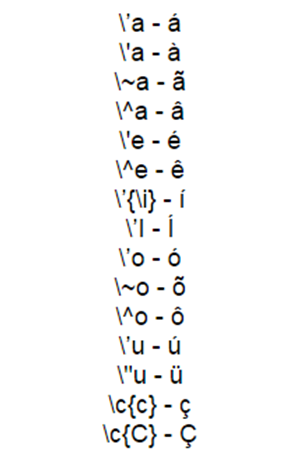
\includegraphics[scale=1.0]{USPSC-img/USPSC-AcentuacaoLaTeX.png} \\
	Fonte: \citeonline{comandos}
	\end{center}	
\end{figure}

\end{anexosenv}


%---------------------------------------------------------------------
% INDICE REMISSIVO
%--------------------------------------------------------------------
%% USPSC-IndicexRemissivosTutorial.tex
% ---
% Inicia os Índices Remissivos
% ---
%---------------------------------------------------------------------
% INDICE REMISSIVO
%--------------------------------------------------------------------
\phantompart
\printindex
%---------------------------------------------------------------------


%---------------------------------------------------------------------

\end{document}
